\PassOptionsToPackage{unicode=true}{hyperref} % options for packages loaded elsewhere
\PassOptionsToPackage{hyphens}{url}
\PassOptionsToPackage{dvipsnames,svgnames*,x11names*}{xcolor}
%
\documentclass[]{krantz}
\usepackage{lmodern}
\usepackage{amssymb,amsmath}
\usepackage{ifxetex,ifluatex}
\usepackage{fixltx2e} % provides \textsubscript
\ifnum 0\ifxetex 1\fi\ifluatex 1\fi=0 % if pdftex
  \usepackage[T1]{fontenc}
  \usepackage[utf8]{inputenc}
  \usepackage{textcomp} % provides euro and other symbols
\else % if luatex or xelatex
  \usepackage{unicode-math}
  \defaultfontfeatures{Ligatures=TeX,Scale=MatchLowercase}
    \setsansfont[]{Helvetica}
    \setmonofont[Mapping=tex-ansi,Scale=0.7]{Source Code Pro}
  \setmathfont[]{STIX Two Math}
\fi
% use upquote if available, for straight quotes in verbatim environments
\IfFileExists{upquote.sty}{\usepackage{upquote}}{}
% use microtype if available
\IfFileExists{microtype.sty}{%
\usepackage[]{microtype}
\UseMicrotypeSet[protrusion]{basicmath} % disable protrusion for tt fonts
}{}
\IfFileExists{parskip.sty}{%
\usepackage{parskip}
}{% else
\setlength{\parindent}{0pt}
\setlength{\parskip}{6pt plus 2pt minus 1pt}
}
\usepackage{xcolor}
\usepackage{hyperref}
\hypersetup{
            pdftitle={Introduction to Statistical Thinking},
            pdfauthor={Benjamin Yakir},
            colorlinks=true,
            linkcolor=Maroon,
            citecolor=Blue,
            urlcolor=Blue,
            breaklinks=true}
\urlstyle{same}  % don't use monospace font for urls
\usepackage{color}
\usepackage{fancyvrb}
\newcommand{\VerbBar}{|}
\newcommand{\VERB}{\Verb[commandchars=\\\{\}]}
\DefineVerbatimEnvironment{Highlighting}{Verbatim}{commandchars=\\\{\}}
% Add ',fontsize=\small' for more characters per line
\usepackage{framed}
\definecolor{shadecolor}{RGB}{248,248,248}
\newenvironment{Shaded}{\begin{snugshade}}{\end{snugshade}}
\newcommand{\AlertTok}[1]{\textcolor[rgb]{0.94,0.16,0.16}{#1}}
\newcommand{\AnnotationTok}[1]{\textcolor[rgb]{0.56,0.35,0.01}{\textbf{\textit{#1}}}}
\newcommand{\AttributeTok}[1]{\textcolor[rgb]{0.77,0.63,0.00}{#1}}
\newcommand{\BaseNTok}[1]{\textcolor[rgb]{0.00,0.00,0.81}{#1}}
\newcommand{\BuiltInTok}[1]{#1}
\newcommand{\CharTok}[1]{\textcolor[rgb]{0.31,0.60,0.02}{#1}}
\newcommand{\CommentTok}[1]{\textcolor[rgb]{0.56,0.35,0.01}{\textit{#1}}}
\newcommand{\CommentVarTok}[1]{\textcolor[rgb]{0.56,0.35,0.01}{\textbf{\textit{#1}}}}
\newcommand{\ConstantTok}[1]{\textcolor[rgb]{0.00,0.00,0.00}{#1}}
\newcommand{\ControlFlowTok}[1]{\textcolor[rgb]{0.13,0.29,0.53}{\textbf{#1}}}
\newcommand{\DataTypeTok}[1]{\textcolor[rgb]{0.13,0.29,0.53}{#1}}
\newcommand{\DecValTok}[1]{\textcolor[rgb]{0.00,0.00,0.81}{#1}}
\newcommand{\DocumentationTok}[1]{\textcolor[rgb]{0.56,0.35,0.01}{\textbf{\textit{#1}}}}
\newcommand{\ErrorTok}[1]{\textcolor[rgb]{0.64,0.00,0.00}{\textbf{#1}}}
\newcommand{\ExtensionTok}[1]{#1}
\newcommand{\FloatTok}[1]{\textcolor[rgb]{0.00,0.00,0.81}{#1}}
\newcommand{\FunctionTok}[1]{\textcolor[rgb]{0.00,0.00,0.00}{#1}}
\newcommand{\ImportTok}[1]{#1}
\newcommand{\InformationTok}[1]{\textcolor[rgb]{0.56,0.35,0.01}{\textbf{\textit{#1}}}}
\newcommand{\KeywordTok}[1]{\textcolor[rgb]{0.13,0.29,0.53}{\textbf{#1}}}
\newcommand{\NormalTok}[1]{#1}
\newcommand{\OperatorTok}[1]{\textcolor[rgb]{0.81,0.36,0.00}{\textbf{#1}}}
\newcommand{\OtherTok}[1]{\textcolor[rgb]{0.56,0.35,0.01}{#1}}
\newcommand{\PreprocessorTok}[1]{\textcolor[rgb]{0.56,0.35,0.01}{\textit{#1}}}
\newcommand{\RegionMarkerTok}[1]{#1}
\newcommand{\SpecialCharTok}[1]{\textcolor[rgb]{0.00,0.00,0.00}{#1}}
\newcommand{\SpecialStringTok}[1]{\textcolor[rgb]{0.31,0.60,0.02}{#1}}
\newcommand{\StringTok}[1]{\textcolor[rgb]{0.31,0.60,0.02}{#1}}
\newcommand{\VariableTok}[1]{\textcolor[rgb]{0.00,0.00,0.00}{#1}}
\newcommand{\VerbatimStringTok}[1]{\textcolor[rgb]{0.31,0.60,0.02}{#1}}
\newcommand{\WarningTok}[1]{\textcolor[rgb]{0.56,0.35,0.01}{\textbf{\textit{#1}}}}
\usepackage{longtable,booktabs}
% Fix footnotes in tables (requires footnote package)
\IfFileExists{footnote.sty}{\usepackage{footnote}\makesavenoteenv{longtable}}{}
\usepackage{graphicx,grffile}
\makeatletter
\def\maxwidth{\ifdim\Gin@nat@width>\linewidth\linewidth\else\Gin@nat@width\fi}
\def\maxheight{\ifdim\Gin@nat@height>\textheight\textheight\else\Gin@nat@height\fi}
\makeatother
% Scale images if necessary, so that they will not overflow the page
% margins by default, and it is still possible to overwrite the defaults
% using explicit options in \includegraphics[width, height, ...]{}
\setkeys{Gin}{width=\maxwidth,height=\maxheight,keepaspectratio}
\setlength{\emergencystretch}{3em}  % prevent overfull lines
\providecommand{\tightlist}{%
  \setlength{\itemsep}{0pt}\setlength{\parskip}{0pt}}
\setcounter{secnumdepth}{5}
% Redefines (sub)paragraphs to behave more like sections
\ifx\paragraph\undefined\else
\let\oldparagraph\paragraph
\renewcommand{\paragraph}[1]{\oldparagraph{#1}\mbox{}}
\fi
\ifx\subparagraph\undefined\else
\let\oldsubparagraph\subparagraph
\renewcommand{\subparagraph}[1]{\oldsubparagraph{#1}\mbox{}}
\fi

% set default figure placement to htbp
\makeatletter
\def\fps@figure{htbp}
\makeatother

\usepackage{booktabs}
\usepackage{longtable}
\usepackage[bf,singlelinecheck=off]{caption}

%\setmainfont[UprightFeatures={SmallCapsFont=AlegreyaSC-Regular}]{Alegreya}

%\newcommand{\Expec}{{\rm I\kern-.3em E}}
%\newcommand{\Prob}{{\rm I\kern-.3em P}}
%\newcommand{\Var}{{\rm I\kern-.3em V}}
%\newcommand{\Cov}{{\rm I\kern-.3em Cov}}

\newcommand{\Expec}{\mathbf{E}}
\newcommand{\Prob}{\mathbf{P}}
\newcommand{\Var}{\mathbf{V}}
\newcommand{\Cov}{\mathbf{Cov}}


\usepackage{framed,color}
\definecolor{shadecolor}{RGB}{248,248,248}

\renewcommand{\textfraction}{0.05}
\renewcommand{\topfraction}{0.8}
\renewcommand{\bottomfraction}{0.8}
\renewcommand{\floatpagefraction}{0.75}

\renewenvironment{quote}{\begin{VF}}{\end{VF}}
\let\oldhref\href
\renewcommand{\href}[2]{#2\footnote{\url{#1}}}

\ifxetex
  \usepackage{letltxmacro}
  \setlength{\XeTeXLinkMargin}{1pt}
  \LetLtxMacro\SavedIncludeGraphics\includegraphics
  \def\includegraphics#1#{% #1 catches optional stuff (star/opt. arg.)
    \IncludeGraphicsAux{#1}%
  }%
  \newcommand*{\IncludeGraphicsAux}[2]{%
    \XeTeXLinkBox{%
      \SavedIncludeGraphics#1{#2}%
    }%
  }%
\fi

\makeatletter
\newenvironment{kframe}{%
\medskip{}
\setlength{\fboxsep}{.8em}
 \def\at@end@of@kframe{}%
 \ifinner\ifhmode%
  \def\at@end@of@kframe{\end{minipage}}%
  \begin{minipage}{\columnwidth}%
 \fi\fi%
 \def\FrameCommand##1{\hskip\@totalleftmargin \hskip-\fboxsep
 \colorbox{shadecolor}{##1}\hskip-\fboxsep
     % There is no \\@totalrightmargin, so:
     \hskip-\linewidth \hskip-\@totalleftmargin \hskip\columnwidth}%
 \MakeFramed {\advance\hsize-\width
   \@totalleftmargin\z@ \linewidth\hsize
   \@setminipage}}%
 {\par\unskip\endMakeFramed%
 \at@end@of@kframe}
\makeatother

\renewenvironment{Shaded}{\begin{kframe}}{\end{kframe}}

\usepackage{makeidx}
\makeindex

\urlstyle{tt}

\usepackage{amsthm}
\makeatletter
\def\thm@space@setup{%
  \thm@preskip=8pt plus 2pt minus 4pt
  \thm@postskip=\thm@preskip
}
\makeatother

\frontmatter
\usepackage[]{natbib}
\bibliographystyle{apalike}

\title{Introduction to Statistical Thinking}
\author{Benjamin Yakir}
\date{2019-01-17}

\usepackage{amsthm}
\newtheorem{theorem}{Theorem}[chapter]
\newtheorem{lemma}{Lemma}[chapter]
\newtheorem{corollary}{Corollary}[chapter]
\newtheorem{proposition}{Proposition}[chapter]
\newtheorem{conjecture}{Conjecture}[chapter]
\theoremstyle{definition}
\newtheorem{definition}{Definition}[chapter]
\theoremstyle{definition}
\newtheorem{example}{Example}[chapter]
\theoremstyle{definition}
\newtheorem{exercise}{Exercise}[chapter]
\theoremstyle{remark}
\newtheorem*{remark}{Remark}
\newtheorem*{solution}{Solution}
\let\BeginKnitrBlock\begin \let\EndKnitrBlock\end
\begin{document}
\maketitle

% you may need to leave a few empty pages before the dedication page

%\cleardoublepage\newpage\thispagestyle{empty}\null
%\cleardoublepage\newpage\thispagestyle{empty}\null
%\cleardoublepage\newpage
\thispagestyle{empty}

\begin{center}
In memory of my father, Moshe Yakir, and the family he lost.
\end{center}

\setlength{\abovedisplayskip}{-5pt}
\setlength{\abovedisplayshortskip}{-5pt}

{
\hypersetup{linkcolor=}
\setcounter{tocdepth}{2}
\tableofcontents
}
\hypertarget{preface}{%
\chapter*{Preface}\label{preface}}


The target audience for this book is college students who are required
to learn statistics, students with little background in mathematics and
often no motivation to learn more. It is assumed that the students do
have basic skills in using computers and have access to one. Moreover,
it is assumed that the students are willing to actively follow the
discussion in the text, to practice, and more importantly, to think.

Teaching statistics is a challenge. Teaching it to students who are
required to learn the subject as part of their curriculum, is an art
mastered by few. In the past I have tried to master this art and failed.
In desperation, I wrote this book.

This book uses the basic structure of generic introduction to statistics
course. However, in some ways I have chosen to diverge from the
traditional approach. One divergence is the introduction of \texttt{R} as part
of the learning process. Many have used statistical packages or
spreadsheets as tools for teaching statistics. Others have used \texttt{R} in
advanced courses. I am not aware of attempts to use \texttt{R} in introductory
level courses. Indeed, mastering \texttt{R} requires much investment of time
and energy that may be distracting and counterproductive for learning
more fundamental issues. Yet, I believe that if one restricts the
application of \texttt{R} to a limited number of commands, the benefits that
\texttt{R} provides outweigh the difficulties that \texttt{R} engenders.

Another departure from the standard approach is the treatment of
probability as part of the course. In this book I do not attempt to
teach probability as a subject matter, but only specific elements of it
which I feel are essential for understanding statistics. Hence,
Kolmogorov's Axioms are out as well as attempts to prove basic theorems
and a Balls and Urns type of discussion. On the other hand, emphasis is
given to the notion of a \emph{random variable} and, in that context, the
\emph{sample space}.

The first part of the book deals with descriptive statistics and
provides probability concepts that are required for the interpretation
of statistical inference. Statistical inference is the subject of the
second part of the book.

The first chapter is a short introduction to statistics and probability.
Students are required to have access to \texttt{R} right from the start.
Instructions regarding the installation of \texttt{R} on a PC are provided.

The second chapter deals with data structures and variation. Chapter~3
provides numerical and graphical tools for presenting and summarizing
the distribution of data.

The fundamentals of probability are treated in Chapters~4 to~7. The
concept of a random variable is presented in Chapter~4 and examples of
special types of random variables are discussed in Chapter~5. Chapter~6
deals with the Normal random variable. Chapter~7 introduces sampling
distribution and presents the Central Limit Theorem and the Law of Large
Numbers. Chapter~8 summarizes the material of the first seven chapters
and discusses it in the statistical context.

Chapter~9 starts the second part of the book and the discussion of
statistical inference. It provides an overview of the topics that are
presented in the subsequent chapter. The material of the first half is
revisited.

Chapters~10 to~12 introduce the basic tools of statistical inference,
namely point estimation, estimation with a confidence interval, and the
testing of statistical hypothesis. All these concepts are demonstrated
in the context of a single measurements.

Chapters~13 to~15 discuss inference that involve the comparison of two
measurements. The context where these comparisons are carried out is
that of regression that relates the distribution of a response to an
explanatory variable. In Chapter~13 the response is numeric and the
explanatory variable is a factor with two levels. In Chapter~14 both the
response and the explanatory variable are numeric and in Chapter~15 the
response in a factor with two levels.

Chapter~16 ends the book with the analysis of two case studies. These
analyses require the application of the tools that are presented
throughout the book.

This book was originally written for a pair of courses in the
\href{http://www.uopeople.org/}{University of the People}. As such, each part
was restricted to 8 chapters. Due to lack of space, some important
material, especially the concepts of correlation and statistical
independence were omitted. In future versions of the book I hope to fill
this gap.

Large portions of this book, mainly in the first chapters and some of
the quizzes, are based on material from the online book ``Collaborative
Statistics'' by Barbara Illowsky and Susan Dean (Connexions, March 2,
2010. \url{http://cnx.org/content/col10522/1.37/}). Most of the material was
edited by this author, who is the only person responsible for any errors
that where introduced in the process of editing.

Case studies that are presented in the second part of the book are taken
from \href{http://onlinestatbook.com/rvls.html}{Rice Virtual Lab in
Statistics} can be found in their
\href{http://onlinestatbook.com/case_studies_rvls/}{Case Studies} section.
The responsibility for mistakes in the analysis of the data, if such
mistakes are found, are my own.

I would like to thank my mother Ruth who, apart from giving birth,
feeding and educating me, has also helped to improve the pedagogical
structure of this text. I would like to thank also Gary Engstrom for
correcting many of the mistakes in English that I made.

This book is an open source and may be used by anyone who wishes to do
so. (Under the conditions of the \href{http://creativecommons.org/licenses/by/3.0/}{Creative Commons Attribution License
(CC-BY 3.0)}.))

Jerusalem, June 2011.

\mainmatter

\hypertarget{ChapIntroR}{%
\chapter{Introduction}\label{ChapIntroR}}

\hypertarget{student-learning-objectives}{%
\section{Student Learning Objectives}\label{student-learning-objectives}}

This chapter introduces the basic concepts of statistics. Special
attention is given to concepts that are used in the first part of this
book, the part that deals with graphical and numeric statistical ways to
describe data (descriptive statistics) as well as mathematical theory of
probability that enables statisticians to draw conclusions from data.

The course applies the widely used freeware programming environment for
statistical analysis, known as \texttt{R}. In this chapter we will discuss the
installation of the program and present very basic features of that
system.

By the end of this chapter, the student should be able to:

\begin{itemize}
\tightlist
\item
  Recognize key terms in statistics and probability.
\item
  Install the \texttt{R} program on an accessible computer.
\item
  Learn and apply a few basic operations of the computational system \texttt{R}.
\end{itemize}

\hypertarget{why-learn-statistics}{%
\section{Why Learn Statistics?}\label{why-learn-statistics}}

You are probably asking yourself the question, ``When and where will I
use statistics?''. If you read any newspaper or watch television, or use
the Internet, you will see statistical information. There are statistics
about crime, sports, education, politics, and real estate. Typically,
when you read a newspaper article or watch a news program on television,
you are given sample information. With this information, you may make a
decision about the correctness of a statement, claim, or ``fact''.
Statistical methods can help you make the ``best educated guess''.

Since you will undoubtedly be given statistical information at some
point in your life, you need to know some techniques to analyze the
information thoughtfully. Think about buying a house or managing a
budget. Think about your chosen profession. The fields of economics,
business, psychology, education, biology, law, computer science, police
science, and early childhood development require at least one course in
statistics.

Included in this chapter are the basic ideas and words of probability
and statistics. In the process of learning the first part of the book,
and more so in the second part of the book, you will understand that
statistics and probability work together.

\hypertarget{statistics}{%
\section{Statistics}\label{statistics}}

The science of statistics deals with the collection, analysis,
interpretation, and presentation of data. We see and use data in our
everyday lives. To be able to use data correctly is essential to many
professions and is in your own best self-interest.

\begin{figure}

{\centering 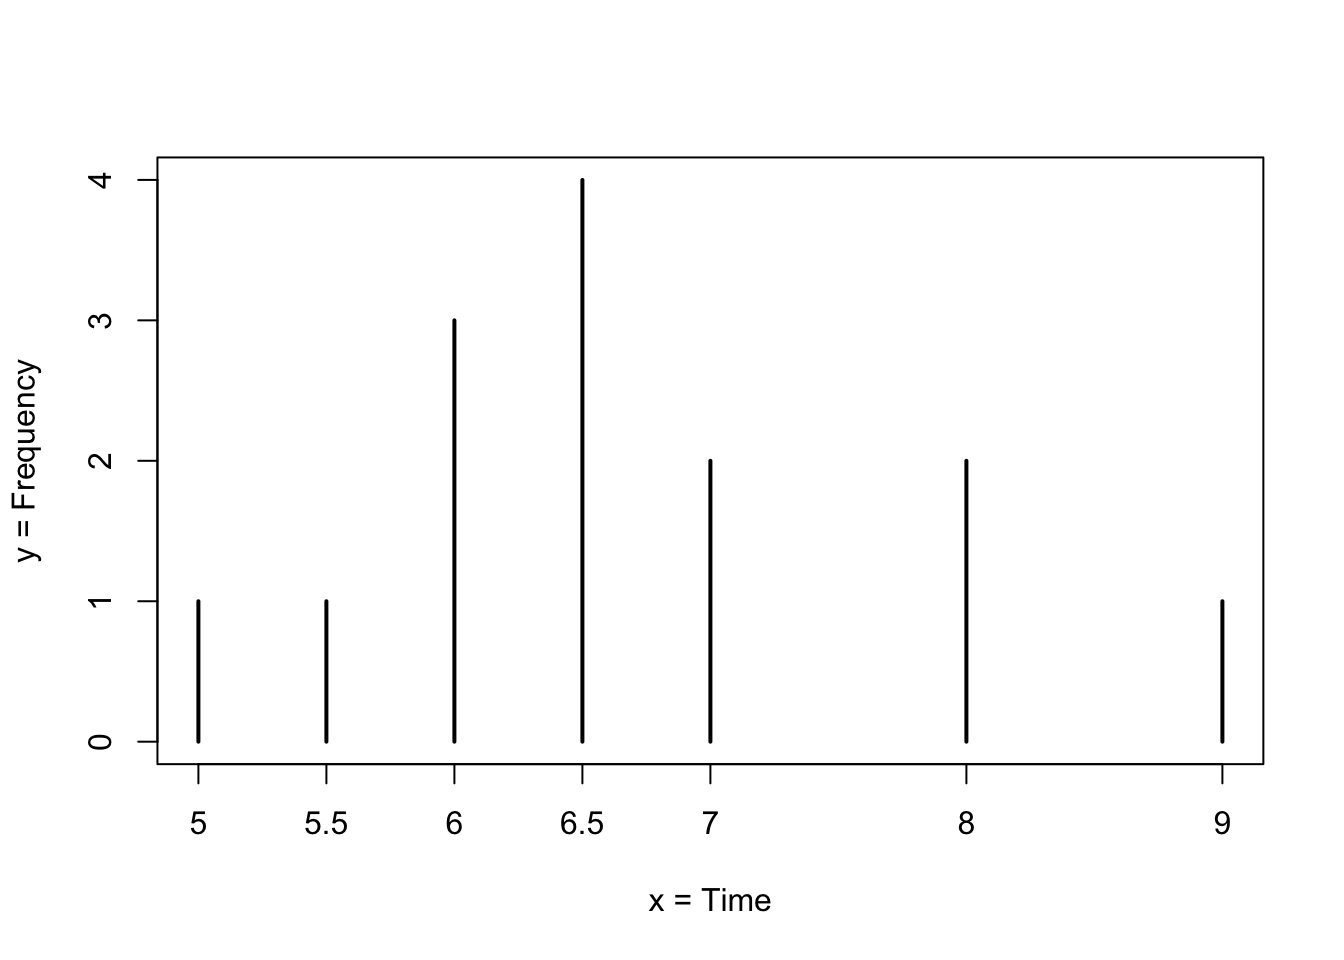
\includegraphics[width=0.6\linewidth]{statthink_files/figure-latex/intror1-1} 

}

\caption{Frequency of Average Time (in Hours) Spent Sleeping per Night}\label{fig:intror1}
\end{figure}

For example, assume the average time (in hours, to the nearest
half-hour) a group of people sleep per night has been recorded. Consider
the following data:

\[5,\; 5.5,\; 6,\; 6,\; 6,\; 6.5,\; 6.5,\; 6.5,\; 6.5,\; 7,\; 7,\; 8,\; 8,\; 9\;.\]

In Figure~\ref{fig:intror1} this data is presented in a graphical form
(called a bar plot). A bar plot consists of a number axis (the \(x\)-axis)
and bars (vertical lines) positioned above the number axis. The length
of each bar corresponds to the number of data points that obtain the
given numerical value. In the given plot the frequency of average time
(in hours) spent sleeping per night is presented with hours of sleep on
the horizontal \(x\)-axis and frequency on vertical \(y\)-axis.

Think of the following questions:

\begin{itemize}
\item
  Would the bar plot constructed from data collected from a different
  group of people look the same as or different from the example? Why?
\item
  If one would have carried the same example in a different group with
  the same size and age as the one used for the example, do you think
  the results would be the same? Why or why not?
\item
  Where does the data appear to cluster? How could you interpret the
  clustering?
\end{itemize}

The questions above ask you to analyze and interpret your data. With
this example, you have begun your study of statistics.

In this course, you will learn how to organize and summarize data.
Organizing and summarizing data is called descriptive statistics. Two
ways to summarize data are by graphing and by numbers (for example,
finding an average). In the second part of the book you will also learn
how to use formal methods for drawing conclusions from ``good'' data. The
formal methods are called inferential statistics. Statistical inference
uses probabilistic concepts to determine if conclusions drawn are
reliable or not.

Effective interpretation of data is based on good procedures for
producing data and thoughtful examination of the data. In the process of
learning how to interpret data you will probably encounter what may seem
to be too many mathematical formulae that describe these procedures.
However, you should always remember that the goal of statistics is not
to perform numerous calculations using the formulae, but to gain an
understanding of your data. The calculations can be done using a
calculator or a computer. The understanding must come from you. If you
can thoroughly grasp the basics of statistics, you can be more confident
in the decisions you make in life.

\hypertarget{probability}{%
\section{Probability}\label{probability}}

Probability is the mathematical theory used to study uncertainty. It
provides tools for the formalization and quantification of the notion of
uncertainty. In particular, it deals with the chance of an event
occurring. For example, if the different potential outcomes of an
experiment are equally likely to occur then the probability of each
outcome is taken to be the reciprocal of the number of potential
outcomes. As an illustration, consider tossing a fair coin. There are
two possible outcomes -- a head or a tail -- and the probability of each
outcome is \(1/2\).

If you toss a fair coin 4 times, the outcomes may not necessarily be 2
heads and 2 tails. However, if you toss the same coin 4,000 times, the
outcomes will be close to 2,000 heads and 2,000 tails. It is very
unlikely to obtain more than 2,060 tails and it is similarly unlikely to
obtain less than 1,940 tails. This is consistent with the expected
theoretical probability of heads in any one toss. Even though the
outcomes of a few repetitions are uncertain, there is a regular pattern
of outcomes when the number of repetitions is large. Statistics exploits
this pattern regularity in order to make extrapolations from the
observed sample to the entire population.

The theory of probability began with the study of games of chance such
as poker. Today, probability is used to predict the likelihood of an
earthquake, of rain, or whether you will get an ``A'' in this course.
Doctors use probability to determine the chance of a vaccination causing
the disease the vaccination is supposed to prevent. A stockbroker uses
probability to determine the rate of return on a client's investments.
You might use probability to decide to buy a lottery ticket or not.

Although probability is instrumental for the development of the theory
of statistics, in this introductory course we will not develop the
mathematical theory of probability. Instead, we will concentrate on the
philosophical aspects of the theory and use computerized simulations in
order to demonstrate probabilistic computations that are applied in
statistical inference.

\hypertarget{key-terms}{%
\section{Key Terms}\label{key-terms}}

In statistics, we generally want to study a population. You can think of
a population as an entire collection of persons, things, or objects
under study. To study the larger population, we select a sample. The
idea of sampling is to select a portion (or subset) of the larger
population and study that portion (the sample) to gain information about
the population. Data are the result of sampling from a population.

Because it takes a lot of time and money to examine an entire
population, sampling is a very practical technique. If you wished to
compute the overall grade point average at your school, it would make
sense to select a sample of students who attend the school. The data
collected from the sample would be the students' grade point averages.
In presidential elections, opinion poll samples of 1,000 to 2,000 people
are taken. The opinion poll is supposed to represent the views of the
people in the entire country. Manufacturers of canned carbonated drinks
take samples to determine if the manufactured 16 ounce containers does
indeed contain 16 ounces of the drink.

From the sample data, we can calculate a \emph{statistic}. A statistic is a
number that is a property of the sample. For example, if we consider one
math class to be a sample of the population of all math classes, then
the average number of points earned by students in that one math class
at the end of the term is an example of a statistic. The statistic can
be used as an estimate of a population \emph{parameter}. A parameter is a
number that is a property of the population. Since we considered all
math classes to be the population, then the average number of points
earned per student over all the math classes is an example of a
parameter.

One of the main concerns in the field of statistics is how accurately a
statistic estimates a parameter. The accuracy really depends on how well
the sample represents the population. The sample must contain the
characteristics of the population in order to be a representative
sample.

Two words that come up often in statistics are \emph{average} and
\emph{proportion}. If you were to take three exams in your math classes and
obtained scores of 86, 75, and 92, you calculate your average score by
adding the three exam scores and dividing by three (your average score
would be 84.3 to one decimal place). If, in your math class, there are
40 students and 22 are men and 18 are women, then the proportion of men
students is \(22/40\) and the proportion of women students is \(18/40\).
Average and proportion are discussed in more detail in later chapters.

\hypertarget{the-r-programming-environment}{%
\section{\texorpdfstring{The \texttt{R} Programming Environment}{The R Programming Environment}}\label{the-r-programming-environment}}

The \texttt{R} Programming Environment is a widely used open source system for
statistical analysis and statistical programming. It includes thousands
of functions for the implementation of both standard and exotic
statistical methods and it is probably the most popular system in the
academic world for the development of new statistical tools. We will use
\texttt{R} in order to apply the statistical methods that will be discussed in
the book to some example data sets and in order to demonstrate, via
simulations, concepts associated with probability and its application in
statistics.

The demonstrations in the book involve very basic \texttt{R} programming skills
and the applications are implemented using, in most cases, simple and
natural code. A detailed explanation will accompany the code that is
used.

Learning \texttt{R}, like the learning of any other programming language, can
be achieved only through practice. Hence, we strongly recommend that you
not only read the code presented in the book but also run it yourself,
in parallel to the reading of the provided explanations. Moreover, you
are encouraged to play with the code: introduce changes in the code and
in the data and see how the output changes as a result. One should not
be afraid to experiment. At worst, the computer may crash or freeze. In
both cases, restarting the computer will solve the problem \ldots{}

You may download \texttt{R} from the \texttt{R} project home
page~\url{http://www.r-project.org} and install it on the computer that you
are using\footnote{Detailed explanation of how to install the system on an XP Windows
  Operating System may be found here:
  \url{http://pluto.huji.ac.il/~msby/StatThink/install_R_WinXP.html}.}.

\hypertarget{some-basic-r-commands}{%
\subsection{\texorpdfstring{Some Basic \texttt{R} Commands}{Some Basic R Commands}}\label{some-basic-r-commands}}

\texttt{R} is an object-oriented programming system. During the session you may
create and manipulate objects by the use of functions that are part of
the basic installation. You may also use the \texttt{R} programming language.
Most of the functions that are part of the system are themselves written
in the \texttt{R} language and one may easily write new functions or modify
existing functions to suit specific needs.

Let us start by opening the \texttt{R\ Console} window by double-clicking on the
\texttt{R} icon. Type in the \texttt{R\ Console} window, immediately after the ``\texttt{\textgreater{}}''
prompt, the expression ``\texttt{1+2}'' and then hit the Return key. (Do not
include the double quotation in the expression that you type!):

\begin{Shaded}
\begin{Highlighting}[]
\DecValTok{1} \OperatorTok{+}\StringTok{ }\DecValTok{2}
\end{Highlighting}
\end{Shaded}

\begin{verbatim}
## [1] 3
\end{verbatim}

The prompt ``\texttt{\textgreater{}}'' indicates that the system is ready to receive commands.
Writing an expression, such as ``\texttt{1+2}'', and hitting the Return key sends
the expression to be executed. The execution of the expression may
produce an object, in this case an object that is composed of a single
number, the number ``3''.

Whenever required, the \texttt{R} system takes an action. If no other
specifications are given regarding the required action then the system
will apply the pre-programmed action. This action is called the
\emph{default} action. In the case of hitting the Return key after the
expression that we wrote the default is to display the produced object
on the screen.

Next, let us demonstrate \texttt{R} in a more meaningful way by using it in
order to produce the bar-plot of Figure~\ref{fig:intror1}. First we have
to input the data. We will produce a sequence of numbers that form the
data\footnote{In \texttt{R}, a sequence of numbers is called a \emph{vector}. However, we
  will use the term \emph{sequence} to refer to vectors.}. For that we will use the function ``\texttt{c}'' that combines its
arguments and produces a sequence with the arguments as the components
of the sequence. Write the expression:

\begin{Shaded}
\begin{Highlighting}[]
\KeywordTok{c}\NormalTok{(}\DecValTok{5}\NormalTok{,}\FloatTok{5.5}\NormalTok{,}\DecValTok{6}\NormalTok{,}\DecValTok{6}\NormalTok{,}\DecValTok{6}\NormalTok{,}\FloatTok{6.5}\NormalTok{,}\FloatTok{6.5}\NormalTok{,}\FloatTok{6.5}\NormalTok{,}\FloatTok{6.5}\NormalTok{,}\DecValTok{7}\NormalTok{,}\DecValTok{7}\NormalTok{,}\DecValTok{8}\NormalTok{,}\DecValTok{8}\NormalTok{,}\DecValTok{9}\NormalTok{)}
\end{Highlighting}
\end{Shaded}

at the prompt and hit return. The result should look like this:

\begin{verbatim}
##  [1] 5.0 5.5 6.0 6.0 6.0 6.5 6.5 6.5 6.5 7.0 7.0 8.0 8.0 9.0
\end{verbatim}

The function ``\texttt{c}'' is an example of an \texttt{R} function. A function has a
name, ``\texttt{c}'' in this case, that is followed by brackets that include the
input to the function. We call the components of the input the
\emph{arguments} of the function. Arguments are separated by commas. A
function produces an output, which is typically an \texttt{R} object. In the
current example an object of the form of a sequence was created and,
according to the default application of the system, was sent to the
screen and not saved.

If we want to create an object for further manipulation then we should
save it and give it a name. For example, it we want to save the vector
of data under the name ``\texttt{X}'' we may write the following expression at
the prompt (and then hit return):

\begin{Shaded}
\begin{Highlighting}[]
\NormalTok{X <-}\StringTok{ }\KeywordTok{c}\NormalTok{(}\DecValTok{5}\NormalTok{,}\FloatTok{5.5}\NormalTok{,}\DecValTok{6}\NormalTok{,}\DecValTok{6}\NormalTok{,}\DecValTok{6}\NormalTok{,}\FloatTok{6.5}\NormalTok{,}\FloatTok{6.5}\NormalTok{,}\FloatTok{6.5}\NormalTok{,}\FloatTok{6.5}\NormalTok{,}\DecValTok{7}\NormalTok{,}\DecValTok{7}\NormalTok{,}\DecValTok{8}\NormalTok{,}\DecValTok{8}\NormalTok{,}\DecValTok{9}\NormalTok{)}
\end{Highlighting}
\end{Shaded}

The arrow that appears after the ``\texttt{X}'' is produced by typing the less
than key ``\texttt{\textless{}}'' followed by the minus key ``\texttt{-}''. This arrow is the
assignment operator.

Observe that you may save typing by calling and editing lines of code
that were processes in an earlier part of the session. One may browse
through the lines using the up and down arrows on the right-hand side of
the keyboard and use the right and left arrows to move along the line
presented at the prompt. For example, the last expression may be
produced by finding first the line that used the function ``\texttt{c}'' with the
up and down arrow and then moving to the beginning of the line with the
left arrow. At the beginning of the line all one has to do is type
``\texttt{X\ \textless{}-}'' and hit the Return key.

Notice that no output was sent to the screen. Instead, the output from
the ``\texttt{c}'' function was assigned to an object that has the name ``\texttt{X}''. A
new object by the given name was formed and it is now available for
further analysis. In order to verify this you may write ``\texttt{X}'' at the
prompt and hit return:

\begin{Shaded}
\begin{Highlighting}[]
\NormalTok{X}
\end{Highlighting}
\end{Shaded}

\begin{verbatim}
##  [1] 5.0 5.5 6.0 6.0 6.0 6.5 6.5 6.5 6.5 7.0 7.0 8.0 8.0 9.0
\end{verbatim}

The content of the object ``\texttt{X}'' is sent to the screen, which is the
default output. Notice that we have not changed the given object, which
is still in the memory.

\begin{figure}

{\centering 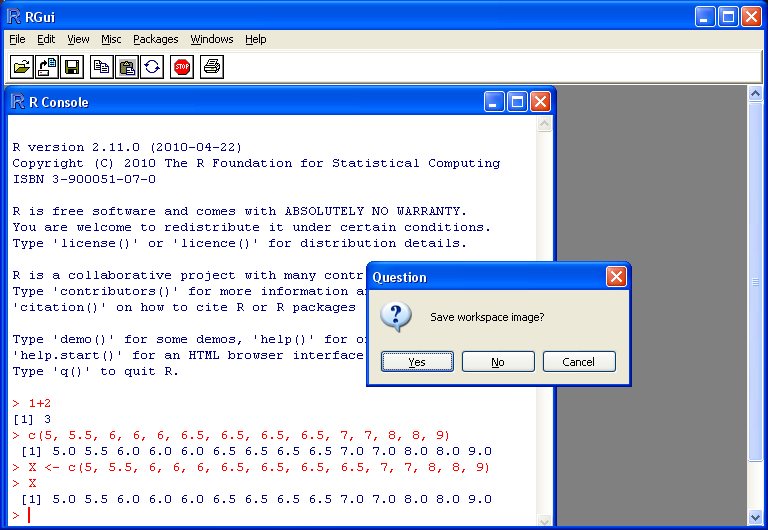
\includegraphics[width=0.6\linewidth]{_figures/8-R-Close} 

}

\caption{Save Workspace Dialog}\label{fig:fig2}
\end{figure}

The object ``\texttt{X}'' is in the memory, but it is not saved on the hard disk.
With the end of the session the objects created in the session are
erased unless specifically saved. The saving of all the objects that
were created during the session can be done when the session is
finished. Hence, when you close the \texttt{R\ Console} window a dialog box will
open (See the screenshot in Figure~\ref{fig:fig2}. Via this dialog
box you can choose to save the objects that were created in the session
by selecting ``\texttt{Yes}'', not to save by selecting the option ``\texttt{No}'', or you
may decide to abort the process of shutting down the session by
selecting ``\texttt{Cancel}''. If you save the objects then they will be uploaded
to the memory the next time that the \texttt{R\ Console} is opened.

We used a capital letter to name the object. We could have used a small
letter just as well or practically any combination of letters. However,
you should note that \texttt{R} distinguishes between capital and small letter.
Hence, typing ``\texttt{x}'' in the console window and hitting return will
produce an error message:

\begin{Shaded}
\begin{Highlighting}[]
\NormalTok{x}
\end{Highlighting}
\end{Shaded}

\begin{verbatim}
## Error in eval(expr, envir, enclos): object 'x' not found
\end{verbatim}

An object named ``\texttt{x}'' does not exist in the \texttt{R} system and we have not
created such object. The object ``\texttt{X}'', on the other hand, does exist.

Names of functions that are part of the system are fixed but you are
free to choose a name to objects that you create. For example, if one
wants to create an object by the name ``\texttt{my.vector}'' that contains the
numbers 3, 7, 3, 3, and -5 then one may write the expression
``\texttt{my.vector\ \textless{}-\ c(3,7,3,3,-5)}'' at the prompt and hit the Return key.

If we want to produce a table that contains a count of the frequency of
the different values in our data we can apply the function ``\texttt{table}'' to
the object ``\texttt{X}'' (which is the object that contains our data):

\begin{Shaded}
\begin{Highlighting}[]
\KeywordTok{table}\NormalTok{(X)}
\end{Highlighting}
\end{Shaded}

\begin{verbatim}
## X
##   5 5.5   6 6.5   7   8   9 
##   1   1   3   4   2   2   1
\end{verbatim}

Notice that the output of the function ``\texttt{table}'' is a table of the
different levels of the input vector and the frequency of each level.
This output is yet another type of an object.

The bar-plot of Figure~\ref{fig:intror1} can be produced by the
application of the function ``\texttt{plot}'' to the object that is produced as
an output of the function ``\texttt{table}'':

\begin{Shaded}
\begin{Highlighting}[]
\KeywordTok{plot}\NormalTok{(}\KeywordTok{table}\NormalTok{(X))}
\end{Highlighting}
\end{Shaded}

\begin{center}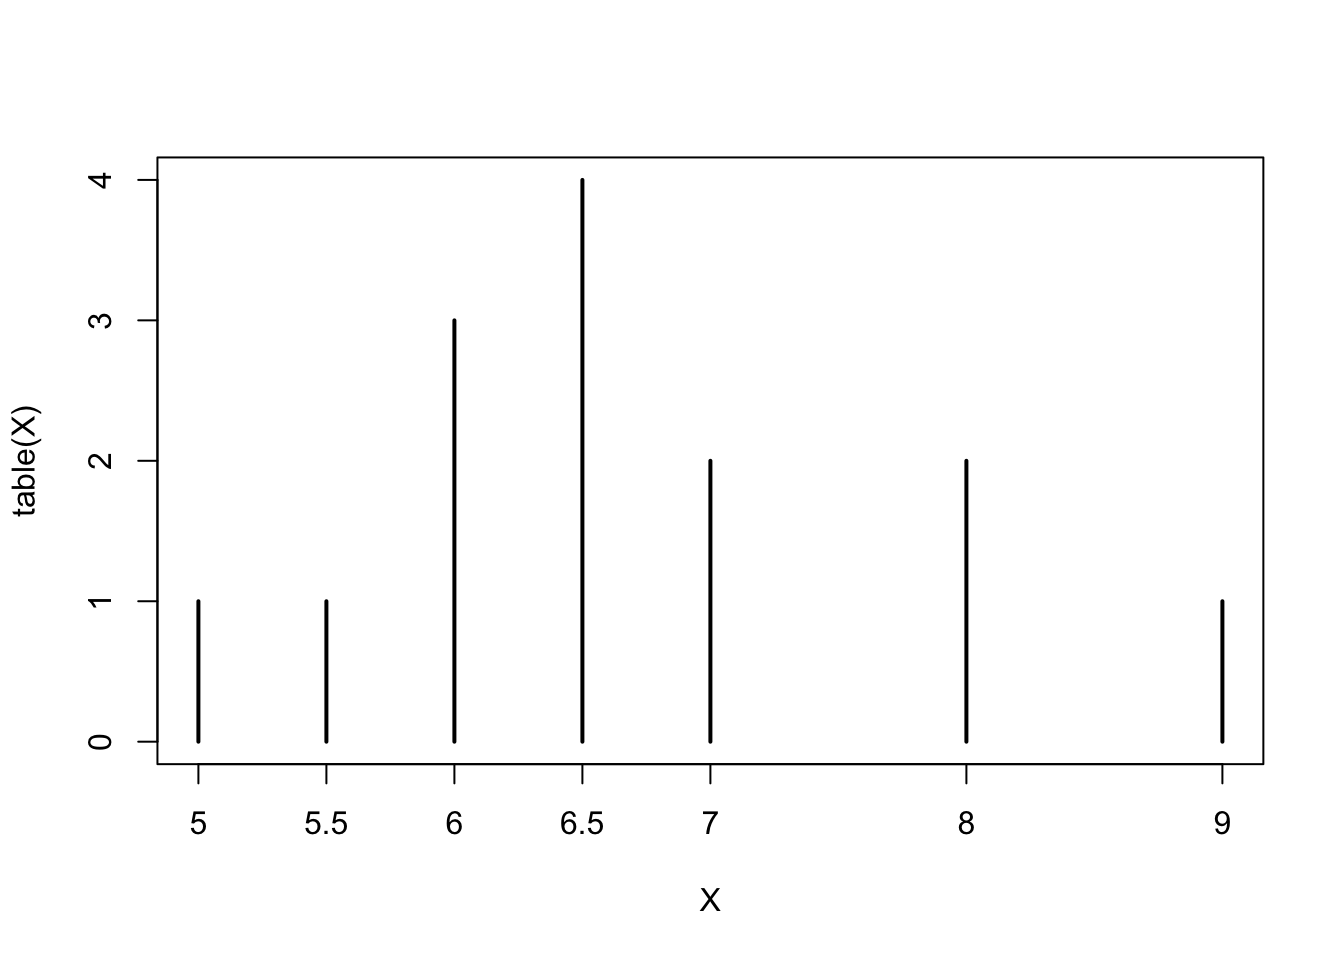
\includegraphics[width=0.6\linewidth]{statthink_files/figure-latex/unnamed-chunk-8-1} \end{center}

This plot is practically identical to the
plot in Figure~\ref{fig:intror1}. The only difference is in the names
given to the access. These names were changed in
Figure~\ref{fig:intror1} for clarity.

Clearly, if one wants to produce a bar-plot to other numerical data all
one has to do is replace in the expression \texttt{plot(table(X))} the object
\texttt{X} by an object that contains the other data. For example, to plot
the data in \texttt{my.vector} you may use \texttt{plot(table(my.vector))}.

\hypertarget{exercises}{%
\section{Exercises}\label{exercises}}

\BeginKnitrBlock{exercise}
\protect\hypertarget{exr:unnamed-chunk-9}{}{\label{exr:unnamed-chunk-9} }A potential candidate for a political position in some
state is interested to know what are her chances to win the primaries of
her party and be selected as parties candidate for the position. In
order to examine the opinions of her party voters she hires the services
of a polling agency. The polling is conducted among 500 registered
voters of the party. One of the questions that the pollsters refers to
the willingness of the voters to vote for a female candidate for the
job. Forty two percent of the people asked said that they prefer to have
a women running for the job. Thirty eight percent said that the
candidate's gender is irrelevant. The rest prefers a male candidate.
Which of the following is (i) a population (ii) a sample (iii) a
parameter and (iv) a statistic:

\begin{enumerate}
\def\labelenumi{\arabic{enumi}.}
\item
  The 500 registered voters.
\item
  The percentage, among all registered voters of the given party, of
  those that prefer a male candidate.
\item
  The number 42\% that corresponds to the percentage of those that
  prefer a female candidate.
\item
  The voters in the state that are registered to the given party.
\end{enumerate}
\EndKnitrBlock{exercise}

\BeginKnitrBlock{exercise}
\protect\hypertarget{exr:unnamed-chunk-10}{}{\label{exr:unnamed-chunk-10} }The number of customers that wait in front of a coffee
shop at the opening was reported during 25 days. The results were:

\[4,2,1,1,0,2,1,2,4,2,5,3,1,5,1,5,1,2,1,1,3,4,2,4,3\]

\begin{enumerate}
\def\labelenumi{\arabic{enumi}.}
\item
  Identify the number of days in which 5 costumers where waiting.
\item
  The number of waiting costumers that occurred the largest number of
  times.
\item
  The number of waiting costumers that occurred the least number of
  times.
\end{enumerate}
\EndKnitrBlock{exercise}

\hypertarget{summary}{%
\section{Summary}\label{summary}}

\hypertarget{glossary}{%
\subsection*{Glossary}\label{glossary}}


\begin{description}
\item[Data:]
A set of observations taken on a sample from a population.
\item[Statistic:]
A numerical characteristic of the data. A statistic estimates the
corresponding population parameter. For example, the average number
of contribution to the course's forum for this term is an estimate
for the average number of contributions in all future terms
(parameter).
\item[Statistics]
The science that deals with processing, presentation and inference
from data.
\item[Probability:]
A mathematical field that models and investigates the notion of
randomness.
\end{description}

\hypertarget{discuss-in-the-forum}{%
\subsection*{Discuss in the forum}\label{discuss-in-the-forum}}


A sample is a subgroup of the population that is supposed to represent
the entire population. In your opinion, is it appropriate to attempt to
represent the entire population only by a sample?

When you formulate your answer to this question it may be useful to come
up with an example of a question from you own field of interest one may
want to investigate. In the context of this example you may identify a
target population which you think is suited for the investigation of the
given question. The appropriateness of using a sample can be discussed
in the context of the example question and the population you have
identified.

\hypertarget{ChapData}{%
\chapter{Sampling and Data Structures}\label{ChapData}}

\hypertarget{student-learning-objectives-1}{%
\section{Student Learning Objectives}\label{student-learning-objectives-1}}

In this chapter we deal with issues associated with the data that is
obtained from a sample. The variability associated with this data is
emphasized and critical thinking about validity of the data encouraged.
A method for the introduction of data from an external source into \texttt{R}
is proposed and the data types used by \texttt{R} for storage are described. By
the end of this chapter, the student should be able to:

\begin{itemize}
\tightlist
\item
  Recognize potential difficulties with sampled data.
\item
  Read an external data file into \texttt{R}.
\item
  Create and interpret frequency tables.
\end{itemize}

\hypertarget{the-sampled-data}{%
\section{The Sampled Data}\label{the-sampled-data}}

The aim in statistics is to learn the characteristics of a population on
the basis of a sample selected from the population. An essential part of
this analysis involves consideration of variation in the data.

\hypertarget{variation-in-data}{%
\subsection{Variation in Data}\label{variation-in-data}}

Variation is given a central role in statistics. To some extent the
assessment of variation and the quantification of its contribution to
uncertainties in making inference is the statistician's main concern.

Variation is present in any set of data. For example, 16-ounce cans of
beverage may contain more or less than 16 ounces of liquid. In one
study, eight 16 ounce cans were measured and produced the following
amount (in ounces) of beverage:

\[15.8,16.1,15.2,14.8,15.8,15.9,16.0,15.5\]
Measurements of the amount of beverage in a 16-ounce may vary because
the conditions of measurement varied or because the exact amount, 16
ounces of liquid, was not put into the cans. Manufacturers regularly run
tests to determine if the amount of beverage in a 16-ounce can falls
within the desired range.

Be aware that if an investigator collects data, the data may vary
somewhat from the data someone else is taking for the same purpose. This
is completely natural. However, if two investigators or more, are taking
data from the same source and get very different results, it is time for
them to reevaluate their data-collection methods and data recording
accuracy.

\hypertarget{variation-in-samples}{%
\subsection{Variation in Samples}\label{variation-in-samples}}

Two or more samples from the same population, all having the same
characteristics as the population, may nonetheless be different from
each other. Suppose Doreen and Jung both decide to study the average
amount of time students sleep each night and use all students at their
college as the population. Doreen may decide to sample randomly a given
number of students from the entire body of collage students. Jung, on
the other hand, may decide to sample randomly a given number of classes
and survey all students in the selected classes. Doreen's method is
called \emph{random sampling} whereas Jung's method is called \emph{cluster
sampling}. Doreen's sample will be different from Jung's sample even
though both samples have the characteristics of the population. Even if
Doreen and Jung used the same sampling method, in all likelihood their
samples would be different. Neither would be wrong, however.

If Doreen and Jung took larger samples (i.e.~the number of data values
is increased), their sample results (say, the average amount of time a
student sleeps) would be closer to the actual population average. But
still, their samples would be, most probably, different from each other.

The size of a sample (often called the number of observations) is
important. The examples you have seen in this book so far have been
small. Samples of only a few hundred observations, or even smaller, are
sufficient for many purposes. In polling, samples that are from 1200 to
1500 observations are considered large enough and good enough if the
survey is random and is well done. The theory of statistical inference,
that is the subject matter of the second part of this book, provides
justification for these claims.

\hypertarget{frequency}{%
\subsection{Frequency}\label{frequency}}

The primary way of summarizing the variability of data is via the
frequency distribution. Consider an example. Twenty students were asked
how many hours they worked per day. Their responses, in hours, are
listed below:

\[5,\; 6,\; 3,\; 3,\; 2,\; 4,\; 7,\; 5,\; 2,\; 3,\; 5,\; 6,\; 5,\; 4,\; 4,\; 3,\; 5,\; 2,\; 5,\; 3\]
Let us create an \texttt{R} object by the name ``\texttt{work.hours}'' that contains
these data:

\begin{Shaded}
\begin{Highlighting}[]
\NormalTok{work.hours <-}\StringTok{ }\KeywordTok{c}\NormalTok{(}\DecValTok{5}\NormalTok{,}\DecValTok{6}\NormalTok{,}\DecValTok{3}\NormalTok{,}\DecValTok{3}\NormalTok{,}\DecValTok{2}\NormalTok{,}\DecValTok{4}\NormalTok{,}\DecValTok{7}\NormalTok{,}\DecValTok{5}\NormalTok{,}\DecValTok{2}\NormalTok{,}\DecValTok{3}\NormalTok{,}\DecValTok{5}\NormalTok{,}\DecValTok{6}\NormalTok{,}\DecValTok{5}\NormalTok{,}\DecValTok{4}\NormalTok{,}\DecValTok{4}\NormalTok{,}\DecValTok{3}\NormalTok{,}\DecValTok{5}\NormalTok{,}\DecValTok{2}\NormalTok{,}\DecValTok{5}\NormalTok{,}\DecValTok{3}\NormalTok{)}
\end{Highlighting}
\end{Shaded}

Next, let us create a table that summarizes the different values of
working hours and the frequency in which these values appear in the
data:

\begin{Shaded}
\begin{Highlighting}[]
\KeywordTok{table}\NormalTok{(work.hours)}
\end{Highlighting}
\end{Shaded}

\begin{verbatim}
## work.hours
## 2 3 4 5 6 7 
## 3 5 3 6 2 1
\end{verbatim}

Recall that the function ``\texttt{table}'' takes as input a sequence of data and
produces as output the frequencies of the different values.

We may have a clearer understanding of the meaning of the output of the
function ``\texttt{table}'' if we presented outcome as a frequency listing the
different data values in ascending order and their frequencies. For that
end we may apply the function ``\texttt{data.frame}'' to the output of the
``\texttt{table}'' function and obtain:

\begin{Shaded}
\begin{Highlighting}[]
\KeywordTok{data.frame}\NormalTok{(}\KeywordTok{table}\NormalTok{(work.hours))}
\end{Highlighting}
\end{Shaded}

\begin{verbatim}
##   work.hours Freq
## 1          2    3
## 2          3    5
## 3          4    3
## 4          5    6
## 5          6    2
## 6          7    1
\end{verbatim}

A frequency is the number of times a given datum occurs in a data set.
According to the table above, there are three students who work 2 hours,
five students who work 3 hours, etc. The total of the frequency column,
20, represents the total number of students included in the sample.

The function ``\texttt{data.frame}'' transforms its input into a data frame,
which is the standard way of storing statistical data. We will introduce
data frames in more detail in Section~\ref{readingdata} below.

A relative frequency is the fraction of times a value occurs. To find
the relative frequencies, divide each frequency by the total number of
students in the sample -- 20 in this case. Relative frequencies can be
written as fractions, percents, or decimals.

As an illustration let us compute the relative frequencies in our data:

\begin{Shaded}
\begin{Highlighting}[]
\NormalTok{freq <-}\StringTok{ }\KeywordTok{table}\NormalTok{(work.hours)}
\NormalTok{freq}
\end{Highlighting}
\end{Shaded}

\begin{verbatim}
## work.hours
## 2 3 4 5 6 7 
## 3 5 3 6 2 1
\end{verbatim}

\begin{Shaded}
\begin{Highlighting}[]
\KeywordTok{sum}\NormalTok{(freq)}
\end{Highlighting}
\end{Shaded}

\begin{verbatim}
## [1] 20
\end{verbatim}

\begin{Shaded}
\begin{Highlighting}[]
\NormalTok{freq}\OperatorTok{/}\KeywordTok{sum}\NormalTok{(freq)}
\end{Highlighting}
\end{Shaded}

\begin{verbatim}
## work.hours
##    2    3    4    5    6    7 
## 0.15 0.25 0.15 0.30 0.10 0.05
\end{verbatim}

We stored the frequencies in an object called ``\texttt{freq}''. The content of
the object are the frequencies 3, 5, 3, 6, 2 and 1. The function ``\texttt{sum}''
sums the components of its input. The sum of the frequencies is the
sample size , the total number of students that responded to the survey,
which is 20. Hence, when we apply the function ``\texttt{sum}'' to the object
``\texttt{freq}'' we get 20 as an output.

The outcome of dividing an object by a number is a division of each
element in the object by the given number. Therefore, when we divide
``\texttt{freq}'' by ``\texttt{sum(freq)}'' (the number 20) we get a sequence of relative
frequencies. The first entry to this sequence is \(3/20 = 0.15\), the
second entry is \(5/20 = 0.25\), and the last entry is \(1/20 = 0.05\). The
sum of the relative frequencies should always be equal to 1:

\begin{Shaded}
\begin{Highlighting}[]
\KeywordTok{sum}\NormalTok{(freq}\OperatorTok{/}\KeywordTok{sum}\NormalTok{(freq))}
\end{Highlighting}
\end{Shaded}

\begin{verbatim}
## [1] 1
\end{verbatim}

The cumulative relative frequency is the accumulation of previous
relative frequencies. To find the cumulative relative frequencies, add
all the previous relative frequencies to the relative frequency of the
current value. Alternatively, we may apply the function ``\texttt{cumsum}'' to
the sequence of relative frequencies:

\begin{Shaded}
\begin{Highlighting}[]
\KeywordTok{cumsum}\NormalTok{(freq}\OperatorTok{/}\KeywordTok{sum}\NormalTok{(freq))}
\end{Highlighting}
\end{Shaded}

\begin{verbatim}
##    2    3    4    5    6    7 
## 0.15 0.40 0.55 0.85 0.95 1.00
\end{verbatim}

Observe that the cumulative relative frequency of the smallest value 2
is the frequency of that value (0.15). The cumulative relative frequency
of the second value 3 is the sum of the relative frequency of the
smaller value (0.15) and the relative frequency of the current value
(0.25), which produces a total of \(0.15 + 0.25 = 0.40\). Likewise, for
the third value 4 we get a cumulative relative frequency of
\(0.15 + 0.25 + 0.15 = 0.55\). The last entry of the cumulative relative
frequency column is one, indicating that one hundred percent of the data
has been accumulated.

The computation of the cumulative relative frequency was carried out
with the aid of the function ``\texttt{cumsum}''. This function takes as an input
argument a numerical sequence and produces as output a numerical
sequence of the same length with the cumulative sums of the components
of the input sequence.

\hypertarget{critical-evaluation}{%
\subsection{Critical Evaluation}\label{critical-evaluation}}

Inappropriate methods of sampling and data collection may produce
samples that do not represent the target population. A naïve application
of statistical analysis to such data may produce misleading conclusions.

Consequently, it is important to evaluate critically the statistical
analyses we encounter before accepting the conclusions that are obtained
as a result of these analyses. Common problems that occurs in data that
one should be aware of include:

\begin{description}
\item[Problems with Samples:]
A sample should be representative of the population. A sample that
is not representative of the population is biased. Biased samples
may produce results that are inaccurate and not valid.
\item[Data Quality:]
Avoidable errors may be introduced to the data via inaccurate
handling of forms, mistakes in the input of data, etc. Data should
be cleaned from such errors as much as possible.
\item[Self-Selected Samples:]
Responses only by people who choose to respond, such as call-in
surveys, that are often biased.
\item[Sample Size Issues:]
Samples that are too small may be unreliable. Larger samples, when
possible, are better. In some situations, small samples are
unavoidable and can still be used to draw conclusions. Examples:
Crash testing cars, medical testing for rare conditions.
\item[Undue Influence:]
Collecting data or asking questions in a way that influences the
response.
\item[Causality:]
A relationship between two variables does not mean that one causes
the other to occur. They may both be related (correlated) because of
their relationship to a third variable.
\item[Self-Funded or Self-Interest Studies:]
A study performed by a person or organization in order to support
their claim. Is the study impartial? Read the study carefully to
evaluate the work. Do not automatically assume that the study is
good but do not automatically assume the study is bad either.
Evaluate it on its merits and the work done.
\item[Misleading Use of Data:]
Improperly displayed graphs and incomplete data.
\item[Confounding:]
Confounding in this context means confusing. When the effects of
multiple factors on a response cannot be separated. Confounding
makes it difficult or impossible to draw valid conclusions about the
effect of each factor.
\end{description}

\hypertarget{readingdata}{%
\section{\texorpdfstring{Reading Data into \texttt{R}}{Reading Data into R}}\label{readingdata}}

In the examples so far the size of the data set was very small and we
were able to input the data directly into \texttt{R} with the use of the
function ``\texttt{c}''. In more practical settings the data sets to be analyzed
are much larger and it is very inefficient to enter them manually. In
this section we learn how to upload data from a file in the Comma
Separated Values (CSV) format.

The file ``\texttt{ex1.csv}'' contains data on the sex and height of 100
individuals. This file is given in the CSV format. The file can be found
on the internet at
\url{http://pluto.huji.ac.il/~msby/StatThink/Datasets/ex1.csv}. We will
discuss the process of reading data from a file into \texttt{R} and use this
file as an illustration.

\hypertarget{saving-the-file-and-setting-the-working-directory}{%
\subsection{Saving the File and Setting the Working Directory}\label{saving-the-file-and-setting-the-working-directory}}

Before the file is read into \texttt{R} you may find it convenient to obtain a
copy of the file and store it in some directory on the computer and read
the file from that directory. We recommend that you create a special
directory in which you keep all the material associated with this
course. In the explanations provided below we assume that the directory
to which the file is stored in called ``\texttt{IntroStat}''. (See
Figure~\ref{fig:Data1}

\begin{figure}

{\centering 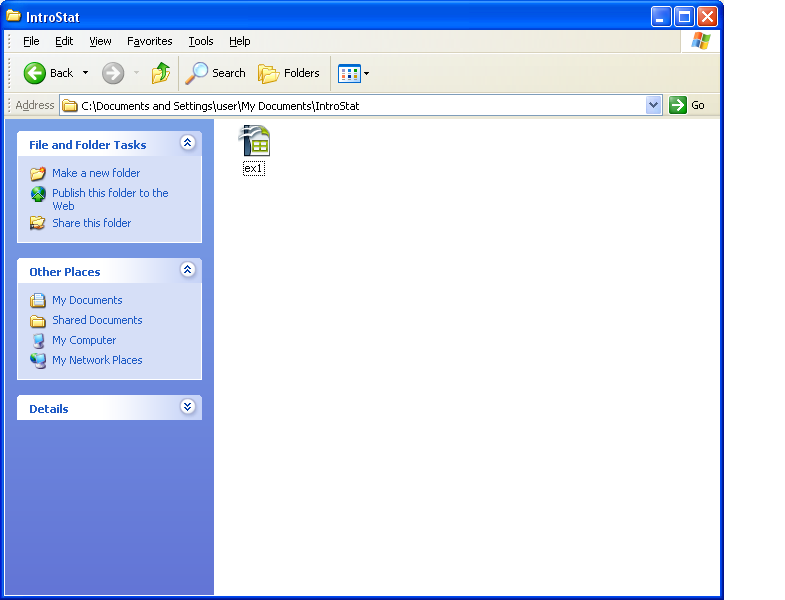
\includegraphics[width=0.6\linewidth]{_figures/Data-file} 

}

\caption{The File “`ex1.csv`"}\label{fig:Data1}
\end{figure}

Files in the CSV format are ordinary text files. They can be created
manually or as a result of converting data stored in a different format
into this particular format. A convenient way to produce, browse and
edit CSV files is by the use of a standard electronic spreadsheet
programs such as Excel or Calc. The Excel spreadsheet is part of the
Microsoft's Office suite. The Calc spreadsheet is part of the free \href{http://www.libreoffice.org/}{LibreOffice
suite}.

Opening a CSV file by a spreadsheet program displays a spreadsheet with
the content of the file. Values in the cells of the spreadsheet may be
modified directly. (However, when saving, one should pay attention to
save the file in the CVS format.) Similarly, new CSV files may be
created by the entering of the data in an empty spreadsheet. The first
row should include the name of the variable, preferably as a single
character string with no empty spaces. The following rows may contain
the data values associated with this variable. When saving, the
spreadsheet should be saved in the CSV format by the use of the ``"
dialog and choosing there the option of CSV in the ``\texttt{Save\ by\ Type}''
selection.

After saving a file with the data in a directory, \texttt{R} should be notified
where the file is located in order to be able to read it. A simple way
of doing so is by setting the directory with the file as \texttt{R}'s \emph{working
directory}. The working directory is the first place \texttt{R} is searching
for files. Files produced by \texttt{R} are saved in that directory. In
Windows, during an active \texttt{R} session, one may set the working directory
to be some target directory with the ``\texttt{File/Change\ Dir...}'' dialog. This
dialog is opened by selecting the option ``\texttt{File}'' on the left hand side
of the ruler on the top of the \texttt{R\ Console} window. Selecting the option
of ``\texttt{Change\ Dir...}'' in the ruler that opens will start the dialog. (See
Figure~\ref{fig:Data2}.) Browsing via this dialog window to the
directory of choice, selecting it, and approving the selection by
clicking the ``\texttt{OK}'' bottom in the dialog window will set the directory
of choice as the working directory of \texttt{R}.

\begin{figure}

{\centering 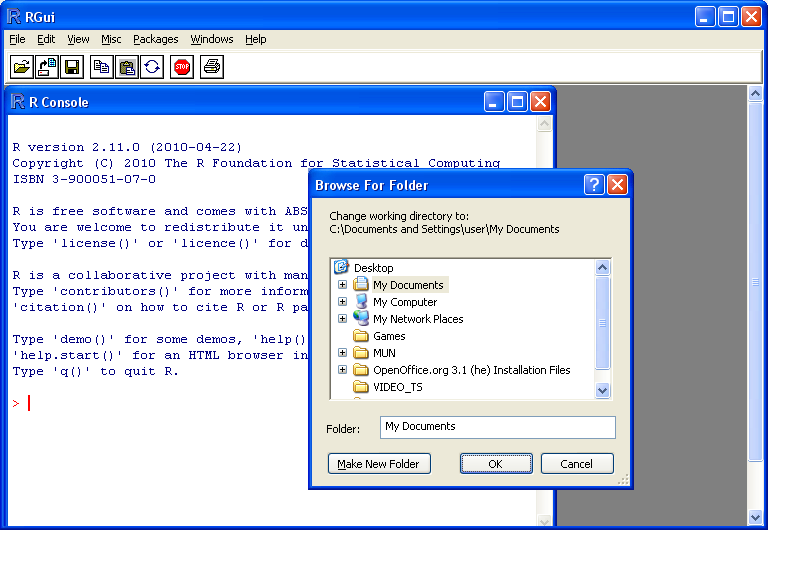
\includegraphics[width=0.6\linewidth]{_figures/Data-change-dir} 

}

\caption{Changing The Working Directory}\label{fig:Data2}
\end{figure}

Rather than changing the working directory every time that \texttt{R} is opened
one may set a selected directory to be \texttt{R}'s working directory on
opening. Again, we demonstrate how to do this on the XP Windows
operating system.

The \texttt{R} icon was added to the Desktop when the \texttt{R} system was installed.
The \texttt{R\ Console} is opened by double-clicking on this icon. One may
change the properties of the icon so that it sets a directory of choice
as \texttt{R}'s working directory.

In order to do so click on the icon with the mouse's {\textbf{right}}
bottom. A menu opens in which you should select the option
``\texttt{Properties}''. As a result, a dialog window opens. (See
Figure~\ref{fig:Data1}.) Look at the line that starts with the words
``\texttt{Start\ in}'' and continues with a name of a directory that is the
current working directory. The name of this directory is enclosed in
double quotes and is given with it's full path, i.e.~its address on the
computer. This name and path should be changed to the name and path of
the directory that you want to fix as the new working directory.

\begin{figure}

{\centering 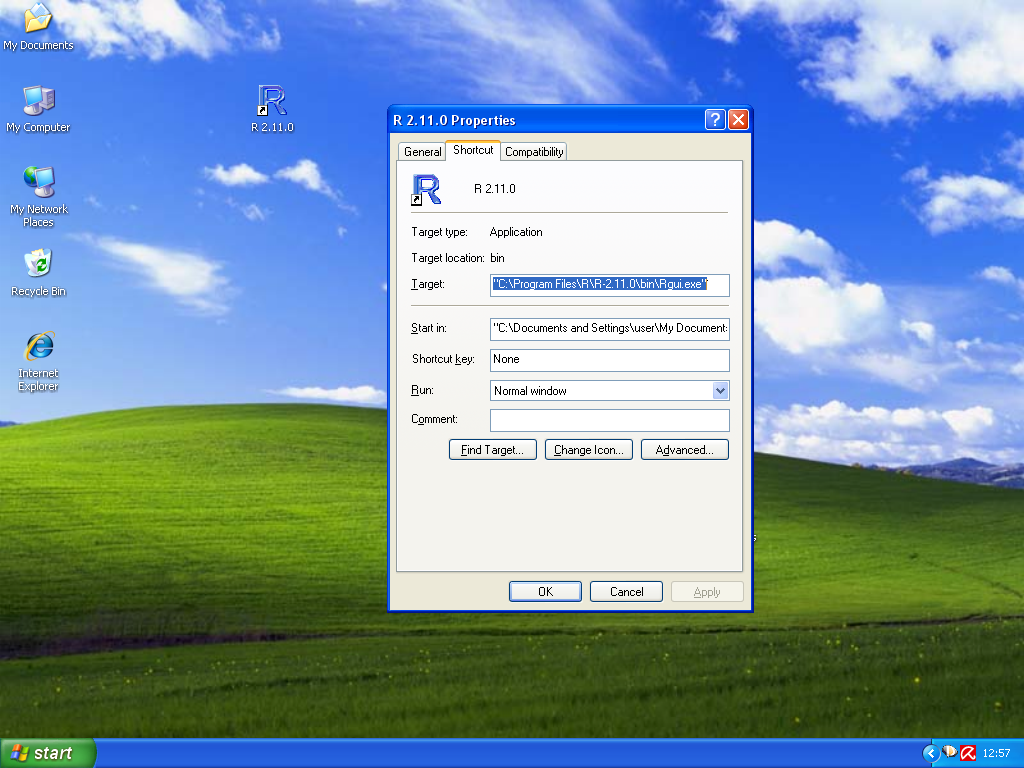
\includegraphics[width=0.6\linewidth]{_figures/Data-set-dir-before} 

}

\caption{Setting the Working Directory (Before the Change)}\label{fig:Data3}
\end{figure}

\begin{figure}

{\centering 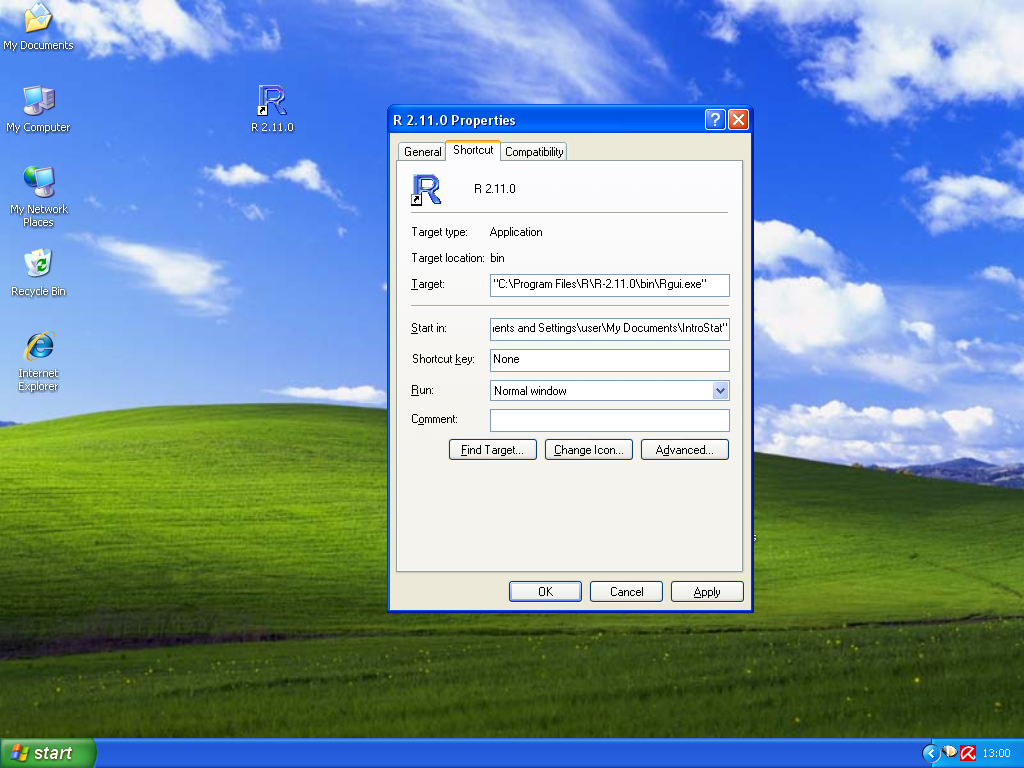
\includegraphics[width=0.6\linewidth]{_figures/Data-set-dir-after} 

}

\caption{Setting the Working Directory (After the Change)}\label{fig:Data4}
\end{figure}

Consider again Figure~\ref{fig:Data1}. Imagine that one wants to fix the
directory that contains the file ``\texttt{ex1.csv}'' as the permanent working
directory. Notice that the full address of the directory appears at the
``\texttt{Address}'' bar on the top of the window. One may copy the address and
paste it instead of the name of the current working directory that is
specified in the ``\texttt{Properties}'' dialog of the \texttt{R} icon. One should make
sure that the address to the new directory is, again, placed between
double-quotes. (See in Figure~\ref{fig:Data4} the dialog window after
the changing the address of the working directory. Compare this to
Figure~\ref{fig:Data3} of the window before the change.) After approving
the change by clicking the ``\texttt{OK}'' bottom the new working directory is
set. Henceforth, each time that the \texttt{R\ Console} is opened by
double-clicking the icon it will have the designated directory as its
working directory.

In the rest of this book we assume that a designated directory is set as
\texttt{R}'s working directory and that all external files that need to be read
into \texttt{R}, such as ``\texttt{ex1.csv}'' for example, are saved in that working
directory. Once a working directory has been set then the history of
subsequent \texttt{R} sessions is stored in that directory. Hence, if you
choose to save the image of the session when you end the session then
objects created in the session will be uploaded the next time the
\texttt{R\ Console} is opened.

\hypertarget{Data_3}{%
\subsection{\texorpdfstring{Reading a CSV File into \texttt{R}}{Reading a CSV File into R}}\label{Data_3}}

Now that a copy of the file ``\texttt{ex1.csv}'' is placed in the working
directory we would like to read its content into \texttt{R}. Reading of files
in the CSV format can be carried out with the \texttt{R} function ``\texttt{read.csv}''.
To read the file of the example we run the following line of code in the
\texttt{R\ Console} window:

\begin{Shaded}
\begin{Highlighting}[]
\NormalTok{ex}\FloatTok{.1}\NormalTok{ <-}\StringTok{ }\KeywordTok{read.csv}\NormalTok{(}\StringTok{"_data/ex1.csv"}\NormalTok{)}
\end{Highlighting}
\end{Shaded}

The function ``\texttt{read.csv}'' takes as an input argument the address of a
CSV file and produces as output a \emph{data frame} object with the content
of the file. Notice that the address is placed between double-quotes. If
the file is located in the working directory then giving the name of the
file as an address is sufficient\footnote{If the file is located in a different directory then the complete
  address, including the path to the file, should be provided. The
  file need not reside on the computer. One may provide, for example,
  a URL (an internet address) as the address. Thus, instead of saving
  the file of the example on the computer one may read its content
  into an \texttt{R} object by using the line of code
  ``\texttt{ex.1\ \textless{}-\ read.csv(http://pluto.huji.ac.il/\textasciitilde{}msby/StatThink/Datasets/ex1.csv)}''
  instead of the code that we provide and the working method that we
  recommend to follow.}.

Consider the content of that \texttt{R} object ``\texttt{ex.1}'' that was created by the
previous expression, by inspecting the first part using the function ``\texttt{head()}'':

\begin{Shaded}
\begin{Highlighting}[]
\KeywordTok{head}\NormalTok{(ex}\FloatTok{.1}\NormalTok{)}
\end{Highlighting}
\end{Shaded}

\begin{verbatim}
##        id    sex height
## 1 5696379 FEMALE    182
## 2 3019088   MALE    168
## 3 2038883   MALE    172
## 4 1920587 FEMALE    154
## 5 6006813   MALE    174
## 6 4055945 FEMALE    176
\end{verbatim}

The object ``\texttt{ex.1}'', the output of the function ``\texttt{read.csv}'' is a \emph{data
frame}. Data frames are the standard tabular format of storing
statistical data. The columns of the table are called \emph{variables} and
correspond to measurements. In this example the three variables are:

\begin{description}
\item[id:]
A 7 digits number that serves as a unique identifier of the subject.
\item[sex:]
The sex of each subject. The values are either ``\texttt{MALE}'' or
``\texttt{FEMALE}''.
\item[height:]
The height (in centimeter) of each subject. A numerical value.
\end{description}

When the values of the variable are numerical we say that it is a
\emph{quantitative variable} or a \emph{numeric variable}. On the other hand, if
the variable has qualitative or level values we say that it is a
\emph{factor}. In the given example, \texttt{sex} is a factor and \texttt{height} is a
numeric variable.

The rows of the table are called \emph{observations} and correspond to the
subjects. In this data set there are 100 subjects, with subject number
1, for example, being a female of height 182 cm and identifying number
5696379. Subject number 98, on the other hand, is a male of height 195
cm and identifying number 9383288.

\hypertarget{data-types}{%
\subsection{Data Types}\label{data-types}}

The columns of \texttt{R} data frames represent variables, i.e.~measurements
recorded for each of the subjects in the sample. \texttt{R} associates with
each variable a type that characterizes the content of the variable. The
two major types are

\begin{itemize}
\item
  Factors, or Qualitative Data. The type is ``\texttt{factor}''.
\item
  Quantitative Data. The type is ``\texttt{numeric}''.
\end{itemize}

Factors are the result of categorizing or describing attributes of a
population. Hair color, blood type, ethnic group, the car a person
drives, and the street a person lives on are examples of qualitative
data. Qualitative data are generally described by words or letters. For
instance, hair color might be black, dark brown, light brown, blonde,
gray, or red. Blood type might be AB+, O-, or B+. Qualitative data are
not as widely used as quantitative data because many numerical
techniques do not apply to the qualitative data. For example, it does
not make sense to find an average hair color or blood type.

Quantitative data are always numbers and are usually the data of choice
because there are many methods available for analyzing such data.
Quantitative data are the result of counting or measuring attributes of
a population. Amount of money, pulse rate, weight, number of people
living in your town, and the number of students who take statistics are
examples of quantitative data.

Quantitative data may be either discrete or continuous. All data that
are the result of counting are called quantitative discrete data. These
data take on only certain numerical values. If you count the number of
phone calls you receive for each day of the week, you may get results
such as 0, 1, 2, 3, etc. On the other hand, data that are the result of
measuring on a continuous scale are quantitative continuous data,
assuming that we can measure accurately. Measuring angles in radians may
result in the numbers \(\frac{\pi}{6}\), \(\frac{\pi}{3}\), \(\frac{\pi}{2}\),
\(\pi\), \(\frac{3\pi}{4}\), etc. If you and your friends carry backpacks
with books in them to school, the numbers of books in the backpacks are
discrete data and the weights of the backpacks are continuous data.

The data are the number of books students carry in their backpacks. You
sample five students. Two students carry 3 books, one student carries 4
books, one student carries 2 books, and one student carries 1 book. The
numbers of books (3, 4, 2, and 1) are the quantitative discrete data.

The data are the weights of the backpacks with the books in it. You
sample the same five students. The weights (in pounds) of their
backpacks are 6.2, 7, 6.8, 9.1, 4.3. Notice that backpacks carrying
three books can have different weights. Weights are quantitative
continuous data because weights are measured.

The data are the colors of backpacks. Again, you sample the same five
students. One student has a red backpack, two students have black
backpacks, one student has a green backpack, and one student has a gray
backpack. The colors red, black, black, green, and gray are qualitative
data.

The distinction between continuous and discrete numeric data is not
reflected usually in the statistical method that are used in order to
analyze the data. Indeed, \texttt{R} does not distinguish between these two
types of numeric data and store them both as ``\texttt{numeric}''. Consequently,
we will also not worry about the specific categorization of numeric data
and treat them as one. On the other hand, emphasis will be given to the
difference between numeric and factors data.

One may collect data as numbers and report it categorically. For
example, the quiz scores for each student are recorded throughout the
term. At the end of the term, the quiz scores are reported as A, B, C,
D, or F. On the other hand, one may code categories of qualitative data
with numerical values and report the values. The resulting data should
nonetheless be treated as a factor.

As default, \texttt{R} saves variables that contain non-numeric values as
factors. Otherwise, the variables are saved as numeric. The variable
type is important because different statistical methods are applied to
different data types. Hence, one should make sure that the variables
that are analyzed have the appropriate type. Especially that factors
using numbers to denote the levels are labeled as factors. Otherwise \texttt{R}
will treat them as quantitative data.

\hypertarget{exercises-1}{%
\section{Exercises}\label{exercises-1}}

\BeginKnitrBlock{exercise}
\protect\hypertarget{exr:unnamed-chunk-19}{}{\label{exr:unnamed-chunk-19} }Consider the following relative frequency table on
hurricanes that have made direct hits on the U.S. between 1851 and 2004
(\url{http://www.nhc.noaa.gov/gifs/table5.gif}). Hurricanes are given a
strength category rating based on the minimum wind speed generated by
the storm. Some of the entries to the table are missing.

\begin{longtable}[]{@{}crrr@{}}
\caption{Frequency of Hurricane Direct Hits}\tabularnewline
\toprule
Category & \# Direct Hits & Relative Freq. & Cum. Relative Freq.\tabularnewline
\midrule
\endfirsthead
\toprule
Category & \# Direct Hits & Relative Freq. & Cum. Relative Freq.\tabularnewline
\midrule
\endhead
1 & 109 & &\tabularnewline
2 & 72 & 0.2637 & 0.6630\tabularnewline
3 & & 0.2601 &\tabularnewline
4 & 18 & & 0.9890\tabularnewline
5 & 3 & 0.0110 & 1.0000\tabularnewline
\bottomrule
\end{longtable}

\begin{enumerate}
\def\labelenumi{\arabic{enumi}.}
\item
  What is the relative frequency of direct hits of category 1?
\item
  What is the relative frequency of direct hits of category 4 or more?
\end{enumerate}
\EndKnitrBlock{exercise}

\BeginKnitrBlock{exercise}
\protect\hypertarget{exr:unnamed-chunk-20}{}{\label{exr:unnamed-chunk-20} }The number of calves that were born to some cows during
their productive years was recorded. The data was entered into an R
object by the name ``\texttt{calves}''. Refer to the following \texttt{R} code:
\EndKnitrBlock{exercise}

\begin{verbatim}
  ```r
  freq <- table(calves)
  cumsum(freq)
  ```
  
  ```
  ##  1  2  3  4  5  6  7 
  ##  4  7 18 28 32 38 45
  ```
\end{verbatim}

\begin{enumerate}
\def\labelenumi{\arabic{enumi}.}
\item
  How many cows were involved in this study?
\item
  How many cows gave birth to a total of 4 calves?
\item
  What is the relative frequency of cows that gave birth to at least 4
  calves?
\end{enumerate}

```

\hypertarget{summary-1}{%
\section{Summary}\label{summary-1}}

\hypertarget{glossary}{%
\subsection*{Glossary}\label{glossary}}


\begin{description}
\item[Population:]
The collection, or set, of all individuals, objects, or measurements
whose properties are being studied.
\item[Sample:]
A portion of the population understudy. A sample is representative
if it characterizes the population being studied.
\item[Frequency:]
The number of times a value occurs in the data.
\item[Relative Frequency:]
The ratio between the frequency and the size of data.
\item[Cumulative Relative Frequency:]
The term applies to an ordered set of data values from smallest to
largest. The cumulative relative frequency is the sum of the
relative frequencies for all values that are less than or equal to
the given value.
\item[Data Frame:]
A tabular format for storing statistical data. Columns correspond to
variables and rows correspond to observations.
\item[Variable:]
A measurement that may be carried out over a collection of subjects.
The outcome of the measurement may be numerical, which produces a
quantitative variable; or it may be non-numeric, in which case a
factor is produced.
\item[Observation:]
The evaluation of a variable (or variables) for a given subject.
\item[CSV Files:]
A digital format for storing data frames.
\item[Factor:]
Qualitative data that is associated with categorization or the
description of an attribute.
\item[Quantitative:]
Data generated by numerical measurements.
\end{description}

\hypertarget{discuss-in-the-forum}{%
\subsection*{Discuss in the forum}\label{discuss-in-the-forum}}


Factors are qualitative data that are associated with categorization or
the description of an attribute. On the other hand, numeric data are
generated by numerical measurements. A common practice is to code the
levels of factors using numerical values. What do you think of this
practice?

In the formulation of your answer to the question you may think of an
example of factor variable from your own field of interest. You may
describe a benefit or a disadvantage that results from the use of a
numerical values to code the level of this factor.

\hypertarget{ChapDescriptiveStat}{%
\chapter{Descriptive Statistics}\label{ChapDescriptiveStat}}

\hypertarget{student-learning-objectives-2}{%
\section{Student Learning Objectives}\label{student-learning-objectives-2}}

This chapter deals with numerical and graphical ways to describe and
display data. This area of statistics is called \emph{descriptive
statistics}. You will learn to calculate and interpret these measures
and graphs. By the end of this chapter, you should be able to:

\begin{itemize}
\tightlist
\item
  Use histograms and box plots in order to display data graphically.
\item
  Calculate measures of central location: mean and median.
\item
  Calculate measures of the spread: variance, standard deviation, and
  inter-quartile range.
\item
  Identify outliers, which are values that do not fit the rest of the
  distribution.
\end{itemize}

\hypertarget{displaying-data}{%
\section{Displaying Data}\label{displaying-data}}

Once you have collected data, what will you do with it? Data can be
described and presented in many different formats. For example, suppose
you are interested in buying a house in a particular area. You may have
no clue about the house prices, so you may ask your real estate agent to
give you a sample data set of prices. Looking at all the prices in the
sample is often overwhelming. A better way may be to look at the median
price and the variation of prices. The median and variation are just two
ways that you will learn to describe data. Your agent might also provide
you with a graph of the data.

A statistical graph is a tool that helps you learn about the shape of
the distribution of a sample. The graph can be a more effective way of
presenting data than a mass of numbers because we can see where data
clusters and where there are only a few data values. Newspapers and the
Internet use graphs to show trends and to enable readers to compare
facts and figures quickly.

Statisticians often start the analysis by graphing the data in order to
get an overall picture of it. Afterwards, more formal tools may be
applied.

In the previous chapters we used the bar plot, where bars that indicate
the frequencies in the data of values are placed over these values. In
this chapter our emphasis will be on histograms and box plots, which are
other types of plots. Some of the other types of graphs that are
frequently used, but will not be discussed in this book, are the
stem-and-leaf plot, the frequency polygon (a type of broken line graph)
and the pie charts. The types of plots that will be discussed and the
types that will not are all tightly linked to the notion of \emph{frequency}
of the data that was introduced in Chapter~\ref{ChapData} and intend to
give a graphical representation of this notion.

\hypertarget{histograms}{%
\subsection{Histograms}\label{histograms}}

The \emph{histogram} is a frequently used method for displaying the
distribution of continuous numerical data. An advantage of a histogram
is that it can readily display large data sets. A rule of thumb is to
use a histogram when the data set consists of 100 values or more.

One may produce a histogram in \texttt{R} by the application of the function
``\texttt{hist}'' to a sequence of numerical data. Let us read into \texttt{R} the data
frame ``\texttt{ex.1}'' that contains data on the sex and height and create a
histogram of the heights:

\begin{Shaded}
\begin{Highlighting}[]
\NormalTok{ex}\FloatTok{.1}\NormalTok{ <-}\StringTok{ }\KeywordTok{read.csv}\NormalTok{(}\StringTok{"_data/ex1.csv"}\NormalTok{)}
\KeywordTok{hist}\NormalTok{(ex}\FloatTok{.1}\OperatorTok{$}\NormalTok{height)}
\end{Highlighting}
\end{Shaded}

\begin{figure}

{\centering 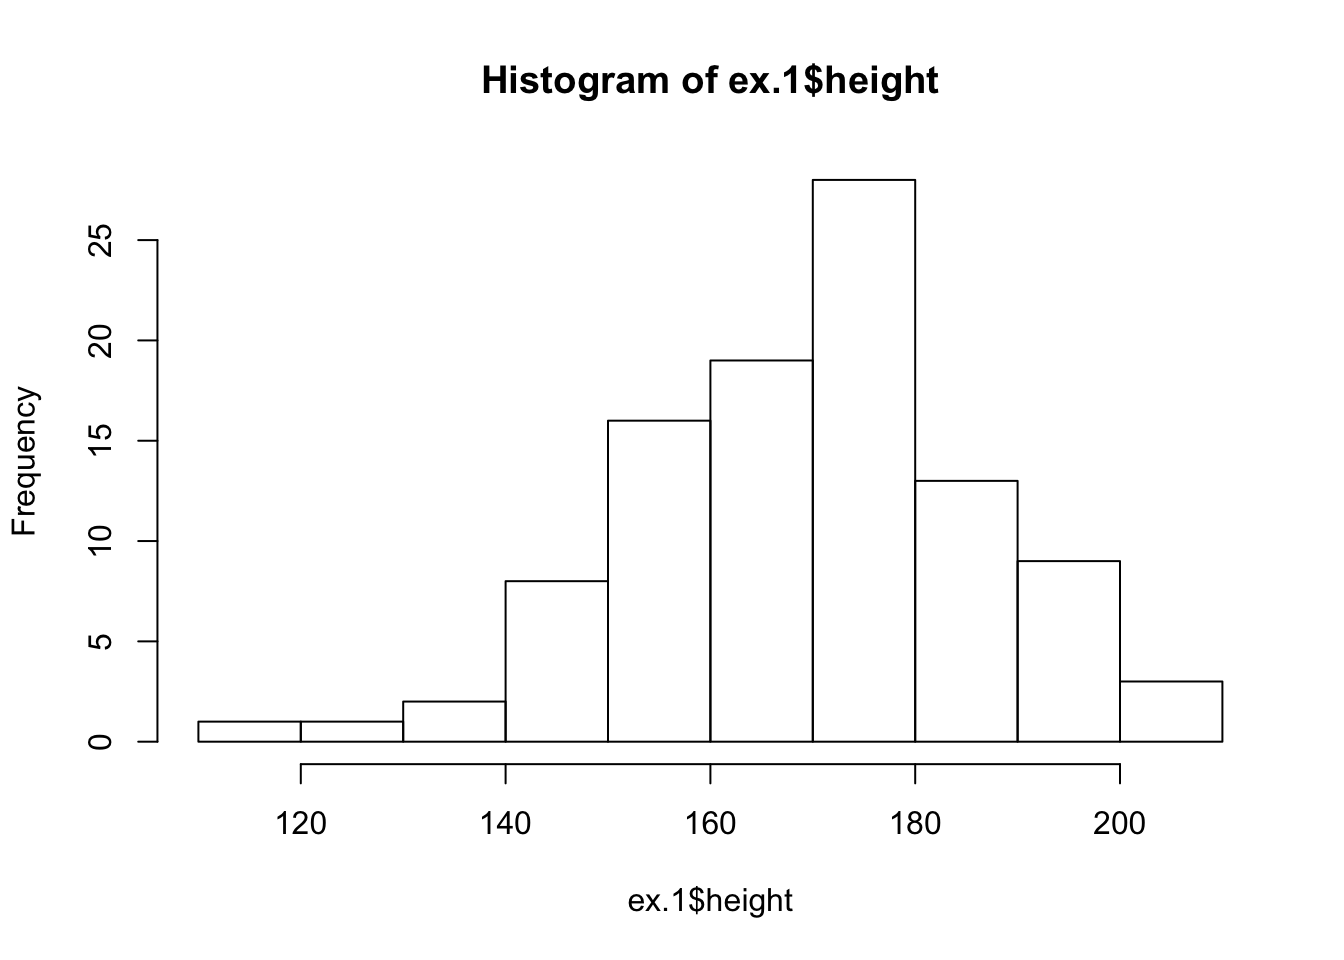
\includegraphics[width=0.6\linewidth]{statthink_files/figure-latex/DStat1-1} 

}

\caption{Histogram of Height}\label{fig:DStat1}
\end{figure}

The data set, which is the content of the CSV file ``\texttt{ex1.csv}'', was used
in Chapter~\ref{ChapData} in order to demonstrate the reading of data that
is stored in a external file into \texttt{R}. The first line of the above
script reads in the data from ``\texttt{ex1.csv}'' into a data frame object named
``\texttt{ex.1}'' that maintains the data internally in \texttt{R}. The second line of
the script produces the histogram. We will discuss below the code
associated with this second line.

A histogram consists of contiguous boxes. It has both a horizontal axis
and a vertical axis. The horizontal axis is labeled with what the data
represents (the height, in this example). The vertical axis presents
frequencies and is labeled ``Frequency''. By the examination of the
histogram one can appreciate the shape of the data, the center, and the
spread of the data.

The histogram is constructed by dividing the range of the data (the
x-axis) into equal intervals, which are the bases for the boxes. The
height of each box represents the count of the number of observations
that fall within the interval. For example, consider the box with the
base between 160 and 170. There is a total of 19 subjects with height
larger that 160 but no more than 170 (that is,
\(160 < \texttt{height} \leq 170\)). Consequently, the height of that
box\footnote{In some books an histogram is introduced as a form of a density.
  In densities the \emph{area} of the box represents the frequency or the
  relative frequency. In the current example the height would have
  been 19/10 = 1.9 if the area of the box would have represented the
  frequency and it would have been \((19/100)/10 = 0.019\) if the area
  of the box would have represented the relative frequency. However,
  in this book we follow the default of \texttt{R} in which the height
  represents the frequency.} is 19.

The input to the function ``\texttt{hist}'' should be a sequence of numerical
values. In principle, one may use the function ``\texttt{c}'' to produce a
sequence of data and apply the histogram plotting function to the output
of the sequence producing function. However, in the current case we have
already the data stored in the data frame ``\texttt{ex.1}'', all we need to learn
is how to extract that data so it can be used as input to the function
``\texttt{hist}'' that plots the histogram.

Notice the structure of the input that we have used in order to
construct the histogram of the variable ``\texttt{height}'' in the ``\texttt{ex.1}'' data
frame. One may address the variable ``\texttt{variable.name}'' in the data frame
``\texttt{dataframe.name}'' using the format: ``\texttt{dataframe.name\$variable.name}''.
Indeed, when we type the expression ``\texttt{ex.1\$height}'' we get as an output
the values of the variable ``\texttt{height}'' from the given data frame:

\begin{Shaded}
\begin{Highlighting}[]
\NormalTok{ex}\FloatTok{.1}\OperatorTok{$}\NormalTok{height}
\end{Highlighting}
\end{Shaded}

\begin{verbatim}
##   [1] 182 168 172 154 174 176 193 156 157 186 143 182 194 187 171 178 157
##  [18] 156 172 157 171 164 142 140 202 176 165 176 175 170 169 153 169 158
##  [35] 208 185 157 147 160 173 164 182 175 165 194 178 178 186 165 180 174
##  [52] 169 173 199 163 160 172 177 165 205 193 158 180 167 165 183 171 191
##  [69] 191 152 148 176 155 156 177 180 186 167 174 171 148 153 136 199 161
##  [86] 150 181 166 147 168 188 170 189 117 174 187 141 195 129 172
\end{verbatim}

This is a numeric sequence and can serve as the input to a function that
expects a numeric sequence as input, a function such as ``\texttt{hist}''. (But
also other functions, for example, ``\texttt{sum}'' and ``\texttt{cumsum}''.)

There are 100 observations in the variable ``\texttt{ex.1\$height}''. So many
observations cannot be displayed on the screen on one line.
Consequently, the sequence of the data is wrapped and displayed over
several lines. Notice that the square brackets on the left hand side of
each line indicate the position in the sequence of the first value on
that line. Hence, the number on the first line is ``\texttt{{[}1{]}}''. The number on
the second line is ``\texttt{{[}16{]}}'', since the second line starts with the 16th
observation in the display given in the book. Notice, that numbers in
the square brackets on your \texttt{R\ Console} window may be different,
depending on the setting of the display on your computer.

\hypertarget{box-plots}{%
\subsection{Box Plots}\label{box-plots}}

The \emph{box plot}, or box-whisker plot, gives a good graphical overall
impression of the concentration of the data. It also shows how far from
most of the data the extreme values are. In principle, the box plot is
constructed from five values: the smallest value, the first quartile,
the median, the third quartile, and the largest value. The median, the
first quartile, and the third quartile will be discussed here, and then
once more in the next section.

The \emph{median}, a number, is a way of measuring the ``center'' of the data.
You can think of the median as the ``middle value,'' although it does not
actually have to be one of the observed values. It is a number that
separates ordered data into halves. Half the values are the same size or
smaller than the median and half the values are the same size or larger
than it. For example, consider the following data that contains 14
values:

\[1,\;   11.5,\;   6,\;   7.2,\;   4,\;   8,\;   9,\;   10,\;   6.8,\;   8.3,\;   2,\;   2,\;   10,\;   1\]
Ordered, from smallest to largest, we get:

\[1,\;   1,\;   2,\;   2,\;   4,\;   6,\;   6.8,\;   7.2,\;   8,\;   8.3,\;   9,\;   10,\;   10,\;   11.5\]

The median is between the 7th value, 6.8, and the 8th value 7.2. To find
the median, add the two values together and divide by 2:

\[\frac{6.8+7.2}{2} = 7\] The median is 7. Half of the values are
smaller than 7 and half of the values are larger than 7.

\emph{Quartiles} are numbers that separate the data into quarters. Quartiles
may or may not be part of the data. To find the quartiles, first find
the median or second quartile. The first quartile is the middle value of
the lower half of the data and the third quartile is the middle value of
the upper half of the data. For illustration consider the same data set
from above:

\[1,\;   1,\;   2,\;   2,\;   4,\;   6,\;   6.8,\;   7.2,\;   8,\;   8.3,\;   9,\;   10,\;   10,\;   11.5\]

The median or second quartile is 7. The lower half of the data is:

\[1,\;   1,\;   2,\;   2,\;   4,\;   6,\;   6.8\] The middle value of
the lower half is 2. The number 2, which is part of the data in this
case, is the first quartile which is denoted Q1. One-fourth of the
values are the same or less than 2 and three-fourths of the values are
more than 2.

The upper half of the data is:

\[7.2,\;   8,\;   8.3,\;   9,\;   10,\;   10,\;   11.5\] The middle
value of the upper half is 9. The number 9 is the third quartile which
is denoted Q3. Three-fourths of the values are less than 9 and
one-fourth of the values\footnote{The actual computation in \texttt{R} of the first quartile and the third
  quartile may vary slightly from the description given here,
  depending on the exact structure of the data.} are more than 9.

\emph{Outliers} are values that do not fit with the rest of the data and lie
outside of the normal range. Data points with values that are much too
large or much too small in comparison to the vast majority of the
observations will be identified as outliers. In the context of the
construction of a box plot we identify potential outliers with the help
of the \emph{inter-quartile range} (IQR). The inter-quartile range is the
distance between the third quartile (Q3) and the first quartile (Q1),
i.e., \(\mbox{IQR} = \mbox{Q3} - \mbox{Q1}\). A data point that is larger
than the third quartile plus 1.5 times the inter-quartile range will be
marked as a potential outlier. Likewise, a data point smaller than the
first quartile minus 1.5 times the inter-quartile range will also be so
marked. Outliers may have a substantial effect on the outcome of
statistical analysis, therefore it is important that one is alerted to
the presence of outliers.

In the running example we obtained an inter-quartile range of size
9-2=7. The upper threshold for defining an outlier is
\(9+1.5 \times 7 = 19.5\) and the lower threshold is
\(2-1.5 \times 7 = -8.5\). All data points are within the two thresholds,
hence there are no outliers in this data.

In the construction of a box plot one uses a vertical rectangular box
and two vertical ``whiskers'' that extend from the ends of the box to the
smallest and largest data values that are not outliers. Outlier values,
if any exist, are marked as points above or blow the endpoints of the
whiskers. The smallest and largest non-outlier data values label the
endpoints of the axis. The first quartile marks one end of the box and
the third quartile marks the other end of the box. The central 50\% of
the data fall within the box.

One may produce a box plot with the aid of the function ``\texttt{boxplot}''. The
input to the function is a sequence of numerical values and the output
is a plot. As an example, let us produce the box plot of the 14 data
points that were used as an illustration:

\begin{Shaded}
\begin{Highlighting}[]
\KeywordTok{boxplot}\NormalTok{(}\KeywordTok{c}\NormalTok{(}\DecValTok{1}\NormalTok{,}\FloatTok{11.5}\NormalTok{,}\DecValTok{6}\NormalTok{,}\FloatTok{7.2}\NormalTok{,}\DecValTok{4}\NormalTok{,}\DecValTok{8}\NormalTok{,}\DecValTok{9}\NormalTok{,}\DecValTok{10}\NormalTok{,}\FloatTok{6.8}\NormalTok{,}\FloatTok{8.3}\NormalTok{,}\DecValTok{2}\NormalTok{,}\DecValTok{2}\NormalTok{,}\DecValTok{10}\NormalTok{,}\DecValTok{1}\NormalTok{))}
\end{Highlighting}
\end{Shaded}

\begin{center}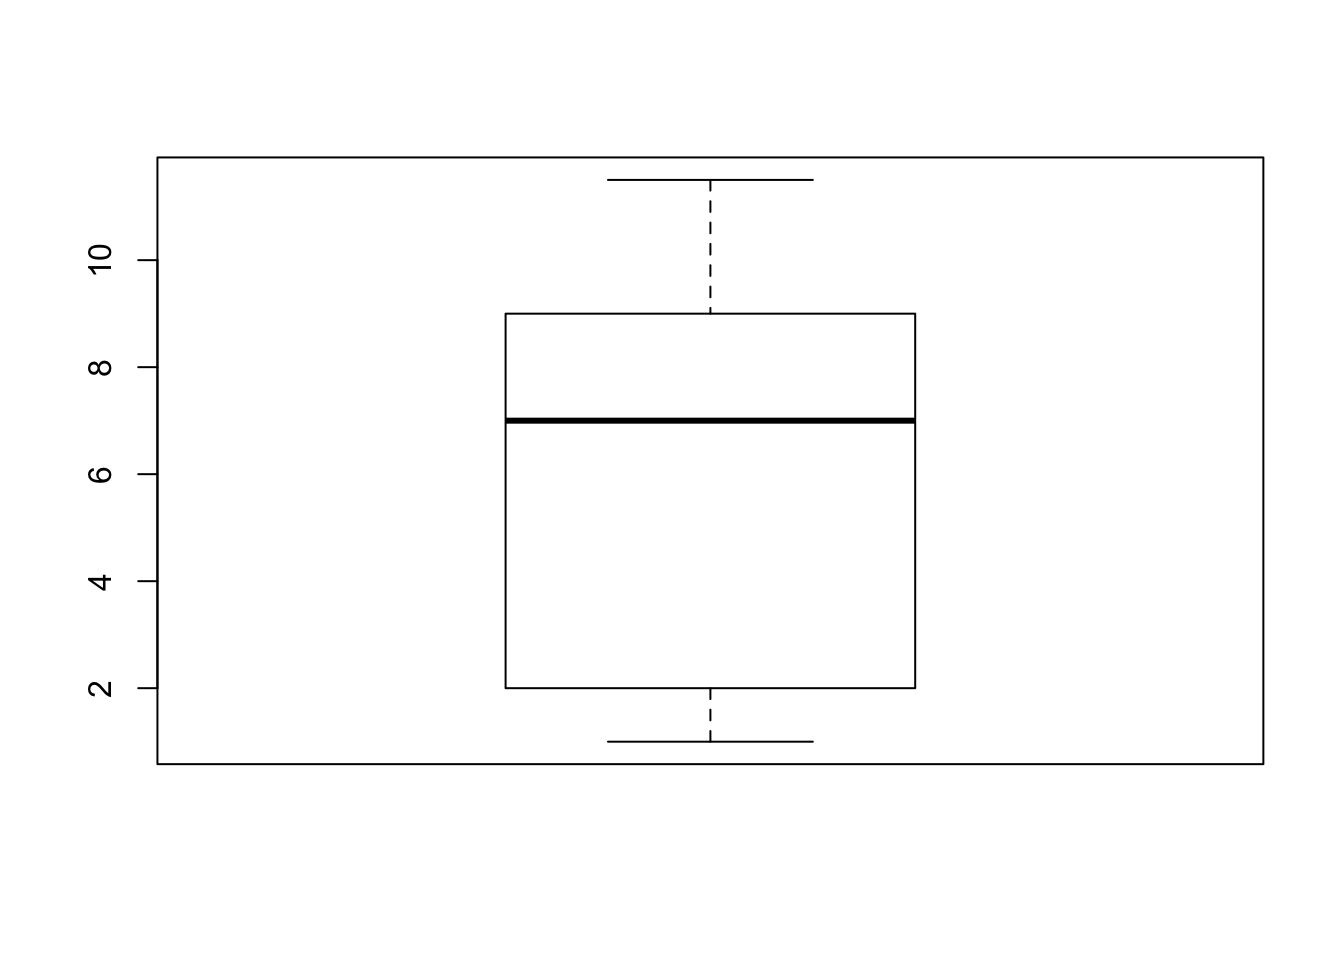
\includegraphics[width=0.6\linewidth]{statthink_files/figure-latex/unnamed-chunk-24-1} \end{center}

Observe that the end points of the
whiskers are 1, for the minimal value, and 11.5 for the largest value.
The end values of the box are 9 for the third quartile and 2 for the
first quartile. The median 7 is marked inside the box.

Next, let us examine the box plot for the height data:

\begin{Shaded}
\begin{Highlighting}[]
\KeywordTok{boxplot}\NormalTok{(ex}\FloatTok{.1}\OperatorTok{$}\NormalTok{height)}
\end{Highlighting}
\end{Shaded}

\begin{center}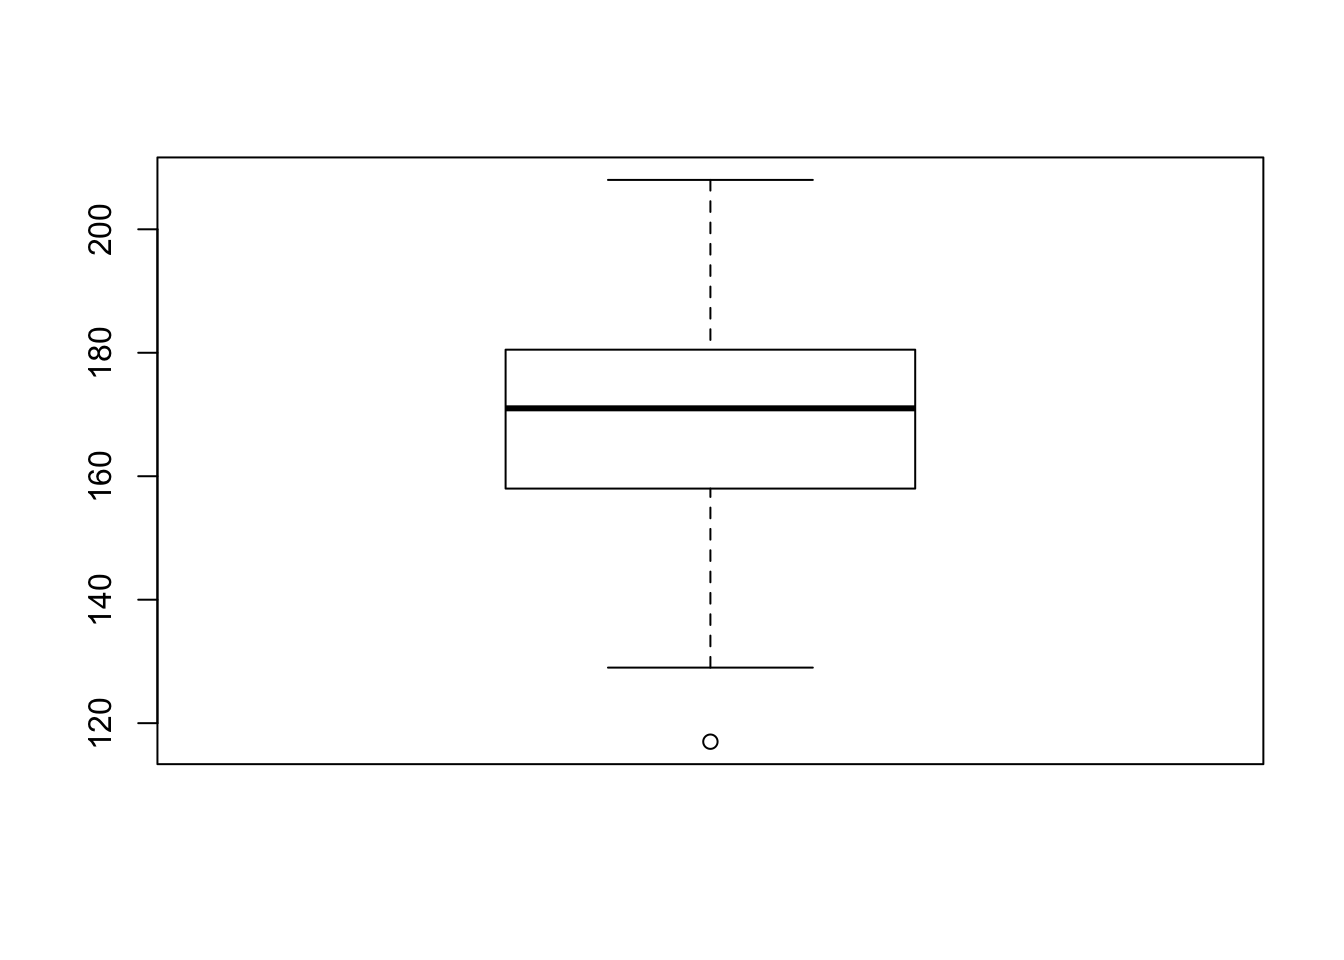
\includegraphics[width=0.6\linewidth]{statthink_files/figure-latex/unnamed-chunk-25-1} \end{center}

In order to assess the plot let us compute quartiles of the variable:

\begin{Shaded}
\begin{Highlighting}[]
\KeywordTok{summary}\NormalTok{(ex}\FloatTok{.1}\OperatorTok{$}\NormalTok{height)}
\end{Highlighting}
\end{Shaded}

\begin{verbatim}
##    Min. 1st Qu.  Median    Mean 3rd Qu.    Max. 
##  117.00  158.00  171.00  170.11  180.25  208.00
\end{verbatim}

The function ``\texttt{summary}'', when applied to a numerical sequence, produce
the minimal and maximal entries, as well the first, second and third
quartiles (the second is the Median). It also computes the average of
the numbers (the Mean), which will be discussed in the next section.

Let us compare the results with the box plot for the height data.
Observe that the median 171 coincides
with the thick horizontal line inside the box and that the lower end of
the box coincides with first quartile 158.0 and the upper end with
180.2, which is the third quartile. The inter-quartile range is
\(180.2 - 158.0 = 22.2\). The upper threshold is
\(180.2 + 1.5 \times 22.2 = 213.5\). This threshold is larger than the
largest observation (208.0). Hence, the largest observation is not an
outlier and it marks the end of the upper whisker. The lower threshold
is \(158.0 - 1.5 \times 22.2 = 124.7\). The minimal observation (117.0) is
less than this threshold. Hence it is an outlier and it is marked as a
point below the end of the lower whisker. The second smallest
observation is 129. It lies above the lower threshold and it marks the
end point of the lower whisker.

\hypertarget{measures-of-the-center-of-data}{%
\section{Measures of the Center of Data}\label{measures-of-the-center-of-data}}

The two most widely used measures of the central location of the data
are the \emph{mean} (average) and the \emph{median}. To calculate the average
weight of 50 people one should add together the 50 weights and divide
the result by 50. To find the median weight of the same 50 people, one
may order the data and locate a number that splits the data into two
equal parts. The median is generally a better measure of the center when
there are extreme values or outliers because it is not affected by the
precise numerical values of the outliers. Nonetheless, the mean is the
most commonly used measure of the center.

We shall use small Latin letters such as \(x\) to mark the sequence of
data. In such a case we may mark the sample mean by placing a bar over
the \(x\): \(\bar x\) (pronounced ``\(x\) bar'').

The mean can be calculated by averaging the data points or it also can
be calculated with the relative frequencies of the values that are
present in the data. In the latter case one multiplies each distinct
value by its relative frequency and then sum the products across all
values. To see that both ways of calculating the mean are the same,
consider the data:

\[1,\; 1,\; 1,\; 2,\; 2,\; 3,\; 4,\; 4,\; 4,\; 4,\; 4\] In the first
way of calculating the mean we get:

\[\bar x = \frac{1 + 1 + 1 + 2 + 2 + 3 + 4 + 4 + 4 + 4 + 4}{11} = 2.7\;.\]

Alternatively, we may note that the distinct values in the sample are 1,
2, 3, and 4 with relative frequencies of 3/11, 2/11, 1/11 and 5/11,
respectively. The alternative method of computation produces:

\[\bar x = 1\times \frac{3}{11} + 2 \times \frac{2}{11} + 3 \times \frac{1}{11} + 4 \times \frac{5}{11} = 2.7\;.\]

\hypertarget{skewness-the-mean-and-the-median}{%
\subsection{Skewness, the Mean and the Median}\label{skewness-the-mean-and-the-median}}

\begin{figure}

{\centering 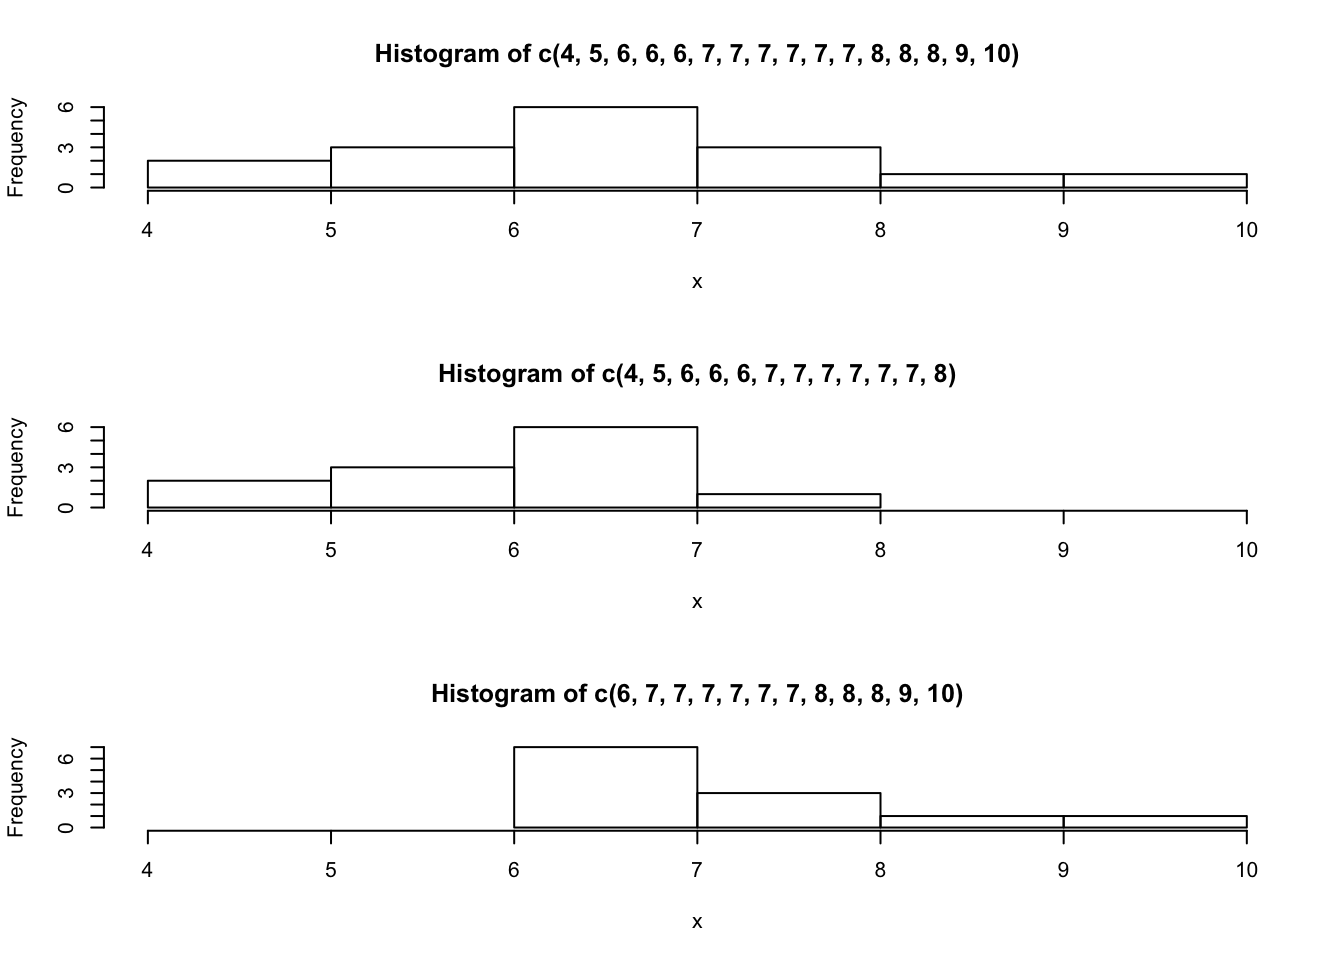
\includegraphics[width=0.6\linewidth]{statthink_files/figure-latex/DStat4-1} 

}

\caption{Three Histograms}\label{fig:DStat4}
\end{figure}

Consider the following data set:

\[4,\; 5,\; 6,\; 6,\; 6,\; 7,\; 7,\; 7,\; 7,\;  7,\;  7,\;  8,\;  8,\;  8,\;  9,\;  10\]
This data produces the upper most histogram in
Figure~\ref{fig:DStat4}. Each interval has width one and each
value is located at the middle of an interval. The histogram displays a
symmetrical distribution of data. A distribution is symmetrical if a
vertical line can be drawn at some point in the histogram such that the
shape to the left and to the right of the vertical line are mirror
images of each other.

Let us compute the mean and the median of this data:

\begin{Shaded}
\begin{Highlighting}[]
\NormalTok{x <-}\StringTok{ }\KeywordTok{c}\NormalTok{(}\DecValTok{4}\NormalTok{,}\DecValTok{5}\NormalTok{,}\DecValTok{6}\NormalTok{,}\DecValTok{6}\NormalTok{,}\DecValTok{6}\NormalTok{,}\DecValTok{7}\NormalTok{,}\DecValTok{7}\NormalTok{,}\DecValTok{7}\NormalTok{,}\DecValTok{7}\NormalTok{,}\DecValTok{7}\NormalTok{,}\DecValTok{7}\NormalTok{,}\DecValTok{8}\NormalTok{,}\DecValTok{8}\NormalTok{,}\DecValTok{8}\NormalTok{,}\DecValTok{9}\NormalTok{,}\DecValTok{10}\NormalTok{)}
\KeywordTok{mean}\NormalTok{(x)}
\end{Highlighting}
\end{Shaded}

\begin{verbatim}
## [1] 7
\end{verbatim}

\begin{Shaded}
\begin{Highlighting}[]
\KeywordTok{median}\NormalTok{(x)}
\end{Highlighting}
\end{Shaded}

\begin{verbatim}
## [1] 7
\end{verbatim}

The mean and the median are each 7 for these data. In a perfectly
symmetrical distribution, the mean and the median are the same\footnote{In the case of a symmetric distribution the vertical line of
  symmetry is located at the mean, which is also equal to the median.}.

The functions ``\texttt{mean}'' and ``\texttt{median}'' were used in order to compute the
mean and median. Both functions expect a numeric sequence as an input
and produce the appropriate measure of centrality of the sequence as an
output.

The histogram for the data:

\[4,\;  5,\;  6,\;  6,\;  6,\;  7,\;  7,\;  7,\;  7,\;  7,\;  7,\;  8\]
is not symmetrical and is displayed in the middle of
Figure~\ref{fig:DStat4}. The right-hand side seems ``chopped
off'' compared to the left side. The shape of the distribution is called
skewed to the left because it is pulled out towards the left.

Let us compute the mean and the median for this data:

\begin{Shaded}
\begin{Highlighting}[]
\NormalTok{x <-}\StringTok{ }\KeywordTok{c}\NormalTok{(}\DecValTok{4}\NormalTok{,}\DecValTok{5}\NormalTok{,}\DecValTok{6}\NormalTok{,}\DecValTok{6}\NormalTok{,}\DecValTok{6}\NormalTok{,}\DecValTok{7}\NormalTok{,}\DecValTok{7}\NormalTok{,}\DecValTok{7}\NormalTok{,}\DecValTok{7}\NormalTok{,}\DecValTok{7}\NormalTok{,}\DecValTok{7}\NormalTok{,}\DecValTok{8}\NormalTok{)}
\KeywordTok{mean}\NormalTok{(x)}
\end{Highlighting}
\end{Shaded}

\begin{verbatim}
## [1] 6.4166667
\end{verbatim}

\begin{Shaded}
\begin{Highlighting}[]
\KeywordTok{median}\NormalTok{(x)}
\end{Highlighting}
\end{Shaded}

\begin{verbatim}
## [1] 7
\end{verbatim}

(Notice that the original data is replaced by the new data when object
\texttt{x} is reassigned.) The median is still 7, but the mean is less than 7.
The relation between the mean and the median reflects the skewing.

Consider yet another set of data:

\[6,\;  7,\;  7,\;  7,\;  7,\;  7,\;  7,\;  8,\;  8,\;  8,\;  9,\;  10\]
The histogram for the data is also not symmetrical and is displayed at
the bottom of Figure~\ref{fig:DStat4}. Notice that it is
skewed to the right. Compute the mean and the median:

\begin{Shaded}
\begin{Highlighting}[]
\NormalTok{x <-}\StringTok{ }\KeywordTok{c}\NormalTok{(}\DecValTok{6}\NormalTok{,}\DecValTok{7}\NormalTok{,}\DecValTok{7}\NormalTok{,}\DecValTok{7}\NormalTok{,}\DecValTok{7}\NormalTok{,}\DecValTok{7}\NormalTok{,}\DecValTok{7}\NormalTok{,}\DecValTok{8}\NormalTok{,}\DecValTok{8}\NormalTok{,}\DecValTok{8}\NormalTok{,}\DecValTok{9}\NormalTok{,}\DecValTok{10}\NormalTok{)}
\KeywordTok{mean}\NormalTok{(x)}
\end{Highlighting}
\end{Shaded}

\begin{verbatim}
## [1] 7.5833333
\end{verbatim}

\begin{Shaded}
\begin{Highlighting}[]
\KeywordTok{median}\NormalTok{(x)}
\end{Highlighting}
\end{Shaded}

\begin{verbatim}
## [1] 7
\end{verbatim}

The median is yet again equal to 7, but this time the mean is greater
than 7. Again, the mean reflects the skewing.

In summary, if the distribution of data is skewed to the left then the
mean is less than the median. If the distribution of data is skewed to
the right then the median is less than the mean.

Examine the data on the height in ``\texttt{ex.1}'':

\begin{Shaded}
\begin{Highlighting}[]
\KeywordTok{mean}\NormalTok{(ex}\FloatTok{.1}\OperatorTok{$}\NormalTok{height)}
\end{Highlighting}
\end{Shaded}

\begin{verbatim}
## [1] 170.11
\end{verbatim}

\begin{Shaded}
\begin{Highlighting}[]
\KeywordTok{median}\NormalTok{(ex}\FloatTok{.1}\OperatorTok{$}\NormalTok{height)}
\end{Highlighting}
\end{Shaded}

\begin{verbatim}
## [1] 171
\end{verbatim}

Observe that the histogram of the height
(Figure~\ref{fig:DStat1}) is skewed to the left. This is
consistent with the fact that the mean is less than the median.

\hypertarget{measures-of-the-spread-of-data}{%
\section{Measures of the Spread of Data}\label{measures-of-the-spread-of-data}}

One measure of the spread of the data is the inter-quartile range that
was introduced in the context of the box plot. However, the most
important measure of spread is the standard deviation.

Before dealing with the standard deviation let us discuss the
calculation of the variance. If \(x_i\) is a data value for subject \(i\)
and \(\bar x\) is the sample mean, then \(x_i-\bar x\) is called the
deviation of subject \(i\) from the mean, or simply the deviation. In a
data set, there are as many deviations as there are data values. The
variance is in principle the average of the squares of the deviations.

Consider the following example: In a fifth grade class, the teacher was
interested in the average age and the standard deviation of the ages of
her students. Here are the ages of her students to the nearest half a
year:

\[\begin{aligned}
& 9,\; 9.5,\; 9.5,\; 10,\; 10,\; 10,\; 10,\; 10.5,\; 10.5,\; 10.5,\; 10.5,\; 11,\; 11,\; 11,\; 11,\; 11,\; 11,\;\\
& 11.5,\; 11.5,\; 11.5\;.\end{aligned}\]

In order to explain the computation of the variance of these data let us
create an object \texttt{x} that contains the data:

\begin{Shaded}
\begin{Highlighting}[]
\NormalTok{x <-}\StringTok{ }\KeywordTok{c}\NormalTok{(}\DecValTok{9}\NormalTok{,}\FloatTok{9.5}\NormalTok{,}\FloatTok{9.5}\NormalTok{,}\DecValTok{10}\NormalTok{,}\DecValTok{10}\NormalTok{,}\DecValTok{10}\NormalTok{,}\DecValTok{10}\NormalTok{,}\FloatTok{10.5}\NormalTok{,}\FloatTok{10.5}\NormalTok{,}\FloatTok{10.5}\NormalTok{,}\FloatTok{10.5}\NormalTok{,}\DecValTok{11}\NormalTok{,}\DecValTok{11}\NormalTok{,}\DecValTok{11}\NormalTok{,}\DecValTok{11}\NormalTok{,}\DecValTok{11}\NormalTok{,}\DecValTok{11}\NormalTok{,}\FloatTok{11.5}\NormalTok{,}\FloatTok{11.5}\NormalTok{,}\FloatTok{11.5}\NormalTok{)}
\KeywordTok{length}\NormalTok{(x)}
\end{Highlighting}
\end{Shaded}

\begin{verbatim}
## [1] 20
\end{verbatim}

Pay attention to the fact that we did not write the ``\texttt{+}'' at the
beginning of the second line. That symbol was produced by \texttt{R} when
moving to the next line to indicate that the expression is not complete
yet and will not be executed. Only after inputting the right bracket and
the hitting of the Return key does \texttt{R} carry out the command and creates
the object ``\texttt{x}''. When you execute this example yourself on your own
computer make sure not to copy the ``\texttt{+}'' sign. Instead, if you hit the
return key after the last comma on the first line, the plus sign will be
produced by \texttt{R} as a new prompt and you can go on typing in the rest of
the numbers.

The function ``\texttt{length}'' returns the length of the input sequence. Notice
that we have a total of 20 data points.

The next step involves the computation of the deviations:

\begin{Shaded}
\begin{Highlighting}[]
\NormalTok{x.bar <-}\StringTok{ }\KeywordTok{mean}\NormalTok{(x)}
\NormalTok{x.bar}
\end{Highlighting}
\end{Shaded}

\begin{verbatim}
## [1] 10.525
\end{verbatim}

\begin{Shaded}
\begin{Highlighting}[]
\NormalTok{x }\OperatorTok{-}\StringTok{ }\NormalTok{x.bar}
\end{Highlighting}
\end{Shaded}

\begin{verbatim}
##  [1] -1.525 -1.025 -1.025 -0.525 -0.525 -0.525 -0.525 -0.025 -0.025 -0.025
## [11] -0.025  0.475  0.475  0.475  0.475  0.475  0.475  0.975  0.975  0.975
\end{verbatim}

The average of the observations is equal to 10.525 and when we delete
this number from each of the components of the sequence \texttt{x} we obtain
the deviations. For example, the first deviation is obtained as 9 -
10.525 = -1.525, the second deviation is 9.5 - 10.525 = -1.025, and so
forth. The 20th deviation is 11.5 - 10.525 = 0.975, and this is the last
number that is presented in the output.

From a more technical point of view observe that the expression that
computed the deviations, ``\texttt{x\ -\ x.bar}'', involved the deletion of a
single value (\texttt{x.bar}) from a sequence with 20 values (\texttt{x}). The
expression resulted in the deletion of the value from each component of
the sequence. This is an example of the general way by which \texttt{R}
operates on sequences. The typical behavior of \texttt{R} is to apply an
operation to each component of the sequence.

As yet another illustration of this property consider the computation of
the squares of the deviations:

\begin{Shaded}
\begin{Highlighting}[]
\NormalTok{(x }\OperatorTok{-}\StringTok{ }\NormalTok{x.bar)}\OperatorTok{^}\DecValTok{2}
\end{Highlighting}
\end{Shaded}

\begin{verbatim}
##  [1] 2.325625 1.050625 1.050625 0.275625 0.275625 0.275625 0.275625
##  [8] 0.000625 0.000625 0.000625 0.000625 0.225625 0.225625 0.225625
## [15] 0.225625 0.225625 0.225625 0.950625 0.950625 0.950625
\end{verbatim}

Recall that ``\texttt{x\ -\ x.bar}'' is a sequence of length 20. We apply the
square function to this sequence. This function is applied to each of
the components of the sequence. Indeed, for the first component we have
that \((-1.525)^2 = 2.325625\), for the second component
\((-1.025)^2 = 1.050625\), and for the last component
\((0.975)^2 = 0.950625\).

For the variance we sum the square of the deviations and divide by the
total number of data values minus one (\(n-1\)). The standard deviation is
obtained by taking the square root of the variance:

\begin{Shaded}
\begin{Highlighting}[]
\KeywordTok{sum}\NormalTok{((x }\OperatorTok{-}\StringTok{ }\NormalTok{x.bar)}\OperatorTok{^}\DecValTok{2}\NormalTok{)}\OperatorTok{/}\NormalTok{(}\KeywordTok{length}\NormalTok{(x)}\OperatorTok{-}\DecValTok{1}\NormalTok{)}
\end{Highlighting}
\end{Shaded}

\begin{verbatim}
## [1] 0.5125
\end{verbatim}

\begin{Shaded}
\begin{Highlighting}[]
\KeywordTok{sqrt}\NormalTok{(}\KeywordTok{sum}\NormalTok{((x }\OperatorTok{-}\StringTok{ }\NormalTok{x.bar)}\OperatorTok{^}\DecValTok{2}\NormalTok{)}\OperatorTok{/}\NormalTok{(}\KeywordTok{length}\NormalTok{(x)}\OperatorTok{-}\DecValTok{1}\NormalTok{))}
\end{Highlighting}
\end{Shaded}

\begin{verbatim}
## [1] 0.71589105
\end{verbatim}

If the variance is produced as a result of dividing the sum of squares
by the number of observations minus one then the variance is called the
\emph{sample variance}.

The function ``\texttt{var}'' computes the sample variance and the function
``\texttt{sd}'' computes the standard deviations. The input to both functions is
the sequence of data values and the outputs are the sample variance and
the standard deviation, respectively:

\begin{Shaded}
\begin{Highlighting}[]
\KeywordTok{var}\NormalTok{(x)}
\end{Highlighting}
\end{Shaded}

\begin{verbatim}
## [1] 0.5125
\end{verbatim}

\begin{Shaded}
\begin{Highlighting}[]
\KeywordTok{sd}\NormalTok{(x)}
\end{Highlighting}
\end{Shaded}

\begin{verbatim}
## [1] 0.71589105
\end{verbatim}

In the computation of the variance we divide the sum of squared
deviations by the number of deviations minus one and not by the number
of deviations. The reason for that stems from the theory of statistical
inference that will be discussed in Part II of this book. Unless the
size of the data is small, dividing by \(n\) or by \(n-1\) does not
introduce much of a difference.

The variance is a squared measure and does not have the same units as
the data. Taking the square root solves the problem. The standard
deviation measures the spread in the same units as the data.

The sample standard deviation, \(s\), is either zero or is larger than
zero. When \(s=0\), there is no spread and the data values are equal to
each other. When \(s\) is a lot larger than zero, the data values are very
spread out about the mean. Outliers can make \(s\) very large.

The standard deviation is a number that measures how far data values are
from their mean. For example, if the data contains the value 7 and if
the mean of the data is 5 and the standard deviation is 2, then the
value 7 is one standard deviation from its mean because
\(5 + 1 \times 2 = 7\). We say, then, that 7 is one standard deviation
larger than the mean 5 (or also say ``to the right of 5''). If the value 1
was also part of the data set, then 1 is two standard deviations smaller
than the mean (or two standard deviations to the left of 5) because
\(5 - 2 \times 2 = 1\).

The standard deviation, when first presented, may not be too simple to
interpret. By graphing your data, you can get a better ``feel'' for the
deviations and the standard deviation. You will find that in symmetrical
distributions, the standard deviation can be very helpful but in skewed
distributions, the standard deviation is less so. The reason is that the
two sides of a skewed distribution have different spreads. In a skewed
distribution, it is better to look at the first quartile, the median,
the third quartile, the smallest value, and the largest value.

\hypertarget{exercises-2}{%
\section{Exercises}\label{exercises-2}}

\BeginKnitrBlock{exercise}
\protect\hypertarget{exr:unnamed-chunk-36}{}{\label{exr:unnamed-chunk-36} }Three sequences of data were saved in 3 \texttt{R}
objects named ``\texttt{x1}'', ``\texttt{x2}'' and ``\texttt{x3}'', respectively. The application
of the function ``\texttt{summary}'' to each of these objects is presented below:

\begin{verbatim}
> summary(x1)
   Min. 1st Qu.  Median    Mean 3rd Qu.    Max.
  0.000   2.498   3.218   3.081   3.840   4.871
> summary(x2)
     Min.   1st Qu.    Median      Mean   3rd Qu.      Max.
0.0001083 0.5772000 1.5070000 1.8420000 2.9050000 4.9880000
> summary(x3)
   Min. 1st Qu.  Median    Mean 3rd Qu.    Max.
  2.200   3.391   4.020   4.077   4.690   6.414
\end{verbatim}

In Figure~\ref{fig:DStat9} one may find the histograms of
these three data sequences, given in a random order. In
Figure~\ref{fig:DStat10} one may find the box plots of the
same data, given in yet a different order.

\begin{enumerate}
\def\labelenumi{\arabic{enumi}.}
\item
  Match the summary result with the appropriate histogram and the
  appropriate box plot.
\item
  Is the value 0.000 in the sequence ``\texttt{x1}'' an outlier?
\item
  Is the value 6.414 in the sequence ``\texttt{x3}'' an outlier?
\end{enumerate}
\EndKnitrBlock{exercise}

\begin{figure}
\centering
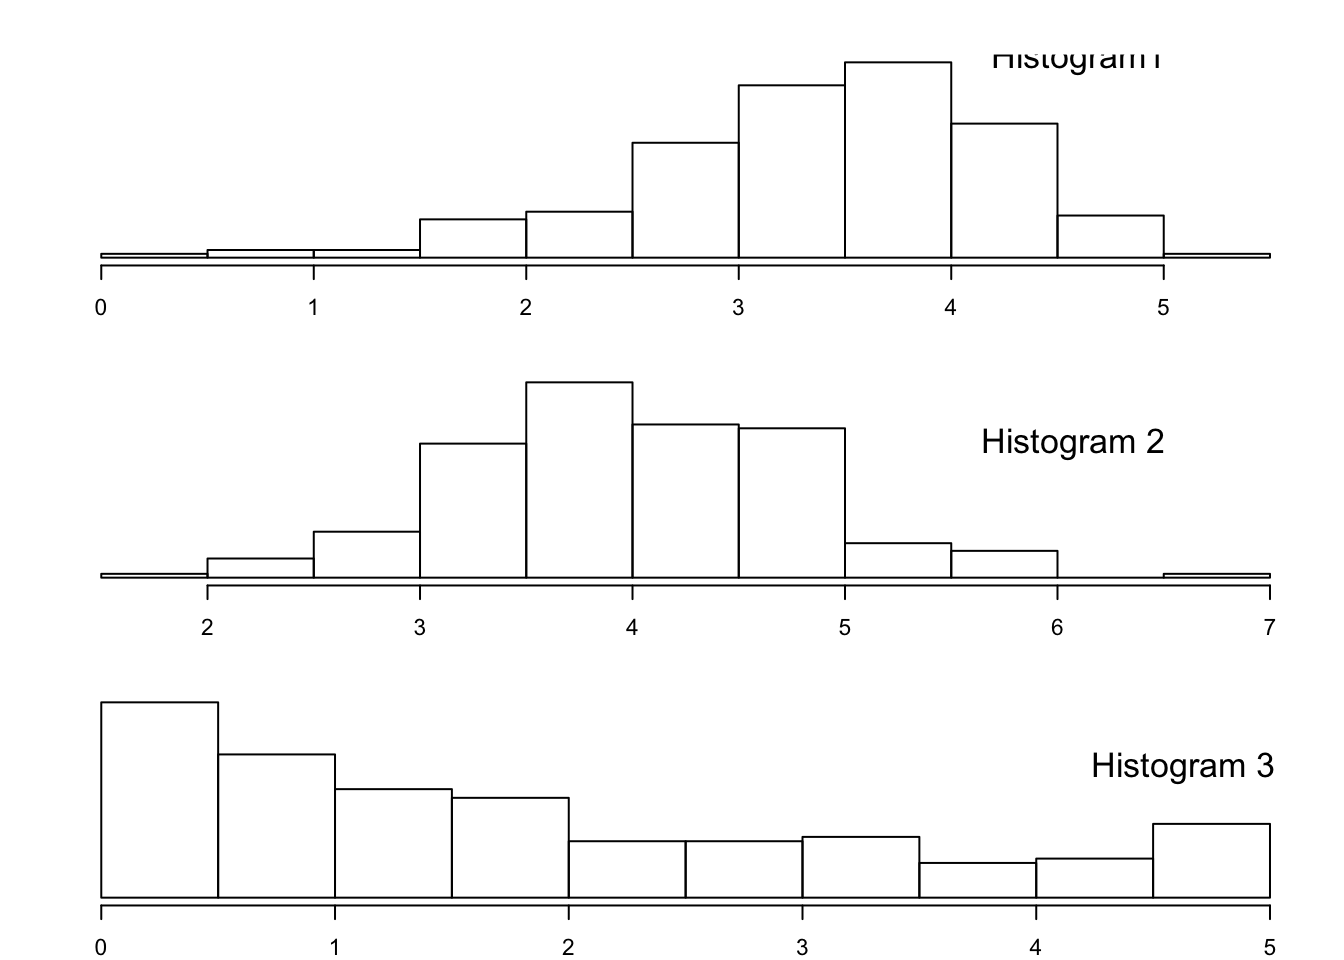
\includegraphics{statthink_files/figure-latex/DStat9-1.pdf}
\caption{\label{fig:DStat9}Three Histograms}
\end{figure}

\begin{figure}
\centering
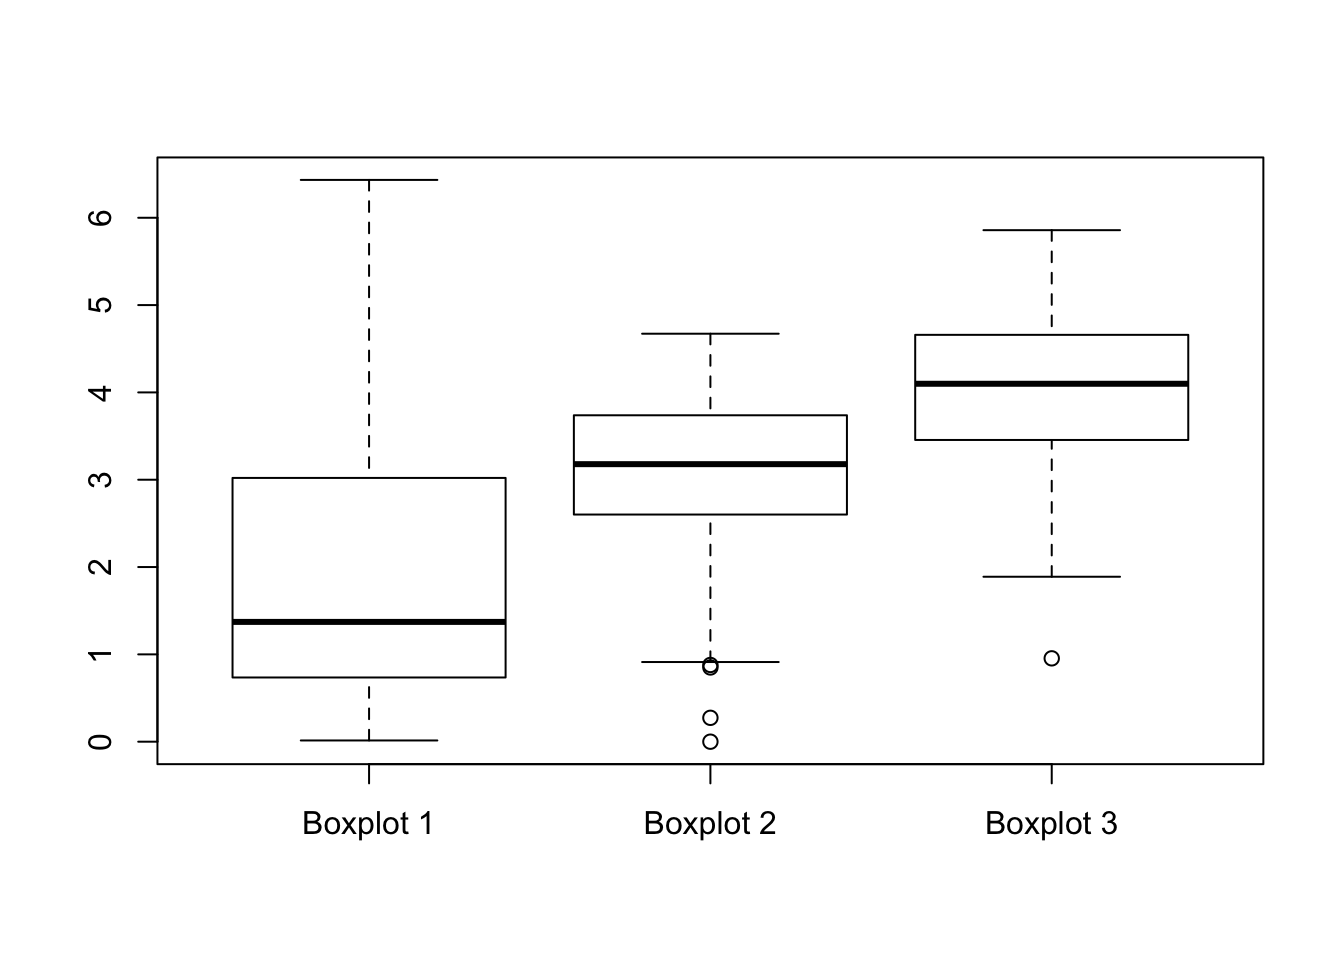
\includegraphics{statthink_files/figure-latex/DStat10-1.pdf}
\caption{\label{fig:DStat10}Three Box Plots}
\end{figure}

\BeginKnitrBlock{exercise}
\protect\hypertarget{exr:unnamed-chunk-38}{}{\label{exr:unnamed-chunk-38} }The number of toilet facilities in 30 buildings
were counted. The results are recorded in an \texttt{R} object by the name
``\texttt{x}''. The frequency table of the data ``\texttt{x}'' is:

\begin{verbatim}
> table(x)
x
 2  4  6  8 10
10  6 10  2  2
\end{verbatim}

\begin{enumerate}
\def\labelenumi{\arabic{enumi}.}
\item
  What is the mean (\(\bar x\)) of the data?
\item
  What is the sample standard deviation of the data?
\item
  What is the median of the data?
\item
  What is the inter-quartile range (IQR) of the data?
\item
  How many standard deviations away from the mean is the value 10?
\end{enumerate}
\EndKnitrBlock{exercise}

\hypertarget{summary-2}{%
\section{Summary}\label{summary-2}}

\hypertarget{glossary}{%
\subsection*{Glossary}\label{glossary}}


\begin{description}
\item[Median:]
A number that separates ordered data into halves: half the values
are the same number or smaller than the median and half the values
are the same number or larger than the median. The median may or may
not be part of the data.
\item[Quartiles:]
The numbers that separate the data into quarters. Quartiles may or
may not be part of the data. The second quartile is the median of
the data.
\item[Outlier:]
An observation that does not fit the rest of the data.
\item[Interquartile Range (IQR)]
: The distance between the third quartile (Q3) and the first
quartile (Q1). IQR = Q3 - Q1.
\item[Mean:]
A number that measures the central tendency. A common name for mean
is `average.' The term `mean' is a shortened form of `arithmetic
mean.' By definition, the mean for a sample (denoted by \(\bar x\)) is

\[\bar x = \frac{\mbox{Sum of all values in the sample}}{\mbox{Number of values in the sample}}\;.\]
\item[(Sample) Variance:]
Mean of the squared deviations from the mean. Square of the standard
deviation. For a set of data, a deviation can be represented as
\(x - \bar x\) where \(x\) is a value of the data and \(\bar x\) is the
sample mean. The sample variance is equal to the sum of the squares
of the deviations divided by the difference of the sample size and
1:

\[s^2 = \frac{\mbox{Sum of the squares of the deviations}}{\mbox{Number of values in the sample}-1}\;.\]
\item[(Sample) Standard Deviation:]
A number that is equal to the square root of the variance and
measures how far data values are from their mean. \(s = \sqrt{s^2}\).
\end{description}

\hypertarget{discuss-in-the-forum}{%
\subsection*{Discuss in the forum}\label{discuss-in-the-forum}}


An important practice is to check the validity of any data set that you
are supposed to analyze in order to detect errors in the data and
outlier observations. Recall that outliers are observations with values
outside the normal range of values of the rest of the observations.

It is said by some that outliers can help us understand our data better.
What is your opinion?

When forming your answer to this question you may give an example of how
outliers may provide insight or, else, how they may abstract our
understanding. For example, consider the price of a stock that tend to
go up or go down at most 2\% within each trading day. A sudden 5\% drop in
the price of the stock may be an indication to reconsidering our
position with respect to this stock.

\hypertarget{commonly-used-symbols}{%
\subsection*{Commonly Used Symbols}\label{commonly-used-symbols}}


\begin{itemize}
\item
  The symbol \(\sum\) means to add or to find the sum.
\item
  \(n\) = the number of data values in a sample.
\item
  \(\bar x\) = the sample mean.
\item
  \(s\) = the sample standard deviation.
\item
  \(f\) = frequency.
\item
  \(f/n\) = relative frequency.
\item
  \(x\) = numerical value.
\end{itemize}

\hypertarget{commonly-used-expressions}{%
\subsection*{Commonly Used Expressions}\label{commonly-used-expressions}}


\begin{itemize}
\item
  \(x \times (f_x/n)\) = A value multiplied by its respective relative
  frequency.
\item
  \(\sum_{i=1}^n x_i\) = The sum of the data values.
\item
  \(\sum_x (x \times f_x/n)\)= The sum of values multiplied by their
  respective relative frequencies.
\item
  \(x - \bar x\) = Deviations from the mean (how far a value is from the
  mean).
\item
  \((x - \bar x)^2\) = Deviations squared.
\end{itemize}

\hypertarget{formulas}{%
\subsection*{Formulas:}\label{formulas}}


\begin{itemize}
\item
  Mean:
  \(\bar x = \frac{1}{n} \sum_{i=1}^n x_i = \sum_x \big(x \times (f_x/n)\big)\)
\item
  Variance:
  \(s^2 = \frac{1}{n-1}\sum_{i=1}^n (x_i - \bar x)^2 = \frac{n}{n-1}\sum_x \big((x - \bar x)^2\times (f_x/n)\big)\)
\item
  Standard Deviation: \(s = \sqrt{s^2}\)
\end{itemize}

\hypertarget{ChapProbability}{%
\chapter{Probability}\label{ChapProbability}}

\hypertarget{student-learning-objective}{%
\section{Student Learning Objective}\label{student-learning-objective}}

This section extends the notion of variability that was introduced in
the context of data to other situations. The variability of the entire
\emph{population} and the concept of a \emph{random variable} is discussed. These
concepts are central for the development and interpretation of
statistical inference. By the end of the chapter the student should:

\begin{itemize}
\item
  Consider the distribution of a variable in a population and compute
  parameters of this distribution, such as the mean and the standard
  deviation.
\item
  Become familiar with the concept of a random variable.
\item
  Understand the relation between the distribution of the population
  and the distribution of a random variable produced by sampling a
  random subject from the population.
\item
  Identify the distribution of the random variable in simple settings
  and compute its expectation and variance.
\end{itemize}

\hypertarget{different-forms-of-variability}{%
\section{Different Forms of Variability}\label{different-forms-of-variability}}

In the previous chapters we examined the variability in data. In the
statistical context, data is obtained by selecting a sample from the
target population and measuring the quantities of interest for the
subjects that belong to the sample. Different subjects in the sample may
obtain different values for the measurement, leading to variability in
the data.

This variability may be summarized with the aid of a \emph{frequency table},
a table of \emph{relative frequency}, or via the \emph{cumulative relative
frequency}. A graphical display of the variability in the data may be
obtained with the aid of the \emph{bar plot}, the \emph{histogram}, or the \emph{box
plot}.

Numerical summaries may be computed in order to characterize the main
features of the variability. We used the \emph{mean} and the \emph{median} in
order to identify the location of the distribution. The \emph{sample
variance}, or better yet the \emph{sample standard deviation}, as well as the
\emph{inter-quartile range} were all described as tools to quantify the
overall spread of the data.

The aim of all these graphical representations and numerical summaries
is to investigate the variability of the data.

The subject of this chapter is to introduce two other forms of
variability, variability that is not associated, at least not directly,
with the data that we observe. The first type of variability is the
\emph{population variability}. The other type of variability is the
variability of a \emph{random variable}.

The notions of variability that will be presented are abstract, they are
not given in terms of the data that we observe, and they have a
mathematical-theoretical flavor to them. At first, these abstract
notions may look to you as a waste of your time and may seem to be
unrelated to the subject matter of the course. The opposite is true. The
very core of statistical thinking is relating observed data to
theoretical and abstract models of a phenomena. Via this comparison, and
using the tools of statistical inference that are presented in the
second half of the book, statisticians can extrapolate insights or make
statements regarding the phenomena on the basis of the observed data.
Thereby, the abstract notions of variability that are introduced in this
chapter, and are extended in the subsequent chapters up to the end of
this part of the book, are the essential foundations for the practice of
statistics.

The first notion of variability is the variability that is associated
with the population. It is similar in its nature to the variability of
the data. The difference between these two types of variability is that
the former corresponds to the variability of the quantity of interest
across all members of the population and not only for those that were
selected to the sample.

In Chapters~\ref{ChapData} and~\ref{ChapDescriptiveStat} we examined the data
set ``\texttt{ex.1}'' which contained data on the sex and height of a sample of
100 observations. In this chapter we will consider the sex and height of
\emph{all} the members of the population from which the sample was selected.
The size of the relevant population is 100,000, including the 100
subjects that composed the sample. When we examine the values of the
height across the entire population we can see that different people may
have different heights. This variability of the heights is the
population variability.

The other abstract type of variability, the variability of a random
variable, is a mathematical concept. The aim of this concept is to model
the notion of randomness in measurements or the uncertainty regarding
the outcome of a measurement. In particular we will initially consider
the variability of a random variable in the context of selecting one
subject at random from the population.

Imagine we have a population of size 100,000 and we are about to select
at random one subject from this population. We intend to measure the
height of the subject that will be selected. Prior to the selection and
measurement we are not certain what value of height will be obtained.
One may associate the notion of variability with uncertainty --- different
subjects to be selected may obtain different evaluations of the
measurement and we do not know before hand which subject will be
selected. The resulting variability is the variability of a random
variable.

Random variables can be defined for more abstract settings. Their aim is
to provide models for randomness and uncertainty in measurements. Simple
examples of such abstract random variables will be provided in this
chapter. More examples will be introduced in the subsequent chapters.
The more abstract examples of random variables need not be associated
with a specific population. Still, the same definitions that are used
for the example of a random variable that emerges as a result of
sampling a single subject from a population will apply to the more
abstract constructions.

All types of variability, the variability of the data we dealt with
before as well as the other two types of variability, can be displayed
using graphical tools and characterized with numerical summaries.
Essentially the same type of plots and numerical summaries, possibly
with some modifications, may and will be applied.

A point to remember is that the variability of the data relates to a
concrete list of data values that is presented to us. In contrary to the
case of the variability of the data, the other types of variability are
not associated with quantities we actually get to observe. The data for
the sample we get to see but not the data for the rest of the
population. Yet, we can still discuss the variability of a population
that is out there, even though we do not observe the list of
measurements for the entire population. (The example that we give in
this chapter of a population was artificially constructed and serves for
illustration only. In the actual statistical context one does not obtain
measurements from the entire population, only from the subjects that
went into the sample.) The discussion of the variability in this context
is theoretical in its nature. Still, this theoretical discussion is
instrumental for understanding statistics.

\hypertarget{a-population}{%
\section{A Population}\label{a-population}}

In this section we introduce the variability of a population and present
some numerical summaries that characterizes this variability. Before
doing so, let us review with the aid of an example some of the numerical
summaries that were used for the characterization of the variability of
data.

Recall the file ``\texttt{ex1.csv}'' that contains data on the height and sex of
100 subjects. (The data file can be obtained from
\url{http://pluto.huji.ac.il/~msby/StatThink/Datasets/ex1.csv}.) We read the
content of the file into a data frame by the name ``\texttt{ex.1}'' and apply the
function ``\texttt{summary}'' to the data frame:

\begin{Shaded}
\begin{Highlighting}[]
\NormalTok{ex}\FloatTok{.1}\NormalTok{ <-}\StringTok{ }\KeywordTok{read.csv}\NormalTok{(}\StringTok{"_data/ex1.csv"}\NormalTok{)}
\KeywordTok{summary}\NormalTok{(ex}\FloatTok{.1}\NormalTok{)}
\end{Highlighting}
\end{Shaded}

\begin{verbatim}
##        id              sex         height      
##  Min.   :1538611   FEMALE:54   Min.   :117.00  
##  1st Qu.:3339583   MALE  :46   1st Qu.:158.00  
##  Median :5105620               Median :171.00  
##  Mean   :5412367               Mean   :170.11  
##  3rd Qu.:7622236               3rd Qu.:180.25  
##  Max.   :9878130               Max.   :208.00
\end{verbatim}

We saw in the previous chapter that, when applied to a numeric sequence,
the function ``\texttt{summary}'' produces the smallest and largest values in the
sequence, the three quartiles (including the median) and the mean. If
the input of the same function is a factor then the outcome is the
frequency in the data of each of the levels of the factor. Here ``\texttt{sex}''
is a factor with two levels. From the summary we can see that 54 of the
subjects in the sample are female and 46 are male.

Notice that when the input to the function ``\texttt{summary}'' is a data frame,
as is the case in this example, then the output is a summary of each of
the variables of the data frame. In this example two of the variables
are numeric (``\texttt{id}'' and ``\texttt{height}'') and one variable is a factor
(``\texttt{sex}'').

Recall that the mean is the arithmetic average of the data which is
computed by summing all the values of the variable and dividing the
result by the number of observations. Hence, if \(n\) is the number of
observations (\(n=100\) in this example) and \(x_i\) is the value of the
variable for subject \(i\), then one may write the mean in a formula form
as

\[\bar x = \frac{\mbox{Sum of all values in the data}}{\mbox{Number of values in the data}} = \frac{\sum_{i=1}^n x_i}{n}\;,\]

where \(\bar x\) corresponds to the mean of the data and the symbol
``\(\sum_{i=1}^n x_i\)'' corresponds to the sum of all values in the data.

The median is computed by ordering the data values and selecting a value
that splits the ordered data into two equal parts. The first and third
quartile are obtained by further splitting each of the halves into two
quarters.

Let us discuss the variability associated with an entire target
population. The file ``\texttt{pop1.csv}'' that contains the population data can
be found on the internet
(\url{http://pluto.huji.ac.il/~msby/StatThink/Datasets/pop1.csv}). It is a
CSV file that contains the information on sex and height of an entire
adult population of some imaginary city. (The data in ``\texttt{ex.1}''
corresponds to a sample from this city.) Read the population data into
\texttt{R} and examine it:

\begin{Shaded}
\begin{Highlighting}[]
\NormalTok{pop}\FloatTok{.1}\NormalTok{ <-}\StringTok{ }\KeywordTok{read.csv}\NormalTok{(}\DataTypeTok{file=}\StringTok{"_data/pop1.csv"}\NormalTok{)}
\KeywordTok{summary}\NormalTok{(pop}\FloatTok{.1}\NormalTok{)}
\end{Highlighting}
\end{Shaded}

\begin{verbatim}
##        id              sex            height      
##  Min.   :1000082   FEMALE:48888   Min.   :117.00  
##  1st Qu.:3254220   MALE  :51112   1st Qu.:162.00  
##  Median :5502618                  Median :170.00  
##  Mean   :5502428                  Mean   :170.03  
##  3rd Qu.:7757518                  3rd Qu.:178.00  
##  Max.   :9999937                  Max.   :217.00
\end{verbatim}

The object ``\texttt{pop.1}'' is a data frame of the same structure as the data
frame ``\texttt{ex.1}''. It contains three variables: a unique identifier of each
subject (\texttt{id}), the sex of the subject (\texttt{sex}), and its height
(\texttt{height}). Applying the function ``\texttt{summary}'' to the data frame produces
the summary of the variables that it contains. In particular, for the
variable ``\texttt{sex}'', which is a factor, it produces the frequency of its
two categories -- 48,888 female and 51,112 -- a total of 100,000 subjects.
For the variable ``\texttt{height}'', which is a numeric variable, it produces
the extreme values, the quartiles, and the mean.

\begin{figure}

{\centering 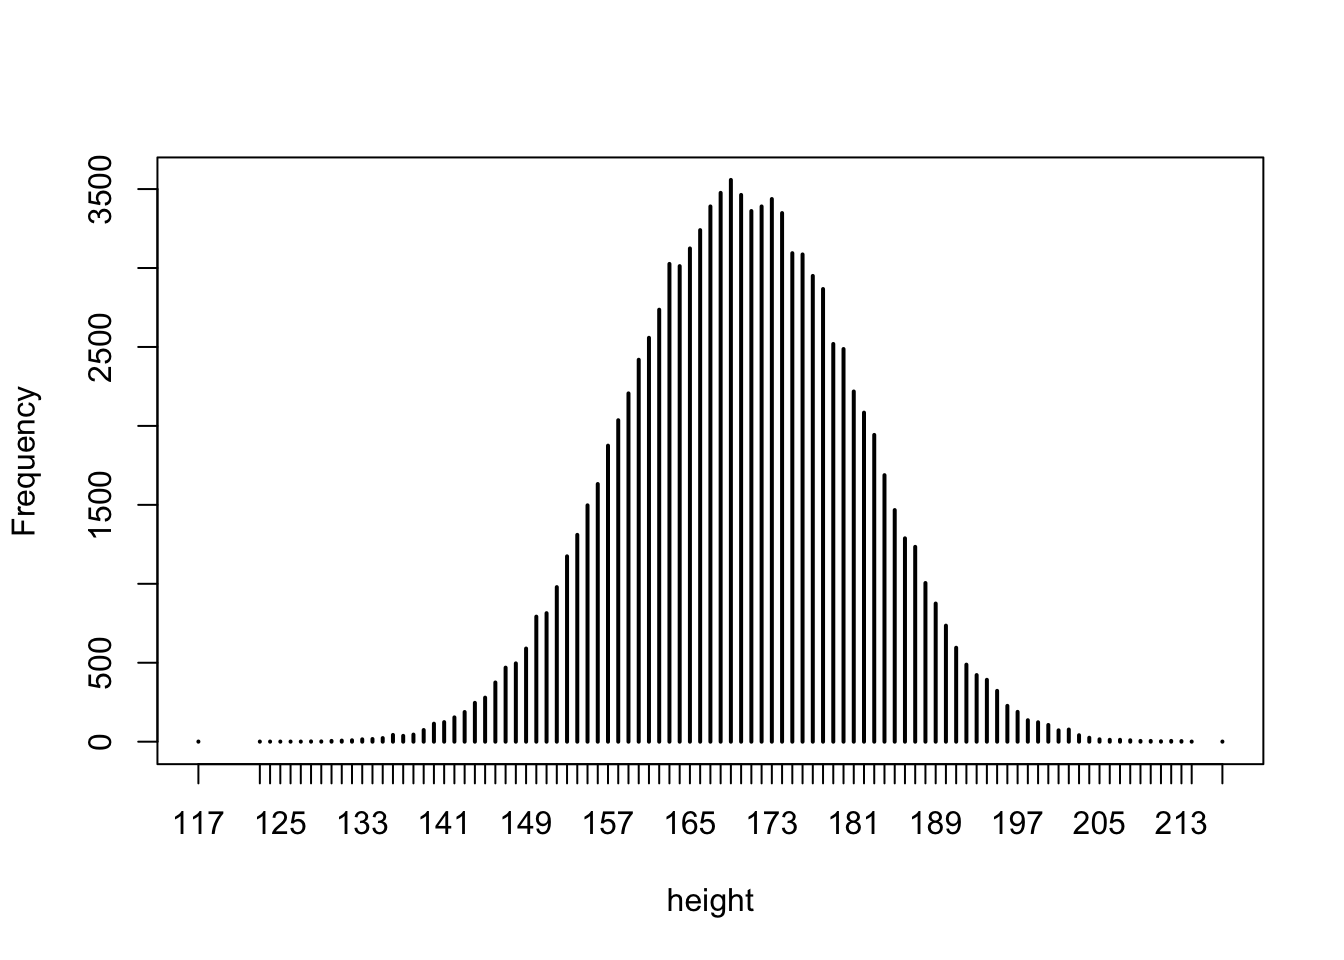
\includegraphics[width=0.6\linewidth]{statthink_files/figure-latex/Prob1-1} 

}

\caption{Bar Plot of Height}\label{fig:Prob1}
\end{figure}

Let us concentrate on the variable ``\texttt{height}''. A bar plot of the
distribution of the heights in the entire population is given in
Figure~\ref{fig:Prob1}~\footnote{Such a bar plot can be produced with the expression
  ``\texttt{plot(table(pop.1\$height))}''.}. Recall that a vertical bar is placed
above each value of height that appears in the population, with the
height of the bar representing the frequency of the value in the
population. One may read out of the graph or obtain from the numerical
summaries that the variable takes integer values in the range between
117 and 217 (heights are rounded to the nearest centimeter). The
distribution is centered at 170 centimeter, with the central 50\% of the
values spreading between 162 and 178 centimeters.

The mean of the height in the entire population is equal to 170
centimeter. This mean, just like the mean for the distribution of data,
is obtained by the summation of all the heights in the population
divided by the population size. Let us denote the size of the entire
population by \(N\). In this example \(N = 100,000\). (The size of the
sample for the data was called \(n\) and was equal to \(n=100\) in the
parallel example that deals with the data of a sample.) The mean of an
entire population is denoted by the Greek letter \(\mu\) and is read
``\emph{mew}''. (The average for the data was denoted \(\bar x\)). The formula of
the population mean is:

\[\mu = \frac{\mbox{Sum of all values in the population}}{\mbox{Number of values in the population}}= \frac{\sum_{i=1}^N x_i}{N}\;.\]

Observe the similarity between the definition of the mean for the data
and the definition of the mean for the population. In both cases the
arithmetic average is computed. The only difference is that in the case
of the mean of the data the computation is with respect to the values
that appear in the sample whereas for the population all the values in
the population participate in the computation.

In actual life, we will not have all the values of a variable in the
entire population. Hence, we will not be able to compute the actual
value of the population mean. However, it is still meaningful to talk
about the population mean because this number exists, even though we do
not know what its value is. As a matter of fact, one of the issues in
statistics is to try to estimate this unknown quantity on the basis of
the data we do have in the sample.

A characteristic of the distribution of an entire population is called a
\emph{parameter}. Hence, \(\mu\), the population average, is a parameter. Other
examples of parameters are the population median and the population
quartiles. These parameters are defined exactly like their data
counterparts, but with respect to the values of the entire population
instead of the observations in the sample alone.

Another example of a parameter is the population variance. Recall that
the sample variance was defined with the aid of the deviations
\(x_i - \bar x\), where \(x_i\) is the value of the measurement for the
\(i\)th subject and \(\bar x\) is the mean for the data. In order to compute
the sample variance these deviations were squared to produce the squared
deviations. The squares were summed up and then divided by the sample
size minus one (\(n-1\)). The sample variance, computed from the data, was
denoted \(s^2\).

The population variance is defined in a similar way. First, the
deviations from the population mean \(x_i - \mu\) are considered for each
of the members of the population. These deviations are squared and the
average of the squares is computed. We denote this parameter by
\(\sigma^2\) (read ``\emph{sigma square}''). A minor difference between the
sample variance and the population variance is that for the latter we
should divide the sum of squared deviations by the population size (\(N\))
and not by the population size minus one (\(N-1\)):

\[\begin{aligned}
\sigma^2 =& \mbox{The average square deviation in the population}\\
         =& \frac{\mbox{Sum of the squares of the deviations in the population}}{\mbox{Number of values in the population}}\\
         =& \frac{\sum_{i=1}^N (x_i-\mu)^2}{N}\;.\end{aligned}\]

The standard deviation of the population, yet another parameter, is
denoted by \(\sigma\) and is equal to the square root of the variance. The
standard deviation summarizes the overall variability of the measurement
across the population. Again, the typical situation is that we do not
know what the actual value of the standard deviation of the population
is. Yet, we may refer to it as a quantity and we may try to estimate its
value based on the data we do have from the sample.

For the height of the subjects in our imaginary city we get that the
variance is equal to \(\sigma^2 =126.1576\). The standard deviation is
equal to \(\sigma = \sqrt{126.1576} = 11.23199\). These quantities can be
computed in this example from the data frame ``\texttt{pop.1}'' with the aid of
the functions ``\texttt{var}'' and ``\texttt{sd}'', respectively\footnote{Observe that the function ``\texttt{var}'' computes the sample variance.
  Consequently, the sum of squares is divided by \(N-1\). We can correct
  that when computing the population variance by multiplying the
  result by \(N-1\) and dividing by \(N\). Notice that the difference
  between the two quantities is negligible for a large population.
  Henceforth we will use the functions ``\texttt{var}'' and ``\texttt{sd}'' to compute
  the variance and standard deviations of populations without the
  application of the correction.}.

\hypertarget{random-variables}{%
\section{Random Variables}\label{random-variables}}

In the previous section we dealt with the variability of the population.
Next we consider the variability of a random variable. As an example,
consider taking a sample of size \(n=1\) from the population (a single
person) and measuring his/her height.

The object \texttt{pop.1\$height} is a sequence with 100,000 entries. Think of
it as a population. We will apply the function ``\texttt{sample}'' to this
sequence:

\begin{Shaded}
\begin{Highlighting}[]
\KeywordTok{sample}\NormalTok{(pop}\FloatTok{.1}\OperatorTok{$}\NormalTok{height,}\DecValTok{1}\NormalTok{)}
\end{Highlighting}
\end{Shaded}

\begin{verbatim}
## [1] 175
\end{verbatim}

The first entry to the function is the given sequence of heights. When
we set the second argument to 1 then the function selects one of the
entries of the sequence at random, with each entry having the same
likelihood of being selected. Specifically, in this example an entry
that contains the value 162 was selected. Let us run the function again:

\begin{Shaded}
\begin{Highlighting}[]
\KeywordTok{sample}\NormalTok{(pop}\FloatTok{.1}\OperatorTok{$}\NormalTok{height,}\DecValTok{1}\NormalTok{)}
\end{Highlighting}
\end{Shaded}

\begin{verbatim}
## [1] 173
\end{verbatim}

In this instance an entry with a different value was selected. Try to
run the command several times yourself and see what you get. Would you
necessarily obtain a different value in each run?

Now let us enter the same command without pressing the return key:

\begin{Shaded}
\begin{Highlighting}[]
\KeywordTok{sample}\NormalTok{(pop}\FloatTok{.1}\OperatorTok{$}\NormalTok{height,}\DecValTok{1}\NormalTok{)}
\end{Highlighting}
\end{Shaded}

Can you tell, before pressing the key, what value will you get?

The answer to this question is of course \emph{``No''}. There are 100,000
entries with a total of 94 distinct values. In principle, any of the
values may be selected and there is no way of telling in advance which
of the values will turn out as an outcome.

A random variable is the future outcome of a measurement, {\textbf{before}}
the measurement is taken. It does not have a specific value, but rather
a collection of potential values with a distribution over these values.
After the measurement is taken and the specific value is revealed then
the random variable ceases to be a random variable! Instead, it becomes
data.

Although one is not able to say what the outcome of a random variable
will turn out to be. Still, one may identify patterns in this potential
outcome. For example, knowing that the distribution of heights in the
population ranges between 117 and 217 centimeter one may say in advance
that the outcome of the measurement must also be in that interval.
Moreover, since there is a total of 3,476 subjects with height equal to
168 centimeter and since the likelihood of each subject to be selected
is equal then the likelihood of selecting a subject of this height is
3,476/100,000 = 0.03476. In the context of random variables we call this
likelihood \emph{probability}. In the same vain, the frequency of subjects
with hight 192 centimeter is 488, and therefore the probability of
measuring such a height is 0.00488. The frequency of subjects with
height 200 centimeter or above is 393, hence the probability of
obtaining a measurement in the range between 200 and 217 centimeter is
0.00393.

\hypertarget{sample-space-and-distribution}{%
\subsection{Sample Space and Distribution}\label{sample-space-and-distribution}}

Let us turn to the formal definition of a random variable: A random
variable refer to numerical values, typically the outcome of an
observation, a measurement, or a function thereof.

A random variable is characterized via the collection of potential
values it may obtain, known as the \emph{sample space} and the likelihood of
obtaining each of the values in the sample space (namely, the
probability of the value). In the given example, the sample space
contains the 94 integer values that are marked in
Figure~\ref{fig:Prob1}. The probability of each value is the height
of the bar above the value, divided by the total frequency of 100,000
(namely, the relative frequency in the population).

We will denote random variables with capital Latin letters such as \(X\),
\(Y\), and \(Z\). Values they may obtain will be marked by small Latin
letters such as \(x\), \(y\), \(z\). For the probability of values we will use
the letter ``\(\Prob\)''. Hence, if we denote by \(X\) the measurement of
height of a random individual that is sampled from the given population
then:

\[\Prob(X = 168) = 0.03476\] and
\[\Prob(X \geq 200) = 0.00393\;.\]

Consider, as yet another example, the probability that the height of a
random person sampled from the population differs from 170 centimeter by
no more than 10 centimeters. (In other words, that the height is between
160 and 180 centimeters.) Denote by \(X\) the height of that random
person. We are interested in the probability
\(\Prob(|X -170| \leq 10)\).\footnote{The expression \(\{|X -170| \leq 10\}\) reads as ``the absolute value
  of the difference between \(X\) and 170 is no more that 10''. In other
  words, \(\{-10 \leq X - 170 \leq 10\}\), which is equivalent to the
  statement that \(\{160 \leq X \leq 180\}\). It follows that
  \(\Prob(|X-170|\leq 10) = \Prob(160\leq X \leq 180)\).}

The random person can be any of the subjects of the population with
equal probability. Thus, the sequence of the heights of the 100,000
subjects represents the distribution of the random variable \(X\):

\begin{Shaded}
\begin{Highlighting}[]
\NormalTok{pop}\FloatTok{.1}\NormalTok{ <-}\StringTok{ }\KeywordTok{read.csv}\NormalTok{(}\DataTypeTok{file=}\StringTok{"_data/pop1.csv"}\NormalTok{)}
\NormalTok{X <-}\StringTok{ }\NormalTok{pop}\FloatTok{.1}\OperatorTok{$}\NormalTok{height}
\end{Highlighting}
\end{Shaded}

Notice that the object ``\texttt{X}'' is a sequence of lenght 100,000 that stores
all the heights of the population. The probability we seek is the
relative frequency in this sequency of values between 160 and 180. First
we compute the probability and then explain the method of computation:

\begin{Shaded}
\begin{Highlighting}[]
\KeywordTok{mean}\NormalTok{(}\KeywordTok{abs}\NormalTok{(X}\DecValTok{-170}\NormalTok{) }\OperatorTok{<=}\StringTok{ }\DecValTok{10}\NormalTok{)}
\end{Highlighting}
\end{Shaded}

\begin{verbatim}
## [1] 0.64541
\end{verbatim}

We get that the height of a person randomly sampled from the population
is between 160 and 180 centimeters with probability 0.64541.

Let us produce a small example that will help us explain the computation
of the probability. We start by forming a sequence with 10 numbers:

\begin{Shaded}
\begin{Highlighting}[]
\NormalTok{Y <-}\StringTok{ }\KeywordTok{c}\NormalTok{(}\FloatTok{6.3}\NormalTok{, }\FloatTok{6.9}\NormalTok{, }\FloatTok{6.6}\NormalTok{, }\FloatTok{3.4}\NormalTok{, }\FloatTok{5.5}\NormalTok{, }\FloatTok{4.3}\NormalTok{, }\FloatTok{6.5}\NormalTok{, }\FloatTok{4.7}\NormalTok{, }\FloatTok{6.1}\NormalTok{, }\FloatTok{5.3}\NormalTok{)}
\end{Highlighting}
\end{Shaded}

The goal is to compute the proportion of numbers that are in the range
\([4,6]\) (or, equivalently, \(\{|Y-5| \leq 1\}\)).

The function ``\texttt{abs}'' computes the absolute number of its input argument.
When the function is applied to the sequence ``\texttt{Y-5}'' it produces a
sequence of the same length with the distances between the components of
``\texttt{Y}'' and the number 5:

\begin{Shaded}
\begin{Highlighting}[]
\KeywordTok{abs}\NormalTok{(Y}\DecValTok{-5}\NormalTok{)}
\end{Highlighting}
\end{Shaded}

\begin{verbatim}
##  [1] 1.3 1.9 1.6 1.6 0.5 0.7 1.5 0.3 1.1 0.3
\end{verbatim}

Compare the resulting output to the original sequence. The first value
in the input sequence is 6.3. Its distance from 5 is indeed 1.3. The
fourth value in the input sequence is 3.4. The difference 3.4 - 5 is
equal to -1.6, and when the absolute value is taken we get a distance of
1.6.

The function ``\texttt{\textless{}=}'' expects an argument to the right and an argument to
the left. It compares each component to the left with the parallel
component to the right and returns a logical value, ``\texttt{TRUE}'' or
``\texttt{FALSE}'', depending on whether the relation that is tested holds or
not:

\begin{Shaded}
\begin{Highlighting}[]
\KeywordTok{abs}\NormalTok{(Y }\OperatorTok{-}\StringTok{ }\DecValTok{5}\NormalTok{) }\OperatorTok{<=}\StringTok{ }\DecValTok{1}
\end{Highlighting}
\end{Shaded}

\begin{verbatim}
##  [1] FALSE FALSE FALSE FALSE  TRUE  TRUE FALSE  TRUE FALSE  TRUE
\end{verbatim}

Observe the in this example the function ``\texttt{\textless{}=}'' produced 10 logical
values, one for each of the elements of the sequence to the left of it.
The first input in the sequence ``\texttt{Y}'' is 6.3, which is more than one
unit away from 5. Hence, the first output of the logical expression is
``\texttt{FALSE}''. On the other hand, the last input in the sequence ``\texttt{Y}'' is
5.3, which is within the range. Therefore, the last output of the
logical expression is ``\texttt{TRUE}''.

Next, we compute the proportion of ``\texttt{TRUE}'' values in the sequence:

\begin{Shaded}
\begin{Highlighting}[]
\KeywordTok{mean}\NormalTok{(}\KeywordTok{abs}\NormalTok{(Y }\OperatorTok{-}\StringTok{ }\DecValTok{5}\NormalTok{) }\OperatorTok{<=}\StringTok{ }\DecValTok{1}\NormalTok{)}
\end{Highlighting}
\end{Shaded}

\begin{verbatim}
## [1] 0.4
\end{verbatim}

When a sequence with logical values is entered into the function
``\texttt{mean}'' then the function replaces the \texttt{TRUE}'s by 1 and the \texttt{FALSE}'s
by 0. The average produces then the relative frequency of \texttt{TRUE}'s in
the sequence as required. Specifically, in this example there are 4
\texttt{TRUE}'s and 6 \texttt{FALSE}'s. Consequently, the output of the final
expression is \(4/10 = 0.4\).

The computation of the probability that the sampled height falls within
10 centimeter of 170 is based on the same code. The only differences are
that the input sequence ``\texttt{Y}'' is replaced by the sequence of population
heights ``\texttt{X}'' as input. the number ``\texttt{5}'' is replaced by the number
``\texttt{170}'' and the number ``\texttt{1}'' is replaced by the number ``\texttt{10}''. In both
cases the result of the computation is the relative proportion of the
times that the values of the input sequence fall within a given range of
the indicated number.

The probability function of a random variable is defined for any value
that the random variable may obtain and produces the \emph{distribution} of
the random variable. The probability function may emerge as a relative
frequency as in the given example or it may be a result of theoretical
modeling. Examples of theoretical random variables are presented mainly
in the next two chapters.

Consider an example of a random variable. The sample space and the
probability function specify the distribution of the random variable.
For example, assume it is known that a random variable \(X\) may obtain
the values 0, 1, 2, or 3. Moreover, imagine that it is known that
\(\Prob(X=1) = 0.25\), \(\Prob(X=2) = 0.15\), and \(\Prob(X=3)= 0.10\). What
is \(\Prob(X=0)\), the probability that \(X\) is equal to 0?

The sample space, the collection of possible values that the random
variable may obtain is the collection \(\{0,1,2,3\}\). Observe that the
sum over the positive values is:

\[\Prob(X > 0) = \Prob(X=1) + \Prob(X=2) + \Prob(X=3) = 0.25 + 0.15 + 0.10 = 0.50\;.\]
It follows, since the sum of probabilities over the entire sample space
is equal to 1, that \(\Prob(X=0) = 1- 0.5 = 0.5\).

\begin{table}[t]

\caption{\label{tab:Probability1}The Distribution of $X$}
\centering
\begin{tabular}{rrr}
\toprule
Value & Probability & Cum.Prob\\
\midrule
0 & 0.50 & 0.50\\
1 & 0.25 & 0.75\\
2 & 0.15 & 0.90\\
3 & 0.10 & 1.00\\
\bottomrule
\end{tabular}
\end{table}

Table~\ref{tab:Probability1} summarizes the distribution of the random
variable \(X\). Observe the similarity between the probability function
and the notion of relative frequency that was discussed in
Chapter~\ref{ChapData}. Both quantities describe distribution. Both are
non-negative and sum to 1. Likewise, notice that one may define the
cumulative probability the same way cumulative relative frequency is
defined: Ordering the values of the random variable from smallest to
largest, the cumulative probability at a given value is the sum of
probabilities for values less or equal to the given value.

Knowledge of the probabilities of a random variable (or the cumulative
probabilities) enables the computation of other probabilities that are
associated with the random variable. For example, considering the random
variable \(X\) of Table~\ref{tab:Probability1}, we may calculate the
probability of \(X\) falling in the interval \([0.5, 2.3]\). Observe that
the given range contains two values from the sample space, 1 and 2,
therefore:

\[\Prob(0.5 \leq X \leq 2.3) = \Prob(X=1) + \Prob(X = 2) = 0.25 + 0.15 = 0.40\;.\]
Likewise, we may produce the probability of \(X\) obtaining an odd value:

\[\Prob(X = \mbox{odd}) = \Prob(X=1) + \Prob(X=3) = 0.25 + 0.10 = 0.35\;.\]
Observe that both \(\{0.5 \leq X \leq 2.3\}\) and \(\{X = \mbox{odd}\}\)
refer to subsets of values of the sample space. Such subsets are denoted
\emph{events}. In both examples the probability of the event was computed by
the summation of the probabilities associated with values that belong to
the event.

\hypertarget{expectation-and-standard-deviation}{%
\subsection{Expectation and Standard Deviation}\label{expectation-and-standard-deviation}}

We may characterize the center of the distribution of a random variable
and the spread of the distribution in ways similar to those used for the
characterization of the distribution of data and the distribution of a
population.

The \emph{expectation} marks the center of the distribution of a random
variable. It is equivalent to the data average \(\bar x\) and the
population average \(\mu\), which was used in order to mark the location
of the distribution of the data and the population, respectively.

Recall from Chapter~\ref{ChapDescriptiveStat} that the average of the data
can be computed as the weighted average of the values that are present
in the data, with weights given by the relative frequency. Specifically,
we saw for the data

\[1,\; 1,\; 1,\; 2,\; 2,\; 3,\; 4,\; 4,\; 4,\; 4,\; 4\] that

\[\frac{1 + 1 + 1 + 2 + 2 + 3 + 4 + 4 + 4 + 4 + 4}{11} =
1\times \frac{3}{11} + 2 \times \frac{2}{11} + 3 \times \frac{1}{11} + 4 \times \frac{5}{11}\;,\]
producing the value of \(\bar x =2.727\) in both representations. Using a
formula, the equality between the two ways of computing the mean is
given in terms of the equation:

\[\bar x = \frac{\sum_{i=1}^n x_i}{n} = \sum_x \big(x \times (f_x/n)\big)\;.\]
In the first representation of the arithmetic mean, the average is
computed by the summation of all data points and dividing the sum by the
sample size. In the second representation, that uses a weighted sum, the
sum extends over all the unique values that appear in the data. For each
unique value the value is multiplied by the relative frequency of the
value in the data. These multiplications are summed up to produce the
mean.

The expectation of a random variable is computed in the spirit of the
second formulation. The expectation of a random variable is marked with
the letter ``\(\Expec\)'' and is define via the equation:

\[\Expec(X) = \sum_x \big(x \times \Prob(x)\big)\;.\] In this definition
all the unique values of the sample space are considered. For each value
a product of the value and the probability of the value is taken. The
expectation is obtained by the summation of all these products. In this
definition the probability \(\Prob(x)\) replaces the relative frequency
\(f_x/n\) but otherwise, the definition of the expectation and the second
formulation of the mean are identical to each other.

Consider the random variable \(X\) with distribution that is described in
Table~\ref{tab:Probability1}. In order to obtain its expectation we
multiply each value in the sample space by the probability of the value.
Summation of the products produces the expectation (see
Table~\ref{tab:Probability1}:

\[\Expec(X) = 0 \times 0.5 + 1 \times 0.25 + 2 \times 0.15 + 3\times 0.10 = 0.85\;.\]

\begin{table}[t]

\caption{\label{tab:Probability2}The Expectation of $X$}
\centering
\begin{tabular}{rrr}
\toprule
Value & Probability & Value * Probability\\
\midrule
0 & 0.50 & 0.00\\
1 & 0.25 & 0.25\\
2 & 0.15 & 0.30\\
3 & 0.10 & 0.30\\
\bottomrule
\end{tabular}
\end{table}

\begin{verbatim}
## Expectation = sum(Value*Probability) =  0.85
\end{verbatim}

In the example of height we get that the expectation is equal to 170.035
centimeter. Notice that this expectation is equal to \(\mu\), the mean of
the population\footnote{The mean of the population can be computed with the expression
  ``\texttt{mean(pop.1\$height)}''}. This is no accident. The expectation of a potential
measurement of a randomly selected subject from a population is equal to
the average of the measurement across all subjects.

The sample variance (\(s^2\)) is obtained as the sum of the squared
deviations from the average, divided by the sample size (\(n\)) minus 1:

\[s^2 = \frac{\sum_{i=1}^n (x_i - \bar x)^2}{n-1}\;.\] A second
formulation for the computation of the same quantity is via the use of
relative frequencies. The formula for the sample variance takes the form

\[s^2 = \frac{n}{n-1}\sum_x \big((x - \bar x)^2\times (f_x/n)\big)\;.\]
In this formulation one considers each of the unique value that are
present in the data. For each value the deviation between the value and
the average is computed. These deviations are then squared and
multiplied by the relative frequency. The products are summed up.
Finally, the sum is multiplied by the ratio between the sample size \(n\)
and \(n-1\) in order to correct for the fact that in the sample variance
the sum of squared deviations is divided by the sample size minus 1 and
not by the sample size.

In a similar way, the variance of a random variable may be defined via
the probability of the values that make the sample space. For each such
value one computes the deviation from the expectation. This deviation is
then squared and multiplied by the probability of the value. The
multiplications are summed up in order to produce the variance:

\[\Var(X) = \sum_x\big( (x-\Expec(X))^2 \times \Prob(x)\big)\;.\] Notice
that the formula for the computation of the variance of a random
variable is very similar to the second formulation for the computation
of the sample variance. Essentially, the mean of the data is replaced by
the expectation of the random variable and the relative frequency of a
value is replaced by the probability of the value. Another difference is
that the correction factor is not used for the variance of a random
variable.

\begin{table}[t]

\caption{\label{tab:tab3}The Variance of $X$}
\centering
\begin{tabular}{rrrrr}
\toprule
\$x\$ & \$P(X=x)\$ & \$x - E[X]\$ & \$(x - E[X])\textasciicircum{}2\$ & \$P(X=x)*(x - E[X])\textasciicircum{}2\$\\
\midrule
0 & 0.50 & -0.85 & 0.7225 & 0.361250\\
1 & 0.25 & 0.15 & 0.0225 & 0.005625\\
2 & 0.15 & 1.15 & 1.3225 & 0.198375\\
3 & 0.10 & 2.15 & 4.6225 & 0.462250\\
\bottomrule
\end{tabular}
\end{table}

\begin{verbatim}
## Var = sum(p*(x-sum(p*x))^2) =  1.0275
\end{verbatim}

As an example consider the variance of the random variable \(X\). The
computation of the variance of this random variable is carried out in
Table~\ref{tab:tab3}. The sample space, the values that the
random variable may obtain, are given in the first column and the
probabilities of the values are given in the second column. In the third
column the deviation of the value from the expectation
\(\Expec(X) = 0.85\) is computed for each value. The 4th column contains
the square of these deviations and the 5th and last column involves the
product of the square deviations and the probabilities. The variance is
obtained by summing up the products in the last column. In the given
example:

\[\begin{aligned}
\Var(X) = & (0-0.85)^2 \times 0.5  + (1-0.85)^2 \times 0.25 \\ &+ (2-0.85)^2\times 0.15 + (3-0.85)^2\times 0.10= 1.0275\;.\end{aligned}\]

The standard deviation of a random variable is the square root of the
variance. The standard deviation of \(X\) is
\(\sqrt{\Var(X)} = \sqrt{1.0275} = 1.013657\).

In the example that involves the height of a subject selected from the
population at random we obtain that the variance is \(126.1576\), equal to
the population variance, and the standard deviation is 11.23199, the
square root of the variance.

Other characterization of the distribution that were computed for data,
such as the median, the quartiles, etc., may also be defined for random
variables.

\hypertarget{probability-and-statistics}{%
\section{Probability and Statistics}\label{probability-and-statistics}}

Modern science may be characterized by a systematic collection of
empirical measurements and the attempt to model laws of nature using
mathematical language. The drive to deliver better measurements led to
the development of more accurate and more sensitive measurement tools.
Nonetheless, at some point it became apparent that measurements may not
be perfectly reproducible and any repeated measurement of presumably the
exact same phenomena will typically produce variability in the outcomes.
On the other hand, scientists also found that there are general laws
that govern this variability in repetitions. For example, it was
discovered that the average of several independent repeats of the
measurement is less variable and more reproducible than each of the
single measurements themselves.

Probability was first introduced as a branch of mathematics in the
investigation of uncertainty associated with gambling and games of
chance. During the early 19th century probability began to be used in
order to model variability in measurements. This application of
probability turned out to be very successful. Indeed, one of the major
achievements of probability was the development of the mathematical
theory that explains the phenomena of reduced variability that is
observed when averages are used instead of single measurements. In
Chapter~\ref{ChapSampDist} we discuss the conclusions of this theory.

Statistics study method for inference based on data. Probability serves
as the mathematical foundation for the development of statistical
theory. In this chapter we introduced the probabilistic concept of a
random variable. This concept is key for understanding statistics. In
the rest of Part I of this book we discuss the probability theory that
is used for statistical inference. Statistical inference itself is
discussed in Part II of the book.

\hypertarget{exercises-3}{%
\section{Exercises}\label{exercises-3}}

\begin{table}[t]

\caption{\label{tab:tab4}The Distribution of $Y$}
\centering
\begin{tabular}{rl}
\toprule
Value & Probability\\
\midrule
0 & 1p\\
1 & 2p\\
2 & 3p\\
3 & 4p\\
4 & 5p\\
\addlinespace
5 & 6p\\
\bottomrule
\end{tabular}
\end{table}

\BeginKnitrBlock{exercise}
\protect\hypertarget{exr:unnamed-chunk-50}{}{\label{exr:unnamed-chunk-50} }Table~\ref{tab:tab4} presents the
probabilities of the random variable \(Y\).

These probabilities are a
function of the number \(p\), the probability of the value ``0''. Answer the
following questions:

\begin{enumerate}
\def\labelenumi{\arabic{enumi}.}
\item
  What is the value of \(p\)?
\item
  \(\Prob(Y <3 )\) = ?
\item
  \(\Prob(Y = \mbox{odd})\) = ?
\item
  \(\Prob(1 \leq Y < 4)\) = ?
\item
  \(\Prob(|Y -3| < 1.5)\) = ?
\item
  \(\Expec(Y)\) = ?
\item
  \(\Var(Y)\) = ?
\item
  What is the standard deviation of \(Y\).
\end{enumerate}
\EndKnitrBlock{exercise}

\BeginKnitrBlock{exercise}
\protect\hypertarget{exr:unnamed-chunk-51}{}{\label{exr:unnamed-chunk-51} }One invests \$2 to participate in a game of chance.
In this game a coin is tossed three times. If all tosses end up ``Head''
then the player wins \$10. Otherwise, the player losses the investment.

\begin{enumerate}
\def\labelenumi{\arabic{enumi}.}
\item
  What is the probability of winning the game?
\item
  What is the probability of loosing the game?
\item
  What is the expected gain for the player that plays this game?
  (Notice that the expectation can obtain a negative value.)
\end{enumerate}
\EndKnitrBlock{exercise}

\hypertarget{summary-3}{%
\section{Summary}\label{summary-3}}

\hypertarget{glossary}{%
\subsection*{Glossary}\label{glossary}}


\begin{description}
\item[Random Variable:]
The probabilistic model for the value of a measurement, before the
measurement is taken.
\item[Sample Space:]
The set of all values a random variable may obtain.
\item[Probability:]
A number between 0 and 1 which is assigned to a subset of the sample
space. This number indicates the likelihood of the random variable
obtaining a value in that subset.
\item[Expectation:]
The central value for a random variable. The expectation of the
random variable \(X\) is marked by \(\Expec(X)\).
\item[Variance:]
The (squared) spread of a random variable. The variance of the
random variable \(X\) is marked by \(\Var(X)\). The standard deviation
is the square root of the variance.
\end{description}

\hypertarget{discussion-in-the-forum}{%
\subsection*{Discussion in the Forum}\label{discussion-in-the-forum}}


Random variables are used to model situations in which the outcome,
before the fact, is uncertain. One component in the model is the sample
space. The sample space is the list of all possible outcomes. It
includes the outcome that took place, but also all other outcomes that
could have taken place but never did materialize. The rationale behind
the consideration of the sample space is the intention to put the
outcome that took place in context. What do you think of this rationale?

When forming your answer to this question you may give an example of a
situation from you own field of interest for which a random variable can
serve as a model. Identify the sample space for that random variable and
discuss the importance (or lack thereof) of the correct identification
of the sample space.

For example, consider a factory that produces car parts that are sold to
car makers. The role of the QA personnel in the factory is to validate
the quality of each batch of parts before the shipment to the client.

To achieve that, a sample of parts may be subject to a battery of
quality test. Say that 20 parts are selected to the sample. The number
of those among them that will not pass the quality testing may be
modeled as a random variable. The sample space for this random variable
may be any of the numbers 0, 1, 2, \ldots{}, 20.

The number 0 corresponds to the situation where all parts in the sample
passed the quality testing. The number 1 corresponds to the case where 1
part did not pass and the other 19 did. The number 2 describes the case
where 2 of the 20 did not pass and 18 did pass, etc.

\hypertarget{summary-of-formulas}{%
\subsection*{Summary of Formulas}\label{summary-of-formulas}}


\begin{description}
\item[Population Size:]
\(N\) = the number of people, things, etc. in the population.
\item[Population Average:]
\(\mu = (1/N)\sum_{i=1}^N x_i\)
\item[Expectation of a Random Variable:]
\(\Expec(X) = \sum_x \big(x \times \Prob(x)\big)\)
\item[Population Variance:]
\(\sigma^2 = (1/N)\sum_{i=1}^N (x_i-\mu)^2\)
\item[Variance of a Random Variable:]
\(\Var(X) = \sum_x\big( (x-\Expec(X))^2 \times \Prob(x)\big)\)
\end{description}

\hypertarget{ChapRandomVar}{%
\chapter{Random Variables}\label{ChapRandomVar}}

\hypertarget{student-learning-objective-1}{%
\section{Student Learning Objective}\label{student-learning-objective-1}}

This section introduces some important examples of random variables. The
distributions of these random variables emerge as mathematical models of
real-life settings. In two of the examples the sample space is composed
of integers. In the other two examples the sample space is made of
continuum of values. For random variables of the latter type one may use
the density, which is a type of a histogram, in order to describe the
distribution.

By the end of the chapter the student should:

\begin{itemize}
\item
  Identify the Binomial, Poisson, Uniform, and Exponential random
  variables, relate them to real life situations, and memorize their
  expectations and variances.
\item
  Relate the plot of the density/probability function and the
  cumulative probability function to the distribution of a random
  variable.
\item
  Become familiar with the \texttt{R} functions that produce the
  density/probability of these random variables and their cumulative
  probabilities.
\item
  Plot the density and the cumulative probability function of a random
  variable and compute probabilities associated with random variables.
\end{itemize}

\hypertarget{discrete-random-variables}{%
\section{Discrete Random Variables}\label{discrete-random-variables}}

In the previous chapter we introduced the notion of a random variable. A
random variable corresponds to the outcome of an observation or a
measurement prior to the actual making of the measurement. In this
context one can talk of all the values that the measurement may
potentially obtain. This collection of values is called the \emph{sample
space}. To each value in the sample space one may associate the
\emph{probability} of obtaining this particular value. Probabilities are like
relative frequencies. All probabilities are positive and the sum of the
probabilities that are associated with all the values in the sample
space is equal to one.

A random variable is defined by the identification of its sample space
and the probabilities that are associated with the values in the sample
space. For each type of random variable we will identify first the
sample space --- the values it may obtain --- and then describe the
probabilities of the values. Examples of situations in which each type
of random variable may serve as a model of a measurement will be
provided. The \texttt{R} system provides functions for the computation of
probabilities associated with specific types of random variables. We
will use these functions in this and in proceeding chapters in order to
carry out computations associated with the random variables and in order
to plot their distributions.

The distribution of a random variable, just like the distribution of
data, can be characterized using numerical summaries. For the latter we
used summaries such as the mean and the sample variance and standard
deviation. The mean is used to describe the central location of the
distribution and the variance and standard deviation are used to
characterize the total spread. Parallel summaries are used for random
variable. In the case of a random variable the name \emph{expectation} is
used for the central location of the distribution and the \emph{variance} and
the \emph{standard deviation} (the square root of the variation) are used to
summarize the spread. In all the examples of random variables we will
identify the expectation and the variance (and, thereby, also the
standard deviation).

Random variables are used as probabilistic models of measurements.
Theoretical considerations are used in many cases in order to define
random variables and their distribution. A random variable for which the
values in the sample space are separated from each other, say the values
are integers, is called a \emph{discrete random variable}. In this section we
introduce two important integer-valued random variables: The \emph{Binomial}
and the \emph{Poisson} random variables. These random variables may emerge as
models in contexts where the measurement involves counting the number of
occurrences of some phenomena.

Many other models, apart from the Binomial and Poisson, exist for
discrete random variables. An example of such model, the
Negative-Binomial model, will be considered in
Section~\ref{sec:RVarExercises}. Depending on the specific context that
involves measurements with discrete values, one may select the Binomial,
the Poisson, or one of these other models to serve as a theoretical
approximation of the distribution of the measurement.

\hypertarget{the-binomial-random-variable}{%
\subsection{The Binomial Random Variable}\label{the-binomial-random-variable}}

The Binomial random variable is used in settings in which a trial that
has two possible outcomes is repeated several times. Let us designate
one of the outcomes as ``Success'' and the other as ``Failure''. Assume that
the probability of success in each trial is given by some number \(p\)
that is larger than 0 and smaller than 1. Given a number \(n\) of repeats
of the trial and given the probability of success, the actual number of
trials that will produce ``Success'' as their outcome is a random
variable. We call such random variable \emph{Binomial}. The fact that a
random variable \(X\) has such a distribution is marked by the expression:
``\(X \sim \mathrm{Binomial}(n,p)\)''.

As an example consider tossing 10 coins. Designate ``Head'' as success and
``Tail'' as failure. For fair coins the probability of ``Head'' is \(1/2\).
Consequently, if \(X\) is the total number of ``Heads'' then
\(X \sim \mathrm{Binomial}(10,0.5)\), where \(n=10\) is the number of trials
and \(p=0.5\) is the probability of success in each trial.

It may happen that all 10 coins turn up ``Tail''. In this case \(X\) is
equal to 0. It may also be the case that one of the coins turns up
``Head'' and the others turn up ``Tail''. The random variable \(X\) will
obtain the value 1 in such a case. Likewise, for any integer between 0
and 10 it may be the case that the number of ``Heads'' that turn up is
equal to that integer with the other coins turning up ``Tail''. Hence, the
sample space of \(X\) is the set of integers \(\{0, 1, 2, \ldots, 10\}\).
The probability of each outcome may be computed by an appropriate
mathematical formula that will not be discussed here\footnote{If \(X\sim \mathrm{Binomial}(n,p)\) then
  \(\Prob(X = x) = {n \choose x} p^x (1-p)^{n-x}\), for
  \(x = 0, 1, \ldots, n\).}.

The probabilities of the various possible values of a Binomial random
variable may be computed with the aid of the \texttt{R} function ``\texttt{dbinom}''
(that uses the mathematical formula for the computation). The input to
this function is a sequence of values, the value of \(n\), and the value
of \(p\). The output is the sequence of probabilities associated with each
of the values in the first input.

\begin{figure}

{\centering 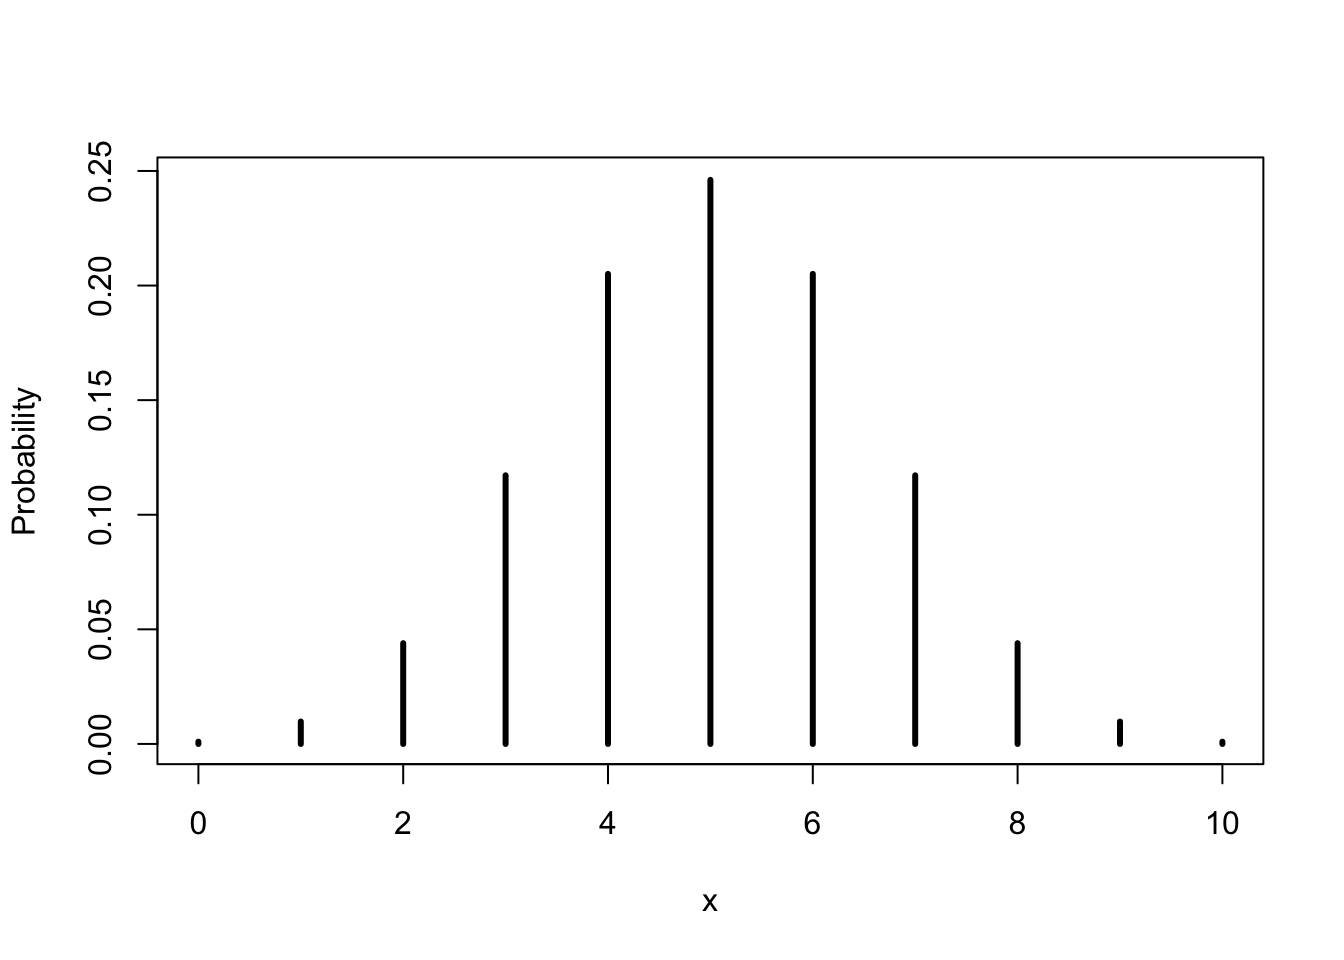
\includegraphics[width=0.6\linewidth]{statthink_files/figure-latex/RVar2-1} 

}

\caption{The Binomial(10,0.5) Distribution}\label{fig:RVar2}
\end{figure}

For example, let us use the function in order to compute the probability
that the given Binomial obtains an odd value. A sequence that contains
the odd values in the Binomial sample space can be created with the
expression ``\texttt{c(1,3,5,7,9)}''. This sequence can serve as the input in the
first argument of the function ``\texttt{dbinom}''. The other arguments are
``\texttt{10}'' and ``\texttt{0.5}'', respectively:

\begin{Shaded}
\begin{Highlighting}[]
\KeywordTok{dbinom}\NormalTok{(}\KeywordTok{c}\NormalTok{(}\DecValTok{1}\NormalTok{,}\DecValTok{3}\NormalTok{,}\DecValTok{5}\NormalTok{,}\DecValTok{7}\NormalTok{,}\DecValTok{9}\NormalTok{),}\DecValTok{10}\NormalTok{,}\FloatTok{0.5}\NormalTok{)}
\end{Highlighting}
\end{Shaded}

\begin{verbatim}
## [1] 0.009765625 0.117187500 0.246093750 0.117187500 0.009765625
\end{verbatim}

Observe that the output of the function is a sequence of the same length
as the first argument. This output contains the Binomial probabilities
of the values in the first argument. In order to obtain the probability
of the event \(\{\mbox{X is odd}\}\) we should sum up these probabilities,
which we can do by applying the function ``\texttt{sum}'' to the output of the
function that computes the Binomial probabilities:

\begin{Shaded}
\begin{Highlighting}[]
\KeywordTok{sum}\NormalTok{(}\KeywordTok{dbinom}\NormalTok{(}\KeywordTok{c}\NormalTok{(}\DecValTok{1}\NormalTok{,}\DecValTok{3}\NormalTok{,}\DecValTok{5}\NormalTok{,}\DecValTok{7}\NormalTok{,}\DecValTok{9}\NormalTok{),}\DecValTok{10}\NormalTok{,}\FloatTok{0.5}\NormalTok{))}
\end{Highlighting}
\end{Shaded}

\begin{verbatim}
## [1] 0.5
\end{verbatim}

Observe that the probability of obtaining an odd value in this specific
case is equal to one half.

Another example is to compute all the probabilities of all the potential
values of a \(\mathrm{Binomial}(10,0.5)\) random variable:

\begin{Shaded}
\begin{Highlighting}[]
\NormalTok{x <-}\StringTok{ }\DecValTok{0}\OperatorTok{:}\DecValTok{10}
\KeywordTok{dbinom}\NormalTok{(x,}\DecValTok{10}\NormalTok{,}\FloatTok{0.5}\NormalTok{)}
\end{Highlighting}
\end{Shaded}

\begin{verbatim}
##  [1] 0.0009765625 0.0097656250 0.0439453125 0.1171875000 0.2050781250
##  [6] 0.2460937500 0.2050781250 0.1171875000 0.0439453125 0.0097656250
## [11] 0.0009765625
\end{verbatim}

The expression ``\texttt{start.value:end.value}'' produces a sequence of numbers
that initiate with the number ``\texttt{start.value}'' and proceeds in jumps of
size one until reaching the number ``\texttt{end.value}''. In this example,
``\texttt{0:10}'' produces the sequence of integers between 0 and 10, which is
the sample space of the current Binomial example. Entering this sequence
as the first argument to the function ``\texttt{dbinom}'' produces the
probabilities of all the values in the sample space.

One may display the distribution of a discrete random variable with a
bar plot similar to the one used to describe the distribution of data.
In this plot a vertical bar representing the probability is placed above
each value of the sample space. The hight of the bar is equal to the
probability. A bar plot of the \(\mathrm{Binomial}(10,0.5)\) distribution
is provided in Figure~\ref{fig:RVar2}.

Another useful function is ``\texttt{pbinom}'', which produces the cumulative
probability of the Binomial:

\begin{Shaded}
\begin{Highlighting}[]
\KeywordTok{pbinom}\NormalTok{(x,}\DecValTok{10}\NormalTok{,}\FloatTok{0.5}\NormalTok{)}
\end{Highlighting}
\end{Shaded}

\begin{verbatim}
##  [1] 0.0009765625 0.0107421875 0.0546875000 0.1718750000 0.3769531250
##  [6] 0.6230468750 0.8281250000 0.9453125000 0.9892578125 0.9990234375
## [11] 1.0000000000
\end{verbatim}

\begin{Shaded}
\begin{Highlighting}[]
\KeywordTok{cumsum}\NormalTok{(}\KeywordTok{dbinom}\NormalTok{(x,}\DecValTok{10}\NormalTok{,}\FloatTok{0.5}\NormalTok{))}
\end{Highlighting}
\end{Shaded}

\begin{verbatim}
##  [1] 0.0009765625 0.0107421875 0.0546875000 0.1718750000 0.3769531250
##  [6] 0.6230468750 0.8281250000 0.9453125000 0.9892578125 0.9990234375
## [11] 1.0000000000
\end{verbatim}

The output of the function ``\texttt{pbinom}'' is the cumulative probability
\(\Prob(X \leq x)\) that the random variable is less than or equal to the
input value. Observe that this cumulative probability is obtained by
summing all the probabilities associated with values that are less than
or equal to the input value. Specifically, the cumulative probability at
\(x=3\) is obtained by the summation of the probabilities at \(x=0\), \(x=1\),
\(x=2\), and \(x=3\):

\[\Prob(X \leq 3) = 0.0009765625 + 0.009765625 + 0.0439453125 + 0.1171875 = 0.171875\]
The numbers in the sum are the first 4 values from the output of the
function ``\texttt{dbinom(x,10,0.5)}'', which computes the probabilities of the
values of the sample space.

In principle, the expectation of the Binomial random variable, like the
expectation of any other (discrete) random variable is obtained from the
application of the general formulae:

\[\Expec(X) = \sum_x \big(x \times \Prob(X = x)\big)\;,\quad \Var(X) = \sum_x\big( (x-\Expec(X))^2 \times \Prob(x)\big)\;.\]
However, in the specific case of the Binomial random variable, in which
the probability \(\Prob(X = x)\) obeys the specific mathematical formula
of the Binomial distribution, the expectation and the variance reduce to
the specific formulae:

\[\Expec(X) = n p\;,\quad \Var(X) = n p(1-p)\;.\]
Hence, the expectation is the product of the number of trials \(n\) with
the probability of success in each trial \(p\). In the variance the number
of trials is multiplied by the product of a probability of success (\(p\))
with the probability of a failure (\(1-p\)).

As illustration, let us compute for the given example the expectation
and the variance according to the general formulae for the computation
of the expectation and variance in random variables and compare the
outcome to the specific formulae for the expectation and variance in the
Binomial distribution:

\begin{Shaded}
\begin{Highlighting}[]
\NormalTok{X.val <-}\StringTok{ }\DecValTok{0}\OperatorTok{:}\DecValTok{10}
\NormalTok{P.val <-}\StringTok{ }\KeywordTok{dbinom}\NormalTok{(X.val,}\DecValTok{10}\NormalTok{,}\FloatTok{0.5}\NormalTok{)}
\NormalTok{EX <-}\StringTok{ }\KeywordTok{sum}\NormalTok{(X.val}\OperatorTok{*}\NormalTok{P.val)}
\NormalTok{EX}
\end{Highlighting}
\end{Shaded}

\begin{verbatim}
## [1] 5
\end{verbatim}

\begin{Shaded}
\begin{Highlighting}[]
\KeywordTok{sum}\NormalTok{((X.val}\OperatorTok{-}\NormalTok{EX)}\OperatorTok{^}\DecValTok{2}\OperatorTok{*}\NormalTok{P.val)}
\end{Highlighting}
\end{Shaded}

\begin{verbatim}
## [1] 2.5
\end{verbatim}

This agrees with the specific formulae for Binomial variables, since
\(10 \times 0.5 = 5\) and \(10 \times 0.5 \times(1-0.5) = 2.5\).

Recall that the general formula for the computation of the expectation
calls for the multiplication of each value in the sample space with the
probability of that value, followed by the summation of all the
products. The object ``\texttt{X.val}'' contains all the values of the random
variable and the object ``\texttt{P.val}'' contains the probabilities of these
values. Hence, the expression ``\texttt{X.val*P.val}'' produces the product of
each value of the random variable times the probability of that value.
Summation of these products with the function ``\texttt{sum}'' gives the
expectation, which is saved in an object that is called ``\texttt{EX}''.

The general formula for the computation of the variance of a random
variable involves the product of the squared deviation associated with
each value with the probability of that value, followed by the summation
of all products. The expression ``\texttt{(X.val-EX)\^{}~2}'' produces the sequence
of squared deviations from the expectation for all the values of the
random variable. Summation of the product of these squared deviations
with the probabilities of the values (the outcome of
``\texttt{(X.val-EX)\^{}2*P.val}'') gives the variance.

When the value of \(p\) changes (without changing the number of trials
\(n\)) then the probabilities that are assigned to each of the values of
the sample space of the Binomial random variable change, but the sample
space itself does not. For example, consider rolling a die 10 times and
counting the number of times that the face 3 was obtained. Having the
face 3 turning up is a ``Success''. The probability \(p\) of a success in
this example is 1/6, since the given face is one out of 6 equally likely
faces. The resulting random variable that counts the total number of
success in 10 trials has a \(\mathrm{Binomial}(10,1/6)\) distribution. The
sample space is yet again equal to the set of integers
\(\{0,1, \ldots,10\}\). However, the probabilities of values are
different. These probabilities can again be computes with the aid of the
function ``\texttt{dbinom}'':

\begin{Shaded}
\begin{Highlighting}[]
\KeywordTok{dbinom}\NormalTok{(x,}\DecValTok{10}\NormalTok{,}\DecValTok{1}\OperatorTok{/}\DecValTok{6}\NormalTok{)}
\end{Highlighting}
\end{Shaded}

\begin{verbatim}
##  [1] 1.6150558e-01 3.2301117e-01 2.9071005e-01 1.5504536e-01 5.4265876e-02
##  [6] 1.3023810e-02 2.1706350e-03 2.4807258e-04 1.8605443e-05 8.2690858e-07
## [11] 1.6538172e-08
\end{verbatim}

In this case smaller values of the random variable are assigned higher
probabilities and larger values are assigned lower probabilities..

\begin{figure}

{\centering 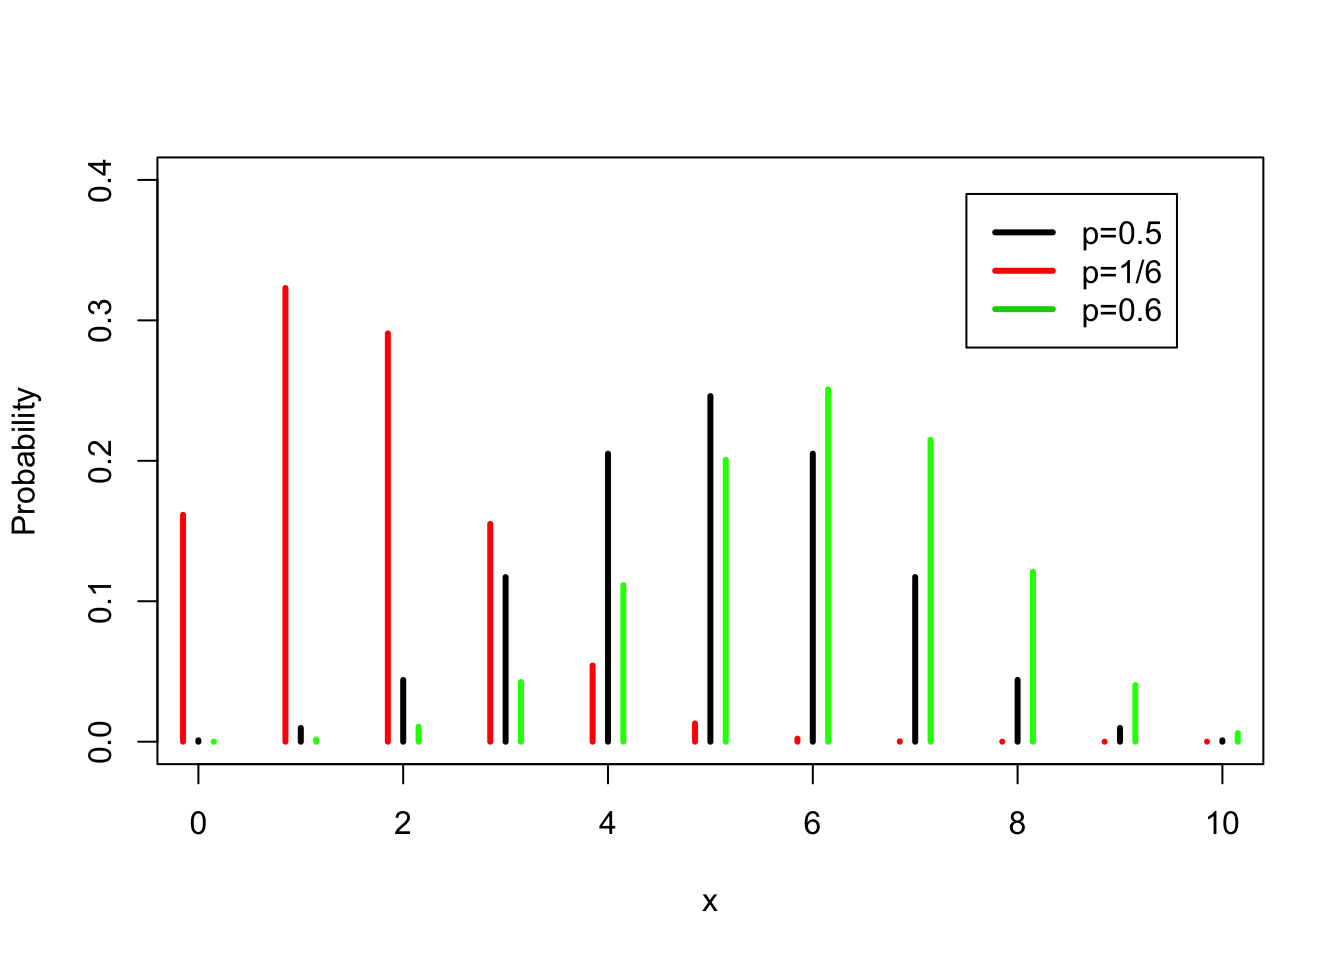
\includegraphics[width=0.6\linewidth]{statthink_files/figure-latex/RVar3-1} 

}

\caption{The Binomial Distribution for Various Probability of "Success"" $p$}\label{fig:RVar3}
\end{figure}

In Figure~\ref{fig:RVar3} the probabilities for
\(\mathrm{Binomial}(10,1/6)\), the \(\mathrm{Binomial}(10,1/2)\), and the
\(\mathrm{Binomial}(10,0.6)\) distributions are plotted side by side. In
all these 3 distributions the sample space is the same, the integers
between 0 and 10. However, the probabilities of the different values
differ. (Note that all bars should be placed on top of the integers. For
clarity of the presentation, the bars associated with the
\(\mathrm{Binomial}(10,1/6)\) are shifted slightly to the left and the
bars associated with the \(\mathrm{Binomial}(10,0.6)\) are shifted
slightly to the right.)

The expectation of the \(\mathrm{Binomial}(10,0.5)\) distribution is equal
to \(10 \times 0.5 = 5\). Compare this to the expectation of the
\(\mathrm{Binomial}(10,1/6)\) distribution, which is
\(10 \times (1/6) = 1.666667\) and to the expectation of the
\(\mathrm{Binomial}(10,0.6)\) distribution which equals
\(10 \times 0.6 = 6\).

The variance of the \(\mathrm{Binomial}(10,0.5)\) distribution is
\(10 \times 0.5 \times 0.5 = 2.5\). The variance when \(p=1/6\) is
\(10 \times (1/6) \times (5/6) = 1.388889\) and the variance when \(p=0.6\)
is \(10 \times 0.6 \times 0.4 = 2.4\).

\BeginKnitrBlock{example}
\protect\hypertarget{exm:exrvar1}{}{\label{exm:exrvar1} }As an application of the Binomial distribution
consider a pre-election poll. A candidate is running for office and is
interested in knowing the percentage of support in the general
population in its candidacy. Denote the probability of support by \(p\).
In order to estimate the percentage a sample of size 300 is selected
from the population. Let \(X\) be the count of supporters in the sample. A
natural model for the distribution of \(X\) is the
\(\mathrm{Binomial}(300,p)\) distribution, since each subject in the
sample may be a supporter (``Success'') or may not be a supporter
(``Failure''). The probability that a subject supports the candidate is
\(p\) and there are \(n=300\) subjects in the sample.
\EndKnitrBlock{example}

\BeginKnitrBlock{example}
\protect\hypertarget{exm:exrvar2}{}{\label{exm:exrvar2} }As another example consider the procedure for
quality control that is described in Discussion Forum of
Chapter~\ref{ChapProbability}. According to the procedure 20 items are
tested and the number of faulty items is recorded. If \(p\) is the
probability that an item is identified as faulty then the distribution
of the total number of faulty items may be modeled by the
\(\mathrm{Binomial}(20,p)\) distribution.
\EndKnitrBlock{example}

In both examples one may be interested in making statements on the
probability \(p\) based on the sample. Statistical inference relates the
actual count obtained in the sample to the theoretical Binomial
distribution in order to make such statements.

\hypertarget{the-poisson-random-variable}{%
\subsection{The Poisson Random Variable}\label{the-poisson-random-variable}}

The \emph{Poisson} distribution is used as an approximation of the total
number of occurrences of rare events. Consider, for example, the
Binomial setting that involves \(n\) trials with \(p\) as the probability of
success of each trial. Then, if \(p\) is small but \(n\) is large then the
number of successes \(X\) has, approximately, the Poisson distribution.

The sample space of the Poisson random variable is the unbounded
collection of integers: \(\{0,1,2, \ldots\}\). Any integer value is
assigned a positive probability. Hence, the Poisson random variable is a
convenient model when the maximal number of occurrences of the events in
a-priori unknown or is very large. For example, one may use the Poisson
distribution to model the number of phone calls that enter a switchboard
in a given interval of time or the number of malfunctioning components
in a shipment of some product.

\begin{figure}

{\centering 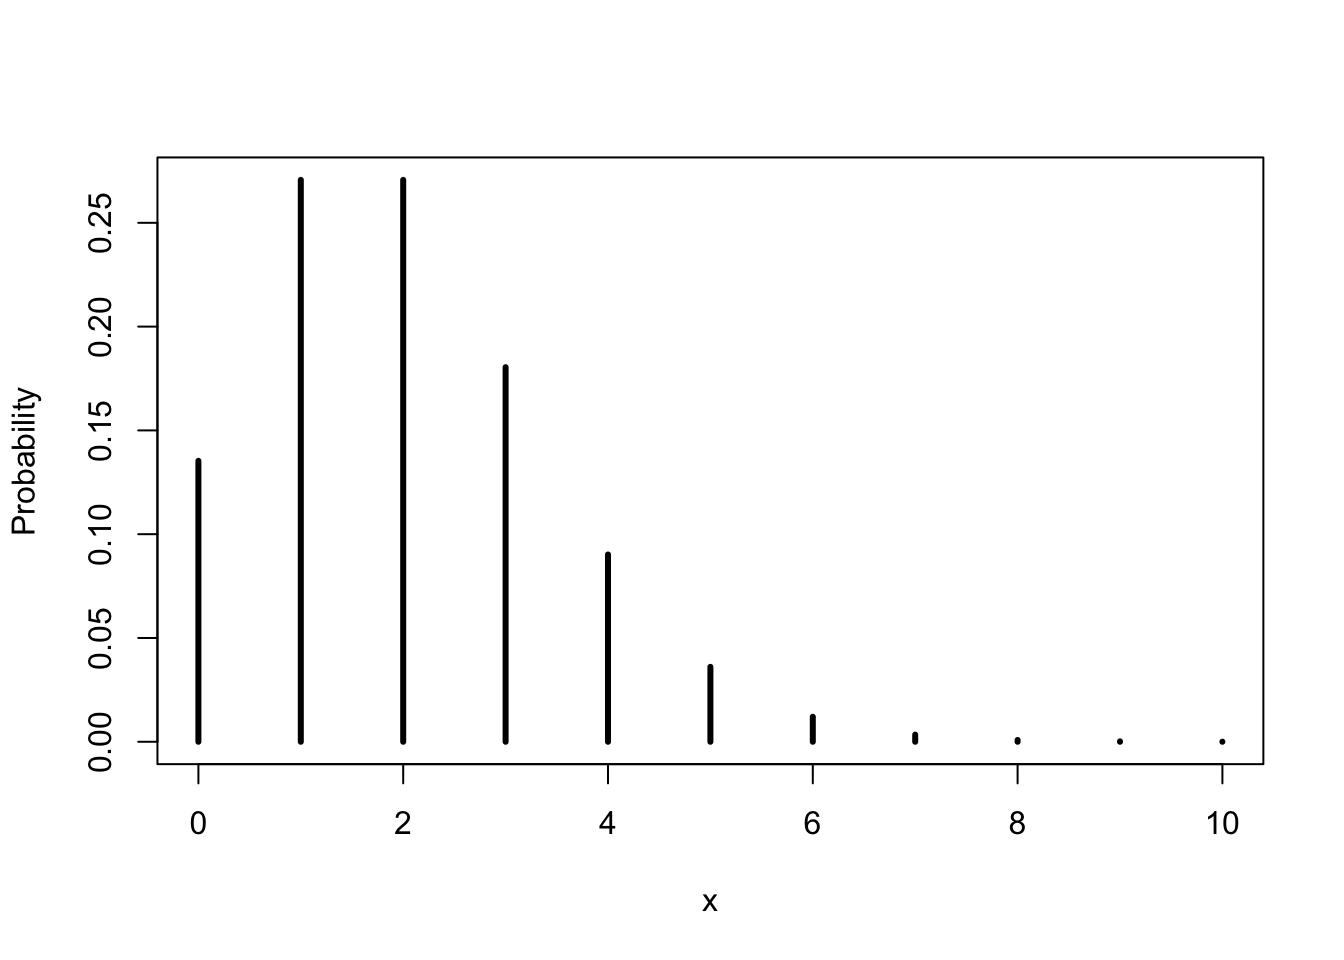
\includegraphics[width=0.6\linewidth]{statthink_files/figure-latex/RVar4-1} 

}

\caption{The Poisson(2) Distribution}\label{fig:RVar4}
\end{figure}

The Binomial distribution was specified by the number of trials \(n\) and
probability of success in each trial \(p\). The Poisson distribution is
specified by its expectation, which we denote by \(\lambda\). The
expression ``\(X \sim \mathrm{Poisson}(\lambda)\)'' states that the random
variable \(X\) has a Poisson distribution\footnote{If \(X \sim \mathrm{Poisson}(\lambda)\) then
  \(\Prob(X=x) = e^{-\lambda}\lambda^x/x!\), for \(x=0,1,2,\ldots\).} with expectation
\(\Expec(X) = \lambda\). The function ``\texttt{dpois}'' computes the probability,
according to the Poisson distribution, of values that are entered as the
first argument to the function. The expectation of the distribution is
entered in the second argument. The function ``\texttt{ppois}'' computes the
cumulative probability. Consequently, we can compute the probabilities
and the cumulative probabilities of the values between 0 and 10 for the
\(\mathrm{Poisson}(2)\) distribution via:

\begin{Shaded}
\begin{Highlighting}[]
\NormalTok{x <-}\StringTok{ }\DecValTok{0}\OperatorTok{:}\DecValTok{10}
\KeywordTok{dpois}\NormalTok{(x,}\DecValTok{2}\NormalTok{)}
\end{Highlighting}
\end{Shaded}

\begin{verbatim}
##  [1] 0.135335283237 0.270670566473 0.270670566473 0.180447044315
##  [5] 0.090223522158 0.036089408863 0.012029802954 0.003437086558
##  [9] 0.000859271640 0.000190949253 0.000038189851
\end{verbatim}

\begin{Shaded}
\begin{Highlighting}[]
\KeywordTok{ppois}\NormalTok{(x,}\DecValTok{2}\NormalTok{)}
\end{Highlighting}
\end{Shaded}

\begin{verbatim}
##  [1] 0.13533528 0.40600585 0.67667642 0.85712346 0.94734698 0.98343639
##  [7] 0.99546619 0.99890328 0.99976255 0.99995350 0.99999169
\end{verbatim}

The probability function of the Poisson distribution with \(\lambda = 2\),
in the range between 0 and 10, is plotted in
Figure~\ref{fig:RVar4}. Observe that in this example probabilities
of the values 8 and beyond are very small. As a matter of fact, the
cumulative probability at \(x=7\) (the 8th value in the output of
``\texttt{ppois(x,2)}'') is approximately 0.999, out of the total cumulative
probability of 1.000, leaving a total probability of about 0.001 to be
distributed among all the values larger than 7.

\begin{figure}

{\centering 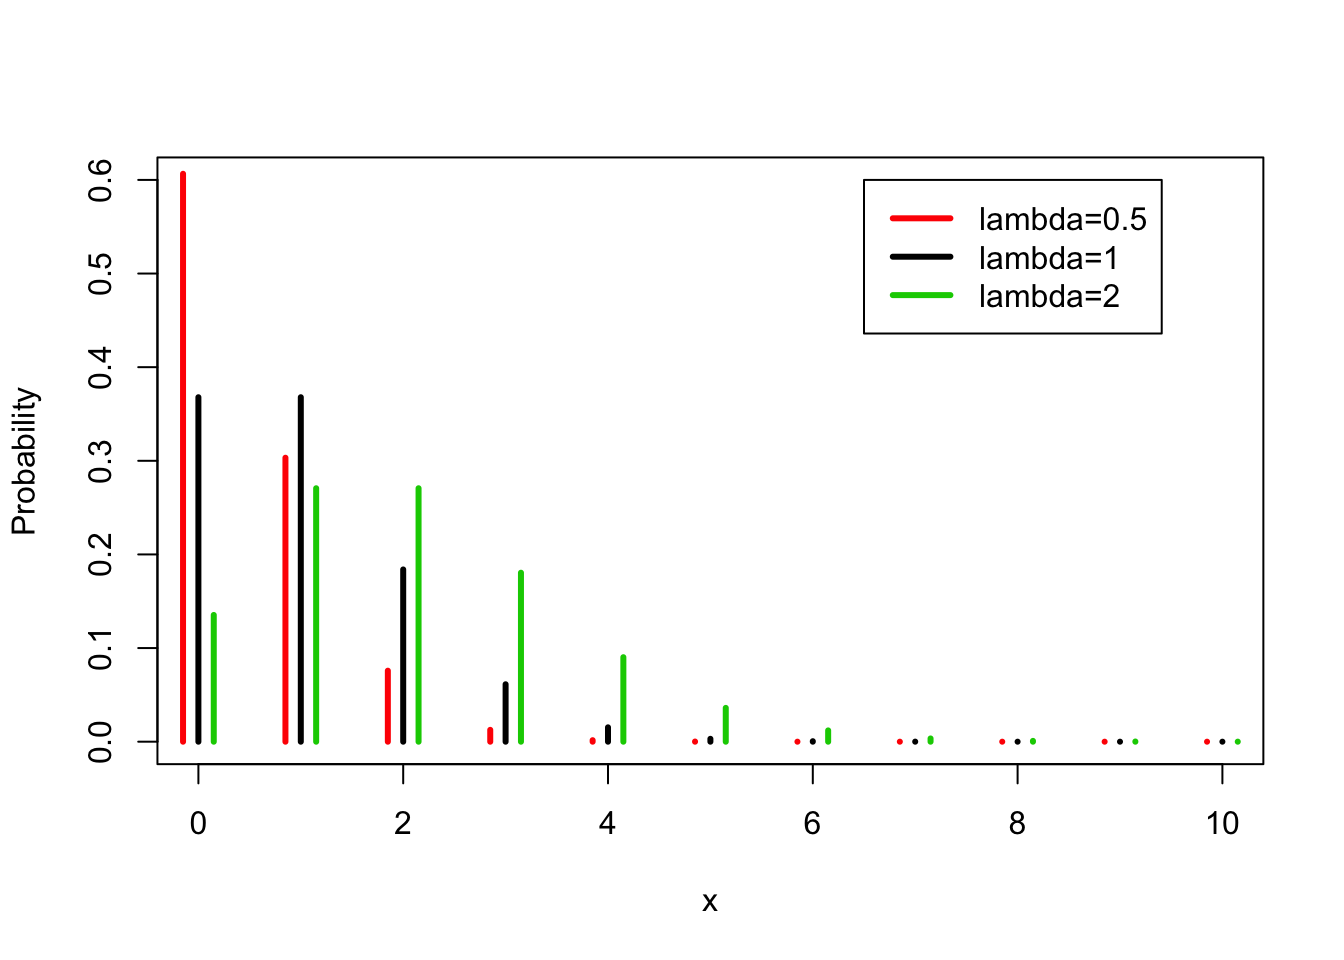
\includegraphics[width=0.6\linewidth]{statthink_files/figure-latex/RVar5-1} 

}

\caption{The Poisson Distribution for Various Values of $\lambda$}\label{fig:RVar5}
\end{figure}

Let us compute the expectation of the given Poisson distribution:

\begin{Shaded}
\begin{Highlighting}[]
\NormalTok{X.val <-}\StringTok{ }\DecValTok{0}\OperatorTok{:}\DecValTok{10}
\NormalTok{P.val <-}\StringTok{ }\KeywordTok{dpois}\NormalTok{(X.val,}\DecValTok{2}\NormalTok{)}
\KeywordTok{sum}\NormalTok{(X.val}\OperatorTok{*}\NormalTok{P.val)}
\end{Highlighting}
\end{Shaded}

\begin{verbatim}
## [1] 1.999907
\end{verbatim}

Observe that the outcome is almost, but not quite, equal to \(2.00\),
which is the actual value of the expectation. The reason for the
inaccuracy is the fact that we have based the computation in \texttt{R} on the
first 11 values of the distribution only, instead of the infinite
sequence of values. A more accurate result may be obtained by the
consideration of the first 101 values:

\begin{Shaded}
\begin{Highlighting}[]
\NormalTok{X.val <-}\StringTok{ }\DecValTok{0}\OperatorTok{:}\DecValTok{100}
\NormalTok{P.val <-}\StringTok{ }\KeywordTok{dpois}\NormalTok{(X.val,}\DecValTok{2}\NormalTok{)}
\NormalTok{EX <-}\StringTok{ }\KeywordTok{sum}\NormalTok{(X.val}\OperatorTok{*}\NormalTok{P.val)}
\NormalTok{EX}
\end{Highlighting}
\end{Shaded}

\begin{verbatim}
## [1] 2
\end{verbatim}

\begin{Shaded}
\begin{Highlighting}[]
\KeywordTok{sum}\NormalTok{((X.val}\OperatorTok{-}\NormalTok{EX)}\OperatorTok{^}\DecValTok{2}\OperatorTok{*}\NormalTok{P.val)}
\end{Highlighting}
\end{Shaded}

\begin{verbatim}
## [1] 2
\end{verbatim}

In the last expression we have computed the variance of the Poisson
distribution and obtained that it is equal to the expectation. This
results can be validated mathematically. For the Poisson distribution it
is always the case that the variance is equal to the expectation, namely
to \(\lambda\): \[\Expec(X) = \Var(X) = \lambda\;.\]

In Figure~\ref{fig:RVar5} you may find the probabilities of the
Poisson distribution for \(\lambda = 0.5\), \(\lambda = 1\) and
\(\lambda = 2\). Notice once more that the sample space is the same for
all the Poisson distributions. What varies when we change the value of
\(\lambda\) are the probabilities. Observe that as \(\lambda\) increases
then probability of larger values increases as well.

\BeginKnitrBlock{example}
\protect\hypertarget{exm:exrvar3}{}{\label{exm:exrvar3} }A radio active element decays by the release of
subatomic particles and energy. The decay activity is measured in terms
of the number of decays per second in a unit mass. A typical model for
the distribution of the number of decays is the Poisson distribution.
Observe that the number of decays in a second is a integer and, in
principle, it may obtain any integer value larger or equal to zero. The
event of a radio active decay of an atom is a relatively rare event.
Therefore, the Poisson model is likely to fit this phenomena\footnote{The number of decays may also be considered in the
  \(\mathrm{Binomial}(n,p)\) setting. The number \(n\) is the total number
  of atoms in the unit mass and \(p\) is the probability that an atom
  decays within the given second. However, since \(n\) is very large and
  \(p\) is very small we get that the Poisson distribution is an
  appropriate model for the count.}.
\EndKnitrBlock{example}

\BeginKnitrBlock{example}
\protect\hypertarget{exm:exrvar4}{}{\label{exm:exrvar4} }Consider an overhead power line suspended between
two utility poles. During rain, drops of water may hit the power line.
The total number of drops that hit the line in a one minute period may
be modeled by a Poisson random variable.
\EndKnitrBlock{example}

\hypertarget{RandomVar_5}{%
\section{Continuous Random Variable}\label{RandomVar_5}}

Many types of measurements, such as height, weight, angle, temperature,
etc., may in principle have a continuum of possible values. Continuous
random variables are used to model uncertainty regarding future values
of such measurements.

The main difference between discrete random variables, which is the type
we examined thus far, and continuous random variable, that are added now
to the list, is in the sample space, i.e., the collection of possible
outcomes. The former type is used when the possible outcomes are
separated from each other as the integers are. The latter type is used
when the possible outcomes are the entire line of real numbers or when
they form an interval (possibly an open ended one) of real numbers.

The difference between the two types of sample spaces implies
differences in the way the distribution of the random variables is being
described. For discrete random variables one may list the probability
associated with each value in the sample space using a table, a formula,
or a bar plot. For continuous random variables, on the other hand,
probabilities are assigned to intervals of values, and not to specific
values. Thence, densities are used in order to display the distribution.

Densities are similar to histograms, with areas under the plot
corresponding to probabilities. We will provide a more detailed
description of densities as we discuss the different examples of
continuous random variables.

In continuous random variables integration replaces summation and the
density replaces the probability in the computation of quantities such
as the probability of an event, the expectation, and the variance.

Hence, if the expectation of a discrete random variable is given in the
formula \(\Expec(X) = \sum_x \big(x \times \Prob(x)\big)\), which involves
the summation over all values of the product between the value and the
probability of the value, then for continuous random variable the
definition becomes:

\[\Expec(X) = \int \big(x \times f(x)\big)dx\;,\]
where \(f(x)\) is the density of \(X\) at the value \(x\). Therefore, in the
expectation of a continuous random variable one multiplies the value by
the density at the value. This product is then integrated over the
sample space.

Likewise, the formula
\(\Var(X) = \sum_x\big( (x-\Expec(X))^2 \times \Prob(x)\big)\) for the
variance is replaced by:

\[\Var(X) =\int\big((x-\Expec(X))^2 \times f(x) \big) dx\;.\]
Nonetheless, the intuitive interpretation of the expectation as the
central value of the distribution that identifies the location and the
interpretation of the standard deviation (the square root of the
variance) as the summary of the total spread of the distribution is
still valid.

In this section we will describe two types of continuous random
variables: Uniform and Exponential. In the next chapter another example
-- the Normal distribution -- will be introduced.

\hypertarget{the-uniform-random-variable}{%
\subsection{The Uniform Random Variable}\label{the-uniform-random-variable}}

The Uniform distribution is used in order to model measurements that may
have values in a given interval, with all values in this interval
equally likely to occur.

For example, consider a random variable \(X\) with the Uniform
distribution over the interval \([3,7]\), denoted by
``\(X \sim \mathrm{Uniform}(3,7)\)''. The density function at given values
may be computed with the aid of the function ``\texttt{dunif}''. For instance let
us compute the density of the \(\mathrm{Uniform}(3,7)\) distribution over
the integers \(\{0, 1, \ldots, 10\}\):

\begin{Shaded}
\begin{Highlighting}[]
\KeywordTok{dunif}\NormalTok{(}\DecValTok{0}\OperatorTok{:}\DecValTok{10}\NormalTok{,}\DecValTok{3}\NormalTok{,}\DecValTok{7}\NormalTok{)}
\end{Highlighting}
\end{Shaded}

\begin{verbatim}
##  [1] 0.00 0.00 0.00 0.25 0.25 0.25 0.25 0.25 0.00 0.00 0.00
\end{verbatim}

Notice that for the values 0, 1, and 2, and the values 8, 9 and 10 that
are outside of the interval the density is equal to zero, indicating
that such values cannot occur in the given distribution. The values of
the density at integers inside the interval are positive and equal to
each other. The density is not restricted to integer values. For
example, at the point \(4.73\) we get that the density is positive and of
the same height:

\begin{Shaded}
\begin{Highlighting}[]
\KeywordTok{dunif}\NormalTok{(}\FloatTok{4.73}\NormalTok{,}\DecValTok{3}\NormalTok{,}\DecValTok{7}\NormalTok{)}
\end{Highlighting}
\end{Shaded}

\begin{verbatim}
## [1] 0.25
\end{verbatim}

\begin{figure}

{\centering 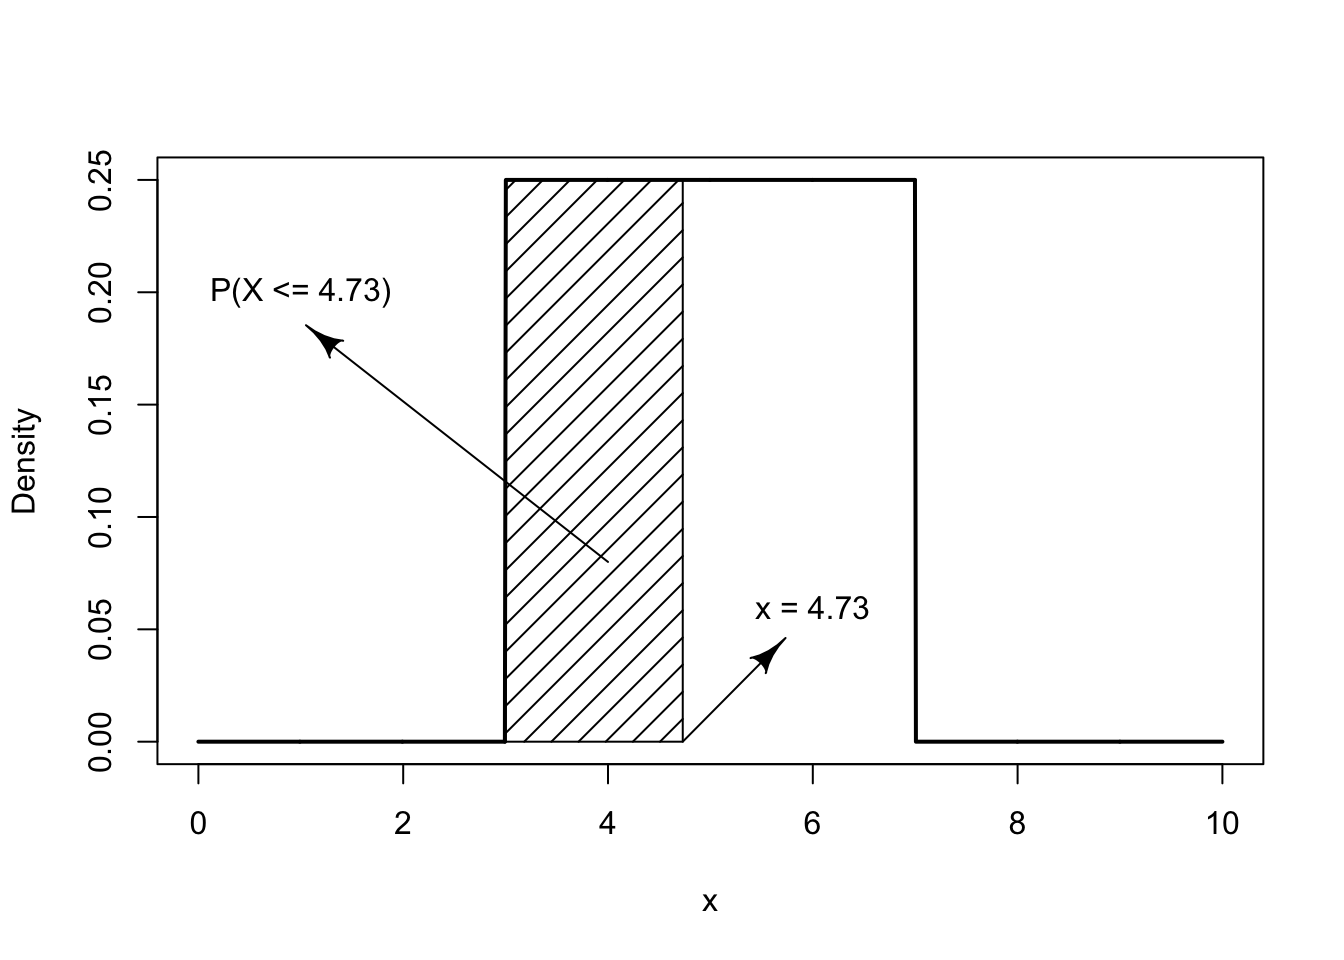
\includegraphics[width=0.6\linewidth]{statthink_files/figure-latex/RVar6-1} 

}

\caption{The Uniform(3,7) Distribution}\label{fig:RVar6}
\end{figure}

A plot of the \(\mathrm{Uniform}(3,7)\) density is given in
Figure~\ref{fig:RVar6} in the form of a solid line. Observe that
the density is positive over the interval \([3,7]\) where its height is
1/4. Area under the curve in the density corresponds to probability.
Indeed, the fact that the total probability is one is reflected in the
total area under the curve being equal to 1. Over the interval \([3,7]\)
the density forms a rectangle. The base of the rectangle is the length
of the interval \(7-3=4\). The height of the rectangle is thus equal to
1/4 in order to produce a total area of \(4 \times (1/4) = 1\).

The function ``\texttt{punif}'' computes the cumulative probability of the
uniform distribution. The probability \(\Prob(X \leq 4.73)\), for
\(X \sim \mathrm{Uniform}(3,7)\), is given by:

\begin{Shaded}
\begin{Highlighting}[]
\KeywordTok{punif}\NormalTok{(}\FloatTok{4.73}\NormalTok{,}\DecValTok{3}\NormalTok{,}\DecValTok{7}\NormalTok{)}
\end{Highlighting}
\end{Shaded}

\begin{verbatim}
## [1] 0.4325
\end{verbatim}

This probability corresponds to the marked area to the left of the point
\(x = 4.73\) in Figure~\ref{fig:RVar6}. This area of the marked
rectangle is equal to the length of the base 4.73 - 3 = 1.73, times the
height of the rectangle 1/(7-3) = 1/4. Indeed:

\begin{Shaded}
\begin{Highlighting}[]
\NormalTok{(}\FloatTok{4.73}\DecValTok{-3}\NormalTok{)}\OperatorTok{/}\NormalTok{(}\DecValTok{7-3}\NormalTok{)}
\end{Highlighting}
\end{Shaded}

\begin{verbatim}
## [1] 0.4325
\end{verbatim}

is the area of the marked rectangle and is equal to the probability.

Let us use \texttt{R} in order to plot the density and the cumulative
probability functions of the Uniform distribution. We produce first a
large number of points in the region we want to plot. The points are
produced with aid of the function ``\texttt{seq}''. The output of this function
is a sequence with equally spaced values. The starting value of the
sequence is the first argument in the input of the function and the last
value is the second argument in the input. The argument ``\texttt{length=1000}''
sets the length of the sequence, 1,000 values in this case:

\begin{Shaded}
\begin{Highlighting}[]
\NormalTok{x <-}\StringTok{ }\KeywordTok{seq}\NormalTok{(}\DecValTok{0}\NormalTok{,}\DecValTok{10}\NormalTok{,}\DataTypeTok{length=}\DecValTok{1000}\NormalTok{)}
\NormalTok{den <-}\StringTok{ }\KeywordTok{dunif}\NormalTok{(x,}\DecValTok{3}\NormalTok{,}\DecValTok{7}\NormalTok{)}
\KeywordTok{plot}\NormalTok{(x,den)}
\end{Highlighting}
\end{Shaded}

\begin{center}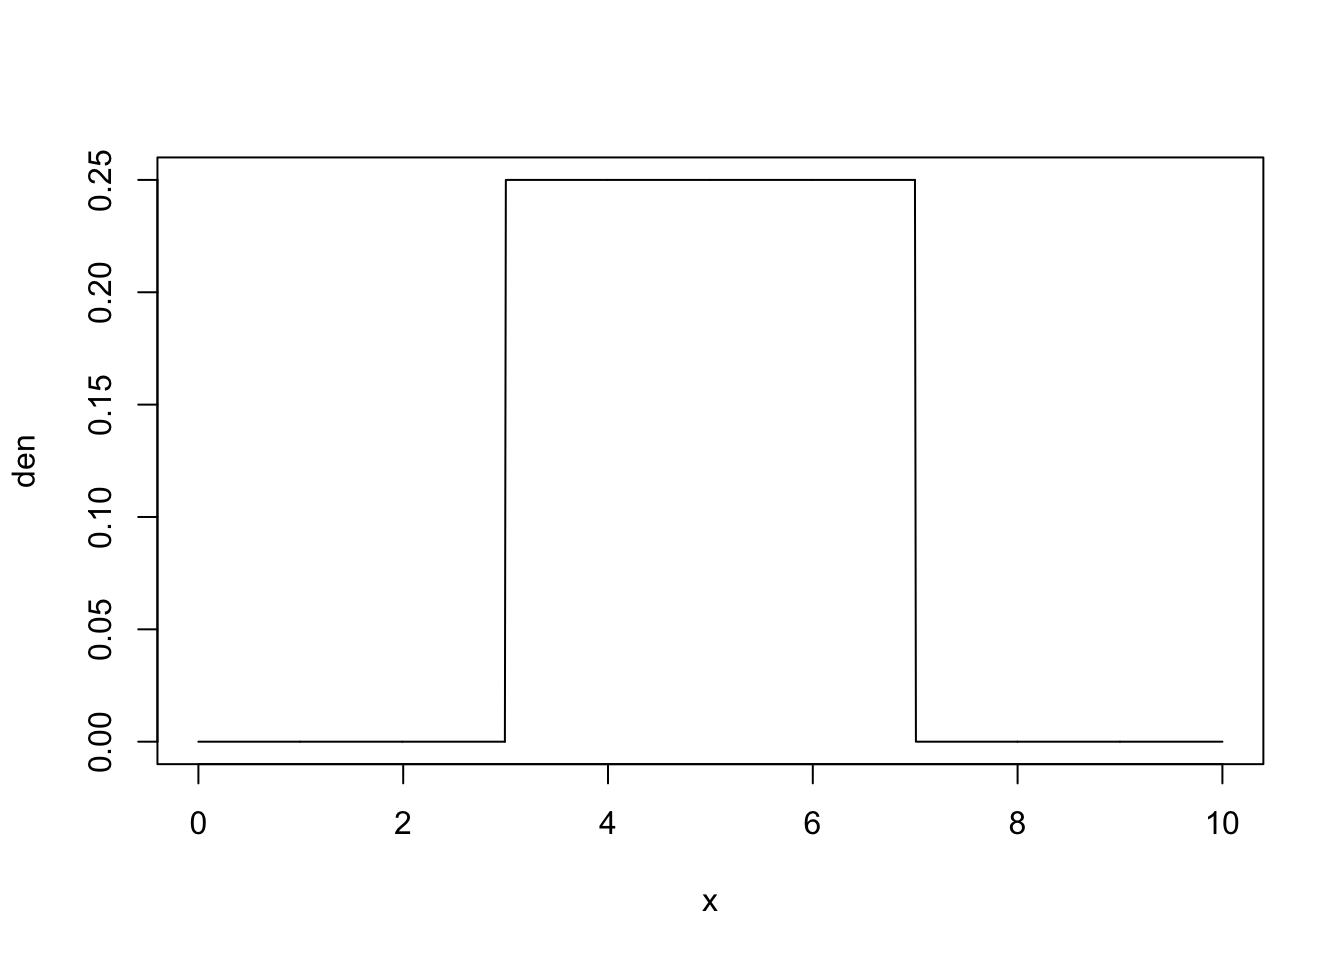
\includegraphics[width=0.6\linewidth]{statthink_files/figure-latex/unnamed-chunk-65-1} \end{center}

The object ``\texttt{den}'' is a sequence of length 1,000 that contains the
density of the \(\mathrm{Uniform}(3,7)\) evaluated over the values of
``\texttt{x}''. When we apply the function ``\texttt{plot}'' to the two sequences we get a
scatter plot of the 1,000 points.

A scatter plot is a plot of points. Each point in the scatter plot is
identify by its horizontal location on the plot (its ``\(x\)'' value) and by
its vertical location on the plot (its \(y\) value). The horizontal value
of each point in the plot is determined by the first argument to the
function ``\texttt{plot}'' and the vertical value is determined by the second
argument. For example, the first value in the sequence ``\texttt{x}'' is 0. The
value of the Uniform density at this point is 0. Hence, the first value
of the sequence ``\texttt{den}'' is also 0. A point that corresponds to these
values is produced in the plot. The horizontal value of the point is 0
and the vertical value is 0. In a similar way the other 999 points are
plotted. The last point to be plotted has a horizontal value of 10 and a
vertical value of 0.

The number of points that are plotted is large and they overlap each
other in the graph and thus produce an impression of a continuum. In
order to obtain nicer looking plots we may choose to connect the points
to each other with segments and use smaller points. This may be achieved
by the addition of the argument ``\texttt{type=l}'', with the letter \texttt{l} for
line, to the plotting function:

\begin{Shaded}
\begin{Highlighting}[]
\KeywordTok{plot}\NormalTok{(x,den,}\DataTypeTok{type=}\StringTok{"l"}\NormalTok{)}
\end{Highlighting}
\end{Shaded}

\begin{center}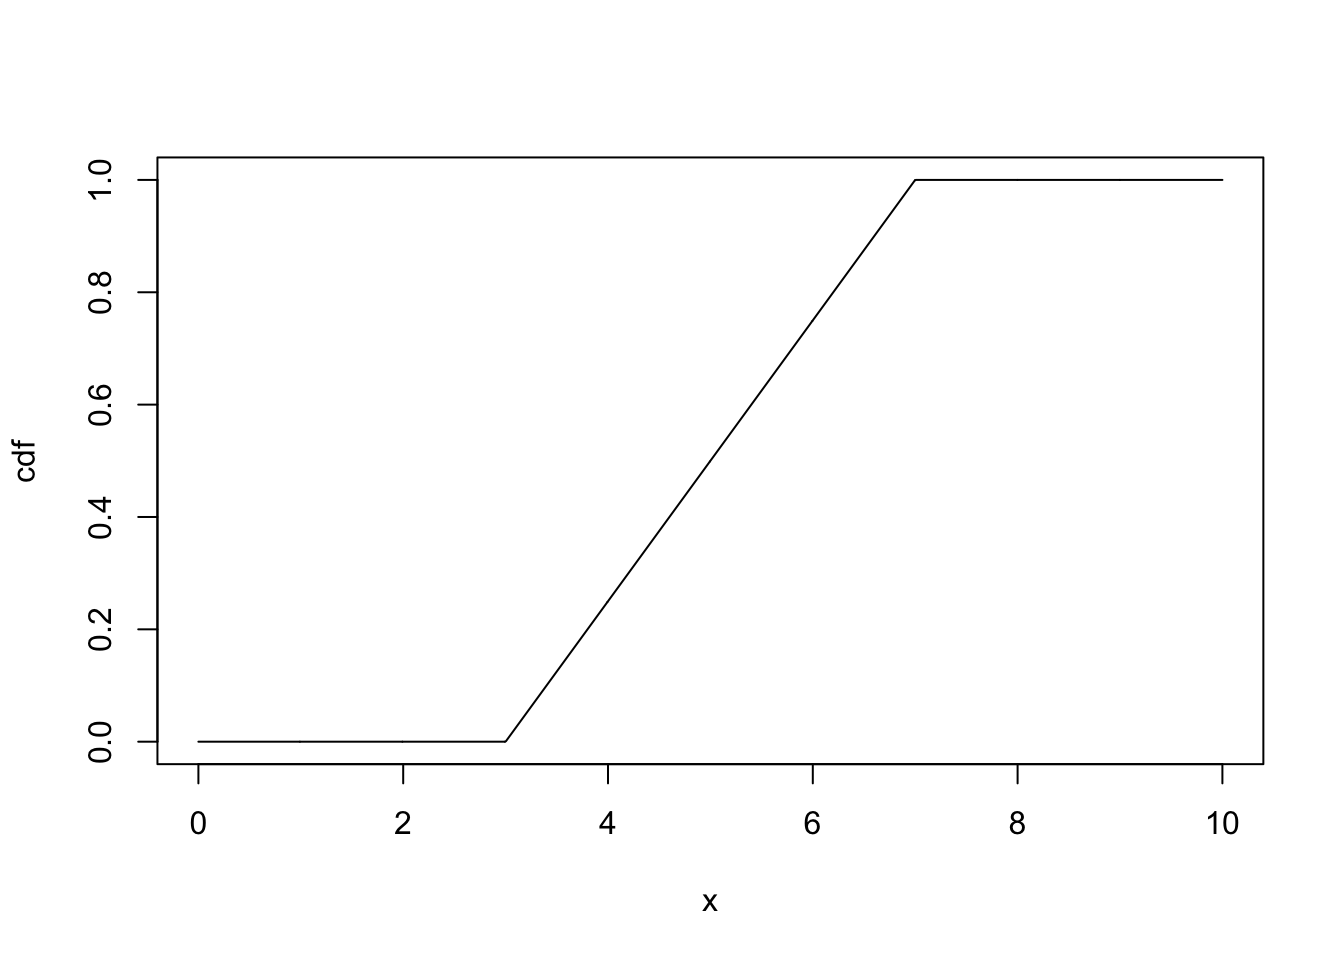
\includegraphics[width=0.6\linewidth]{statthink_files/figure-latex/unnamed-chunk-66-1} \end{center}

The cumulative probability of the \(\mathrm{Uniform}(3,7)\) is produced by the code:

\begin{Shaded}
\begin{Highlighting}[]
\NormalTok{cdf <-}\StringTok{ }\KeywordTok{punif}\NormalTok{(x,}\DecValTok{3}\NormalTok{,}\DecValTok{7}\NormalTok{)}
\KeywordTok{plot}\NormalTok{(x,cdf,}\DataTypeTok{type=}\StringTok{"l"}\NormalTok{)}
\end{Highlighting}
\end{Shaded}

\begin{center}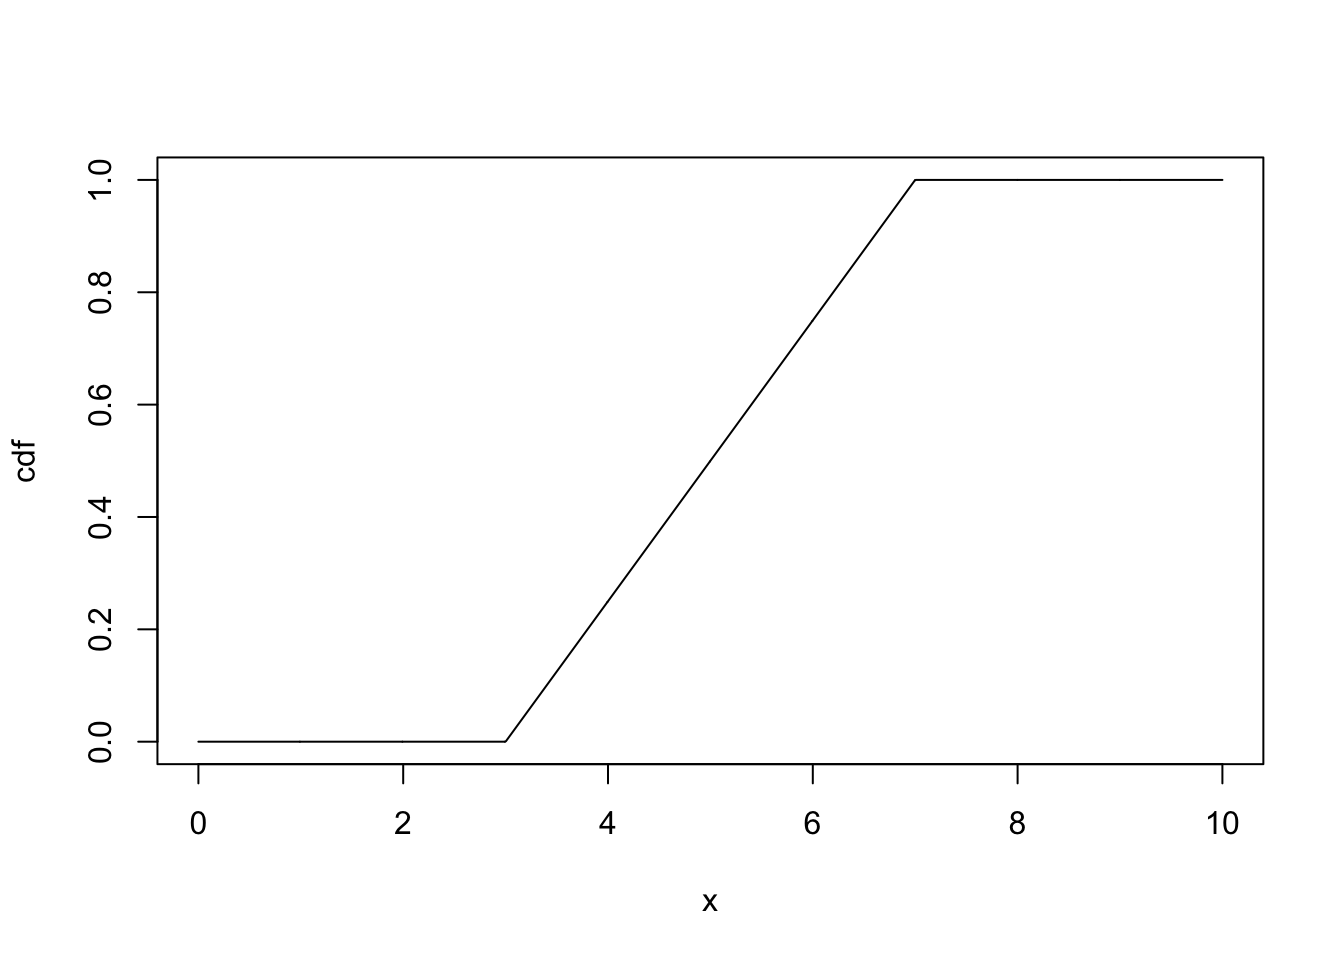
\includegraphics[width=0.6\linewidth]{statthink_files/figure-latex/unnamed-chunk-67-1} \end{center}

One can think of the density of the Uniform as an histogram\footnote{If \(X \sim \mathrm{Uniform}(a,b)\) then the density is
  \(f(x) = 1/(b-a)\), for \(a \leq x \leq b\), and it is equal to 0 for
  other values of \(x\).}. The
expectation of a Uniform random variable is the middle point of it's
histogram. Hence, if \(X \sim \mathrm{Uniform}(a,b)\) then:

\[\Expec(X) = \frac{a+b}{2}\;.\] For the \(X \sim \mathrm{Uniform}(3,7)\)
distribution the expectation is \(\Expec(X)= (3+7)/2 = 5\). Observe that 5
is the center of the Uniform density in Plot~\ref{fig:RVar6}.

It can be shown that the variance of the \(\mathrm{Uniform}(a,b)\) is
equal to

\[\Var(X) = \frac{(b-a)^2}{12}\;,\] with the standard deviation
being the square root of this value. Specifically, for
\(X \sim \mathrm{Uniform}(3,7)\) we get that
\(\Var(X) = (7-3)^2/12 = 1.333333\). The standard deviation is equal to
\(\sqrt{1.333333} = 1.154701\).

\BeginKnitrBlock{example}
\protect\hypertarget{exm:exrvar5}{}{\label{exm:exrvar5} }In Example~\ref{exm:exrvar4} we considered
rain drops that hit an overhead power line suspended between two utility
poles. The {\textbf{number}} of drops that hit the line can be modeled
using the Poisson distribution. The {\textbf{position}} between the two
poles where a rain drop hits the line can be modeled by the Uniform
distribution. The rain drop can hit any position between the two utility
poles. Hitting one position along the line is as likely as hitting any
other position.
\EndKnitrBlock{example}

\BeginKnitrBlock{example}
\protect\hypertarget{exm:exrvar6}{}{\label{exm:exrvar6} }Meiosis is the process in which a diploid cell
that contains two copies of the genetic material produces an haploid
cell with only one copy (sperms or eggs, depending on the sex). The
resulting molecule of genetic material is linear molecule (chromosome)
that is composed of consecutive segments: a segment that originated from
one of the two copies followed by a segment from the other copy and vice
versa. The border points between segments are called points of
crossover. The Haldane model for crossovers states that the position of
a crossover between two given loci on the chromosome corresponds to the
Uniform distribution and the total number of crossovers between these
two loci corresponds to the Poisson distribution.
\EndKnitrBlock{example}

\hypertarget{the-exponential-random-variable}{%
\subsection{The Exponential Random Variable}\label{the-exponential-random-variable}}

The Exponential distribution is frequently used to model times between
events. For example, times between incoming phone calls, the time until
a component becomes malfunction, etc. We denote the Exponential
distribution via ``\(X \sim \mathrm{Exponential}(\lambda)\)'', where
\(\lambda\) is a parameter that characterizes the distribution and is
called the \emph{rate} of the distribution. The overlap between the parameter
used to characterize the Exponential distribution and the one used for
the Poisson distribution is deliberate. The two distributions are
tightly interconnected. As a matter of fact, it can be shown that if the
distribution between occurrences of a phenomena has the Exponential
distribution with rate \(\lambda\) then the total number of the
occurrences of the phenomena within a unit interval of time has a
\(\mathrm{Poisson}(\lambda)\) distribution.

The sample space of an Exponential random variable contains all
non-negative numbers. Consider, for example,
\(X \sim \mathrm{Exponential}(0.5)\). The density of the distribution in
the range between 0 and 10 is presented in Figure~\ref{fig:RVar7}.
Observe that in the Exponential distribution smaller values are more
likely to occur in comparison to larger values. This is indicated by the
density being larger at the vicinity of 0. The density of the
exponential distribution given in the plot is positive, but hardly so,
for values larger than 10.

\begin{figure}

{\centering 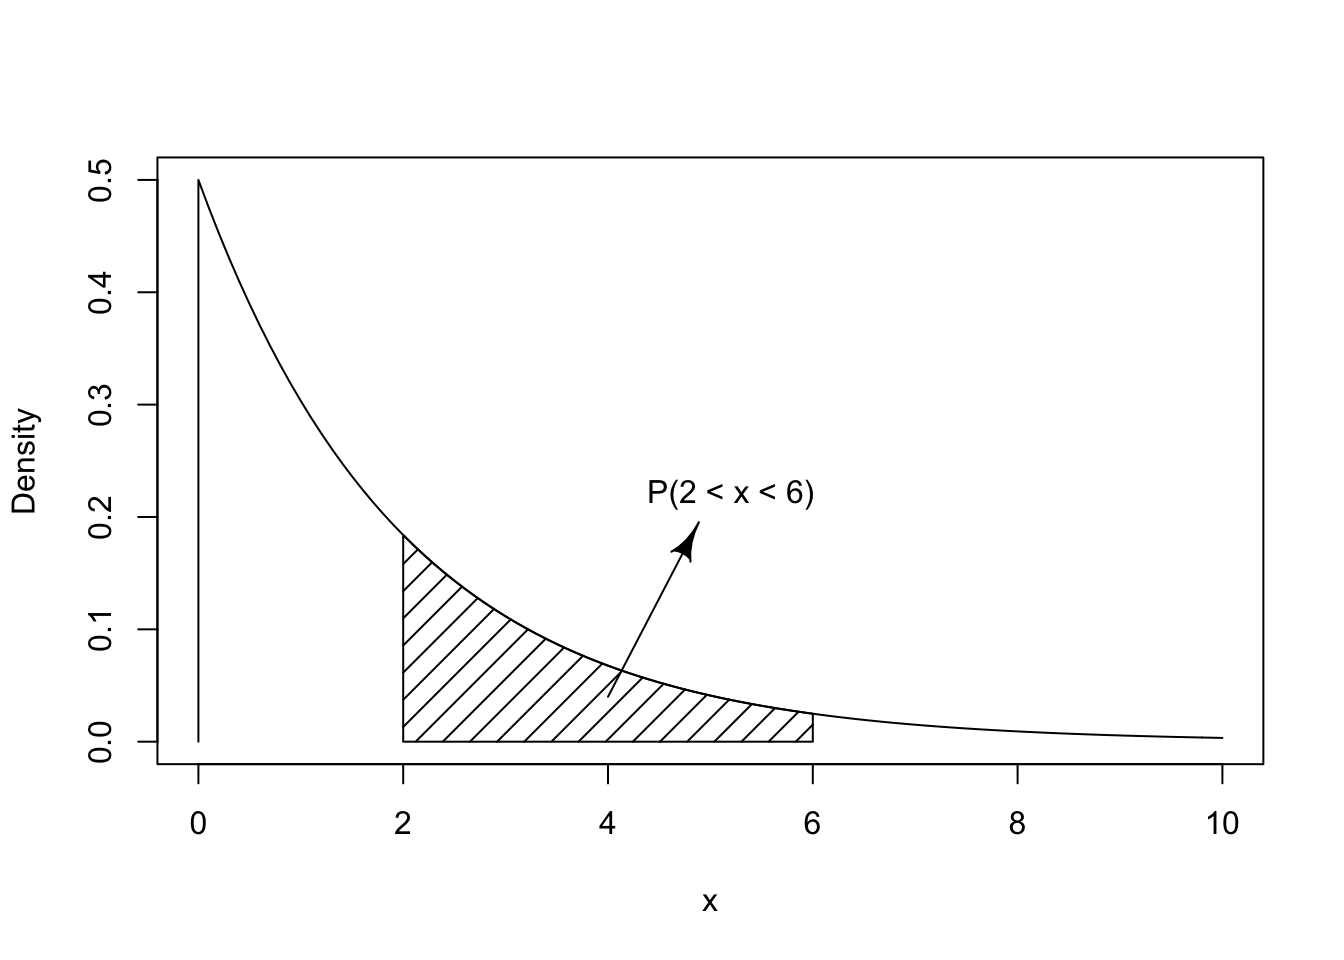
\includegraphics[width=0.6\linewidth]{statthink_files/figure-latex/RVar7-1} 

}

\caption{The Exponential(0.5) Distribution}\label{fig:RVar7}
\end{figure}

The density of the Exponential distribution can be computed with the aid
of the function ``\texttt{dexp}''\footnote{If \(X \sim \mathrm{Exponential}(\lambda)\) then the density
  is \(f(x) =\lambda e^{-\lambda x}\), for \(0 \leq x\), and it is equal
  to 0 for \(x < 0\).}. The cumulative probability can be computed
with the function ``\texttt{pexp}''. For illustration, assume
\(X \sim \mathrm{Exponential}(0.5)\). Say one is interested in the
computation of the probability \(\Prob(2 < X \leq 6)\) that the random
variable obtains a value that belongs to the interval \((2,6]\). The
required probability is indicated as the marked area in
Figure~\ref{fig:RVar7}. This area can be computed as the difference
between the probability \(\Prob(X \leq 6)\), the area to the left of 6,
and the probability \(\Prob(X \leq 2)\), the area to the left of 2:

\begin{Shaded}
\begin{Highlighting}[]
\KeywordTok{pexp}\NormalTok{(}\DecValTok{6}\NormalTok{,}\FloatTok{0.5}\NormalTok{) }\OperatorTok{-}\StringTok{ }\KeywordTok{pexp}\NormalTok{(}\DecValTok{2}\NormalTok{,}\FloatTok{0.5}\NormalTok{)}
\end{Highlighting}
\end{Shaded}

\begin{verbatim}
## [1] 0.31809237
\end{verbatim}

The difference is the probability of belonging to the interval, namely
the area marked in the plot.

The expectation of \(X\), when \(X \sim \mathrm{Exponential}(\lambda)\), is
given by the equation:

\[\Expec(X) = 1/\lambda\;,\] and the variance is
given by:

\[\Var(X) =1/\lambda^2\;.\] The standard deviation is the
square root of the variance, namely \(1/\lambda\). Observe that the larger
is the rate the smaller are the expectation and the standard deviation.

\begin{figure}

{\centering 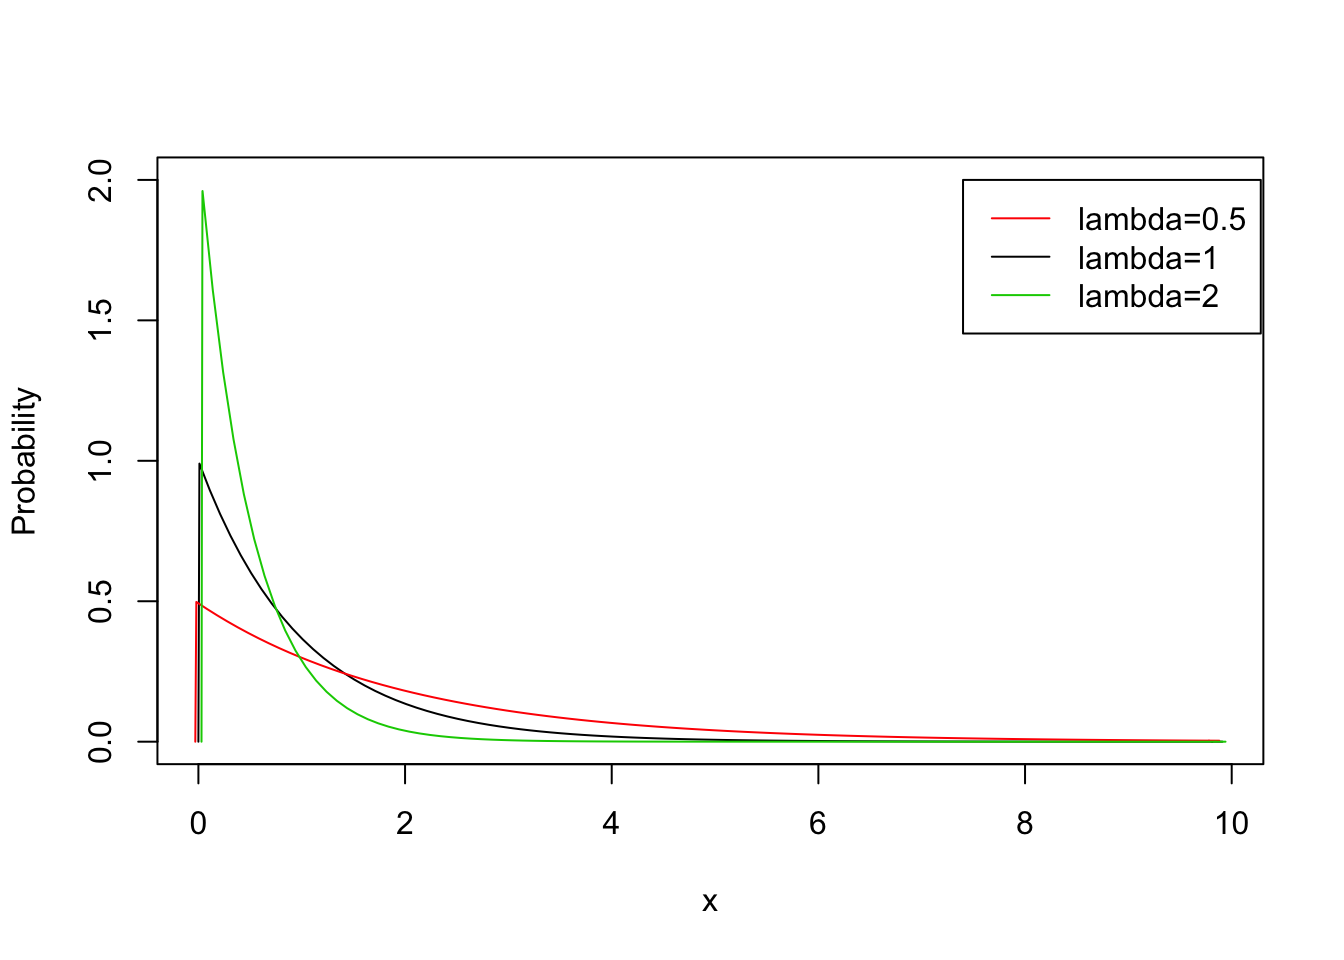
\includegraphics[width=0.6\linewidth]{statthink_files/figure-latex/RVar8-1} 

}

\caption{The Exponential Distribution for Various Values of $\lambda$}\label{fig:RVar8}
\end{figure}

In Figure~\ref{fig:RVar8} the densities of the Exponential
distribution are plotted for \(\lambda = 0.5\), \(\lambda = 1\), and
\(\lambda = 2\). Notice that with the increase in the value of the
parameter then the values of the random variable tends to become
smaller. This inverse relation makes sense in connection to the Poisson
distribution. Recall that the Poisson distribution corresponds to the
total number of occurrences in a unit interval of time when the time
between occurrences has an Exponential distribution. A larger
expectation \(\lambda\) of the Poisson corresponds to a larger number of
occurrences that are likely to take place during the unit interval of
time. The larger is the number of occurrences the smaller are the time
intervals between occurrences.

\BeginKnitrBlock{example}
\protect\hypertarget{exm:exrvar7}{}{\label{exm:exrvar7} }Consider Examples~\ref{exm:exrvar4}
and~\ref{exm:exrvar5} that deal with rain dropping on a power line.
The times between consecutive hits of the line may be modeled by the
Exponential distribution. Hence, the time to the first hit has an
Exponential distribution. The time between the first and the second hit
is also Exponentially distributed, and so on.
\EndKnitrBlock{example}

\BeginKnitrBlock{example}
\protect\hypertarget{exm:exrvar8}{}{\label{exm:exrvar8} }Return to Example~\ref{exm:exrvar3} that
deals with the radio activity of some element. The total count of decays
per second is model by the Poisson distribution. The times between radio
active decays is modeled according to the Exponential distribution. The
rate \(\lambda\) of that Exponential distribution is equal to the
expectation of the total count of decays in one second, i.e.~the
expectation of the Poisson distribution.
\EndKnitrBlock{example}

\hypertarget{sec:RVarExercises}{%
\section{Exercises}\label{sec:RVarExercises}}

\BeginKnitrBlock{exercise}
\protect\hypertarget{exr:unnamed-chunk-69}{}{\label{exr:unnamed-chunk-69} }A particular measles vaccine produces a reaction (a
fever higher that 102 Fahrenheit) in each vaccinee with probability of
0.09. A clinic vaccinates 500 people each day.

\begin{enumerate}
\def\labelenumi{\arabic{enumi}.}
\item
  What is the expected number of people that will develop a reaction
  each day?
\item
  What is the standard deviation of the number of people that will
  develop a reaction each day?
\item
  In a given day, what is the probability that more than 40 people
  will develop a reaction?
\item
  In a given day, what is the probability that the number of people
  that will develop a reaction is between 50 and 45 (inclusive)?
\end{enumerate}
\EndKnitrBlock{exercise}

\begin{figure}

{\centering 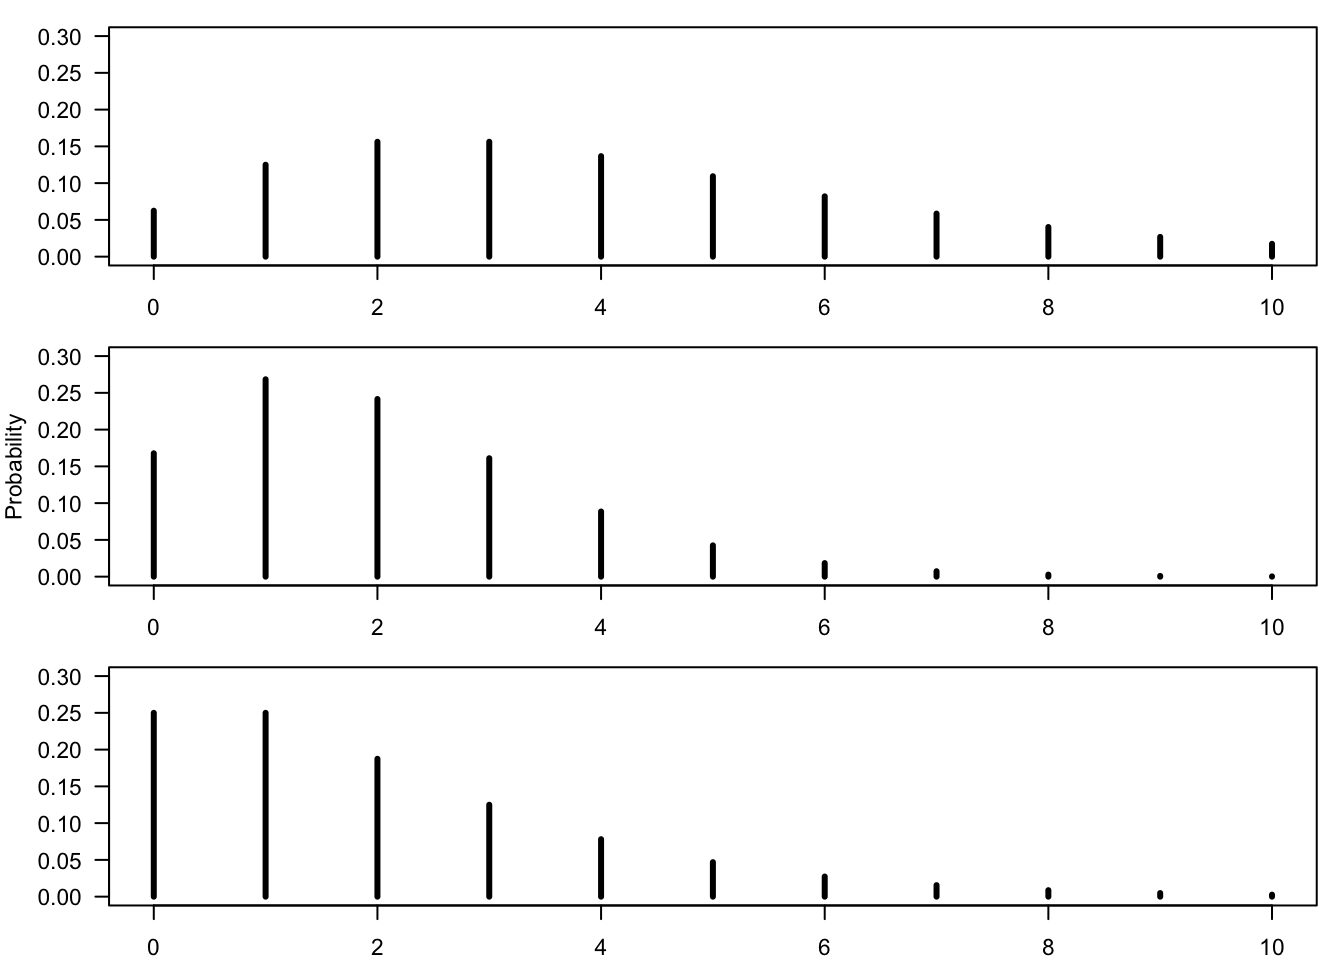
\includegraphics[width=0.6\linewidth]{statthink_files/figure-latex/RVar10-1} 

}

\caption{Bar Plots of the Negative-Binomial Distribution}\label{fig:RVar10}
\end{figure}

\BeginKnitrBlock{exercise}
\protect\hypertarget{exr:unnamed-chunk-70}{}{\label{exr:unnamed-chunk-70} }The Negative-Binomial distribution is yet another
example of a discrete, integer valued, random variable. The sample space
of the distribution are all non-negative integers \(\{0, 1, 2, \ldots\}\).
The fact that a random variable \(X\) has this distribution is marked by
``\(X \sim \mbox{Negative-Binomial}(r,p)\)'', where \(r\) and \(p\) are
parameters that specify the distribution.

Consider 3 random variables from the Negative-Binomial distribution:

\begin{itemize}
\item
  \(X_1 \sim \mbox{Negative-Binomial}(2,0.5)\)
\item
  \(X_2 \sim \mbox{Negative-Binomial}(4,0.5)\)
\item
  \(X_3 \sim \mbox{Negative-Binomial}(8,0.8)\)
\end{itemize}

The bar plots of these random variables are presented in
Figure~\ref{fig:RVar10}, re-organizer in a random order.

\begin{enumerate}
\def\labelenumi{\arabic{enumi}.}
\item
  Produce bar plots of the distributions of the random variables
  \(X_1\), \(X_2\), \(X_3\) in the range of integers between 0 and 15 and
  thereby identify the pair of parameters that produced each one of
  the plots in Figure~\ref{fig:RVar10}. Notice that the bar plots
  can be produced with the aid of the function ``\texttt{plot}'' and the
  function ``\texttt{dnbinom(x,r,p)}'', where ``\texttt{x}'' is a sequence of integers
  and ``\texttt{r}'' and ``\texttt{p}'' are the parameters of the distribution. Pay
  attention to the fact that you should use the argument ``\texttt{type\ =\ h}''
  in the function ``\texttt{plot}'' in order to produce the horizontal bars.
\item
  Below is a list of pairs that includes an expectation and a
  variance. Each of the pairs is associated with one of the random
  variables \(X_1\), \(X_2\), and \(X_3\):

  \begin{enumerate}
  \def\labelenumii{\arabic{enumii}.}
  \item
    \(\Expec(X) = 4\), \(\Var(X) = 8\).
  \item
    \(\Expec(X) = 2\), \(\Var(X) = 4\).
  \item
    \(\Expec(X) = 2\), \(\Var(X) = 2.5\).
  \end{enumerate}

  Use Figure~\ref{fig:RVar10} in order to match the random
  variable with its associated pair. Do not use numerical computations
  or formulae for the expectation and the variance in the
  Negative-Binomial distribution in order to carry out the
  matching\footnote{It can be shown, or else found on the web, that if
    \(X\sim \mbox{Negative-Binomial}(r,p)\) then \(\Expec(X) = r(1-p)/p\)
    and \(\Var(X) = r(1-p)/p^2\).}. Use, instead, the structure of the bar-plots.
\end{enumerate}
\EndKnitrBlock{exercise}

\hypertarget{summary-4}{%
\section{Summary}\label{summary-4}}

\hypertarget{glossary}{%
\subsection*{Glossary}\label{glossary}}


\begin{description}
\item[Binomial Random Variable:]
The number of successes among \(n\) repeats of independent trials with
a probability \(p\) of success in each trial. The distribution is
marked as \(\mathrm{Binomial}(n,p)\).
\item[Poisson Random Variable:]
An approximation to the number of occurrences of a rare event, when
the expected number of events is \(\lambda\). The distribution is
marked as \(\mathrm{Poisson}(\lambda)\).
\item[Density:]
Histogram that describes the distribution of a continuous random
variable. The area under the curve corresponds to probability.
\item[Uniform Random Variable:]
A model for a measurement with equally likely outcomes over an
interval \([a,b]\). The distribution is marked as
\(\mathrm{Uniform}(a,b)\).
\item[Exponential Random Variable:]
A model for times between events. The distribution is marked as
\(\mathrm{Exponential}(\lambda)\).
\end{description}

\hypertarget{discuss-in-the-forum}{%
\subsection*{Discuss in the Forum}\label{discuss-in-the-forum}}


This unit deals with two types of discrete random variables, the
Binomial and the Poisson, and two types of continuous random variables,
the Uniform and the Exponential. Depending on the context, these types
of random variables may serve as theoretical models of the uncertainty
associated with the outcome of a measurement.

In your opinion, is it or is it not useful to have a theoretical model
for a situation that occurs in real life?

When forming your answer to this question you may give an example of a
situation from you own field of interest for which a random variable,
possibly from one of the types that are presented in this unit, can
serve as a model. Discuss the importance (or lack thereof) of having a
theoretical model for the situation.

For example, the Exponential distribution may serve as a model for the
time until an atom of a radio active element decays by the release of
subatomic particles and energy. The decay activity is measured in terms
of the number of decays per second. This number is modeled as having a
Poisson distribution. Its expectation is the rate of the Exponential
distribution. For the radioactive element Carbon-14
(\({}^{\mbox{\tiny 14}}\mathrm{C}\)) the decay rate is
\(3.8394 \times 10^{-12}\) particles per second. Computations that are
based on the Exponential model may be used in order to date ancient
specimens.

\hypertarget{summary-of-formulas}{%
\subsection*{Summary of Formulas}\label{summary-of-formulas}}


\begin{description}
\item[Discrete Random Variable:]
\end{description}

\[\begin{aligned}
        \Expec(X) &= \sum_x \big(x \times \Prob(x)\big) \\
        \Var(X) &= \sum_x\big( (x-\Expec(X))^2 \times \Prob(x)\big) \end{aligned}\]

\begin{description}
\item[Continuous Random Variable:]
\end{description}

\[\begin{aligned}
        \Expec(X) &= \int \big(x \times f(x)\big)dx \\
        \Var(X) &= \int\big((x-\Expec(X))^2 \times f(x) \big) dx \end{aligned}\]

\begin{description}
\item[Binomial:]
\(\Expec(X) = n p \;, \quad \Var(X) = n p(1-p)\)
\item[Poisson:]
\(\Expec(X) = \lambda\;, \quad \Var(X) = \lambda\)
\item[Uniform:]
\(\Expec(X) = (a+b)/2\;, \quad \Var(X)= (b-a)^2/12\)
\item[Exponential:]
\(\Expec(X) = 1/\lambda\;, \quad \Var(X)= 1/\lambda^2\)
\end{description}

\hypertarget{ChapNormal}{%
\chapter{The Normal Random Variable}\label{ChapNormal}}

\hypertarget{student-learning-objective-2}{%
\section{Student Learning Objective}\label{student-learning-objective-2}}

This chapter introduces a very important bell-shaped distribution known
as the Normal distribution. Computations associated with this
distribution are discussed, including the percentiles of the
distribution and the identification of intervals of subscribed
probability. The Normal distribution may serve as an approximation to
other distributions. We demonstrate this property by showing that under
appropriate conditions the Binomial distribution can be approximated by
the Normal distribution. This property of the Normal distribution will
be picked up in the next chapter where the mathematical theory that
establishes the Normal approximation is demonstrated. By the end of this
chapter, the student should be able to:

\begin{itemize}
\item
  Recognize the Normal density and apply \texttt{R} functions for computing
  Normal probabilities and percentiles.
\item
  Associate the distribution of a Normal random variable with that of
  its standardized counterpart, which is obtained by centering and
  re-scaling.
\item
  Use the Normal distribution to approximate the Binomial
  distribution.
\end{itemize}

\hypertarget{the-normal-random-variable}{%
\section{The Normal Random Variable}\label{the-normal-random-variable}}

The Normal distribution is the most important of all distributions that
are used in statistics. In many cases it serves as a generic model for
the distribution of a measurement. Moreover, even in cases where the
measurement is modeled by other distributions (i.e.~Binomial, Poisson,
Uniform, Exponential, etc.) the Normal distribution emerges as an
approximation of the distribution of numerical characteristics of the
data produced by such measurements.

\hypertarget{the-normal-distribution}{%
\subsection{The Normal Distribution}\label{the-normal-distribution}}

A Normal random variable has a continuous distribution over the sample
space of all numbers, negative or positive. We denote the Normal
distribution via ``\(X \sim \mathrm{Normal}(\mu, \sigma^2)\)'', where
\(\mu = \Expec(X)\) is the expectation of the random variable and
\(\sigma^2 = \Var(X)\) is it's variance\footnote{If \(X \sim \mbox{Normal}(\mu,\sigma^2)\) then the density of \(X\) is
  given by the formula
  \(f(x) = \exp\{-\frac{(x-\mu)^2}{2 \sigma^2}\}/\sqrt{2 \pi \sigma^2}\),
  for all \(x\).}.

Consider, for example, \(X \sim \mathrm{Normal}(2,9)\). The density of the
distribution is presented in Figure~\ref{fig:Normal1}. Observe that the
distribution is symmetric about the expectation 2. The random variable
is more likely to obtain its value in the vicinity of the expectation.
Values much larger or much smaller than the expectation are
substantially less likely.

\begin{figure}

{\centering 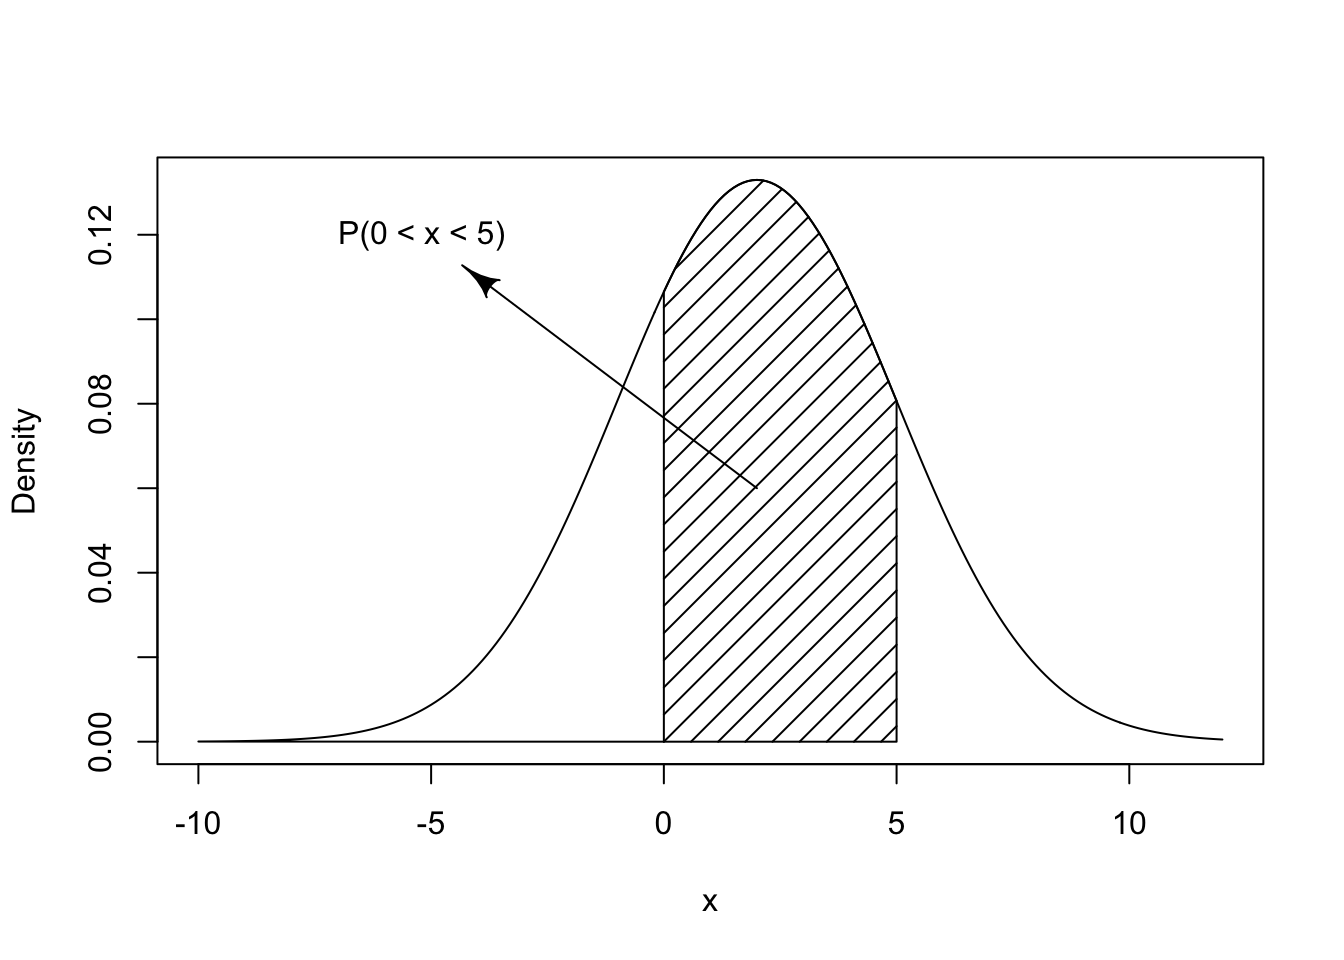
\includegraphics[width=0.6\linewidth]{statthink_files/figure-latex/Normal1-1} 

}

\caption{The Normal(2,9) Distribution}\label{fig:Normal1}
\end{figure}

The density of the Normal distribution can be computed with the aid of
the function ``\texttt{dnorm}''. The cumulative probability can be computed with
the function ``\texttt{pnorm}''. For illustrating the use of the latter function,
assume that \(X \sim \mathrm{Normal}(2,9)\). Say one is interested in the
computation of the probability \(\Prob(0 < X \leq 5)\) that the random
variable obtains a value that belongs to the interval \((0,5]\). The
required probability is indicated by the marked area in
Figure~\ref{fig:Normal1}. This area can be computed as the difference
between the probability \(\Prob(X \leq 5)\), the area to the left of 5,
and the probability \(\Prob(X \leq 0)\), the area to the left of 0:

\begin{Shaded}
\begin{Highlighting}[]
\KeywordTok{pnorm}\NormalTok{(}\DecValTok{5}\NormalTok{,}\DecValTok{2}\NormalTok{,}\DecValTok{3}\NormalTok{) }\OperatorTok{-}\StringTok{ }\KeywordTok{pnorm}\NormalTok{(}\DecValTok{0}\NormalTok{,}\DecValTok{2}\NormalTok{,}\DecValTok{3}\NormalTok{)}
\end{Highlighting}
\end{Shaded}

\begin{verbatim}
## [1] 0.58885221
\end{verbatim}

The difference is the indicated area that corresponds to the probability
of being inside the interval, which turns out to be approximately equal
to 0.589. Notice that the expectation \(\mu\) of the Normal distribution
is entered as the second argument to the function. The third argument to
the function is the standard deviation, i.e.~the square root of the
variance. In this example, the standard deviation is \(\sqrt{9}=3\).

Figure~\ref{fig:Normal2} displays the densities of the Normal
distribution for the combinations \(\mu= 0\), \(\sigma^2 = 1\) (the \emph{red}
line); \(\mu = 2\), \(\sigma^2 = 9\) (the \emph{black} line); and \(\mu = -3\),
\(\sigma^2 = 1/4\) (the \emph{green} line). Observe that the smaller the
variance the more concentrated is the distribution of the random
variable about the expectation.

\begin{figure}

{\centering 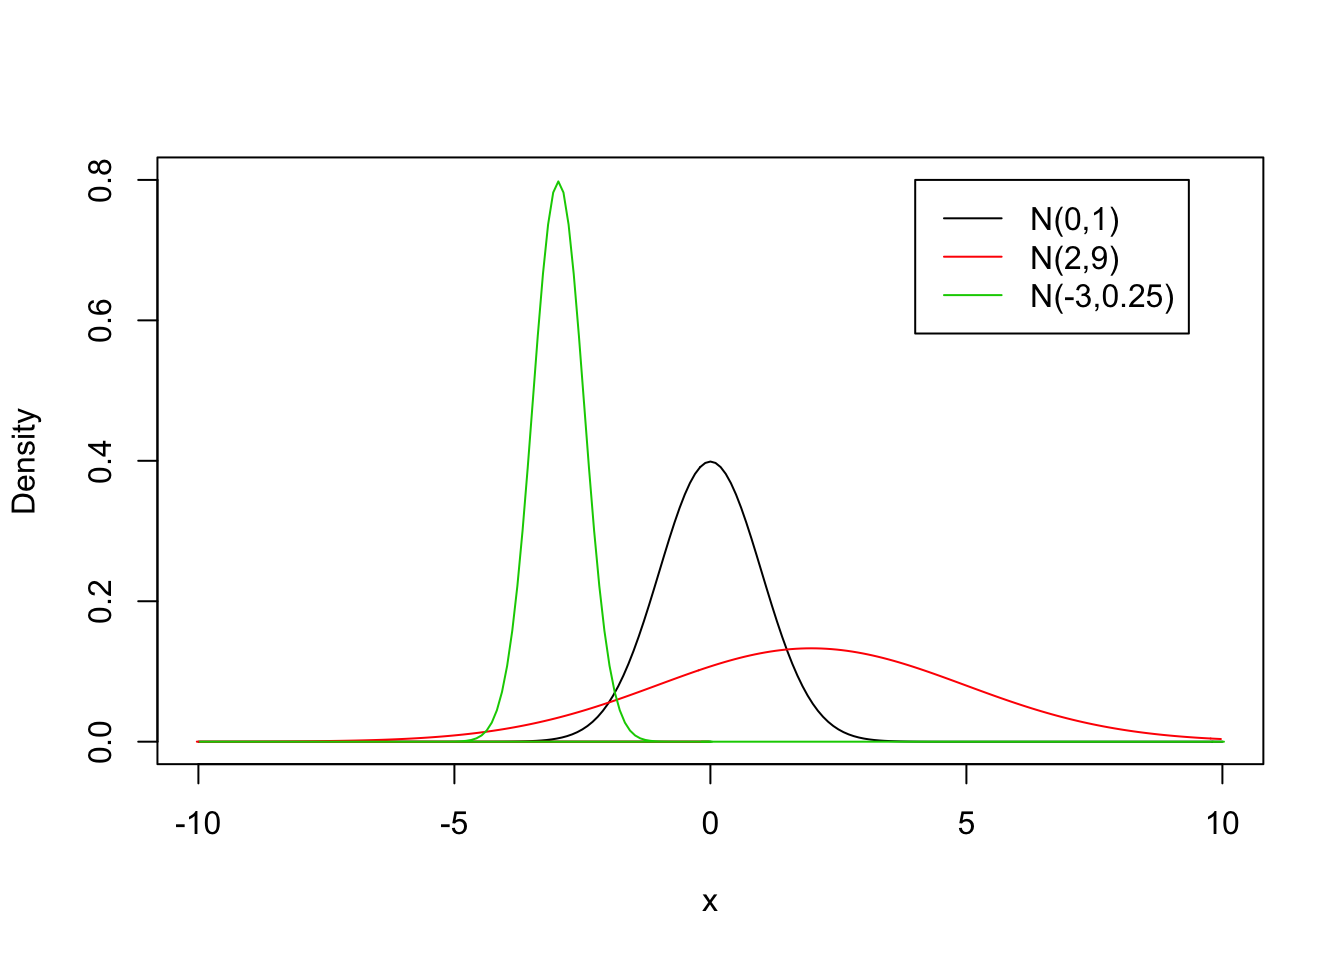
\includegraphics[width=0.6\linewidth]{statthink_files/figure-latex/Normal2-1} 

}

\caption{The Normal Distribution for Various Values of $\mu$ and $\sigma^2$}\label{fig:Normal2}
\end{figure}

\BeginKnitrBlock{example}
\protect\hypertarget{exm:exnormal1}{}{\label{exm:exnormal1} }IQ tests are a popular (and controversial) mean for
measuring intelligence. They are produced as (weighted) average of a
response to a long list of questions, designed to test different
abilities. The score of the test across the entire population is set to
be equal to 100 and the standard deviation is set to 15. The
distribution of the score is Normal. Hence, if \(X\) is the IQ score of a
random subject then \(X \sim \mathrm{Normal}(100,15^2)\).
\EndKnitrBlock{example}

\BeginKnitrBlock{example}
\protect\hypertarget{exm:exnormal2}{}{\label{exm:exnormal2} }Any measurement that is produced as a result of the
combination of many independent influencing factors is likely to poses
the Normal distribution. For example, the hight of a person is
influenced both by genetics and by the environment in which that person
grew up. Both the genetic and the environmental influences are a
combination of many factors. Thereby, it should not come as a surprise
that the heights of people in a population tend to follow the Normal
distribution.
\EndKnitrBlock{example}

\hypertarget{the-standard-normal-distribution}{%
\subsection{The Standard Normal Distribution}\label{the-standard-normal-distribution}}

The standard normal distribution is a normal distribution of
standardized values, which are called \(z\)-scores. A \(z\)-score is the
original measurement measured in units of the standard deviation from
the expectation. For example, if the expectation of a Normal
distribution is 2 and the standard deviation is \(3 = \sqrt{9}\), then the
value of 0 is 2/3 standard deviations smaller than (or to the left of)
the expectation. Hence, the \(z\)-score of the value 0 is -2/3. The
calculation of the \(z\)-score emerges from the equation:

\[(0 =)\; x = \mu + z \cdot \sigma\; (= 2 + z \cdot 3)\] The \(z\)-score
is obtained by solving the equation

\[0 = 2 + z \cdot 3 \quad \Longrightarrow \quad z = (0-2)/3 = -2/3\;.\]
In a similar way, the \(z\)-score of the value \(x = 5\) is equal to 1,
following the solution of the equation \(5 = 2 + z\cdot 3\), which leads
to \(z = (5-2)/3 = 1\).

The standard Normal distribution is the distribution of a standardized
Normal measurement. The expectation for the standard Normal distribution
is 0 and the variance is 1. When \(X \sim N(\mu,\sigma^2)\) has a Normal
distribution with expectation \(\mu\) and variance \(\sigma^2\) then the
transformed random variable \(Z = (X-\mu)/\sigma\) produces the standard
Normal distribution \(Z\sim N(0,1)\). The transformation corresponds to
the reexpression of the original measurement in terms of a new ``zero''
and a new unit of measurement. The new ``zero'' is the expectation of the
original measurement and the new unit is the standard deviation of the
original measurement.

Computation of probabilities associated with a Normal random variable
\(X\) can be carried out with the aid of the standard Normal distribution.
For example, consider the computation of the probability
\(\Prob(0 < X \leq 5)\) for \(X \sim N(2, 9)\), that has expectation \(\mu=2\)
and standard deviation \(\sigma = 3\). Consider \(X\)'s standardized values:
\(Z = (X-2)/3\). The boundaries of the interval \([0,5]\), namely \(0\) and
\(5\), have standardized \(z\)-scores of \((0-2)/3=-2/3\) and \((5-2)/3 =1\),
respectively. Clearly, the original measurement \(X\) falls between the
original boundaries (\(0 < X \leq 5\)) if, and only if, the standardized
measurement \(Z\) falls between the standardized boundaries
(\(-2/3 < Z \leq 1\)). Therefore, the probability that \(X\) obtains a value
in the range \([0,5]\) is equal to the probability that \(Z\) obtains a
value in the range \([-2/3,1]\).

\begin{figure}

{\centering 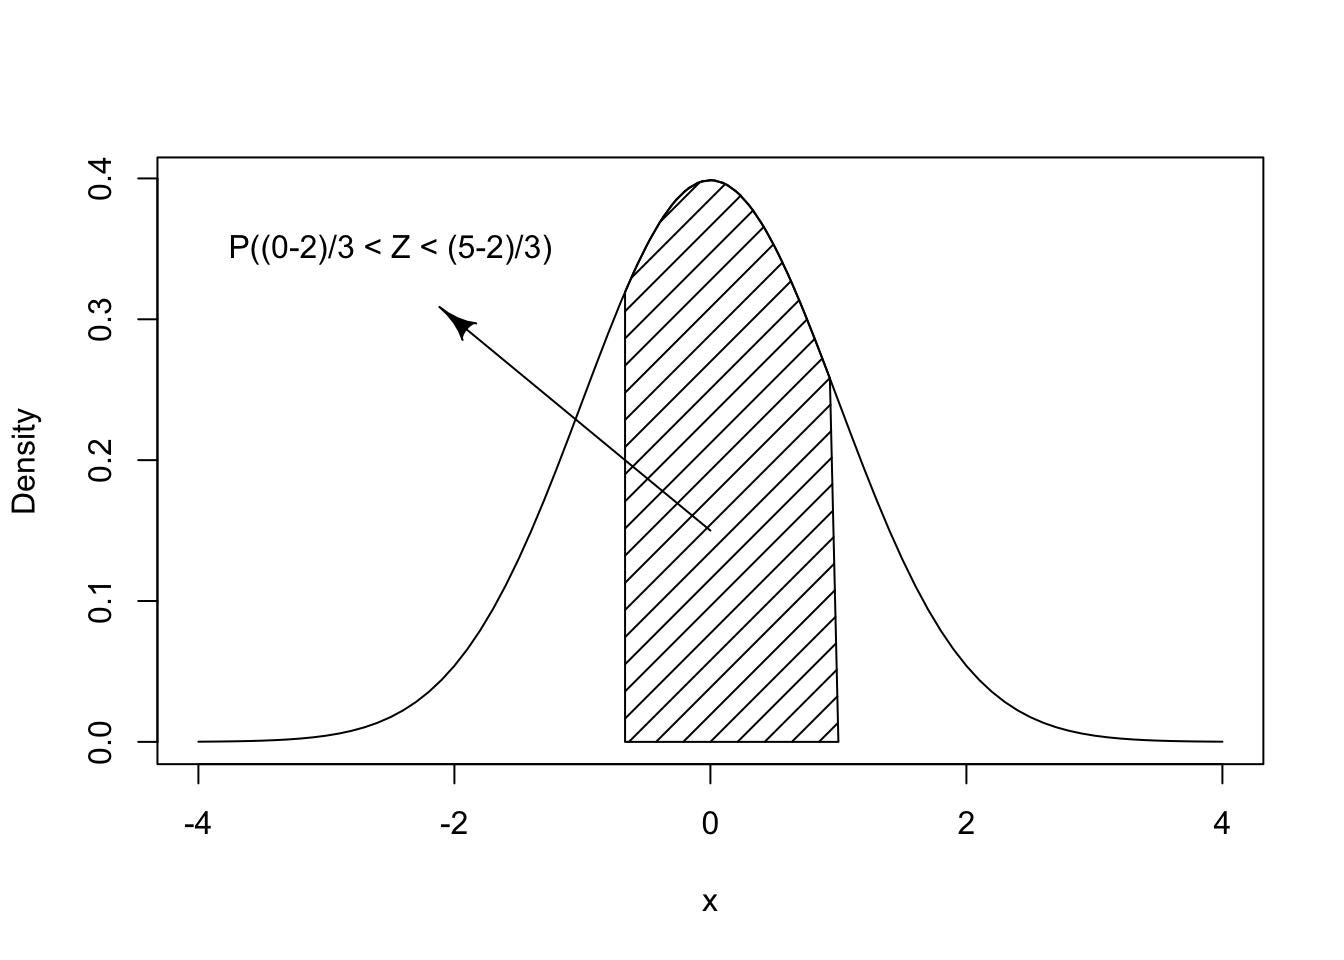
\includegraphics[width=0.6\linewidth]{statthink_files/figure-latex/Normal3-1} 

}

\caption{The Standard Normal Distribution}\label{fig:Normal3}
\end{figure}

The function ``\texttt{pnorm}'' was used in the previous subsection in order to
compute that probability that \(X\) obtains values between 0 and 5. The
computation produced the probability 0.5888522. We can repeat the
computation by the application of the same function to the standardized
values:

\begin{Shaded}
\begin{Highlighting}[]
\KeywordTok{pnorm}\NormalTok{((}\DecValTok{5-2}\NormalTok{)}\OperatorTok{/}\DecValTok{3}\NormalTok{) }\OperatorTok{-}\StringTok{ }\KeywordTok{pnorm}\NormalTok{((}\DecValTok{0-2}\NormalTok{)}\OperatorTok{/}\DecValTok{3}\NormalTok{)}
\end{Highlighting}
\end{Shaded}

\begin{verbatim}
## [1] 0.58885221
\end{verbatim}

The value that is being computed, the area under the graph for the
standard Normal distribution, is presented in Figure~\ref{fig:Normal3}.
Recall that 3 arguments where specified in the previous application of
the function ``\texttt{pnorm}'': the \(x\) value, the expectation, and the standard
deviation. In the given application we did not specify the last two
arguments, only the first one. (Notice that the output of the expression
``\texttt{(5-2)/3}'' is a single number and, likewise, the output of the
expression ``\texttt{(0-2)/3}'' is also a single number.)

Most \texttt{R} function have many arguments that enables flexible application
in a wide range of settings. For convenience, however, default values
are set to most of these arguments. These default values are used unless
an alternative value for the argument is set when the function is
called. The default value of the second argument of the function
``\texttt{pnorm}'' that specifies the expectation is ``\texttt{mean=0}'', and the default
value of the third argument that specifies the standard deviation is
``\texttt{sd=1}''. Therefore, if no other value is set for these arguments the
function computes the cumulative distribution function of the standard
Normal distribution.

\hypertarget{computing-percentiles}{%
\subsection{Computing Percentiles}\label{computing-percentiles}}

Consider the issue of determining the range that contains 95\% of the
probability for a Normal random variable. We start with the standard
Normal distribution. Consult Figure~\ref{fig:Normal4}. The figure
displays the standard Normal distribution with the central region
shaded. The area of the shaded region is 0.95.

We may find the \(z\)-values of the boundaries of the region, denoted in
the figure as \(z_0\) and \(z_1\) by the investigation of the cumulative
distribution function. Indeed, in order to have 95\% of the distribution
in the central region one should leave out 2.5\% of the distribution in
each of the two tails. That is, 0.025 should be the area of the unshaded
region to the right of \(z_1\) and, likewise, 0.025 should be the area of
the unshaded region to the left of \(z_0\). In other words, the cumulative
probability up to \(z_0\) should be 0.025 and the cumulative distribution
up to \(z_1\) should be 0.975.

In general, given a random variable \(X\) and given a percent \(p\), the \(x\)
value with the property that the cumulative distribution up to \(x\) is
equal to the probability \(p\) is called the \(p\)-\emph{percentile} of the
distribution. Here we seek the 2.5\%-percentile and the 97.5\%-percentile
of the standard Normal distribution.

\begin{figure}

{\centering 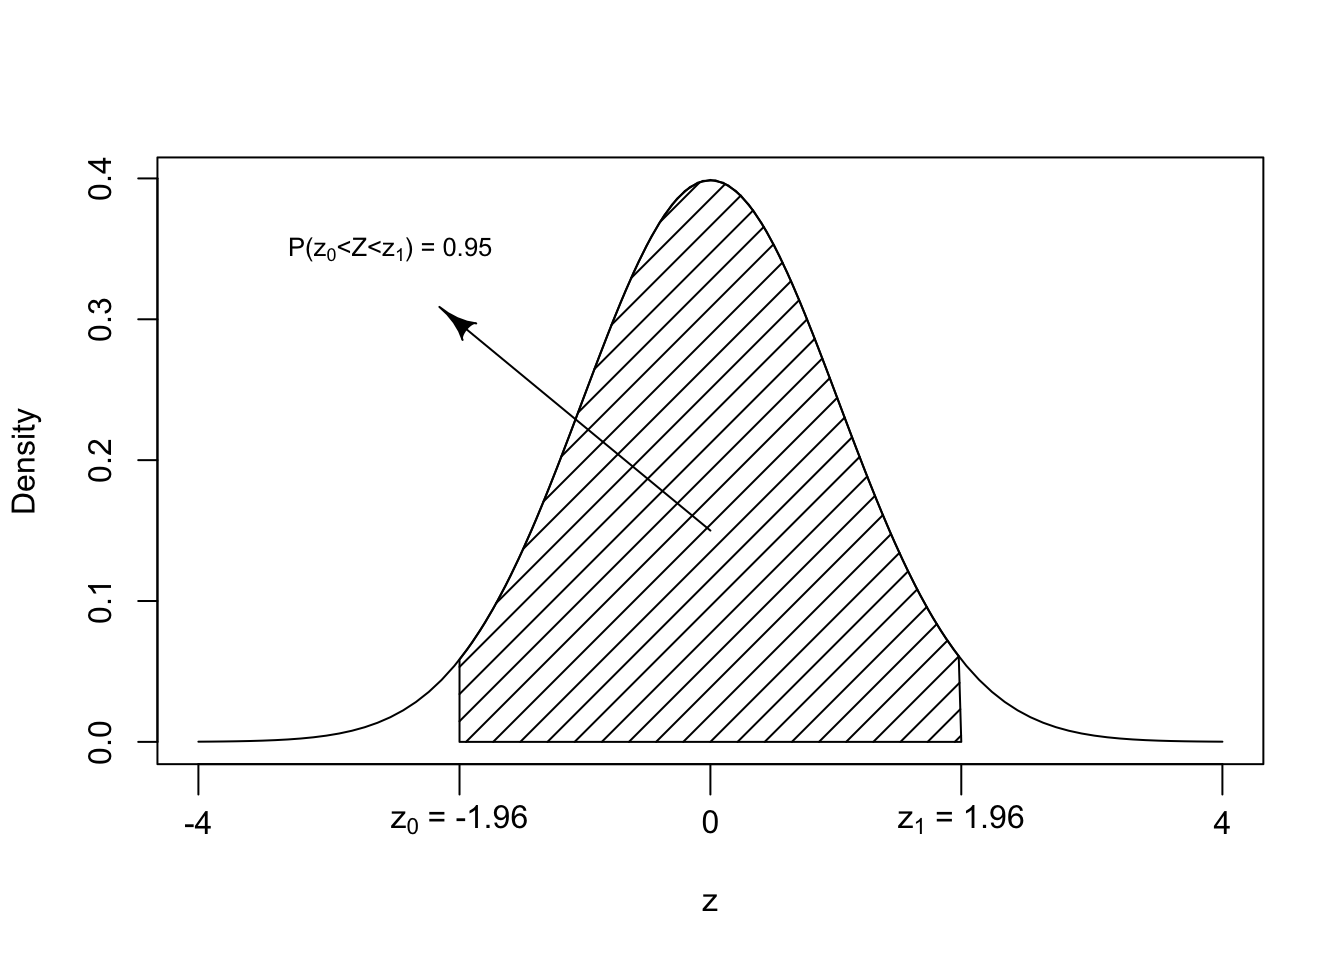
\includegraphics[width=0.6\linewidth]{statthink_files/figure-latex/Normal4-1} 

}

\caption{Central 95$\%$ of the Standard Normal Distribution}\label{fig:Normal4}
\end{figure}

The percentiles of the Normal distribution are computed by the function
``\texttt{qnorm}''. The first argument to the function is a probability (or a
sequence of probabilities), the second and third arguments are the
expectation and the standard deviations of the normal distribution. The
default values to these arguments are set to 0 and 1, respectively.
Hence if these arguments are not provided the function computes the
percentiles of the standard Normal distribution. Let us apply the
function in order to compute \(z_1\) and \(z_0\):

\begin{Shaded}
\begin{Highlighting}[]
\KeywordTok{qnorm}\NormalTok{(}\FloatTok{0.975}\NormalTok{)}
\end{Highlighting}
\end{Shaded}

\begin{verbatim}
## [1] 1.959964
\end{verbatim}

\begin{Shaded}
\begin{Highlighting}[]
\KeywordTok{qnorm}\NormalTok{(}\FloatTok{0.025}\NormalTok{)}
\end{Highlighting}
\end{Shaded}

\begin{verbatim}
## [1] -1.959964
\end{verbatim}

Observe that \(z_1\) is practically equal to 1.96 and
\(z_0 = -1.96 = -z_1\). The fact that \(z_0\) is the negative of \(z_1\)
results from the symmetry of the standard Normal distribution about 0.
As a conclusion we get that for the standard Normal distribution 95\% of
the probability is concentrated in the range \([-1.96, 1.96]\).

\begin{figure}

{\centering 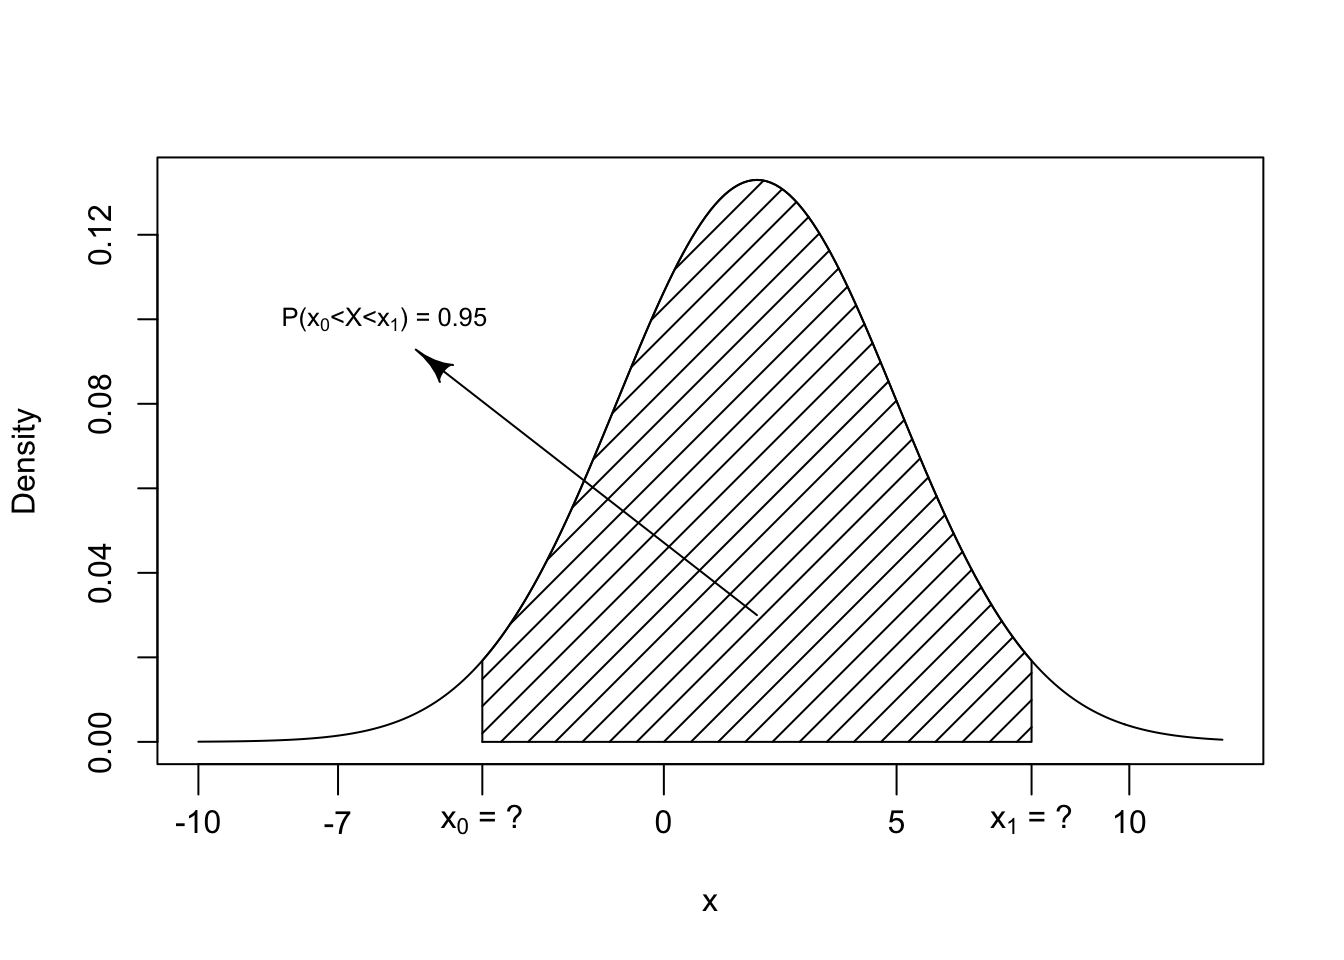
\includegraphics[width=0.6\linewidth]{statthink_files/figure-latex/Normal5-1} 

}

\caption{Central 95$\%$ of the Normal(2,9) Distribution}\label{fig:Normal5}
\end{figure}

The problem of determining the central range that contains 95\% of the
distribution can be addresses in the context of the original measurement
\(X\) (See Figure~\ref{fig:Normal5}). We seek in this case an interval
centered at the expectation 2, which is the center of the distribution
of \(X\), unlike 0 which was the center of the standardized values \(Z\).
One way of solving the problem is via the application of the function
``\texttt{qnorm}'' with the appropriate values for the expectation and the
standard deviation:

\begin{Shaded}
\begin{Highlighting}[]
\KeywordTok{qnorm}\NormalTok{(}\FloatTok{0.975}\NormalTok{,}\DecValTok{2}\NormalTok{,}\DecValTok{3}\NormalTok{)}
\end{Highlighting}
\end{Shaded}

\begin{verbatim}
## [1] 7.879892
\end{verbatim}

\begin{Shaded}
\begin{Highlighting}[]
\KeywordTok{qnorm}\NormalTok{(}\FloatTok{0.025}\NormalTok{,}\DecValTok{2}\NormalTok{,}\DecValTok{3}\NormalTok{)}
\end{Highlighting}
\end{Shaded}

\begin{verbatim}
## [1] -3.879892
\end{verbatim}

Hence, we get that \(x_0 = -3.88\) has the property that the total
probability to its left is 0.025 and \(x_1 = 7.88\) has the property that
the total probability to its right is 0.025. The total probability in
the range \([-3.88, 7.88]\) is 0.95.

An alternative approach for obtaining the given interval exploits the
interval that was obtained for the standardized values. An interval
\([-1.96,1.96]\) of standardized \(z\)-values corresponds to an interval
\([2 - 1.96 \cdot 3, 2 + 1.96\cdot 3]\) of the original \(x\)-values:

\begin{Shaded}
\begin{Highlighting}[]
\DecValTok{2} \OperatorTok{+}\StringTok{ }\KeywordTok{qnorm}\NormalTok{(}\FloatTok{0.975}\NormalTok{)}\OperatorTok{*}\DecValTok{3}
\end{Highlighting}
\end{Shaded}

\begin{verbatim}
## [1] 7.879892
\end{verbatim}

\begin{Shaded}
\begin{Highlighting}[]
\DecValTok{2} \OperatorTok{+}\StringTok{ }\KeywordTok{qnorm}\NormalTok{(}\FloatTok{0.025}\NormalTok{)}\OperatorTok{*}\DecValTok{3}
\end{Highlighting}
\end{Shaded}

\begin{verbatim}
## [1] -3.879892
\end{verbatim}

Hence, we again produce the interval \([-3.88,7.88]\), the interval that
was obtained before as the central interval that contains 95\% of the
distribution of the \(\mathrm{Normal}(2,9)\) random variable.

In general, if \(X \sim N(\mu,\sigma)\) is a Normal random variable then
the interval \([\mu - 1.96 \cdot \sigma, \mu + 1.96 \cdot \sigma]\)
contains 95\% of the distribution of the random variable. Frequently one
uses the notation \(\mu \pm 1.96 \cdot \sigma\) to describe such an
interval.

\hypertarget{outliers-and-the-normal-distribution}{%
\subsection{Outliers and the Normal Distribution}\label{outliers-and-the-normal-distribution}}

Consider, next, the computation of the interquartile range in the Normal
distribution. Recall that the interquartile range is the length of the
central interval that contains 50\% of the distribution. This interval
starts at the first quartile (Q1), the value that splits the
distribution so that 25\% of the distribution is to the left of the value
and 75\% is to the right of it. The interval ends at the third quartile
(Q3) where 75\% of the distribution is to the left and 25\% is to the
right.

For the standard Normal the third and first quartiles can be computed
with the aid of the function ``\texttt{qnorm}'':

\begin{Shaded}
\begin{Highlighting}[]
\KeywordTok{qnorm}\NormalTok{(}\FloatTok{0.75}\NormalTok{)}
\end{Highlighting}
\end{Shaded}

\begin{verbatim}
## [1] 0.67448975
\end{verbatim}

\begin{Shaded}
\begin{Highlighting}[]
\KeywordTok{qnorm}\NormalTok{(}\FloatTok{0.25}\NormalTok{)}
\end{Highlighting}
\end{Shaded}

\begin{verbatim}
## [1] -0.67448975
\end{verbatim}

Observe that for the standard Normal distribution one has that 75\% of
the distribution is to the left of the value 0.6744898, which is the
third quartile of this distribution. Likewise, 25\% of the standard
Normal distribution are to the left of the value -0.6744898, which is
the first quartile. the interquartile range is the length of the
interval between the third and the first quartiles. In the case of the
standard Normal distribution this length is equal to
\(0.6744898 - (-0.6744898) = 1.348980\).

In Chapter~\ref{ChapDescriptiveStat} we considered box plots as a mean for
the graphical display of numerical data. The box plot includes a
vertical rectangle that initiates at the first quartile and ends at the
third quartile, with the median marked within the box. The rectangle
contains 50\% of the data. Whiskers extends from the ends of this
rectangle to the smallest and to the largest data values that are not
outliers. Outliers are values that lie outside of the normal range of
the data. Outliers are identified as values that are more then 1.5 times
the interquartile range away from the ends of the central rectangle.
Hence, a value is an outlier if it is larger than the third quartile
plus 1.5 times the interquartile range or if it is less than the first
quartile minus 1.5 times the interquartile range.

How likely is it to obtain an outlier value when the measurement has the
standard Normal distribution? We obtained that the third quartile of the
standard Normal distribution is equal to 0.6744898 and the first
quartile is minus this value. The interquartile range is the difference
between the third and first quartiles. The upper and lower thresholds
for the defining outliers are:

\begin{Shaded}
\begin{Highlighting}[]
\KeywordTok{qnorm}\NormalTok{(}\FloatTok{0.75}\NormalTok{) }\OperatorTok{+}\StringTok{ }\FloatTok{1.5}\OperatorTok{*}\NormalTok{(}\KeywordTok{qnorm}\NormalTok{(}\FloatTok{0.75}\NormalTok{)}\OperatorTok{-}\KeywordTok{qnorm}\NormalTok{(}\FloatTok{0.25}\NormalTok{))}
\end{Highlighting}
\end{Shaded}

\begin{verbatim}
## [1] 2.697959
\end{verbatim}

\begin{Shaded}
\begin{Highlighting}[]
\KeywordTok{qnorm}\NormalTok{(}\FloatTok{0.25}\NormalTok{) }\OperatorTok{-}\StringTok{ }\FloatTok{1.5}\OperatorTok{*}\NormalTok{(}\KeywordTok{qnorm}\NormalTok{(}\FloatTok{0.75}\NormalTok{)}\OperatorTok{-}\KeywordTok{qnorm}\NormalTok{(}\FloatTok{0.25}\NormalTok{))}
\end{Highlighting}
\end{Shaded}

\begin{verbatim}
## [1] -2.697959
\end{verbatim}

Hence, a value larger than 2.697959 or smaller than -2.697959 would be
identified as an outlier.

The probability of being less than the upper threshold 2.697959 in the
standard Normal distribution is computed with the expression
``\texttt{pnorm(2.697959)}''. The probability of being above the threshold is 1
minus that probability, which is the outcome of the expression
``\texttt{1-pnorm(2.697959)}''.

By the symmetry of the standard Normal distribution we get that the
probability of being below the lower threshold -2.697959 is equal to the
probability of being above the upper threshold. Consequently, the
probability of obtaining an outlier is equal to twice the probability of
being above the upper threshold:

\begin{Shaded}
\begin{Highlighting}[]
\DecValTok{2}\OperatorTok{*}\NormalTok{(}\DecValTok{1}\OperatorTok{-}\KeywordTok{pnorm}\NormalTok{(}\FloatTok{2.697959}\NormalTok{))}
\end{Highlighting}
\end{Shaded}

\begin{verbatim}
## [1] 0.0069766033
\end{verbatim}

We get that for the standard Normal distribution the probability of an
outlier is approximately 0.7\%.

\hypertarget{approximation-of-the-binomial-distribution}{%
\section{Approximation of the Binomial Distribution}\label{approximation-of-the-binomial-distribution}}

The Normal distribution emerges frequently as an approximation of the
distribution of data characteristics. The probability theory that
mathematically establishes such approximation is called the Central
Limit Theorem and is the subject of the next chapter. In this section we
demonstrate the Normal approximation in the context of the Binomial
distribution.

\hypertarget{approximate-binomial-probabilities-and-percentiles}{%
\subsection{Approximate Binomial Probabilities and Percentiles}\label{approximate-binomial-probabilities-and-percentiles}}

Consider, for example, the probability of obtaining between 1940 and
2060 heads when tossing 4,000 fair coins. Let \(X\) be the total number of
heads. The tossing of a coin is a trial with two possible outcomes:
``Head'' and ``Tail.'' The probability of a ``Head'' is 0.5 and there are
4,000 trials. Let us call obtaining a ``Head'' in a trial a ``Success''.
Observe that the random variable \(X\) counts the total number of
successes. Hence, \(X \sim \mathrm{Binomial}(4000,0.5)\).

The probability \(\Prob(1940 \leq X \leq 2060)\) can be computed as the
difference between the probability \(\Prob(X \leq 2060)\) of being less or
equal to 2060 and the probability \(\Prob(X < 1940)\) of being strictly
less than 1940. However, 1939 is the largest integer that is still
strictly less than the integer 1940. As a result we get that
\(\Prob(X < 1940) = \Prob(X \leq 1939)\). Consequently,
\(\Prob(1940 \leq X \leq 2060) = \Prob(X \leq 2060) - \Prob(X \leq 1939)\).

Applying the function ``\texttt{pbinom}'' for the computation of the Binomial
cumulative probability, namely the probability of being less or equal to
a given value, we get that the probability in the range between 1940 and
2060 is equal to

\begin{Shaded}
\begin{Highlighting}[]
\KeywordTok{pbinom}\NormalTok{(}\DecValTok{2060}\NormalTok{,}\DecValTok{4000}\NormalTok{,}\FloatTok{0.5}\NormalTok{) }\OperatorTok{-}\StringTok{ }\KeywordTok{pbinom}\NormalTok{(}\DecValTok{1939}\NormalTok{,}\DecValTok{4000}\NormalTok{,}\FloatTok{0.5}\NormalTok{)}
\end{Highlighting}
\end{Shaded}

\begin{verbatim}
## [1] 0.9442883
\end{verbatim}

This is an exact computation. The Normal approximation produces an
approximate evaluation, not an exact computation. The Normal
approximation replaces Binomial computations by computations carried out
for the Normal distribution. The computation of a probability for a
Binomial random variable is replaced by computation of probability for a
Normal random variable that has the same expectation and standard
deviation as the Binomial random variable.

Notice that if \(X \sim \mathrm{Binomial}(4000,0.5)\) then the expectation
is \(\Expec(X) = 4,000 \times 0.5 = 2,000\) and the variance is
\(\Var(X) = 4,000 \times 0.5 \times 0.5 = 1,000\), with the standard
deviation being the square root of the variance. Repeating the same
computation that we conducted for the Binomial random variable, but this
time with the function ``\texttt{pnorm}'' that is used for the computation of the
Normal cumulative probability, we get:

\begin{Shaded}
\begin{Highlighting}[]
\NormalTok{mu <-}\StringTok{ }\DecValTok{4000}\OperatorTok{*}\FloatTok{0.5}
\NormalTok{sig <-}\StringTok{ }\KeywordTok{sqrt}\NormalTok{(}\DecValTok{4000}\OperatorTok{*}\FloatTok{0.5}\OperatorTok{*}\FloatTok{0.5}\NormalTok{)}
\KeywordTok{pnorm}\NormalTok{(}\DecValTok{2060}\NormalTok{,mu,sig) }\OperatorTok{-}\StringTok{ }\KeywordTok{pnorm}\NormalTok{(}\DecValTok{1939}\NormalTok{,mu,sig)}
\end{Highlighting}
\end{Shaded}

\begin{verbatim}
## [1] 0.94424412
\end{verbatim}

Observe that in this example the Normal approximation of the probability
(0.9442441) agrees with the Binomial computation of the probability
(0.9442883) up to 3 significant digits.

Normal computations may also be applied in order to find approximate
percentiles of the Binomial distribution. For example, let us identify
the central region that contains for a \(\mathrm{Binomial}(4000,0.5)\)
random variable (approximately) 95\% of the distribution. Towards that
end we can identify the boundaries of the region for the Normal
distribution with the same expectation and standard deviation as that of
the target Binomial distribution:

\begin{Shaded}
\begin{Highlighting}[]
\KeywordTok{qnorm}\NormalTok{(}\FloatTok{0.975}\NormalTok{,mu,sig)}
\end{Highlighting}
\end{Shaded}

\begin{verbatim}
## [1] 2061.9795
\end{verbatim}

\begin{Shaded}
\begin{Highlighting}[]
\KeywordTok{qnorm}\NormalTok{(}\FloatTok{0.025}\NormalTok{,mu,sig)}
\end{Highlighting}
\end{Shaded}

\begin{verbatim}
## [1] 1938.0205
\end{verbatim}

After rounding to the nearest integer we get the interval \([1938,2062]\)
as a proposed central region.

In order to validate the proposed region we may repeat the computation
under the actual Binomial distribution:

\begin{Shaded}
\begin{Highlighting}[]
\KeywordTok{qbinom}\NormalTok{(}\FloatTok{0.975}\NormalTok{,}\DecValTok{4000}\NormalTok{,}\FloatTok{0.5}\NormalTok{)}
\end{Highlighting}
\end{Shaded}

\begin{verbatim}
## [1] 2062
\end{verbatim}

\begin{Shaded}
\begin{Highlighting}[]
\KeywordTok{qbinom}\NormalTok{(}\FloatTok{0.025}\NormalTok{,}\DecValTok{4000}\NormalTok{,}\FloatTok{0.5}\NormalTok{)}
\end{Highlighting}
\end{Shaded}

\begin{verbatim}
## [1] 1938
\end{verbatim}

Again, we get the interval \([1938,2062]\) as the central region, in
agreement with the one proposed by the Normal approximation. Notice that
the function ``\texttt{qbinom}'' produces the percentiles of the Binomial
distribution. It may not come as a surprise to learn that ``\texttt{qpois}'',
``\texttt{qunif}'', ``\texttt{qexp}'' compute the percentiles of the Poisson, Uniform and
Exponential distributions, respectively.

The ability to approximate one distribution by the other, when
computation tools for both distributions are handy, seems to be of
questionable importance. Indeed, the significance of the Normal
approximation is not so much in its ability to approximate the Binomial
distribution as such. Rather, the important point is that the Normal
distribution may serve as an approximation to a wide class of
distributions, with the Binomial distribution being only one example.
Computations that are based on the Normal approximation will be valid
for all members in the class of distributions, including cases where we
don't have the computational tools at our disposal or even in cases
where we do not know what the exact distribution of the member is! As
promised, a more detailed discussion of the Normal approximation in a
wider context will be presented in the next chapter.

On the other hand, one need not assume that any distribution is well
approximated by the Normal distribution. For example, the distribution
of wealth in the population tends to be skewed, with more than 50\% of
the people possessing less than 50\% of the wealth and small percentage
of the people possessing the majority of the wealth. The Normal
distribution is not a good model for such distribution. The Exponential
distribution, or distributions similar to it, may be more appropriate.

\hypertarget{continuity-corrections}{%
\subsection{Continuity Corrections}\label{continuity-corrections}}

In order to complete this section let us look more carefully at the
Normal approximations of the Binomial distribution.

\begin{figure}

{\centering 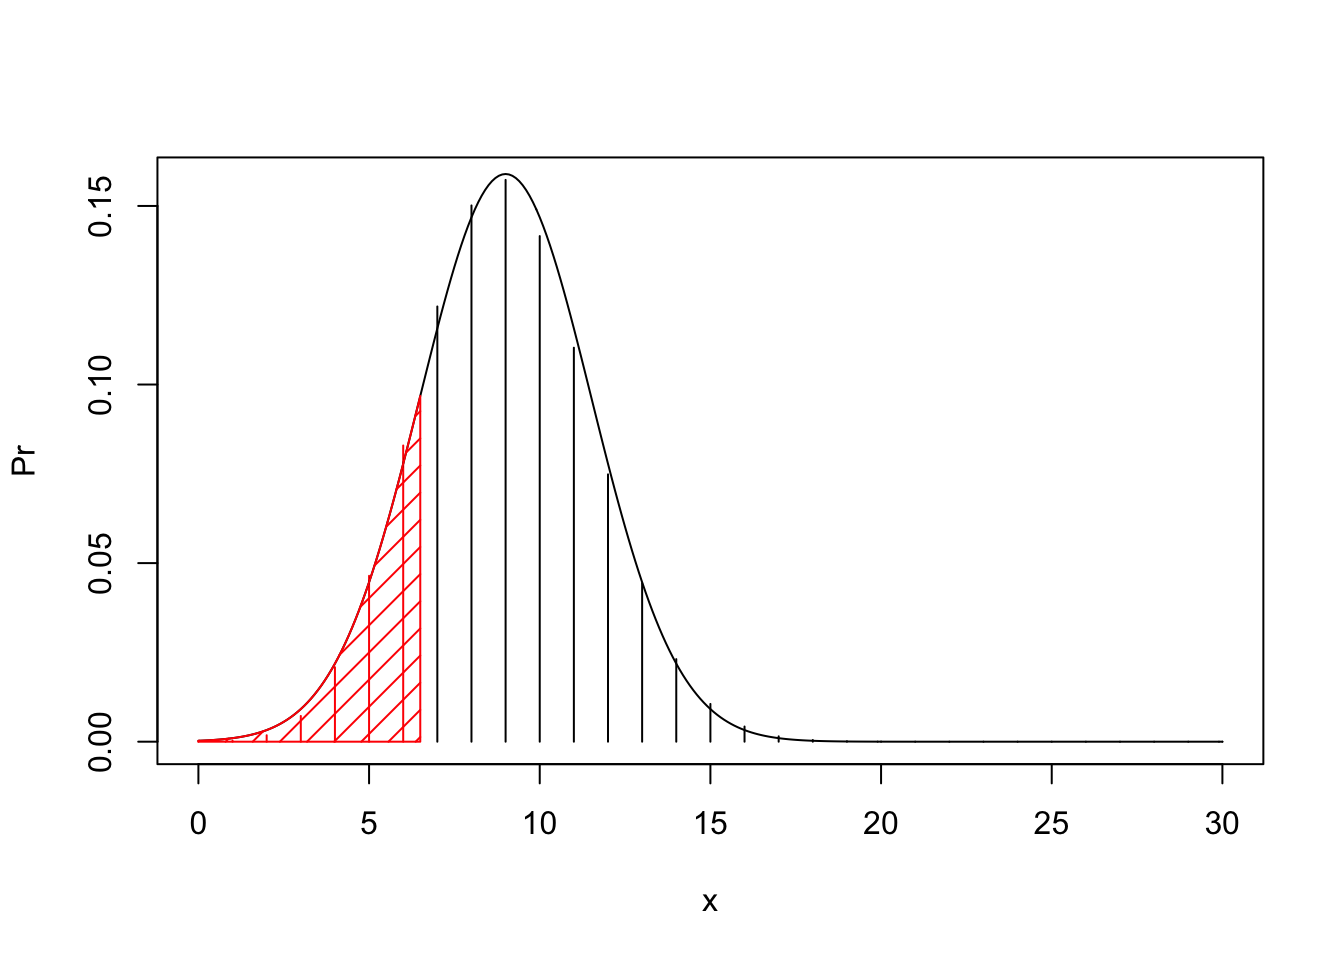
\includegraphics[width=0.6\linewidth]{statthink_files/figure-latex/Normal6-1} 

}

\caption{Normal Approximation of the Binomial Distribution}\label{fig:Normal6}
\end{figure}

In principle, the Normal approximation is valid when \(n\), the number of
independent trials in the Binomial distribution, is large. When \(n\) is
relatively small the approximation may not be so good. Indeed, take
\(X \sim \mathrm{Binomial}(30,0.3)\) and consider the probability
\(\Prob(X \leq 6)\). Compare the actual probability to the Normal
approximation:

\begin{Shaded}
\begin{Highlighting}[]
\KeywordTok{pbinom}\NormalTok{(}\DecValTok{6}\NormalTok{,}\DecValTok{30}\NormalTok{,}\FloatTok{0.3}\NormalTok{)}
\end{Highlighting}
\end{Shaded}

\begin{verbatim}
## [1] 0.15952298
\end{verbatim}

\begin{Shaded}
\begin{Highlighting}[]
\KeywordTok{pnorm}\NormalTok{(}\DecValTok{6}\NormalTok{,}\DecValTok{30}\OperatorTok{*}\FloatTok{0.3}\NormalTok{,}\KeywordTok{sqrt}\NormalTok{(}\DecValTok{30}\OperatorTok{*}\FloatTok{0.3}\OperatorTok{*}\FloatTok{0.7}\NormalTok{))}
\end{Highlighting}
\end{Shaded}

\begin{verbatim}
## [1] 0.11599886
\end{verbatim}

The Normal approximation, which is equal to 0.1159989, is not too close
to the actual probability, which is equal to 0.1595230.

A naïve application of the Normal approximation for the
\(\mathrm{Binomial}(n,p)\) distribution may not be so good when the number
of trials \(n\) is small. Yet, a small modification of the approximation
may produce much better results. In order to explain the modification
consult Figure~\ref{fig:Normal6} where you will find the bar plot of the
Binomial distribution with the density of the approximating Normal
distribution superimposed on top of it. The target probability is the
sum of heights of the bars that are painted in \emph{red}. In the naïve
application of the Normal approximation we used the area under the
normal density which is to the left of the bar associated with the value
\(x=6\).

Alternatively, you may associate with each bar located at \(x\) the area
under the normal density over the interval \([x-0.5, x+0.5]\). The
resulting correction to the approximation will use the Normal
probability of the event \(\{X \leq 6.5\}\), which is the area shaded in
\emph{red}. The application of this approximation, which is called
\emph{continuity correction} produces:

\begin{Shaded}
\begin{Highlighting}[]
\KeywordTok{pnorm}\NormalTok{(}\FloatTok{6.5}\NormalTok{,}\DecValTok{30}\OperatorTok{*}\FloatTok{0.3}\NormalTok{,}\KeywordTok{sqrt}\NormalTok{(}\DecValTok{30}\OperatorTok{*}\FloatTok{0.3}\OperatorTok{*}\FloatTok{0.7}\NormalTok{))}
\end{Highlighting}
\end{Shaded}

\begin{verbatim}
## [1] 0.15961928
\end{verbatim}

Observe that the corrected approximation is much closer to the target
probability, which is 0.1595230, and is substantially better that the
uncorrected approximation which was 0.1159989. Generally, it is
recommended to apply the continuity correction to the Normal
approximation of a discrete distribution.

Consider the \(\mathrm{Binomial}(n,p)\) distribution. Another situation
where the Normal approximation may fail is when \(p\), the probability of
``Success'' in the Binomial distribution, is too close to 0 (or too close
to 1). Recall, that for large \(n\) the Poisson distribution emerged as an
approximation of the Binomial distribution in such a setting. One may
expect that when \(n\) is large and \(p\) is small then the Poisson
distribution may produce a better approximation of a Binomial
probability. When the Poisson distribution is used for the approximation
we call it a \emph{Poisson Approximation}.

Let us consider an example. Let us analyze 3 Binomial distributions. The
expectation in all the distributions is equal to 2 but the number of
trials, \(n\), vary. In the first case \(n=20\) (and hence \(p=0.1\)), in the
second \(n=200\) (and \(p=0.01\)), and in the third \(n=2,000\) (and
\(p=0.001\). In all three cases we will be interested in the probability
of obtaining a value less or equal to 3.

The Poisson approximation replaces computations conducted under the
Binomial distribution with Poisson computations, with a Poisson
distribution that has the same expectation as the Binomial. Since in all
three cases the expectation is equal to 2 we get that the same Poisson
approximation is used to the three probabilities:

\begin{Shaded}
\begin{Highlighting}[]
\KeywordTok{ppois}\NormalTok{(}\DecValTok{3}\NormalTok{,}\DecValTok{2}\NormalTok{)}
\end{Highlighting}
\end{Shaded}

\begin{verbatim}
## [1] 0.85712346
\end{verbatim}

The actual Binomial probability in the first case (\(n=20\), \(p=0.1\)) and
a Normal approximation thereof are:

\begin{Shaded}
\begin{Highlighting}[]
\KeywordTok{pbinom}\NormalTok{(}\DecValTok{3}\NormalTok{,}\DecValTok{20}\NormalTok{,}\FloatTok{0.1}\NormalTok{)}
\end{Highlighting}
\end{Shaded}

\begin{verbatim}
## [1] 0.86704668
\end{verbatim}

\begin{Shaded}
\begin{Highlighting}[]
\KeywordTok{pnorm}\NormalTok{(}\FloatTok{3.5}\NormalTok{,}\DecValTok{2}\NormalTok{,}\KeywordTok{sqrt}\NormalTok{(}\DecValTok{20}\OperatorTok{*}\FloatTok{0.1}\OperatorTok{*}\FloatTok{0.9}\NormalTok{))}
\end{Highlighting}
\end{Shaded}

\begin{verbatim}
## [1] 0.86822376
\end{verbatim}

Observe that the Normal approximation (with a continuity correction) is
better than the Poisson approximation in this case.

In the second case (\(n=200\), \(p=0.01\)) the actual Binomial probability
and the Normal approximation of the probability are:

\begin{Shaded}
\begin{Highlighting}[]
\KeywordTok{pbinom}\NormalTok{(}\DecValTok{3}\NormalTok{,}\DecValTok{200}\NormalTok{,}\FloatTok{0.01}\NormalTok{)}
\end{Highlighting}
\end{Shaded}

\begin{verbatim}
## [1] 0.85803403
\end{verbatim}

\begin{Shaded}
\begin{Highlighting}[]
\KeywordTok{pnorm}\NormalTok{(}\FloatTok{3.5}\NormalTok{,}\DecValTok{2}\NormalTok{,}\KeywordTok{sqrt}\NormalTok{(}\DecValTok{200}\OperatorTok{*}\FloatTok{0.01}\OperatorTok{*}\FloatTok{0.99}\NormalTok{))}
\end{Highlighting}
\end{Shaded}

\begin{verbatim}
## [1] 0.85678899
\end{verbatim}

Observe that the Poisson approximation that produces 0.8571235 is
slightly closer to the target than the Normal approximation. The greater
accuracy of the Poisson approximation for the case where \(n\) is large
and \(p\) is small is more pronounced in the final case (\(n=2000\),
\(p=0.001\)) where the target probability and the Normal approximation
are:

\begin{Shaded}
\begin{Highlighting}[]
\KeywordTok{pbinom}\NormalTok{(}\DecValTok{3}\NormalTok{,}\DecValTok{2000}\NormalTok{,}\FloatTok{0.001}\NormalTok{)}
\end{Highlighting}
\end{Shaded}

\begin{verbatim}
## [1] 0.85721377
\end{verbatim}

\begin{Shaded}
\begin{Highlighting}[]
\KeywordTok{pnorm}\NormalTok{(}\FloatTok{3.5}\NormalTok{,}\DecValTok{2}\NormalTok{,}\KeywordTok{sqrt}\NormalTok{(}\DecValTok{2000}\OperatorTok{*}\FloatTok{0.001}\OperatorTok{*}\FloatTok{0.999}\NormalTok{))}
\end{Highlighting}
\end{Shaded}

\begin{verbatim}
## [1] 0.85569842
\end{verbatim}

Compare the actual Binomial probability, which is equal to 0.8572138, to
the Poisson approximation that produced 0.8571235. The Normal
approximation, 0.8556984, is slightly off, but is still acceptable.

\hypertarget{Normal4}{%
\section{Exercises}\label{Normal4}}

\BeginKnitrBlock{exercise}
\protect\hypertarget{exr:unnamed-chunk-89}{}{\label{exr:unnamed-chunk-89} }Consider the problem of establishing regulations
concerning the maximum number of people who can occupy a lift. In
particular, we would like to assess the probability of exceeding maximal
weight when 8 people are allowed to use the lift simultaneously and
compare that to the probability of allowing 9 people into the lift.

Assume that the total weight of 8 people chosen at random follows a
normal distribution with a mean of 560kg and a standard deviation of
57kg. Assume that the total weight of 9 people chosen at random follows
a normal distribution with a mean of 630kg and a standard deviation of
61kg.

\begin{enumerate}
\def\labelenumi{\arabic{enumi}.}
\item
  What is the probability that the total weight of 8 people exceeds
  650kg?
\item
  What is the probability that the total weight of 9 people exceeds
  650kg?
\item
  What is the central region that contains 80\% of distribution of the
  total weight of 8 people?
\item
  What is the central region that contains 80\% of distribution of the
  total weight of 9 people?
\end{enumerate}
\EndKnitrBlock{exercise}

\BeginKnitrBlock{exercise}
\protect\hypertarget{exr:unnamed-chunk-90}{}{\label{exr:unnamed-chunk-90} }Assume \(X \sim \mbox{Binomial}(27,0.32)\). We are
interested in the probability \(\Prob(X > 11)\).

\begin{enumerate}
\def\labelenumi{\arabic{enumi}.}
\item
  Compute the (exact) value of this probability.
\item
  Compute a Normal approximation to this probability, without a
  continuity correction.
\item
  Compute a Normal approximation to this probability, with a
  continuity correction.
\item
  Compute a Poisson approximation to this probability.
\end{enumerate}
\EndKnitrBlock{exercise}

\hypertarget{summary-5}{%
\section{Summary}\label{summary-5}}

\hypertarget{glossary}{%
\subsection*{Glossary}\label{glossary}}


\begin{description}
\item[Normal Random Variable:]
A bell-shaped distribution that is frequently used to model a
measurement. The distribution is marked with
\(\mathrm{Normal}(\mu,\sigma^2)\).
\item[Standard Normal Distribution:]
The \(\mathrm{Normal}(0,1)\). The distribution of standardized Normal
measurement.
\item[Percentile:]
Given a percent \(p \cdot 100\%\) (or a probability \(p\)), the value
\(x\) is the percentile of a random variable \(X\) if it satisfies the
equation \(\Prob(X \leq x) = p\).
\item[Normal Approximation of the Binomial:]
Approximate computations associated with the Binomial distribution
with parallel computations that use the Normal distribution with the
same expectation and standard deviation as the Binomial.
\item[Poisson Approximation of the Binomial:]
Approximate computations associated with the Binomial distribution
with parallel computations that use the Poisson distribution with
the same expectation as the Binomial.
\end{description}

\hypertarget{discuss-in-the-forum}{%
\subsection*{Discuss in the Forum}\label{discuss-in-the-forum}}


Mathematical models are used as tools to describe reality. These models
are supposed to characterize the important features of the analyzed
phenomena and provide insight. Random variables are mathematical models
of measurements. Some people claim that there should be a perfect match
between the mathematical characteristics of a random variable and the
properties of the measurement it models. Other claim that a partial
match is sufficient. What is your opinion?

When forming your answer to this question you may give an example of a
situation from you own field of interest for which a random variable can
serve as a model. Identify discrepancies between the theoretical model
and actual properties of the measurement. Discuss the appropriateness of
using the model in light of these discrepancies.

Consider, for example, testing IQ. The score of many IQ tests are
modeled as having a Normal distribution with an expectation of 100 and a
standard deviation of 15. The sample space of the Normal distribution is
the entire line of real numbers, including the negative numbers. In
reality, IQ tests produce only positive values.

\hypertarget{ChapSampDist}{%
\chapter{The Sampling Distribution}\label{ChapSampDist}}

\hypertarget{student-learning-objective-3}{%
\section{Student Learning Objective}\label{student-learning-objective-3}}

In this section we integrate the concept of \emph{data} that is extracted
from a sample with the concept of a \emph{random variable}. The new element
that connects between these two concepts is the notion of \emph{sampling
distribution}. The data we observe results from the specific sample that
was selected. The sampling distribution, in a similar way to random
variables, corresponds to all samples that could have been selected.
(Or, stated in a different tense, to the sample that will be selected
prior to the selection itself.) Summaries of the distribution of the
data, such as the sample mean and the sample standard deviation, become
random variables when considered in the context of the sampling
distribution. In this section we investigate the sampling distribution
of such data summaries. In particular, it is demonstrated that (for
large samples) the sampling distribution of the sample average may be
approximated by the Normal distribution. The mathematical theorem that
proves this approximation is called the \emph{Central Limit Theory}. By the
end of this chapter, the student should be able to:

\begin{itemize}
\item
  Comprehend the notion of sampling distribution and simulate the
  sampling distribution of the sample average.
\item
  Relate the expectation and standard deviation of a measurement to
  the expectation and standard deviation of the sample average.
\item
  Apply the Central Limit Theorem to the sample averages.
\end{itemize}

\hypertarget{the-sampling-distribution}{%
\section{The Sampling Distribution}\label{the-sampling-distribution}}

In Chapter~\ref{ChapRandomVar} the concept of a random variable was
introduced. As part of the introduction we used an example that involved
the selection of a random person from the population and the measuring
of his/her height. Prior to the action of selection, the height of that
person is a \emph{random variable}. It has the potential of obtaining any of
the heights that are present in the population, which is the \emph{sample
space} of this example, with a distribution that reflects the relative
frequencies of each of the heights in the population: the
\emph{probabilities} of the values. After the selection of the person and the
measuring of the height we get a particular value. This is the \emph{observed
value} and is no longer a random variable. In this section we extend the
concept of a random variable and define the concept of \emph{a random
sample}.

\hypertarget{a-random-sample}{%
\subsection{A Random Sample}\label{a-random-sample}}

The relation between the random sample and the data is similar to the
relation between a random variable and the observed value. The data is
the observed values of a sample taken from a population. The content of
the data is known. The random sample, similarly to a random variable, is
the data that \emph{will} be selected when taking a sample, prior to the
selection itself. The content of the random sample is unknown, since the
sample has not yet been taken. Still, just like for the case of the
random variable, one is able to say what the possible evaluations of the
sample may be and, depending on the mechanism of selecting the sample,
what are the probabilities of the different potential evaluations. The
collection of all possible evaluations of the sample is the \emph{sample
space of the random sample} and the probabilities of the different
evaluations produce the \emph{distribution} of the random sample.

(Alternatively, if one prefers to speak in past tense, one can define
the sample space of a random sample to be the evaluations of the sample
that could have taken place, with the distribution of the random sample
being the probabilities of these evaluations.)

A \emph{statistic} is a function of the data. Example of statistics are the
average of the data, the sample variance and standard deviation, the
median of the data, etc. In each case a given formula is applied to the
data. In each type of statistic a different formula is applied.

The same formula that is applied to the observed data may, in principle,
be applied to random samples. Hence, for example, one may talk of the
sample average, which is the average of the elements in the data. The
average, considered in the context of the observed data, is a number and
its value is known. However, if we think of the average in the context
of a random sample then it becomes a random variable. Prior to the
selection of the actual sample we do not know what values it will
include. Hence, we cannot tell what the outcome of the average of the
values will be. However, due to the identification of all possible
evaluations that the sample can possess we may say in advance what is
the collection of values the sample average can have. This is the sample
space of the sample average. Moreover, from the sampling distribution of
the random sample one may identify the probability of each value of the
sample average, thus obtaining the \emph{sampling distribution} of the sample
average.

The same line of argumentation applies to any statistic. Computed in the
context of the observed data, the statistic is a known number that may,
for example, be used to characterize the variation in the data. When
thinking of a statistic in the context of a random sample it becomes a
random variable. The distribution of the statistic is called the
sampling distribution of the statistic. Consequently, we may talk of the
sampling distribution of the median, the sample distribution of the
sample variance, etc.

Random variables are also applied as models for uncertainty in future
measurements in more abstract settings that need not involve a specific
population. Specifically, we introduced the Binomial and Poisson random
variables for settings that involve counting and the Uniform,
Exponential, and Normal random variables for settings where the
measurement is continuous.

The notion of a sampling distribution may be extended to a situation
where one is taking several measurements, each measurement taken
independently of the others. As a result one obtains a \emph{sequence} of
measurements. We use the term ``sample'' to denote this sequence. The
distribution of this sequence is also called the sampling distribution.
If all the measurements in the sequence are Binomial then we call it a
\emph{Binomial sample}. If all the measurements are Exponential we call it an
\emph{Exponential sample} and so forth.

Again, one may apply a formula (such as the average) to the content of
the random sequence and produce a random variable. The term \emph{sampling
distribution} describes again the distribution that the random variable
produced by the formula inherits from the sample.

In the next subsection we examine an example of a sample taken from a
population. Subsequently, we discuss examples that involves a sequence
of measurements from a theoretical model.

\hypertarget{sampling-from-a-population}{%
\subsection{Sampling From a Population}\label{sampling-from-a-population}}

Consider taking a sample from a population. Let us use again for the
illustration the file ``\texttt{pop1.csv}'' like we did in
Chapter~\ref{ChapProbability}. The data frame produced from the file
contains the sex and hight of the 100,000 members of some imaginary
population. Recall that in Chapter~\ref{ChapProbability} we applied the
function ``\texttt{sample}'' to randomly sample the height of a single subject
from the population. Let us apply the same function again, but this time
in order to sample the heights of 100 subjects:

\begin{Shaded}
\begin{Highlighting}[]
\NormalTok{pop}\FloatTok{.1}\NormalTok{ <-}\StringTok{ }\KeywordTok{read.csv}\NormalTok{(}\StringTok{"_data/pop1.csv"}\NormalTok{)}
\NormalTok{X.samp <-}\StringTok{ }\KeywordTok{sample}\NormalTok{(pop}\FloatTok{.1}\OperatorTok{$}\NormalTok{height,}\DecValTok{100}\NormalTok{)}
\NormalTok{X.samp}
\end{Highlighting}
\end{Shaded}

\begin{verbatim}
##   [1] 172 157 187 158 175 172 147 168 171 174 155 175 177 159 177 180 155
##  [18] 169 162 187 175 188 190 165 168 210 202 148 166 173 161 171 179 157
##  [35] 160 178 188 152 180 167 167 183 188 169 169 167 182 161 160 174 167
##  [52] 177 189 168 160 182 169 169 155 172 163 175 171 184 159 178 192 184
##  [69] 166 163 176 164 170 177 171 170 173 162 182 167 146 165 151 179 169
##  [86] 164 177 172 175 181 162 165 173 163 161 164 156 183 171 158
\end{verbatim}

In the first line of code we produce a data frame that contains the
information on the entire population. In the second line we select a
sample of size 100 from the population, and in the third line we present
the content of the sample.

The first argument to the function ``\texttt{sample}'' that selects the sample is
the sequence of length 100,000 with the list of heights of all the
members of the population. The second argument indicates the sample
size, 100 in this case. The outcome of the random selection is stored in
the object ``\texttt{X.samp}'', which is a sequence that contains 100 heights.

Typically, a researcher does not get to examine the entire population.
Instead, measurements on a sample from the population are made. In
relation to the imaginary setting we simulate in the example, the
typical situation is that the research does not have the complete list
of potential measurement evaluations, i.e.~the complete list of 100,000
heights in ``\texttt{pop.1\$height}'', but only a sample of measurements, namely
the list of 100 numbers that are stored in ``\texttt{X.samp}'' and are presented
above. The role of statistics is to make inference on the parameters of
the unobserved population based on the information that is obtained from
the sample.

For example, we may be interested in estimating the mean value of the
heights in the population. A reasonable proposal is to use the sample
average to serve as an estimate:

\begin{Shaded}
\begin{Highlighting}[]
\KeywordTok{mean}\NormalTok{(X.samp)}
\end{Highlighting}
\end{Shaded}

\begin{verbatim}
## [1] 170.65
\end{verbatim}

In our artificial example we can actually compute the true population
mean:

\begin{Shaded}
\begin{Highlighting}[]
\KeywordTok{mean}\NormalTok{(pop}\FloatTok{.1}\OperatorTok{$}\NormalTok{height)}
\end{Highlighting}
\end{Shaded}

\begin{verbatim}
## [1] 170.035
\end{verbatim}

Hence, we may see that although the match between the estimated value
and the actual value is not perfect still they are close enough.

The actual estimate that we have obtained resulted from the specific
sample that was collected. Had we collected a different subset of 100
individuals we would have obtained different numerical value for the
estimate. Consequently, one may wonder: Was it pure luck that we got
such good estimates? How likely is it to get estimates that are close to
the target parameter?

Notice that in realistic settings we do not know the actual value of the
target population parameters. Nonetheless, we would still want to have
at least a probabilistic assessment of the distance between our
estimates and the parameters they try to estimate. The sampling
distribution is the vehicle that may enable us to address these
questions.

In order to illustrate the concept of the sampling distribution let us
select another sample and compute its average:

\begin{Shaded}
\begin{Highlighting}[]
\NormalTok{X.samp <-}\StringTok{ }\KeywordTok{sample}\NormalTok{(pop}\FloatTok{.1}\OperatorTok{$}\NormalTok{height,}\DecValTok{100}\NormalTok{)}
\NormalTok{X.bar <-}\StringTok{ }\KeywordTok{mean}\NormalTok{(X.samp)}
\NormalTok{X.bar}
\end{Highlighting}
\end{Shaded}

\begin{verbatim}
## [1] 170.43
\end{verbatim}

and do it once more:

\begin{Shaded}
\begin{Highlighting}[]
\NormalTok{X.samp <-}\StringTok{ }\KeywordTok{sample}\NormalTok{(pop}\FloatTok{.1}\OperatorTok{$}\NormalTok{height,}\DecValTok{100}\NormalTok{)}
\NormalTok{X.bar <-}\StringTok{ }\KeywordTok{mean}\NormalTok{(X.samp)}
\NormalTok{X.bar}
\end{Highlighting}
\end{Shaded}

\begin{verbatim}
## [1] 170.03
\end{verbatim}

In each case we got a different value for the sample average. In the
first of the last two iterations the result was more than 1 centimeter
away from the population average, which is equal to 170.035, and in the
second it was within the range of 1 centimeter. Can we say, prior to
taking the sample, what is the probability of falling within 1
centimeter of the population mean?

Chapter~\ref{ChapProbability} discussed the random variable that emerges by
randomly sampling a single number from the population presented by the
sequence ``\texttt{pop.1\$height}''. The distribution of the random variable
resulted from the assignment of the probability 1/100,000 to each one of
the 100,000 possible outcomes. The same principle applies when we
randomly sample 100 individuals. Each possible outcome is a collection
of 100 numbers and each collection is assigned equal probability. The
resulting distribution is called \emph{the sampling distribution}.

The distribution of the average of the sample emerges from this
distribution: With each sample one may associate the average of that
sample. The probability assigned to that average outcome is the
probability of the sample. Hence, one may assess the probability of
falling within 1 centimeter of the population mean using the sampling
distribution. Each sample produces an average that either falls within
the given range or not. The probability of the sample average falling
within the given range is the proportion of samples for which this event
happens among the entire collection of samples.

However, we face a technical difficulty when we attempt to assess the
sampling distribution of the average and the probability of falling
within 1 centimeter of the population mean. Examination of the
distribution of a sample of a single individual is easy enough. The
total number of outcomes, which is 100,000 in the given example, can be
handled with no effort by the computer. However, when we consider
samples of size 100 we get that the total number of ways to select 100
number out of 100,000 numbers is in the order of \(10^{342}\) (1 followed
by 342 zeros) and cannot be handled by any computer. Thus, the
probability cannot be computed.

As a compromise we will approximate the distribution by selecting a
large number of samples, say 100,000, to represent the entire
collection, and use the resulting distribution as an approximation of
the sampling distribution. Indeed, the larger the number of samples that
we create the more accurate the approximation of the distribution is.
Still, taking 100,000 repeats should produce approximations which are
good enough for our purposes.

Consider the sampling distribution of the sample average. We simulated
above a few examples of the average. Now we would like to simulate
100,000 such examples. We do this by creating first a sequence of the
length of the number of evaluations we seek (100,000) and then write a
small program that produces each time a new random sample of size 100
and assigns the value of the average of that sample to the appropriate
position in the sequence. Do first and explain later\footnote{Running this simulation, and similar simulations of the same
  nature that will be considered in the sequel, demands more of the
  computer's resources than the examples that were considered up until
  now. Beware that running times may be long and, depending on the
  strength of your computer and your patience, too long. You may save
  time by running less iterations, replacing, say, ``\texttt{10\^{}5}'' by
  ``\texttt{10\^{}4}''. The results of the simulation will be less accurate, but
  will still be meaningful.}:

\begin{Shaded}
\begin{Highlighting}[]
\NormalTok{X.bar <-}\StringTok{ }\KeywordTok{rep}\NormalTok{(}\DecValTok{0}\NormalTok{,}\DecValTok{10}\OperatorTok{^}\DecValTok{5}\NormalTok{)}
\ControlFlowTok{for}\NormalTok{(i }\ControlFlowTok{in} \DecValTok{1}\OperatorTok{:}\DecValTok{10}\OperatorTok{^}\DecValTok{5}\NormalTok{) \{}
\NormalTok{  X.samp <-}\StringTok{ }\KeywordTok{sample}\NormalTok{(pop}\FloatTok{.1}\OperatorTok{$}\NormalTok{height,}\DecValTok{100}\NormalTok{)}
\NormalTok{  X.bar[i] <-}\StringTok{ }\KeywordTok{mean}\NormalTok{(X.samp)}
\NormalTok{\}}
\end{Highlighting}
\end{Shaded}

In the first line we produce a sequence of length 100,000 that contains
zeros. The function ``\texttt{rep}'' creates a sequence that contains repeats of
its first argument a number of times that is specified by its second
argument. In this example, the numerical value 0 is repeated 100,000
times to produce a sequence of zeros of the length we seek.

The main part of the program is a ``\texttt{for}'' loop. The argument of the
function ``\texttt{for}'' takes the special form: ``\emph{index.name} \texttt{in}
\emph{index.values}'', where \emph{index.name} is the name of the running index and
\emph{index.values} is the collection of values over which the running index
is evaluated. In each iteration of the loop the running index is
assigned a value from the collection and the expression that follows the
brackets of the ``\texttt{for}'' function is evaluated with the given value of
the running index.

In the given example the collection of values is produced by the
expression ``\texttt{1:n}''. Recall that the expression ``\texttt{1:n}'' produces the
collection of integers between \texttt{1} and \texttt{n}. Here, \texttt{n} = 100,000. Hence,
in the given application the collection of values is a sequence that
contains the integers between 1 and 100,000. The running index is called
``\texttt{i}''. the expression is evaluated 100,000 times, each time with a
different integer value for the running index ``\texttt{i}''.

\begin{figure}

{\centering 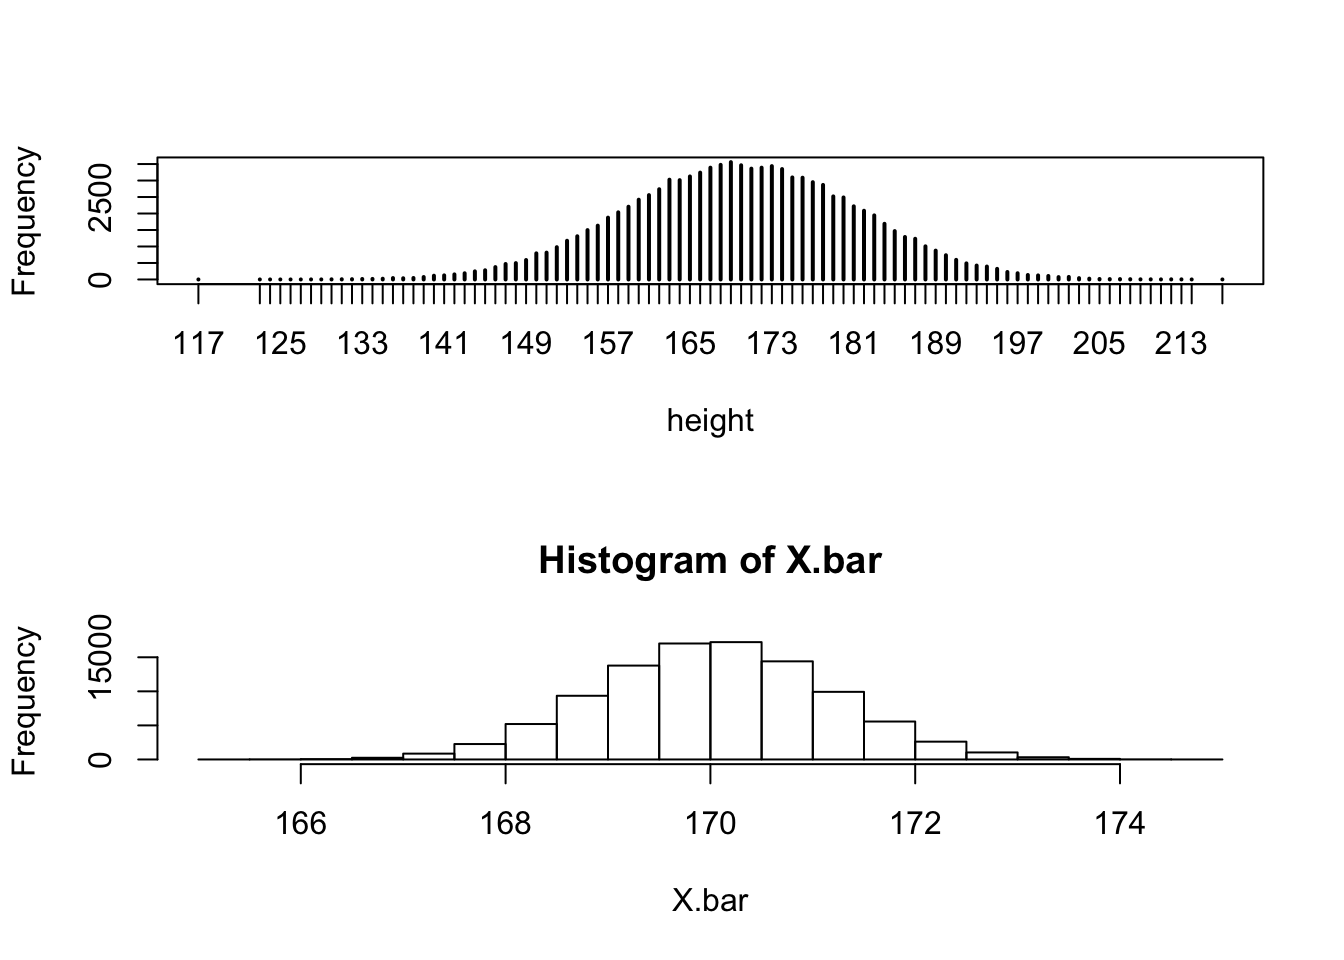
\includegraphics[width=0.6\linewidth]{statthink_files/figure-latex/SampDist6-1} 

}

\caption{Distribution of Height and the Sampling Distribution of Averages}\label{fig:SampDist6}
\end{figure}

The \texttt{R} system treats a collection of expressions enclosed within curly
brackets as one entity. Therefore, in each iteration of the ``\texttt{for}''
loop, the lines that are within the curly brackets are evaluated. In the
first line a random sample of size 100 is produced and in the second
line the average of the sample is computed and stored in the \(i\)-th
position of the sequence ``\texttt{X.bar}''. Observe that the specific position
in the sequence is referred to by using square brackets.

The program changes the original components of the sequence, from 0 to
the average of a random sample, one by one. When the loop ends all
values are changed and the sequence ``\texttt{X.bar}'' contains 100,000
evaluations of the sample average. The last line, which is outside the
curly brackets and is evaluated after the ``\texttt{for}'' loop ends, produces an
histogram of the averages that were simulated. The histogram is
presented in the lower panel of Figure~\ref{fig:SampDist6}.

Compare the distribution of the sample average to the distribution of
the heights in the population that was presented first in
Figure~\ref{fig:Prob1} and is currently presented in the upper
panel of Figure~\ref{fig:SampDist6}. Observe that both distributions are
centered at about 170 centimeters. Notice, however, that the range of
values of the sample average lies essentially between 166 and 174
centimeters, whereas the range of the distribution of heights themselves
is between 127 and 217 centimeter. Broadly speaking, the sample average
and the original measurement are centered around the same location but
the sample average is less spread.

Specifically, let us compare the expectation and standard deviation of
the sample average to the expectation and standard deviation of the
original measurement:

\begin{Shaded}
\begin{Highlighting}[]
\KeywordTok{mean}\NormalTok{(pop}\FloatTok{.1}\OperatorTok{$}\NormalTok{height)}
\end{Highlighting}
\end{Shaded}

\begin{verbatim}
## [1] 170.035
\end{verbatim}

\begin{Shaded}
\begin{Highlighting}[]
\KeywordTok{sd}\NormalTok{(pop}\FloatTok{.1}\OperatorTok{$}\NormalTok{height)}
\end{Highlighting}
\end{Shaded}

\begin{verbatim}
## [1] 11.232047
\end{verbatim}

\begin{Shaded}
\begin{Highlighting}[]
\KeywordTok{mean}\NormalTok{(X.bar)}
\end{Highlighting}
\end{Shaded}

\begin{verbatim}
## [1] 170.03283
\end{verbatim}

\begin{Shaded}
\begin{Highlighting}[]
\KeywordTok{sd}\NormalTok{(X.bar)}
\end{Highlighting}
\end{Shaded}

\begin{verbatim}
## [1] 1.1200248
\end{verbatim}

Observe that the expectation of the population and the expectation of
the sample average, are practically the same, the standard deviation of
the sample average is about 10 times smaller than the standard deviation
of the population. This result is not accidental and actually reflects a
general phenomena that will be seen below in other examples.

We may use the simulated sampling distribution in order to compute an
approximation of the probability of the sample average falling within 1
centimeter of the population mean. Let us first compute the relevant
probability and then explain the details of the computation:

\begin{Shaded}
\begin{Highlighting}[]
\KeywordTok{mean}\NormalTok{(}\KeywordTok{abs}\NormalTok{(X.bar }\OperatorTok{-}\StringTok{ }\KeywordTok{mean}\NormalTok{(pop}\FloatTok{.1}\OperatorTok{$}\NormalTok{height)) }\OperatorTok{<=}\StringTok{ }\DecValTok{1}\NormalTok{)}
\end{Highlighting}
\end{Shaded}

\begin{verbatim}
## [1] 0.62738
\end{verbatim}

Hence we get that the probability of the given event is about 62.6\%.

The object ``\texttt{X.bar}'' is a sequence of length 100,000 that contains the
simulated sample averages. This sequence represents the distribution of
the sample average. The expression
``\texttt{abs(X.bar\ -\ mean(pop.1\$height))\ \textless{}=\ 1}'' produces a sequence of logical
``\texttt{TRUE}'' or ``\texttt{FALSE}'' values, depending on the value of the sample
average being less or more than one unit away from the population mean.
The application of the function ``\texttt{mean}'' to the output of the last
expression results in the computation of the relative frequency of
\texttt{TRUE}s, which corresponds to the probability of the event of interest.

\BeginKnitrBlock{example}
\protect\hypertarget{exm:exsampdist1}{}{\label{exm:exsampdist1} }A poll for the determination of the support in the
population for a candidate was describe in
Example~\ref{exm:exrvar1}. The proportion in the population of
supporters was denoted by \(p\). A sample of size \(n=300\) was considered
in order to estimate the size of \(p\). We identified that the
distribution of \(X\), the number of supporters in the sample, is
\(\mathrm{Binomial}(300,p)\). This distribution is the sampling
distribution\footnote{Mathematically speaking, the Binomial distribution is only an
  approximation to the sampling distribution of \(X\). Actually, the
  Binomial is an exact description to the distribution only in the
  case where each subject has the chance be represented in the sample
  more than once. However, only when the size of the sample is
  comparable to the size of the population would the Binomial
  distribution fail to be an adequate approximation to the sampling
  distribution.} of \(X\). One may use the proportion in the sample of
supporters, the number of supporters in the sample divided by 300, as an
estimate to the parameter \(p\). The sampling distribution of this
quantity, \(X/300\), may be considered in order to assess the discrepancy
between the estimate and the actual value of the parameter.
\EndKnitrBlock{example}

\hypertarget{subsec:theoreticalmdls}{%
\subsection{Theoretical Models}\label{subsec:theoreticalmdls}}

Sampling distribution can also be considered in the context of
theoretical distribution models. For example, take a measurement
\(X \sim \mathrm{Binomial}(10,0.5)\) from the Binomial distribution.
Assume 64 independent measurements are produced with this distribution:
\(X_1, X_2, \ldots, X_{64}\). The sample average in this case corresponds
to the distribution of the random variable produced by averaging these
64 random variables:

\[\bar X = \frac{X_1 + X_2 + \cdots + X_{64}} {64} = \frac{1}{64}\sum_{i=1}^{64} X_i\;.\]
Again, one may wonder what is the distribution of the sample average
\(\bar X\) in this case?

We can approximate the distribution of the sample average by simulation.
The function ``\texttt{rbinom}'' produces a random sample from the Binomial
distribution. The first argument to the function is the sample size,
which we take in this example to be equal to 64. The second and third
arguments are the parameters of the Binomial distribution, 10 and 0.5 in
this case. We can use this function in the simulation:

\begin{Shaded}
\begin{Highlighting}[]
\NormalTok{X.bar <-}\StringTok{ }\KeywordTok{rep}\NormalTok{(}\DecValTok{0}\NormalTok{,}\DecValTok{10}\OperatorTok{^}\DecValTok{5}\NormalTok{)}
\ControlFlowTok{for}\NormalTok{(i }\ControlFlowTok{in} \DecValTok{1}\OperatorTok{:}\DecValTok{10}\OperatorTok{^}\DecValTok{5}\NormalTok{) \{}
\NormalTok{  X.samp <-}\StringTok{ }\KeywordTok{rbinom}\NormalTok{(}\DecValTok{64}\NormalTok{,}\DecValTok{10}\NormalTok{,}\FloatTok{0.5}\NormalTok{)}
\NormalTok{  X.bar[i] <-}\StringTok{ }\KeywordTok{mean}\NormalTok{(X.samp)}
\NormalTok{\}}
\end{Highlighting}
\end{Shaded}

Observe that in this code we created a sequence of length 100,000 with
evaluations of the sample average of 64 Binomial random variables. We
start with a sequence of zeros and in each iteration of the ``\texttt{for}'' loop
a zero is replaced by the average of a random sample of 64 Binomial
random variables.

\begin{figure}

{\centering 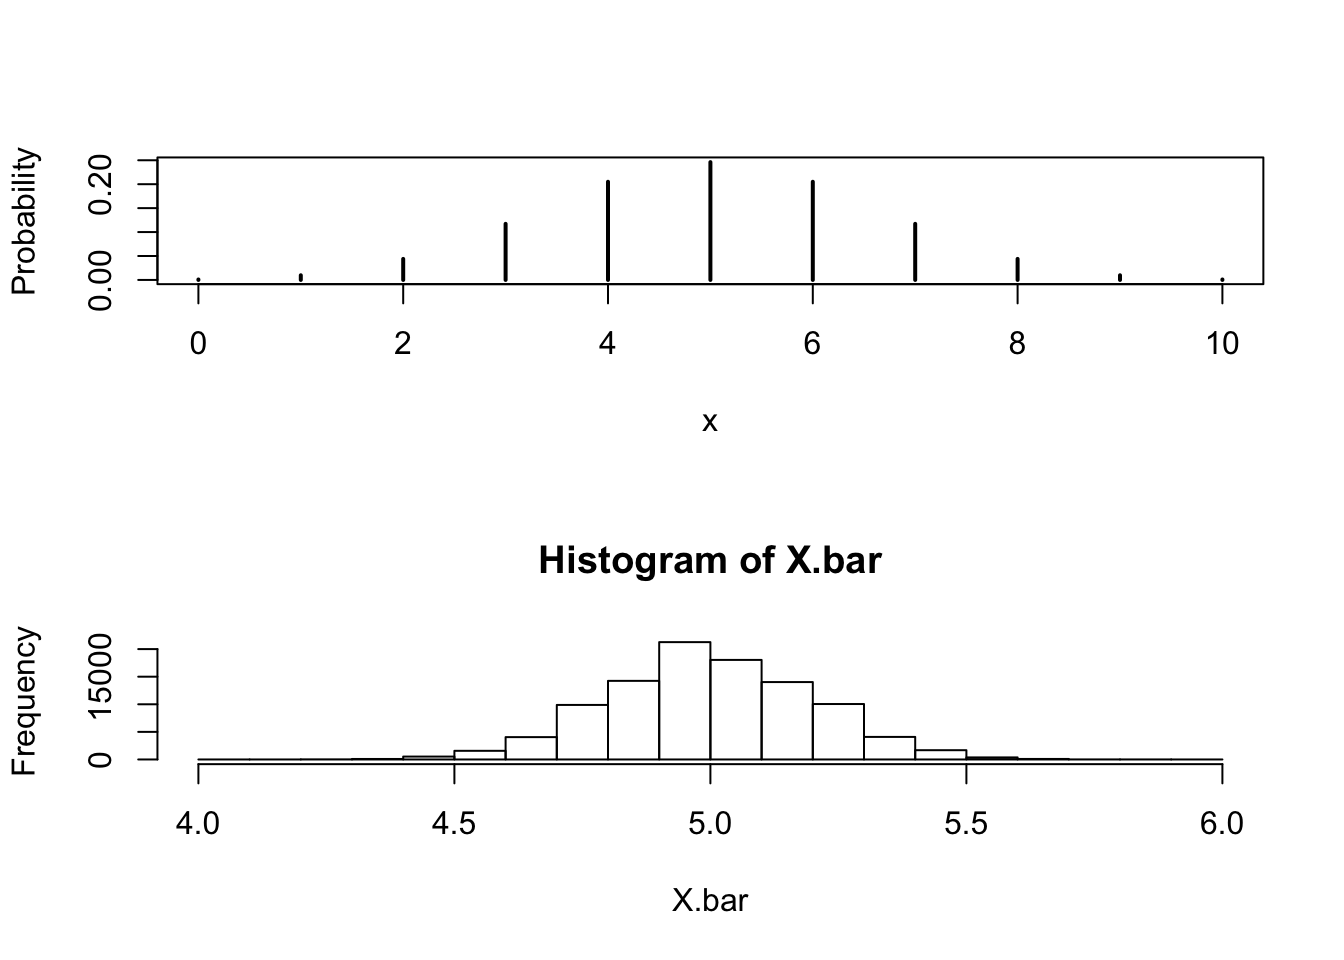
\includegraphics[width=0.6\linewidth]{statthink_files/figure-latex/SampDist7-1} 

}

\caption{Distributions of an Average and a Single Binomial(10,0.5)}\label{fig:SampDist7}
\end{figure}

Examine the sampling distribution of the Binomial average:

\begin{Shaded}
\begin{Highlighting}[]
\KeywordTok{mean}\NormalTok{(X.bar)}
\end{Highlighting}
\end{Shaded}

\begin{verbatim}
## [1] 5.0016925
\end{verbatim}

\begin{Shaded}
\begin{Highlighting}[]
\KeywordTok{sd}\NormalTok{(X.bar)}
\end{Highlighting}
\end{Shaded}

\begin{verbatim}
## [1] 0.19828121
\end{verbatim}

The histogram of the sample average is presented in the lower panel of
Figure~\ref{fig:SampDist7}. Compare it to the distribution of a single
Binomial random variable that appears in the upper panel. Notice, once
more, that the center of the two distributions coincide but the spread
of the sample average is smaller. The sample space of a single Binomial
random variable is composed of integers. The sample space of the average
of 64 Binomial random variables, on the other hand, contains many more
values and is closer to the sample space of a random variable with a
continuous distribution.

Recall that the expectation of a \(\mathrm{Binomial}(10,0.5)\) random
variable is \(\Expec(X) = 10 \cdot 0.5 = 5\) and the variance is
\(\Var(X) = 10 \cdot 0.5 \cdot 0.5 = 2.5\) (thus, the standard deviation
is \(\sqrt{2.5} = 1.581139\)). Observe that the expectation of the sample
average that we got from the simulation is essentially equal to 5 and
the standard deviation is 0.1982219.

One may prove mathematically that the expectation of the sample mean is
equal to the theoretical expectation of its components:

\[\Expec(\bar X) = \Expec(X)\;.\] The results of the simulation for the
expectation of the sample average are consistent with the mathematical
statement. The mathematical theory of probability may also be used in
order to prove that the variance of the sample average is equal to the
variance of each of the components, divided by the sample size:

\[\Var(\bar X) = \Var(X)/n\;,\] here \(n\) is the number of observations
in the sample. Specifically, in the Binomial example we get that
\(\Var(\bar X) = 2.5/64\), since the variance of a Binomial component is
2.5 and there are 64 observations. Consequently, the standard deviation
is \(\sqrt{2.5/64} = 0.1976424\), in agreement, more or less, with the
results of the simulation (that produced 0.1982219 as the standard
deviation).

Consider the problem of identifying the central interval that contains
95\% of the distribution. In the Normal distribution we were able to use
the function ``\texttt{qnorm}'' in order to compute the percentiles of the
theoretical distribution. A function that can be used for the same
purpose for simulated distribution is the function ``\texttt{quantile}''. The
first argument to this function is the sequence of simulated values of
the statistic, ``\texttt{X.bar}'' in the current case. The second argument is a
number between 0 and 1, or a sequence of such numbers:

\begin{Shaded}
\begin{Highlighting}[]
\KeywordTok{quantile}\NormalTok{(X.bar,}\KeywordTok{c}\NormalTok{(}\FloatTok{0.025}\NormalTok{,}\FloatTok{0.975}\NormalTok{))}
\end{Highlighting}
\end{Shaded}

\begin{verbatim}
##     2.5%    97.5% 
## 4.609375 5.390625
\end{verbatim}

We used the sequence ``\texttt{c(0.025,0.975)}'' as the input to the second
argument. As a result we obtained the output 4.609375, which is the
2.5\%-percentile of the sampling distribution of the average, and
5.390625, which is the 97.5\%-percentile of the sampling distribution of
the average.

Of interest is to compare these percentiles to the parallel percentiles
of the Normal distribution with the same expectation and the same
standard deviation as the average of the Binomials:

\begin{Shaded}
\begin{Highlighting}[]
\KeywordTok{qnorm}\NormalTok{(}\KeywordTok{c}\NormalTok{(}\FloatTok{0.025}\NormalTok{,}\FloatTok{0.975}\NormalTok{),}\KeywordTok{mean}\NormalTok{(X.bar),}\KeywordTok{sd}\NormalTok{(X.bar))}
\end{Highlighting}
\end{Shaded}

\begin{verbatim}
## [1] 4.6130685 5.3903165
\end{verbatim}

Observe the similarity between the percentiles of the distribution of
the average and the percentiles of the Normal distribution. This
similarity is a reflection of the Normal approximation of the sampling
distribution of the average, which is formulated in the next section
under the title: \emph{The Central Limit Theorem}.

\BeginKnitrBlock{example}
\protect\hypertarget{exm:exsampdist3}{}{\label{exm:exsampdist3} }The distribution of the number of events of radio
active decay in a second was modeled in Example~\ref{exm:exrvar3}
according to the Poisson distribution. A quantity of interest is
\(\lambda\), the expectation of that Poisson distribution. This quantity
may be estimated by measuring the total number of decays over a period
of time and dividing the outcome by the number of seconds in that period
of time. Let \(n\) be this number of second. The procedure just described
corresponds to taking the sample average of \(\mathrm{Poisson}(\lambda)\)
observations for a sample of size \(n\). The expectation of the sample
average is \(\lambda\) and the variance is \(\lambda/n\), leading to a
standard deviation of size \(\sqrt{\lambda/n}\). The Central Limit Theorem
states that the sampling distribution of this average corresponds,
approximately, to the Normal distribution with this expectation and
standard deviation.
\EndKnitrBlock{example}

\hypertarget{law-of-large-numbers-and-central-limit-theorem}{%
\section{Law of Large Numbers and Central Limit Theorem}\label{law-of-large-numbers-and-central-limit-theorem}}

The Law of Large Numbers and the Central Limit Theorem are mathematical
theorems that describe the sampling distribution of the average for
large samples.

\hypertarget{the-law-of-large-numbers}{%
\subsection{The Law of Large Numbers}\label{the-law-of-large-numbers}}

The Law of Large Numbers states that, as the sample size becomes larger,
the sampling distribution of the sample average becomes more and more
concentrated about the expectation.

Let us demonstrate the Law of Large Numbers in the context of the
Uniform distribution. Let the distribution of the measurement \(X\) be
\(\mathrm{Uniform}(3,7)\). Consider three different sample sizes \(n\):
\(n=10\), \(n=100\), and \(n=1000\). Let us carry out a simulation similar to
the simulations of the previous section. However, this time we run the
simulation for the three sample sizes in parallel:

\begin{Shaded}
\begin{Highlighting}[]
\NormalTok{unif}\FloatTok{.10}\NormalTok{ <-}\StringTok{ }\KeywordTok{rep}\NormalTok{(}\DecValTok{0}\NormalTok{,}\DecValTok{10}\OperatorTok{^}\DecValTok{5}\NormalTok{)}
\NormalTok{unif}\FloatTok{.100}\NormalTok{ <-}\StringTok{ }\KeywordTok{rep}\NormalTok{(}\DecValTok{0}\NormalTok{,}\DecValTok{10}\OperatorTok{^}\DecValTok{5}\NormalTok{)}
\NormalTok{unif}\FloatTok{.1000}\NormalTok{ <-}\StringTok{ }\KeywordTok{rep}\NormalTok{(}\DecValTok{0}\NormalTok{,}\DecValTok{10}\OperatorTok{^}\DecValTok{5}\NormalTok{)}
\ControlFlowTok{for}\NormalTok{(i }\ControlFlowTok{in} \DecValTok{1}\OperatorTok{:}\DecValTok{10}\OperatorTok{^}\DecValTok{5}\NormalTok{) \{}
\NormalTok{  X.samp}\FloatTok{.10}\NormalTok{ <-}\StringTok{ }\KeywordTok{runif}\NormalTok{(}\DecValTok{10}\NormalTok{,}\DecValTok{3}\NormalTok{,}\DecValTok{7}\NormalTok{)}
\NormalTok{  unif}\FloatTok{.10}\NormalTok{[i] <-}\StringTok{ }\KeywordTok{mean}\NormalTok{(X.samp}\FloatTok{.10}\NormalTok{)}
\NormalTok{  X.samp}\FloatTok{.100}\NormalTok{ <-}\StringTok{ }\KeywordTok{runif}\NormalTok{(}\DecValTok{100}\NormalTok{,}\DecValTok{3}\NormalTok{,}\DecValTok{7}\NormalTok{)}
\NormalTok{  unif}\FloatTok{.100}\NormalTok{[i] <-}\StringTok{ }\KeywordTok{mean}\NormalTok{(X.samp}\FloatTok{.100}\NormalTok{)}
\NormalTok{  X.samp}\FloatTok{.1000}\NormalTok{ <-}\StringTok{ }\KeywordTok{runif}\NormalTok{(}\DecValTok{1000}\NormalTok{,}\DecValTok{3}\NormalTok{,}\DecValTok{7}\NormalTok{)}
\NormalTok{  unif}\FloatTok{.1000}\NormalTok{[i] <-}\StringTok{ }\KeywordTok{mean}\NormalTok{(X.samp}\FloatTok{.1000}\NormalTok{)}
\NormalTok{\}}
\end{Highlighting}
\end{Shaded}

Observe that we have produced 3 sequences of length 100,000 each:
``\texttt{unif.10}'', ``\texttt{unif.100}'', and ``\texttt{unif.1000}''. The first sequence is an
approximation of the sampling distribution of an average of 10
independent Uniform measurements, the second approximates the sampling
distribution of an average of 100 measurements and the third the
distribution of an average of 1000 measurements. The distribution of
single measurement in each of the examples is \(\mathrm{Uniform}(3,7)\).

Consider the expectation of sample average for the three sample sizes:

\begin{Shaded}
\begin{Highlighting}[]
\KeywordTok{mean}\NormalTok{(unif}\FloatTok{.10}\NormalTok{)}
\end{Highlighting}
\end{Shaded}

\begin{verbatim}
## [1] 5.0003703
\end{verbatim}

\begin{Shaded}
\begin{Highlighting}[]
\KeywordTok{mean}\NormalTok{(unif}\FloatTok{.100}\NormalTok{)}
\end{Highlighting}
\end{Shaded}

\begin{verbatim}
## [1] 4.9999936
\end{verbatim}

\begin{Shaded}
\begin{Highlighting}[]
\KeywordTok{mean}\NormalTok{(unif}\FloatTok{.1000}\NormalTok{)}
\end{Highlighting}
\end{Shaded}

\begin{verbatim}
## [1] 4.9998528
\end{verbatim}

For all sample size the expectation of the sample average is equal to 5,
which is the expectation of the \(\mathrm{Uniform}(3,7)\) distribution.

Recall that the variance of the \(\mathrm{Uniform}(a,b)\) distribution is
\((b-a)^2/12\). Hence, the variance of the given Uniform distribution is
\(\Var(X) = (7-3)^2/12 = 16/12 \approx 1.3333\). The variances of the
sample averages are:

\begin{Shaded}
\begin{Highlighting}[]
\KeywordTok{var}\NormalTok{(unif}\FloatTok{.10}\NormalTok{)}
\end{Highlighting}
\end{Shaded}

\begin{verbatim}
## [1] 0.13331181
\end{verbatim}

\begin{Shaded}
\begin{Highlighting}[]
\KeywordTok{var}\NormalTok{(unif}\FloatTok{.100}\NormalTok{)}
\end{Highlighting}
\end{Shaded}

\begin{verbatim}
## [1] 0.013423851
\end{verbatim}

\begin{Shaded}
\begin{Highlighting}[]
\KeywordTok{var}\NormalTok{(unif}\FloatTok{.1000}\NormalTok{)}
\end{Highlighting}
\end{Shaded}

\begin{verbatim}
## [1] 0.0013441057
\end{verbatim}

Notice that the variances decrease with the increase of the sample
sizes. The decrease is according to the formula
\(\Var(\bar X) = \Var(X)/n\).

The variance is a measure of the spread of the distribution about the
expectation. The smaller the variance the more concentrated is the
distribution around the expectation. Consequently, in agreement with the
Law of Large Numbers, the larger the sample size the more concentrated
is the sampling distribution of the sample average about the
expectation.

\hypertarget{the-central-limit-theorem-clt}{%
\subsection{The Central Limit Theorem (CLT)}\label{the-central-limit-theorem-clt}}

The Law of Large Numbers states that the distribution of the sample
average tends to be more concentrated as the sample size increases. The
Central Limit Theorem (CLT in short) provides an approximation of this
distribution.

\begin{figure}

{\centering 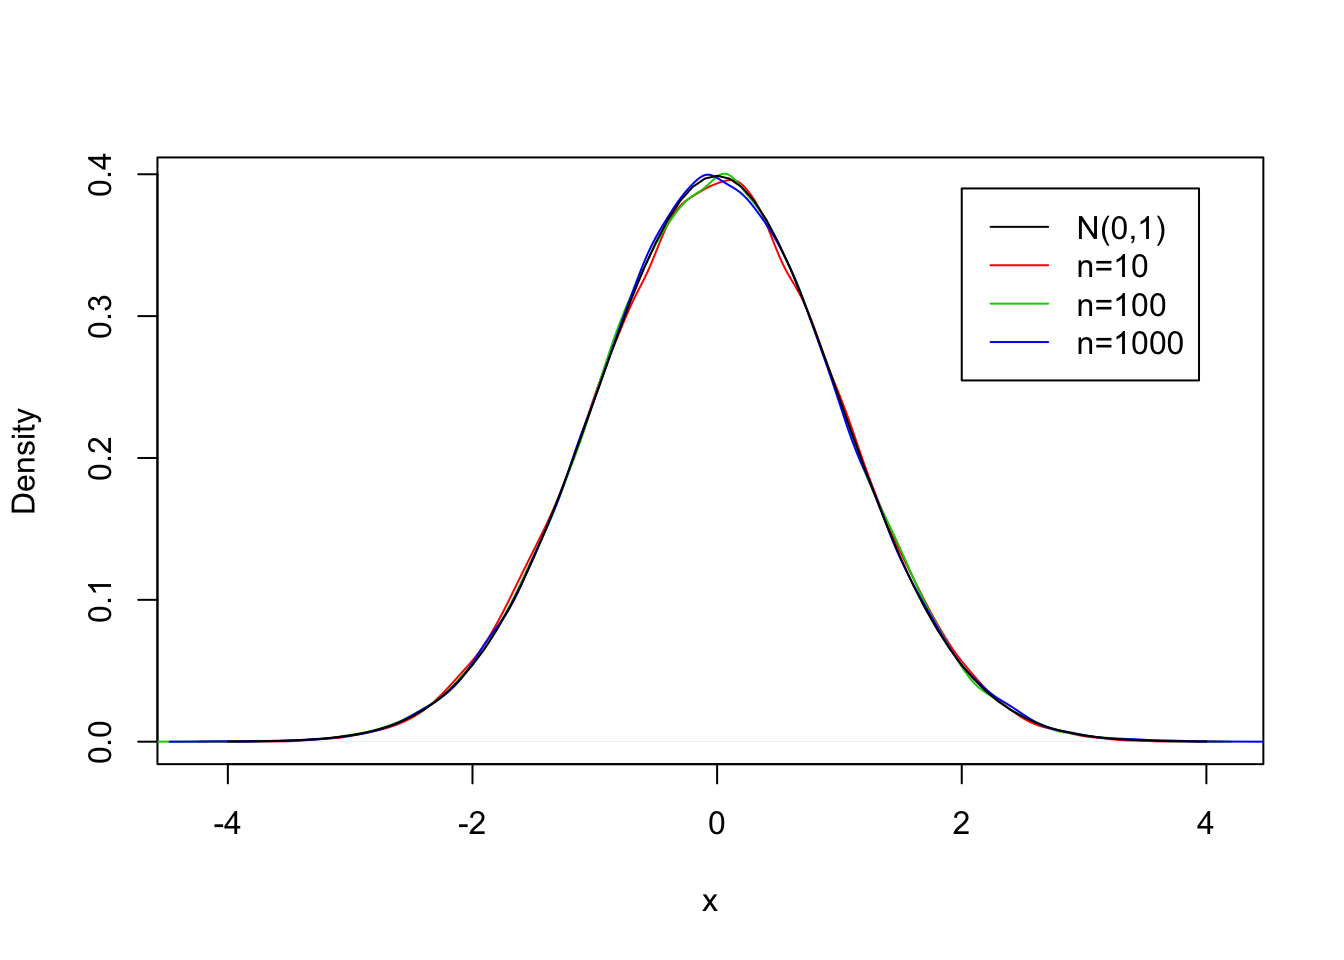
\includegraphics[width=0.6\linewidth]{statthink_files/figure-latex/SampDist8-1} 

}

\caption{The CLT for the Uniform(3,7) Distribution}\label{fig:SampDist8}
\end{figure}

The deviation between the sample average and the expectation of the
measurement tend to decreases with the increase in sample size. In order
to obtain a refined assessment of this deviation one needs to magnify
it. The appropriate way to obtain the magnification is to consider the
standardized sample average, in which the deviation of the sample
average from its expectation is divided by the standard deviation of the
sample average:

\[Z = \frac{\bar X - \Expec(\bar X)}{\sqrt{\Var(\bar X)}}\;.\]

Recall that the expectation of the sample average is equal to the
expectation of a single random variable (\(\Expec(\bar X) = \Expec(X)\))
and that the variance of the sample average is equal to the variance of
a single observation, divided by the sample size
(\(\Var(\bar X) = \Var(X)/n\)). Consequently, one may rewrite the
standardized sample average in the form:

\[Z = \frac{\bar X - \Expec(X)}{\sqrt{\Var(X)/n}}= \frac{\sqrt{n}(\bar X - \Expec(X))}{\sqrt{\Var(X)}}\;.\]
The second equality follows from placing in the numerator the square
root of \(n\) which \emph{divides} the term in the denominator. Observe that
with the increase of the sample size the decreasing difference between
the average and the expectation is magnified by the square root of \(n\).

The Central Limit Theorem states that, with the increase in sample size,
the sample average converges (after standardization) to the standard
Normal distribution.

Let us examine the Central Normal Theorem in the context of the example
of the Uniform measurement. In Figure~\ref{fig:SampDist8} you may find
the (approximated) density of the standardized average for the three
sample sizes based on the simulation that we carried out previously (as
\emph{red}, \emph{green}, and \emph{blue} lines). Along side with these densities you
may also find the theoretical density of the standard Normal
distribution (as a \emph{black} line). Observe that the four curves are
almost one on top of the other, proposing that the approximation of the
distribution of the average by the Normal distribution is good even for
a sample size as small as \(n=10\).

However, before jumping to the conclusion that the Central Limit Theorem
applies to any sample size, let us consider another example. In this
example we repeat the same simulation that we did with the Uniform
distribution, but this time we take \(\mathrm{Exponential}(0.5)\)
measurements instead:

\begin{Shaded}
\begin{Highlighting}[]
\NormalTok{exp}\FloatTok{.10}\NormalTok{ <-}\StringTok{ }\KeywordTok{rep}\NormalTok{(}\DecValTok{0}\NormalTok{,}\DecValTok{10}\OperatorTok{^}\DecValTok{5}\NormalTok{)}
\NormalTok{exp}\FloatTok{.100}\NormalTok{ <-}\StringTok{ }\KeywordTok{rep}\NormalTok{(}\DecValTok{0}\NormalTok{,}\DecValTok{10}\OperatorTok{^}\DecValTok{5}\NormalTok{)}
\NormalTok{exp}\FloatTok{.1000}\NormalTok{ <-}\StringTok{ }\KeywordTok{rep}\NormalTok{(}\DecValTok{0}\NormalTok{,}\DecValTok{10}\OperatorTok{^}\DecValTok{5}\NormalTok{)}
\ControlFlowTok{for}\NormalTok{(i }\ControlFlowTok{in} \DecValTok{1}\OperatorTok{:}\DecValTok{10}\OperatorTok{^}\DecValTok{5}\NormalTok{) \{}
\NormalTok{  X.samp}\FloatTok{.10}\NormalTok{ <-}\StringTok{ }\KeywordTok{rexp}\NormalTok{(}\DecValTok{10}\NormalTok{,}\FloatTok{0.5}\NormalTok{)}
\NormalTok{  exp}\FloatTok{.10}\NormalTok{[i] <-}\StringTok{ }\KeywordTok{mean}\NormalTok{(X.samp}\FloatTok{.10}\NormalTok{)}
\NormalTok{  X.samp}\FloatTok{.100}\NormalTok{ <-}\StringTok{ }\KeywordTok{rexp}\NormalTok{(}\DecValTok{100}\NormalTok{,}\FloatTok{0.5}\NormalTok{)}
\NormalTok{  exp}\FloatTok{.100}\NormalTok{[i] <-}\StringTok{ }\KeywordTok{mean}\NormalTok{(X.samp}\FloatTok{.100}\NormalTok{)}
\NormalTok{  X.samp}\FloatTok{.1000}\NormalTok{ <-}\StringTok{ }\KeywordTok{rexp}\NormalTok{(}\DecValTok{1000}\NormalTok{,}\FloatTok{0.5}\NormalTok{)}
\NormalTok{  exp}\FloatTok{.1000}\NormalTok{[i] <-}\StringTok{ }\KeywordTok{mean}\NormalTok{(X.samp}\FloatTok{.1000}\NormalTok{)}
\NormalTok{\}}
\end{Highlighting}
\end{Shaded}

\begin{figure}

{\centering 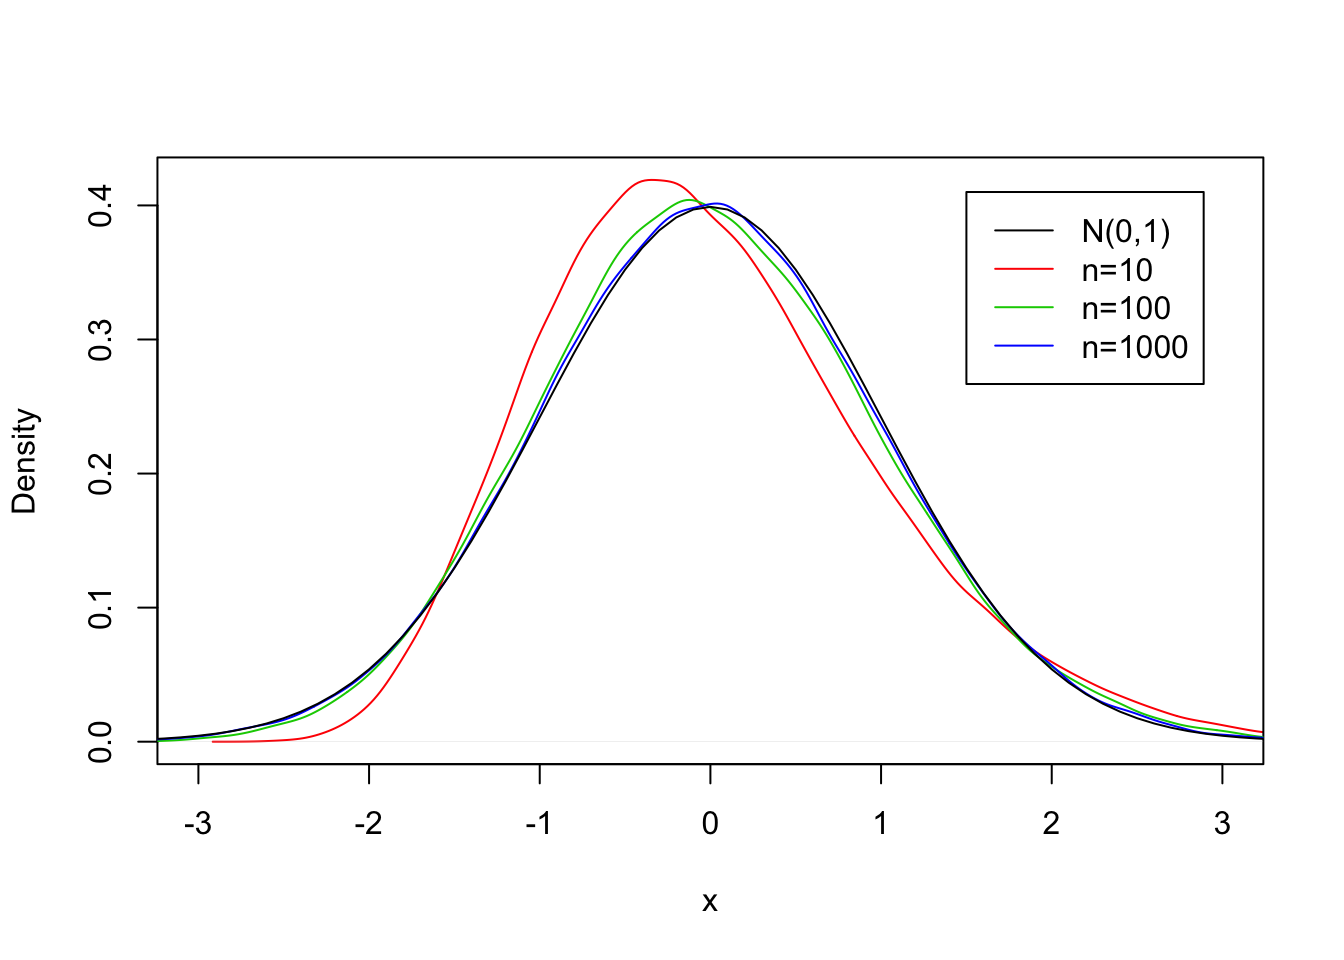
\includegraphics[width=0.6\linewidth]{statthink_files/figure-latex/SampDist9-1} 

}

\caption{The CLT for the Exponential(0.5) Distribution}\label{fig:SampDist9}
\end{figure}

The expectation of an \(\mathrm{Exponential}(0.5)\) random variable is
\(\Expec(X) = 1/\lambda = 1/0.5 = 2\) and the variance is
\(\Var(X) = 1/\lambda^2 = 1/(0.5)^2 = 4\). Observe below that the
expectations of the sample averages are equal to the expectation of the
measurement and the variances of the sample averages follow the relation
\(\Var(\bar X) = \Var (X)/n\):

\begin{Shaded}
\begin{Highlighting}[]
\KeywordTok{mean}\NormalTok{(exp}\FloatTok{.10}\NormalTok{)}
\end{Highlighting}
\end{Shaded}

\begin{verbatim}
## [1] 1.9993274
\end{verbatim}

\begin{Shaded}
\begin{Highlighting}[]
\KeywordTok{mean}\NormalTok{(exp}\FloatTok{.100}\NormalTok{)}
\end{Highlighting}
\end{Shaded}

\begin{verbatim}
## [1] 2.0001339
\end{verbatim}

\begin{Shaded}
\begin{Highlighting}[]
\KeywordTok{mean}\NormalTok{(exp}\FloatTok{.1000}\NormalTok{)}
\end{Highlighting}
\end{Shaded}

\begin{verbatim}
## [1] 2.0000449
\end{verbatim}

So the expectations of the sample average are all equal to 2. For the
variance we get:

\begin{Shaded}
\begin{Highlighting}[]
\KeywordTok{var}\NormalTok{(exp}\FloatTok{.10}\NormalTok{)}
\end{Highlighting}
\end{Shaded}

\begin{verbatim}
## [1] 0.39901428
\end{verbatim}

\begin{Shaded}
\begin{Highlighting}[]
\KeywordTok{var}\NormalTok{(exp}\FloatTok{.100}\NormalTok{)}
\end{Highlighting}
\end{Shaded}

\begin{verbatim}
## [1] 0.040383536
\end{verbatim}

\begin{Shaded}
\begin{Highlighting}[]
\KeywordTok{var}\NormalTok{(exp}\FloatTok{.1000}\NormalTok{)}
\end{Highlighting}
\end{Shaded}

\begin{verbatim}
## [1] 0.0039863432
\end{verbatim}

Which is in agreement with the decrease proposed by the theory,

However, when one examines the densities of the sample averages in
Figure~@reF(fig:SampDist9) one may see a clear distinction between the
sampling distribution of the average for a sample of size 10 and the
normal distribution (compare the \emph{red} curve to the \emph{black} curve. The
match between the \emph{green} curve that corresponds to a sample of size
\(n=100\) and the \emph{black} line is better, but not perfect. When the sample
size is as large as \(n=1000\) (the \emph{blue} curve) then the agreement with
the normal curve is very good.

\hypertarget{applying-the-central-limit-theorem}{%
\subsection{Applying the Central Limit Theorem}\label{applying-the-central-limit-theorem}}

The conclusion of the Central Limit Theorem is that the sampling
distribution of the sample average can be approximated by the Normal
distribution, regardless what is the distribution of the original
measurement, but provided that the sample size is large enough. This
statement is very important, since it allows us, in the context of the
sample average, to carry out probabilistic computations using the Normal
distribution even if we do not know the actual distribution of the
measurement. All we need to know for the computation are the expectation
of the measurement, its variance (or standard deviation) and the sample
size.

The theorem can be applied whenever probability computations associated
with the sampling distribution of the average are required. The
computation of the approximation is carried out by using the Normal
distribution with the same expectation and the same standard deviation
as the sample average.

An example of such computation was conducted in
Subsection~\ref{subsec:theoreticalmdls} where the central interval that
contains 95\% of the sampling distribution of a Binomial average was
required. The 2.5\%- and the 97.5\%-percentiles of the Normal distribution
with the same expectation and variance as the sample average produced
boundaries for the interval. These boundaries were in good agreement
with the boundaries produced by the simulation. More examples will be
provided in the Solved Exercises of this chapter and the next one.

With all its usefulness, one should treat the Central Limit Theorem with
a grain of salt. The approximation may be valid for large samples, but
may be bad for samples that are not large enough. When the sample is
small a careless application of the Central Limit Theorem may produce
misleading conclusions.

\hypertarget{SampDistEx}{%
\section{Exercises}\label{SampDistEx}}

\BeginKnitrBlock{exercise}
\protect\hypertarget{exr:ex1sampdist}{}{\label{exr:ex1sampdist} }The file ``\texttt{pop2.csv}'' contains information associated
to the blood pressure of an imaginary population of size 100,000. The
file can be found on the internet
(\url{http://pluto.huji.ac.il/~msby/StatThink/Datasets/pop2.csv}). The
variables in this file are:

\begin{description}
\item[id:]
A numerical variable. A 7 digits number that serves as a unique
identifier of the subject.
\item[sex:]
A factor variable. The sex of each subject. The values are either
``\texttt{MALE}'' or ``\texttt{FEMALE}''.
\item[age:]
A numerical variable. The age of each subject.
\item[bmi:]
A numerical variable. The body mass index of each subject.
\item[systolic:]
A numerical variable. The systolic blood pressure of each subject.
\item[diastolic:]
A numerical variable. The diastolic blood pressure of each subject.
\item[group:]
A factor variable. The blood pressure category of each subject. The
values are ``\texttt{NORMAL}'' both the systolic blood pressure is within its
normal range (between 90 and 139) and the diastolic blood pressure
is within its normal range (between 60 and 89). The value is
``\texttt{HIGH}'' if either measurements of blood pressure are above their
normal upper limits and it is ``\texttt{LOW}'' if either measurements are
below their normal lower limits.
\end{description}

Our goal in this question is to investigate the sampling distribution of
the sample average of the variable ``\texttt{bmi}''. We assume a sample of size
\(n=150\).

\begin{enumerate}
\def\labelenumi{\arabic{enumi}.}
\item
  Compute the population average of the variable ``\texttt{bmi}''.
\item
  Compute the population standard deviation of the variable ``\texttt{bmi}''.
\item
  Compute the expectation of the sampling distribution for the sample
  average of the variable.
\item
  Compute the standard deviation of the sampling distribution for the
  sample average of the variable.
\item
  Identify, using simulations, the central region that contains 80\% of
  the sampling distribution of the sample average.
\item
  Identify, using the Central Limit Theorem, an approximation of the
  central region that contains 80\% of the sampling distribution of the
  sample average.
\end{enumerate}
\EndKnitrBlock{exercise}

\BeginKnitrBlock{exercise}
\protect\hypertarget{exr:unnamed-chunk-109}{}{\label{exr:unnamed-chunk-109} }A subatomic particle hits a linear detector at random
locations. The length of the detector is 10 nm and the hits are
uniformly distributed. The location of 25 random hits, measured from a
specified endpoint of the interval, are marked and the average of the
location computed.

\begin{enumerate}
\def\labelenumi{\arabic{enumi}.}
\item
  What is the expectation of the average location?
\item
  What is the standard deviation of the average location?
\item
  Use the Central Limit Theorem in order to approximate the
  probability the average location is in the left-most third of the
  linear detector.
\item
  The central region that contains 99\% of the distribution of the
  average is of the form \(5 \pm c\). Use the Central Limit Theorem in
  order to approximate the value of c.
\end{enumerate}
\EndKnitrBlock{exercise}

\hypertarget{summary-6}{%
\section{Summary}\label{summary-6}}

\hypertarget{glossary}{%
\subsection*{Glossary}\label{glossary}}


\begin{description}
\item[Random Sample:]
The probabilistic model for the values of a measurements in the
sample, before the measurement is taken.
\item[Sampling Distribution:]
The distribution of a random sample.
\item[Sampling Distribution of a Statistic:]
A statistic is a function of the data; i.e.~a formula applied to the
data. The statistic becomes a random variable when the formula is
applied to a random sample. The distribution of this random
variable, which is inherited from the distribution of the sample, is
its sampling distribution.
\item[Sampling Distribution of the Sample Average:]
The distribution of the sample average, considered as a random
variable.
\item[The Law of Large Numbers:]
A mathematical result regarding the sampling distribution of the
sample average. States that the distribution of the average of
measurements is highly concentrated in the vicinity of the
expectation of a measurement when the sample size is large.
\item[The Central Limit Theorem:]
A mathematical result regarding the sampling distribution of the
sample average. States that the distribution of the average is
approximately Normal when the sample size is large.
\end{description}

\hypertarget{discussion-in-the-forum}{%
\subsection*{Discussion in the Forum}\label{discussion-in-the-forum}}


Limit theorems in mathematics deal with the convergence of some property
to a limit as some indexing parameter goes to infinity. The Law of Large
Numbers and the Central Limit Theorem are examples of limit theorems.
The property they consider is the sampling distribution of the sample
average. The indexing parameter that goes to infinity is the sample size
\(n\).

Some people say that the Law of Large Numbers and the Central Limit
Theorem are useless for practical purposes. These theorems deal with a
sample size that goes to infinity. However, all sample sizes one finds
in reality are necessarily finite. What is your opinion?

When forming your answer to this question you may give an example of a
situation from your own field of interest in which conclusions of an
abstract mathematical theory are used in order to solve a practical
problem. Identify the merits and weaknesses of the application of the
mathematical theory.

For example, in making statistical inference one frequently needs to
make statements regarding the sampling distribution of the sample
average. For instant, one may want to identify the central region that
contains 95\% of the distribution. The Normal distribution is used in the
computation. The justification is the Central Limit Theorem.

\hypertarget{summary-of-formulas}{%
\subsection*{Summary of Formulas}\label{summary-of-formulas}}


\begin{description}
\item[Expectation of the sample average:]
\(\Expec(\bar X) = \Expec(X)\)
\item[Variance of the sample average:]
\(\Var(\bar X) = \Var(X)/n\)
\end{description}

\hypertarget{overview-and-integration}{%
\chapter{Overview and Integration}\label{overview-and-integration}}

\hypertarget{student-learning-objective-4}{%
\section{Student Learning Objective}\label{student-learning-objective-4}}

This section provides an overview of the concepts and methods that where
presented in the first part of the book. We attempt to relate them to
each other and put them in prospective. Some problems are provided. The
solutions to these problems require combinations of many of the tools
that were presented in previous chapters. By the end of this chapter,
the student should be able to:

\begin{itemize}
\item
  Have a better understanding of the relation between descriptive
  statistics, probability, and inferential statistics.
\item
  Distinguish between the different uses of the concept of
  variability.
\item
  Integrate the tools that were given in the first part of the book in
  order to solve complex problems.
\end{itemize}

\hypertarget{an-overview}{%
\section{An Overview}\label{an-overview}}

The purpose of the first part of the book was to introduce the
fundamentals of statistics and teach the concepts of probability which
are essential for the understanding of the statistical procedures that
are used to analyze data. These procedures are presented and discussed
in the second part of the book.

Data is typically obtained by selecting a sample from a population and
taking measurements on the sample. There are many ways to select a
sample, but all methods for such selection should not violate the most
important characteristic that a sample should posses, namely that it
represents the population it came from. In this book we concentrate on
simple random sampling. However, the reader should be aware of the fact
that other sampling designs exist and may be more appropriate in
specific applications. Given the sampled data, the main concern of the
science of statistics is in making inference on the parameter of the
population on the basis of the data collected. Such inferences are
carried out with the aid of statistics, which are functions of the data.

Data is frequently stored in the format of a data frame, in which
columns are the measured variable and the rows are the observations
associated with the selected sample. The main types of variables are
numeric, either discrete or not, and factors. We learned how one can
produce data frames and read data into \texttt{R} for further analysis.

Statistics is geared towards dealing with variability. Variability may
emerge in different forms and for different reasons. It can be
summarized, analyzed and handled with many tools. Frequently, the same
tool, or tools that have much resemblance to each other, may be applied
in different settings and for different forms of variability. In order
not to loose track it is important to understand in each scenario the
source and nature of the variability that is being examined.

An important split in term of the source of variability is between
descriptive statistics and probability. Descriptive statistics examines
the distribution of data. The frame of reference is the data itself.
Plots, such as the bar plots, histograms and box plot; tables, such as
the frequency and relative frequency as well as the cumulative relative
frequency; and numerical summaries, such as the mean, median and
standard deviation, can all serve in order to understand the
distribution of the given data set.

In probability, on the other hand, the frame of reference is not the
data at hand but, instead, it is all data sets that could have been
sampled (the sample space of the sampling distribution). One may use
similar plots, tables, and numerical summaries in order to analyze the
distribution of functions of the sample (statistics), but the meaning of
the analysis is different. As a matter of fact, the relevance of the
probabilistic analysis to the data actually sampled is indirect. The
given sample is only one realization within the sample space among all
possible realizations. In the probabilistic context there is no special
role to the observed realization in comparison to all other potential
realizations.

The fact that the relation between probabilistic variability and the
observed data is not direct does not make the relation unimportant. On
the contrary, this indirect relation is the basis for making statistical
inference. In statistical inference the characteristics of the data may
be used in order to extrapolate from the sampled data to the entire
population. Probabilistic description of the distribution of the sample
is then used in order to assess the reliability of the extrapolation.
For example, one may try to estimate the value of population parameters,
such as the population average and the population standard deviation, on
the basis of the parallel characteristics of the data. The variability
of the sampling distribution is used in order to quantify the accuracy
of this estimation. (See Example 5 below.)

Statistics, like many other empirically driven forms of science, uses
theoretical modeling for assessing and interpreting observational data.
In statistics this modeling component usually takes the form of a
probabilistic model for the measurements as random variables. In the
first part of this book we have encountered several such models. The
model of simple sampling assumed that each subset of a given size from
the population has equal probability to be selected as the sample.
Other, more structured models, assumed a specific form to the
distribution of the measurements. The examples we considered were the
Binomial, the Poisson, the Uniform, the Exponential and the Normal
distributions. Many more models may be found in the literature and may
be applied when appropriate. Some of these other models have \texttt{R}
functions that can be used in order to compute the distribution and
produce simulations.

A statistic is a function of sampled data that is used for making
statistical inference. When a statistic, such as the average, is
computed on a random sample then the outcome, from a probabilistic point
of view, is a random variable. The distribution of this random variable
depends on the distribution of the measurements that form the sample but
is not identical to that distribution. Hence, for example, the
distribution of an average of a sample from the Uniform distribution
does not follow the Uniform distribution. In general, the relation
between the distribution of a measurement and the distribution of a
statistic computed from a sample that is generated from that
distribution may be complex. Luckily, in the case of the sample average
the relation is rather simple, at least for samples that are large
enough.

The Central Limit Theorem provides an approximation of the distribution
of the sample average that typically improves with the increase in
sample size. The expectation of the sample average is equal to the
expectation of a single measurement and the variance is equal to the
variance of a single measurement, divided by the sample size. The
Central Limit Theorem adds to this observation the statement that the
distribution of the sample average may be approximated by the Normal
distribution (with the same expectation and standard deviation as those
of the sample average). This approximation is valid for practically any
distribution of the measurement. The conclusion is, at least in the case
of the sample average, that the distribution of the statistic depends on
the underlying distribution of the measurements only through their
expectation and variance but not through other characteristics of the
distribution.

The conclusion of the theorem extends to quantities proportional to the
sample average. Therefore, since the sum of the sample is obtained by
multiplying the sample average by the sample size \(n\), we get that the
theorem can be used in order to approximate the distribution of sums. As
a matter of fact, the theorem may be generalized much further. For
example, it may be shown to hold for a smooth function of the sample
average, thereby increasing the applicability of the theorem and its
importance.

In the next section we will solve some practical problems. In order to
solve these problems you are required to be familiar with the concepts
and tools that were introduced throughout the first part of the book.
Hence, we strongly recommend that you read again and review all the
chapters of the book that preceded this one before moving on to the next
section.

\hypertarget{integrated-applications}{%
\section{Integrated Applications}\label{integrated-applications}}

The main message of the Central Limit Theorem is that for the sample
average we may compute probabilities based on the Normal distribution
and obtain reasonable approximations, provided that the sample size is
not too small. All we need to figure out for the computations are the
expectation and variance of the underlying measurement. Otherwise, the
exact distribution of that measurement is irrelevant. Let us demonstrate
the applicability of the Central Limit Theorem in two examples.

\hypertarget{example-1}{%
\subsection{Example 1}\label{example-1}}

A study involving stress is done on a college campus among the students.
The stress scores follow a (continuous) Uniform distribution with the
lowest stress score equal to 1 and the highest equal to 5. Using a
sample of 75 students, find:

\begin{enumerate}
\def\labelenumi{\arabic{enumi}.}
\item
  The probability that the average stress score for the 75 students is
  less than 2.
\item
  The 90th percentile for the average stress score for the 75
  students.
\item
  The probability that the total of the 75 stress scores is less
  than 200.
\item
  The 90th percentile for the total stress score for the 75 students.
\end{enumerate}

\hypertarget{solution}{%
\subsection*{Solution:}\label{solution}}


Denote by \(X\) the stress score of a random student. We are given that
\(X \sim \mathrm{Uniform}(1,5)\). We use the formulas
\(\Expec(X) = (a+b)/2\) and \(\Var(X) = (b-a)^2/12\) in order to obtain the
expectation and variance of a single observation and then we use the
relations \(\Expec(\bar X) = \Expec(X)\) and \(\Var(\bar X) = \Var(X)/n\) to
translated these results to the expectation and variance of the sample
average:

\begin{Shaded}
\begin{Highlighting}[]
\NormalTok{a <-}\StringTok{ }\DecValTok{1}
\NormalTok{b <-}\StringTok{ }\DecValTok{5}
\NormalTok{n <-}\StringTok{ }\DecValTok{75}
\NormalTok{mu.bar <-}\StringTok{ }\NormalTok{(a}\OperatorTok{+}\NormalTok{b)}\OperatorTok{/}\DecValTok{2}
\NormalTok{sig.bar <-}\StringTok{ }\KeywordTok{sqrt}\NormalTok{((b}\OperatorTok{-}\NormalTok{a)}\OperatorTok{^}\DecValTok{2}\OperatorTok{/}\NormalTok{(}\DecValTok{12}\OperatorTok{*}\NormalTok{n))}
\NormalTok{mu.bar}
\end{Highlighting}
\end{Shaded}

\begin{verbatim}
## [1] 3
\end{verbatim}

\begin{Shaded}
\begin{Highlighting}[]
\NormalTok{sig.bar}
\end{Highlighting}
\end{Shaded}

\begin{verbatim}
## [1] 0.13333333
\end{verbatim}

After obtaining the expectation and the variance of the sample average
we can forget about the Uniform distribution and proceed only with the
\texttt{R} functions that are related to the Normal distribution. By the
Central Limit Theorem we get that the distribution of the sample average
is approximately \(\mathrm{Normal}(\mu, \sigma^2)\), with \(\mu\) = \texttt{mu.bar}
and \(\sigma\) = \texttt{sig.bar}.

In the Question 1.1 we are asked to find the value of the cumulative
distribution function of the sample average at \(x=2\):

\begin{Shaded}
\begin{Highlighting}[]
\KeywordTok{pnorm}\NormalTok{(}\DecValTok{2}\NormalTok{,mu.bar,sig.bar)}
\end{Highlighting}
\end{Shaded}

\begin{verbatim}
## [1] 3.1908917e-14
\end{verbatim}

The goal of Question 1.2 is to identify the 90\%-percentile of the sample
average:

\begin{Shaded}
\begin{Highlighting}[]
\KeywordTok{qnorm}\NormalTok{(}\FloatTok{0.9}\NormalTok{,mu.bar,sig.bar)}
\end{Highlighting}
\end{Shaded}

\begin{verbatim}
## [1] 3.1708735
\end{verbatim}

The sample average is equal to the total sum divided by the number of
observations, \(n=75\) in this example. The total sum is less than 200 if,
and only if the average is less than \(200/n\). Therefore, for Question
1.3:

\begin{Shaded}
\begin{Highlighting}[]
\KeywordTok{pnorm}\NormalTok{(}\DecValTok{200}\OperatorTok{/}\NormalTok{n,mu.bar,sig.bar)}
\end{Highlighting}
\end{Shaded}

\begin{verbatim}
## [1] 0.0062096653
\end{verbatim}

Finally, if 90\% of the distribution of the average is less that 3.170874
then 90\% of the distribution of the total sum is less than
\(3.170874\, n\). In Question 1.4 we get:

\begin{Shaded}
\begin{Highlighting}[]
\NormalTok{n}\OperatorTok{*}\KeywordTok{qnorm}\NormalTok{(}\FloatTok{0.9}\NormalTok{,mu.bar,sig.bar)}
\end{Highlighting}
\end{Shaded}

\begin{verbatim}
## [1] 237.81552
\end{verbatim}

\hypertarget{example-2}{%
\subsection{Example 2}\label{example-2}}

Consider again the same stress study that was described in Example~1 and
answer the same questions. However, this time assume that the stress
score may obtain only the values 1, 2, 3, 4 or 5, with the same
likelihood for obtaining each of the values.

\hypertarget{solution-1}{%
\subsection*{Solution:}\label{solution-1}}


Denote again by \(X\) the stress score of a random student. The modified
distribution states that the sample space of \(X\) are the integers
\(\{1, 2, 3, 4, 5\}\), with equal probability for each value. Since the
probabilities must sum to 1 we get that \(\Prob(X = x) = 1/5\), for all
\(x\) in the sample space. In principle we may repeat the steps of the
solution of previous example, substituting the expectation and standard
deviation of the continuous measurement by the discrete counterpart:

\begin{Shaded}
\begin{Highlighting}[]
\NormalTok{x <-}\StringTok{ }\DecValTok{1}\OperatorTok{:}\DecValTok{5}
\NormalTok{p <-}\StringTok{ }\KeywordTok{rep}\NormalTok{(}\DecValTok{1}\OperatorTok{/}\DecValTok{5}\NormalTok{,}\DecValTok{5}\NormalTok{)}
\NormalTok{n <-}\StringTok{ }\DecValTok{75}
\NormalTok{mu.X <-}\StringTok{ }\KeywordTok{sum}\NormalTok{(x}\OperatorTok{*}\NormalTok{p)}
\NormalTok{sig.X <-}\StringTok{ }\KeywordTok{sum}\NormalTok{((x}\OperatorTok{-}\NormalTok{mu.X)}\OperatorTok{^}\DecValTok{2}\OperatorTok{*}\NormalTok{p)}
\NormalTok{mu.bar <-}\StringTok{ }\NormalTok{mu.X}
\NormalTok{sig.bar <-}\StringTok{ }\KeywordTok{sqrt}\NormalTok{(sig.X}\OperatorTok{/}\NormalTok{n)}
\NormalTok{mu.bar}
\end{Highlighting}
\end{Shaded}

\begin{verbatim}
## [1] 3
\end{verbatim}

\begin{Shaded}
\begin{Highlighting}[]
\NormalTok{sig.bar}
\end{Highlighting}
\end{Shaded}

\begin{verbatim}
## [1] 0.16329932
\end{verbatim}

Notice that the expectation of the sample average is the same as before
but the standard deviation is somewhat larger due to the larger variance
in the distribution of a single response.

We may apply the Central Limit Theorem again in order to conclude that
distribution of the average is approximately
\(\mathrm{Normal}(\mu, \sigma^2)\), with \(\mu\) = \texttt{mu.bar} as before and
for the new \(\sigma\) = \texttt{sig.bar}.

For Question 2.1 we compote that the cumulative distribution function of
the sample average at \(x=2\) is approximately equal:

\begin{Shaded}
\begin{Highlighting}[]
\KeywordTok{pnorm}\NormalTok{(}\DecValTok{2}\NormalTok{,mu.bar,sig.bar)}
\end{Highlighting}
\end{Shaded}

\begin{verbatim}
## [1] 4.5706492e-10
\end{verbatim}

and the 90\%-percentile is:

\begin{Shaded}
\begin{Highlighting}[]
\KeywordTok{qnorm}\NormalTok{(}\FloatTok{0.9}\NormalTok{,mu.bar,sig.bar)}
\end{Highlighting}
\end{Shaded}

\begin{verbatim}
## [1] 3.2092765
\end{verbatim}

which produces the answer to Question~2.2.

Similarly to the solution of Question~1.3 we may conclude that the total
sum is less than 200 if, and only if the average is less than \(200/n\).
Therefore, for Question 2.3:

\begin{Shaded}
\begin{Highlighting}[]
\KeywordTok{pnorm}\NormalTok{(}\DecValTok{200}\OperatorTok{/}\NormalTok{n,mu.bar,sig.bar)}
\end{Highlighting}
\end{Shaded}

\begin{verbatim}
## [1] 0.020613417
\end{verbatim}

Observe that in the current version of the question we have the score is
integer-valued. Clearly, the sum of scores is also integer valued. Hence
we may choose to apply the continuity correction for the Normal
approximation whereby we approximate the probability that the sum is
less than 200 (i.e.~is less than or equal to 199) by the probability
that a Normal random variable is less than or equal to 199.5.
Translating this event back to the scale of the average we get the
approximation\footnote{As a matter of fact, the continuity correction could have been
  applied in the previous two sections as well, since the sample
  average has a discrete distribution.}:

\begin{Shaded}
\begin{Highlighting}[]
\KeywordTok{pnorm}\NormalTok{(}\FloatTok{199.5}\OperatorTok{/}\NormalTok{n,mu.bar,sig.bar)}
\end{Highlighting}
\end{Shaded}

\begin{verbatim}
## [1] 0.018668208
\end{verbatim}

Finally, if 90\% of the distribution of the average is less that 3.170874
then 90\% of the distribution of the total sum is less than \(3.170874 n\).
Therefore:

\begin{Shaded}
\begin{Highlighting}[]
\NormalTok{n}\OperatorTok{*}\KeywordTok{qnorm}\NormalTok{(}\FloatTok{0.9}\NormalTok{,mu.bar,sig.bar)}
\end{Highlighting}
\end{Shaded}

\begin{verbatim}
## [1] 240.69574
\end{verbatim}

or, after rounding to the nearest integer we get for Question 2.4 the
answer 241.

\hypertarget{example-3}{%
\subsection{Example 3}\label{example-3}}

Suppose that a market research analyst for a cellular phone company
conducts a study of their customers who exceed the time allowance
included on their basic cellular phone contract. The analyst finds that
for those customers who exceed the time included in their basic
contract, the excess time used follows an exponential distribution with
a mean of 22 minutes. Consider a random sample of 80 customers and find

\begin{enumerate}
\def\labelenumi{\arabic{enumi}.}
\item
  The probability that the average excess time used by the 80
  customers in the sample is longer than 20 minutes.
\item
  The 95th percentile for the average excess time for samples of 80
  customers who exceed their basic contract time allowances.
\end{enumerate}

\hypertarget{solution-2}{%
\subsection*{Solution:}\label{solution-2}}


Let \(X\) be the excess time for customers who exceed the time included in
their basic contract. We are told that
\(X \sim \mathrm{Exponential}(\lambda)\). For the Exponential distribution
\(\Expec(X) = 1/\lambda\). Hence, given that \(\Expec(X) = 22\) we can
conclude that \(\lambda = 1/22\). For the Exponential we also have that
\(\Var(X) = 1/\lambda^2\). Therefore:

\begin{Shaded}
\begin{Highlighting}[]
\NormalTok{lam <-}\StringTok{ }\DecValTok{1}\OperatorTok{/}\DecValTok{22}
\NormalTok{n <-}\StringTok{ }\DecValTok{80}
\NormalTok{mu.bar <-}\StringTok{ }\DecValTok{1}\OperatorTok{/}\NormalTok{lam}
\NormalTok{sig.bar <-}\StringTok{ }\KeywordTok{sqrt}\NormalTok{(}\DecValTok{1}\OperatorTok{/}\NormalTok{(lam}\OperatorTok{^}\DecValTok{2}\OperatorTok{*}\NormalTok{n))}
\NormalTok{mu.bar}
\end{Highlighting}
\end{Shaded}

\begin{verbatim}
## [1] 22
\end{verbatim}

\begin{Shaded}
\begin{Highlighting}[]
\NormalTok{sig.bar}
\end{Highlighting}
\end{Shaded}

\begin{verbatim}
## [1] 2.4596748
\end{verbatim}

Like before, we can forget at this stage about the Exponential
distribution and refer henceforth to the Normal Distribution. In
Question 2.1 we are asked to compute the probability above \(x=20\). The
total probability is 1. Hence, the required probability is the
difference between 1 and the probability of being less or equal to
\(x=20\):

\begin{Shaded}
\begin{Highlighting}[]
\DecValTok{1}\OperatorTok{-}\KeywordTok{pnorm}\NormalTok{(}\DecValTok{20}\NormalTok{,mu.bar,sig.bar)}
\end{Highlighting}
\end{Shaded}

\begin{verbatim}
## [1] 0.79192412
\end{verbatim}

The goal in Question 2.2 is to find the 95\%-percentile of the sample
average:

\begin{Shaded}
\begin{Highlighting}[]
\KeywordTok{qnorm}\NormalTok{(}\FloatTok{0.95}\NormalTok{,mu.bar,sig.bar)}
\end{Highlighting}
\end{Shaded}

\begin{verbatim}
## [1] 26.045805
\end{verbatim}

\hypertarget{example-4}{%
\subsection{Example 4}\label{example-4}}

A beverage company produces cans that are supposed to contain 16 ounces
of beverage. Under normal production conditions the expected amount of
beverage in each can is 16.0 ounces, with a standard deviation of 0.10
ounces.

As a quality control measure, each hour the QA department samples 50
cans from the production during the previous hour and measures the
content in each of the cans. If the average content of the 50 cans is
below a control threshold then production is stopped and the can filling
machine is re-calibrated.

\begin{enumerate}
\def\labelenumi{\arabic{enumi}.}
\item
  Compute the probability that the amount of beverage in a random can
  is below 15.95.
\item
  Compute the probability that the amount of beverage in a sample
  average of 50 cans is below 15.95.
\item
  Find a threshold with the property that the probability of stopping
  the machine in a given hour is 5\% when, in fact, the production
  conditions are normal.
\item
  Consider the data in the file ``\texttt{QC.csv}''\footnote{URL for the file:
    \url{http://pluto.huji.ac.il/~msby/StatThink/Datasets/QC.csv}}. It contains
  measurement results of 8 hours. Assume that we apply the threshold
  that was obtained in Question~4.3. At the end of which of the hours
  the filling machine needed re-calibration?
\item
  Based on the data in the file ``\texttt{QC.csv}'', which of the hours
  contains measurements which are suspected outliers in comparison to
  the other measurements conducted during that hour?
\end{enumerate}

\hypertarget{solution-3}{%
\subsection*{Solution}\label{solution-3}}


The only information we have on the distribution of each measurement is
its expectation (16.0 ounces under normal conditions) and its standard
deviation (0.10, under the same condition). We do not know, from the
information provided in the question, the actual distribution of a
measurement. (The fact that the production conditions are normal does
not imply that the distribution of the measurement in the Normal
distribution!) Hence, the correct answer to Question 4.1 is that there
is not enough information to calculate the probability.

When we deal with the sample average, on the other hand, we may apply
the Central Limit Theorem in order to obtain at least an approximation
of the probability. Observe that the expectation of the sample average
is 16.0 ounces and the standard deviation is \(0.1/\sqrt{50}\). The
distribution of the average is approximately the Normal distribution:

\begin{Shaded}
\begin{Highlighting}[]
\KeywordTok{pnorm}\NormalTok{(}\FloatTok{15.95}\NormalTok{,}\DecValTok{16}\NormalTok{,}\FloatTok{0.1}\OperatorTok{/}\KeywordTok{sqrt}\NormalTok{(}\DecValTok{50}\NormalTok{))}
\end{Highlighting}
\end{Shaded}

\begin{verbatim}
## [1] 0.00020347601
\end{verbatim}

Hence, we get that the probability of the average being less than 15.95
ounces is (approximately) 0.0002, which is a solution to Question 4.2.

In order to solve Question 4.3 we may apply the function ``\texttt{qnorm}'' in
order to compute the 5\%-percentile of the distribution of the average:

\begin{Shaded}
\begin{Highlighting}[]
\KeywordTok{qnorm}\NormalTok{(}\FloatTok{0.05}\NormalTok{,}\DecValTok{16}\NormalTok{,}\FloatTok{0.1}\OperatorTok{/}\KeywordTok{sqrt}\NormalTok{(}\DecValTok{50}\NormalTok{))}
\end{Highlighting}
\end{Shaded}

\begin{verbatim}
## [1] 15.976738
\end{verbatim}

Consider the data in the file ``\texttt{QC.csv}''. Let us read the data into a
data frame by the by the name ``\texttt{QC}'' and apply the function ``\texttt{summary}''
to obtain an overview of the content of the file:

\begin{Shaded}
\begin{Highlighting}[]
\NormalTok{QC <-}\StringTok{ }\KeywordTok{read.csv}\NormalTok{(}\StringTok{"_data/QC.csv"}\NormalTok{)}
\KeywordTok{summary}\NormalTok{(QC)}
\end{Highlighting}
\end{Shaded}

\begin{verbatim}
##        h1               h2               h3               h4        
##  Min.   :15.860   Min.   :15.820   Min.   :15.680   Min.   :15.750  
##  1st Qu.:15.943   1st Qu.:15.932   1st Qu.:15.842   1st Qu.:15.912  
##  Median :16.025   Median :16.010   Median :15.910   Median :15.995  
##  Mean   :16.020   Mean   :16.009   Mean   :15.912   Mean   :15.989  
##  3rd Qu.:16.090   3rd Qu.:16.078   3rd Qu.:15.980   3rd Qu.:16.058  
##  Max.   :16.220   Max.   :16.220   Max.   :16.110   Max.   :16.310  
##        h5               h6               h7               h8        
##  Min.   :15.750   Min.   :15.730   Min.   :15.730   Min.   :15.780  
##  1st Qu.:15.930   1st Qu.:15.932   1st Qu.:15.943   1st Qu.:15.920  
##  Median :15.995   Median :15.980   Median :15.990   Median :15.970  
##  Mean   :15.990   Mean   :15.981   Mean   :15.991   Mean   :15.974  
##  3rd Qu.:16.050   3rd Qu.:16.058   3rd Qu.:16.055   3rd Qu.:16.040  
##  Max.   :16.170   Max.   :16.230   Max.   :16.180   Max.   :16.250
\end{verbatim}

Observe that the file contains 8 quantitative variables that are given
the names \texttt{h1}, \ldots{}, \texttt{h8}. Each of these variables contains the 50
measurements conducted in the given hour.

Observe that the mean is computed as part of the summary. The threshold
that we apply to monitor the filling machine is 15.97674. Clearly, the
average of the measurements at the third hour ``\texttt{h3}'' is below the
threshold. Not enough significance digits of the average of the 8th hour
are presented to be able to say whether the average is below or above
the threshold. A more accurate presentation of the computed mean is
obtained by the application of the function ``\texttt{mean}'' directly to the
data:

\begin{Shaded}
\begin{Highlighting}[]
\KeywordTok{mean}\NormalTok{(QC}\OperatorTok{$}\NormalTok{h8)}
\end{Highlighting}
\end{Shaded}

\begin{verbatim}
## [1] 15.9736
\end{verbatim}

Now we can see that the average is below the threshold. Hence, the
machine required re-calibration after the 3rd and the 8th hours, which
is the answer to Question~4.4.

In Chapter~\ref{ChapDescriptiveStat} it was proposed to use box plots in
order to identify points that are suspected to be outliers. We can use
the expression ``\texttt{boxplot(QC\$h1)}'' in order to obtain the box plot of the
data of the first hour and go through the names of the variable one by
one in order to screen all variable. Alternatively, we may apply the
function ``\texttt{boxplot}'' directly to the data frame ``\texttt{QC}'' and get a plot
with box plots of all the variables in the data frame plotted side by
side:

\begin{Shaded}
\begin{Highlighting}[]
\KeywordTok{boxplot}\NormalTok{(QC)}
\end{Highlighting}
\end{Shaded}

\begin{center}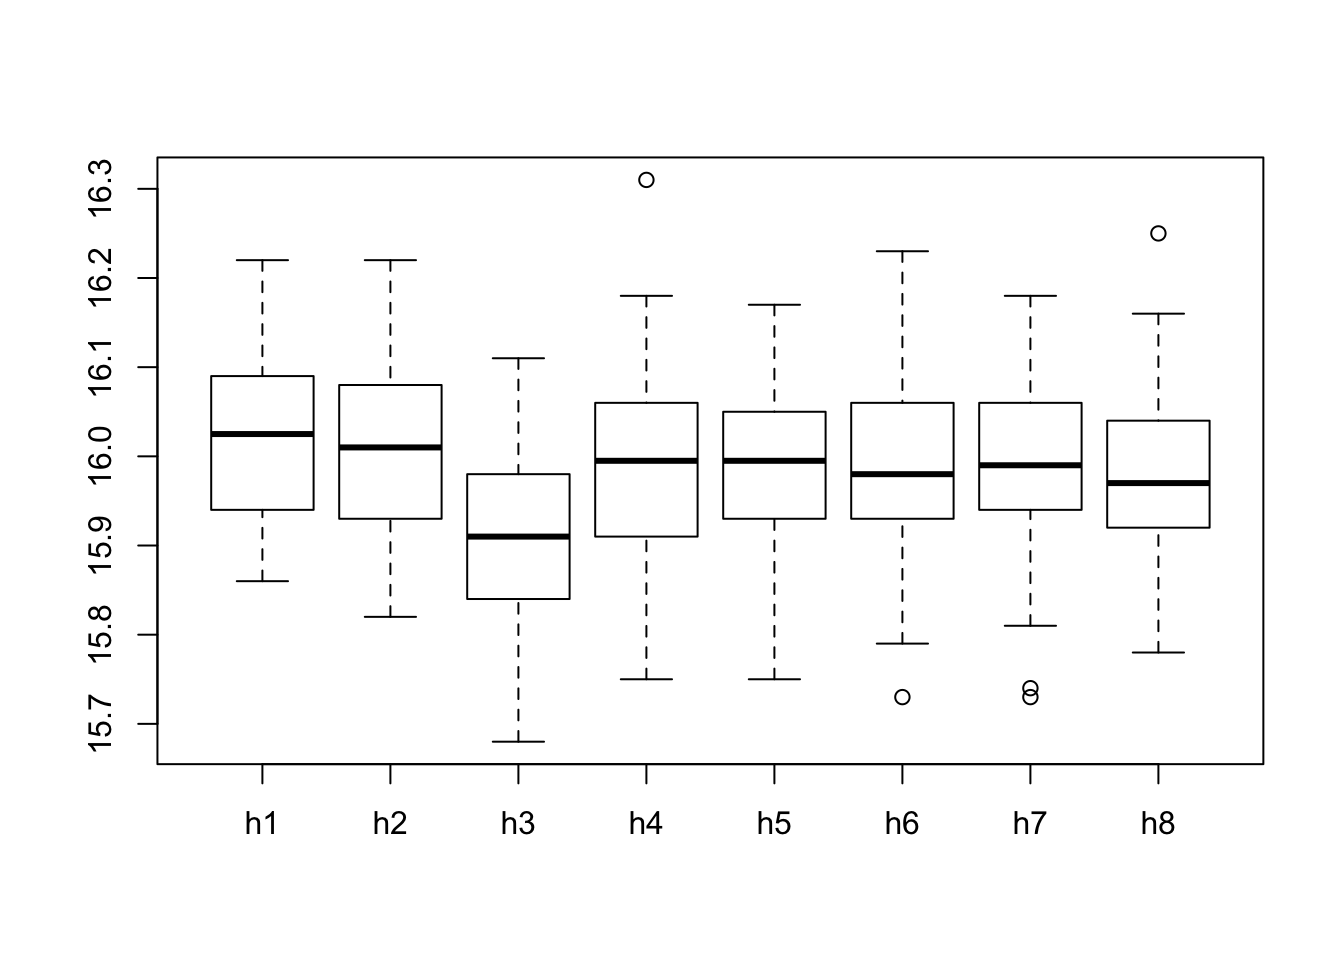
\includegraphics[width=0.6\linewidth]{statthink_files/figure-latex/unnamed-chunk-128-1} \end{center}

Examining the plots we may see that evidence for the existence of
outliers can be spotted on the 4th, 6th, 7th, and 8th hours, providing
an answer to Question~4.5

\hypertarget{example-5}{%
\subsection{Example 5}\label{example-5}}

A measurement follows the \(\mbox{Uniform}(0,b)\), for an unknown value of
\(b\). Two statisticians propose two distinct ways to estimate the unknown
quantity \(b\) with the aid of a sample of size \(n=100\). Statistician A
proposes to use twice the sample average (\(2 \bar X\)) as an estimate.
Statistician B proposes to use the largest observation instead.

The motivation for the proposal made by Statistician A is that the
expectation of the measurement is equal to \(\Expec(X) = b/2\). A
reasonable way to estimate the expectation is to use the sample average
\(\bar X\). Thereby, a reasonable way to estimate \(b\), twice the
expectation, is to use \(2 \bar X\). A motivation for the proposal made by
Statistician B is that although the largest observation is indeed
smaller that \(b\), still it may not be much smaller than that value.

In order to choose between the two options they agreed to prefer the
statistic that tends to have values that are closer to \(b\). (with
respect to the sampling distribution). They also agreed to compute the
expectation and variance of each statistic. The performance of a
statistic is evaluated using the \emph{mean square error} (MSE), which is
defined as the sum of the variance and the squared difference between
the expectation and \(b\). Namely, if \(T\) is the statistic (either the one
proposed by Statistician A or Statistician B) then

\[MSE = \Var(T) + (\Expec(T) - b)^2\;.\] A smaller mean square error
corresponds to a better, more accurate, statistic.

\begin{enumerate}
\def\labelenumi{\arabic{enumi}.}
\item
  Assume that the actual value of \(b\) is 10 (\(b=10\)). Use simulations
  to compute the expectation, the variance and the MSE of the
  statistic proposed by Statistician A.
\item
  Assume that the actual value of \(b\) is 10 (\(b=10\)). Use simulations
  to compute the expectation, the variance and the MSE of the
  statistic proposed by Statistician B. (Hint: the maximal value of a
  sequence can be computed with the function ``\texttt{max}''.)
\item
  Assume that the actual value of \(b\) is 13.7 (\(b=13.7\)). Use
  simulations to compute the expectation, the variance and the MSE of
  the statistic proposed by Statistician A.
\item
  Assume that the actual value of \(b\) is 13.7 (\(b=13.7\)). Use
  simulations to compute the expectation, the variance and the MSE of
  the statistic proposed by Statistician B. (Hint: the maximal value
  of a sequence can be computed with the function ``\texttt{max}''.)
\item
  Based on the results in Questions~5.1--4, which of the two statistics
  seems to be preferable?
\end{enumerate}

\hypertarget{solution-4}{%
\subsection*{Solution}\label{solution-4}}


In Questions 5.1 and 5.2 we take the value of \(b\) to be equal to 10.
Consequently, the distribution of a measurement is
\(\mbox{Uniform}(0,10)\). In order to generate the sampling distributions
we produce two sequences, ``\texttt{A}'' and ``\texttt{B}'', both of length 100,000, with
the evaluations of the statistics:

\begin{Shaded}
\begin{Highlighting}[]
\NormalTok{A <-}\StringTok{ }\KeywordTok{rep}\NormalTok{(}\DecValTok{0}\NormalTok{,}\DecValTok{10}\OperatorTok{^}\DecValTok{5}\NormalTok{)}
\NormalTok{B <-}\StringTok{ }\KeywordTok{rep}\NormalTok{(}\DecValTok{0}\NormalTok{,}\DecValTok{10}\OperatorTok{^}\DecValTok{5}\NormalTok{)}
\ControlFlowTok{for}\NormalTok{(i }\ControlFlowTok{in} \DecValTok{1}\OperatorTok{:}\DecValTok{10}\OperatorTok{^}\DecValTok{5}\NormalTok{) \{}
\NormalTok{  X.samp <-}\StringTok{ }\KeywordTok{runif}\NormalTok{(}\DecValTok{100}\NormalTok{,}\DecValTok{0}\NormalTok{,}\DecValTok{10}\NormalTok{)}
\NormalTok{  A[i] <-}\StringTok{ }\DecValTok{2}\OperatorTok{*}\KeywordTok{mean}\NormalTok{(X.samp)}
\NormalTok{  B[i] <-}\StringTok{ }\KeywordTok{max}\NormalTok{(X.samp)}
\NormalTok{\}}
\end{Highlighting}
\end{Shaded}

Observe that in each iteration of the ``\texttt{for}'' loop a sample of size
\(n=100\) from the \(\mbox{Uniform}(0,10)\) distribution is generated. The
statistic proposed by Statistician A (``\texttt{2*mean(X.samp)}'') is computed
and stored in sequence ``\texttt{A}'' and the statistic proposed by Statistician
B (``\texttt{max(X.samp)}'') is computed and stored in sequence ``\texttt{B}''.

Consider the statistic proposed by Statistician A:

\begin{Shaded}
\begin{Highlighting}[]
\KeywordTok{mean}\NormalTok{(A)}
\end{Highlighting}
\end{Shaded}

\begin{verbatim}
## [1] 9.9993879
\end{verbatim}

\begin{Shaded}
\begin{Highlighting}[]
\KeywordTok{var}\NormalTok{(A)}
\end{Highlighting}
\end{Shaded}

\begin{verbatim}
## [1] 0.33317939
\end{verbatim}

\begin{Shaded}
\begin{Highlighting}[]
\KeywordTok{var}\NormalTok{(A) }\OperatorTok{+}\StringTok{ }\NormalTok{(}\KeywordTok{mean}\NormalTok{(A)}\OperatorTok{-}\DecValTok{10}\NormalTok{)}\OperatorTok{^}\DecValTok{2}
\end{Highlighting}
\end{Shaded}

\begin{verbatim}
## [1] 0.33317976
\end{verbatim}

The expectation of the statistic is 9.99772 and the variance is
0.3341673. Consequently, we get that the mean square error is equal to

\[0.3341673 + (9.99772 - 10)^2 = 0.3341725\;.\]

Next, deal with the statistic proposed by Statistician B:

\begin{Shaded}
\begin{Highlighting}[]
\KeywordTok{mean}\NormalTok{(B)}
\end{Highlighting}
\end{Shaded}

\begin{verbatim}
## [1] 9.9004284
\end{verbatim}

\begin{Shaded}
\begin{Highlighting}[]
\KeywordTok{var}\NormalTok{(B)}
\end{Highlighting}
\end{Shaded}

\begin{verbatim}
## [1] 0.0097122034
\end{verbatim}

\begin{Shaded}
\begin{Highlighting}[]
\KeywordTok{var}\NormalTok{(B) }\OperatorTok{+}\StringTok{ }\NormalTok{(}\KeywordTok{mean}\NormalTok{(B)}\OperatorTok{-}\DecValTok{10}\NormalTok{)}\OperatorTok{^}\DecValTok{2}
\end{Highlighting}
\end{Shaded}

\begin{verbatim}
## [1] 0.019626717
\end{verbatim}

The expectation of the statistic is 9.901259 and the variance is
0.00950006. Consequently, we get that the mean square error is equal to

\[0.00950006 + (9.901259 - 10)^2 = 0.01924989\;.\] Observe that the mean
square error of the statistic proposed by Statistician B is smaller.

For Questions~5.3 and 5.4 we run the same type of simulations. All we
change is the value of \(b\) (from 10 to 13.7):

\begin{Shaded}
\begin{Highlighting}[]
\NormalTok{A <-}\StringTok{ }\KeywordTok{rep}\NormalTok{(}\DecValTok{0}\NormalTok{,}\DecValTok{10}\OperatorTok{^}\DecValTok{5}\NormalTok{)}
\NormalTok{B <-}\StringTok{ }\KeywordTok{rep}\NormalTok{(}\DecValTok{0}\NormalTok{,}\DecValTok{10}\OperatorTok{^}\DecValTok{5}\NormalTok{)}
\ControlFlowTok{for}\NormalTok{(i }\ControlFlowTok{in} \DecValTok{1}\OperatorTok{:}\DecValTok{10}\OperatorTok{^}\DecValTok{5}\NormalTok{) \{}
\NormalTok{  X.samp <-}\StringTok{ }\KeywordTok{runif}\NormalTok{(}\DecValTok{100}\NormalTok{,}\DecValTok{0}\NormalTok{,}\FloatTok{13.7}\NormalTok{)}
\NormalTok{  A[i] <-}\StringTok{ }\DecValTok{2}\OperatorTok{*}\KeywordTok{mean}\NormalTok{(X.samp)}
\NormalTok{  B[i] <-}\StringTok{ }\KeywordTok{max}\NormalTok{(X.samp)}
\NormalTok{\}}
\end{Highlighting}
\end{Shaded}

Again, considering the statistic proposed by Statistician A we get:

\begin{Shaded}
\begin{Highlighting}[]
\KeywordTok{mean}\NormalTok{(A)}
\end{Highlighting}
\end{Shaded}

\begin{verbatim}
## [1] 13.698413
\end{verbatim}

\begin{Shaded}
\begin{Highlighting}[]
\KeywordTok{var}\NormalTok{(A)}
\end{Highlighting}
\end{Shaded}

\begin{verbatim}
## [1] 0.62967999
\end{verbatim}

\begin{Shaded}
\begin{Highlighting}[]
\KeywordTok{var}\NormalTok{(A) }\OperatorTok{+}\StringTok{ }\NormalTok{(}\KeywordTok{mean}\NormalTok{(A)}\OperatorTok{-}\FloatTok{13.7}\NormalTok{)}\OperatorTok{^}\DecValTok{2}
\end{Highlighting}
\end{Shaded}

\begin{verbatim}
## [1] 0.62968251
\end{verbatim}

The expectation of the statistic in this setting is 13.70009 and the
variance is 0.6264204. Consequently, we get that the mean square error
is equal to

\[0.6264204 + (13.70009 - 13.7)^2 = 0.6264204\;.\]

For the statistic proposed by Statistician B we obtain:

\begin{Shaded}
\begin{Highlighting}[]
\KeywordTok{mean}\NormalTok{(B)}
\end{Highlighting}
\end{Shaded}

\begin{verbatim}
## [1] 13.564837
\end{verbatim}

\begin{Shaded}
\begin{Highlighting}[]
\KeywordTok{var}\NormalTok{(B)}
\end{Highlighting}
\end{Shaded}

\begin{verbatim}
## [1] 0.018034803
\end{verbatim}

\begin{Shaded}
\begin{Highlighting}[]
\KeywordTok{var}\NormalTok{(B) }\OperatorTok{+}\StringTok{ }\NormalTok{(}\KeywordTok{mean}\NormalTok{(B)}\OperatorTok{-}\FloatTok{13.7}\NormalTok{)}\OperatorTok{^}\DecValTok{2}
\end{Highlighting}
\end{Shaded}

\begin{verbatim}
## [1] 0.036303871
\end{verbatim}

The expectation of the statistic is 13.56467 and the variance is
0.01787562. Consequently, we get that the mean square error is equal to

\[0.01787562 + (13.56467 - 13.7)^2 = 0.03618937\;.\] Once more, the mean
square error of the statistic proposed by Statistician B is smaller.

Considering the fact that the mean square error of the statistic
proposed by Statistician B is smaller in both cases we may conclude that
this statistic seems to be better for estimation of \(b\) in this setting
of Uniformly distributed measurements\footnote{As a matter of fact, it can be proved that the statistic proposed
  by Statistician B has a smaller mean square error than the statistic
  proposed by Statistician A, for \emph{any} value of \(b\)}.

\hypertarget{discussion-in-the-forum}{%
\subsection*{Discussion in the Forum}\label{discussion-in-the-forum}}


In this course we have learned many subjects. Most of these subjects,
especially for those that had no previous exposure to statistics, were
unfamiliar. In this forum we would like to ask you to share with us the
difficulties that you encountered.

What was the topic that was most difficult for you to grasp? In your
opinion, what was the source of the difficulty?

When forming your answer to this question we will appreciate if you
could elaborate and give details of what the problem was. Pointing to
deficiencies in the learning material and confusing explanations will
help us improve the presentation for the future application of this
course.

\hypertarget{ChapInference}{%
\chapter{Introduction to Statistical Inference}\label{ChapInference}}

\hypertarget{student-learning-objectives-3}{%
\section{Student Learning Objectives}\label{student-learning-objectives-3}}

The next section of this chapter introduces the basic issues and tools
of statistical inference. These tools are the subject matter of the
second part of this book. In Chapters~\ref{ChapInference}--\ref{ChapLogistic}
we use data on the specifications of cars in order to demonstrate the
application of the tools for making statistical inference. In the third
section of this chapter we present the data frame that contains this
data. The fourth section reviews probability topics that were discussed
in the first part of the book and are relevant for the second part. By
the end of this chapter, the student should be able to:

\begin{itemize}
\item
  Define key terms that are associated with inferential statistics.
\item
  Recognize the variables of the ``\texttt{cars.csv}'' data frame.
\item
  Revise concepts related to random variables, the sampling
  distribution and the Central Limit Theorem.
\end{itemize}

\hypertarget{key-terms-1}{%
\section{Key Terms}\label{key-terms-1}}

The first part of the book deals with descriptive statistics and with
probability. In descriptive statistics one investigates the
characteristics of the data by using graphical tools and numerical
summaries. The frame of reference is the observed data. In probability,
on the other hand, one extends the frame of reference to include all
data sets that could have potentially emerged, with the observed data as
one among many.

The second part of the book deals with inferential statistics. The aim
of statistical inference is to gain insight regarding the population
parameters from the observed data. The method for obtaining such insight
involves the application of formal computations to the data. The
interpretation of the outcome of these formal computations is carried
out in the probabilistic context, in which one considers the application
of these formal computations to all potential data sets. The
justification for using the specific form of computation on the observed
data stems from the examination of the probabilistic properties of the
formal computations.

Typically, the formal computations will involve statistics, which are
functions of the data. The assessment of the probabilistic properties of
the computations will result from the sampling distribution of these
statistics.

An example of a problem that requires statistical inference is the
estimation of a parameter of the population using the observed data.
\emph{Point estimation} attempts to obtain the best guess to the value of
that parameter. An \emph{estimator} is a statistic that produces such a
guess. One may prefer an estimator whose sampling distribution is more
concentrated about the population parameter value over another estimator
whose sampling distribution is less so. Hence, the justification for
selecting a specific statistic as an estimator is a consequence of the
probabilistic characteristics of this statistic in the context of the
sampling distribution.

For example, a car manufacture may be interested in the fuel consumption
of a new type of car. In order to do so the manufacturer may apply a
standard test cycle to a sample of 10 new cars of the given type and
measure their fuel consumptions. The parameter of interest is the
average fuel consumption among \emph{all} cars of the given type. The average
consumption of the 10 cars is a point estimate of the parameter of
interest.

An alternative approach for the estimation of a parameter is to
construct an interval that is most likely to contain the population
parameter. Such an interval, which is computed on the basis of the data,
is called the a \emph{confidence interval}. The sampling probability that the
confidence interval will indeed contain the parameter value is called
the \emph{confidence level}. Confidence intervals are constructed so as to
have a prescribed confidence level.

A different problem in statistical inference is \emph{hypothesis testing}.
The scientific paradigm involves the proposal of new theories and
hypothesis that presumably provide a better description for the laws of
Nature. On the basis of these hypothesis one may propose predictions
that can be examined empirically. If the empirical evidence is
consistent with the predictions of the new hypothesis but not with those
of the old theory then the old theory is rejected in favor of the new
one. Otherwise, the established theory maintains its status. Statistical
hypothesis testing is a formal method for determining which of the two
hypothesis should prevail that uses this paradigm.

Each of the two hypothesis, the old and the new, predicts a different
distribution for the empirical measurements. In order to decide which of
the distributions is more in tune with the data a statistic is computed.
This statistic is called the \emph{test statistic}. A threshold is set and,
depending on where the test statistic falls with respect to this
threshold, the decision is made whether or not to reject the old theory
in favor of the new one.

This decision rule is not error proof, since the test statistic may fall
by chance on the wrong side of the threshold. Nonetheless, by the
examination of the sampling distribution of the test statistic one is
able to assess the probability of making an error. In particular, the
probability of erroneously rejecting the currently accepted theory (the
old one) is called the \emph{significance level} of the test. Indeed, the
threshold is selected in order to assure a small enough significance
level.

Returning to the car manufacturer. Assume that the car in question is
manufactured in two different factories. One may want to examine the
hypothesis that the car's fuel consumption is the same for both
factories. If 5 of the tested cars were manufactured in one factory and
the other 5 in the other factory then the test may be based on the
absolute value of the difference between the average consumption of the
first 5 and the average consumption of the other 5.

The method of testing hypothesis is also applied in other practical
settings where it is required to make decisions. For example, before a
new treatment to a medical condition is approved for marketing by the
appropriate authorities it must undergo a process of objective testing
through clinical trials. In these trials the new treatment is
administered to some patients while other obtain the (currently)
standard treatment. Statistical tests are applied in order to compare
the two groups of patient. The new treatment is released to the market
only if it is shown to be beneficial with statistical significance and
it is shown to have no unacceptable side effects.

In subsequent chapters we will discuss in more details the computation
of point estimation, the construction of confidence intervals, and the
application of hypothesis testing. The discussion will be initiated in
the context of a single measurement but will later be extended to
settings that involve comparison of measurements.

An example of such analysis is the analysis of clinical trials where the
response of the patients treated with the new procedure is compared to
the response of patients that were treated with the conventional
treatment. This comparison involves the same measurement taken for two
sub-samples. The tools of statistical inference -- hypothesis testing,
point estimation and the construction of confidence intervals -- may be
used in order to carry out this comparison.

Other comparisons may involve two measurements taken for the entire
sample. An important tool for the investigation of the relations between
two measurements, or variables, is \emph{regression}. Models of regression
describe the change in the distribution in one variable as a function of
the other variable. Again, point estimation, confidence intervals, and
hypothesis testing can be carried out in order to examine regression
models. The variable whose distribution is the target of investigation
is called the response. The other variable that may affect that
distribution is called the explanatory variable.

\hypertarget{the-cars-data-set}{%
\section{The Cars Data Set}\label{the-cars-data-set}}

Statistical inference is applied to data in order to address specific
research question. We will demonstrate different inferential procedures
using a specific data set with the aim of making the discussion of the
different procedures more concrete. The same data set will be used for
all procedures that are presented in
Chapters~\ref{ChapEstimation}--\ref{ChapLogistic}\footnote{Other data sets will be used in Chapter~\[ch:CaseStudies\] and in
  the quizzes and assignments.}. This data set contains
information on various models of cars and is stored in the CVS file
``\texttt{cars.csv}''\footnote{The original ``Automobiles'' data set is accessible at the UCI
  Machine Learning Repository (\url{http://archive.ics.uci.edu/ml}). This
  data was assembled by Jeffrey C. Schlimmer, using as source the 1985
  Model Import Car and Truck Specifications, 1985 Ward's Automotive
  Yearbook. The current file ``\texttt{cars.csv}'' is based on all 205
  observations of the original data set. We selected 17 of the 26
  variables available in the original source.}. The file can be found on the internet at
\url{http://pluto.huji.ac.il/~msby/StatThink/Datasets/cars.csv}. You are
advised to download this file to your computer and store it in the
working directory of \texttt{R}.

Let us read the content of the CSV file into an \texttt{R} data frame and
produce a brief summary:

\begin{Shaded}
\begin{Highlighting}[]
\NormalTok{cars <-}\StringTok{ }\KeywordTok{read.csv}\NormalTok{(}\StringTok{"_data/cars.csv"}\NormalTok{)}
\KeywordTok{summary}\NormalTok{(cars)}
\end{Highlighting}
\end{Shaded}

\begin{verbatim}
##          make      fuel.type   num.of.doors       body.style drive.wheels
##  toyota    : 32   diesel: 20   four:114     convertible: 6   4wd:  9     
##  nissan    : 18   gas   :185   two : 89     hardtop    : 8   fwd:120     
##  mazda     : 17                NA's:  2     hatchback  :70   rwd: 76     
##  honda     : 13                             sedan      :96               
##  mitsubishi: 13                             wagon      :25               
##  subaru    : 12                                                          
##  (Other)   :100                                                          
##  engine.location   wheel.base          length           width       
##  front:202       Min.   : 86.600   Min.   :141.10   Min.   :60.300  
##  rear :  3       1st Qu.: 94.500   1st Qu.:166.30   1st Qu.:64.100  
##                  Median : 97.000   Median :173.20   Median :65.500  
##                  Mean   : 98.757   Mean   :174.05   Mean   :65.908  
##                  3rd Qu.:102.400   3rd Qu.:183.10   3rd Qu.:66.900  
##                  Max.   :120.900   Max.   :208.10   Max.   :72.300  
##                                                                     
##      height        curb.weight      engine.size       horsepower    
##  Min.   :47.800   Min.   :1488.0   Min.   : 61.00   Min.   : 48.00  
##  1st Qu.:52.000   1st Qu.:2145.0   1st Qu.: 97.00   1st Qu.: 70.00  
##  Median :54.100   Median :2414.0   Median :120.00   Median : 95.00  
##  Mean   :53.725   Mean   :2555.6   Mean   :126.91   Mean   :104.26  
##  3rd Qu.:55.500   3rd Qu.:2935.0   3rd Qu.:141.00   3rd Qu.:116.00  
##  Max.   :59.800   Max.   :4066.0   Max.   :326.00   Max.   :288.00  
##                                                     NA's   :2       
##     peak.rpm         city.mpg      highway.mpg         price      
##  Min.   :4150.0   Min.   :13.00   Min.   :16.000   Min.   : 5118  
##  1st Qu.:4800.0   1st Qu.:19.00   1st Qu.:25.000   1st Qu.: 7775  
##  Median :5200.0   Median :24.00   Median :30.000   Median :10295  
##  Mean   :5125.4   Mean   :25.22   Mean   :30.751   Mean   :13207  
##  3rd Qu.:5500.0   3rd Qu.:30.00   3rd Qu.:34.000   3rd Qu.:16500  
##  Max.   :6600.0   Max.   :49.00   Max.   :54.000   Max.   :45400  
##  NA's   :2                                         NA's   :4
\end{verbatim}

Observe that the first 6 variables are factors, i.e.~they contain
qualitative data that is associated with categorization or the
description of an attribute. The last 11 variable are numeric and
contain quantitative data.

Factors are summarized in \texttt{R} by listing the attributes and the
frequency of each attribute value. If the number of attributes is large
then only the most frequent attributes are listed. Numerical variables
are summarized in \texttt{R} with the aid of the smallest and largest values,
the three quartiles (Q1, the median, and Q3) and the average (mean).

The third factor variable, ``\texttt{num.of.doors}'', as well as several of the
numerical variables have a special category titled ``\texttt{NA’s}''. This
category describes the number of missing values among the observations.
For a given variable, the observations for which a value for the
variable is not recorded, are marked as missing. \texttt{R} uses the symbol
``\texttt{NA}'' to identify a missing value\footnote{Indeed, if you scan the CSV file directly by opening it with a
  spreadsheet then every now and again you will encounter this symbol.}.

Missing observations are a concern in the analysis of statistical data.
If the relative frequency of missing values is substantial and the
reason for not obtaining the data for specific observations is related
to the phenomena under investigation than naïve statistical inference
may produce biased conclusions. In the ``\texttt{cars}'' data frame missing
values are less of a concern since their relative frequency is low.

One should be on the lookout for missing values when applying \texttt{R} to
data since the different functions may have different ways for dealing
with missing values. One should make sure that the appropriate way is
applied for the specific analysis.

Consider the variables of the data frame ``\texttt{cars}'':

\begin{description}
\item[\texttt{make}:]
The name of the car producer (a factor).
\item[\texttt{fuel.type}:]
The type of fuel used by the car, either diesel or gas (a factor).
\item[\texttt{num.of.doors}:]
The number of passenger doors, either two or four (a factor).
\item[\texttt{body.style}:]
The type of the car (a factor).
\item[\texttt{drive.wheels}:]
The wheels powered by the engine (a factor).
\item[\texttt{engine.location}:]
The location in the car of the engine (a factor).
\item[\texttt{wheel.base}:]
The distance between the centers of the front and rear wheels in
inches (numeric).
\item[\texttt{length}:]
The length of the body of the car in inches (numeric).
\item[\texttt{width}:]
The width of the body of the car in inches (numeric).
\item[\texttt{height}:]
The height of the car in inches (numeric).
\item[\texttt{curb.weight}:]
The total weight in pounds of a vehicle with standard equipment and
a full tank of fuel, but with no passengers or cargo (numeric).
\item[\texttt{engine.size}:]
The volume swept by all the pistons inside the cylinders in cubic
inches (numeric).
\item[\texttt{horsepower}:]
The power of the engine in horsepowers (numeric).
\item[\texttt{peak.rpm}:]
The top speed of the engine in rounds-per-minute (numeric).
\item[\texttt{city.mpg}:]
The fuel consumption of the car in city driving conditions, measured
as miles per gallon of fuel (numeric).
\item[\texttt{highway.mpg}:]
The fuel consumption of the car in highway driving conditions,
measured as miles per gallon of fuel (numeric).
\item[\texttt{price}:]
The retail price of the car in US Dollars (numeric).
\end{description}

\hypertarget{the-sampling-distribution-1}{%
\section{The Sampling Distribution}\label{the-sampling-distribution-1}}

\hypertarget{statistics-1}{%
\subsection{Statistics}\label{statistics-1}}

Statistical inferences, be it point estimation, confidence intervals, or
testing hypothesis, are based on statistics computed from the data.
Examples of statistics are the sample average and the sample standard
deviation. These are important examples, but clearly not the only ones.
Given numerical data, one may compute the smallest value, the largest
value, the quartiles, and the median. All are examples of statistics.
Statistics may also be associated with factors. The frequency of a given
attribute among the observations is a statistic. (An example of such
statistic is the frequency of diesel cars in the data frame.) As part of
the discussion in the subsequent chapters we will consider these and
other types of statistics.

Any statistic, when computed in the context of the data frame being
analyzed, obtains a single numerical value. However, once a sampling
distribution is being considered then one may view the same statistic as
a random variable. A statistic is a function or a formula which is
applied to the data frame. Consequently, when a random collection of
data frames is the frame of reference then the application of the
formula to each of the data frames produces a random collection of
values, which is the sampling distribution of the statistic.

We distinguish in the text between the case where the statistic is
computed in the context of the given data frame and the case where the
computation is conducted in the context of the random sample. This
distinguishing is emphasized by the use of small letters for the former
and capital letters for the later. Consider, for example, the sample
average. In the context of the observed data we denote the data values
for a specific variable by \(x_1, x_2, \ldots, x_n\). The sample average
computed for these values is denoted by

\[\bar x = \frac{x_1 + x_2 + \cdots + x_n}{n}\;.\] On the other hand, if
the discussion of the sample average is conducted in the context of a
random sample then the sample is a sequence \(X_1, X_2, \ldots, X_n\) of
random variables. The sample average is denoted in this context as

\[\bar X = \frac{X_1 + X_2 + \cdots + X_n}{n}\;.\] The same formula that
was applied to the data values is applied now to the random components
of the random sample. In the first context \(\bar x\) is an observed
non-random quantity. In the second context \(\bar X\) is a random
variable, an abstract mathematical concept.

A second example is the sample variance. When we compute the sample
variance for the observed data we use the formula:

\[s^2 = \frac{\mbox{Sum of the squares of the deviations}}{\mbox{Number of values in the sample}-1}= \frac{\sum_{i=1}^n (x_i - \bar x)^2}{n-1}\;.\]
However, when we discuss the sampling distribution of the sample
variance we apply the same formula to the random sample:

\[S^2 = \frac{\mbox{Sum of the squares of the deviations}}{\mbox{Number of values in the sample}-1}= \frac{\sum_{i=1}^n (X_i - \bar X)^2}{n-1}\;.\]
Again, \(S^2\) is a random variable whereas \(s^2\) is a non-random
quantity: The evaluation of the random variable at the specific sample
that is being observed.

\hypertarget{the-sampling-distribution-2}{%
\subsection{The Sampling Distribution}\label{the-sampling-distribution-2}}

The sampling distribution may emerge as random selection of samples from
a particular population. In such a case, the sampling distribution of
the sample, and hence of the statistic, is linked to the distribution of
values of the variable in the population.

Alternatively, one may assign theoretical distribution to the
measurement associated with the variable. In this other case the
sampling distribution of the statistic is linked to the theoretical
model.

Consider, for example, the variable ``\texttt{price}'' that describes the prices
of the 205 car types (with 4 prices missing) in the data frame ``\texttt{cars}''.
In order to define a sampling distribution one may imagine a larger
population of car types, perhaps all the car types that were sold during
the 80's in the United States, or some other frame of reference, with
the car types that are included in the data frame considered as a random
sample from that larger population. The observed sample corresponds to
car types that where sold in 1985. Had one chosen to consider car types
from a different year then one may expect to obtain other evaluations of
the price variable. The reference population, in this case, is the
distribution of the prices of the car types that were sold during the
80's and the sampling distribution is associated with a random selection
of a particular year within this period and the consideration of prices
of car types sold in that year. The data for 1985 is what we have at
hand. But in the sampling distribution we take into account the
possibility that we could have obtained data for 1987, for example,
rather than the data we did get.

An alternative approach for addressing sampling distribution is to
consider a theoretical model. Referring again to the variable ``\texttt{price}''
one may propose an Exponential model for the distribution of the prices
of cars. This model implies that car types in the lower spectrum of the
price range are more frequent than cars with a higher price tag. With
this model in mind, one may propose the sampling distribution to be
composed of 205 unrelated copies from the Exponential distribution (or
201 if we do not want to include the missing values). The rate \(\lambda\)
of the associated Exponential distribution is treated as an unknown
parameter. One of the roles of statistical inference is to estimate the
value of this parameter with the aid of the data at hand.

Sampling distribution is relevant also for factor variables. Consider
the variable ``\texttt{fuel.type}'' as an example. In the given data frame the
frequency of diesel cars is 20. However, had one considered another year
during the 80's one may have obtained a different frequency, resulting
in a sampling distribution. This type of sampling distribution refers to
all cars types that were sold in the United States during the 80's as
the frame of reference.

Alternatively, one may propose a theoretical model for the sampling
distribution. Imagine there is a probability \(p\) that a car runs on
diesel (and probability \(1-p\) that it runs on gas). Hence, when one
selects 205 car types at random then one obtains that the distribution
of the frequency of car types that run on diesel has the
\(\mathrm{Binomial}(205,p)\) distribution. This is the sampling
distribution of the frequency statistic. Again, the value of \(p\) is
unknown and one of our tasks is to estimate it from the data we observe.

In the context of statistical inference the use of theoretical models
for the sampling distribution is the standard approach. There are
situation, such as the application surveys to a specific target
population, where the consideration of the entire population as the
frame of reference is more natural. But, in most other applications the
consideration of theoretical models is the method of choice. In this
part of the book, where we consider statistical inference, we will
always use the theoretical approach for modeling the sampling
distribution.

\hypertarget{theoretical-distributions-of-observations}{%
\subsection{Theoretical Distributions of Observations}\label{theoretical-distributions-of-observations}}

In the first part of the book we introduced several theoretical models
that may describe the distribution of an observation. Let us take the
opportunity and review the list of models:

\begin{description}
\item[Binomial:]
The Binomial distribution is used in settings that involve counting
the number of occurrences of a particular outcome. The parameters
that determine the distribution are \(n\), the number of observations,
and \(p\), the probability of obtaining the particular outcome in each
observation. The expression ``\(\mathrm{Binomial}(n,p)\)'' is used to
mark the Binomial distribution. The sample space for this
distribution is formed by the integer values
\(\{0, 1, 2, \ldots, n\}\). The expectation of the distribution is
\(np\) and the variance is \(np(1-p)\). The functions ``\texttt{dbinom}'',
``\texttt{pbinom}'', and ``\texttt{qbinom}'' may be used in order to compute the
probability, the cumulative probability, and the percentiles,
respectively, for the Binomial distribution. The function ``\texttt{rbinom}''
can be used in order to simulate a random sample from this
distribution.
\item[Poisson:]
The Poisson distribution is also used in settings that involve
counting. This distribution approximates the Binomial distribution
when the number of examinations \(n\) is large but the probability \(p\)
of the particular outcome is small. The parameter that determines
the distribution is the expectation \(\lambda\). The expression
``\(\mathrm{Poisson}(\lambda)\)'' is used to mark the Poisson
distribution. The sample space for this distribution is the entire
collection of natural numbers \(\{0, 1, 2, \ldots\}\). The expectation
of the distribution is \(\lambda\) and the variance is also \(\lambda\).
The functions ``\texttt{dpois}'', ``\texttt{ppois}'', and ``\texttt{qpois}'' may be used in
order to compute the probability, the cumulative probability, and
the percentiles, respectively, for the Poisson distribution. The
function ``\texttt{rpois}'' can be used in order to simulate a random sample
from this distribution.
\item[Uniform:]
The Uniform distribution is used in order to model measurements that
may have values in a given interval, with all values in this
interval equally likely to occur. The parameters that determine the
distribution are \(a\) and \(b\), the two end points of the interval.
The expression ``\(\mathrm{Uniform}(a,b)\)'' is used to identify the
Uniform distribution. The sample space for this distribution is the
interval \([a,b]\). The expectation of the distribution is \((a+b)/2\)
and the variance is \((b-a)^2/12\). The functions ``\texttt{dunif}'',
``\texttt{punif}'', and ``\texttt{qunif}'' may be used in order to compute the
density, the cumulative probability, and the percentiles for the
Uniform distribution. The function ``\texttt{runif}'' can be used in order to
simulate a random sample from this distribution.
\item[Exponential:]
The Exponential distribution is frequently used to model times
between events. It can also be used in other cases where the outcome
of the measurement is a positive number and where a smaller value is
more likely than a larger value. The parameter that determines the
distribution is the rate \(\lambda\). The expression
``\(\mathrm{Exponential}(\lambda)\)'' is used to identify the
Exponential distribution. The sample space for this distribution is
the collection of positive numbers. The expectation of the
distribution is \(1/\lambda\) and the variance is \(1/\lambda^2\). The
functions ``\texttt{dexp}'', ``\texttt{pexp}'', and ``\texttt{qexp}'' may be used in order to
compute the density, the cumulative probability, and the
percentiles, respectively, for the Exponential distribution. The
function ``\texttt{rexp}'' can be used in order to simulate a random sample
from this distribution.
\item[Normal:]
The Normal distribution frequently serves as a generic model for the
distribution of a measurement. Typically, it also emerges as an
approximation of the sampling distribution of statistics. The
parameters that determine the distribution are the expectation \(\mu\)
and the variance \(\sigma^2\). The expression
``\(\mathrm{Normal}(\mu,\sigma^2)\)'' is used to mark the Normal
distribution. The sample space for this distribution is the
collection of all numbers, negative or positive. The expectation of
the distribution is \(\mu\) and the variance is \(\sigma^2\). The
functions ``\texttt{dnorm}'', ``\texttt{pnorm}'', and ``\texttt{qnorm}'' may be used in order
to compute the density, the cumulative probability, and the
percentiles for the Normal distribution. The function ``\texttt{rnorm}'' can
be used in order to simulate a random sample from this distribution.
\end{description}

\hypertarget{sampling-distribution-of-statistics}{%
\subsection{Sampling Distribution of Statistics}\label{sampling-distribution-of-statistics}}

Theoretical models describe the distribution of a measurement as a
function of a parameter, or a small number of parameters. For example,
in the Binomial case the distribution is determined by the number of
trials \(n\) and by the probability of success in each trial \(p\). In the
Poisson case the distribution is a function of the expectation
\(\lambda\). For the Uniform distribution we may use the end-points of the
interval, \(a\) and \(b\), as the parameters. In the Exponential case, the
rate \(\lambda\) is a natural parameter for specifying the distribution
and in Normal case the expectation \(\mu\) and the variance \(\sigma^2\) my
be used for that role.

The general formulation of statistical inference problems involves the
identification of a theoretical model for the distribution of the
measurements. This theoretical model is a function of a parameter whose
value is unknown. The goal is to produce statements that refer to this
unknown parameter. These statements are based on a sample of
observations from the given distribution.

For example, one may try to guess the value of the parameter (point
estimation), one may propose an interval which contains the value of the
parameter with some subscribed probability (confidence interval) or one
may test the hypothesis that the parameter obtains a specific value
(hypothesis testing).

The vehicles for conducting the statistical inferences are statistics
that are computed as a function of the measurements. In the case of
point estimation these statistics are called \emph{estimators}. In the case
where the construction of an interval that contains the value of the
parameter is the goal then the statistics are called \emph{confidence
interval}. In the case of testing hypothesis these statistics are called
\emph{test statistics}.

In all cases of inference, The relevant statistic possesses a
distribution that it inherits from the sampling distribution of the
observations. This distribution is the sampling distribution of the
statistic. The properties of the statistic as a tool for inference are
assessed in terms of its sampling distribution. The sampling
distribution of a statistic is a function of the sample size and of the
parameters that determine the distribution of the measurements, but
otherwise may be of complex structure.

In order to assess the performance of the statistics as agents of
inference one should be able to determine their sampling distribution.
We will apply two approaches for this determination. One approach is to
use a Normal approximation. This approach relies on the Central Limit
Theorem. The other approach is to simulate the distribution. This other
approach relies on the functions available in \texttt{R} for the simulation of
a random sample from a given distribution.

\hypertarget{the-normal-approximation}{%
\subsection{The Normal Approximation}\label{the-normal-approximation}}

In general, the sampling distribution of a statistic is not the same as
the sampling distribution of the measurements from which it is computed.
For example, if the measurements are from the Uniform distributed then
the distribution of a function of the measurements will, in most cases,
not possess the Uniform distribution. Nonetheless, in many cases one may
still identify, at least approximately, what the sampling distribution
of the statistic is.

The most important scenario where the limit distribution of the
statistic has a known shape is when the statistic is the sample average
or a function of the sample average. In such a case the Central Limit
Theorem may be applied in order to show that, at least for a sample size
not too small, the distribution of the statistic is approximately
Normal.

In the case where the Normal approximation may be applied then a
probabilistic statement associated with the sampling distribution of the
statistic can be substituted by the same statement formulated for the
Normal distribution. For example, the probability that the statistic
falls inside a given interval may be approximated by the probability
that a Normal random variable with the same expectation and the same
variance (or standard deviation) as the statistic falls inside the given
interval.

For the special case of the sample average one may use the fact that the
expectation of the average of a sample of measurements is equal to the
expectation of a single measurement and the fact that the variance of
the average is the variance of a single measurement, divided by the
sample size. Consequently, the probability that the sample average falls
within a given interval may be approximate by the probability of the
same interval according to the Normal distribution. The expectation that
is used for the Normal distribution is the expectation of the
measurement. The standard deviation is the standard deviation of the
measurement, divided by the square root of the number of observations.

The Normal approximation of the distribution of a statistic is valid for
cases other than the sample average or functions thereof. For example,
it can be shown (under some conditions) that the Normal approximation
applies to the sample median, even though the sample median is not a
function of the sample average.

On the other hand, one need not always assume that the distribution of a
statistic is necessarily Normal. In many cases it is not, even for a
large sample size. For example, the minimal value of a sample that is
generated from the Exponential distribution can be shown to follow the
Exponential distribution with an appropriate rate\footnote{If the rate of an Exponential measurement is \(\lambda\) then the
  rate of the minimum of \(n\) such measurements is \(n\lambda\).}, regardless of the
sample size.

\hypertarget{simulations}{%
\subsection{Simulations}\label{simulations}}

In most problems of statistical inference that will be discussed in this
book we will be using the Normal approximation for the sampling
distribution of the statistic. However, every now and then we may want
to check the validity of this approximation in order to reassure
ourselves of its appropriateness. Computerized simulations can be
carried out for that checking. The simulations are equivalent to those
used in the first part of the book.

A model for the distribution of the observations is assumed each time a
simulation is carried out. The simulation itself involves the generation
of random samples from that model for the given sample size and for a
given value of the parameter. The statistic is evaluated and stored for
each generated sample. Thereby, via the generation of many samples, an
approximation of the sampling distribution of the statistic is produced.
A probabilistic statement inferred from the Normal approximation can be
compared to the results of the simulation. Substantial disagreement
between the Normal approximation and the outcome of the simulations is
an evidence that the Normal approximation may not be valid in the
specific setting.

As an illustration, assume the statistic is the average price of a car.
It is assumed that the price of a car follows an Exponential
distribution with some unknown rate parameter \(\lambda\). We consider the
sampling distribution of the average of 201 Exponential random
variables. (Recall that in our sample there are 4 missing values among
the 205 observations.) The expectation of the average is \(1/\lambda\),
which is the expectation of a single Exponential random variable. The
variance of a single observation is \(1/\lambda^2\). Consequently, the
standard deviation of the average is
\(\sqrt{(1/\lambda^2)/201} = (1/\lambda)/\sqrt{201} = (1/\lambda)/14.17745 = 0.0705/\lambda\).

In the first part of the book we found out that for
\(\mathrm{Normal}(\mu,\sigma^2)\), the Normal distribution with
expectation \(\mu\) and variance \(\sigma^2\), the central region that
contains 95\% of the distribution takes the form \(\mu \pm 1.96\, \sigma\)
(namely, the interval \([\mu-1.96\,\sigma,\mu + 1.96\, \sigma]\)).
Thereby, according to the Normal approximation for the sampling
distribution of the average price we state that the region
\(1/\lambda \pm 1.96 \cdot 0.0705/\lambda\) should contain 95\% of the
distribution.

We may use simulations in order to validate this approximation for
selected values of the rate parameter \(\lambda\). Hence, for example, we
may choose \(\lambda = 1/12,000\) (which corresponds to an expected price
of \$12,000 for a car) and validate the approximation for that parameter
value.

The simulation itself is carried out by the generation of a sample of
size \(n=201\) from the \(\mathrm{Exponential}(1/1200)\) distribution using
the function ``\texttt{rexp}'' for generating Exponential samples\footnote{The expression for generating a sample is ``\texttt{rexp(201,1/12000)}''}. The
function for computing the average (\texttt{mean}) is applied to each sample
and the result stored. We repeat this process a large number of times
(100,000 is the typical number we use) in order to produce an
approximation of the sampling distribution of the sample average.
Finally, we check the relative frequency of cases where the simulated
average is within the given range\footnote{In the case where the simulated averages are stored in the
  sequence ``\texttt{X.bar}'' then we may use the expression
  ``\texttt{mean(abs(X.bar\ -\ 12000)\ \textless{}=\ 1.96*0.0705*12000)}'' in order to
  compute the relative frequency.}. This relative frequency is an
approximation of the required probability and may be compared to the
target value of 0.95.

Let us run the proposed simulation for the sample size of \(n=201\) and
for a rate parameter equal to \(\lambda = 1/12000\). Observe that the
expectation of the sample average is equal to \(12,000\) and the standard
deviation is \(0.0705\times 12000\). Hence:

\begin{Shaded}
\begin{Highlighting}[]
\NormalTok{X.bar <-}\StringTok{ }\KeywordTok{rep}\NormalTok{(}\DecValTok{0}\NormalTok{,}\DecValTok{10}\OperatorTok{^}\DecValTok{5}\NormalTok{)}
\ControlFlowTok{for}\NormalTok{(i }\ControlFlowTok{in} \DecValTok{1}\OperatorTok{:}\DecValTok{10}\OperatorTok{^}\DecValTok{5}\NormalTok{) \{}
\NormalTok{  X <-}\StringTok{ }\KeywordTok{rexp}\NormalTok{(}\DecValTok{201}\NormalTok{,}\DecValTok{1}\OperatorTok{/}\DecValTok{12000}\NormalTok{)}
\NormalTok{  X.bar[i] <-}\StringTok{ }\KeywordTok{mean}\NormalTok{(X)}
\NormalTok{\}}
\KeywordTok{mean}\NormalTok{(}\KeywordTok{abs}\NormalTok{(X.bar}\DecValTok{-12000}\NormalTok{) }\OperatorTok{<=}\StringTok{ }\FloatTok{1.96}\OperatorTok{*}\FloatTok{0.0705}\OperatorTok{*}\DecValTok{12000}\NormalTok{)}
\end{Highlighting}
\end{Shaded}

\begin{verbatim}
## [1] 0.95013
\end{verbatim}

Observe that the simulation produces 0.9496 as the probability of the
interval. This result is close enough to the target probability of 0.95,
proposing that the Normal approximation is adequate in this example.

The simulation demonstrates the appropriateness of the Normal
approximation for the specific value of the parameter that was used. In
order to gain more confidence in the approximation we may want to
consider other values as well. However, simulations in this book are
used only for demonstration. Hence, in most cases where we conduct a
simulation experiment, we conduct it only for a single evaluation of the
parameters. We leave it to the curiosity of the reader to expand the
simulations and try other evaluations of the parameters.

Simulations may also be used in order to compute probabilities in cases
where the Normal approximation does not hold. As an illustration,
consider the mid-range statistic. This statistic is computed as the
average between the largest and the smallest values in the sample. This
statistic is discussed in the next chapter.

Consider the case where we obtain 100 observations. Let the distribution
of each observation be Uniform. Suppose we are interested as before in
the central range that contains 95\% of the distribution of the mid-range
statistic. The Normal approximation does not apply in this case. Yet, if
we specify the parameters of the Uniform distribution then we may use
simulations in order to compute the range.

As a specific example let the distribution of an observation be
\(\mathrm{Uniform}(3,7)\). In the simulation we generate a sample of size
\(n=100\) from this distribution\footnote{With the expression ``\texttt{runif(100,3,7)}''.} and compute the mid-range for the
sample.

For the computation of the statistic we need to obtain the minimal and
the maximal values of the sample. The minimal value of a sequence is
compute with the function ``\texttt{min}''. The input to this function is a
sequence and the output is the minimal value of the sequence. Similarly,
the maximal value is computed with the function ``\texttt{max}''. Again, the
input to the function is a sequence and the output is the maximal value
in the sequence. The statistic itself is obtained by adding the two
extreme values to each other and dividing the sum by two\footnote{If the sample is stored in an object by the name ``\texttt{X}'' then one
  may compute the mid-range statistic with the expression
  ``\texttt{(max(X)+min(X))/2}''.}.

We produce, just as before, a large number of samples and compute the
value of the statistic to each sample. The distribution of the simulated
values of the statistic serves as an approximation of the sampling
distribution of the statistic. The central range that contains 95\% of
the sampling distribution may be approximated with the aid of this
simulated distribution.

Specifically, we approximate the central range by the identification of
the 0.025-percentile and the 0.975-percentile of the simulated
distribution. Between these two values are 95\% of the simulated values
of the statistic. The percentiles of a sequence of simulated values of
the statistic can be identified with the aid of the function
``\texttt{quantile}'' that was presented in the first part of the book. The first
argument to the function is a sequence of values and the second argument
is a number \(p\) between 0 and 1. The output of the function is the
\(p\)-percentile of the sequence\footnote{The \(p\)-percentile of a sequence is a number with the property
  that the proportion of entries with values smaller than that number
  is \(p\) and the proportion of entries with values larger than the
  number is \(1-p\).}. The \(p\)-percentile of the simulated
sequence serves as an approximation of the \(p\)-percentile of the
sampling distribution of the statistic.

The second argument to the function ``\texttt{quantile}'' may be a sequence of
values between 0 and 1. If so, the percentile for each value in the
second argument is computed\footnote{If the simulated values of the statistic are stored in a sequence
  by the name ``\texttt{mid.range}'' then the 0.025-percentile and the
  0.975-percentile of the sequence can be computed with the expression
  ``\texttt{quantile(mid.range,c(0.025,0.975))}''.}.

Let us carry out the simulation that produces an approximation of the
central region that contains 95\% of the sampling distribution of the
mid-range statistic for the Uniform distribution:

\begin{Shaded}
\begin{Highlighting}[]
\NormalTok{mid.range <-}\StringTok{ }\KeywordTok{rep}\NormalTok{(}\DecValTok{0}\NormalTok{,}\DecValTok{10}\OperatorTok{^}\DecValTok{5}\NormalTok{)}
\ControlFlowTok{for}\NormalTok{(i }\ControlFlowTok{in} \DecValTok{1}\OperatorTok{:}\DecValTok{10}\OperatorTok{^}\DecValTok{5}\NormalTok{) \{}
\NormalTok{  X <-}\StringTok{ }\KeywordTok{runif}\NormalTok{(}\DecValTok{100}\NormalTok{,}\DecValTok{3}\NormalTok{,}\DecValTok{7}\NormalTok{)}
\NormalTok{  mid.range[i] <-}\StringTok{ }\NormalTok{(}\KeywordTok{max}\NormalTok{(X)}\OperatorTok{+}\KeywordTok{min}\NormalTok{(X))}\OperatorTok{/}\DecValTok{2}
\NormalTok{\}}
\KeywordTok{quantile}\NormalTok{(mid.range,}\KeywordTok{c}\NormalTok{(}\FloatTok{0.025}\NormalTok{,}\FloatTok{0.975}\NormalTok{))}
\end{Highlighting}
\end{Shaded}

\begin{verbatim}
##      2.5%     97.5% 
## 4.9418193 5.0584849
\end{verbatim}

Observe that (approximately) 95\% of the sampling distribution of the
statistic are in the range \([4.941680, 5.059004]\).

Simulations can be used in order to compute the expectation, the
standard deviation or any other numerical summary of the sampling
distribution of a statistic. All one needs to do is compute the required
summary for the simulated sequence of statistic values and hence obtain
an approximation of the required summary. For example, we my use the
sequence ``\texttt{mid.range}'' in order to obtain the expectation and the
standard deviation of the mid-range statistic of a sample of 100
observations from the \(\mathrm{Uniform}(3,7)\) distribution:

\begin{Shaded}
\begin{Highlighting}[]
\KeywordTok{mean}\NormalTok{(mid.range)}
\end{Highlighting}
\end{Shaded}

\begin{verbatim}
## [1] 5.0000051
\end{verbatim}

\begin{Shaded}
\begin{Highlighting}[]
\KeywordTok{sd}\NormalTok{(mid.range)}
\end{Highlighting}
\end{Shaded}

\begin{verbatim}
## [1] 0.0276929
\end{verbatim}

The expectation of the statistic is obtained by the application of the
function ``\texttt{mean}'' to the sequence. Observe that it is practically equal
to 5. The standard deviation is obtained by the application of the
function ``\texttt{sd}''. Its value is approximately equal to 0.028.

\hypertarget{exercises-4}{%
\section{Exercises}\label{exercises-4}}

Magnetic fields have been shown to have an effect on living tissue and
were proposed as a method for treating pain. In the case study presented
here, Carlos Vallbona and his colleagues\footnote{Vallbona, Carlos, Carlton F. Hazlewood, and Gabor Jurida. (1997).
  Response of pain to static magnetic fields in postpolio patients: A
  double-blind pilot study. Archives of Physical and Rehabilitation
  Medicine 78(11): 1200-1203.} sought to answer the
question ``Can the chronic pain experienced by postpolio patients be
relieved by magnetic fields applied directly over an identified pain
trigger point?''

A total of 50 patients experiencing post-polio pain syndrome were
recruited. Some of the patients were treated with an active magnetic
device and the others were treated with an inactive placebo device. All
patients rated their pain before (\texttt{score1}) and after application of the
device (\texttt{score2}). The variable ``\texttt{change}'' is the difference between
``\texttt{score1}'' and ``\texttt{score2}. The treatment condition is indicated by the
variable ``\texttt{active}.'' The value ``1'' indicates subjects receiving
treatment with the active magnet and the value ``2'' indicates subjects
treated with the inactive placebo.

This case study is taken from the \href{http://onlinestatbook.com/rvls.html}{Rice Virtual Lab in
Statistics}. More details on this
case study can be found in the case study \href{http://onlinestatbook.com/case_studies_rvls/magnets/index.html}{Magnets and Pain
Relief}
that is presented in that site.

\BeginKnitrBlock{exercise}
\protect\hypertarget{exr:unnamed-chunk-139}{}{\label{exr:unnamed-chunk-139} }The data for the 50 patients is stored in file
``\texttt{magnets.csv}''. The file can be found on the internet at
\url{http://pluto.huji.ac.il/~msby/StatThink/Datasets/magnets.csv}. Download
this file to your computer and store it in the working directory of \texttt{R}.
Read the content of the file into an \texttt{R} data frame. Produce a summary
of the content of the data frame and answer the following questions:

\begin{enumerate}
\def\labelenumi{\arabic{enumi}.}
\item
  What is the sample average of the change in score between the
  patient's rating before the application of the device and the rating
  after the application?
\item
  Is the variable ``\texttt{active}'' a factor or a numeric variable?
\item
  Compute the average value of the variable ``\texttt{change}'' for the
  patients that received and active magnet and average value for those
  that received an inactive placebo. (Hint: Notice that the first 29
  patients received an active magnet and the last 21 patients received
  an inactive placebo. The sub-sequence of the first 29 values of the
  given variables can be obtained via the expression ``\texttt{change{[}1:29{]}}''
  and the last 21 vales are obtained via the expression
  ``\texttt{change{[}30:50{]}}''.)
\item
  Compute the sample standard deviation of the variable ``\texttt{change}'' for
  the patients that received and active magnet and the sample standard
  deviation for those that received an inactive placebo.
\item
  Produce a boxplot of the variable ``\texttt{change}'' for the patients that
  received and active magnet and for patients that received an
  inactive placebo. What is the number of outliers in each
  subsequence?
\end{enumerate}
\EndKnitrBlock{exercise}

\BeginKnitrBlock{exercise}
\protect\hypertarget{exr:unnamed-chunk-140}{}{\label{exr:unnamed-chunk-140} }In Chapter~\ref{ChapTwoSamp} we will present a
statistical test for testing if there is a difference between the
patients that received the active magnets and the patients that received
the inactive placebo in terms of the \emph{expected} value of the variable
that measures the change. The test statist for this problem is taken to
be

\[\frac{\bar X_1 - \bar X_2}{\sqrt{S^2_1/29 + S^2_2/21}}\;,\] where
\(\bar X_1\) and \(\bar X_2\) are the sample averages for the 29 patients
that receive active magnets and for the 21 patients that receive
inactive placebo, respectively. The quantities \(S^2_1\) and \(S_2^2\) are
the sample variances for each of the two samples. Our goal is to
investigate the sampling distribution of this statistic in a case where
both expectations are equal to each other and to compare this
distribution to the observed value of the statistic.

\begin{enumerate}
\def\labelenumi{\arabic{enumi}.}
\item
  Assume that the expectation of the measurement is equal to 3.5,
  regardless of what the type of treatment that the patient received.
  We take the standard deviation of the measurement for patients the
  receives an active magnet to be equal to 3 and for those that
  received the inactive placebo we take it to be equal to 1.5. Assume
  that the distribution of the measurements is Normal and there are 29
  patients in the first group and 21 in the second. Find the interval
  that contains 95\% of the sampling distribution of the statistic.
\item
  Does the observed value of the statistic, computed for the data
  frame ``\texttt{magnets}'', falls inside or outside of the interval that is
  computed in~1?
\end{enumerate}
\EndKnitrBlock{exercise}

\hypertarget{summary-7}{%
\section{Summary}\label{summary-7}}

\hypertarget{glossary}{%
\subsection*{Glossary}\label{glossary}}


\begin{description}
\item[Statistical Inferential:]
Methods for gaining insight regarding the population parameters from
the observed data.
\item[Point Estimation:]
An attempt to obtain the best guess of the value of a population
parameter. An estimator is a statistic that produces such a guess.
The estimate is the observed value of the estimator.
\item[Confidence Interval:]
An interval that is most likely to contain the population parameter.
The confidence level of the interval is the sampling probability
that the confidence interval contains the parameter value.
\item[Hypothesis Testing:]
A method for determining between two hypothesis, with one of the two
being the currently accepted hypothesis. A determination is based on
the value of the test statistic. The probability of falsely
rejecting the currently accepted hypothesis is the significance
level of the test.
\item[Comparing Samples:]
Samples emerge from different populations or under different
experimental conditions. Statistical inference may be used to
compare the distributions of the samples to each other.
\item[Regression:]
Relates different variables that are measured on the same sample.
Regression models are used to describe the effect of one of the
variables on the distribution of the other one. The former is called
the explanatory variable and the later is called the response.
\item[Missing Value:]
An observation for which the value of the measurement is not
recorded. \texttt{R} uses the symbol ``\texttt{NA}'' to identify a missing value.
\end{description}

\hypertarget{discuss-in-the-forum}{%
\subsection*{Discuss in the forum}\label{discuss-in-the-forum}}


A data set may contain missing values. Missing value is an observation
of a variable for which the value is not recorded. Most statistical
procedures delete observations with missing values and conduct the
inference on the remaining observations.

Some people say that the method of deleting observations with missing
values is dangerous and may lead to biased analysis. The reason is that
missing values may contain information. What is your opinion?

When you formulate your answer to this question it may be useful to come
up with an example from you own field of interest. Think of an example
in which a missing value contains information relevant for inference or
an example in which it does not. In the former case try to assess the
possible effects on the analysis that may emerge due to the deletion of
observations with missing values.

For example, the goal in some clinical trials is to assess the effect of
a new treatment on the survival of patients with a life-threatening
illness. The trial is conducted for a given duration, say two years, and
the time of death of the patients is recorded. The time of death is
missing for patients that survived the entire duration of the trial.
Yet, one is advised not to ignore these patients in the analysis of the
outcome of the trial.

\hypertarget{ChapEstimation}{%
\chapter{Point Estimation}\label{ChapEstimation}}

\hypertarget{student-learning-objectives-4}{%
\section{Student Learning Objectives}\label{student-learning-objectives-4}}

The subject of this chapter is the estimation of the value of a
parameter on the basis of data. An estimator is a statistic that is used
for estimation. Criteria for selecting among estimators are discussed,
with the goal of seeking an estimator that tends to obtain values that
are as close as possible to the value of the parameter. Different
examples of estimation problems are presented and analyzed. By the end
of this chapter, the student should be able to:

\begin{itemize}
\item
  Recognize issues associated with the estimation of parameters.
\item
  Define the notions of bias, variance and mean squared error (MSE) of
  an estimator.
\item
  Estimate parameters from data and assess the performance of the
  estimation procedure.
\end{itemize}

\hypertarget{estimating-parameters}{%
\section{Estimating Parameters}\label{estimating-parameters}}

Statistic is the science of data analysis. The primary goal in statistic
is to draw meaningful and solid conclusions on a given phenomena on the
basis of observed data. Typically, the data emerges as a sample of
observations. An observation is the outcome of a measurement (or several
measurements) that is taken for a subject that belongs to the sample.
These observations may be used in order to investigate the phenomena of
interest. The conclusions are drawn from the analysis of the
observations.

A key aspect in statistical inference is the association of a
probabilistic model to the observations. The basic assumption is that
the observed data emerges from some distribution. Usually, the
assumption is that the distribution is linked to a theoretical model,
such as the Normal, Exponential, Poisson, or any other model that fits
the specifications of the measurement taken.

A standard setting in statistical inference is the presence of a
sequence of observations. It is presumed that all the observations
emerged from a common distribution. The parameters one seeks to estimate
are summaries or characteristics of that distribution.

For example, one may be interested in the distribution of price of cars.
A reasonable assumption is that the distribution of the prices is the
\(\mathrm{Exponential}(\lambda)\) distribution. Given an observed sample
of prices one may be able to estimate the rate \(\lambda\) that specifies
the distribution.

The target in statistical point estimation of a parameter is to produce
the best possible guess of the value of a parameter on the basis of the
available data. The statistic that tries to guess the value of the
parameter is called an \emph{estimator}. The estimator is a formula applied
to the data that produces a number. This number is the \emph{estimate} of the
value of the parameter.

An important characteristic of a distribution, which is always of
interest, is the expectation of the measurement, namely the central
location of the distribution. A natural estimator of the expectation is
the sample average. However, one may propose other estimators that make
sense, such as the sample mid-range that was presented in the previous
chapter. The main topic of this chapter is the identification of
criteria that may help us choose which estimator to use for the
estimation of which parameter.

In the next section we discuss issues associated with the estimation of
the expectation of a measurement. The following section deals with the
estimation of the variance and standard deviation -- summaries that
characterize the spread of the distribution. The last section deals with
the theoretical models of distribution that were introduced in the first
part of the book. It discusses ways by which one may estimate the
parameters that characterize these distributions.

\hypertarget{EstimationExp}{%
\section{Estimation of the Expectation}\label{EstimationExp}}

A natural candidate for the estimation of the expectation of a random
variable on the basis of a sample of observations is the sample average.
Consider, as an example, the estimation of the expected price of a car
using the information in the data file ``\texttt{cars.csv}''. Let us read the
data into a data frame named ``\texttt{cars}'' and compute the average of the
variable ``\texttt{price}'':

\begin{Shaded}
\begin{Highlighting}[]
\NormalTok{cars <-}\StringTok{ }\KeywordTok{read.csv}\NormalTok{(}\StringTok{"_data/cars.csv"}\NormalTok{)}
\KeywordTok{mean}\NormalTok{(cars}\OperatorTok{$}\NormalTok{price)}
\end{Highlighting}
\end{Shaded}

\begin{verbatim}
## [1] NA
\end{verbatim}

The application of the function ``\texttt{mean}'' for the computation of the
sample average produced a missing value. The reason is that the variable
``\texttt{price}'' contains 4 missing values. As default, when applied to a
sequence that contains missing values, the function ``\texttt{mean}'' produce as
output a missing value.

The behavior of the function ``\texttt{mean}'' at the presence of missing values
is determined by the argument ``\texttt{na.rm}''\footnote{The name of the argument stands for ``NA remove''. If the value of
  the argument is set to ``\texttt{TRUE}'' then the missing values are removed
  in the computation of the average. Consequently, the average is
  computed for the sub-sequence of non-missing values. The default
  specification of the argument in the definition of the function is
  ``\texttt{na.rm=FALSE}'', which implies a missing value for the mean when
  computed on a sequence that contains missing values.}. If we want to compute the
average of the non-missing values in the sequence we should specify the
argument ``\texttt{na.rm}'' as ``\texttt{TRUE}''. This can be achieved by the inclusion of
the expression ``\texttt{na.rm=TRUE}'' in the arguments of the function:

\begin{Shaded}
\begin{Highlighting}[]
\KeywordTok{mean}\NormalTok{(cars}\OperatorTok{$}\NormalTok{price,}\DataTypeTok{na.rm=}\OtherTok{TRUE}\NormalTok{)}
\end{Highlighting}
\end{Shaded}

\begin{verbatim}
## [1] 13207.129
\end{verbatim}

The resulting average price is, approximately, \$13,000.

\hypertarget{the-accuracy-of-the-sample-average}{%
\subsection{The Accuracy of the Sample Average}\label{the-accuracy-of-the-sample-average}}

How close is the estimated value of the expectation -- the average price
-- to the expected price?

There is no way of answering this question on the basis of the data we
observed. Indeed, we think of the price of a random car as a random
variable. The expectation we seek to estimate is the expectation of that
random variable. However, the actual value of that expectation is
unknown. Hence, not knowing what is the target value, how can we
determine the distance between the computed average 13207.13 and that
unknown value?

As a remedy for not being able to answer the question we would like to
address we, instead, change the question. In the new formulation of the
question we ignore the data at hand altogether. The new formulation
considers the sample average as a statistic and the question is
formulated in terms of the sampling distribution of that statistic. The
question, in its new formulation is: How close is the sample average of
the price, taken as a random variable, to the expected price?

Notice that in the new formulation of the question the observed average
price \(\bar x = 13207.13\) has no special role. The question is
formulated in terms of the sampling distribution of the sample average
(\(\bar X\)). The observed average value is only one among many in the
sampling distribution of the average.

The advantage of the new formulation of the question is that it can be
addressed. We do have means for investigating the closeness of the
estimator to the parameter and thereby producing meaningful answers.
Specifically, consider the current case where the estimator is the
sample average \(\bar X\). This estimator attempts to estimate the
expectation \(\Expec(X)\) of the measurement, which is the parameter.
Assessing the closeness of the estimator to the parameter corresponds to
the comparison between the distribution of the random variable, i.e.~the
estimator, and the value of the parameter.

For this comparison we may note that the expectation \(\Expec(X)\) is also
the expectation of the sample average \(\bar X\). Consequently, in this
problem the assessment of the closeness of the estimator to the
parameter is equivalent to the investigation of the spread of the
distribution of the sample average about its expectation.

Consider an example of such investigation. Imagine that the expected
price of a car is equal to \$13,000. A question one may ask is how
likely it is that the estimator's guess at the value is within \$1,000
of the actual value? In other words, what is the probability that sample
average falls in the range \([12,000, 14,000]\)?

Let us investigate this question using simulations. Recall our
assumption that the distribution of the price is Exponential. An
expectation of 13,000 corresponds to a rate parameter of
\(\lambda = 1/13,000\). We simulate the sampling distribution of the
estimator by the generation of a sample of 201 Exponential random
variables with this rate. The sample average is computed for each sample
and stored. The sampling distribution of the sample average is
approximated via the production of a large number of sample averages:

\begin{Shaded}
\begin{Highlighting}[]
\NormalTok{lam <-}\StringTok{ }\DecValTok{1}\OperatorTok{/}\DecValTok{13000}
\NormalTok{X.bar <-}\StringTok{ }\KeywordTok{rep}\NormalTok{(}\DecValTok{0}\NormalTok{,}\DecValTok{10}\OperatorTok{^}\DecValTok{5}\NormalTok{)}
\ControlFlowTok{for}\NormalTok{(i }\ControlFlowTok{in} \DecValTok{1}\OperatorTok{:}\DecValTok{10}\OperatorTok{^}\DecValTok{5}\NormalTok{) \{}
\NormalTok{  X <-}\StringTok{ }\KeywordTok{rexp}\NormalTok{(}\DecValTok{201}\NormalTok{,lam)}
\NormalTok{  X.bar[i] <-}\StringTok{ }\KeywordTok{mean}\NormalTok{(X)}
\NormalTok{\}}
\KeywordTok{mean}\NormalTok{(}\KeywordTok{abs}\NormalTok{(X.bar }\OperatorTok{-}\StringTok{ }\DecValTok{1}\OperatorTok{/}\NormalTok{lam) }\OperatorTok{<=}\StringTok{ }\DecValTok{1000}\NormalTok{)}
\end{Highlighting}
\end{Shaded}

\begin{verbatim}
## [1] 0.72382
\end{verbatim}

In the last line of the code we compute the probability of being within
\$1,000 of the expected price. Recall that the expected price in the
Exponential case is the reciprocal of the rate \(\lambda\). In this
simulation we obtained 0.7247 as an approximation of the probability.

In the case of the sample average we may also apply the Normal
approximation in order to assess the probability under consideration. In
particular, if \(\lambda = 1/13,000\) then the expectation of an
Exponential observation is \(\Expec(X) = 1/\lambda = 13,000\) and the
variance is \(\Var(X) = 1/\lambda^2 = (13,000)^2\). The expectation of the
sample average is equal to the expectation of the measurement, 13,000 in
this example. The variance of the sample average is equal to the
variance of the observation, divided by the sample size. In the current
setting it is equal to \((13,000)^2/201\). The standard deviation is equal
to the square root of the variance.

The Normal approximation uses the Normal distribution in order to
compute probabilities associated with the sample average. The Normal
distribution that is used has the same expectation and standard
deviation as the sample average:

\begin{Shaded}
\begin{Highlighting}[]
\NormalTok{mu <-}\StringTok{ }\DecValTok{13000}
\NormalTok{sig <-}\StringTok{ }\DecValTok{13000}\OperatorTok{/}\KeywordTok{sqrt}\NormalTok{(}\DecValTok{201}\NormalTok{)}
\KeywordTok{pnorm}\NormalTok{(}\DecValTok{14000}\NormalTok{,mu,sig) }\OperatorTok{-}\StringTok{ }\KeywordTok{pnorm}\NormalTok{(}\DecValTok{12000}\NormalTok{,mu,sig)}
\end{Highlighting}
\end{Shaded}

\begin{verbatim}
## [1] 0.72453911
\end{verbatim}

The probability of falling within the interval \([12000, 14000]\) is
computed as the difference between the cumulative Normal probability at
14,000 and the cumulative Normal probability at 12,000.

These cumulative probabilities are computed with the function ``\texttt{pnorm}''.
Recall that this function computes the cumulative probability for the
Normal distribution. If the first argument is 14,000 then the function
produces the probability that a Normal random variable is less than or
equal to 14,000. Likewise, if the first argument is 12,000 then the
computed probability is the probability of being less than or equal to
12,000. The expectation of the Normal distribution enters in the second
argument of the function and the standard deviation enters in the third
argument.

The Normal approximation of falling in the interval \([12000, 14000]\),
computed as the difference between the two cumulative probabilities,
produces 0.7245391 as the probability\footnote{As a matter of fact, the difference is the probability of falling
  in the half-open interval \((12000,14000]\). However, for continuous
  distributions the probability of the end-points is zero and they do
  not contribute to the probability of the interval.}. Notice that the probability
0.7247 computed in the simulations is in agreement with the Normal
approximation.

If we wish to assess the accuracy of the estimator at other values of
the parameter, say \(\Expec(X) = 12,000\) (which corresponds to
\(\lambda = 1/12,000\)) or \(\Expec(X) = 14,033\), (which corresponds to
\(\lambda = 1/14,033\)) all we need to do is change the expression
``\texttt{lam\ \textless{}-\ 1/13000}'' to the new value and rerun the simulation.

Alternatively, we may use a Normal approximation with modified interval,
expectation, and standard deviation. For example, consider the case
where the expected price is equal to \$12,000. In order to asses the
probability that the sample average falls within \$1,000 of the
parameter we should compute the probability of the interval
\([11,000, 13,000]\) and change the entries to the first argument of the
function ``\texttt{pnorm}'' accordingly. The new expectation is 12,000 and the
new standard deviation is \(12,000/\sqrt{201}\):

\begin{Shaded}
\begin{Highlighting}[]
\NormalTok{mu <-}\StringTok{ }\DecValTok{12000}
\NormalTok{sig <-}\StringTok{ }\DecValTok{12000}\OperatorTok{/}\KeywordTok{sqrt}\NormalTok{(}\DecValTok{201}\NormalTok{)}
\KeywordTok{pnorm}\NormalTok{(}\DecValTok{13000}\NormalTok{,mu,sig) }\OperatorTok{-}\StringTok{ }\KeywordTok{pnorm}\NormalTok{(}\DecValTok{11000}\NormalTok{,mu,sig)}
\end{Highlighting}
\end{Shaded}

\begin{verbatim}
## [1] 0.76257755
\end{verbatim}

This time we get that the probability is, approximately, 0.763.

The fact that the computed value of the average 13,207.13 belongs to the
interval \([12,000, 14,000]\) that was considered in the first analysis
but does not belong to the interval \([11,000, 13,000]\) that was
considered in the second analysis is irrelevant to the conclusions drawn
from the analysis. In both cases the theoretical properties of the
sample average as an estimator were considered and not its value at
specific data.

In the simulation and in the Normal approximation we applied one method
for assessing the closeness of the sample average to the expectation it
estimates. This method involved the computation of the probability of
being within \$1,000 of the expected price. The higher this probability,
the more accurate is the estimator.

An alternative method for assessing the accuracy of an estimator of the
expectation may involve the use of an overall summary of the spread of
the distribution. A standard method for quantifying the spread of a
distribution about the expectation is the variance (or its square root,
the standard deviation). Given an estimator of the expectation of a
measurement, the sample average for example, we may evaluate the
accuracy of the estimator by considering its variance. The smaller the
variance the more accurate is the estimator.

Consider again the case where the sample average is used in order to
estimate the expectation of a measurement. In such a situation the
variance of the estimator, i.e.~the variance of the sample average, is
obtained as the ratio between the variance of the measurement \(\Var(X)\),
divided by the sample size \(n\):

\[\Var(\bar X) = \Var(X)/n\;.\] Notice
that for larger sample sizes the estimator is more accurate. The lager
the sample size \(n\) the smaller is the variance of the estimator, in
which case the values of the estimator tend to be more concentrated
about the expectation. Hence, one may make the estimator more accurate
by increasing the sample size.

Another method for improving the accuracy of the average of measurements
in estimating the expectation is the application of a more accurate
measurement device. If the variance \(\Var(X)\) of the measurement device
decreases so does the variance of the sample average of such
measurements.

In the sequel, when we investigate the accuracy of estimators, we will
generally use overall summaries of the spread of their distribution
around the target value of the parameter.

\hypertarget{ComparingEstimators}{%
\subsection{Comparing Estimators}\label{ComparingEstimators}}

Notice that the formulation of the accuracy of estimation that we use
replaces the question: ``How close is the given value of the estimator to
the unknown value of the parameter?'' by the question: ``How close are the
unknown (and random) values of the estimator to a given value of the
parameter?'' In the second formulation the question is completely
academic and unrelated to actual measurement values. In this academic
context we can consider different potential values of the parameter.
Once the value of the parameter has been selected it can be treated as
known in the context of the academic discussion. Clearly, this does not
imply that we actually know what is the true value of the parameter.

The sample average is a natural estimator of the expectation of the
measurement. However, one may propose other estimators. For example,
when the distribution of the measurement is symmetric about the
expectation then the median of the distribution is equal to the
expectation. The sample median, which is a natural estimator of the
measurement median, is an alternative estimator of the expectation in
such case. Which of the two alternatives, the sample average or the
sample median, should we prefer as an estimator of the expectation in
the case of a symmetric distribution?

The straightforward answer to this question is to prefer the better one,
the one which is more accurate. As part of the solved exercises you are
asked to compare the sample average to the sample median as estimators
of the expectation. Here we compare the sample average to yet another
alternative estimator -- the mid-range estimator -- which is the average
between the smallest and the largest observations.

In the comparison between estimators we do not evaluate them in the
context of the observed data. Rather, we compare them as random
variables. The comparison deals with the properties of the estimators in
a given theoretical context. This theoretical context is motivated by
the realities of the situation as we know them. But, still, the frame of
reference is the theoretical model and not the collected data.

Hence, depending on the context, we may assume in the comparison that
the observations emerge from some distribution. We may specify parameter
values for this distribution and select the appropriate sample size.
After setting the stage we can compare the accuracy of one estimator
against that of the other. Assessment at other parameter values in the
context of the given theoretical model, or of other theoretical models,
may provide insight and enhance our understanding regarding the relative
merits and weaknesses of each estimator.

Let us compare the sample average to the sample mid-range as estimators
of the expectation in a situation that we design. Consider a Normal
measurement \(X\) with expectation \(\Expec(X) = 3\) and variance that is
equal to 2. Assume that the sample size is \(n = 100\). Both estimators,
due to the symmetry of the Normal distribution, are centered at the
expectation. Hence, we may evaluate the accuracy of the two estimators
using their variances. These variances are the measure of the spread of
the distributions of each estimator about the target parameter value.

We produce the sampling distribution and compute the variances using a
simulation. Recall that the distribution of the mid-range statistic was
simulated in the previous chapter. In the computation of the mid-range
statistic we used the function ``\texttt{max}'' that computes the maximum value
of its input and the function ``\texttt{min}'' that computes the minimum value:

\begin{Shaded}
\begin{Highlighting}[]
\NormalTok{mu <-}\StringTok{ }\DecValTok{3}
\NormalTok{sig <-}\StringTok{ }\KeywordTok{sqrt}\NormalTok{(}\DecValTok{2}\NormalTok{)}
\NormalTok{X.bar <-}\StringTok{ }\KeywordTok{rep}\NormalTok{(}\DecValTok{0}\NormalTok{,}\DecValTok{10}\OperatorTok{^}\DecValTok{5}\NormalTok{)}
\NormalTok{mid.range <-}\StringTok{ }\KeywordTok{rep}\NormalTok{(}\DecValTok{0}\NormalTok{,}\DecValTok{10}\OperatorTok{^}\DecValTok{5}\NormalTok{)}
\ControlFlowTok{for}\NormalTok{(i }\ControlFlowTok{in} \DecValTok{1}\OperatorTok{:}\DecValTok{10}\OperatorTok{^}\DecValTok{5}\NormalTok{) \{}
\NormalTok{  X <-}\StringTok{ }\KeywordTok{rnorm}\NormalTok{(}\DecValTok{100}\NormalTok{,mu,sig)}
\NormalTok{  X.bar[i] <-}\StringTok{ }\KeywordTok{mean}\NormalTok{(X)}
\NormalTok{  mid.range[i] <-}\StringTok{ }\NormalTok{(}\KeywordTok{max}\NormalTok{(X)}\OperatorTok{+}\KeywordTok{min}\NormalTok{(X))}\OperatorTok{/}\DecValTok{2}
\NormalTok{\}}
\KeywordTok{var}\NormalTok{(X.bar)}
\end{Highlighting}
\end{Shaded}

\begin{verbatim}
## [1] 0.019997116
\end{verbatim}

\begin{Shaded}
\begin{Highlighting}[]
\KeywordTok{var}\NormalTok{(mid.range)}
\end{Highlighting}
\end{Shaded}

\begin{verbatim}
## [1] 0.18673185
\end{verbatim}

We get that the variance of the sample average\footnote{As a matter of fact, the variance of the sample average is exactly
  \(\Var(X)/100 = 0.02\). Due to the inaccuracy of the simulation we got
  a slightly different variance.} is approximately
equal to 0.02. The variance of the mid-range statistic is approximately
equal to 0.185, more than 9 times as large. We see that the accuracy of
the sample average is better in this case than the accuracy of the
mid-range estimator. Evaluating the two estimators at other values of
the parameter will produce the same relation. Hence, in the current
example it seems as if the sample average is the better of the two.

Is the sample average necessarily the best estimator for the
expectation? The next example will demonstrate that this need not always
be the case.

Consider again a situation of observing a sample of size \(n=100\).
However, this time the measurement \(X\) is Uniform and not Normal. Say
\(X \sim \mathrm{Uniform}(0.5,5.5)\) has the Uniform distribution over the
interval \([0.5, 5.5]\). The expectation of the measurement is equal to 3
like before, since \(\Expec(X) = (0.5+5.5)/2 = 3\). The variance on an
observation is \(\Var(X) = (5.5 - 0.5)^2/12 = 2.083333\), not much
different from the variance that was used in the Normal case. The
Uniform distribution, like the Normal distribution, is a symmetric
distribution about the center of the distribution. Hence, using the
mid-range statistic as an estimator of the expectation makes sense\footnote{Observe that the middle range of the \(\mathrm{Uniform}(a,b)\)
  distribution, the middle point between the maximum value of the
  distribution \(b\) and the minimal value \(a\), is \((a+b)/2\), which is
  equal to the expectation of the distribution}.

We re-run the simulations, using the function ``\texttt{runif}'' for the
simulation of a sample from the Uniform distribution and the parameters
of the Uniform distribution instead of the function ``\texttt{rnorm}'' that was
used before:

\begin{Shaded}
\begin{Highlighting}[]
\NormalTok{a <-}\StringTok{ }\FloatTok{0.5}
\NormalTok{b <-}\StringTok{ }\FloatTok{5.5}
\NormalTok{X.bar <-}\StringTok{ }\KeywordTok{rep}\NormalTok{(}\DecValTok{0}\NormalTok{,}\DecValTok{10}\OperatorTok{^}\DecValTok{5}\NormalTok{)}
\NormalTok{mid.range <-}\StringTok{ }\KeywordTok{rep}\NormalTok{(}\DecValTok{0}\NormalTok{,}\DecValTok{10}\OperatorTok{^}\DecValTok{5}\NormalTok{)}
\ControlFlowTok{for}\NormalTok{(i }\ControlFlowTok{in} \DecValTok{1}\OperatorTok{:}\DecValTok{10}\OperatorTok{^}\DecValTok{5}\NormalTok{) \{}
\NormalTok{  X <-}\StringTok{ }\KeywordTok{runif}\NormalTok{(}\DecValTok{100}\NormalTok{,a,b)}
\NormalTok{  X.bar[i] <-}\StringTok{ }\KeywordTok{mean}\NormalTok{(X)}
\NormalTok{  mid.range[i] <-}\StringTok{ }\NormalTok{(}\KeywordTok{max}\NormalTok{(X)}\OperatorTok{+}\KeywordTok{min}\NormalTok{(X))}\OperatorTok{/}\DecValTok{2}
\NormalTok{\}}
\KeywordTok{var}\NormalTok{(X.bar)}
\end{Highlighting}
\end{Shaded}

\begin{verbatim}
## [1] 0.020805766
\end{verbatim}

\begin{Shaded}
\begin{Highlighting}[]
\KeywordTok{var}\NormalTok{(mid.range)}
\end{Highlighting}
\end{Shaded}

\begin{verbatim}
## [1] 0.0012171445
\end{verbatim}

Again, we get that the variance of the sample average is approximately
equal to 0.02, which is close to the theoretical value\footnote{Actually, the exact value of the variance of the sample average is
  \(\Var(X)/100 = 0.02083333\). The results of the simulation are
  consistent with this theoretical computation.}. The variance
of mid-range statistic is approximately equal to 0.0012.

Observe that in the current comparison between the sample average and
the mid-range estimator we get that the latter is a clear winner.
Examination of other values of \(a\) and \(b\) for the Uniform distribution
will produce the same relation between the two competitors. Hence, we
may conclude that for the case of the Uniform distribution the sample
average is an inferior estimator.

The last example may serve as yet another reminder that life is never
simple. A method that is good in one situation may not be as good in a
different situation.

Still, the estimator of choice of the expectation is the sample average.
Indeed, in some cases we may find that other methods may produce more
accurate estimates. However, in most settings the sample average beats
its competitors. The sample average also possesses other useful
benefits. Its sampling distribution is always centered at the
expectation it is trying to estimate. Its variance has a simple form,
i.e.~it is equal to the variance of the measurement divided by the
sample size. Moreover, its sampling distribution can be approximated by
the Normal distribution. Henceforth, due to these properties, we will
use the sample average whenever estimation of the expectation is
required.

\hypertarget{estimation-of-the-variance-and-standard-deviation}{%
\section{Estimation of the Variance and Standard Deviation}\label{estimation-of-the-variance-and-standard-deviation}}

The spread of the measurement about its expected value may be measured
by the variance or by the standard deviation, which is the square root
of the variance. The standard estimator for the variance of the
measurement is the sample variance and the square root of the sample
variance is the default estimator of the standard deviation.

The computation of the sample variance from the data is discussed in
Chapter~\ref{ChapDescriptiveStat}. Recall that the sample variance is
computed via the formula:

\[s^2 = \frac{\mbox{Sum of the squares of the deviations}}{\mbox{Number of values in the sample}-1}= \frac{\sum_{i=1}^n (x_i - \bar x)^2}{n-1}\;,\]
where \(\bar x\) is the sample average and \(n\) is the sample size. The
term \(x_i-\bar x\) is the deviation from the sample average of the \(i\)th
observation and \(\sum_{i=1}^n (x_i - \bar x)^2\) is the sum of the
squares of deviations. It is pointed out in
Chapter~\ref{ChapDescriptiveStat} that the reason for dividing the sum of
squares by \((n-1)\), rather than \(n\), stems from considerations of
statistical inference. A promise was made that these reasonings will be
discussed in due course. Now we want to deliver on this promise.

Let us compare between two competing estimators for the variance, both
considered as random variables. One is the estimator \(S^2\), which is
equal to the formula for the sample variance applied to a random sample:

\[S^2 = \frac{\mbox{Sum of the squares of the deviations}}{\mbox{Number of values in the sample}-1}= \frac{\sum_{i=1}^n (X_i - \bar X)^2}{n-1}\;,\]
The computation of this statistic can be carried out with the function
``\texttt{var}''.

The second estimator is the one obtained when the sum of squares is
divided by the sample size (instead of the sample size minus 1):

\[\frac{\mbox{Sum of the squares of the deviations}}{\mbox{Number of values in the sample}}=\frac{\sum_{i=1}^n (X_i - \bar X)^2}{n}\;.\]
Observe that the second estimator can be represented in the form:

\[\frac{\sum_{i=1}^n (X_i - \bar X)^2}{n} =\frac{n-1}{n} \cdot \frac{\sum_{i=1}^n (X_i - \bar X)^2}{n-1}= [(n-1)/n] S^2\;.\]
Hence, the second estimator may be obtained by the multiplication of the
first estimator \(S^2\) by the ratio \((n-1)/n\). We seek to compare between
\(S^2\) and \([(n-1)/n] S^2\) as estimators of the variance.

In order to make the comparison concrete, let us consider it in the
context of a Normal measurement with expectation \(\mu = 5\) and variance
\(\sigma^2 = 3\). Let us assume that the sample is of size 20 (\(n=20\)).

Under these conditions we carry out a simulation. Each iteration of the
simulation involves the generation of a sample of size \(n=20\) from the
given Normal distribution. The sample variance \(S^2\) is computed from
the sample with the application of the function ``\texttt{var}''. The resulting
estimate of the variance is stored in an object that is called
``\texttt{X.var}'':

\begin{Shaded}
\begin{Highlighting}[]
\NormalTok{mu <-}\StringTok{ }\DecValTok{5}
\NormalTok{std <-}\StringTok{ }\KeywordTok{sqrt}\NormalTok{(}\DecValTok{3}\NormalTok{)}
\NormalTok{X.var <-}\StringTok{ }\KeywordTok{rep}\NormalTok{(}\DecValTok{0}\NormalTok{,}\DecValTok{10}\OperatorTok{^}\DecValTok{5}\NormalTok{)}
\ControlFlowTok{for}\NormalTok{(i }\ControlFlowTok{in} \DecValTok{1}\OperatorTok{:}\DecValTok{10}\OperatorTok{^}\DecValTok{5}\NormalTok{) \{}
\NormalTok{  X <-}\StringTok{ }\KeywordTok{rnorm}\NormalTok{(}\DecValTok{20}\NormalTok{,mu,std)}
\NormalTok{  X.var[i] <-}\StringTok{ }\KeywordTok{var}\NormalTok{(X)}
\NormalTok{\}}
\end{Highlighting}
\end{Shaded}

The content of the object ``\texttt{X.var}'', at the end of the simulation,
approximates the sampling distribution of the estimator \(S^2\).

Our goal is to compare between the performance of the estimator of the
variance \(S^2\) and that of the alternative estimator. In this
alternative estimator the sum of squared deviations is divided by the
sample size (\(n=20\)) and not by the sample size minus 1 (\(n-1 = 19\)).
Consequently, the alternative estimator is obtained by multiplying \(S^2\)
by the ratio \(19/20\). The sampling distribution of the values of \(S^2\)
is approximated by the content of the object ``\texttt{X.var}''. It follows that
the sampling distribution of the alternative estimator is approximated
by the object ``\texttt{(19/20)*X.var}'', in which each value of \(S^2\) is
multiplied by the appropriate ratio. The comparison between the sampling
distribution of \(S^2\) and the sampling distribution of the alternative
estimator is obtained by comparing between ``\texttt{X.var}'' and
``\texttt{(19/20)*X.var}''.

Let us start by the investigation of the expectation of the estimators.
Recall that when we analyzed the sample average as an estimator of the
expectation of a measurement we obtained that the expectation of the
sampling distribution of the estimator is equal to the value of the
parameter it is trying to estimate. One may wonder: What is the
situation for the estimators of the variance? Is it or is it not the
case that the expectation of their sampling distribution equals the
value of the variance? In other words, is the distribution of either
estimators of the variance centered at the value of the parameter they
are trying to estimate?

Compute the expectations of the two estimators:

\begin{Shaded}
\begin{Highlighting}[]
\KeywordTok{mean}\NormalTok{(X.var)}
\end{Highlighting}
\end{Shaded}

\begin{verbatim}
## [1] 3.0029385
\end{verbatim}

\begin{Shaded}
\begin{Highlighting}[]
\KeywordTok{mean}\NormalTok{((}\DecValTok{19}\OperatorTok{/}\DecValTok{20}\NormalTok{)}\OperatorTok{*}\NormalTok{X.var)}
\end{Highlighting}
\end{Shaded}

\begin{verbatim}
## [1] 2.8527916
\end{verbatim}

Note that 3 is the value of the variance of the measurement that was
used in the simulation. Observe that the expectation of \(S^2\) is
essentially equal to 3, whereas the expectation of the alternative
estimator is less than 3. Hence, at least in the example that we
consider, the center of the distribution of \(S^2\) is located on the
target value. On the other hand, the center of the sampling distribution
of the alternative estimator is located off that target value.

As a matter of fact it can be shown mathematically that the expectation
of the estimator \(S^2\) is always equal to the variance of the
measurement. This holds true regardless of what is the actual value of
the variance. On the other hand the expectation of the alternative
estimator is always off the target value\footnote{For the estimator \(S^2\) we get that \(\Expec(S^2) = \Var(X)\). On
  the other hand, for the alternative estimator we get that
  \(\Expec([(n-1)/n]\cdot S^2) = [(n-1)/n]\Var(X) \not = \Var(X)\). This
  statement holds true also in the cases where the distribution of the
  measurement is not Normal.}.

An estimator is called \emph{unbiased} if its expectation is equal to the
value of the parameter that it tries to estimate. We get that \(S^2\) is
an unbiased estimator of the variance. Similarly, the sample average is
an unbiased estimator of the expectation. Unlike these two estimators,
the alternative estimator of the variance is a \emph{biased} estimator.

The default is to use \(S^2\) as the estimator of the variance of the
measurement and to use its square root as the estimator of the standard
deviation of the measurement. A justification, which is frequently
quoted to justify this selection, is the fact that \(S^2\) is an unbiased
estimator of the variance\footnote{As part of your homework assignment you are required to
  investigate the properties of \(S\), the square root of \(S^2\), as an
  estimator of the standard deviation of the measurement. A conclusion
  of this investigation is that \(S\) is a biased estimator of the
  standard deviation.}.

In the previous section, when comparing two competing estimators of the
expectation, or main concern was the quantification of the spread of the
sampling distribution of either estimator about the target value of the
parameter. We used that spread as a measure of the distance between the
estimator and the value it tries to estimate. In the setting of the
previous section both estimators were unbiased. Consequently, the
variance of the estimators, which measures the spread of the
distribution about its expectation, could be used in order to quantify
the distance between the estimator and the parameter. (Since, for
unbiased estimators, the parameter is equal to the expectation of the
sampling distribution.)

In the current section one of the estimators (\(S^2\)) is unbiased, but
the other (the alternative estimator) is not. In order to compare their
accuracy in estimation we need to figure out a way to quantify the
distance between a biased estimator and the value it tries to estimate.

Towards that end let us recall the definition of the variance. Given a
random variable \(X\) with an expectation \(\Expec(X)\), we consider the
square of the deviations \((X - \Expec(X))^2\), which measure the
(squared) distance between each value of the random variable and the
expectation. The variance is defined as the expectation of the squared
distance: \(\Var(X) = \Expec[(X-\Expec(X))^2]\). One may think of the
variance as an overall measure of the distance between the random
variable and the expectation.

Assume now that the goal is to assess the distance between an estimator
and the parameter it tries to estimate. In order to keep the discussion
on an abstract level let us use the Greek letter \(\theta\) (read: theta)
to denote this parameter\footnote{The letter \(\theta\) is frequently used in the statistical
  literature to denote a parameter of the distribution. In the
  previous section we considered \(\theta = \Expec(X)\) and in this
  section we consider \(\theta=\Var(X)\).}. The estimator is denoted by \(\hat \theta\)
(read: theta hat). It is a statistic, a formula applied to the data.
Hence, with respect to the sampling distribution, \(\hat \theta\) is a
random variable\footnote{Observe that we diverge here slightly from our promise to use
  capital letters to denote random variables. However, denoting the
  parameter by \(\theta\) and denoting the estimator of the parameter by
  \(\hat \theta\) is standard in the statistical literature. As a matter
  of fact, we will use the ``hat'' notation, where a hat is placed over
  a Greek letter that represents the parameter, in other places in
  this book. The letter with the hat on top will represent the
  estimator and will always be considered as a random variable. For
  Latin letters we will still use capital letters, with or without a
  hat, to represent a random variable and small letter to represent
  evaluation of the random variable for given data.}. The issue is to measure the distance between the
random variable \(\hat \theta\) and the parameter \(\theta\).

Motivated by the method that led to the definition of the variance we
consider the deviations between the estimator and the parameter. The
square deviations \((\hat \theta - \theta)^2\) may be considered in the
current context as a measure of the (squared) distance between the
estimator and the parameter. When we take the expectation of these
square deviations we get an overall measure of the distance between the
estimator and the parameter. This overall distance is called the \emph{mean
square error} of the estimator and is denoted by MSE:

\[\mathrm{MSE} = \Expec\big[(\hat \theta - \theta)^2\big]\;.\]

The mean square error of an estimator is tightly linked to the bias and
the variance of the estimator. The bias of an estimator \(\hat \theta\) is
the difference between the expectation of the estimator and the
parameter it seeks to estimate:

\[\mathrm{Bias} = \Expec(\hat \theta) - \theta\;.\] In an unbiased
estimator the expectation of the estimator and the estimated parameter
coincide, i.e.~the bias is equal to zero. For a biased estimator the
bias is either negative, as is the case for the alternative estimator of
the variance, or else it is positive.

The variance of the estimator, \(\mbox{Variance} = \Var(\hat \theta)\), is
a measure of the spread of the sampling distribution of the estimator
about its expectation.

The link between the mean square error, the bias, and the variance is
described by the formula:

\[\mbox{MSE} = \mbox{Variance} + (\mbox{Bias})^2\;.\] Hence, the mean
square error of an estimator is the sum of its variance, the (squared)
distance between the estimator and its expectation, and the square of
the bias, the square of the distance between the expectation and the
parameter. The mean square error is influenced both by the spread of the
distribution about the expected value (the variance) and by the distance
between the expected value and the parameter (the bias). The larger
either of them become the larger is the mean square error, namely the
distance between the estimator and the parameter.

Let us compare between the mean square error of the estimator \(S^2\) and
the mean square error of the alternative estimator \([19/20] S^2\). Recall
that we have computed their expectations and found out that the
expectation of \(S^2\) is essentially equal to 3, the target value of the
variance. The expectation of the alternative estimator turned out to be
equal to 2.845630, which is less than the target value\footnote{It can be shown mathematically that
  \(\Expec([(n-1)/n] S^2) = [(n-1)/n] \Expec(S^2)\). Consequently, the
  actual value of the expectation of the alternative estimator in the
  current setting is \([19/20]\cdot 3 = 2.85\) and the bias is \(-0.15\).
  The results of the simulation are consistent with this fact.}. It turns
out that the bias of \(S^2\) is zero (or essentially zero in the
simulations) and the bias of the alternative estimator is
\(2.845630 - 3 = -0.15437 \approx -0.15\).

In order to compute the mean square errors of both estimators, let us
compute their variances:

\begin{Shaded}
\begin{Highlighting}[]
\KeywordTok{var}\NormalTok{(X.var)}
\end{Highlighting}
\end{Shaded}

\begin{verbatim}
## [1] 0.95099421
\end{verbatim}

\begin{Shaded}
\begin{Highlighting}[]
\KeywordTok{var}\NormalTok{((}\DecValTok{19}\OperatorTok{/}\DecValTok{20}\NormalTok{)}\OperatorTok{*}\NormalTok{X.var)}
\end{Highlighting}
\end{Shaded}

\begin{verbatim}
## [1] 0.85827228
\end{verbatim}

Observe that the variance of \(S^2\) is essentially equal to 0.936 and the
variance of the alternative estimator is essentially equal to 0.845.

The estimator \(S^2\) is unbiased. Consequently, the mean square error of
\(S^2\) is equal to its variance. The bias of the alternative is -0.15. As
a result we get that the mean square error of this estimator, which is
the sum of the variance and the square of the bias, is essentially equal
to

\[0.845 + (-0.15)^2 = 0.845 + 0.0225 = 0.8675\;.\] Observe that the
mean square error of the estimator \(S^2\), which is equal to 0.936, is
larger than the mean square error of the alternative estimator.

Notice that even though the alternative estimator is biased it still has
a smaller mean square error than the default estimator \(S^2\). Indeed, it
can be prove mathematically that when the measurement has a Normal
distribution then the mean square error of the alternative estimator is
always smaller than the mean square error of the sample variance \(S^2\).

Still, although the alternative estimator is slightly more accurate than
\(S^2\) in the estimation of the variance, the tradition is to use the
latter. Obeying this tradition we will henceforth use \(S^2\) whenever
estimation of the variance is required. Likewise, we will use \(S\), the
square root of the sample variance, to estimate the standard deviation.

In order to understand how is it that the biased estimator produced a
smaller mean square error than the unbiased estimator let us consider
the two components of the mean square error. The alternative estimator
is biased but, on the other hand, it has a smaller variance. Both the
bias and the variance contribute to the mean square error of an
estimator. The price for reducing the bias in estimation is usually an
increase in the variance and vice versa. The consequence of producing an
unbiased estimator such as \(S^2\) is an inflated variance. A better
estimator is an estimator that balances between the error that results
from the bias and the error that results from the variance. Such is the
alternative estimator.

We will use \(S^2\) in order to estimate the variance of a measurement. A
context in which an estimate of the variance of a measurement is
relevant is in the assessment of the variance of the sample mean. Recall
that the variance of the sample mean is equal to \(\Var(X)/n\), where
\(\Var(X)\) is the variance of the measurement and \(n\) is the size of the
sample. In the case where the variance of the measurement is not known
one may estimate it from the sample using \(S^2\). It follows that the
estimator of the variance of the sample average is \(S^2/n\). Similarly,
\(S/\sqrt{n}\) can be used as an estimator of the standard deviation of
the sample average.

\hypertarget{EstimationOtherPars}{%
\section{Estimation of Other Parameters}\label{EstimationOtherPars}}

In the previous two section we considered the estimation of the
expectation and the variance of a measurement. The proposed estimators,
the sample average for the expectation and the sample variance for the
variance, are not tied to any specific model for the distribution of the
measurement. They may be applied to data whether or not a theoretical
model for the distribution of the measurement is assumed.

In the cases where a theoretical model for the measurement is assumed
one may be interested in the estimation of the specific parameters
associated with this model. In the first part of the book we introduced
the Binomial, the Poisson, the Uniform, the Exponential, and the Normal
models for the distribution of measurements. In this section we consider
the estimation of the parameters that determine each of these
theoretical distributions based on a sample generated from the same
distribution. In some cases the estimators coincide with the estimators
considered in the previous sections. In other cases the estimators are
different.

Start with the Binomial distribution. We will be interested in the
special case \(X \sim \mathrm{Binomial}(1,p)\). This case involves the
outcome of a single trial. The trial has two possible outcomes, one of
them is designated as ``success'' and the other as ``failure''. The
parameter \(p\) is the probability of the success. The
\(\mathrm{Binomial}(1,p)\) distribution is also called \emph{the Bernoulli
distribution}. Our concern is the estimation of the parameter \(p\) based
on a sample of observations from this Bernoulli distribution.

This estimation problem emerges in many settings that involve the
assessment of the probability of an event based on a sample of \(n\)
observations. In each observation the event either occurs or not. A
natural estimator of the probability of the event is its relative
frequency in the sample. Let us show that this estimator can be
represented as an average of a Bernoulli sample and the sample average
is used for the estimation of a Bernoulli expectation.

Consider an event, one may code a measurement \(X\), associated with an
observation, by 1 if the event occurs and by 0 if it does not. Given a
sample of size \(n\), one thereby produces \(n\) observations with values 0
or 1. An observation has the value 1 if the event occurs for that
observation or, else, the value is 0.

Notice that \(\Expec(X) = 1 \cdot p = p\). Consequently, the probability
of the event is equal to the expectation of the Bernoulli
measurement\footnote{The expectation of \(X\sim\mathrm{Binomial}(n,p)\) is
  \(\Expec(X)=np\). In the Bernoulli case \(n=1\). Therefore,
  \(\Expec(X) = 1\cdot p = p\).}. It turns out that the parameter one seeks to estimate
is the expectation of a Bernoulli measurement. The estimation is based
on a sample of size \(n\) of Bernoulli observations.

In Section~\ref{EstimationExp} it was proposed to use the sample
average as an estimate of the expectation. The sample average is the sum
of the observations, divided by the number of observation. In the
specific case of a sample of Bernoulli observations, the sum of
observation is the sum of zeros and one. The zeros do not contribute to
the sum. Hence, the sum is equal to the number of times that 1 occurs,
namely the frequency of the occurrences of the event. When we divide by
the sample size we get the relative frequency of the occurrences. The
conclusion is that the sample average of the Bernoulli observations and
the relative frequency of occurrences of the event in the sample are the
same. Consequently, the sample relative frequency of the event is also a
sample average that estimates the expectation of the Bernoulli
measurement.

We seek to estimate \(p\), the probability of the event. The estimator is
the relative frequency of the event in the sample. We denote this
estimator by \(\hat P\). This estimator is a sample average of Bernoulli
observations that is used in order to estimate the expectation of the
Bernoulli distribution. From the discussion in
Section~\ref{EstimationExp} one may conclude that this estimator is an
unbiased estimator of \(p\) (namely, \(\Expec(\hat P) = p\)) and that its
variance is equal to:

\[\Var(\hat P) = \Var(X) / n = p(1-p)/n\;,\] where
the variance of the measurement is obtained from the formula for the
variance of a \(\mathrm{Binomial}(1,p)\) distribution\footnote{The variance of \(X\sim\mathrm{Binomial}(n,p)\) is
  \(\Var(X)=np(1-p)\). In the Bernoulli case \(n=1\). Therefore,
  \(\Var(X) = 1\cdot p(1-p) = p(1-p)\).}.

The second example of an integer valued random variable that was
considered in the first part of the book is the
\(\mathrm{Poisson}(\lambda)\) distribution. Recall that \(\lambda\) is the
expectation of a Poisson measurement. Hence, one may use the sample
average of Poisson observations in order to estimate this parameter.

The first example of a continuous distribution that was discussed in the
first part of the book is the \(\mathrm{Uniform}(a,b)\) distribution. This
distribution is parameterized by \(a\) and \(b\), the end-points of the
interval over which the distribution is defined. A natural estimator of
\(a\) is the smallest value observed and a natural estimator of \(b\) is the
largest value. One may use the function ``\texttt{min}'' for the computation of
the former estimate from the sample and use the function ``\texttt{max}'' for the
computation of the later. Both estimators are slightly biased but have a
relatively small mean square error.

Next considered the \(X \sim \mathrm{Exponential}(\lambda)\) random
variable. This distribution was applied in this chapter to model the
distribution of the prices of cars. The distribution is characterized by
the rate parameter \(\lambda\). In order to estimate the rate one may
notice the relation between it and the expectation of the measurement:

\[\Expec(X) = 1/\lambda \quad \Longrightarrow \quad \lambda = 1/\Expec(X)\;.\]

The rate is equal to the reciprocal of the expectation. The expectation
can be estimated by the sample average. Hence a natural proposal is to
use the reciprocal of the sample average as an estimator of the rate:

\[\hat \lambda = 1/ \bar X\;.\]

The final example that we mention is the \(\mathrm{Normal}(\mu,\sigma^2)\)
case. The parameter \(\mu\) is the expectation of the measurement and may
be estimated by the sample average \(\bar X\). The parameter \(\sigma^2\) is
the variance of a measurement, and can be estimated using the sample
variance \(S^2\).

\hypertarget{exercises-5}{%
\section{Exercises}\label{exercises-5}}

\BeginKnitrBlock{exercise}
\protect\hypertarget{exr:unnamed-chunk-151}{}{\label{exr:unnamed-chunk-151} }In Subsection~\ref{ComparingEstimators} we compare
the average against the mid-range as estimators of the expectation of
the measurement. The goal of this exercise is to repeat the analysis,
but this time compare the average to the median as estimators of the
expectation in symmetric distributions.

\begin{enumerate}
\def\labelenumi{\arabic{enumi}.}
\item
  Simulate the sampling distribution of average and the median of a
  sample of size \(n=100\) from the \(\mathrm{Normal}(3,2)\) distribution.
  Compute the expectation and the variance of the sample average and
  of the sample median. Which of the two estimators has a smaller mean
  square error?
\item
  Simulate the sampling distribution of average and the median of a
  sample of size \(n=100\) from the \(\mathrm{Uniform}(0.5,5.5)\)
  distribution. Compute the expectation and the variance of the sample
  average and of the sample median. Which of the two estimators has a
  smaller mean square error?
\end{enumerate}
\EndKnitrBlock{exercise}

\BeginKnitrBlock{exercise}
\protect\hypertarget{exr:unnamed-chunk-152}{}{\label{exr:unnamed-chunk-152} }The goal in this exercise is to assess estimation of
a proportion in a population on the basis of the proportion in the
sample.

The file ``\texttt{pop2.csv}'' was introduced in Exercise~\ref{exr:ex1sampdist} of
Chapter~\ref{ChapSampDist}. This file contains information associated to
the blood pressure of an imaginary population of size 100,000. The file
can be found on the internet
(\url{http://pluto.huji.ac.il/~msby/StatThink/Datasets/pop2.csv}). One of
the variables in the file is a factor by the name ``\texttt{group}'' that
identifies levels of blood pressure. The levels of this variable are
``\texttt{HIGH}'', ``\texttt{LOW}'', and ``\texttt{NORMAL}''.

The file ``\texttt{ex2.csv}'' contains a sample of size \(n=150\) taken from the
given population. This file can also be found on the internet
(\url{http://pluto.huji.ac.il/~msby/StatThink/Datasets/ex2.csv}). It
contains the same variables as in the file ``\texttt{pop2.csv}''. The file
``\texttt{ex2.csv}'' corresponds in this exercise to the observed sample and the
file ``\texttt{pop2.csv}'' corresponds to the unobserved population.

Download both files to your computer and answer the following questions:

\begin{enumerate}
\def\labelenumi{\arabic{enumi}.}
\item
  Compute the proportion in the sample of those with a high level of
  blood pressure\footnote{Hint: You may use the function summary or you may note that the
    expression ``\emph{variable}\texttt{==}\emph{level}'' produces a sequence with logical
    ``\texttt{TRUE}'' or ``\texttt{FALSE}'' entries that identify entries in the sequence
    ``\emph{variable}'' that obtain the value ``\emph{level}''.}.
\item
  Compute the proportion in the population of those with a high level
  of blood pressure.
\item
  Simulate the sampling distribution of the sample proportion and
  compute its expectation.
\item
  Compute the variance of the sample proportion.
\item
  It is proposed in Section~\ref{EstimationOtherPars} that the variance
  of the sample proportion is \(\Var(\hat P) = p(1-p)/n\), where \(p\) is
  the probability of the event (having a high blood pressure in our
  case) and \(n\) is the sample size (\(n=150\) in our case). Examine this
  proposal in the current setting.
\end{enumerate}
\EndKnitrBlock{exercise}

\hypertarget{summary-8}{%
\section{Summary}\label{summary-8}}

\hypertarget{glossary}{%
\subsection*{Glossary}\label{glossary}}


\begin{description}
\item[Point Estimation:]
An attempt to obtain the best guess of the value of a population
parameter. An estimator is a statistic that produces such a guess.
The estimate is the observed value of the estimator.
\item[Bias:]
The difference between the expectation of the estimator and the
value of the parameter. An estimator is unbiased if the bias is
equal to zero. Otherwise, it is biased.
\item[Mean Square Error (MSE):]
A measure of the concentration of the distribution of the estimator
about the value of the parameter. The mean square error of an
estimator is equal to the sum of the variance and the square of the
bias. If the estimator is unbiased then the mean square error is
equal to the variance.
\item[Bernoulli Random Variable:]
A random variable that obtains the value ``1'' with probability \(p\)
and the value ``0'' with probability \(1-p\). It coincides with the
\(\mathrm{Binomial}(1,p)\) distribution. Frequently, the Bernoulli
random variable emerges as the indicator of the occurrence of an
event.
\end{description}

\hypertarget{discuss-in-the-forum}{%
\subsection*{Discuss in the forum}\label{discuss-in-the-forum}}


Performance of estimators is assessed in the context of a theoretical
model for the sampling distribution of the observations. Given a
criteria for optimality, an optimal estimator is an estimator that
performs better than any other estimator with respect to that criteria.
A robust estimator, on the other hand, is an estimator that is not
sensitive to misspecification of the theoretical model. Hence, a robust
estimator may be somewhat inferior to an optimal estimator in the
context of an assumed model. However, if in actuality the assumed model
is not a good description of reality then robust estimator will tend to
perform better than the estimator denoted optimal.

Some say that optimal estimators should be preferred while other
advocate the use of more robust estimators. What is your opinion?

When you formulate your answer to this question it may be useful to come
up with an example from you own field of interest. Think of an
estimation problem and possible estimators that can be used in the
context of this problem. Try to identify a model that is natural to this
problem an ask yourself in what ways may this model err in its attempt
to describe the real situation in the estimation problem.

As an example consider estimation of the expectation of a Uniform
measurement. We demonstrated that the mid-range estimator is better than
the sample average if indeed the measurements emerge from the Uniform
distribution. However, if the modeling assumption is wrong then this may
no longer be the case. If the distribution of the measurement in
actuality is not symmetric or if the distribution is more concentrated
in the center than in the tails then the performance of the mid-range
estimator may deteriorate. The sample average, on the other hand is not
sensitive to the distribution not being symmetric.

\hypertarget{formulas}{%
\subsection*{Formulas:}\label{formulas}}


\begin{itemize}
\item
  Bias: \(\mathrm{Bias} = \Expec(\hat \theta) - \theta\).
\item
  Variance:
  \(\Var(\hat \theta) = \Expec\big[(\hat \theta - \Expec(\hat\theta))^2\big]\).
\item
  Mean Square Error:
  \(\mathrm{MSE} = \Expec\big[(\hat \theta - \theta)^2\big]\).
\end{itemize}

\hypertarget{ChapConfidence}{%
\chapter{Confidence Intervals}\label{ChapConfidence}}

\hypertarget{student-learning-objectives-5}{%
\section{Student Learning Objectives}\label{student-learning-objectives-5}}

A confidence interval is an estimate of an unknown parameter by a range
of values. This range contains the value of the parameter with a
prescribed probability, called the confidence level. In this chapter we
discuss the construction of confidence intervals for the expectation and
for the variance of a measurement as well as for the probability of an
event. In some cases the construction will apply the Normal
approximation suggested by the Central Limit Theorem. This approximation
is valid when the sample size is large enough. The construction of
confidence intervals for a small sample is considered in the context of
Normal measurements. By the end of this chapter, the student should be
able to:

\begin{itemize}
\item
  Define confidence intervals and confidence levels.
\item
  Construct a confidence interval for the expectation of a measurement
  and for the probability of an event.
\item
  Construct a confidence interval for expectation and for the variance
  of a Normal measurement.
\item
  Compute the sample size that will produce a confidence interval of a
  given width.
\end{itemize}

\hypertarget{intervals-for-mean-and-proportion}{%
\section{Intervals for Mean and Proportion}\label{intervals-for-mean-and-proportion}}

A confidence interval, like a point estimator, is a method for
estimating the unknown value of a parameter. However, instead of
producing a single number, the confidence interval is an interval of
numbers. The interval of values is calculated from the data. The
confidence interval is likely to include the unknown population
parameter. The probability of the event of inclusion is denoted as the
\emph{confidence level} of the confidence intervals.

This section presents a method for the computation of confidence
intervals for the expectation of a measurement and a similar method for
the computation of a confidence interval for the probability of an
event. These methods rely on the application of the Central Limit
Theorem to the sample average in the one case, and to the sample
proportion in the other case.

In the first subsection we compute a confidence interval for the
expectation of the variable ``\texttt{price}'' and a confidence interval for the
proportion of diesel cars. The confidence intervals are computed based
on the data in the file ``\texttt{cars.csv}''. In the subsequent subsections we
discuss the theory behind the computation of the confidence intervals
and explain the meaning of the confidence level.
Subsection~\ref{subsec:CImean} does so with respect to the
confidence interval for the expectation and
Subsection~\ref{subsec:CIfrac} with respect to the confidence
interval for the proportion.

\hypertarget{ConfidenceExamples}{%
\subsection{Examples of Confidence Intervals}\label{ConfidenceExamples}}

A point estimator of the expectation of a measurement is the sample
average of the variable that is associated with the measurement. A
confidence interval is an interval of numbers that is likely to contain
the parameter value. A natural interval to consider is an interval
centered at the sample average \(\bar x\). The interval is set to have a
width that assures the inclusion of the parameter value in the
prescribed probability, namely the confidence level.

Consider the confidence interval for the expectation. The structure of
the confidence interval of confidence level 95\% is
\([\bar x - 1.96 \cdot s/\sqrt{n}, \bar x + 1.96 \cdot s/\sqrt{n}]\),
where \(s\) is the estimated standard deviation of the measurement
(namely, the sample standard deviation) and \(n\) is the sample size. This
interval may be expressed in the form:

\[\bar x \pm 1.96 \cdot s/\sqrt{n}\;.\]

As an illustration, let us construct a 0.95-confidence interval for the
expected price of a car. :

\begin{Shaded}
\begin{Highlighting}[]
\NormalTok{cars <-}\StringTok{ }\KeywordTok{read.csv}\NormalTok{(}\StringTok{"_data/cars.csv"}\NormalTok{)}
\NormalTok{x.bar <-}\StringTok{ }\KeywordTok{mean}\NormalTok{(cars}\OperatorTok{$}\NormalTok{price,}\DataTypeTok{na.rm=}\OtherTok{TRUE}\NormalTok{)}
\NormalTok{s <-}\StringTok{ }\KeywordTok{sd}\NormalTok{(cars}\OperatorTok{$}\NormalTok{price,}\DataTypeTok{na.rm=}\OtherTok{TRUE}\NormalTok{)}
\NormalTok{n <-}\StringTok{ }\DecValTok{201}
\end{Highlighting}
\end{Shaded}

In the first line of code the data in the file ``\texttt{cars.csv}'' is stored in
a data frame called ``\texttt{cars}''. In the second line the average \(\bar x\) is
computed for the variable ``\texttt{price}'' in the data frame ``\texttt{cars}''. This
average is stored under the name ``\texttt{x.bar}''. Recall that the variable
``\texttt{price}'' contains 4 missing values. Hence, in order to compute the
average of the non-missing values we should set a ``\texttt{TRUE}'' value to the
argument ``\texttt{na.rm}''. The sample standard deviation ``\texttt{s}'' is computed in
the third line by the application of the function ``\texttt{sd}''. We set once
more the argument ``\texttt{na.rm=TRUE}'' in order to deal with the missing
values. Finally, in the last line we store the sample size ``\texttt{n}'', the
number of non-missing values.

Let us compute the lower and the upper limits of the confidence interval
for the expectation of the price:

\begin{Shaded}
\begin{Highlighting}[]
\NormalTok{x.bar }\OperatorTok{-}\StringTok{ }\FloatTok{1.96}\OperatorTok{*}\NormalTok{s}\OperatorTok{/}\KeywordTok{sqrt}\NormalTok{(n)}
\end{Highlighting}
\end{Shaded}

\begin{verbatim}
## [1] 12108.465
\end{verbatim}

\begin{Shaded}
\begin{Highlighting}[]
\NormalTok{x.bar }\OperatorTok{+}\StringTok{ }\FloatTok{1.96}\OperatorTok{*}\NormalTok{s}\OperatorTok{/}\KeywordTok{sqrt}\NormalTok{(n)}
\end{Highlighting}
\end{Shaded}

\begin{verbatim}
## [1] 14305.793
\end{verbatim}

The lower limit of the confidence interval turns out to be \$12,108.47
and the upper limit is \$14,305.79. The confidence interval is the range
of values between these two numbers.

Consider, next, a confidence interval for the probability of an event.
The estimate of the probability \(p\) is \(\hat p\), the relative proportion
of occurrences of the event in the sample. Again, we construct an
interval about this estimate. In this case, a confidence interval of
confidence level 95\% is of the form
\(\big[\hat p - 1.96 \cdot \sqrt{\hat p(1-\hat p)/n}, \hat p + 1.96 \cdot \sqrt{\hat p(1-\hat p)/n}\big]\),
where \(n\) is the sample size. Observe that \(\hat p\) replaces \(\bar x\) as
the estimate of the parameter and that \(\hat p(1-\hat p)/n\) replace
\(s^2/n\) as the estimate of the variance of the estimator. The confidence
interval for the probability may be expressed in the form:

\[\hat p \pm 1.96 \cdot \sqrt{\hat p (1-\hat p)/n}\;.\]

As an example, let us construct a confidence interval for the proportion
of car types that use diesel fuel. The variable ``\texttt{fuel.type}'' is a
factor that records the type of fuel the car uses, either diesel or gas:

\begin{Shaded}
\begin{Highlighting}[]
\KeywordTok{table}\NormalTok{(cars}\OperatorTok{$}\NormalTok{fuel.type)}
\end{Highlighting}
\end{Shaded}

\begin{verbatim}
## 
## diesel    gas 
##     20    185
\end{verbatim}

Only 20 of the 205 types of cars are run on diesel in this data set. The
point estimation of the probability of such car types and the confidence
interval for this probability are:

\begin{Shaded}
\begin{Highlighting}[]
\NormalTok{n <-}\StringTok{ }\DecValTok{205}
\NormalTok{p.hat <-}\StringTok{ }\DecValTok{20}\OperatorTok{/}\NormalTok{n}
\NormalTok{p.hat}
\end{Highlighting}
\end{Shaded}

\begin{verbatim}
## [1] 0.097560976
\end{verbatim}

\begin{Shaded}
\begin{Highlighting}[]
\NormalTok{p.hat }\OperatorTok{-}\StringTok{ }\FloatTok{1.96}\OperatorTok{*}\KeywordTok{sqrt}\NormalTok{(p.hat}\OperatorTok{*}\NormalTok{(}\DecValTok{1}\OperatorTok{-}\NormalTok{p.hat)}\OperatorTok{/}\NormalTok{n)}
\end{Highlighting}
\end{Shaded}

\begin{verbatim}
## [1] 0.056942264
\end{verbatim}

\begin{Shaded}
\begin{Highlighting}[]
\NormalTok{p.hat }\OperatorTok{+}\StringTok{ }\FloatTok{1.96}\OperatorTok{*}\KeywordTok{sqrt}\NormalTok{(p.hat}\OperatorTok{*}\NormalTok{(}\DecValTok{1}\OperatorTok{-}\NormalTok{p.hat)}\OperatorTok{/}\NormalTok{n)}
\end{Highlighting}
\end{Shaded}

\begin{verbatim}
## [1] 0.13817969
\end{verbatim}

The point estimation of the probability is
\(\hat p = 20/205 \approx 0.098\) and the confidence interval, after
rounding up, is \([0.057, 0.138]\).

\hypertarget{subsec:CImean}{%
\subsection{Confidence Intervals for the Mean}\label{subsec:CImean}}

In the previous subsection we computed a confidence interval for the
expected price of a car and a confidence interval for the probability
that a car runs on diesel. In this subsection we explain the theory
behind the construction of confidence intervals for the expectation. The
theory provides insight to the way confidence intervals should be
interpreted. In the next subsection we will discuss the theory behind
the construction of confidence intervals for the probability of an
event.

Assume one is interested in a confidence interval for the expectation of
a measurement \(X\). For a sample of size \(n\), one may compute the sample
average \(\bar X\), which is the point estimator for the expectation. The
expected value of the sample average is the expectation \(\Expec(X)\), for
which we are trying to produce the confidence interval. Moreover, the
variance of the sample average is \(\Var(X)/n\), where \(\Var(X)\) is the
variance of a single measurement and \(n\) is the sample size.

The construction of a confidence interval for the expectation relies on
the Central Limit Theorem and on estimation of the variance of the
measurement. The Central Limit Theorem states that the distribution of
the (standardized) sample average \(Z = (\bar X - \Expec(X)/\sqrt{\Var(X)/n}\)
is approximately standard Normal for a large enough sample size. The variance of the measurement can be estimated using the sample variance \(S^2\).

Supposed that we are interested in a confidence interval with a
confidence level of 95\%. The value 1.96 is the 0.975-percentile of the
standard Normal. Therefore, about 95\% of the distribution of the
standardized sample average is concentrated in the range \([-1.96,1,96]\):

\[\Prob \bigg(\bigg|\frac{\bar X - \Expec(X)}{\sqrt{\Var(X)/n}}\bigg| \leq 1.96 \bigg) \approx 0.95\]

The event, the probability of which is being described in the last
display, states that the absolute value of deviation of the sample
average from the expectation, divided by the standard deviation of the
sample average, is no more than 1.96. In other words, the distance
between the sample average and the expectation is at most 1.96 units of
standard deviation. One may rewrite this event in a form that puts the
expectation within an interval that is centered at the sample
average\footnote{Observe that \(|\bar X - \Expec(X)| = |\Expec(X) -\bar X |\) and
  therefore
  \(\big\{|\bar X - \Expec(X)| \leq 1.96 \cdot \sqrt{\Var(X)/n} \big\} =\big\{| \Expec(X)-\bar X | \leq 1.96 \cdot \sqrt{\Var(X)/n} \big\}\).
  From the definition of the absolute value we obtain that the last
  expression is equal to
  \(\big\{-1.96 \cdot \sqrt{\Var(X)/n} \leq \Expec(X)-\bar X \leq 1.96 \cdot \sqrt{\Var(X)/n} \big\}\).
  Moving the average to the other side of the inequality (for both
  inequalities involved) produces the representation
  \(\big\{\bar X-1.96 \cdot \sqrt{\Var(X)/n} \leq \Expec(X)\leq \bar X + 1.96 \cdot \sqrt{\Var(X)/n} \big\}\).}:

\[\begin{aligned}
\Big\{|\bar X - \Expec(X)| \leq 1.96 \cdot \sqrt{\Var(X)/n} \Big\} \quad \Longleftrightarrow & \\
 \Big\{ \bar X -1.96 \cdot\sqrt{\Var(X)/n} \leq  \Expec(X) &\leq \bar X + 1.96 \cdot \sqrt{\Var(X)/n}\Big\}\;.\end{aligned}\]

Clearly, the probability of the later event is (approximately) 0.95
since we are considering the same event, each time represented in a
different form. The second representation states that the expectation
\(\Expec(X)\) belongs to an interval about the sample average:
\(\bar X \pm 1.96 \sqrt{\Var(X)/n}\). This interval is, almost, the
confidence interval we seek.

The difficulty is that we do not know the value of the variance
\(\Var(X)\), hence we cannot compute the interval in the proposed form
from the data. In order to overcome this difficulty we recall that the
unknown variance may nonetheless be estimated from the data:

\[S^2 \approx \Var(X) \quad \Longrightarrow \quad \sqrt{\Var(X)/n} \approx S/\sqrt{n}\;,\]
where \(S\) is the sample standard deviation\footnote{The sample variance, that serves as the estimator of the variance,
  is computed from the sample using the formula:
  \(S^2 = \sum_{i=1}^n (X_i-\bar X)^2/(n-1)\).}.

When the sample size is sufficiently large, so that \(S\) is very close to
the value of the standard deviation of an observation, we obtain that
the interval \(\bar X \pm 1.96 \sqrt{\Var(X)/n}\) and the interval
\(\bar X \pm 1.96 \cdot S/\sqrt{n}\) almost coincide. Therefore:

\[\Prob \bigg( \bar X -1.96 \cdot \frac{S}{\sqrt{n}} \leq  \Expec(X) \leq \bar X + 1.96 \cdot \frac{S}{\sqrt{n}}\bigg) \approx 0.95\;.\]
Hence, \(\bar X \pm 1.96 \cdot S/\sqrt{n}\) is an (approximate) confidence
interval of the (approximate) confidence level 0.95.

Let us demonstrate the issue of confidence level by running a
simulation. We are interested in a confidence interval for the expected
price of a car. In the simulation we assume that the distribution of the
price is \(\mathrm{Exponential}(1/13000)\). (Consequently,
\(\Expec(X) = 13,000\)). We take the sample size to be equal to \(n=201\)
and compute the actual probability of the confidence interval containing
the value of the expectation:

\begin{Shaded}
\begin{Highlighting}[]
\NormalTok{lam <-}\StringTok{ }\DecValTok{1}\OperatorTok{/}\DecValTok{13000}
\NormalTok{n <-}\StringTok{ }\DecValTok{201}
\NormalTok{X.bar <-}\StringTok{ }\KeywordTok{rep}\NormalTok{(}\DecValTok{0}\NormalTok{,}\DecValTok{10}\OperatorTok{^}\DecValTok{5}\NormalTok{)}
\NormalTok{S <-}\StringTok{ }\KeywordTok{rep}\NormalTok{(}\DecValTok{0}\NormalTok{,}\DecValTok{10}\OperatorTok{^}\DecValTok{5}\NormalTok{)}
\ControlFlowTok{for}\NormalTok{(i }\ControlFlowTok{in} \DecValTok{1}\OperatorTok{:}\DecValTok{10}\OperatorTok{^}\DecValTok{5}\NormalTok{) \{}
\NormalTok{  X <-}\StringTok{ }\KeywordTok{rexp}\NormalTok{(n,lam)}
\NormalTok{  X.bar[i] <-}\StringTok{ }\KeywordTok{mean}\NormalTok{(X)}
\NormalTok{  S[i] <-}\StringTok{ }\KeywordTok{sd}\NormalTok{(X)}
\NormalTok{\}}
\NormalTok{LCL <-}\StringTok{ }\NormalTok{X.bar }\OperatorTok{-}\StringTok{ }\FloatTok{1.96}\OperatorTok{*}\NormalTok{S}\OperatorTok{/}\KeywordTok{sqrt}\NormalTok{(n)}
\NormalTok{UCL <-}\StringTok{ }\NormalTok{X.bar }\OperatorTok{+}\StringTok{ }\FloatTok{1.96}\OperatorTok{*}\NormalTok{S}\OperatorTok{/}\KeywordTok{sqrt}\NormalTok{(n)}
\KeywordTok{mean}\NormalTok{((}\DecValTok{13000} \OperatorTok{>=}\StringTok{ }\NormalTok{LCL) }\OperatorTok{&}\StringTok{ }\NormalTok{(}\DecValTok{13000} \OperatorTok{<=}\StringTok{ }\NormalTok{UCL))}
\end{Highlighting}
\end{Shaded}

\begin{verbatim}
## [1] 0.94537
\end{verbatim}

Below we will go over the code and explain the simulation. But, before
doing so, notice that the actual probability that the confidence
interval contains the expectation is about 0.945, which is slightly
below the nominal confidence level of 0.95. Still quoting the nominal
value as the confidence level of the confidence interval is not too far
from reality.

Let us look now at the code that produced the simulation. In each
iteration of the simulation a sample is generated. The sample average
and standard deviations are computed and stored in the appropriate
locations of the sequences ``\texttt{X.bar}'' and ``\texttt{S}''. At the end of all the
iterations the content of these two sequences represents the sampling
distribution of the sample average \(\bar X\) and the sample standard
deviation \(S\), respectively.

The lower and the upper end-points of the confidence interval are
computed in the next two lines of code. The lower level of the
confidence interval is stored in the object ``\texttt{LCL}'' and the upper level
is stored in ``\texttt{UCL}''. Consequently, we obtain the sampling distribution
of the confidence interval. This distribution is approximated by 100,000
random confidence intervals that are generated by the sampling
distribution. Some of these random intervals contain the value of the
expectation, namely 13,000, and some do not. The proportion of intervals
that contain the expectation is the (simulated) confidence level. The
last expression produces this confidence level, which turns out to be
equal to about 0.945.

The last expression involves a new element, the term ``\texttt{\&}'', which calls
for more explanations. Indeed, let us refer to the last expression in
the code. This expression involves the application of the function
``\texttt{mean}''. The input to this function contains two sequences with logical
values (``\texttt{TRUE}'' or ``\texttt{FALSE}''), separated by the character ``\texttt{\&}''. The
character ``\texttt{\&}'' corresponds to the logical ``AND'' operator. This operator
produces a ``\texttt{TRUE}'' if a ``\texttt{TRUE}'' appears at both sides. Otherwise, it
produces a ``\texttt{FALSE}''. (Compare this operator to the operator ``OR'', that
is expressed in \texttt{R} with the character ``\texttt{\textbar{}}'', that produces a ``\texttt{TRUE}''
if at least one ``\texttt{TRUE}'' appears at either sides.)

In order to clarify the behavior of the terms ``\texttt{\&}'' and ``\texttt{\textbar{}}'' consider
the following example:

\begin{Shaded}
\begin{Highlighting}[]
\NormalTok{a <-}\StringTok{ }\KeywordTok{c}\NormalTok{(}\OtherTok{TRUE}\NormalTok{, }\OtherTok{TRUE}\NormalTok{, }\OtherTok{FALSE}\NormalTok{, }\OtherTok{FALSE}\NormalTok{)}
\NormalTok{b <-}\StringTok{ }\KeywordTok{c}\NormalTok{(}\OtherTok{FALSE}\NormalTok{, }\OtherTok{TRUE}\NormalTok{, }\OtherTok{TRUE}\NormalTok{, }\OtherTok{FALSE}\NormalTok{)}
\NormalTok{a }\OperatorTok{&}\StringTok{ }\NormalTok{b}
\end{Highlighting}
\end{Shaded}

\begin{verbatim}
## [1] FALSE  TRUE FALSE FALSE
\end{verbatim}

\begin{Shaded}
\begin{Highlighting}[]
\NormalTok{a }\OperatorTok{|}\StringTok{ }\NormalTok{b}
\end{Highlighting}
\end{Shaded}

\begin{verbatim}
## [1]  TRUE  TRUE  TRUE FALSE
\end{verbatim}

The term ``\texttt{\&}'' produces a ``\texttt{TRUE}'' only if parallel components in the
sequences ``\texttt{a}'' and ``\texttt{b}'' both obtain the value ``\texttt{TRUE}''. On the other
hand, the term ``\texttt{\textbar{}}'' produces a ``\texttt{TRUE}'' if at least one of the parallel
components are ``\texttt{TRUE}''. Observe, also, that the output of the
expression that puts either of the two terms between two sequences with
logical values is a sequence of the same length (with logical components
as well).

The expression ``\texttt{(13000\ \textgreater{}=\ LCL)}'' produces a logical sequence of length
100,000 with ``\texttt{TRUE}'' appearing whenever the expectation is larger than
the lower level of the confidence interval. Similarly, the expression
``\texttt{(13000\ \textless{}=\ UCL)}'' produces ``\texttt{TRUE}'' values whenever the expectation is
less than the upper level of the confidence interval. The expectation
belongs to the confidence interval if the value in both expressions is
``\texttt{TRUE}''. Thus, the application of the term ``\texttt{\&}'' to these two sequences
identifies the confidence intervals that contain the expectation. The
application of the function ``\texttt{mean}'' to a logical vector produces the
relative frequency of \texttt{TRUE}'s in the vector. In our case this
corresponds to the relative frequency of confidence intervals that
contain the expectation, namely the confidence level.

We calculated before the confidence interval \([12108.47, 14305.79]\) for
the expected price of a car. This confidence interval was obtained via
the application of the formula for the construction of confidence
intervals with a 95\% confidence level to the variable ``\texttt{price}'' in the
data frame ``\texttt{cars}''. Casually speaking, people frequently refer to such
an interval as an interval that contains the expectation with
probability of 95\%.

However, one should be careful when interpreting the confidence level as
a probabilistic statement. The probability computations that led to the
method for constructing confidence intervals were carried out in the
context of the sampling distribution. Therefore, probability should be
interpreted in the context of all data sets that could have emerged and
not in the context of the given data set. No probability is assigned to
the statement ``The expectation belongs to the interval
\([12108.47, 14305.79]\)''. The probability is assigned to the statement
``The expectation belongs to the interval
\(\bar X \pm 1.96 \cdot S /\sqrt{n}\)'', where \(\bar X\) and \(S\) are
interpreted as random variables. Therefore the statement that the
interval \([12108.47, 14305.79]\) contains the expectation with
probability of 95\% is meaningless. What is meaningful is the statement
that the given interval was constructed using a procedure that produces,
when applied to random samples, intervals that contain the expectation
with the assigned probability.

\hypertarget{subsec:CIfrac}{%
\subsection{Confidence Intervals for a Proportion}\label{subsec:CIfrac}}

The next issue is the construction of a confidence interval for the
probability of an event. Recall that a probability \(p\) of some event can
be estimated by the observed relative frequency of the event in the
sample, denoted \(\hat P\). The estimation is associated with the
Bernoulli random variable \(X\), that obtains the value 1 when the event
occurs and the value 0 when it does not. In the estimation problem \(p\)
is the expectation of \(X\) and \(\hat P\) is the sample average of this
measurement. With this formulation we may relate the problem of the
construction of a confidence interval for \(p\) to the problem of
constructing a confidence interval for the expectation of a measurement.
The latter problem was dealt with in the previous subsection.

Specifically, the discussion regarding the steps in the construction --
staring with an application of the Central Limit Theorem in order to
produce an interval that depends on the sample average and its variance
and proceeding by the replacement of the unknown variance by its
estimate -- still apply and may be taken as is. However, in the specific
case we have a particular expression for the variance of the estimate
\(\hat P\):

\[\Var(\hat P) = p(1-p)/n \approx \hat P(1- \hat P) /n\;.\]
The tradition is to estimate this variance by using the estimator
\(\hat P\) for the unknown \(p\) instead of using the sample variance. The
resulting confidence interval of significance level 0.95 takes the form:

\[\bar P \pm 1.96 \cdot\sqrt{ \hat P(1-\hat P)/n}\;.\]

Let us run a simulation in order to assess the confidence level of the
confidence interval for the probability. Assume that \(n=205\) and
\(p=0.12\). The simulation we run is very similar to the simulation of
Subsection~\ref{subsec:CImean}. In the first stage we produce the
sampling distribution of \(\hat P\) (stored in the sequence ``\texttt{P.hat}'') and
in the second stage we compute the relative frequency in the simulation
of the intervals that contain the actual value of \(p\) that was used in
the simulation:

\begin{Shaded}
\begin{Highlighting}[]
\NormalTok{p <-}\StringTok{ }\FloatTok{0.12}
\NormalTok{n <-}\StringTok{ }\DecValTok{205}
\NormalTok{P.hat <-}\StringTok{ }\KeywordTok{rep}\NormalTok{(}\DecValTok{0}\NormalTok{,}\DecValTok{10}\OperatorTok{^}\DecValTok{5}\NormalTok{)}
\ControlFlowTok{for}\NormalTok{(i }\ControlFlowTok{in} \DecValTok{1}\OperatorTok{:}\DecValTok{10}\OperatorTok{^}\DecValTok{5}\NormalTok{) \{}
\NormalTok{  X <-}\StringTok{ }\KeywordTok{rbinom}\NormalTok{(n,}\DecValTok{1}\NormalTok{,p)}
\NormalTok{  P.hat[i] <-}\StringTok{ }\KeywordTok{mean}\NormalTok{(X)}
\NormalTok{\}}
\NormalTok{LCL <-}\StringTok{ }\NormalTok{P.hat }\OperatorTok{-}\StringTok{ }\FloatTok{1.96}\OperatorTok{*}\KeywordTok{sqrt}\NormalTok{(P.hat}\OperatorTok{*}\NormalTok{(}\DecValTok{1}\OperatorTok{-}\NormalTok{P.hat)}\OperatorTok{/}\NormalTok{n)}
\NormalTok{UCL <-}\StringTok{ }\NormalTok{P.hat }\OperatorTok{+}\StringTok{ }\FloatTok{1.96}\OperatorTok{*}\KeywordTok{sqrt}\NormalTok{(P.hat}\OperatorTok{*}\NormalTok{(}\DecValTok{1}\OperatorTok{-}\NormalTok{P.hat)}\OperatorTok{/}\NormalTok{n)}
\KeywordTok{mean}\NormalTok{((p }\OperatorTok{>=}\StringTok{ }\NormalTok{LCL) }\OperatorTok{&}\StringTok{ }\NormalTok{(p }\OperatorTok{<=}\StringTok{ }\NormalTok{UCL))}
\end{Highlighting}
\end{Shaded}

\begin{verbatim}
## [1] 0.95247
\end{verbatim}

In this simulation we obtained that the actual confidence level is
approximately 0.951, which is slightly above the nominal confidence
level of 0.95.

The formula \(\bar X \pm 1.96 \cdot S/\sqrt{n}\) that is used for a
confidence interval for the expectation and the formula
\(\hat P \pm 1.96 \cdot \{\hat P (1-\hat P)/n\}^{1/2}\) for the
probability both refer to a confidence intervals with confidence level
of 95\%. If one is interested in a different confidence level then the
width of the confidence interval should be adjusted: a wider interval
for higher confidence and a narrower interval for smaller confidence
level.

Specifically, if we examine the derivation of the formulae for
confidence intervals we may notice that the confidence level is used to
select the number 1.96, which is the 0.975-percentile of the standard
Normal distribution (1.96 =\texttt{qnorm(0.975)}). The selected number
satisfies that the interval \([-1.96,1.96]\) contains 95\% of the standard
Normal distribution by leaving out 2.5\% on both tails. For a different
confidence level the number 1.96 should be replace by a different
number.

For example, if one is interested in a 90\% confidence level then one
should use 1.645, which is the 0.95-percentile of the standard Normal
distribution (\texttt{qnorm(0.95)}), leaving out 5\% in both tails. The
resulting confidence interval for an expectation is
\(\bar X \pm 1.645 \cdot S/\sqrt{n}\) and the confidence interval for a
probability is \(\hat P \pm 1.645 \cdot \{\hat P (1-\hat P)/n\}^{1/2}\).

\hypertarget{CInormal}{%
\section{Intervals for Normal Measurements}\label{CInormal}}

In the construction of the confidence intervals in the previous section
it was assumed that the sample size is large enough. This assumption was
used both in the application of the Central Limit Theorem and in the
substitution of the unknown variance by its estimated value. For a small
sample size the reasoning that was applied before may no longer be
valid. The Normal distribution may not be a good enough approximation of
the sampling distribution of the sample average and the sample variance
may differ substantially from the actual value of the measurement
variance.

In general, making inference based on small samples requires more
detailed modeling of the distribution of the measurements. In this
section we will make the assumption that the distribution of the
measurements is Normal. This assumption may not fit all scenarios. For
example, the Normal distribution is a poor model for the price of a car,
which is better modeled by the Exponential distribution. Hence, a blind
application of the methods developed in this section to variables such
as the price when the sample size is small may produce dubious outcomes
and is not recommended.

When the distribution of the measurements is Normal then the method
discussed in this section will produce valid confidence intervals for
the expectation of the measurement even for a small sample size.
Furthermore, we will extend the methodology to enable the construction
of confidence intervals for the variance of the measurement.

Before going into the details of the methods let us present an example
of inference that involves a small sample. Consider the issue of fuel
consumption. Two variables in the ``\texttt{cars}'' data frame describe the fuel
consumption. The first, ``\texttt{city.mpg}'', reports the number of miles per
gallon when the car is driven in urban conditions and the second,
``\texttt{highway.mpg}'', reports the miles per gallon in highway conditions.
Typically, driving in city conditions requires more stopping and change
of speed and is less efficient in terms of fuel consumption. Hence, one
expects to obtained a reduced number of miles per gallon when driving in
urban conditions compared to the number when driving in highway
conditions.

For each car type we calculate the difference variable that measures the
difference between the number of miles per gallon in highway conditions
and the number in urban conditions. The cars are sub-divided between
cars that run on diesel and cars that run on gas. Our concern is to
estimate, for each fuel type, the expectation of difference variable and
to estimate the variance of that variable. In particular, we are
interested in the construction of a confidence intervals for the
expectation and a confidence interval for the variance.

Box plots of the difference in fuel consumption between highway and
urban conditions are presented in Figure~\ref{fig:Confidence1}. The box
plot on the left hand side corresponds to cars that run on diesel and
the box plot on the right hand side corresponds to cars that run on gas.
Recall that 20 of the 205 car types use diesel and the other 185 car
types use gas. One may suspect that the fuel consumption characteristics
vary between the two types of fuel. Indeed, the measurement tends to
have sightly higher values for vehicles that use gas.

\begin{figure}

{\centering 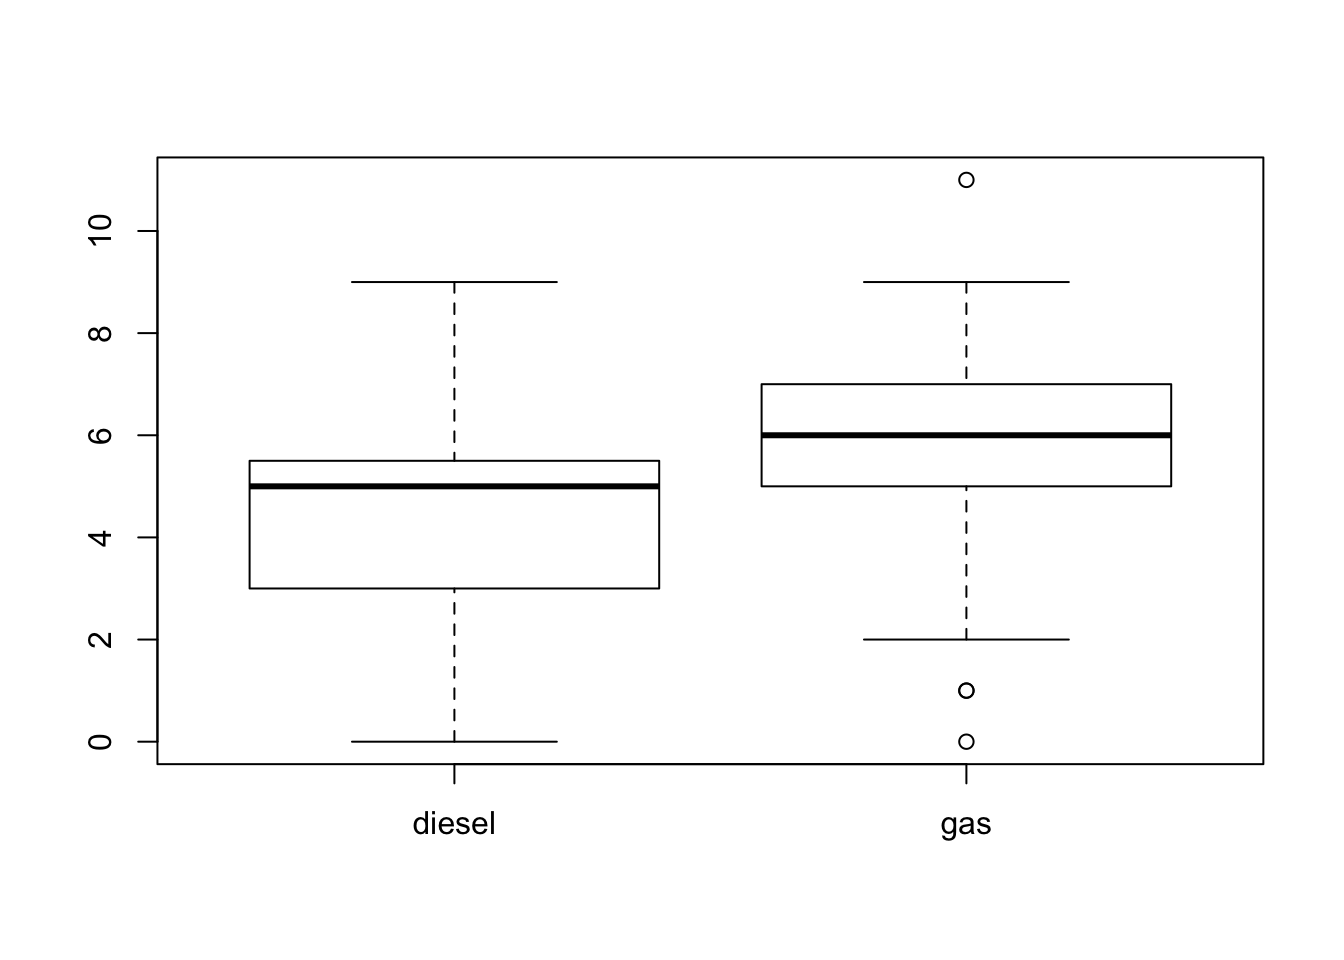
\includegraphics[width=0.6\linewidth]{statthink_files/figure-latex/Confidence1-1} 

}

\caption{Box Plots of Differences in MPG}\label{fig:Confidence1}
\end{figure}

We conduct inference for each fuel type separately. However, since the
sample size for cars that run on diesel is only 20, one may have
concerns regarding the application of methods that assume a large sample
size to a sample size this small.

\hypertarget{confidence-intervals-for-a-normal-mean}{%
\subsection{Confidence Intervals for a Normal Mean}\label{confidence-intervals-for-a-normal-mean}}

Consider the construction of a confidence interval for the expectation
of a Normal measurement. In the previous section, when dealing with the
construction of a confidence interval for the expectation, we exploited
the Central Limit Theorem in order to identify that the distribution of
the standardized sample average \((\bar X - \Expec(X))/\sqrt{\Var(X)/n}\)
is, approximately, standard Normal. Afterwards, we substituted the
standard deviation of the measurement by the sample standard deviation
\(S\), which was an accurate estimator of the former due to the magnitude
sample size.

In the case where the measurements themselves are Normally distributed
one can identify the exact distribution of the standardized sample
average, with the sample variance substituting the variance of the
measurement: \((\bar X - \Expec(X))/(S/\sqrt{n})\). This specific
distribution is called the Student's \(t\)-distribution, or simply the
\(t\)-distribution.

The \(t\)-distribution is bell shaped and symmetric. Overall, it looks
like the standard Normal distribution but it has wider tails. The
\(t\)-distribution is characterized by a parameter called the number of
\emph{degrees of freedom}. In the current setting, where we deal with the
standardized sample average (with the sample variance substituting the
variance of the measurement) the number of degrees of freedom equals the
number of observations associated with the estimation of the variance,
minus 1. Hence, if the sample size is \(n\) and if the measurement is
Normally distributed then the standardized sample average (with \(S\)
substituting the standard deviation of the measurement) has a
\(t\)-distribution on \((n-1)\) degrees of freedom. We use \(t_{(n-1)}\) to
denote this \(t\)-distribution.

The \texttt{R} system contains functions for the computation of the density,
the cumulative probability function and the percentiles of the
\(t\)-distribution, as well as for the simulation of a random sample from
this distribution. Specifically, the function ``\texttt{qt}'' computes the
percentiles of the \(t\)-distribution. The first argument to the function
is a probability and the second argument is the number of degrees of
freedom. The output of the function is the percentile associated with
the probability of the first argument. Namely, it is a value such that
the probability that the \(t\)-distribution is below the value is equal to
the probability in the first argument.

For example, let ``\texttt{n}'' be the sample size. The output of the expression
``\texttt{qt(0.975,n-1)}'' is the 0.975-percentile of the \(t\)-distribution on
\((n-1)\) degrees of freedom. By definition, 97.5\% of the \(t\)-distribution
are below this value and 2.5\% are above it. The symmetry of the \(t\)
distribution implies that 2.5\% of the distribution is below the negative
of this value. The middle part of the distribution is bracketed by these
two values:
\([-\mbox{\texttt{qt(0.975,n-1)}}, \mbox{\texttt{qt(0.975,n-1)}}]\), and
it contains 95\% of the distribution.

Summarizing the above claims in a single formula produces the statement:

\[\frac{\bar X - \Expec(X)}{S/\sqrt{n}} \sim t_{(n-1)} \quad \Longrightarrow \quad \Prob \bigg(\bigg|\frac{\bar X - \Expec(X)}{S/\sqrt{n}}\bigg| \leq \mbox{\texttt{qt(0.975,n-1)}} \bigg) = 0.95\;.\]
Notice that the equation associated with the probability is not an
approximation but an exact relation\footnote{When the measurement is Normally distributed.}. Rewriting the event that is
described in the probability in the form of a confidence interval,
produces

\[\bar X \pm \mbox{\texttt{qt(0.975,n-1)}}\cdot S/ \sqrt{n}\]
as a confidence interval for the expectation of the Normal measurement
with a confidence level of 95\%.

The structure of the confidence interval for the expectation of a Normal
measurement is essentially identical to the structure proposed in the
previous section. The only difference is that the number 1.96, the
percentile of the standard Normal distribution, is substituted by the
percentile of the \(t\)-distribution.

Consider the construction of a confidence interval for the expected
difference in fuel consumption between highway and urban driving
conditions. In order to save writing we created two new variables; a
factor called ``\texttt{fuel}'' that contains the data on the fuel type of each
car, and a numerical vector called ``\texttt{dif.mpg}'' that contains the
difference between highway and city fuel consumption for each car type:

\begin{Shaded}
\begin{Highlighting}[]
\NormalTok{fuel <-}\StringTok{ }\NormalTok{cars}\OperatorTok{$}\NormalTok{fuel.type}
\NormalTok{dif.mpg <-}\StringTok{ }\NormalTok{cars}\OperatorTok{$}\NormalTok{highway.mpg }\OperatorTok{-}\StringTok{ }\NormalTok{cars}\OperatorTok{$}\NormalTok{city.mpg}
\end{Highlighting}
\end{Shaded}

We are interested in confidence intervals based on the data stored in
the variable ``\texttt{dif.mpg}''. One confidence interval will be associated
with the level ``\texttt{diesel}'' of the factor ``\texttt{fuel}'' and the other will be
associated with the level ``\texttt{gas}'' of the same factor.

In order to compute these confidence intervals we need to compute, for
each level of the factor ``\texttt{fuel}'', the sample average and the sample
standard deviation of the data points of the variable ``\texttt{dif.mpg}'' that
are associated with that level.

It is convenient to use the function ``\texttt{tapply}'' for this task. This
function uses three arguments. The first argument is the sequence of
values over which we want to carry out some computation. The second
argument is a factor. The third argument is a name of a function that is
used for the computation. The function ``\texttt{tapply}'' applies the function
in the third argument to each sub-collection of values of the first
argument. The sub-collections are determined by the levels of the second
argument.

Sounds complex but it is straightforward enough to apply:

\begin{Shaded}
\begin{Highlighting}[]
\KeywordTok{tapply}\NormalTok{(dif.mpg,fuel,mean)}
\end{Highlighting}
\end{Shaded}

\begin{verbatim}
##    diesel       gas 
## 4.4500000 5.6486486
\end{verbatim}

\begin{Shaded}
\begin{Highlighting}[]
\KeywordTok{tapply}\NormalTok{(dif.mpg,fuel,sd)}
\end{Highlighting}
\end{Shaded}

\begin{verbatim}
##    diesel       gas 
## 2.7810449 1.4336070
\end{verbatim}

Sample averages are computed in the first application of the function
``\texttt{tapply}''. Observe that an average was computed for cars that run on
diesel and an average was computed for cars that run on gas. In both
cases the average corresponds to the difference in fuel consumption.
Similarly, the standard deviations were computed in the second
application of the function. We obtain that the point estimates of the
expectation for diesel and gas cars are 4.45 and 5.648649, respectively
and the point estimates for the standard deviation of the variable are
2.781045 and 1.433607.

Let us compute the confidence interval for each type of fuel:

\begin{Shaded}
\begin{Highlighting}[]
\NormalTok{x.bar <-}\StringTok{ }\KeywordTok{tapply}\NormalTok{(dif.mpg,fuel,mean)}
\NormalTok{s <-}\StringTok{ }\KeywordTok{tapply}\NormalTok{(dif.mpg,fuel,sd)}
\NormalTok{n <-}\StringTok{ }\KeywordTok{c}\NormalTok{(}\DecValTok{20}\NormalTok{,}\DecValTok{185}\NormalTok{)}
\NormalTok{x.bar }\OperatorTok{-}\StringTok{ }\KeywordTok{qt}\NormalTok{(}\FloatTok{0.975}\NormalTok{,n}\DecValTok{-1}\NormalTok{)}\OperatorTok{*}\NormalTok{s}\OperatorTok{/}\KeywordTok{sqrt}\NormalTok{(n)}
\end{Highlighting}
\end{Shaded}

\begin{verbatim}
##    diesel       gas 
## 3.1484309 5.4406990
\end{verbatim}

\begin{Shaded}
\begin{Highlighting}[]
\NormalTok{x.bar }\OperatorTok{+}\StringTok{ }\KeywordTok{qt}\NormalTok{(}\FloatTok{0.975}\NormalTok{,n}\DecValTok{-1}\NormalTok{)}\OperatorTok{*}\NormalTok{s}\OperatorTok{/}\KeywordTok{sqrt}\NormalTok{(n)}
\end{Highlighting}
\end{Shaded}

\begin{verbatim}
##    diesel       gas 
## 5.7515691 5.8565983
\end{verbatim}

The objects ``\texttt{x.bar}'' and ``\texttt{s}'' contain the sample averages and sample
standard deviations, respectively. Both are sequences of length two,
with the first component referring to ``\texttt{diesel}'' and the second
component referring to ``\texttt{gas}''. The object ``\texttt{n}'' contains the two sample
sizes, 20 for ``\texttt{diesel}'' and 185 for ``\texttt{gas}''. In the expression next to
last the lower boundary for each of the confidence intervals is computed
and in the last expression the upper boundary is computed. The
confidence interval for the expected difference in diesel cars is
\([3.148431, 5.751569]\). and the confidence interval for cars using gas
is \([5.440699, 5.856598]\).

The 0.975-percentiles of the \(t\)-distributions are computed with the
expressions ``\texttt{qt(0.025,n-1)}'':

\begin{Shaded}
\begin{Highlighting}[]
\KeywordTok{qt}\NormalTok{(}\FloatTok{0.975}\NormalTok{,n}\DecValTok{-1}\NormalTok{)}
\end{Highlighting}
\end{Shaded}

\begin{verbatim}
## [1] 2.0930241 1.9729405
\end{verbatim}

The second argument of the function ``\texttt{qt}'' is a sequence with two
components, the number 19 and the number 184. Accordingly, The first
position in the output of the function is the percentile associated with
19 degrees of freedom and the second position is the percentile
associated to 184 degrees of freedom.

Compare the resulting percentiles to the 0.975-percentile of the
standard Normal distribution, which is essentially equal to 1.96. When
the sample size is small, 20 for example, the percentile of the
\(t\)-distribution is noticeably larger than the percentile of the
standard Normal. However, for a larger sample size the percentiles, more
or less, coincide. It follows that for a large sample the method
proposed in Subsection~\ref{subsec:CImean} and the method
discussed in this subsection produce essentially the same confidence
intervals.

\hypertarget{confidence-intervals-for-a-normal-variance}{%
\subsection{Confidence Intervals for a Normal Variance}\label{confidence-intervals-for-a-normal-variance}}

The next task is to compute confidence intervals for the variance of a
Normal measurement. The main idea in the construction of a confidence
interval is to identify the distribution of a random variable associated
with the parameter of interest. A region that contains 95\% of the
distribution of the random variable (or, more generally, the central
part of the distribution of probability equal to the confidence level)
is identified. The confidence interval results from the reformulation of
the event associated with that region. The new formulation puts the
parameter between a lower limit and an upper limit. These lower and the
upper limits are computed from the data and they form the boundaries of
the confidence interval.

We start with the sample variance,
\(S^2 = \sum_{i=1}^n (X_i - \bar X)^2/(n-1)\), which serves as a point
estimator of the parameter of interest. When the measurements are
Normally distributed then the random variable \((n-1)S^2/\sigma^2\)
possesses a special distribution called the chi-square distribution.
(Chi is the Greek letter \(\chi\), which is read ``Kai''.) This distribution
is associated with the sum of squares of Normal variables. It is
parameterized, just like the \(t\)-distribution, by a parameter called the
number of degrees of freedom. This number is equal to \((n-1)\) in the
situation we discuss. The chi-square distribution on \((n-1)\) degrees of
freedom is denoted with the symbol \(\chi^2_{(n-1)}\).

The \texttt{R} system contains functions for the computation of the density,
the cumulative probability function and the percentiles of the
chi-square distribution, as well as for the simulation of a random
sample from this distribution. Specifically, the percentiles of the
chi-square distribution are computed with the aid of the function
``\texttt{qchisq}''. The first argument to the function is a probability and the
second argument is the number of degrees of freedom. The output of the
function is the percentile associated with the probability of the first
argument. Namely, it is a value such that the probability that the
chi-square distribution is below the value is equal to the probability
in the first argument.

For example, let ``\texttt{n}'' be the sample size. The output of the expression
``\texttt{qt(0.975,n-1)}'' is the 0.975-percentile of the chi-square
distribution. By definition, 97.5\% of the chi-square distribution are
below this value and 2.5\% are above it. Similarly, the expression
``\texttt{qchisq(0.025,n-1)}'' is the 0.025-percentile of the chi-square
distribution, with 2.5\% of the distribution below this value. Notice
that between these two percentiles, namely within the interval
\([\mbox{\texttt{qchisq(0.025,n-1)}}, \mbox{\texttt{qchisq(0.975,n-1)}}]\),
are 95\% of the chi-square distribution.

We may summarize that for Normal measurements:

\[\begin{aligned}
\lefteqn{(n-1)S^2/\sigma^2 \sim \chi^2_{(n-1)} \quad \Longrightarrow }\\ & \Prob \big( \mbox{\texttt{qchisq(0.025,n-1)}} \leq (n-1)S^2/\sigma^2  \leq \mbox{\texttt{qchisq(0.975,n-1)}} \big) = 0.95\;.\end{aligned}\]
The chi-square distribution is not symmetric. Therefore, in order to
identify the region that contains 95\% of the distribution region we have
to compute both the 0.025- and the 0.975-percentiles of the
distribution.

The event associated with the 95\% region is rewritten in a form that
puts the parameter \(\sigma^2\) in the center:

\[\big\{(n-1)S^2/\mbox{\texttt{qchisq(0.975,n-1)}} \leq  \sigma^2  \leq (n-1)S^2/\mbox{\texttt{qchisq(0.025,n-1)}}\big\}\;.\]
The left most and the right most expressions in this event mark the end
points of the confidence interval. The structure of the confidence
interval is:

\[\big[\{(n-1)/\mbox{\texttt{qchisq(0.975,n-1)}}\}\times S^2,\;\{(n-1)/\mbox{\texttt{qchisq(0.025,n-1)}}\}\times S^2\big]\;.\]
Consequently, the confidence interval is obtained by the multiplication
of the estimator of the variance by a ratio between the number of
degrees of freedom (\(n-1\)) and an appropriate percentile of the
chi-square distribution. The percentile on the left hand side is
associated with the larger probability (making the ratio smaller) and
the percentile on the right hand side is associated with the smaller
probability (making the ratio larger).

Consider, specifically, the confidence intervals for the variance of the
measurement ``\texttt{diff.mpg}'' for cars that run on diesel and for cars that
run on gas. Here, the size of the samples is 20 and 185, respectively:

\begin{Shaded}
\begin{Highlighting}[]
\NormalTok{(n}\DecValTok{-1}\NormalTok{)}\OperatorTok{/}\KeywordTok{qchisq}\NormalTok{(}\FloatTok{0.975}\NormalTok{,n}\DecValTok{-1}\NormalTok{)}
\end{Highlighting}
\end{Shaded}

\begin{verbatim}
## [1] 0.57834564 0.82342954
\end{verbatim}

\begin{Shaded}
\begin{Highlighting}[]
\NormalTok{(n}\DecValTok{-1}\NormalTok{)}\OperatorTok{/}\KeywordTok{qchisq}\NormalTok{(}\FloatTok{0.025}\NormalTok{,n}\DecValTok{-1}\NormalTok{)}
\end{Highlighting}
\end{Shaded}

\begin{verbatim}
## [1] 2.1332695 1.2404776
\end{verbatim}

The ratios that are used in the left hand side of the intervals are
0.5783456 and 0.8234295, respectively. Both ratios are less than one. On
the other hand, the ratios associated with the other end of the
intervals, 2.133270 and 1.240478, are both larger than one.

Let us compute the point estimates of the variance and the associated
confidence intervals. Recall that the object ``\texttt{s}'' contains the sample
standard deviations of the difference in fuel consumption for diesel and
for gas cars. The object ``\texttt{n}'' contains the two sample sizes:

\begin{Shaded}
\begin{Highlighting}[]
\NormalTok{s}\OperatorTok{^}\DecValTok{2}
\end{Highlighting}
\end{Shaded}

\begin{verbatim}
##    diesel       gas 
## 7.7342105 2.0552291
\end{verbatim}

\begin{Shaded}
\begin{Highlighting}[]
\NormalTok{(n}\DecValTok{-1}\NormalTok{)}\OperatorTok{*}\NormalTok{s}\OperatorTok{^}\DecValTok{2}\OperatorTok{/}\KeywordTok{qchisq}\NormalTok{(}\FloatTok{0.975}\NormalTok{,n}\DecValTok{-1}\NormalTok{)}
\end{Highlighting}
\end{Shaded}

\begin{verbatim}
##    diesel       gas 
## 4.4730469 1.6923364
\end{verbatim}

\begin{Shaded}
\begin{Highlighting}[]
\NormalTok{(n}\DecValTok{-1}\NormalTok{)}\OperatorTok{*}\NormalTok{s}\OperatorTok{^}\DecValTok{2}\OperatorTok{/}\KeywordTok{qchisq}\NormalTok{(}\FloatTok{0.025}\NormalTok{,n}\DecValTok{-1}\NormalTok{)}
\end{Highlighting}
\end{Shaded}

\begin{verbatim}
##     diesel        gas 
## 16.4991555  2.5494656
\end{verbatim}

The variance of the difference in fuel consumption for diesel cars is
estimated to be 7.734211 with a 95\%-confidence interval of
\([4.473047, 16.499155]\) and for cars that use gas the estimated variance
is 2.055229, with a confidence interval of \([1.692336, 2.549466]\).

As a final example in this section let us simulate the confidence level
for a confidence interval for the expectation and for a confidence
interval for the variance of a Normal measurement. In this simulation we
assume that the expectation is equal to \(\mu = 3\) and the variance is
equal to \(\sigma^2 = 3^2 = 9\). The sample size is taken to be \(n=20\). We
start by producing the sampling distribution of the sample average
\(\bar X\) and of the sample standard deviation \(S\):

\begin{Shaded}
\begin{Highlighting}[]
\NormalTok{mu <-}\StringTok{ }\DecValTok{4}
\NormalTok{sig <-}\StringTok{ }\DecValTok{3}
\NormalTok{n <-}\StringTok{ }\DecValTok{20}
\NormalTok{X.bar <-}\StringTok{ }\KeywordTok{rep}\NormalTok{(}\DecValTok{0}\NormalTok{,}\DecValTok{10}\OperatorTok{^}\DecValTok{5}\NormalTok{)}
\NormalTok{S <-}\StringTok{ }\KeywordTok{rep}\NormalTok{(}\DecValTok{0}\NormalTok{,}\DecValTok{10}\OperatorTok{^}\DecValTok{5}\NormalTok{)}
\ControlFlowTok{for}\NormalTok{(i }\ControlFlowTok{in} \DecValTok{1}\OperatorTok{:}\DecValTok{10}\OperatorTok{^}\DecValTok{5}\NormalTok{) \{}
\NormalTok{  X <-}\StringTok{ }\KeywordTok{rnorm}\NormalTok{(n,mu,sig)}
\NormalTok{  X.bar[i] <-}\StringTok{ }\KeywordTok{mean}\NormalTok{(X)}
\NormalTok{  S[i] <-}\StringTok{ }\KeywordTok{sd}\NormalTok{(X)}
\NormalTok{\}}
\end{Highlighting}
\end{Shaded}

Consider first the confidence interval for the expectation:

\begin{Shaded}
\begin{Highlighting}[]
\NormalTok{mu.LCL <-}\StringTok{ }\NormalTok{X.bar }\OperatorTok{-}\StringTok{ }\KeywordTok{qt}\NormalTok{(}\FloatTok{0.975}\NormalTok{,n}\DecValTok{-1}\NormalTok{)}\OperatorTok{*}\NormalTok{S}\OperatorTok{/}\KeywordTok{sqrt}\NormalTok{(n)}
\NormalTok{mu.UCL <-}\StringTok{ }\NormalTok{X.bar }\OperatorTok{+}\StringTok{ }\KeywordTok{qt}\NormalTok{(}\FloatTok{0.975}\NormalTok{,n}\DecValTok{-1}\NormalTok{)}\OperatorTok{*}\NormalTok{S}\OperatorTok{/}\KeywordTok{sqrt}\NormalTok{(n)}
\KeywordTok{mean}\NormalTok{((mu }\OperatorTok{>=}\StringTok{ }\NormalTok{mu.LCL) }\OperatorTok{&}\StringTok{ }\NormalTok{(mu }\OperatorTok{<=}\StringTok{ }\NormalTok{mu.UCL))}
\end{Highlighting}
\end{Shaded}

\begin{verbatim}
## [1] 0.95011
\end{verbatim}

The nominal significance level of the confidence interval is 95\%, which
is practically identical to the confidence level that was computed in
the simulation.

The confidence interval for the variance is obtained in a similar way.
The only difference is that we apply now different formulae for the
computation of the upper and lower confidence limits:

\begin{Shaded}
\begin{Highlighting}[]
\NormalTok{var.LCL <-}\StringTok{ }\NormalTok{(n}\DecValTok{-1}\NormalTok{)}\OperatorTok{*}\NormalTok{S}\OperatorTok{^}\DecValTok{2}\OperatorTok{/}\KeywordTok{qchisq}\NormalTok{(}\FloatTok{0.975}\NormalTok{,n}\DecValTok{-1}\NormalTok{)}
\NormalTok{var.UCL <-}\StringTok{ }\NormalTok{(n}\DecValTok{-1}\NormalTok{)}\OperatorTok{*}\NormalTok{S}\OperatorTok{^}\DecValTok{2}\OperatorTok{/}\KeywordTok{qchisq}\NormalTok{(}\FloatTok{0.025}\NormalTok{,n}\DecValTok{-1}\NormalTok{)}
\KeywordTok{mean}\NormalTok{((sig}\OperatorTok{^}\DecValTok{2} \OperatorTok{>=}\StringTok{ }\NormalTok{var.LCL) }\OperatorTok{&}\StringTok{ }\NormalTok{(sig}\OperatorTok{^}\DecValTok{2} \OperatorTok{<=}\StringTok{ }\NormalTok{var.UCL))}
\end{Highlighting}
\end{Shaded}

\begin{verbatim}
## [1] 0.95083
\end{verbatim}

Again, we obtain that the nominal confidence level of 95\% coincides with
the confidence level computed in the simulation.

\hypertarget{choosing-the-sample-size}{%
\section{Choosing the Sample Size}\label{choosing-the-sample-size}}

One of the more important contributions of Statistics to research is
providing guidelines for the design of experiments and surveys. A well
planed experiment may produce accurate enough answers to the research
questions while optimizing the use of resources. On the other hand,
poorly planed trials may fail to produce such answers or may waste
valuable resources.

Unfortunately, in this book we do not cover the subject of experiment
design. Still, we would like to give a brief discussion of a narrow
aspect in design: The selection of the sample size.

An important consideration at the stage of the planning of an experiment
or a survey is the number of observations that should be collected.
Indeed, having a larger sample size is usually preferable from the
statistical point of view. However, an increase in the sample size
typically involves an increase in expenses. Thereby, one would prefer to
collect the minimal number of observations that is still sufficient in
order to reach a valid conclusion.

As an example, consider an opinion poll aimed at the estimation of the
proportion in the population of those that support a specific candidate
that considers running for an office. How large the sample must be in
order to assure, with high probability, that the percentage in the
sample of supporters is within 0.5\% of the percentage in the population?
Within 0.25\%?

A natural way to address this problem is via a confidence interval for
the proportion. If the range of the confidence interval is no more than
0.05 (or 0.025 in the other case) then with a probability equal to the
confidence level it is assured that the population relative frequency is
within the given distance from the sample proportion.

Consider a confidence level of 95\%. Recall that the structure of the
confidence interval for the proportion is
\(\hat P \pm 1.96 \cdot \{\hat P (1-\hat P)/n\}^{1/2}\). The range of the
confidence interval is \(1.96 \cdot \{\hat P (1-\hat P)/n\}^{1/2}\). How
large should \(n\) be in order to guarantee that the range is no more than
0.05?

The answer to this question depends on the magnitude of
\(\hat P (1-\hat P)\), which is a random quantity. Luckily, one may
observe that the maximal value\footnote{The derivative is \(f'(p) = 1-2p\). Solving \(f'(p)=0\) produces
  \(p=1/2\) as the maximizer. Plugging this value in the function gives
  \(1/4\) as the maximal value of the function.} of the quadratic function
\(f(p) = p (1-p)\) is 1/4. It follows that

\[1.96 \cdot \{\hat P (1-\hat P)/n\}^{1/2} \leq 1.96 \cdot \{0.25/n\}^{1/2} = 0.98/\sqrt{n}\;.\]
Finally,

\[0.98/\sqrt{n} \leq 0.05 \quad \Longrightarrow \quad \sqrt{n} \geq 0.98/0.05 = 19.6
\quad \Longrightarrow \quad  n \geq (19.6)^2 = 384.16\;.\] The
conclusion is that \(n\) should be larger than 384 in order to assure the
given range. For example, \(n=385\) should be sufficient.

If the request is for an interval of range 0.025 then the last line of
reasoning should be modified accordingly:

\[0.98/\sqrt{n} \leq 0.025 \quad \Longrightarrow \quad \sqrt{n} \geq \frac{0.98}{0.025} = 39.2
\quad \Longrightarrow \quad  n \geq (39.2)^2 = 1536.64\;.\]
Consequently, \(n=1537\) will do. Increasing the accuracy by 50\% requires
a sample size that is 4 times larger.

More examples that involve selection of the sample size will be
considered as part of the homework.

\hypertarget{exercises-6}{%
\section{Exercises}\label{exercises-6}}

\BeginKnitrBlock{exercise}
\protect\hypertarget{exr:unnamed-chunk-169}{}{\label{exr:unnamed-chunk-169} }This exercise deals with an experiment that was
conducted among students. The aim of the experiment was to assess the
effect of rumors and prior reputation of the instructor on the
evaluation of the instructor by her students. The experiment was
conducted by Towler and Dipboye\footnote{Towler, A. and Dipboye, R. L. (1998). The effect of instructor
  reputation and need for cognition on student behavior (poster
  presented at American Psychological Society conference, May 1998).}. This case study is taken from the
\href{http://onlinestatbook.com/rvls.html}{Rice Virtual Lab in Statistics}.
More details on this case study can be found in the case study
``\href{http://onlinestatbook.com/case_studies_rvls/instructor_reputation/index.html}{Instructor Reputation and Teacher
Ratings}''
that is presented in that site.

The experiment involved 49 students that were randomly assigned to one
of two conditions. Before viewing the lecture, students were give one of
two ``summaries'' of the instructor's prior teaching evaluations. The
first type of summary, i.e.~the first condition, described the lecturer
as a charismatic instructor. The second type of summary (second
condition) described the lecturer as a punitive instructor. We code the
first condition as ``\texttt{C}'' and the second condition as ``\texttt{P}''. All subjects
watched the same twenty-minute lecture given by the exact same lecturer.
Following the lecture, subjects rated the lecturer.

The outcomes are stored in the file ``\texttt{teacher.csv}''. The file can be
found on the internet at
\url{http://pluto.huji.ac.il/~msby/StatThink/Datasets/teacher.csv}. Download
this file to your computer and store it in the working directory of \texttt{R}.
Read the content of the file into an \texttt{R} data frame. Produce a summary
of the content of the data frame and answer the following questions:

\begin{enumerate}
\def\labelenumi{\arabic{enumi}.}
\item
  Identify, for each variable in the file ``\texttt{teacher.csv}'', the name
  and the type of the variable (factor or numeric).
\item
  Estimate the expectation and the standard deviation among all
  students of the rating of the teacher.
\item
  Estimate the expectation and the standard deviation of the rating
  only for students who were given a summary that describes the
  teacher as charismatic.
\item
  Construct a confidence interval of 99\% confidence level for the
  expectation of the rating among students who were given a summary
  that describes the teacher as charismatic. (Assume the ratings have
  a Normal distribution.)
\item
  Construct a confidence interval of 90\% confidence level for the
  variance of the rating among students who were given a summary that
  describes the teacher as charismatic. (Assume the ratings have a
  Normal distribution.)
\end{enumerate}
\EndKnitrBlock{exercise}

\BeginKnitrBlock{exercise}
\protect\hypertarget{exr:unnamed-chunk-170}{}{\label{exr:unnamed-chunk-170} }Twenty observations are used in order to construct a
confidence interval for the expectation. In one case, the construction
is based on the Normal approximation of the sample average and in the
other case it is constructed under the assumption that the observations
are Normally distributed. Assume that in reality the measurement is
distributed \(\mathrm{Exponential}(1/4)\).

\begin{enumerate}
\def\labelenumi{\arabic{enumi}.}
\item
  Compute, via simulation, the actual confidence level for the first
  case of a confidence interval with a nominal confidence level of
  95\%.
\item
  Compute, via simulation, the actual confidence level for the second
  case of a confidence interval with a nominal confidence level of
  95\%.
\item
  Which of the two approaches would you prefer?
\end{enumerate}
\EndKnitrBlock{exercise}

\BeginKnitrBlock{exercise}
\protect\hypertarget{exr:unnamed-chunk-171}{}{\label{exr:unnamed-chunk-171} }Insurance companies are interested in knowing the
population percent of drivers who always buckle up before riding in a
car.

\begin{enumerate}
\def\labelenumi{\arabic{enumi}.}
\item
  When designing a study to determine this proportion, what is the
  minimal sample size that is required for a 99\% confident that the
  population proportion is accurately estimated, up to an error of
  0.03?
\item
  Suppose that the insurance companies did conduct the study by
  surveying 400 drivers. They found that 320 of the drives claim to
  always buckle up. Produce an 80\% confidence interval for the
  population proportion of drivers who claim to always buckle up.
\end{enumerate}
\EndKnitrBlock{exercise}

\hypertarget{summary-9}{%
\section{Summary}\label{summary-9}}

\hypertarget{glossary}{%
\subsection*{Glossary}\label{glossary}}


\begin{description}
\item[Confidence Interval:]
An interval that is most likely to contain the population parameter.
\item[Confidence Level:]
The sampling probability that random confidence intervals contain
the parameter value. The confidence level of an observed interval
indicates that it was constructed using a formula that produces,
when applied to random samples, such random intervals.
\item[t-Distribution:]
A bell-shaped distribution that resembles the standard Normal
distribution but has wider tails. The distribution is characterized
by a positive parameter called \emph{degrees of freedom}.
\item[Chi-Square Distribution:]
A distribution associated with the sum of squares of Normal random
variable. The distribution obtains only positive values and it is
not symmetric. The distribution is characterized by a positive
parameter called \emph{degrees of freedom}.
\end{description}

\hypertarget{discuss-in-the-forum}{%
\subsection*{Discuss in the forum}\label{discuss-in-the-forum}}


When large samples are at hand one may make fewer a-priori assumptions
regarding the exact form of the distribution of the measurement. General
limit theorems, such as the Central Limit Theorem, may be used in order
to establish the validity of the inference under general conditions. On
the other hand, for small sample sizes one must make strong assumptions
with respect to the distribution of the observations in order to justify
the validity of the procedure.

It may be claimed that making statistical inferences when the sample
size is small is worthless. How can one trust conclusions that depend on
assumptions regarding the distribution of the observations, assumptions
that cannot be verified? What is your opinion?

For illustration consider the construction of a confidence interval.
Confidence interval for the expectation is implemented with a specific
formula. The significance level of the interval is provable when the
sample size is large or when the sample size is small but the
observations have a Normal distribution. If the sample size is small and
the observations have a distribution different from the Normal then the
nominal significance level may not coincide with the actual significance
level.

\hypertarget{formulas-for-confidence-intervals-95-confidence-level}{%
\subsection*{Formulas for Confidence Intervals, 95\% Confidence Level:}\label{formulas-for-confidence-intervals-95-confidence-level}}


\begin{itemize}
\item
  Expectation:
  \(\bar x \pm \mbox{\texttt{qnorm(0.975)}} \cdot s/\sqrt{n}\).
\item
  Probability:
  \(\bar p \pm \mbox{\texttt{qnorm(0.975)}} \cdot \hat p(1-\hat p)/\sqrt{n}\).
\item
  Normal Expectation:
  \(\bar x \pm \mbox{\texttt{qt(0.975,n-1)}} \cdot s/\sqrt{n}\).
\item
  Normal Expectation:
  \(\big[\frac{n-1}{\mbox{\texttt{qchisq(0.975,n-1)}}} s^2 ,\;\frac{n-1}{\mbox{\texttt{qchisq(0.025,n-1)}}} s^2\big]\).
\end{itemize}

\hypertarget{ChapTesting}{%
\chapter{Testing Hypothesis}\label{ChapTesting}}

\hypertarget{student-learning-objectives-6}{%
\section{Student Learning Objectives}\label{student-learning-objectives-6}}

Hypothesis testing emerges as a crucial component in decision making
where one of two competing options needs to be selected. Statistical
hypothesis testing provides formal guidelines for making such a
selection. This chapter deals with the formulation of statistical
hypothesis testing and describes the associated decision rules.
Specifically, we consider hypothesis testing in the context of the
expectation of a measurement and in the context of the probability of an
event. In subsequent chapters we deal with hypothesis testing in the
context of other parameters as well. By the end of this chapter, the
student should be able to:

\begin{itemize}
\item
  Formulate statistical hypothesis for testing.
\item
  Test, based on a sample, hypotheses regarding the expectation of the
  measurement and the probability of an event.
\item
  Identify the limitations of statistical hypothesis testing and the
  danger of misinterpretation of the test's conclusions.
\end{itemize}

\hypertarget{the-theory-of-hypothesis-testing}{%
\section{The Theory of Hypothesis Testing}\label{the-theory-of-hypothesis-testing}}

Statistical inference is used in order to detect and characterize
meaningful phenomena that may be hidden in an environment contaminated
by random noise. Hypothesis testing is an important step, typically the
first, in the process of making inferences. In this step one tries to
answer the question: ``Is there a phenomena at all?''. The basic approach
is to determine whether the observed data can or cannot be reasonably
explained by a model of randomness that does not involve the phenomena.

In this section we introduce the structure and characteristics of
statistical hypothesis testing. We start with an informal application of
a statistical test and proceed with formal definitions. In the next
section we discuss in more detail the testing of hypotheses on the
expectation of a measurement and the testing of hypotheses on the
probability of an event. More examples are considered in subsequent
chapters.

\hypertarget{an-example-of-hypothesis-testing}{%
\subsection{An Example of Hypothesis Testing}\label{an-example-of-hypothesis-testing}}

The variable ``\texttt{price}'' in the file ``\texttt{cars.csv}'' contains data on the
prices of different types of cars that were sold in the United States
during 1985. The average price of a car back then --- the average of the
variable ``\texttt{price}'' --- was \$13,207. One may be interested in the
question: Do Americans pay today for cars a different price than what
they used to pay in the 80's? Has the price of cars changed
significantly since 1985?

The average price of a car in the United States in 2009 was
\$27,958\footnote{Source:
  ``\url{http://wiki.answers.com/Q/Average_price_of_a_car_in_2009}''.}. Clearly, this figure is higher than \$13,207. However, in
order to produce a fair answer to the question we have to take into
account that, due to inflation, the prices of all products went up
during these years. A more meaningful comparison will involve the
current prices of cars in terms of 1985 Dollars. Indeed, if we take into
account inflation then we get that, on the average, the cost of today's
cars corresponds to an average price of \$13,662 in 1985 values\footnote{Source: ``\url{http://www.westegg.com/inflation/}''. The interpretation
  of adjusting prices to inflation is that our comparison will
  correspond to changes in the price of cars, relative to other items
  that enter into the computation of the Consumer Price Index.}.
This price is still higher than the prices in the 1985 but not as much.
The question we are asking is: ``Is the difference between \$13,207 and
\$13,662 significant or is it not so?''.

In order to give a statistical answer to this question we carry out a
statistical test. The specific test is conducted with the aid of the
function ``\texttt{t.test}''. Later we will discuss in more details some of the
arguments that may be used in this function. Currently, we simply apply
it to the data stored in the variable ``\texttt{price}'' to test that the
expected price is different than the \$13,662, the average price of a
car in 2009, adjusted for inflation:

\begin{Shaded}
\begin{Highlighting}[]
\NormalTok{cars <-}\StringTok{ }\KeywordTok{read.csv}\NormalTok{(}\StringTok{"_data/cars.csv"}\NormalTok{)}
\KeywordTok{t.test}\NormalTok{(cars}\OperatorTok{$}\NormalTok{price,}\DataTypeTok{mu=}\DecValTok{13662}\NormalTok{)}
\end{Highlighting}
\end{Shaded}

\begin{verbatim}
## 
##  One Sample t-test
## 
## data:  cars$price
## t = -0.811482, df = 200, p-value = 0.41805
## alternative hypothesis: true mean is not equal to 13662
## 95 percent confidence interval:
##  12101.797 14312.462
## sample estimates:
## mean of x 
## 13207.129
\end{verbatim}

The data in the file ``\texttt{cars.csv}'' is read into a data frame that is
given the name ``\texttt{cars}''. Afterwards, the data on prices of car types in
1985 is entered as the first argument to the function ``\texttt{t.test}''. The
other argument is the expected value that we want to test, the current
average price of cars, given in terms of 1985 Dollar value. The output
of the function is reported under the title: ``\texttt{One\ Sample\ t-test}''.

Let us read the report from the bottom up. The bottom part of the report
describes the confidence interval and the point estimate of the expected
price of a car in 1985, based on the given data. Indeed, the last line
reports the sample average of the price, which is equal to 13,207.13.
This number, the average of the 201 non-missing values of the variable
``\texttt{price}'', serves as the estimate of the expected price of a car in
1985. The 95\% confidence interval of the expectation, the interval
\[12101.80, 14312.46\], is presented on the 4th line from the bottom.
This is the confidence interval for the expectation that was computed in
Subsection~\ref{subsec:CImean}\footnote{As a matter of fact, the confidence interval computed in
  Subsection~\[subsec:Confidence\_2.1\] is \[12108.47, 14305.79\],
  which is not identical to the confidence that appears in the report.
  The reason for the discrepancy is that we used the 0.975-percentile
  of the Normal distribution, 1.96, whereas the confidence interval
  computed here uses the 0.975-percentile of the \(t\)-distribution on
  201-1=200 degrees of freedom. The latter is equal to 1.971896.
  Nonetheless, for all practical purposes, the two confidence
  intervals are the same.}.

The information relevant to conducting the statistical test itself is
given in the upper part of the report. Specifically, it is reported that
the data in ``\texttt{cars\$price}'' is used in order to carry out the test. Based
on this data a test statistic is computed and obtains the value of
``\texttt{t\ =\ -0.8115}''. This statistic is associated with the \(t\)-distribution
with ``\texttt{df\ =\ 200}'' degrees of freedom. The last quantity that is being
reported is denoted the \emph{\(p\)-value} and it obtains the value
``\texttt{p-value\ =\ 0.4181}''. The test may be carried out with the aid of the
value of the \(t\) statistic or, more directly, using the \(p\)-value.
Currently we will use the \(p\)-value.

The test itself examines the hypothesis that the expected price of a car
in 1985 was equal to \$13,662, the average price of a car in 2009, given
in 1985 values. This hypothesis is called the null hypothesis. The
alternative hypothesis is that the expected price of a car in 1985 was
not equal to that figure. The specification of the alternative
hypothesis is reported on the third line of the output of the function
``\texttt{t.test}''.

One may decide between the two hypothesis on the basis of the size of
the \(p\)-value. The rule of thumb is to reject the null hypothesis, and
thus accept the alternative hypothesis, if the \(p\)-value is less than
0.05. In the current example the \(p\)-value is equal 0.4181 and is larger
than 0.05. Consequently, we may conclude that the expected price of a
car in 1985 was not significantly different than the current price of a
car.

In the rest of this section we give a more rigorous explanation of the
theory and practice of statistical hypothesis testing.

\hypertarget{the-structure-of-a-statistical-test-of-hypotheses}{%
\subsection{The Structure of a Statistical Test of Hypotheses}\label{the-structure-of-a-statistical-test-of-hypotheses}}

The initial step in statistical inference in general, and in statistical
hypothesis testing in particular, is the formulation of the statistical
model and the identification of the parameter/s that should be
investigated. In the current situation the statistical model may
correspond to the assumption that the data in the variable ``\texttt{price}'' are
an instance of a \emph{random} sample (of size \(n=201\)). The parameter that
we want to investigate is the expectation of the measurement that
produced the sample. The variance of the measurement is also relevant
for the investigation.

After the statistical model has been set, one may split the process of
testing a statistical hypothesis into three steps: (i) formulation of
the hypotheses, (ii) specification of the test, and (iii) reaching the
final conclusion. The first two steps are carried out on the basis of
the probabilistic characteristics of the statistical model and in the
context of the sampling distribution. In principal, the first two steps
may be conducted in the planning stage prior to the collection of the
observations. Only the third step involves the actual data. In the
example that was considered in the previous subsection the third step
was applied to the data in the variable ``\texttt{price}'' using the function
``\texttt{t.test}''.

{\textbf{(i) Formulating the hypotheses}}: A statistical model involves a
parameter that is the target of the investigation. In principle, this
parameter may obtain any value within a range of possible values. The
formulation of the hypothesis corresponds to splitting the range of
values into two sub-collections: a sub-collection that emerges in
response to the presence of the phenomena and a sub-collection that
emerges in response to the situation when the phenomena is absent. The
sub-collection of parameter values where the phenomena is absent is
called the \emph{null hypothesis} and is marked as ``\(H_0\)''. The other
sub-collection, the one reflecting the presence of the phenomena, is
denoted the \emph{alternative hypothesis} and is marked ``\(H_1\)''.

For example, consider the price of cars. Assume that the phenomena one
wishes to investigate is the change in the relative price of a car in
the 80's as compared to prices today. The parameter of interest is the
expected price of cars back then, which we denote by \(\Expec(X)\). The
formulation of the statement that the expected price of cars has changed
is ``\(\Expec(X) \not = 13,662\)''. This statement corresponds to the
\emph{presence} of a phenomena, to a change, and is customarily defined as
the alternative hypothesis. On the other hand, the situation
``\(\Expec(X) = 13,662\)'' corresponds to not having any change in the price
of cars. Hence, this situation corresponds to the \emph{absence} of the
phenomena and is denoted the null hypothesis. In summary, in order to
investigate the change in the relative price of cars we my consider the
null hypothesis ``\(H_0:\Expec(X) = 13,662\)'' and test it against the
alternative hypothesis ``\(H_1: \Expec(X)\not = 13,662\)''.

A variation in the formulation of the phenomena can change the
definition of the null and alternative hypotheses. For example, if the
intention is to investigate the \emph{rise} in the price of cars then the
phenomena will correspond to the expected price in 1985 being less than
\$13,662. Accordingly, the alternative hypothesis should be defined as
\(H_1: \Expec(X) < 13,662\), with the null hypothesis defined as
\(H_0: \Expec(X) \geq 13,662\). Observe that in this case an expected
price larger than \$13,662 relates to the phenomena of rising (relative)
prices \emph{not} taking place.

On the other hand, if one would wants to investigate a \emph{decrease} in the
price then one should define the alternative hypothesis to be
\(H_1: \Expec(X) > 13,662\), with the null hypothesis being
\(H_0: \Expec(X) \leq 13,662\).

The type of alternative that was considered in the example,
\(H_1: \Expec(X) \not = 13,622\) is called a \emph{two-sided} alternative. The
other two types of alternative hypotheses that were considered
thereafter, \(H_1: \Expec(X) < 13,662\) and \(H_1: \Expec(X) > 13,662\), are
both called \emph{one-sided} alternatives.

In summary, the formulation of the hypothesis is a reflection of the
phenomena one wishes to examine. The setting associated with the
presence of the phenomena is denoted the alternative hypothesis and the
complimentary setting, the setting where the phenomena is absent, is
denoted the null hypothesis.

{\textbf{(ii) Specifying the test:}} The second step in hypothesis testing
involves the selection of the decision rule, i.e.~the statistical test,
to be used in order to decide between the two hypotheses. The decision
rule is composed of a statistic and a subset of values of the statistic
that correspond to the rejection of the null hypothesis. The statistic
is called the \emph{test statistic} and the subset of values is called the
\emph{rejection region}. The decision is to reject the null hypothesis (and
consequently choose the alternative hypothesis) if the test statistic
falls in the rejection region. Otherwise, if the test statistic does not
fall in the rejection region then the null hypothesis is selected.

Return to the example in which we test between \(H_0:\Expec(X) = 13,662\)
and \(H_1:\Expec(X) \not= 13,662\). One may compute the statistic:

\[T = \frac{\bar X - 13,662}{S/\sqrt{n}}\;,\] where \(\bar X\) is the
sample average (of the variable ``\texttt{price}''), \(S\) is the sample standard
deviation, and \(n\) is the sample size (\(n = 201\) in the current
example).

The sample average \(\bar X\) is an estimator of a expected price of the
car. In principle, the statistic \(T\) measures the discrepancy between
the estimated value of the expectation (\(\bar X\)) and the expected value
under the null hypothesis (\(\Expec(X) = 13,662\)). This discrepancy is
measured in units of the (estimated) standard deviation of the sample
average\footnote{If the variance of the measurement \(\Var(X)\) was known one could
  have use \(Z = (\bar X- - 13,662)/\sqrt{\Var{X}/n}\) as a test
  statistic. This statistic corresponds to the discrepancy of the
  sample average from the null expectation in units of its standard
  deviation, i.e.~the \(z\)-value of the sample average. Since the
  variance of the observation is unknown, we use an estimator of the
  variance (\(S^2\)) instead.}.

If the null hypothesis \(H_0:\Expec(X) = 13,662\) is true then the
sampling distribution of the sample average \(\bar X\) should be
concentrated about the value 13,662. Values of the sample average much
larger or much smaller than this value may serve as evidence against the
null hypothesis.

In reflection, if the null hypothesis holds true then the values of the
sampling distribution of the statistic \(T\) should tend to be in the
vicinity of 0. Values with a relative small absolute value are
consistent with the null hypothesis. On the other hand, extremely
positive or extremely negative values of the statistic indicate that the
null hypothesis is probably false.

It is natural to set a value \(c\) and to reject the null hypothesis
whenever the absolute value of the statistic \(T\) is larger than \(c\). The
resulting rejection region is of the form \(\{|T| > c\}\). The rule of
thumb, again, is to take threshold \(c\) to be equal the 0.975-percentile
of the \(t\)-distribution on \(n-1\) degrees of freedom, where \(n\) is the
sample size. In the current example, the sample size is \(n=201\) and the
percentile of the \(t\)-distribution is \texttt{qt(0.975,200)} = 1.971896.
Consequently, the subset \(\{|T| > 1.971896\}\) is the rejection region of
the test.

A change in the hypotheses that are being tested may lead to a change in
the test statistic and/or the rejection region. For example, for testing
\(H_0: \Expec(X) \geq 13,662\) versus \(H_1: \Expec(X) < 13,662\) one may
still use the same test statistic \(T\) as before. However, only very
negative values of the statistic are inconsistent with the null
hypothesis. It turns out that the rejection region in this case is of
the form \(\{T < -1.652508\}\), where \texttt{qt(0.05,200)} = -1.652508 is the
0.05-percentile of the \(t\)-distribution on 200 degrees of freedom. On
the other hand, the rejection region for testing between
\(H_0: \Expec(X) \leq 13,662\) and \(H_1: \Expec(X) > 13,662\) is
\(\{T > 1.652508\}\). In this case, \texttt{qt(0.95,200)} = 1.652508 is the
0.95-percentile of the \(t\)-distribution on 200 degrees of freedom.

Selecting the test statistic and deciding what rejection region to use
specifies the statistical test and completes the second step.

{\textbf{(iii) Reaching a conclusion:}} After the stage is set, all that is
left is to apply the test to the observed data. This is done by
computing the observed value of the test statistic and checking whether
or not the observed value belongs to the rejection region. If it does
belong to the rejection region then the decision is to reject the null
hypothesis. Otherwise, if the statistic does not belong to the rejection
region, then the decision is to accept the null hypothesis.

Return to the example of testing the price of car types. The observed
value of the \(T\) statistic is part of the output of the application of
the function ``\texttt{t.test}'' to the data. The value is ``\texttt{t\ =\ -0.8115}''. As an
exercise, let us recompute directly from the data the value of the \(T\)
statistic:

\begin{Shaded}
\begin{Highlighting}[]
\NormalTok{x.bar <-}\StringTok{ }\KeywordTok{mean}\NormalTok{(cars}\OperatorTok{$}\NormalTok{price,}\DataTypeTok{na.rm=}\OtherTok{TRUE}\NormalTok{)}
\NormalTok{x.bar}
\end{Highlighting}
\end{Shaded}

\begin{verbatim}
## [1] 13207.129
\end{verbatim}

\begin{Shaded}
\begin{Highlighting}[]
\NormalTok{s <-}\StringTok{ }\KeywordTok{sd}\NormalTok{(cars}\OperatorTok{$}\NormalTok{price,}\DataTypeTok{na.rm=}\OtherTok{TRUE}\NormalTok{)}
\end{Highlighting}
\end{Shaded}

The observed value of the sample average is \(\bar x = 13207.13\) and the
observed value of the sample standard deviation is \(s = 7947.066\). The
sample size (due to having 4 missing values) is \(n=201\). The formula for
the computation of the test statistic in this example is
\(t = [\bar x - 13,662]/[s/\sqrt{n}]\). Plugging in this formula the
sample size and the computed values of the sample average and standard
deviation produces:

\begin{Shaded}
\begin{Highlighting}[]
\NormalTok{(x.bar }\OperatorTok{-}\StringTok{ }\DecValTok{13662}\NormalTok{)}\OperatorTok{/}\NormalTok{(s}\OperatorTok{/}\KeywordTok{sqrt}\NormalTok{(}\DecValTok{201}\NormalTok{))}
\end{Highlighting}
\end{Shaded}

\begin{verbatim}
## [1] -0.8114824
\end{verbatim}

This value, after rounding up, is equal to the value ``\texttt{t\ =\ -0.8115}''
that is reported in the output of the function ``\texttt{t.test}''.

The critical threshold for the absolute value of the \(T\) statistic on
\(201-1 = 200\) degrees of freedom is \texttt{qt(0.975,200)} = 1.971896. Since
the absolute observed value (\(|t| = 0.8114824\)) is less then the
threshold we get that the value of the statistic does not belong to the
rejection region (which is composed of absolute values larger than the
threshold). Consequently, we accept the null hypothesis. This null
hypothesis declares that the expected price of a car was equal to the
current expected price (after adjusting for the change in Consumer Price
Index)\footnote{Previously, we carried out the same test using the \(p\)-value. The
  computed \(p\)-value in this example is 0.4181. The null hypothesis
  was accepted since this value is larger than 0.05. As a matter of
  fact, the test that uses the \(T\) statistic as a test statistic and
  reject the null hypothesis for absolute values larger than
  \texttt{qt(0.975,n-1)} is equivalent to the test that uses the \(p\)-value
  and rejects the null hypothesis for \(p\)-values less than 0.05. Below
  we discuss the computation of the \(p\)-value.}.

\hypertarget{error-types-and-error-probabilities}{%
\subsection{Error Types and Error Probabilities}\label{error-types-and-error-probabilities}}

The \(T\) statistic was proposed for testing a change in the price of a
car. This statistic measures the discrepancy between the sample average
price of a car and the expected value of the sample average, where the
expectation is computed under the null hypothesis. The structure of the
rejection region of the test is \(\{|T| > c\}\), where \(c\) is an
appropriate threshold. In the current example the value of the threshold
\(c\) was set to be equal to \texttt{qt(0.975,200)} = 1.971896. In general, the
specification of the threshold \(c\) depends on the error probabilities
that are associated with the test. In this section we describe these
error probabilities.

The process of making decisions may involve errors. In the case of
hypothesis testing one may specify two types of error. On the one hand,
the case may be that the null hypothesis is correct (in the example,
\(\Expec(X) = 13,662\)). However, the data is such that the null
hypothesis is rejected (here, \(|T| > 1.971896\)). This error is called a
\emph{Type I} error.

A different type of error occurs when the alternative hypothesis holds
(\(\Expec(X) \not= 13,662\)) but the null hypothesis is not rejected
(\(|T| \leq 1.971896\)). This other type of error is called \emph{Type II}
error. A summary of the types of errors can be found in
Table~\ref{tab:Testing1}:

\begin{longtable}[]{@{}lcc@{}}
\caption{\label{tab:Testing1}Error Types{}}\tabularnewline
\toprule
& \(H_0: \Expec(X) = 13,662\) & \(H_1:\Expec(X) \not= 13,662\)\tabularnewline
\midrule
\endfirsthead
\toprule
& \(H_0: \Expec(X) = 13,662\) & \(H_1:\Expec(X) \not= 13,662\)\tabularnewline
\midrule
\endhead
Accept \(H_0\): \(|T| \leq 1.971896\) & & Type II Error\tabularnewline
Reject \(H_0\): \(|T| > 1.971896\) & Type I Error &\tabularnewline
\bottomrule
\end{longtable}

In statistical testing of hypothesis the two types of error are not
treated symmetrically. Rather, making a Type I error is considered more
severe than making a Type II error. Consequently, the test's decision
rule is designed so as to assure an acceptable probability of making a
Type I error. Reducing the probability of a Type II error is desirable,
but is of secondary importance.

Indeed, in the example that deals with the price of car types the
threshold was set as high as \texttt{qt(0.975,200)} = 1.971896 in order to
reject the null hypothesis. It is not sufficient that the sample average
is not equal to 13,662 (corresponding to a threshold of 0), but it has
to be significantly different from the expectation under the null
hypothesis, the distance between the sample average and the null
expectation should be relatively large, in order to exclude \(H_0\) as an
option.

The significance level of the evidence for rejecting the null hypothesis
is based on the probability of the Type I error. The probabilities
associated with the different types of error are presented in
Table~\ref{tab:Testing2}:

\begin{longtable}[]{@{}lcc@{}}
\caption{\label{tab:Testing2}Error Probabilities{}}\tabularnewline
\toprule
& \(H_0: \Expec(X) = 13,662\) & \(H_1:\Expec(X) \not= 13,662\)\tabularnewline
\midrule
\endfirsthead
\toprule
& \(H_0: \Expec(X) = 13,662\) & \(H_1:\Expec(X) \not= 13,662\)\tabularnewline
\midrule
\endhead
\(\Prob(|T| \leq c)\) & & Prob. of Type II Error\tabularnewline
\(\Prob(|T| > c)\) & Significance Level & Statistical Power\tabularnewline
\bottomrule
\end{longtable}

Observe that the probability of a Type I error is called the
significance level. The significance level is set at some pre-specified
level such as 5\% or 1\%, with 5\% being the most widely used level. In
particular, setting the threshold in the example to be equal to
\texttt{qt(0.975,200)} = 1.971896 produces a test with a 5\% significance level.

This lack of symmetry between the two hypothesis proposes another
interpretation of the difference between the hypothesis. According to
this interpretation the null hypothesis is the one in which the cost of
making an error is greater. Thus, when one separates the collection of
parameter values into two subsets then the subset that is associated
with a more severe error is designated as the null hypothesis and the
other subset becomes the alternative.

For example, a new drug must pass a sequence of clinical trials before
it is approved for distribution. In these trials one may want to test
whether the new drug produces beneficial effect in comparison to the
current treatment. Naturally, the null hypothesis in this case would be
that the new drug is no better than the current treatment and the
alternative hypothesis would be that it is better. Only if the clinical
trials demonstrates a significant beneficiary effect of the new drug
would it be released for marketing.

In scientific research, in general, the currently accepted theory, the
conservative explanation, is designated as the null hypothesis. A claim
for novelty in the form of an alternative explanation requires strong
evidence in order for it to be accepted and be favored over the
traditional explanation. Hence, the novel explanation is designated as
the alternative hypothesis. It replaces the current theory only if the
empirical data clearly supports its. The test statistic is a summary of
the empirical data. The rejection region corresponds to values that are
unlikely to be observed according to the current theory. Obtaining a
value in the rejection region is an indication that the current theory
is probably not adequate and should be replaced by an explanation that
is more consistent with the empirical evidence.

The second type of error probability in Table~\[tab:Testing\_2\] is the
probability of a Type II error. Instead of dealing directly with this
probability the tradition is to consider the complementary probability
that corresponds to the probability of \emph{not} making a Type II error.
This complementary probability is called the \emph{statistical power}:

\[\mbox{Statistical Power} = 1 - \mbox{Probability of Type II Error}\]
The statistical power is the probability of rejecting the null
hypothesis when the state of nature is the alternative hypothesis. (In
comparison, the significance level is the probability of rejecting the
null hypothesis when the state of nature is the null hypothesis.) When
comparing two decision rules for testing hypothesis, both having the
same significance level, the one that possesses a higher statistical
power should be favored.

\hypertarget{p-values}{%
\subsection{\texorpdfstring{\(p\)-Values}{p-Values}}\label{p-values}}

The \(p\)-value is another test statistic. It is associated with a
specific test statistic and a structure of the rejection region. The
\(p\)-value is equal to the significance level of the test in which the
observed value of the statistic serves as the threshold. In the current
example, where the \(T\) is the underlying test statistic and the
structure of the rejection region is of the form \(\{|T| > c\}\) then the
\(p\)-value is equal to the probability of rejecting the null hypothesis
in the case where the threshold \(c\) is equal to the observed absolute
value of the \(T\) statistic. In other words:

\[\mbox{$p$-value} = \Prob(|T| > |t|) = \Prob(|T| > |-0.8114824|)= \Prob(|T| > 0.8114824)\;,\]
where \(t=-0.8114824\) is the observed value of the \(T\) statistic and the
computation of the probability is conducted under the null hypothesis.

Specifically, under the null hypothesis \(H_0: \Expec(X) = 13,662\) we get
that the distribution of the statistic
\(T = [\bar X - 13,662]/[S/\sqrt{n}]\) is the \(t\)-distribution on
\(n-1 = 200\) degrees of freedom. The probability of the event
\(\{|T| > 0.8114824\}\) corresponds to the sum of the probabilities of
both tails of the distribution. By the symmetry of the \(t\)-distribution
this equals twice the probability of the upper tail:

\[\Prob(|T| > 0.8114824) = 2\cdot \Prob(T> 0.8114824) = 2\cdot [1-\Prob(|T| \leq 0.8114824)]\;.\]
When we compute this probability in \texttt{R} we get:

\begin{Shaded}
\begin{Highlighting}[]
\DecValTok{2}\OperatorTok{*}\NormalTok{(}\DecValTok{1}\OperatorTok{-}\KeywordTok{pt}\NormalTok{(}\FloatTok{0.8114824}\NormalTok{,}\DecValTok{200}\NormalTok{))}
\end{Highlighting}
\end{Shaded}

\begin{verbatim}
## [1] 0.41805339
\end{verbatim}

This probability is equal, after rounding up, to the probability
``\texttt{p-value\ =\ 0.4181}'' that is reported in the output of the function
``\texttt{t.test}''.

The \(p\)-value is a function of the data. In the particular data set the
computed value of the \(T\) statistic was -0.8114824. For a different data
set the evaluation of the statistic would have produced a different
value. As a result, the threshold that would have been used in the
computation would have been different, thereby changing the numerical
value of the \(p\)-value. Being a function of the data, we conclude that
the \(p\)-value is a statistic.

The \(p\)-value is used as a test statistic by comparing its value to the
pre-defined significance level. If the significance level is 1\% then the
null hypothesis is rejected for \(p\)-values less that 0.01. Likewise, if
the significance level is set at the 5\% level then the null hypothesis
is rejected for \(p\)-values less than 0.05.

The statistical test that is based directly on the \(T\) statistic and the
statistical test that is based on the \(p\)-value are equivalent to each
other. The one rejects the null hypothesis if, and only if, the other
does so. The advantage of using the \(p\)-value as the test statistic is
that no further probabilistic computations are required. The \(p\)-value
is compared directly to the significance level we seek. For the test
that examines the \(T\) statistic we still need to identify the threshold
associated with the given significance level.

In the next 2 sections we extend the discussion of the \(t\)-test and give
further examples to the use of the function ``\texttt{t.test}''. We also deal
with tests on probabilities of events and introduce the function
``\texttt{prop.test}'' for conducting such tests.

\hypertarget{testing-hypothesis-on-expectation}{%
\section{Testing Hypothesis on Expectation}\label{testing-hypothesis-on-expectation}}

Let us consider the variable ``\texttt{dif.mpg}'' that contains the difference in
fuel consumption between highway and city conditions. This variable was
considered in Chapter~\ref{ChapConfidence}. Examine the distribution of
this variable:

\begin{Shaded}
\begin{Highlighting}[]
\NormalTok{dif.mpg <-}\StringTok{ }\NormalTok{cars}\OperatorTok{$}\NormalTok{highway.mpg }\OperatorTok{-}\StringTok{ }\NormalTok{cars}\OperatorTok{$}\NormalTok{city.mpg}
\KeywordTok{summary}\NormalTok{(dif.mpg)}
\end{Highlighting}
\end{Shaded}

\begin{verbatim}
##    Min. 1st Qu.  Median    Mean 3rd Qu.    Max. 
##  0.0000  5.0000  6.0000  5.5317  7.0000 11.0000
\end{verbatim}

\begin{Shaded}
\begin{Highlighting}[]
\KeywordTok{plot}\NormalTok{(}\KeywordTok{table}\NormalTok{(dif.mpg))}
\end{Highlighting}
\end{Shaded}

\begin{center}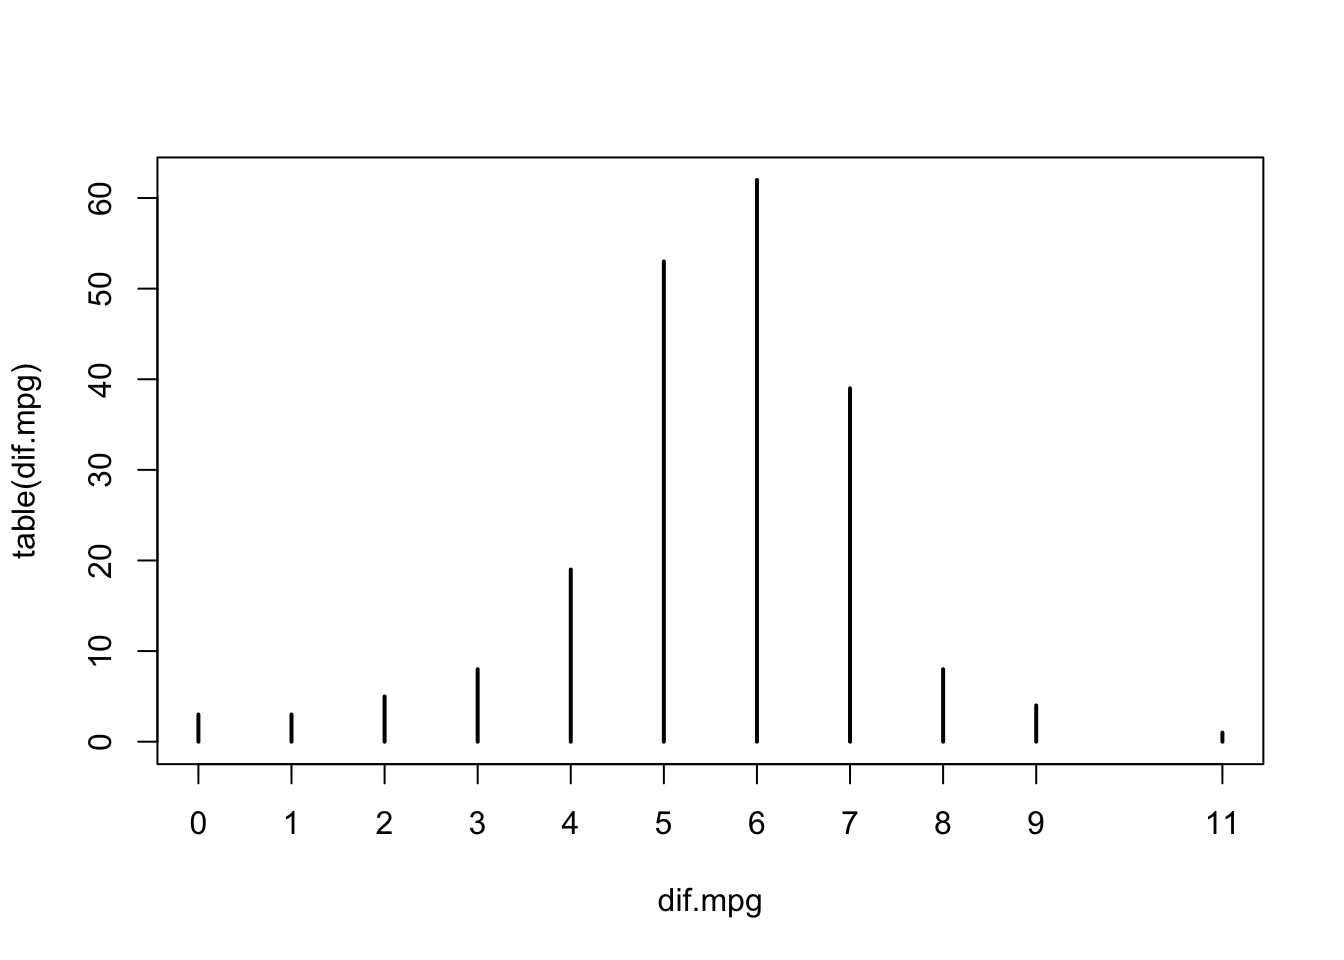
\includegraphics[width=0.6\linewidth]{statthink_files/figure-latex/unnamed-chunk-176-1} \end{center}

In the first expression we created the variable ``\texttt{dif.mpg}'' that
contains the difference in miles-per-gallon. The difference is computed
for each car type between highway driving conditions and urban driving
condition. The summary of this variable is produced in the second
expression. Observe that the values of the variable range between 0 and
11, with 50\% of the distribution concentrated between 5 and 7. The
median is 6 and the mean is 5.532. The last expression produces the bar
plot of the distribution. It turns out that the variable ``\texttt{dif.mpg}''
obtains integer values.

In this section we test hypotheses regarding the expected difference in
fuel consumption between highway and city conditions.

Energy is required in order to move cars. For heavier cars more energy
is required. Consequently, one may conjecture that milage per gallon for
heavier cars is less than the milage per gallon for lighter cars.

The relation between the weight of the car and the difference between
the milage-per-gallon in highway and city driving conditions is less
clear. On the one hand, urban traffic involves frequent changes in speed
in comparison to highway conditions. One may presume that this change in
speed is a cause for reduced efficiency in fuel consumption. If this is
the case then one may predict that heavier cars, which require more
energy for acceleration, will be associated with a bigger difference
between highway and city driving conditions in comparison to lighter
cars.

One the other hand, heavier cars do less miles per gallon overall. The
difference between two smaller numbers (the milage per gallon in highway
and in city conditions for heavier cars) may tend to be smaller than the
difference between two larger numbers (the milage per gallon in highway
and in city conditions for lighter cars). If this is the case then one
may predict that heavier cars will be associated with a smaller
difference between highway and city driving conditions in comparison to
lighter cars.

The average difference between highway and city conditions is
approximately 5.53 for all cars. Divide the cars into to two groups of
equal size: One group is composed of the heavier cars and the other
group is composed of the lighter cars. We will examine the relation
between the weight of the car and difference in miles per gallon between
the two driving conditions by testing hypotheses separately for each
weight group\footnote{In the next chapters we will consider a more direct ways for
  comparing the effect of one variable (\texttt{curb.weight} in this example)
  on the distribution of another variable (\texttt{dif.mpg} in this example).
  Here, instead, we investigate the effect indirectly by the
  investigation of hypotheses on the expectation of the variable
  \texttt{dif.mpg} separately for heavier cars and for lighter cars.}. For each such group we start by testing the two-sided
hypothesis \(H_1:\Expec(X) \not = 5.53\), where \(X\) is the difference
between highway and city miles-per-gallon in cars that belong to the
given weight group. After carrying the test for the two-sided
alternative we will discuss results of the application of tests for
one-sided alternatives.

We start by the definition of the weight groups. The variable
``\texttt{curb.weight}'' measures the weight of the cars in the data frame
``\texttt{cars}''. Let us examine the summary of the content of this variable:

\begin{Shaded}
\begin{Highlighting}[]
\KeywordTok{summary}\NormalTok{(cars}\OperatorTok{$}\NormalTok{curb.weight)}
\end{Highlighting}
\end{Shaded}

\begin{verbatim}
##    Min. 1st Qu.  Median    Mean 3rd Qu.    Max. 
##  1488.0  2145.0  2414.0  2555.6  2935.0  4066.0
\end{verbatim}

Half of the cars in the data frame weigh less than 2,414 lb and half the
cars weigh more. The average weight of a car is 2,556 lb. Let us take
2,414 as a threshold and denote cars below this weight as ``light'' and
cars above this threshold as ``heavy'':

\begin{Shaded}
\begin{Highlighting}[]
\NormalTok{heavy <-}\StringTok{ }\NormalTok{cars}\OperatorTok{$}\NormalTok{curb.weight }\OperatorTok{>}\StringTok{ }\DecValTok{2414}
\KeywordTok{table}\NormalTok{(heavy)}
\end{Highlighting}
\end{Shaded}

\begin{verbatim}
## heavy
## FALSE  TRUE 
##   103   102
\end{verbatim}

The variable ``\texttt{heavy}'' indicates for each car type whether its weight is
above or below the threshold weight of 2,414 lb. The variable is
composed of a sequence with as many components as the number of
observations in the data frame ``\texttt{cars}'' (\(n = 205\)). Each component is a
logical value: ``\texttt{TRUE}'' if the car is heavier than the threshold and
``\texttt{FALSE}'' if it is not. When we apply the function ``\texttt{table}'' to this
sequence we get that 102 of the cars are heavier than the threshold and
103 are not so.

We would like to apply the \(t\)-test first to the subset of all cars with
weight above 2,414 lb (cars that are associated with the value ``\texttt{TRUE}''
in the variable ``\texttt{heavy}''), and then to all cars with weights not
exceeding the threshold (cars associated with value ``\texttt{FALSE}''). In the
past we showed that one may address components of a sequence using its
position in the sequence\footnote{For example, in Question~\[ex:Inference.1\] we referred to the
  first 29 observations of the sequence ``\texttt{change}'' using the
  expression ``\texttt{change{[}1:29{]}}'' and to the last 21 observations using
  the expression ``\texttt{change{[}30:50{]}}''.}. Here we demonstrate an alternative
approach for addressing specific locations by using a sequence with
logical components.

In order to illustrate this second approach consider the two sequences:

\begin{Shaded}
\begin{Highlighting}[]
\NormalTok{w <-}\StringTok{ }\KeywordTok{c}\NormalTok{(}\DecValTok{5}\NormalTok{,}\DecValTok{3}\NormalTok{,}\DecValTok{4}\NormalTok{,}\DecValTok{6}\NormalTok{,}\DecValTok{2}\NormalTok{,}\DecValTok{9}\NormalTok{)}
\NormalTok{d <-}\StringTok{ }\KeywordTok{c}\NormalTok{(}\DecValTok{13}\NormalTok{,}\DecValTok{22}\NormalTok{,}\DecValTok{0}\NormalTok{,}\DecValTok{12}\NormalTok{,}\DecValTok{6}\NormalTok{,}\DecValTok{20}\NormalTok{)}
\end{Highlighting}
\end{Shaded}

Say we want to select the components of the sequence ``\texttt{d}'' in all the
locations where the components of the sequence ``\texttt{w}'' obtain values
larger than 5. Consider the code:

\begin{Shaded}
\begin{Highlighting}[]
\NormalTok{w }\OperatorTok{>}\StringTok{ }\DecValTok{5}
\end{Highlighting}
\end{Shaded}

\begin{verbatim}
## [1] FALSE FALSE FALSE  TRUE FALSE  TRUE
\end{verbatim}

\begin{Shaded}
\begin{Highlighting}[]
\NormalTok{d[w }\OperatorTok{>}\StringTok{ }\DecValTok{5}\NormalTok{]}
\end{Highlighting}
\end{Shaded}

\begin{verbatim}
## [1] 12 20
\end{verbatim}

The expression ``\texttt{w\ \textgreater{}\ 5}'' is a sequence of logical components, with the
value ``\texttt{TRUE}'' at the positions where ``\texttt{w}'' is above the threshold and
the value ``\texttt{FALSE}'' at the positions where ``\texttt{w}'' is below the threshold.
We may use the sequence with logical components as an index to the
sequence of the same length ``\texttt{d}''. The relevant expression is
``\texttt{d{[}w\ \textgreater{}\ 5{]}}''. The output of this expression is the sub-sequence of
elements from ``\texttt{d}'' that are associated with the ``\texttt{TRUE}'' values of the
logical sequence. Indeed, ``\texttt{TRUE}'' values are present at the 4th and the
6th positions of the logical sequence. Consequently, the output of the
expression ``\texttt{d{[}w\ \textgreater{}\ 5{]}}'' contains the 4th and the 6th components of the
sequence ``\texttt{d}''.

The operator ``\texttt{!}'', when applied to a logical value, reverses the value.
A ``\texttt{TRUE}'' becomes ``\texttt{FALSE}'' and a ``\texttt{FALSE}'' becomes ``\texttt{TRUE}''. Consider
the code:

\begin{Shaded}
\begin{Highlighting}[]
\OperatorTok{!}\NormalTok{(w }\OperatorTok{>}\StringTok{ }\DecValTok{5}\NormalTok{)}
\end{Highlighting}
\end{Shaded}

\begin{verbatim}
## [1]  TRUE  TRUE  TRUE FALSE  TRUE FALSE
\end{verbatim}

\begin{Shaded}
\begin{Highlighting}[]
\NormalTok{d[}\OperatorTok{!}\NormalTok{(w }\OperatorTok{>}\StringTok{ }\DecValTok{5}\NormalTok{)]}
\end{Highlighting}
\end{Shaded}

\begin{verbatim}
## [1] 13 22  0  6
\end{verbatim}

Observe that the sequence ``\texttt{!(w\ \textgreater{}\ 5)}'' obtains a value of ``\texttt{TRUE}'' at
the positions where ``\texttt{w}'' is less or equal to 5. Consequently, the
output of the expression ``\texttt{d{[}!(w\ \textgreater{}\ 5){]}}'' are all the values of ``\texttt{d}''
that are associated with components of ``\texttt{w}'' that are less or equal to
5.

The variable ``\texttt{dif.mpg}'' contains data on the difference in
miles-per-gallon between highway and city driving conditions for all the
car types. The sequence ``\texttt{heavy}'' identifies the car types with curb
weight above the threshold of 2,414 lb. The components of this sequence
are logical with the value ``\texttt{TRUE}'' at positions associated with the
heavier car types and the ``\texttt{FALSE}'' at positions associated with the
lighter car types. Observe that the output of the expression
``\texttt{dif.mpg{[}heavy{]}}'' is the subsequence of differences in miles-per-gallon
for the cars with curb weight above the given threshold. We apply the
function ``\texttt{t.test}'' to this expression in order to conduct the \(t\)-test
on the expectation of the variable ``\texttt{dif.mpg}'' for the heavier cars:

\begin{Shaded}
\begin{Highlighting}[]
\KeywordTok{t.test}\NormalTok{(dif.mpg[heavy],}\DataTypeTok{mu=}\FloatTok{5.53}\NormalTok{)}
\end{Highlighting}
\end{Shaded}

\begin{verbatim}
## 
##  One Sample t-test
## 
## data:  dif.mpg[heavy]
## t = -1.53853, df = 101, p-value = 0.12705
## alternative hypothesis: true mean is not equal to 5.53
## 95 percent confidence interval:
##  4.9001983 5.6096057
## sample estimates:
## mean of x 
##  5.254902
\end{verbatim}

The target population are the heavier car types. Notice that we test the
null hypothesis that expected difference among he heavier cars is equal
to 5.53 against the alternative hypothesis that the expected difference
among heavier cars is not equal to 5.53. The null hypothesis is not
rejected at the 5\% significance level since the \(p\)-value, which is
equal to 0.1735, is larger than 0.05. Consequently, based on the data at
hand, we cannot conclude that the expected difference in
miles-per-gallon for heavier cars is significantly different than the
average difference for all cars.

Observe also that the estimate of the expectation, the sample mean, is
equal to 5.254902, with a confidence interval of the form
\([4.900198, 5.609606]\).

Next, let us apply the same test to the lighter cars. The expression
``\texttt{dif.pmg{[}!heavy{]}}'' produces the subsequence of differences in
miles-per-gallon for the cars with curb weight below the given
threshold. The application of the function ``\texttt{t.test}'' to this
subsequence gives:

\begin{Shaded}
\begin{Highlighting}[]
\KeywordTok{t.test}\NormalTok{(dif.mpg[}\OperatorTok{!}\NormalTok{heavy],}\DataTypeTok{mu=}\FloatTok{5.53}\NormalTok{)}
\end{Highlighting}
\end{Shaded}

\begin{verbatim}
## 
##  One Sample t-test
## 
## data:  dif.mpg[!heavy]
## t = 1.96923, df = 102, p-value = 0.051639
## alternative hypothesis: true mean is not equal to 5.53
## 95 percent confidence interval:
##  5.5280018 6.0836487
## sample estimates:
## mean of x 
## 5.8058252
\end{verbatim}

Again, the null hypothesis is not rejected at the 5\% significance level
since a \(p\)-value of 0.05164 is still larger than 0.05. However, unlike
the case for heavier cars where the \(p\)-value was undeniably larger than
the threshold. In this example it is much closer to the threshold of
0.05. Consequently, we may almost conclude that the expected difference
in miles-per-gallon for lighter cars is significantly different than the
average difference for all car.

Why did we not reject the null hypothesis for the heavier cars but
almost did so for the lighter cars? Both tests are based on the \(T\)
statistic, which measures the ratio between the deviation of the sample
average from its expectation under the null, divided by the estimate of
the standard deviation of the sample average. The value of this
statistic is ``\texttt{t\ =\ -1.5385}'' for heavier cars and it is ``\texttt{t\ =\ 1.9692}''
for lighter cars, an absolute value of about 25\% higher.

The deviation of the sample average for the heavier cars and the
expectation under the null is \(5.254902 - 5.53 = -0.275098\). On the
other hand, the deviation of the sample average for the lighter cars and
the expectation under the null is \(5.805825 - 5.53 = 0.275825\). The two
deviations are practically equal to each other in the absolute value.

The estimator of the standard deviation of the sample average is
\(S/\sqrt{n}\), where \(S\) is the sample standard deviation and \(n\) is the
sample size. The sample sizes, 103 for lighter cars and 102 for heavier
cars, are almost equal. Therefore, the reason for the difference in the
values of the \(T\) statistics for both weight groups must be differences
in the sample standard deviations. Indeed, when we compute the sample
standard deviation for lighter and heavier cars\footnote{The function ``\texttt{tapply}'' applies the function that is given as its
  third argument (the function ``\texttt{sd}'' in this case) to each subset of
  values of the sequence that is given as its first argument (the
  sequence ``\texttt{dif.mpg}'' in the current application). The subsets are
  determined by the levels of the second arguments (the sequence
  ``\texttt{heavy}'' in this case). The output is the sample standard deviation
  of the variable ``\texttt{dif.mpg}'' for lighter cars (the level ``\texttt{FALSE}'')
  and for heavier cars (the level ``\texttt{TRUE}'').} we get that the
standard deviation for lighter cars (1.421531) is much smaller than the
standard deviation for heavier cars (1.805856):

\begin{Shaded}
\begin{Highlighting}[]
\KeywordTok{tapply}\NormalTok{(dif.mpg,heavy,sd)}
\end{Highlighting}
\end{Shaded}

\begin{verbatim}
##     FALSE      TRUE 
## 1.4215309 1.8058556
\end{verbatim}

The important lesson to learn from this exercise is that simple minded
notion of significance and statistical significance are not the same. A
simple minded assessment of the discrepancy from the null hypothesis
will put the evidence from the data on lighter cars and the evidence
from the data on heavier cars on the same level. In both cases the
estimated value of the expectation is the same distance away from the
null value.

However, statistical assessment conducts the analysis in the context of
the sampling distribution. The deviation of the sample average from the
expectation is compared to the standard deviation of the sample average.
Consequently, in statistical testing of hypothesis a smaller deviation
of the sample average from the expectation under the null may be more
significant than a larger one if the sampling variability of the former
is much smaller than the sampling variability of the later.

Let us proceed with the demonstration of the application of the \(t\)-test
by the testing of one-sided alternatives in the context of the lighter
cars. One may test the one-sided alternative \(H_1:\Expec(X) > 5.53\) that
the expected value of the difference in miles-per-gallon among cars with
curb weight no more than 2,414 lb is \emph{greater} than 5.53 by the
application of the function ``\texttt{t.test}'' to the data on lighter cars. This
data is the output of the expression ``\texttt{dif.mpg{[}!heavy{]}}''. As before, we
specify the null value of the expectation by the introduction of the
expression ``\texttt{mu=5.53}''. The fact that we are interested in the testing
of the specific alternative is specified by the introduction of a new
argument of the form: ``\texttt{alternative=greater}''. The default value of the
argument ``\texttt{alternative}'' is ``\texttt{two.sided}'', which produces a test of a
two-sided alternative. By changing the value of the argument to
``\texttt{greater}'' we produce a test for the appropriate one-sided alternative:

\begin{Shaded}
\begin{Highlighting}[]
\KeywordTok{t.test}\NormalTok{(dif.mpg[}\OperatorTok{!}\NormalTok{heavy],}\DataTypeTok{mu=}\FloatTok{5.53}\NormalTok{,}\DataTypeTok{alternative=}\StringTok{"greater"}\NormalTok{)}
\end{Highlighting}
\end{Shaded}

\begin{verbatim}
## 
##  One Sample t-test
## 
## data:  dif.mpg[!heavy]
## t = 1.96923, df = 102, p-value = 0.02582
## alternative hypothesis: true mean is greater than 5.53
## 95 percent confidence interval:
##  5.5733228       Inf
## sample estimates:
## mean of x 
## 5.8058252
\end{verbatim}

The value of the test statistic (\texttt{t\ =\ 1.9692}) is the same as for the
test of the two-sided alternative and so is the number of degrees of
freedom associated with the statistic (\texttt{df\ =\ 102}). However, the
\(p\)-value is smaller (\texttt{p-value\ =\ 0.02582}), compared to the \(p\)-value in
the test for the two-sided alternative (\texttt{p-value\ =\ 0.05164}). The
\(p\)-value for the one-sided test is the probability under the sampling
distribution that the test statistic obtains vales larger than the
observed value of 1.9692. The \(p\)-value for the two-sided test is twice
that figure since it involves also the probability of being less than
the negative of the observes value.

The estimated value of the expectation, the sample average, is
unchanged. However, instead of producing a confidence interval for the
expectation the report produces a \emph{one-sided} confidence interval of the
form \([5.573323, \infty)\). Such an interval corresponds to the
\emph{smallest} value that the expectation may reasonably obtain on the basis
of the observed data.

Finally, consider the test of the other one-sided alternative
\(H_1:\Expec(X) < 5.53\):

\begin{Shaded}
\begin{Highlighting}[]
\KeywordTok{t.test}\NormalTok{(dif.mpg[}\OperatorTok{!}\NormalTok{heavy],}\DataTypeTok{mu=}\FloatTok{5.53}\NormalTok{,}\DataTypeTok{alternative=}\StringTok{"less"}\NormalTok{)}
\end{Highlighting}
\end{Shaded}

\begin{verbatim}
## 
##  One Sample t-test
## 
## data:  dif.mpg[!heavy]
## t = 1.96923, df = 102, p-value = 0.97418
## alternative hypothesis: true mean is less than 5.53
## 95 percent confidence interval:
##       -Inf 6.0383277
## sample estimates:
## mean of x 
## 5.8058252
\end{verbatim}

The alternative here is determined by the expression
``\texttt{alternative=less}''. The \(p\)-value is equal to 0.9742, which is the
probability that the test statistic obtains values less than the
observed value of 1.9692. Clearly, the null hypothesis is not rejected
in this test.

\hypertarget{TestFrac}{%
\section{Testing Hypothesis on Proportion}\label{TestFrac}}

Consider the problem of testing hypothesis on the probability of an
event. Recall that a probability \(p\) of some event can be estimated by
the observed relative frequency of the event in the sample, denoted
\(\hat P\). The estimation is associated with the Bernoulli random
variable \(X\), that obtains the value 1 when the event occurs and the
value 0 when it does not. The statistical model states that \(p\) is the
expectation of \(X\). The estimator \(\hat P\) is the sample average of this
measurement.

With this formulation we may relate the problem of testing hypotheses
formulated in terms of \(p\) to the problem of tests associated to the
expectation of a measurement. For the latter problem we applied the
\(t\)-test. A similar, though not identical, test is used for the problem
of testing hypothesis on proportions.

Assume that one in interested in testing the null hypothesis that the
probability of the event is equal to some specific value, say one half,
versus the alternative hypothesis that the probability is not equal to
this value. These hypotheses are formulated as \(H_0:p = 0.5\) and
\(H_1:p\not = 0.5\).

The sample proportion of the event \(\hat P\) is the basis for the
construction of the test statistic. Recall that the variance of the
estimator \(\hat P\) is given by \(\Var(\hat P) = p(1-p)/n\). Under the null
hypothesis we get that the variance is equal to
\(\Var(\hat P) = 0.5(1-0.5)/n\). A natural test statistic is the
standardized sample proportion:

\[Z = \frac{\hat P - 0.5}{\sqrt{0.5 (1-0.5)/n}}\;,\] that measures the
ratio between the deviation of the estimator from its null expected
value and the standard deviation of the estimator. The standard
deviation of the sample proportion is used in the ratio.

If the null hypothesis that \(p=0.5\) holds true then one gets that the
value 0 is the center of the sampling distribution of the test statistic
\(Z\). Values of the statistic that are much larger or much smaller than 0
indicate that the null hypothesis is unlikely. Consequently, one may
consider a rejection region of the form \(\{|Z| > c\}\), for some
threshold value \(c\). The threshold \(c\) is set at a high enough level to
assure the required significance level, namely the probability under the
null hypothesis of obtaining a value in the rejection region.
Equivalently, the rejection region can be written in the form
\(\{Z^2 > c^2\}\).

As a result of the Central Limit Theorem one may conclude that the
distribution of the test statistic is approximately Normal. Hence,
Normal computations may be used in order to produce an approximate
threshold or in order to compute an approximation for the \(p\)-value.
Specifically, if \(Z\) has the standard Normal distribution then \(Z^2\) has
a chi-square distribution on one degree of freedom.

In order to illustrate the application of hypothesis testing for
proportion consider the following problem: In the previous section we
obtained the curb weight of 2,414 lb as the sample median. The weights
of half the cars in the sample were above that level and the weights of
half the cars were below this level. If this level was actually the
population median then the probability that the weight of a random car
is not exceeding this level would be equal to 0.5.

Let us test the hypothesis that the median weight of cars that run on
diesel is also 2,414 lb. Recall that 20 out of the 205 car types in the
sample have diesel engines. Let us use the weights of these cars in
order to test the hypothesis.

The variable ``\texttt{fuel.type}'' is a factor with two levels ``\texttt{diesel}'' and
``\texttt{gas}'' that identify the fuel type of each car. The variable ``\texttt{heavy}''
identifies for each car whether its weight is above the level of 2414 or
not. Let us produce a \(2 \times 2\) table that summarizes the frequency
of each combination of weight group and the fuel type:

\begin{Shaded}
\begin{Highlighting}[]
\NormalTok{fuel <-}\StringTok{ }\NormalTok{cars}\OperatorTok{$}\NormalTok{fuel.type}
\KeywordTok{table}\NormalTok{(fuel,heavy)}
\end{Highlighting}
\end{Shaded}

\begin{verbatim}
##         heavy
## fuel     FALSE TRUE
##   diesel     6   14
##   gas       97   88
\end{verbatim}

Originally the function ``\texttt{table}'' was applied to a single factor and
produced a sequence with the frequencies of each level of the factor. In
the current application the input to the function are two factors\footnote{To be more accurate, the variable ``\texttt{heavy}'' is not a factor but a
  sequence with logical components. Nonetheless, when the function
  ``\texttt{table}'' is applied to such a sequence it treats it as a factor
  with two levels, ``\texttt{TRUE}'' and ``\texttt{FALSE}''.}.
The output is a table of frequencies. Each entry to the table
corresponds to the frequency of a combination of levels, one from the
first input factor and the other from the second input factor. In this
example we obtain that 6 cars use diesel and their curb weight was below
the threshold. There are 14 cars that use diesel and their curb weight
is above the threshold. Likewise, there are 97 light cars that use gas
and 88 heavy cars with gas engines.

The function ``\texttt{prop.test}'' produces statistical tests for proportions.
The relevant information for the current application of the function is
the fact that frequency of light diesel cars is 6 among a total number
of 20 diesel cars. The first entry to the function is the frequency of
the occurrence of the event, 6 in this case, and the second entry is the
relevant sample size, the total number of diesel cars which is 20 in the
current example:

\begin{Shaded}
\begin{Highlighting}[]
\KeywordTok{prop.test}\NormalTok{(}\DecValTok{6}\NormalTok{,}\DecValTok{20}\NormalTok{)}
\end{Highlighting}
\end{Shaded}

\begin{verbatim}
## 
##  1-sample proportions test with continuity correction
## 
## data:  6 out of 20, null probability 0.5
## X-squared = 2.45, df = 1, p-value = 0.11752
## alternative hypothesis: true p is not equal to 0.5
## 95 percent confidence interval:
##  0.12839086 0.54330713
## sample estimates:
##   p 
## 0.3
\end{verbatim}

The function produces a report that is printed on the screen. The title
identifies the test as a one-sample test of proportions. In later
chapters we will apply the same function to more complex data structures
and the title will change accordingly. The title also identifies the
fact that a continuity correction is used in the computation of the test
statistic.

The line under the title indicates the frequency of the event in the
sample and the sample size. (In the current example, 6 diesel cars with
weights below the threshold among a total of 20 diesel cars.) The
probability of the event, under the null hypothesis, is described. The
default value of this probability is ``\texttt{p\ =\ 0.5}'', which is the proper
value in the current example. This default value can be modified by
replacing the value 0.5 by the appropriate probability.

The next line presents the information relevant for the test itself. The
test statistic, which is essentially the square of the \(Z\) statistic
described above\footnote{The test statistic that is computed by default is based on
  \emph{Yates' correction for continuity}, which is very similar to the
  continuity correction that was used in Chapter~\[ch:Normal\] for the
  Normal approximation of the Binomial distribution. Specifically, the
  test statistic to the continuity correction for testing
  \(H_0:p = p_0\) takes the form
  \([|\hat p - p_0|-0.5/n]^2/[p_0(1-p_0)/n]\). Compare this statistic
  with the statistic proposed in the text that takes the form
  \([\hat p - p_0]^2/[p_0(1-p_0)/n]\). The latter statistic is used if
  the argument ``\texttt{correct\ =\ FALSE}'' is added to the function.}, obtains the value 2.45. The sampling distribution
of this statistic under the null hypothesis is, approximately, the
chi-square distribution on 1 degree of freedom. The \(p\)-value, which is
the probability that chi-square distribution on 1 degree of freedom
obtains a value above 2.45, is equal to 0.1175. Consequently, the null
hypothesis is not rejected at the 5\% significance level.

The bottom part of the report provides the confidence interval and the
point estimate for the probability of the event. The confidence interval
for the given data is \([0.1283909, 0.5433071]\) and the point estimate is
\(\hat p = 6/20 = 0.3\).

It is interesting to note that although the deviation between the
estimated proportion \(\hat p = 0.3\) and the null value of the
probability \(p = 0.5\) is relatively large still the null hypothesis was
not rejected. The reason for that is the smallness of the sample,
\(n = 20\), that was used in order to test the hypothesis. Indeed, as an
exercise let us examine the application of the same test to a setting
where \(n = 200\) and the number of occurrences of the event is 60:

\begin{Shaded}
\begin{Highlighting}[]
\KeywordTok{prop.test}\NormalTok{(}\DecValTok{60}\NormalTok{,}\DecValTok{200}\NormalTok{)}
\end{Highlighting}
\end{Shaded}

\begin{verbatim}
## 
##  1-sample proportions test with continuity correction
## 
## data:  60 out of 200, null probability 0.5
## X-squared = 31.205, df = 1, p-value = 2.3217e-08
## alternative hypothesis: true p is not equal to 0.5
## 95 percent confidence interval:
##  0.23844235 0.36938918
## sample estimates:
##   p 
## 0.3
\end{verbatim}

The estimated value of the probability is the same as before since
\(\hat p = 60/200 = 0.3\). However, the \(p\)-value is
\(2.322 \times 10^{-8}\), which is way below the significance threshold of
0.05. In this scenario the null hypothesis is rejected with flying
colors.

This last example is yet another demonstration of the basic
characteristic of statistical hypothesis testing. The consideration is
based not on the discrepancy of the estimator of the parameter from the
value of the parameter under the null. Instead, it is based on the
\emph{relative} discrepancy in comparison to the sampling variability of the
estimator. When the sample size is larger the variability is smaller.
Hence, the chances of rejecting the null hypothesis for the same
discrepancy increases.

\hypertarget{exercises-7}{%
\section{Exercises}\label{exercises-7}}

\BeginKnitrBlock{exercise}
\protect\hypertarget{exr:unnamed-chunk-190}{}{\label{exr:unnamed-chunk-190} }Consider a medical condition that does not have a
standard treatment. The recommended design of a clinical trial for a new
treatment to such condition involves using a placebo treatment as a
control. A placebo treatment is a treatment that externally looks
identical to the actual treatment but, in reality, it does not have the
active ingredients. The reason for using placebo for control is the
``placebo effect''. Patients tent to react to the fact that they are being
treated regardless of the actual beneficial effect of the treatment.

As an example, consider the trial for testing magnets as a treatment for
pain that was described in Question~\[ex:Inference.1\]. The patients
that where randomly assigned to the control (the last 21 observations in
the file ``\texttt{magnets.csv}'') were treated with devises that looked like
magnets but actually were not. The goal in this exercise is to test for
the presence of a placebo effect in the case study ``Magnets and Pain
Relief'' of Question~\[ex:Inference.1\] using the data in the file
``\texttt{magnets.csv}''.

\begin{enumerate}
\def\labelenumi{\arabic{enumi}.}
\item
  Let \(X\) be the measurement of change, the difference between the
  score of pain before the treatment and the score after the
  treatment, for patients that were treated with the inactive placebo.
  Express, in terms of the expected value of \(X\), the null hypothesis
  and the alternative hypothesis for a statistical test to determine
  the presence of a placebo effect. The null hypothesis should reflect
  the situation that the placebo effect is absent.
\item
  Identify the observations that can be used in order to test the
  hypotheses.
\item
  Carry out the test and report your conclusion. (Use a significance
  level of 5\%.)
\end{enumerate}
\EndKnitrBlock{exercise}

\BeginKnitrBlock{exercise}
\protect\hypertarget{exr:unnamed-chunk-191}{}{\label{exr:unnamed-chunk-191} }It is assumed, when constructing the \(t\)-test, that the
measurements are Normally distributed. In this exercise we examine the
robustness of the test to divergence from the assumption. You are
required to compute the significance level of a two-sided \(t\)-test of
\(H_0:\Expec(X)=4\) versus \(H_1: \Expec(X) \not = 4\). Assume there are
\(n=20\) observations and use a \(t\)-test with a nominal 5\% significance
level.

\begin{enumerate}
\def\labelenumi{\arabic{enumi}.}
\item
  Consider the case where \(X \sim \mathrm{Exponential}(1/4)\).
\item
  Consider the case where \(X \sim \mathrm{Uniform}(0,8)\).
\end{enumerate}
\EndKnitrBlock{exercise}

\BeginKnitrBlock{exercise}
\protect\hypertarget{exr:unnamed-chunk-192}{}{\label{exr:unnamed-chunk-192} }Assume that you are interested in testing
\(H_0:\Expec(X) = 20\) versus \(H_1:\Expec(X)\not = 20\) with a significance
level of 5\% using the \(t\)-test. Let the sample average, of a sample of
size \(n=55\), be equal to \(\bar x = 22.7\) and the sample standard
deviation be equal to \(s = 5.4\).

\begin{enumerate}
\def\labelenumi{\arabic{enumi}.}
\item
  Do you reject the null hypothesis?
\item
  Use the same information. Only now you are interested in a
  significance level of 1\%. Do you reject the null hypothesis?
\item
  Use the information the presentation of the exercise. But now you
  are interested in testing \(H_0:\Expec(X) = 24\) versus
  \(H_1:\Expec(X)\not = 24\) (with a significance level of 5\%). Do you
  reject the null hypothesis?
\end{enumerate}
\EndKnitrBlock{exercise}

\hypertarget{summary-10}{%
\section{Summary}\label{summary-10}}

\hypertarget{glossary}{%
\subsection*{Glossary}\label{glossary}}


\begin{description}
\item[Hypothesis Testing:]
A method for determining between two hypothesis, with one of the two
being the currently accepted hypothesis. A determination is based on
the value of the test statistic. The probability of falsely
rejecting the currently accepted hypothesis is the significance
level of the test.
\item[Null Hypothesis (\(H_0\)):]
A sub-collection that emerges in response to the situation when the
phenomena is absent. The established scientific theory that is being
challenged. The hypothesis which is worse to erroneously reject.
\item[Alternative Hypothesis (\(H_1\)):]
A sub-collection that emerges in response to the presence of the
investigated phenomena. The new scientific theory that challenges
the currently established theory.
\item[Test Statistic:]
A statistic that summarizes the data in the sample in order to
decide between the two alternative.
\item[Rejection Region:]
A set of values that the test statistic may obtain. If the observed
value of the test statistic belongs to the rejection region then the
null hypothesis is rejected. Otherwise, the null hypothesis is not
rejected.
\item[Type I Error]
The null hypothesis is correct but it is rejected by the test.
\item[Type II Error]
The alternative hypothesis holds but the null hypothesis is not
rejected by the test.
\item[Significance Level:]
The probability of a Type I error. The probability, computed under
the null hypothesis, of rejecting the null hypothesis. The test is
constructed to have a given significance level. A commonly used
significance level is 5\%.
\item[Statistical Power:]
The probability, computed under the alternative hypothesis, of
rejecting the null hypothesis. The statistical power is equal to 1
minus the probability of a Type II error.
\item[\(p\)-value:]
A form of a test statistic. It is associated with a specific test
statistic and a structure of the rejection region. The \(p\)-value is
equal to the significance level of the test in which the observed
value of the statistic serves as the threshold.
\end{description}

\hypertarget{discuss-in-the-forum}{%
\subsection*{Discuss in the forum}\label{discuss-in-the-forum}}


In statistical thinking there is a tenancy towards conservatism. The
investigators, enthusiastic to obtain positive results, may prefer
favorable conclusions and may tend over-interpret the data. It is the
statistician's role to add to the objectivity in the interpretation of
the data and to advocate caution.

On the other hand, the investigators may say that conservatism and
science are incompatible. If one is too cautious, if one is always
protecting oneself against the worst-case scenario, then one will not be
able to make bold new discoveries.

Which of the two approach do you prefer?

When you formulate your answer to this question it may be useful to
recall cases in your past in which you where required to analyze data or
you were exposed to other people's analysis. Could the analysis benefit
or be harmed by either of the approaches?

For example, many scientific journal will tend to reject a research
paper unless the main discoveries are statistically significant
(\(p\)-value \(<\) 5\%). Should one not publish also results that show a
significance level of 10\%?

\hypertarget{formulas}{%
\subsection*{Formulas:}\label{formulas}}


\begin{itemize}
\item
  Test Statistic for Expectation:
  \(t = (\bar x - \mu_0)/ (s/\sqrt{n})\).
\item
  Two-Sided Test: Reject \(H_0\) if
  \(\{|t| > \mbox{\texttt{qt(0.975,n-1)}}\}\).
\item
  Greater Than: Reject \(H_0\) if
  \(\{t > \mbox{\texttt{qt(0.95,n-1)}}\}\).
\item
  Less Than: Reject \(H_0\) if \(\{t < \mbox{\texttt{qt(0.05,n-1)}}\}\).
\end{itemize}

\hypertarget{ChapTwoSamp}{%
\chapter{Comparing Two Samples}\label{ChapTwoSamp}}

\hypertarget{student-learning-objectives-7}{%
\section{Student Learning Objectives}\label{student-learning-objectives-7}}

The next 3 chapters deal with the statistical inference associated with
the relation between two variables. The relation corresponds to the
effect of one variable on the distribution of the other. The variable
whose distribution is being investigated is called the \emph{response}. The
variable which may have an effect on the distribution of the response is
called the \emph{explanatory variable}.

In this section we consider the case where the explanatory variable is a
factor with two levels. This factor splits the sample into two
sub-samples. The statistical inference compares between the
distributions of the response variable in the two sub-samples. The
statistical inference involves point estimation, confidence intervals,
and hypothesis testing. \texttt{R} functions may be used in order to carry out
the statistical inference. By the end of this chapter, the student
should be able to:

\begin{itemize}
\item
  Define estimators, confidence intervals, and tests for comparing the
  distribution of a numerical response between two sub-populations.
\item
  Apply the function ``\texttt{t.test}'' in order to investigate the difference
  between the expectations of the response variable in the two
  sub-samples.
\item
  Apply the function ``\texttt{var.test}'' in order to investigate the ratio
  between the variances of the response variable in the two
  sub-samples.
\end{itemize}

\hypertarget{comparing-two-distributions}{%
\section{Comparing Two Distributions}\label{comparing-two-distributions}}

Up until this point in the book we have been considering tools for the
investigation of the characteristics of the distribution of a single
measurement. In most applications, however, one is more interested in
inference regarding the relationships between several measurements. In
particular, one may want to understand how the outcome of one
measurement effects the outcome of another measurement.

A common form of a mathematical relation between two variables is when
one of the variables is a function of the other. When such a relation
holds then the value of the first variably is determined by the value of
the second. However, in the statistical context relations between
variables are more complex. Typically, a statistical relation between
variables does not make one a direct function of the other. Instead, the
\emph{distribution} of values of one of the variables is affected by the
value of the other variable. For a given value of the second variable
the first variable may have one distribution, but for a different value
of the second variable the distribution of the first variable may be
different. In statistical terminology the second variable in this
setting is called an \emph{explanatory variable} and the first variable, with
a distribution affected by the second variable, is called the
\emph{response}.

As an illustration of the relation between the response and the
explanatory variable consider the following example. In a clinical
trial, which is a precondition for the marketing of a new medical
treatment, a group of patients is randomly divided into a \emph{treatment}
and a \emph{control} sub-groups. The new treatment is anonymously
administered to the treatment sub-group. At the same time, the patients
in the control sub-group obtain the currently standard treatment. The
new treatment passes the trial and is approved for marketing by the
Health Authorities only if the response to the medical intervention is
better for the treatment sub-group than it is for the control sub-group.
This treatment-control experimental design, in which a response is
measured under two experimental conditions, is used in many scientific
and industrial settings.

In the example of a clinical trial one may identify two variables. One
variable measures the response to the medical intervention for each
patient that participated in the trial. This variable is the response
variable, the distribution of which one seeks to investigate. The other
variable indicates to which sub-group, treatment or control, each
patient belongs. This variable is the explanatory variable. In the
setting of a clinical trial the explanatory variable is a factor with
two levels, ``treatment'' and ``control'', that splits the sample into two
sub-samples. The statistical inference compares the distribution of the
response variable among the patients in the treatment sub-sample to the
distribution of the response among the patients in the control
sub-group.

The analysis of experimental settings such as the treatment-control
trial ia a special case that involves the investigation of the effect an
explanatory variable may have on the response variable. In this special
case the explanatory variable is a factor with two distinct levels. Each
level of the factor is associate with a sub-sample, either treatment or
control. The analysis seeks to compare the distribution of the response
in one sub-sample with the distribution in the other sub-sample. If the
response is a numeric measurement then the analysis may take the form of
comparing the response's expectation in one sub-group to the expectation
in the other. Alternatively, the analysis may involve comparing the
variance. In a different case, if the response is the indicator of the
occurrence of an event then the analysis may compare two probabilities,
the probability of the event in the treatment group to the probability
of the same event in the control group.

In this chapter we deal with statistical inference that corresponds to
the comparison of the distribution of a numerical response variable
between two sub-groups that are determined by a factor. The inference
includes testing hypotheses, mainly the null hypothesis that the
distribution of the response is the same in both subgroups versus the
alternative hypothesis that the distribution is not the same. Another
element in the inference is point estimation and confidence intervals of
appropriate parameters.

In the next chapter we will consider the case where the explanatory
variable is numeric and in the subsequent chapter we describe the
inference that is used in the case that the response is the indicator of
the occurrence of an event.

\hypertarget{sec:ComparingMeans}{%
\section{Comparing the Sample Means}\label{sec:ComparingMeans}}

In this section we deal with the issue of statistical inference when
comparing the expectation of the response variable in two sub-samples.
The inference is used in order to address questions such as the equality
of the two expectations to each other and, in the case they are not
equal, the assessment of the difference between the expectations. For
the first question one may use statistical hypothesis testing and for
the assessment one may use point estimates and/or confidence intervals.

In the first subsection we provide an example of a test of the
hypothesis that the expectations are equal. A confidence interval for
the difference between expectations is given in the output of the report
of the {\texttt{R}} function that applies the test. The second subsection
considers the construction of the confidence interval and the third
subsection deals with the theory behind the statistical test.

\hypertarget{an-example-of-a-comparison-of-means}{%
\subsection{An Example of a Comparison of Means}\label{an-example-of-a-comparison-of-means}}

In order to illustrate the statistical inference that compars two
expectations let us return to an example that was considered in
Chapter~\ref{ChapTesting}. The response of interest is the difference in
miles-per-gallon between driving in highway conditions and driving in
city conditions. This response is produced as the difference between the
variable ``\texttt{cars\$highway.mpg}'' and the variable ``\texttt{cars\$city.mpg}''. It is
stored in the object ``\texttt{dif.mpg}'', which is a numerical sequence:

\begin{Shaded}
\begin{Highlighting}[]
\NormalTok{cars <-}\StringTok{ }\KeywordTok{read.csv}\NormalTok{(}\StringTok{"_data/cars.csv"}\NormalTok{)}
\NormalTok{dif.mpg <-}\StringTok{ }\NormalTok{cars}\OperatorTok{$}\NormalTok{highway.mpg }\OperatorTok{-}\StringTok{ }\NormalTok{cars}\OperatorTok{$}\NormalTok{city.mpg}
\end{Highlighting}
\end{Shaded}

The object ``\texttt{heavy}'' was defined in the previous chapter as a sequence
with logical components. A component had the value ``\texttt{TRUE}'' if the curb
weight of the car type associated with this component was above the
median level of 2,414 lb. The component obtained the value ``\texttt{FALSE}'' if
the curb weight did not exceed that level. The logical sequence
``\texttt{heavy}'' was used in order to select the subsequences associated with
each weight sub-group. Statistical inference was applied separately to
each subsequence.

In the current analysis we want to examine directly the relation between
the response variable ``\texttt{dif.mpg}'' and an explanatory factor variable
``\texttt{heavy}''. In order to do so we redefine the variable ``\texttt{heavy}'' to be a
factor:

\begin{Shaded}
\begin{Highlighting}[]
\NormalTok{heavy <-}\StringTok{ }\KeywordTok{factor}\NormalTok{(cars}\OperatorTok{$}\NormalTok{curb.weight }\OperatorTok{>}\StringTok{ }\DecValTok{2414}\NormalTok{)}
\end{Highlighting}
\end{Shaded}

The variable ``\texttt{curb.weight}'' is numeric and the expression
``\texttt{cars\$curb.weight\ \textgreater{}\ 2414}'' produces a sequence with logical ``\texttt{TRUE}'' or
``\texttt{FALSE}'' components. This sequence is not a factor. In order to produce
a factor we apply the function ``\texttt{factor}'' to the sequence. The function
``\texttt{factor}'' transforms its input into a factor. Specifically, the
application of this function to a sequence with logical components
produces a factor with two levels that are given the names ``\texttt{TRUE}'' and
``\texttt{FALSE}''\footnote{It should be noted that the redefined sequence ``\texttt{heavy}'' is no
  longer a sequence with logical components. It cannot be used, for
  example, as an index to another sequence in order to sellect the
  components that are associated with the ``\texttt{TRUE}'' logical value.}.

We want to examine the relation between the response variable
``\texttt{dif.mpg}'' and the explanatory factor ``\texttt{heavy}''. Towards that end we
produce a plot of the relation with the function ``\texttt{plot}'' and test for
the equality of the expectations of the response with the function
``\texttt{t.test}''. First the plot:

\begin{Shaded}
\begin{Highlighting}[]
\KeywordTok{plot}\NormalTok{(dif.mpg}\OperatorTok{~}\NormalTok{heavy)}
\end{Highlighting}
\end{Shaded}

\begin{center}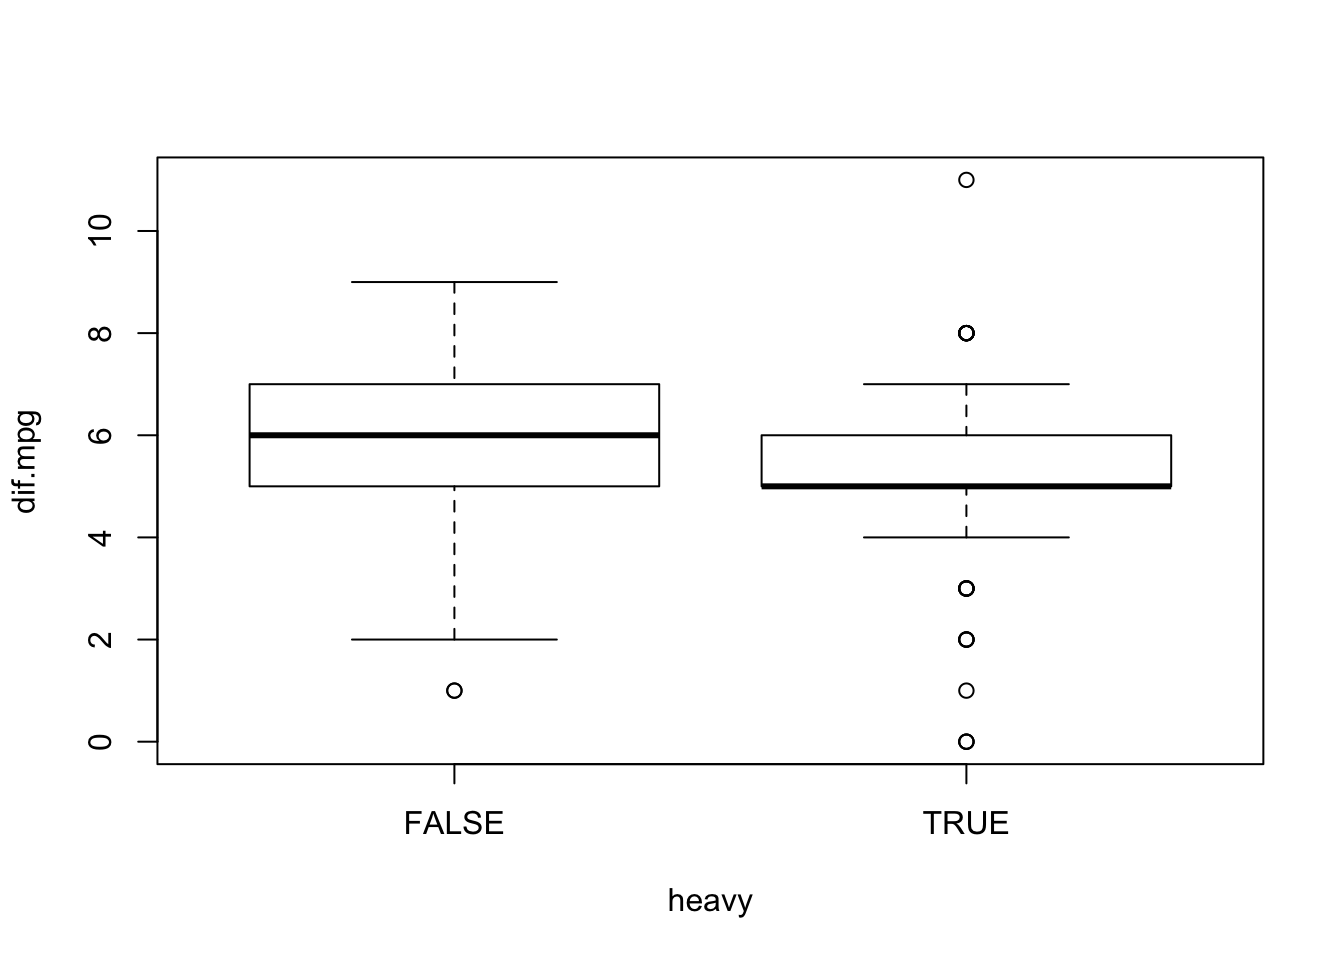
\includegraphics[width=0.6\linewidth]{statthink_files/figure-latex/unnamed-chunk-195-1} \end{center}

Observe that the figure contains two box plots, one associated with the
level ``\texttt{FALSE}'' of the explanatory factor and the other with the level
``\texttt{TRUE}'' of that factor. The box plots describe the distribution of the
response variable for each level of the explanatory factor. Overall, the
distribution of the response for heavier cars (cars associated with the
level ``\texttt{TRUE}'') tends to obtain smaller values than the distribution of
the response for lighter cars (cars associated with the level
``\texttt{FALSE}'').

The input to the function ``\texttt{plot}'' is a \emph{formula} expression of the
form: ``\emph{response\(\;\tilde{}\;\)explanatory.variable}''. A formula
identifies the role of variables. The variable to the left of the tilde
character (\(\;\tilde{}\;\)) in a formula is the response and the variable
to the right is the explanatory variable. In the current case the
variable ``\texttt{dif.mpg}'' is the response and the variable ``\texttt{heavy}'' is the
explanatory variable.

Let us use a formal test in order to negate the hypothesis that the
expectation of the response for the two weight groups is the same. The
test is provided by the application of the function ``\texttt{t.test}'' to the
formula ``\texttt{dif.mpg\textbackslash{};\textbackslash{}tilde\{\}\textbackslash{};heavy}'':

\begin{Shaded}
\begin{Highlighting}[]
\KeywordTok{t.test}\NormalTok{(dif.mpg}\OperatorTok{~}\NormalTok{heavy)}
\end{Highlighting}
\end{Shaded}

\begin{verbatim}
## 
##  Welch Two Sample t-test
## 
## data:  dif.mpg by heavy
## t = 2.42552, df = 191.561, p-value = 0.016214
## alternative hypothesis: true difference in means is not equal to 0
## 95 percent confidence interval:
##  0.10291504 0.99893152
## sample estimates:
## mean in group FALSE  mean in group TRUE 
##           5.8058252           5.2549020
\end{verbatim}

The function ``\texttt{t.test}'', when applied to a formula that describes the
relation between a numeric response and a explanatory factor with two
level, produces a special form of a \(t\)-test that is called the \emph{Welch
Two Sample \(t\)-test}. The statistical model associated with this test
assumes the present of two independent sub-samples, each associated with
a level of the explanatory variable. The relevant parameters for this
model are the two expectations and the two variances associated with the
sub-samples.

The hypotheses tested in the context of the Welch test are formulated in
terms of the difference between the expectation of the first sub-sample
and the expectation of the second sub-sample. In the default application
of the test the null hypothesis is that the difference is equal to 0
(or, equivalently, that the expectations are equal to each other). The
alternative is that the difference is not equal to 0 (hence, the
expectations differ).

The test is conducted with the aid of a test statistic. The computed
value of the test statistic in this example is ``\texttt{t\ =\ 2.4255}''. Under the
null hypothesis the distribution of the test statistic is
(approximately) equal to the \(t\)-distribution on ``\texttt{df\ =\ 191.561}''
degrees of freedom. The resulting \(p\)-value is ``\texttt{p-value\ =\ 0.01621}''.
Since the computed \(p\)-value is less than 0.05 we reject the null
hypothesis with a significance level of 5\% and declare that the
expectations are not equal to each other.

The bottom part of the report presents points estimates and a confidence
interval. The point estimates of the two expectations are the
sub-samples averages. The estimated value of the expected difference in
miles-per-gallon for lighter cars is 5.805825, which is the average of
the measurements associated with the level ``\texttt{FALSE}''. The estimated
value of the expected difference for heavier cars is 5.254902, the
average of measurements associated with the level ``\texttt{TRUE}''.

The point estimate for the difference between the two expectations is
the difference between the two sample averages:
\(5.805825 - 5.254902 = 0.550923\). A confidence interval for the
\emph{difference} between the expectations is reported under the title
``\texttt{95\ percent\ confidence\ interval:}''. The computed value of the
confidence interval is \([0.1029150, 0.9989315]\).

In the rest of this section we describe the theory behind the
construction of the confidence interval and the statistical test.

\hypertarget{confidence-interval-for-the-difference}{%
\subsection{Confidence Interval for the Difference}\label{confidence-interval-for-the-difference}}

Consider the statistical model that is used for the construction of the
confidence interval. The main issue is that the model actually deals
with two populations rather than one population. In previous theoretical
discussions we assumed the presence of a single population and a
measurement taken for the members of this population. When the
measurement was considered as a random variable it was denoted by a
capital Latin letter such as \(X\). Of concern were characteristics of the
distribution of \(X\) such as \(\Expec(X)\), the expectation of \(X\), and
\(\Var(X)\), the variance.

In the current investigation two populations are considered. One
population is the sub-population associated with the first level of the
factor and the other population is associated with the second level. The
measurement is taken for the members of both sub-populations. However,
the measurement involves two random variables, one associated with the
first sub-population and the other associated with the second
sub-population. Moreover, the distribution of the measurement for one
population may differ from the distribution for the other population. We
denote the random variable associated with the first sub-population by
\(X_a\) and the one associated with the other sub-population by \(X_b\).

Consider the example in which the measurement is the difference in
miles-per-gallon between highway and city driving conditions. In this
example \(X_a\) is the measurement for cars with curb weight up to 2,414
lb and \(X_b\) is the same measurement for cars with curb weight above
that threshold.

The random variables \(X_a\) and \(X_b\) may have different distributions.
Consequently, the characteristics of their distributions may also vary.
Denote by \(\Expec(X_a)\) and \(\Expec(X_b)\) the expectations of the first
and second random variable, respectively. Likewise, \(\Var(X_a)\) and
\(\Var(X_b)\) are the variances of the two random variables. These
expectations and variances are subjects of the statistical inference.

The sample itself may also be divided into two sub-samples according to
the sub-population each observation originated from. In the example, one
sub-sample is associated with the lighter car types and the other
sub-sample with the heavier ones. These sub-samples can be used in order
to make inference with respect to the parameters of \(X_a\) and \(X_b\),
respectively. For example, the average of the observations from first
sub-sample, \(\bar X_a\), can serve as the estimator of the of the
expectation \(\Expec(X_a)\) and the second sub-sample`s average \(\bar X_b\)
may be used in order to estimate \(\Expec(X_b)\).

Our goal in this section is to construct a confidence interval for the
difference in expectations \(\Expec(X_a)-\Expec(X_b)\). A natural
estimator for this difference in expectations is the difference in
averages \(\bar X_a- \bar X_b\). The average difference will also serve as
the basis for the construction of a confidence interval.

Recall that the construction of the confidence interval for a signal
expectation was based on the sample average \(\bar X\). We exploited the
fact that the distribution of
\(Z = (\bar X - \Expec(X)/\sqrt{\Var(X)/n}\), the standardized sample
average, is approximately standard Normal. From this Normal
approximation we obtained an approximate 0.95 probability for the event

\[\big\{-1.96 \cdot \sqrt{\Var(X)/n} \leq \bar X - \Expec(X) \leq 1.96 \cdot \sqrt{\Var(X)/n}\big\}\;,\]
where \(1.96 = \mbox{\texttt{qnorm(0.975)}}\) is the 0.975-percentile of
the standard Normal distribution\footnote{In the case where the sample size is small and the observations
  are Normally distributed we used the \(t\)-distribution instead. The
  percentile that was used in that case was \texttt{qt(0.975,n-1)}, the 0.975
  percentile of the \(t\)-distribution on \(n-1\) degrees of freedom.}. Substituting the estimator \(S\) for
the unknown variance of the measurement and rewriting the event in a
format that puts the expectation \(\Expec(X)\) in the center, between two
boundaries, produced the confidence interval:

\[\bar X \pm 1.96 \cdot S/\sqrt{n}\;.\]

Similar considerations can be used in the construction of a confidence
interval for the difference between expectations on the basis of the
difference between sub-sample averages. The deviation
\(\{\bar X_a- \bar X_b\} - \{\Expec(X_a)- \Expec(X_b)\}\) between the
difference of the averages and the difference of the expectations that
they estimate can be standardized. By the Central Limit Theorem one may
obtain that the distribution of the standardized deviation is
approximately standard Normal.

Standardization is obtained by dividing by the standard deviation of the
estimator. In the current setting the estimator is the difference
between the averages. The variance of the difference is given by

\[\Var(\bar X_a- \bar X_b) = \Var(\bar X_a) + \Var(\bar X_b) = \frac{\Var(X_a)}{n_a} + \frac{\Var(X_b)}{n_b}\;,\]
where \(n_a\) is the size of the sub-sample that produces the sample
average \(\bar X_a\) and \(n_b\) is the size of the sub-sample that produces
the sample average \(\bar X_b\). Observe that both \(\bar X_a\) and
\(\bar X_b\) contribute to the variability of the difference. The total
variability is the sum of the two contributions\footnote{It can be proved mathematically that the variance of a difference
  (or a sum) of two independent random variables is the sum of the
  variances. The situation is different when the two random variables
  are correlated.}. Finally, we use the
fact that the variance of the sample average is equal to he variance of
a single measurement divided by the sample size. This fact is used for
both averages in order to obtain a representation of the variance of the
estimator in terms of the variances of the measurement in the two
sub-population and the sizes of the two sub-samples.

The standardized deviation takes the form:

\[Z = \frac{\bar X_a- \bar X_b - \{\Expec(X_a)- \Expec(X_b)\}}{\sqrt{\Var(X_a)/n_a +\Var(X_b)/n_b}}\;.\]
When both sample sizes \(n_a\) and \(n_b\) are large then the distribution
of \(Z\) is approximately standard Normal. As a corollary from the Normal
approximation one gets that
\(\Prob(-1.96 \leq Z \leq 1.96) \approx 0.95\).

The values of variances \(\Var(X_a)\) and \(\Var(X_b)\) that appear in the
definition of \(Z\) are unknown. However, these values can be estimated
using the sub-samples variances \(S_a^2\) and \(S_b^2\). When the size of
both sub-samples is large then these estimators will produce good
approximations of the unknown variances:

\[\Var(X_a) \approx S_a^2,\; \Var(X_b) \approx S_b^2\quad \Longrightarrow \quad\frac{\Var(X_a)}{n_a} + \frac{\Var(X_b)}{n_b} \approx  \frac{S_a^2}{n_a} + \frac{S_b^2}{n_b}\;.\]

The event \(\{-1.96 \leq Z \leq 1.96\}\) may be approximated by the event:

\[\Bigg\{-1.96 \cdot \sqrt{\frac{S_a^2}{n_a} + \frac{S_b^2}{n_b}} \leq \bar X_a- \bar X_b - \{\Expec(X_a)- \Expec(X_b)\} \leq 1.96 \cdot \sqrt{\frac{S_a^2}{n_a} + \frac{S_b^2}{n_b}}\Bigg\}\;,\]
The approximation results from the use of the sub-sample variances as a
substitute for the unknown variances of the measurement in the two
sub-populations. When the two sample sizes \(n_a\) and \(n_b\) are large
then the probability of the given event will also be approximately equal
to 0.95.

Finally, reexpressing the least event in a format that puts the
parameter \(\Expec(X_a)- \Expec(X_b)\) in the center will produce the
confidence interval with boundaries of the form:

\[\bar X_a- \bar X_b \pm 1.96 \cdot \sqrt{S_a^2/n_a + S_b^2/n_b}\]

In order to illustrate the computations that are involved in the
construction of a confidence interval for the difference between two
expectations let us return to the example of difference in
miles-per-gallon for lighter and for heavier cars. Compute the two
sample sizes, sample averages, and sample variances:

\begin{Shaded}
\begin{Highlighting}[]
\KeywordTok{table}\NormalTok{(heavy)}
\end{Highlighting}
\end{Shaded}

\begin{verbatim}
## heavy
## FALSE  TRUE 
##   103   102
\end{verbatim}

\begin{Shaded}
\begin{Highlighting}[]
\KeywordTok{tapply}\NormalTok{(dif.mpg,heavy,mean)}
\end{Highlighting}
\end{Shaded}

\begin{verbatim}
##     FALSE      TRUE 
## 5.8058252 5.2549020
\end{verbatim}

\begin{Shaded}
\begin{Highlighting}[]
\KeywordTok{tapply}\NormalTok{(dif.mpg,heavy,var)}
\end{Highlighting}
\end{Shaded}

\begin{verbatim}
##     FALSE      TRUE 
## 2.0207500 3.2611143
\end{verbatim}

Observe that there 103 lighter cars and 102 heavier ones. These counts
were obtained by the application of the function ``\texttt{table}'' to the factor
``\texttt{heavy}''. The lighter cars are associated with the level ``\texttt{FALSE}'' and
heavier cars are associated with the level ``\texttt{TRUE}''.

The average difference in miles-per-gallon for lighter cars is 5.805825
and the variance is 2.020750. The average difference in miles-per-gallon
for heavier cars is 5.254902 and the variance is 3.261114. These
quantities were obtained by the application of the functions ``\texttt{mean}'' or
``\texttt{var}'' to the values of the variable ``\texttt{dif.mpg}'' that are associated
with each level of the factor ``\texttt{heavy}''. The application was carried out
using the function ``\texttt{tapply}''.

The computed values of the means are equal to the vales reported in the
output of the application of the function ``\texttt{t.test}'' to the formula
``\texttt{dif.mpg\textbackslash{};\textbackslash{}tilde\{\}\textbackslash{};heavy}''. The difference between the averages is
\(\bar x_a - \bar x_b = 5.805825 - 5.254902 = 0.550923\). This value is
the center of the confidence interval. The estimate of the standard
deviation of the difference in averages is:

\[\sqrt{s_a^2/n_a + s_b^2/n_b} = \sqrt{2.020750/103 + 3.261114/102} = 0.227135\;.\]
Therefore, the confidence interval for the difference in expectations is

\[\bar x_a- \bar x_b \pm 1.96 \cdot \sqrt{\frac{s_a^2}{n_a} + \frac{s_b^2}{n_b}} = 0.550923 \pm 1.96 \cdot 0.227135 = [0.1057384,0.9961076]\;,\]
which is (essentially) the confidence interval that is presented in the
report\footnote{The confidence interval given in the output of the function
  ``\texttt{t.test}'' is \([0.1029150, 0.9989315]\), which is very similar, but
  not identical, to the confidence interval that we computed. The
  discrepancy stems from the selection of the percentile. We used the
  percentile of the normal distribution 1.96 = \texttt{qnorm(0.975)}. The
  function ``\texttt{t.test}'', on the other hand, uses the percentile of the
  \(t\)-distribution 1.972425 = \texttt{qt(0.975,191.561)}. Using this value
  instead would give \(0.550923 \pm 1.972425 \cdot 0.227135\), which
  coincides with the interval reported by ``\texttt{t.test}''. For practical
  applications the difference between the two confidence intervals are
  not negligible.}.

\hypertarget{the-t-test-for-two-means}{%
\subsection{The t-Test for Two Means}\label{the-t-test-for-two-means}}

The statistical model that involves two sub-populations may be
considered also in the context of hypothesis testing. Hypotheses can be
formulated regarding the relations between the parameters of the model.
These hypotheses can be tested using the data. For example, in the
current application of the \(t\)-test, the null hypothesis is
\(H_0: \Expec(X_a) = \Expec(X_b)\) and the alternative hypothesis is
\(H_1: \Expec(X_a) \not= \Expec(X_b)\). In this subsection we explain the
theory behind this test.

Recall that the construction of a statistical test included the
definition of a test statistic and the determination of a rejection
region. The null hypothesis is rejected if, and only if, the test
statistic obtains a value in the rejection region. The determination of
the rejection region is based on the sampling distribution of the test
statistic under the null hypothesis. The significance level of the test
is the probability of rejecting the null hypothesis (i.e., the
probability that the test statistic obtains a value in the rejection
region) when the null hypothesis is correct (the distribution of the
test statistic is the distribution under the null hypothesis). The
significance level of the test is set at a given value, say 5\%, thereby
restricting the size of the rejection region.

In the previous chapter we consider the case where there is one
population. For review, consider testing the hypothesis that the
expectation of the measurement is equal to zero (\(H_0: \Expec(X) = 0\))
against the alternative hypothesis that it is not
(\(H_1: \Expec(X) \not = 0\)). A sample of size \(n\) is obtained from this
population. Based on the sample one may compute a test statistic:

\[T = \frac{\bar X - 0}{S/\sqrt{n}} = \frac{\bar X}{S/\sqrt{n}}\;,\]
where \(\bar X\) is the sample average and \(S\) is the sample standard
deviation. The rejection region of this test is
\(\{|T| > \mbox{\texttt{qt(0.975,n-1)}}\}\), for ``\texttt{qt(0.975,n-1)}'' the
0.975-percentile of the \(t\)-distribution on \(n-1\) degrees of freedom.

Alternatively, one may compute the \(p\)-value and reject the null
hypothesis if the \(p\)-value is less than 0.05. The \(p\)-value in this
case is equal to \(\Prob(|T| > |t|)\), where \(t\) is the computed value of
the test statistic. The distribution of \(T\) is the \(t\)-distribution of
\(n-1\) degrees of freedom.

A similar approach can be used in the situation where two sub-population
are involved and one wants to test the null hypothesis that the
expectations are equal versus the alternative hypothesis that they are
not. The null hypothesis can be written in the form
\(H_0:\Expec(X_a) - \Expec(X_b) = 0\) with the alternative hypothesis
given as \(H_1:\Expec(X_a) - \Expec(X_b) \not = 0\).

It is natural to base the test static on the difference between
sub-samples averages \(\bar X_a - \bar X_b\). The \(T\) statistic is the
ratio between the deviation of the estimator from the null value of the
parameter, divided by the (estimated) standard deviation of the
estimator. In the current setting the estimator is difference in
sub-samples averages \(\bar X_a - \bar X_b\), the null value of the
parameter, the difference between the expectations, is 0, and the
(estimated) standard deviation of the estimator is
\(\sqrt{S_a^2/n_a + S_b^2/n_b}\). It turns out that the test statistic in
the current setting is:

\[T = \frac{\bar X_a - \bar X_b - 0}{ \sqrt{S_a^2/n_a + S^2_b/n_b}} = \frac{\bar X_a - \bar X_b}{ \sqrt{S_a^2/n_a + S^2_b/n_b}}\;.\]

Consider as a measurement the difference in miles-per-gallon. Define the
sub-population \(a\) to the lighter cars and the sub-population \(b\) to be
the heavier cars. Recall that the sub-sample sizes are \(n_a =103\) and
\(n_b=102\). Also, the sub-sample averages are \(\bar x_a = 5.805825\) and
\(\bar x_b =5.254902\), and the sub-sample variances are
\(s^2_a = 2.020750\) and \(s_b^2 = 5.254902\).

In order to calculate the observed value of the test statistic we use
once more the fact that the difference between the averages is
\(\bar x_a - \bar x_b = 5.805825 - 5.254902 = 0.550923\) and the
estimated value of the standard deviation of the sub-samples average
difference is:

\[\sqrt{s_a^2/n_a + s_b^2/n_b} = \sqrt{2.020750/103 + 3.261114/102} = 0.227135\;.\]
It follows that the observed value of the \(T\) statistic is

\[t = \frac{\bar x_a - \bar x_b}{\sqrt{s_a^2/n_a + s_b^2/n_b}} = \frac{0.550923}{0.227135} = 2.425531\;,\]
which, after rounding up, is equal to the value presented in the report
that was produced by the function ``\texttt{t.test}''.

The \(p\)-value is computed as the probability of obtaining values of the
test statistic more extreme than the value that was obtained in our
data. The computation is carried out under the assumptions of the null
hypothesis. The limit distribution of the \(T\) statistic, when both
sub-sample sizes \(n_a\) and \(n_b\) are large, is standard Normal. In the
case when the measurements are Normally distributed then a refined
approximation of the distribution of the statistic is the
\(t\)-distribution. Both the standard Normal and the \(t\)-distribution are
symmetric about the origin.

The probability of obtaining a value in either tails for a symmetric
distribution is equal to twice the probability of obtaining a value in
the upper tail:

\[\Prob( |T| > 2.4255) = 2 \times \Prob( T > 2.4255) =  2 \times \big [1 - \Prob( T \leq  2.4255)\big ]\;.\]

The function ``\texttt{t.test}'' computes the \(p\)-value using the
\(t\)-distribution. For the current data, the number of degrees of freedom
that are used in this approximation\footnote{The Weltch \(t\)-test for the comparison of two means uses the
  \(t\)-distribution as an approximation of the null distribution of the
  \(T\) test statistic. The number of degrees of freedom is computed by
  the formula:
  \(\mbox{\texttt{df}} = (v_a + v_b)^2/\{v_a^2/(n_a-1) + v_b^2/(n_b-1)\}\),
  where \(v_a = s_a^2/n_a\) and \(v_b = s_b^2/n_b\).} is \texttt{df} = 191.561. When we apply
the function ``\texttt{pt}'' for the computation of the cumulative probability of
the \(t\)-distribution we get:

\begin{Shaded}
\begin{Highlighting}[]
\DecValTok{2}\OperatorTok{*}\NormalTok{(}\DecValTok{1}\OperatorTok{-}\KeywordTok{pt}\NormalTok{(}\FloatTok{2.4255}\NormalTok{,}\FloatTok{191.561}\NormalTok{))}
\end{Highlighting}
\end{Shaded}

\begin{verbatim}
## [1] 0.016214576
\end{verbatim}

which (after rounding) is equal to the reported \(p\)-value of 0.01621.
This \(p\)-value is less than 0.05, hence the null hypothesis is rejected
in favor of the alternative hypothesis that assumes an effect of the
weight on the expectation.

\hypertarget{comparing-sample-variances}{%
\section{Comparing Sample Variances}\label{comparing-sample-variances}}

In the previous section we discussed inference associated with the
comparison of the expectations of a numerical measurement between two
sub-population. Inference included the construction of a confidence
interval for the difference between expectations and the testing of the
hypothesis that the expectations are equal to each other.

In this section we consider a comparisons between variances of the
measurement in the two sub-populations. For this inference we consider
the ratio between estimators of the variances and introduce a new
distribution, the \(F\)-distribution, that is associated with this ratio.

Assume, again, the presence of two sub-populations, denoted \(a\) and \(b\).
A numerical measurement is taken over a sample. The sample can be
divided into two sub-samples according to the sub-population of origin.
In the previous section we were interested in inference regarding the
relation between the expectations of the measurement in the two
sub-populations. Here we are concerned with the comparison of the
variances.

Specifically, let \(X_a\) be the measurement at the first sub-population
and let \(X_b\) be the measurement at the second sub-population. We want
to compare \(\Var(X_a)\), the variance in the first sub-population, to
\(\Var(X_b)\), the variance in the second sub-population. As the basis for
the comparison we may use \(S_a^2\) and \(S_b^2\), the sub-samples
variances, which are computed from the observations in the first and the
second sub-sample, respectively.

Consider the confidence interval for the ratio of the variances. In
Chapter~\ref{ChapConfidence} we discussed the construction of the
confidence interval for the variance in a single sample. The derivation
was based on the sample variance \(S^2\) that serves as an estimator of
the population variance \(\Var(X)\). In particular, the distribution of
the random variable \((n-1)S^2/\Var(X)\) was identified as the chi-square
distribution on \(n-1\) degrees of freedom\footnote{This statement holds when the distribution of the measurement is
  Normal.}. A confidence interval for
the variance was obtained as a result of the identification of a central
region in the chi-square distribution that contains a pre-subscribed
probability\footnote{Use
  \(\Prob(\mbox{\texttt{qchisq(0.025,n-1)}} \leq (n-1)S^2/\Var(X) \leq \mbox{\texttt{qchisq(0.975,n-1)}}) = 0.95\)
  and rewrite the event in a format that puts the parameter in the
  center. The resulting 95\% confidence interval is
  \([(n-1)S^2/\mbox{\texttt{qchisq(0.975,n-1)}},(n-1)S^2/\mbox{\texttt{qchisq(0.025,n-1)}}]\).}.

In order to construct a confidence interval for the ratio of the
variances we consider the random variable that is obtained as a ratio of
the estimators of the variances:

\[\frac{S_a^2/\Var(X_a)}{S^2_b/\Var(X_b)} \sim F_{(n_a-1,n_b-1)}\;.\]
The distribution of this random variable is denoted the
\(F\)-distribution\footnote{The \(F\) distribution is obtained when the measurement has a Normal
  distribution. When the distribution of the measurement is not Normal
  then the distribution of the given random variable will not be the
  \(F\)-distribution.}. This distribution is characterized by the number
of degrees of freedom associated with the estimator of the variance at
the numerator and by the number of degrees of freedom associated with
the estimator of the variance at the denominator. The number of degrees
of freedom associated with the estimation of each variance is the number
of observation used for the computation of the estimator, minus 1. In
the current setting the numbers of degrees of freedom are \(n_a-1\) and
\(n_b-1\), respectively.

The percentiles of the \(F\)-distribution can be computed in \texttt{R} using the
function ``\texttt{qf}''. For example, the 0.025-percentile of the distribution
for the ratio between sample variances of the response for two
sub-samples is computed by the expression ``\texttt{qf(0.025,dfa,dfb)}'', where
\(\mbox{\texttt{dfa}} = n_a - 1\) and \(\mbox{\texttt{dfb}} = n_b - 1\).
Likewise, the 0.975-percentile is computed by the expression
``\texttt{qf(0.975,dfa,dfb)}''. Between these two numbers lie 95\% of the given
\(F\)-distribution. Consequently, the probability that the random variable
\(\{S_a^2/\Var(X_a)\}/\{S_b^2/\Var(X_b)\}\) obtains its values between
these two percentiles is equal to 0.95:

\[\begin{aligned}
\lefteqn{\frac{S_a^2/\Var(X_a)}{S_b^2/\Var(X_b)} \sim F_{(n_a-1,n_b-1)} \quad \Longrightarrow }\\ & \Prob \big( \mbox{\texttt{qf(0.025,dfa,dfb)}} \leq  {\textstyle \frac{S_a^2/\Var(X_a)}{S_b^2/\Var(X_b)}}  \leq \mbox{\texttt{qf(0.975,dfa,dfb)}} \big) = 0.95\;.\end{aligned}\]

A confidence interval for the ratio between \(\Var(X_a)\) and \(\Var(X_b)\)
is obtained by reformulation of the last event. In the reformulation,
the ratio of the variances is placed in the center:

\[\Big\{\frac{S_a^2/S_b^2}{\mbox{\texttt{qf(0.975,dfa,fdb)}}} \leq  \frac{\Var(X_a)}{\Var(X_b)}  \leq \frac{S_a^2/S_b^2}{\mbox{\texttt{qf(0.025,dfa,dfb)}}}\Big\}\;.\]
This confidence interval has a significance level of 95\%.

Next, consider testing hypotheses regarding the relation between the
variances. Of particular interest is testing the equality of the
variances. One may formulate the null hypothesis as
\(H_0: \Var(X_a)/\Var(X_b) = 1\) and test it against the alternative
hypothesis \(H_1: \Var(X_a)/\Var(X_b) \not = 1\).

The statistic \(F = S_a^2/S_b^2\) can used in order to test the given null
hypothesis. Values of this statistic that are either much larger or much
smaller than 1 are evidence against the null hypothesis and in favor of
the alternative hypothesis. The sampling distribution, under that null
hypothesis, of this statistic is the \(F_{(n_a-1,n_b-1)}\) distribution.
Consequently, the null hypothesis is rejected either if
\(F < \mbox{\texttt{qf(0.025,dfa,dfb)}}\) or if
\(F >\mbox{\texttt{qf(0.975,dfa,dfb)}}\), where
\(\mbox{\texttt{dfa}} = n_a - 1\) and \(\mbox{\texttt{dfb}} = n_b - 1\). The
significance level of this test is 5\%.

Given an observed value of the statistic, the \(p\)-value is computed as
the significance level of the test which uses the observed value as the
threshold. If the observed value \(f\) is less than 1 then the \(p\)-value
is twice the probability of the lower tail: \(2\cdot \Prob(F < f)\). On
the other hand, if \(f\) is larger than 1 one takes twice the upper tail
as the \(p\)-value: \(2\cdot \Prob(F > f) = 2\cdot [1-\Prob(F \leq f)]\).
The null hypothesis is rejected with a significance level of 5\% if the
\(p\)-value is less than 0.05.

In order to illustrate the inference that compares variances let us
return to the variable ``\texttt{dif.mpg}'' and compare the variances associated
with the two levels of the factor ``\texttt{heavy}''. The analysis will include
testing the hypothesis that the two variances are equal and an estimate
and a confidence interval for their ratio.

The function ``\texttt{var.test}'' may be used in order to carry out the required
tasks. The input to the function is a formula such
``\texttt{dif.mpg\textbackslash{};\textbackslash{}tilde\{\}\textbackslash{};heavy}'', with a numeric variable on the left and a
factor with two levels on the right. The default application of the
function to the formula produces the desired test and confidence
interval:

\begin{Shaded}
\begin{Highlighting}[]
\KeywordTok{var.test}\NormalTok{(dif.mpg}\OperatorTok{~}\NormalTok{heavy)}
\end{Highlighting}
\end{Shaded}

\begin{verbatim}
## 
##  F test to compare two variances
## 
## data:  dif.mpg by heavy
## F = 0.61965, num df = 102, denom df = 101, p-value = 0.016626
## alternative hypothesis: true ratio of variances is not equal to 1
## 95 percent confidence interval:
##  0.41892003 0.91621258
## sample estimates:
## ratio of variances 
##         0.61965017
\end{verbatim}

Consider the report produced by the function. The observed value of the
test statistic is ``\texttt{F\ =\ 0.6197}'', and it is associated with the
\(F\)-distribution on ``\texttt{num\ df\ =\ 102}'' and ``\texttt{denom\ df\ =\ 101}'' degrees of
freedom. The test statistic can be used in order to test the null
hypothesis \(H_0: \Var(X_a)/\Var(X_b) = 1\), that states that the two
variance are equal, against the alternative hypothesis that they are
not. The \(p\)-value for this test is ``\texttt{p-value\ =\ 0.01663}'', which is less
than 0.05. Consequently, the null hypothesis is rejected and the
conclusion is that the two variances are significantly different from
each other. The estimated ratio of variances, given at the bottom of the
report, is 0.6196502. The confidence interval for the ratio is reported
also and is equal to \([0.4189200, 0.9162126]\).

In order to relate the report to the theoretical discussion above let us
recall that the sub-samples variances are \(s^2_a = 2.020750\) and
\(s_b^2 = 3.261114\). The sub-samples sizes are \(n_a = 103\) and
\(n_b = 102\), respectively. The observed value of the statistic is the
ratio \(s_a^2/s_b^2 = 2.020750/3.261114 = 0.6196502\), which is the value
that appears in the report. Notice that this is the estimate of the
ration between the variances that is given at the bottom of the report.

The \(p\)-value of the two-sided test is equal to twice the probability of
the tail that is associated with the observed value of the test
statistic as a threshold. The number of degrees of freedom is
\(\mbox{\texttt{dfa}} = n_a - 1 = 102\) and
\(\mbox{\texttt{dfb}} = n_b - 1 = 101\). The observed value of the ratio
test statistic is \(f = 0.6196502\). This value is less than one.
Consequently, the probability \(\Prob(F < 0.6196502)\) enters into the
computation of the \(p\)-value, which equals twice this probability:

\begin{Shaded}
\begin{Highlighting}[]
\DecValTok{2}\OperatorTok{*}\KeywordTok{pf}\NormalTok{(}\FloatTok{0.6196502}\NormalTok{,}\DecValTok{102}\NormalTok{,}\DecValTok{101}\NormalTok{)}
\end{Highlighting}
\end{Shaded}

\begin{verbatim}
## [1] 0.016626121
\end{verbatim}

Compare this value to the \(p\)-value that appears in the report and see
that, after rounding up, the two are the same.

For the confidence interval of the ratio compute the percentiles of the
\(F\) distribution:

\begin{Shaded}
\begin{Highlighting}[]
\KeywordTok{qf}\NormalTok{(}\FloatTok{0.025}\NormalTok{,}\DecValTok{102}\NormalTok{,}\DecValTok{101}\NormalTok{)}
\end{Highlighting}
\end{Shaded}

\begin{verbatim}
## [1] 0.67631702
\end{verbatim}

\begin{Shaded}
\begin{Highlighting}[]
\KeywordTok{qf}\NormalTok{(}\FloatTok{0.975}\NormalTok{,}\DecValTok{102}\NormalTok{,}\DecValTok{101}\NormalTok{)}
\end{Highlighting}
\end{Shaded}

\begin{verbatim}
## [1] 1.479161
\end{verbatim}

The confidence interval is equal to:

\[\begin{aligned}
\Big[\frac{s_a^2/s_b^2}{\mbox{\texttt{qf(0.975,102,101)}}} , \frac{s_a^2/s_b^2}{\mbox{\texttt{qf(0.025,102,101)}}}\Big] &= \Big[\frac{0.6196502}{1.479161} , \frac{0.6196502}{0.676317}\Big]\\ &= [0.4189200, 0.9162127]\;,\end{aligned}\]
which coincides with the reported interval.

\hypertarget{exercises-8}{%
\section{Exercises}\label{exercises-8}}

\BeginKnitrBlock{exercise}
\protect\hypertarget{exr:unnamed-chunk-202}{}{\label{exr:unnamed-chunk-202} }In this exercise we would like to analyze the results
of the trial that involves magnets as a treatment for pain. The trial is
described in Question~\[ex:Inference.1\]. The results of the trial are
provided in the file ``\texttt{magnets.csv}''.

Patients in this trail where randomly assigned to a treatment or to a
control. The responses relevant for this analysis are either the
variable ``\texttt{change}'', which measures the difference in the score of pain
reported by the patients before and after the treatment, or the variable
``\texttt{score1}'', which measures the score of pain before a device is applied.
The explanatory variable is the factor ``\texttt{active}''. This factor has two
levels, level ``\texttt{1}'' to indicate the application of an active magnet and
level ``\texttt{2}'' to indicate the application of an inactive placebo.

In the following questions you are required to carry out tests of
hypotheses. All tests should conducted at the 5\% significance level:

\begin{enumerate}
\def\labelenumi{\arabic{enumi}.}
\item
  Is there a significance difference between the treatment and the
  control groups in the expectation of the reported score of pain
  before the application of the device?
\item
  Is there a significance difference between the treatment and the
  control groups in the variance of the reported score of pain before
  the application of the device?
\item
  Is there a significance difference between the treatment and the
  control groups in the expectation of the change in score that
  resulted from the application of the device?
\item
  Is there a significance difference between the treatment and the
  control groups in the variance of the change in score that resulted
  from the application of the device?
\end{enumerate}
\EndKnitrBlock{exercise}

\BeginKnitrBlock{exercise}
\protect\hypertarget{exr:unnamed-chunk-203}{}{\label{exr:unnamed-chunk-203} }It is assumed, when constructing the \(F\)-test for
equality of variances, that the measurements are Normally distributed.
In this exercise we what to examine the robustness of the test to
divergence from the assumption. You are required to compute the
significance level of a two-sided \(F\)-test of \(H_0:\Var(X_a)=\Var(X_b)\)
versus \(H_1: \Var(X_a)\not =\Var(X_b)\). Assume there are \(n_a=29\)
observations in one group and \(n_b = 21\) observations in the other
group. Use an \(F\)-test with a nominal 5\% significance level.

\begin{enumerate}
\def\labelenumi{\arabic{enumi}.}
\item
  Consider the case where \(X \sim \mathrm{Normal}(4,4^2)\).
\item
  Consider the case where \(X \sim \mathrm{Exponential}(1/4)\).
\end{enumerate}
\EndKnitrBlock{exercise}

\BeginKnitrBlock{exercise}
\protect\hypertarget{exr:unnamed-chunk-204}{}{\label{exr:unnamed-chunk-204} }The sample average in one sub-sample is
\(\bar x_a = 124.3\) and the sample standard deviation is \(s_a = 13.4\).
The sample average in the second sub-sample is \(\bar x_b = 80.5\) and the
sample standard deviation is \(s_b = 16.7\). The size of the first
sub-sample is \(n_a=15\) and this is also the size of the second
sub-sample. We are interested in the estimation of the ratio of
variances \(\Var(X_a)/\Var(X_b)\).

\begin{enumerate}
\def\labelenumi{\arabic{enumi}.}
\item
  Compute the estimate of parameter of interest.
\item
  Construct a confidence interval, with a confidence level of 95\%, to
  the value of the parameter of interest.
\item
  It is discovered that the size of each of the sub-samples is
  actually equal to 150, and no to 15 (but the values of the other
  quantities are unchanged). What is the corrected estimate? What is
  the corrected confidence interval?
\end{enumerate}
\EndKnitrBlock{exercise}

\hypertarget{summary-11}{%
\section{Summary}\label{summary-11}}

\hypertarget{glossary}{%
\subsection*{Glossary}\label{glossary}}


\begin{description}
\item[Response:]
The variable who`s distribution one seeks to investigate.
\item[Explanatory Variable:]
A variable that may affect the distribution of the response.
\end{description}

\hypertarget{discuss-in-the-forum}{%
\subsection*{Discuss in the forum}\label{discuss-in-the-forum}}


Statistics has an important role in the analysis of data. However, some
claim that the more important role of statistics is in the design stage
when one decides how to collect the data. Good design may improve the
chances that the eventual inference of the data will lead to a
meaningful and trustworthy conclusion.

Some say that the quantity of data that is collected is most important.
Other say that the quality of the data is more important than the
quantity. What is your opinion?

When formulating your answer it may be useful to come up with an example
from your past experience where the quantity of data was not sufficient.
Else, you can describe a case where the quality of the data was less
than satisfactory. How did these deficiencies affected the validity of
the conclusions of the analysis of the data?

For illustration consider the surveys. Conducting the survey by the
telephone may be a fast way to reach a large number of responses.
However, the quality of the response may be less that the response
obtained by face-to-face interviews.

\hypertarget{formulas}{%
\subsection*{Formulas:}\label{formulas}}


\begin{itemize}
\item
  Test statistic for equality of expectations:
  \(t = (\bar x_a - \bar x_b)/ \sqrt{s_a^2/n_a + s_b^2/n_b}\).
\item
  Confidence interval:
  \((\bar x_a - \bar x_b) \pm \mbox{\texttt{qnorm(0.975)}}\sqrt{s_a^2/n_a + s_b^2/n_b}\).
\item
  Test statistic for equality of variances: \(f = s_a^2/s_b^2\).
\item
  Confidence interval:
  \[\big[(s_a^2/s_b^2)/\mbox{\texttt{qf(0.975,dfa,dfb)}} , (s_a^2/s_b^2)/\mbox{\texttt{qf(0.025,dfa,dfb)}}\big]\;.\]
\end{itemize}

\hypertarget{ChapRegression}{%
\chapter{Linear Regression}\label{ChapRegression}}

\hypertarget{student-learning-objectives-8}{%
\section{Student Learning Objectives}\label{student-learning-objectives-8}}

In the previous chapter we examined the situation where the response is
numeric and the explanatory variable is a factor with two levels. This
chapter deals with the case where both the response and the explanatory
variables are numeric. The method that is used in order to describe the
relations between the two variables is \emph{regression}. Here we apply
\emph{linear regression} to deal with a linear relation between two numeric
variables. This type of regression fits a line to the data. The line
summarizes the effect of the explanatory variable on the distribution of
the response.

Statistical inference can be conducted in the context of regression.
Specifically, one may fit the regression model to the data. This
corresponds to the point estimation of the parameters of the model.
Also, one may produce confidence intervals for the parameters and carry
out hypotheses testing. Another issue that is considered is the
assessment of the percentage of variability of the response that is
explained by the regression model.

By the end of this chapter, the student should be able to:

\begin{itemize}
\item
  Produce scatter plots of the response and the explanatory variable.
\item
  Explain the relation between a line and the parameters of a linear
  equation. Add lines to a scatter plot.
\item
  Fit the linear regression to data using the function ``\texttt{lm}'' and
  conduct statistical inference on the fitted model.
\item
  Explain the relations among \(R^2\), the percentage of response
  variability explained by the regression model, the variability of
  the regression residuals, and the variance of the response.
\end{itemize}

\hypertarget{points-and-lines}{%
\section{Points and Lines}\label{points-and-lines}}

In this section we consider the graphical representation of the response
and the explanatory variables on the same plot. The data associated with
both variables is plotted as points in a two-dimensional plane. Linear
equations can be represented as lines on the same two-dimensional plane.
This section prepares the background for the discussion of the linear
regression model. The actual model of linear regression is introduced in
the next section.

\hypertarget{the-scatter-plot}{%
\subsection{The Scatter Plot}\label{the-scatter-plot}}

Consider two numeric variables. A scatter plot can be used in order to
display the data in these two variables. The scatter plot is a graph in
which each observation is represented as a point. Examination of the
scatter plot may revile relations between the two variables.

Consider an example. A marine biologist measured the length (in
millimeters) and the weight (in grams) of 10 fish that where collected
in one of her expeditions. The results are summarized in a data frame
that is presented in Table~\[tab:Regression\_1\]. Notice that the data
frame contains 10 observations. The variable \(x\) corresponds to the
length of the fish and the variable \(y\) corresponds to the weight.

\[tab:Regression\_1\]

\begin{longtable}[]{@{}crr@{}}
\caption{Data}\tabularnewline
\toprule
Observation & \(x\) & \(y\)\tabularnewline
\midrule
\endfirsthead
\toprule
Observation & \(x\) & \(y\)\tabularnewline
\midrule
\endhead
1 & 4.5 & 9.5\tabularnewline
2 & 3.7 & 8.2\tabularnewline
3 & 1.8 & 4.9\tabularnewline
4 & 1.3 & 6.7\tabularnewline
5 & 3.2 & 12.9\tabularnewline
6 & 3.8 & 14.1\tabularnewline
7 & 2.5 & 5.6\tabularnewline
8 & 4.5 & 8.0\tabularnewline
9 & 4.1 & 12.6\tabularnewline
10 & 1.1 & 7.2\tabularnewline
\bottomrule
\end{longtable}

Let us display this data in a scatter plot. Towards that end, let us
read the length data into an object by the name ``\texttt{x}'' and the weight
data into an object by the name ``\texttt{y}''. Finally, let us apply the
function ``\texttt{plot}'' to the formula that relates the response ``\texttt{y}'' to the
explanatory variable ``\texttt{x}'':

\begin{Shaded}
\begin{Highlighting}[]
\NormalTok{x <-}\StringTok{ }\KeywordTok{c}\NormalTok{(}\FloatTok{4.5}\NormalTok{,}\FloatTok{3.7}\NormalTok{,}\FloatTok{1.8}\NormalTok{,}\FloatTok{1.3}\NormalTok{,}\FloatTok{3.2}\NormalTok{,}\FloatTok{3.8}\NormalTok{,}\FloatTok{2.5}\NormalTok{,}\FloatTok{4.5}\NormalTok{,}\FloatTok{4.1}\NormalTok{,}\FloatTok{1.1}\NormalTok{)}
\NormalTok{y <-}\StringTok{ }\KeywordTok{c}\NormalTok{(}\FloatTok{9.5}\NormalTok{,}\FloatTok{8.2}\NormalTok{,}\FloatTok{4.9}\NormalTok{,}\FloatTok{6.7}\NormalTok{,}\FloatTok{12.9}\NormalTok{,}\FloatTok{14.1}\NormalTok{,}\FloatTok{5.6}\NormalTok{,}\FloatTok{8.0}\NormalTok{,}\FloatTok{12.6}\NormalTok{,}\FloatTok{7.2}\NormalTok{)}
\KeywordTok{plot}\NormalTok{(y}\OperatorTok{~}\NormalTok{x)}
\end{Highlighting}
\end{Shaded}

\begin{figure}

{\centering 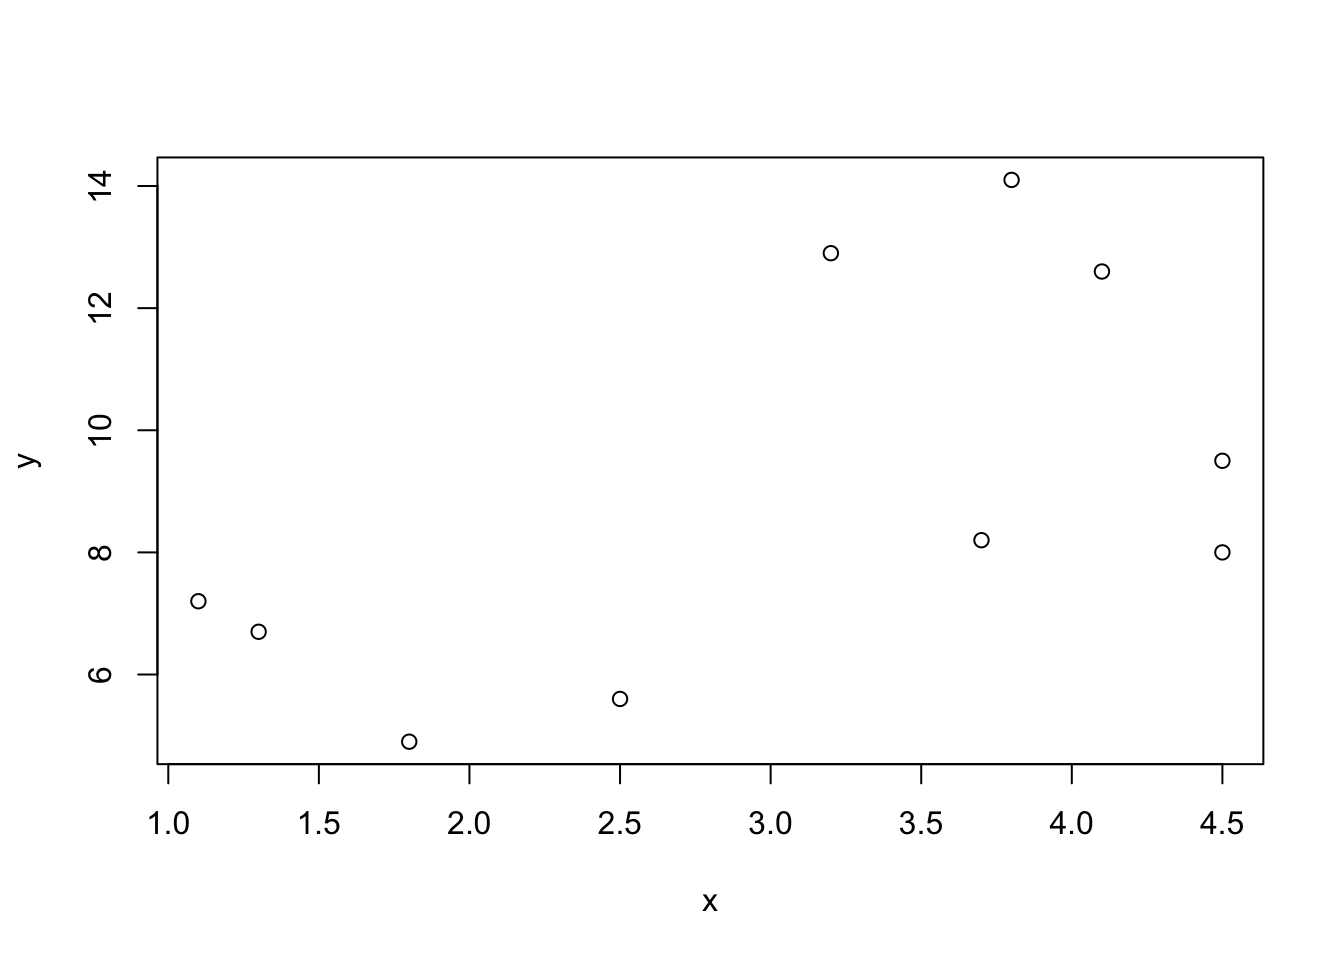
\includegraphics[width=0.6\linewidth]{statthink_files/figure-latex/Regression1-1} 

}

\caption{A Scatter Plot}\label{fig:Regression1}
\end{figure}

The scatter plot that is produced by the last expression is presented in
Figure~\ref{fig:Regression1}.

A scatter plot is a graph that displays jointly the data of two
numerical variables. The variables (``\texttt{x}'' and ``\texttt{y}'' in this case) are
represented by the \(x\)-axis and the \(y\)-axis, respectively. The \(x\)-axis
is associated with the explanatory variable and the \(y\)-axis is
associated with the response.

Each observation is represented by a point. The \(x\)-value of the point
corresponds to the value of the explanatory variable for the observation
and the \(y\)-value corresponds to the value of the response. For example,
the first observation is represented by the point \((x=4.5,y=9.5)\). The
two rightmost points have an \(x\) value of 4.5. The higher of the two has
a \(y\) value of 9.5 and is therefore point associated with the first
observation. The lower of the two has a \(y\) value of 8.0, and is thus
associated with the 8th observation. Altogether there are 10 points in
the plot, corresponding to the 10 observations in the data frame.

Let us consider another example of a scatter plot. The file ``\texttt{cars.csv}''
contains data regarding characteristics of cars. Among the variables in
this data frame are the variables ``\texttt{horsepower}'' and the variable
``\texttt{engine.size}''. Both variables are numeric.

The variable ``\texttt{engine.size}'' describes the volume, in cubic inches, that
is swept by all the pistons inside the cylinders. The variable
``\texttt{horsepower}'' measures the power of the engine in units of horsepower.
Let us examine the relation between these two variables with a scatter
plot:

\begin{Shaded}
\begin{Highlighting}[]
\NormalTok{cars <-}\StringTok{ }\KeywordTok{read.csv}\NormalTok{(}\StringTok{"_data/cars.csv"}\NormalTok{)}
\KeywordTok{plot}\NormalTok{(horsepower }\OperatorTok{~}\StringTok{ }\NormalTok{engine.size, }\DataTypeTok{data=}\NormalTok{cars)}
\end{Highlighting}
\end{Shaded}

\begin{figure}

{\centering 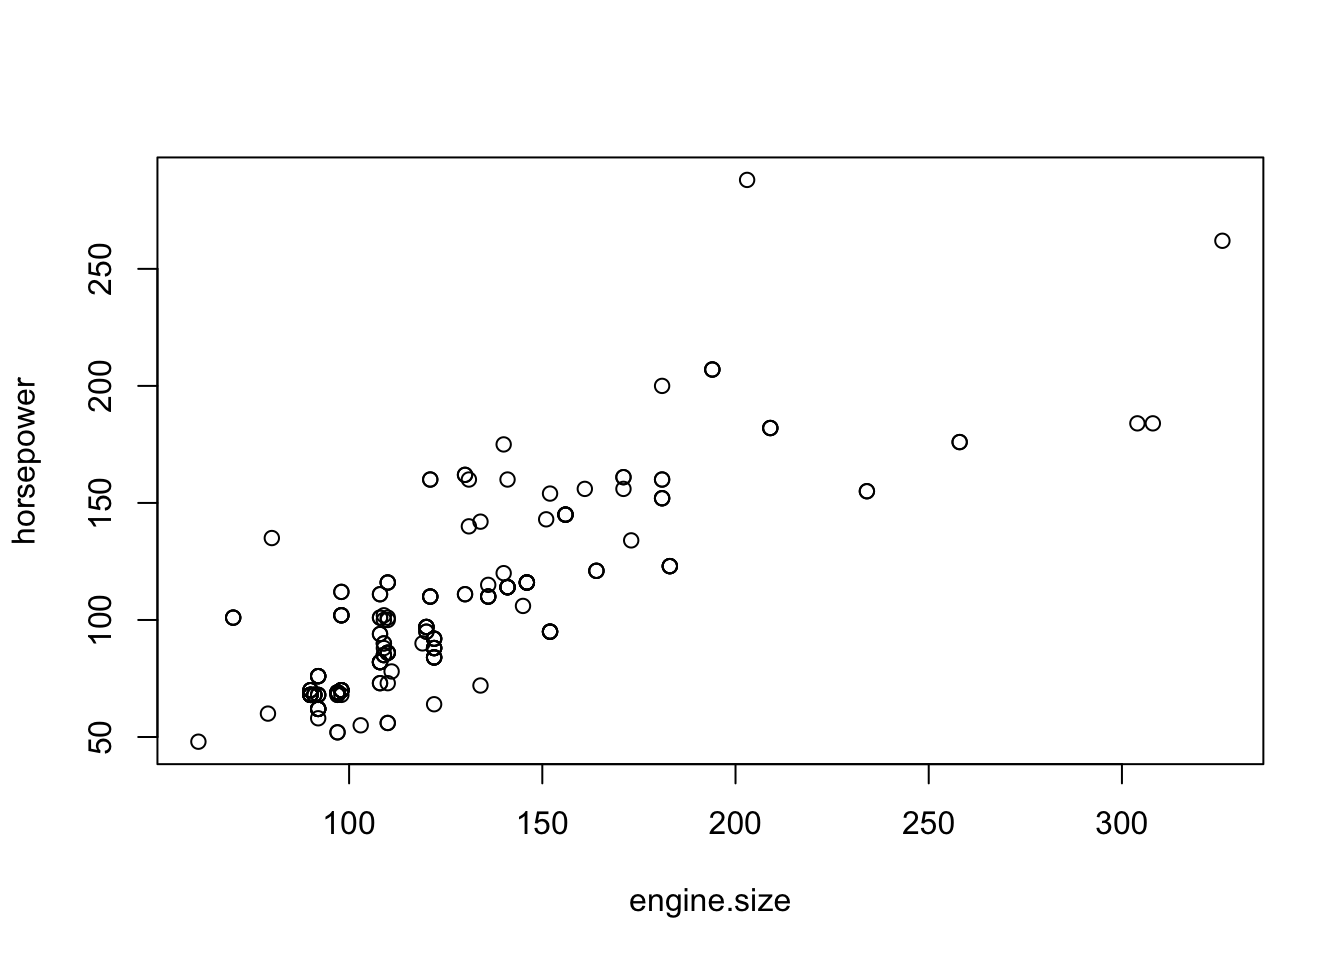
\includegraphics[width=0.6\linewidth]{statthink_files/figure-latex/Regression2-1} 

}

\caption{The Scatter Plot of Power versus Engine Size}\label{fig:Regression2}
\end{figure}

In the first line of code we read the data from the file into an \texttt{R}
data frame that is given the name ``\texttt{cars}''. In the second line we
produce the scatter plot with ``\texttt{horsepower}'' as the response and
``\texttt{engine.size}'' as the explanatory variable. Both variables are taken
from the data frame ``\texttt{cars}''. The plot that is produced by the last
expression is presented in Figure~\[fig:Regression\_2\].

Consider the expression ``\texttt{plot(horsepower\textasciitilde{}engine.size,\ data=cars)}''.
Both the response variable and the explanatory variables that are given
in this expression do not exist in the computer's memory as independent
objects, but only as variables within the object ``\texttt{cars}''. In some
cases, however, one may refer to these variables directly within the
function, provided that the argument ``\texttt{data=}\emph{data.frame.name}'' is added
to the function. This argument informs the function in which data frame
the variables can be found, where \emph{data.frame.name} is the name of the
data frame. In the current example, the variables are located in the
data frame ``\texttt{cars}''.

Examine the scatter plot in Figure~\ref{fig:Regression2}. One may see
that the values of the response (\texttt{horsepower}) tend to increase with the
increase in the values of the explanatory variable (\texttt{engine.size}).
Overall, the increase tends to follow a linear trend, a straight line,
although the data points are not located exactly on a single line. The
role of linear regression, which will be discussed in the subsequent
sections, is to describe and assess this linear trend.

\hypertarget{linear-equation}{%
\subsection{Linear Equation}\label{linear-equation}}

Linear regression describes linear trends in the relation between a
response and an explanatory variable. Linear trends may be specified
with the aid of linear equations. In this subsection we discuss the
relation between a linear equation and a linear trend (a straight line).

A linear equation is an equation of the form:

\[y = a + b \cdot x\;,\]
where \(y\) and \(x\) are variables and \(a\) and \(b\) are the coefficients of
the equation. The coefficient \(a\) is called the \emph{intercept} and the
coefficient \(b\) is called the \emph{slope}.

A linear equation can be used in order to plot a line on a graph. With
each value on the \(x\)-axis one may associate a value on the \(y\)-axis:
the value that satisfies the linear equation. The collection of all such
pairs of points, all possible \(x\) values and their associated \(y\)
values, produces a straight line in the two-dimensional plane.

\begin{figure}

{\centering 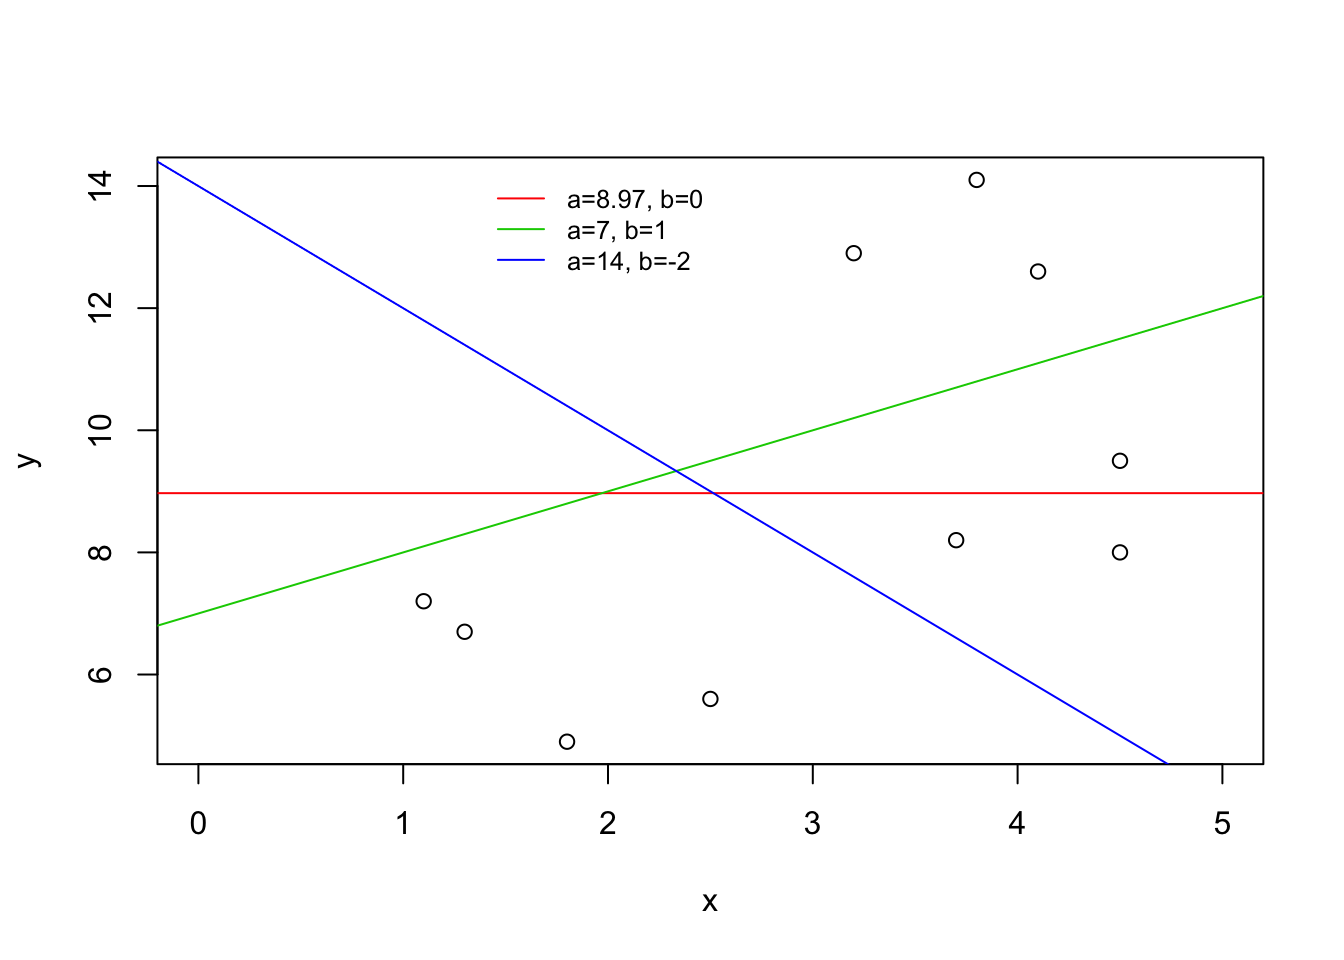
\includegraphics[width=0.6\linewidth]{statthink_files/figure-latex/Regression3-1} 

}

\caption{Lines}\label{fig:Regression3}
\end{figure}

As an illustration consider the three lines in
Figure~\ref{fig:Regression3}. The \emph{green} line is produced via the
equation \(y = 7 + x\), the intercept of the line is 7 and the slope is 1.
The \emph{blue} is a result of the equation \(y = 14 - 2 x\). For this line the
intercept is 14 and the slope is -2. Finally, the \emph{red} line is produced
by the equation \(y = 8.97\). The intercept of the line is 8.97 and the
slope is equal to 0.

The intercept describes the value of \(y\) when the line crosses the
\(y\)-axis. Equivalently, it is the result of the application of the
linear equation for the value \(x=0\). Observe in
Figure~\ref{fig:Regression3} that the \emph{green} line crosses the \(y\)-axis
at the level \(y=7\). Likewise, the \emph{blue} line crosses the \(y\)-axis at
the level \(y=14\). The \emph{red} line stays constantly at the level \(y=8.97\),
and this is also the level at which it crosses the \(y\)-axis.

The slope is the change in the value of \(y\) for each unit change in the
value of \(x\). Consider the \emph{green} line. When \(x=0\) the value of \(y\) is
\(y=7\). When \(x\) changes to \(x=1\) then the value of \(y\) changes to \(y=8\).
A change of one unit in \(x\) corresponds to an \emph{increase} in one unit in
\(y\). Indeed, the slope for this line is \(b=1\). As for the \emph{blue} line,
when \(x\) changes from 0 to 1 the value of \(y\) changes from \(y=14\) to
\(y=12\); a \emph{decrease} of two units. This decrease is associated with the
slope \(b=-2\). Lastly, for the constant \emph{red} line there is no change in
the value of \(y\) when \(x\) changes its value from \(x=0\) to \(x=1\).
Therefore, the slope is \(b=0\). A positive slope is associated with an
increasing line, a negative slope is associated with a decreasing line
and a zero slope is associated with a constant line.

Lines can be considered in the context of scatter plots.
Figure~\ref{fig:Regression3} contains the scatter plot of the data on
the relation between the length of fish and their weight. A regression
line is the line that best describes the linear trend of the relation
between the explanatory variable and the response. Neither of the lines
in the figure is the regression line, although the \emph{green} line is a
better description of the trend than the \emph{blue} line. The regression
line is the best description of the linear trend.

The \emph{red} line is a fixed line that is constructed at a level equal to
the average value\footnote{Run the expression ``\texttt{mean(y)}'' to obtain \(\bar y = 8.97\) as the
  value of the sample average.} of the variable \(y\). This line partly reflects the
information in the data. The regression line, which we fit in the next
section, reflects more of the information by including a description of
the trend in the data.

Lastly, let us see how one can add lines to a plot in \texttt{R}. Functions to
produce plots in \texttt{R} can be divided into two categories: high level and
low level plotting functions. High level functions produce an entire
plot, including the axes and the labels of the plot. The plotting
functions that we encountered in the past such as ``\texttt{plot}'', ``\texttt{hist}'',
``\texttt{boxplot}'' and the like are all high level plotting functions. Low
level functions, on the other hand, add features to an existing plot.

An example of a low level plotting function is the function ``\texttt{abline}''.
This function adds a straight line to an existing plot. The first
argument to the function is the intercept of the line and the second
argument is the slope of the line. Other arguments may be used in order
to specify the characteristics of the line. For example, the argument
``\texttt{col=}\emph{color.name}'' may be used in order to change the color of the
line from its default black color. A plot that is very similar to plot
in Figure~\ref{fig:Regression3} may be produced with the following
code\footnote{The actual plot in Figure~\[fig:Regression\_3\] is produced by a
  slightly modified code. First an empty plot is produced with the
  expression ``\texttt{plot(c(0,5),c(5,15),type=n,xlab=x,ylab=y)}'' and then
  the points are added with the expression ``\texttt{points(y\textasciitilde{}x)}''. The lines
  are added as in the text. Finally, a legend is added with the
  function ``\texttt{legend}''.}:

\begin{Shaded}
\begin{Highlighting}[]
\KeywordTok{plot}\NormalTok{(y}\OperatorTok{~}\NormalTok{x)}
\KeywordTok{abline}\NormalTok{(}\DecValTok{7}\NormalTok{,}\DecValTok{1}\NormalTok{,}\DataTypeTok{col=}\StringTok{"green"}\NormalTok{)}
\KeywordTok{abline}\NormalTok{(}\DecValTok{14}\NormalTok{,}\OperatorTok{-}\DecValTok{2}\NormalTok{,}\DataTypeTok{col=}\StringTok{"blue"}\NormalTok{)}
\KeywordTok{abline}\NormalTok{(}\KeywordTok{mean}\NormalTok{(y),}\DecValTok{0}\NormalTok{,}\DataTypeTok{col=}\StringTok{"red"}\NormalTok{)}
\end{Highlighting}
\end{Shaded}

\begin{center}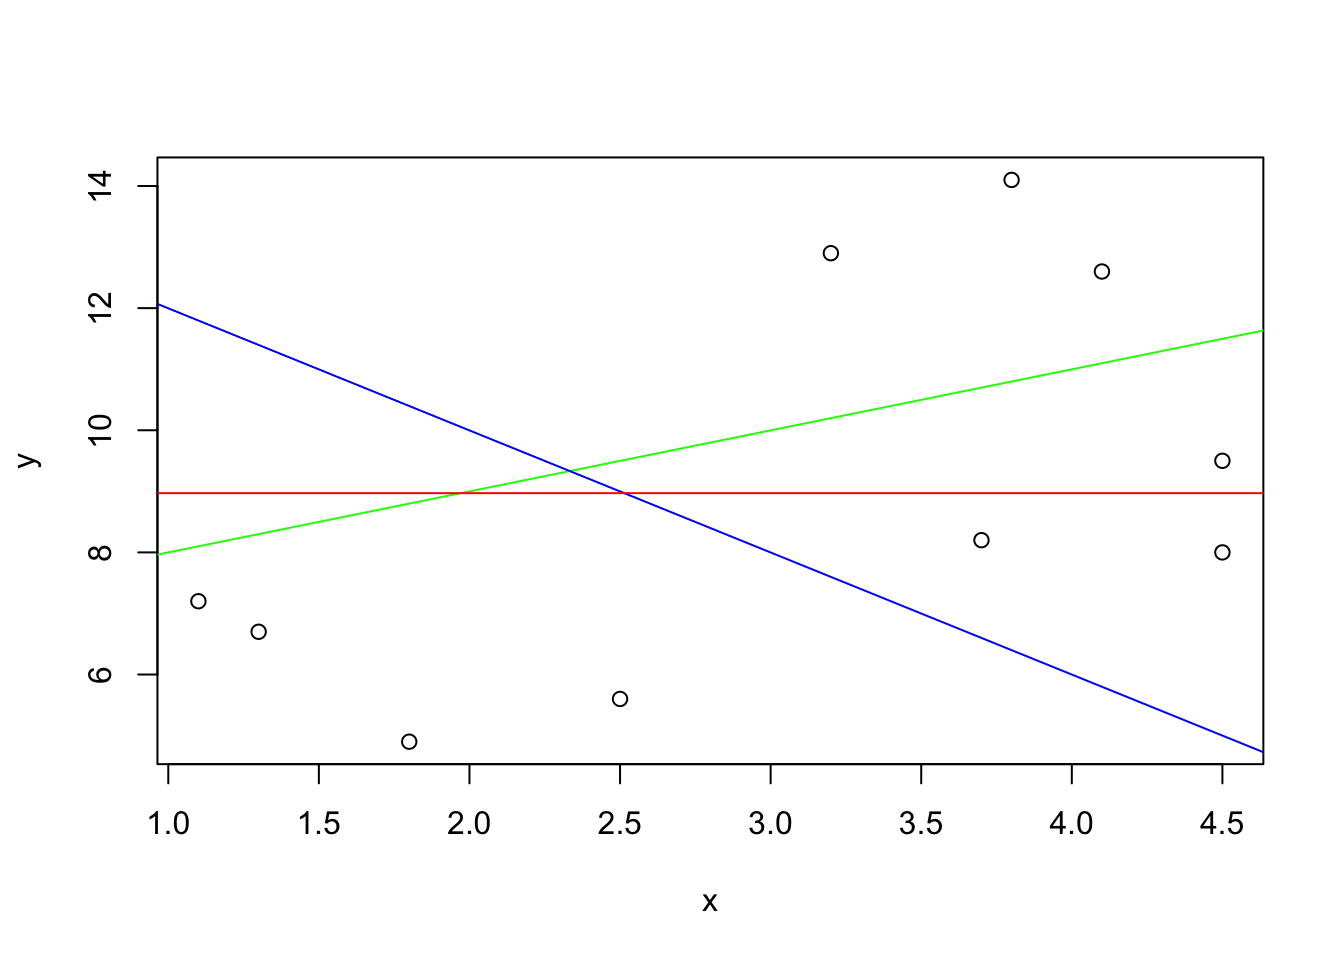
\includegraphics[width=0.6\linewidth]{statthink_files/figure-latex/unnamed-chunk-205-1} \end{center}

Initially, the scatter plot is created and the lines are added to the
plot one after the other. Observe that color of the first line that is
added is green, it has an intercept of 7 and a slope of 1. The second
line is blue, with a intercept of 14 and a negative slope of -2. The
last line is red, and its constant value is the average of the variable
\(y\).

In the next section we discuss the computation of the regression line,
the line that describes the linear trend in the data. This line will be
added to scatter plots with the aid of the function ``\texttt{abline}''.

\hypertarget{linear-regression}{%
\section{Linear Regression}\label{linear-regression}}

Data that describes the joint distribution of two numeric variables can
be represented with a scatter plot. The \(y\)-axis in this plot
corresponds to the response and the \(x\)-axis corresponds to the
explanatory variable. The regression line describes the linear trend of
the response as a function of the explanatory variable. This line is
characterized by a linear equation with an intercept and a slope that
are computed from the data.

In the first subsection we present the computation of the regression
linear equation from the data. The second subsection discusses
regression as a statistical model. Statistical inference can be carried
out on the basis of this model. In the context of the statistical model,
one may consider the intercept and the slope of the regression model
that is fitted to the data as point estimates of the model's parameter.
Based on these estimates, one may test hypotheses regarding the
regression model and construct confidence intervals for parameters.

\hypertarget{fitting-the-regression-line}{%
\subsection{Fitting the Regression Line}\label{fitting-the-regression-line}}

The \texttt{R} function that fits the regression line to data is called ``\texttt{lm}'',
an acronym for \emph{Linear Model}. The input to the function is a formula,
with the response variable to the left of the tilde character and the
explanatory variable to the right of it. The output of the function is
the fitted linear regression model.

Let us apply the linear regression function to the data on the weight
and the length of fish. The output of the function is saved by us in a
object called ``\texttt{fit}''. Subsequently, the content of the object ``\texttt{fit}''
is displayed:

\begin{Shaded}
\begin{Highlighting}[]
\NormalTok{fit <-}\StringTok{ }\KeywordTok{lm}\NormalTok{(y}\OperatorTok{~}\NormalTok{x)}
\NormalTok{fit}
\end{Highlighting}
\end{Shaded}

\begin{verbatim}
## 
## Call:
## lm(formula = y ~ x)
## 
## Coefficients:
## (Intercept)            x  
##      4.6165       1.4274
\end{verbatim}

When displayed, the output of the function ``\texttt{lm}'' shows the formula that
was used by the function and provides the coefficients of the regression
linear equation. Observe that the intercept of the line is equal to
4.616. The slope of the line, the coefficient that multiplies ``\texttt{x}'' in
linear equation, is equal to 1.427.

One may add the regression line to the scatter plot with the aid of the
function ``\texttt{abline}'':

\begin{Shaded}
\begin{Highlighting}[]
\KeywordTok{plot}\NormalTok{(y}\OperatorTok{~}\NormalTok{x)}
\KeywordTok{abline}\NormalTok{(fit)}
\end{Highlighting}
\end{Shaded}

\begin{figure}

{\centering 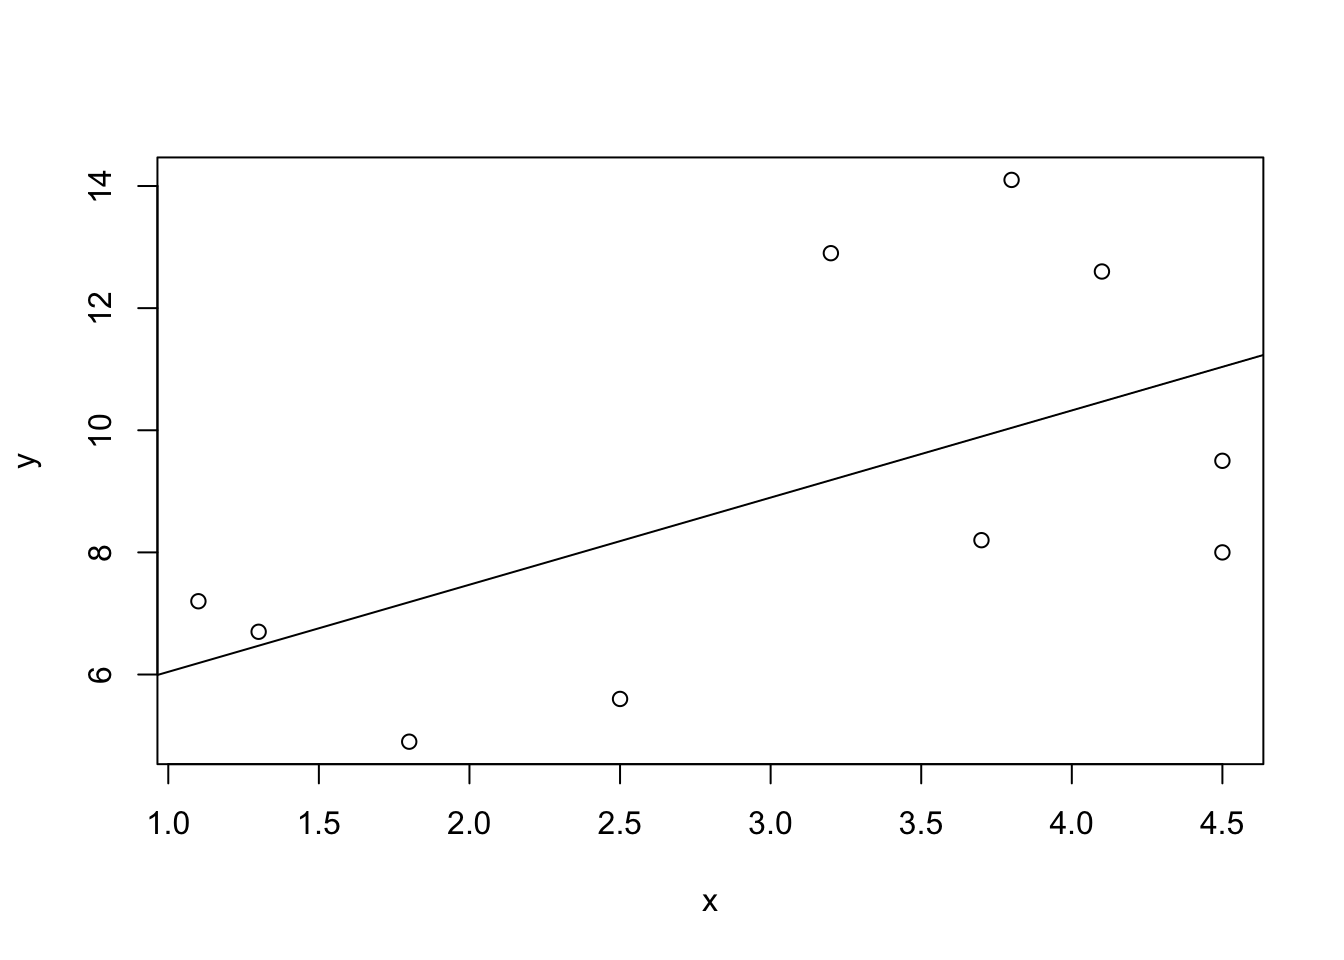
\includegraphics[width=0.6\linewidth]{statthink_files/figure-latex/Regression4-1} 

}

\caption{A Fitted Regression Line}\label{fig:Regression4}
\end{figure}

The first expression produces the scatter plot of the data on fish. The
second expression adds the regression line to the scatter plot. When the
input to the graphical function ``\texttt{abline}'' is the output of the function
``\texttt{lm}'' that fits the regression line, then the result is the addition of
the regression line to the existing plot. The line that is added is the
line characterized by the coefficients that are computed by the function
``\texttt{lm}''. The coefficients in the current setting are 4.616 for the
intercept and 1.427 for the slope.

The scatter plot and the added regression line are displayed in
Figure~\ref{fig:Regression4}. Observe that line passes through the
points, balancing between the points that are above the line and the
points that are below. The line captures the linear trend in the data.

Examine the line in Figure~\ref{fig:Regression4}. When \(x=1\) then the
\(y\) value of the line is slightly above 6. When the value of \(x\) is
equal to 2, a change of one unit, then value of \(y\) is below 8, and is
approximately equal to 7.5. This observation is consistent with the fact
that the slop of the line is 1.427. The value of \(x\) is decreased by 1
when changing from \(x=1\) to \(x=0\). Consequently, the value of \(y\) when
\(x=0\) should decrease by 1.427 in comparison to its value when \(x=1\).
The value at \(x=1\) is approximately 6. Therefore, the value at \(x=0\)
should be approximately 4.6. Indeed, we do get that the intercept is
equal to 4.616.

The coefficients of the regression line are computed from the data and
are hence statistics. Specifically, the slope of the regression line is
computed as the ratio between the \emph{covariance} of the response and the
explanatory variable, divided by the variance of the explanatory
variable. The intercept of the regression line is computed using the
sample averages of both variables and the computed slope.

Start with the slope. The main ingredient in the formula for the slope,
the numerator in the ratio, is the covariance between the two variables.
The covariance measures the joint variability of two variables. Recall
that the formula for the sample variance of the variable \(x\) is equal
to::

\[s^2 = \frac{\mbox{Sum of the squares of the deviations}}{\mbox{Number of values in the sample}-1} = \frac{\sum_{i=1}^n (x_i - \bar x)^2}{n-1}\;.\]
The formula of the sample covariance between \(x\) and \(y\) replaces the
square of the deviations by the product of deviations. The product is
between an \(y\) deviation and the parallel \(x\) deviation:

\[\mbox{covariance} = \frac{\mbox{Sum of products of the deviations}}{\mbox{Number of values in the sample}-1} = \frac{\sum_{i=1}^n (y_i-\bar y)(x_i - \bar x)}{n-1}\;.\]

The function ``\texttt{cov}'' computes the sample covariance between two numeric
variables. The two variables enter as arguments to the function and the
sample covariance is the output. Let us demonstrate the computation by
first applying the given function to the data on fish and then repeating
the computations without the aid of the function:

\begin{Shaded}
\begin{Highlighting}[]
\KeywordTok{cov}\NormalTok{(y,x)}
\end{Highlighting}
\end{Shaded}

\begin{verbatim}
## [1] 2.3861111
\end{verbatim}

\begin{Shaded}
\begin{Highlighting}[]
\KeywordTok{sum}\NormalTok{((y}\OperatorTok{-}\KeywordTok{mean}\NormalTok{(y))}\OperatorTok{*}\NormalTok{(x}\OperatorTok{-}\KeywordTok{mean}\NormalTok{(x)))}\OperatorTok{/}\DecValTok{9}
\end{Highlighting}
\end{Shaded}

\begin{verbatim}
## [1] 2.3861111
\end{verbatim}

In both cases we obtained the same result. Notice that the sum of
products of deviations in the second expression was divided by 9, which
is the number of observations, minus 1.

The slope of the regression line is the ratio between the covariance and
the variance of the explanatory variable.

The regression line passes through the point \((\bar x, \bar y)\), a point
that is determined by the means of the both the explanatory variable and
the response. It follows that the intercept should obey the equation:

\[\bar y = a + b\cdot \bar x \quad\Longrightarrow\quad a = \bar y - b\cdot \bar x\;,\]
The left-hand-side equation corresponds to the statement that the value
of the regression line at the average \(\bar x\) is equal to the average
of the response \(\bar y\). The right-hand-side equation is the solution
to the left-hand-side equation.

One may compute the coefficients of the regression model manually by
computing first the slope as a ratio between the covariance and the
variance of explanatory variable. The intercept can then be obtained by
the equation that uses the computed slope and the averages of both
variables:

\begin{Shaded}
\begin{Highlighting}[]
\NormalTok{b <-}\StringTok{ }\KeywordTok{cov}\NormalTok{(x,y)}\OperatorTok{/}\KeywordTok{var}\NormalTok{(x)}
\NormalTok{a <-}\StringTok{ }\KeywordTok{mean}\NormalTok{(y) }\OperatorTok{-}\StringTok{ }\NormalTok{b}\OperatorTok{*}\KeywordTok{mean}\NormalTok{(x)}
\NormalTok{a}
\end{Highlighting}
\end{Shaded}

\begin{verbatim}
## [1] 4.6164772
\end{verbatim}

\begin{Shaded}
\begin{Highlighting}[]
\NormalTok{b}
\end{Highlighting}
\end{Shaded}

\begin{verbatim}
## [1] 1.4273845
\end{verbatim}

Applying the manual method we obtain, after rounding up, the same
coefficients that were produced by the application of the function
``\texttt{lm}'' to the data.

As an exercise, let us fit the regression model to the data on the
relation between the response ``\texttt{horsepower}'' and the explanatory
variable ``\texttt{engine.size}''. Apply the function ``\texttt{lm}'' to the data and
present the results:

\begin{Shaded}
\begin{Highlighting}[]
\NormalTok{fit.power <-}\StringTok{ }\KeywordTok{lm}\NormalTok{(horsepower }\OperatorTok{~}\StringTok{ }\NormalTok{engine.size, }\DataTypeTok{data=}\NormalTok{cars)}
\NormalTok{fit.power}
\end{Highlighting}
\end{Shaded}

\begin{verbatim}
## 
## Call:
## lm(formula = horsepower ~ engine.size, data = cars)
## 
## Coefficients:
## (Intercept)  engine.size  
##     6.64138      0.76949
\end{verbatim}

The fitted regression model is stored in an object called ``\texttt{fit.power}''.
The intercept in the current setting is equal to 6.6414 and the slope is
equal to 0.7695.

Observe that one may refer to variables that belong to a data frame,
provided that the name of the data frame is entered as the value of the
argument ``\texttt{data}'' in the function ``\texttt{lm}''. Here we refer to variables
that belong to the data frame ``\texttt{cars}''.

Next we plot the scatter plot of the data and add the regression line:

\begin{Shaded}
\begin{Highlighting}[]
\KeywordTok{plot}\NormalTok{(horsepower }\OperatorTok{~}\StringTok{ }\NormalTok{engine.size, }\DataTypeTok{data=}\NormalTok{cars)}
\KeywordTok{abline}\NormalTok{(fit.power)}
\end{Highlighting}
\end{Shaded}

\begin{figure}

{\centering 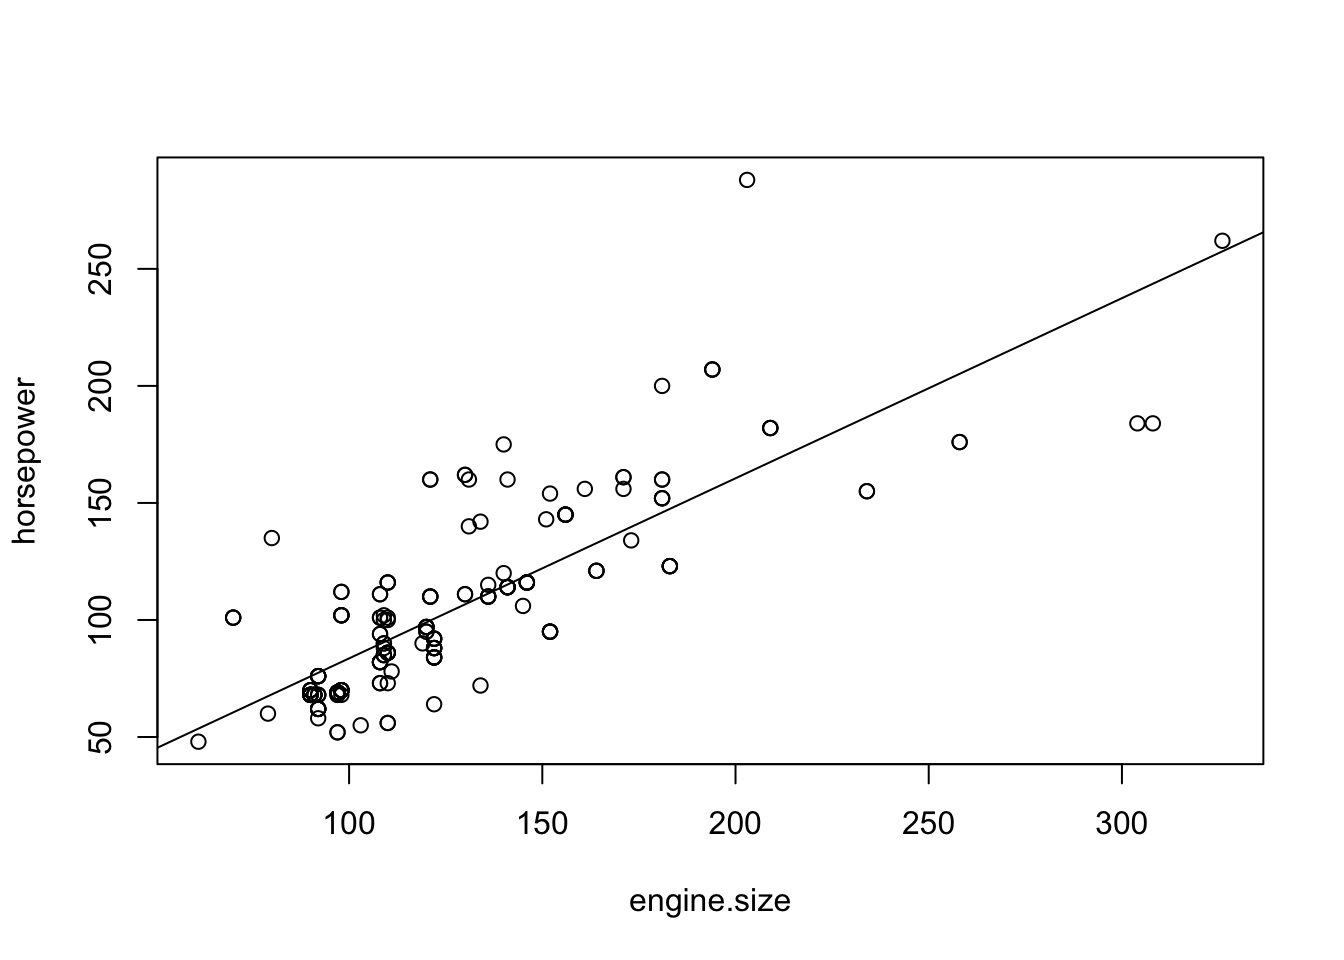
\includegraphics[width=0.6\linewidth]{statthink_files/figure-latex/Regression5-1} 

}

\caption{A Regression Model of Power versus Engine Size}\label{fig:Regression5}
\end{figure}

The output of the plotting functions is presented in
Figure~\ref{fig:Regression5}. Again, the regression line describes the
general linear trend in the data. Overall, with the increase in engine
size one observes increase in the power of the engine.

\hypertarget{subsec:Inference}{%
\subsection{Inference}\label{subsec:Inference}}

Up to this point we have been considering the regression model in the
context of descriptive statistics. The aim in fitting the regression
line to the data was to characterize the linear trend observed in the
data. Our next goal is to deal with regression in the context of
inferential statistics. The goal here is to produce statements on
characteristics of an entire population on the basis of the data
contained in the sample.

The foundation for statistical inference in a given setting is a
statistical model that produces the sampling distribution in that
setting. The sampling distribution is the frame of reference for the
analysis. In this context, the observed sample is a single realization
of the sampling distribution, one realization among infinitely many
potential realizations that never take place. The setting of regression
involves a response and an explanatory variable. We provide a
description of the statistical model for this setting.

The relation between the response and the explanatory variable is such
that the value of the later affects the distribution of the former.
Still, the value of the response is not uniquely defined by the value of
the explanatory variable. This principle also hold for the regression
model of the relation between the response \(Y\) and the explanatory
variable \(X\). According to the model of linear regression the value of
the \emph{expectation} of the response for observation \(i\), \(\Expec(Y_i)\), is
a linear function of the value of the explanatory variable for the same
observation. Hence, there exist and intercept \(a\) and a slope \(b\),
common for all observations, such that if \(X_i = x_i\) then

\[\Expec(Y_i) = a + b \cdot x_i\;.\] The regression line can thus be
interpreted as the average trend of the response in the population. This
average trend is a linear function of the explanatory variable.

The intercept \(a\) and the slope \(b\) of the statistical model are
parameters of the sampling distribution. One may test hypotheses and
construct confidence intervals for these parameters based on the
observed data and in relation to the sampling distribution.

Consider testing hypothesis. A natural null hypothesis to consider is
the hypothesis that the slope is equal to zero. This hypothesis
corresponds to statement that the expected value of the response is
constant for all values of the explanatory variable. In other words, the
hypothesis is that the explanatory variable does not affect the
distribution of the response\footnote{According to the model of linear regression, the only effect of
  the explanatory variable on the distribution of the response is via
  the expectation. If such an effect, according to the null
  hypothesis, is also excluded then the so called explanatory variable
  is not effecting at all the distribution of the response.}. One may formulate this null hypothesis
as \(H_0:b = 0\) and test it against the alternative \(H_1: b \not= 0\) that
states that the explanatory variable does affect the distribution of the
response.

A test of the given hypotheses can be carried out by the application of
the function ``\texttt{summary}'' to the output of the function ``\texttt{lm}''. Recall
that the function ``\texttt{lm}'' was used in order to fit the linear regression
to the data. In particular, this function was applied to the data on the
relation between the size of the engine and the power that the engine
produces. The function fitted a regression line that describes the
linear trend of the data. The output of the function was saved in an
object by the name ``\texttt{fit.power}''. We apply the function ``\texttt{summary}'' to
this object:

\begin{Shaded}
\begin{Highlighting}[]
\KeywordTok{summary}\NormalTok{(fit.power)}
\end{Highlighting}
\end{Shaded}

\begin{verbatim}
## 
## Call:
## lm(formula = horsepower ~ engine.size, data = cars)
## 
## Residuals:
##      Min       1Q   Median       3Q      Max 
## -59.6430 -12.2815  -5.5153  10.2508 125.1530 
## 
## Coefficients:
##             Estimate Std. Error t value Pr(>|t|)    
## (Intercept) 6.641379   5.233181  1.2691   0.2059    
## engine.size 0.769486   0.039186 19.6369   <2e-16 ***
## ---
## Signif. codes:  0 '***' 0.001 '**' 0.01 '*' 0.05 '.' 0.1 ' ' 1
## 
## Residual standard error: 23.305 on 201 degrees of freedom
##   (2 observations deleted due to missingness)
## Multiple R-squared:  0.65735,    Adjusted R-squared:  0.65565 
## F-statistic: 385.61 on 1 and 201 DF,  p-value: < 2.22e-16
\end{verbatim}

The output produced by the application of the function ``\texttt{summary}'' is
long and detailed. We will discuss this output in the next section. Here
we concentrate on the table that goes under the title ``\texttt{Coefficients:}''.
The said table is made of 2 rows and 4 columns. It contains information
for testing, for each of the coefficients, the null hypothesis that the
value of the given coefficient is equal to zero. In particular, the
second row may be used is order to test this hypothesis for the slope of
the regression line, the coefficient that multiplies the explanatory
variable.

Consider the second row. The first value on this row is 0.76949, which
is equal (after rounding up) to the slope of the line that was fitted to
the data in the previous subsection. However, in the context of
statistical inference this value is the \emph{estimate} of the slope of the
population regression coefficient, the realization of the estimator of
the slope\footnote{The estimator of the slope is obtained via the application of the
  formula for the computation of the slope to the sample:
  \(\frac{1}{n-1}\sum_{i=1}^n (Y_i-\bar Y)(X_i - \bar X)/\frac{1}{n-1}\sum_{i=1}^n (X_i - \bar X)^2\).}.

The second value is 0.03919. This is an estimate of the standard
deviation of the estimator of the slope. The third value is the test
statistic. This statistic is the ratio between the deviation of the
sample estimate of the parameter (0.76949) from the value of the
parameter under the null hypothesis (0), divided by the estimated
standard deviation (0.03919):
\((0.76949 - 0)/0.03919 = 0.76949/0.03919 = 19.63486\), which is
essentially the value given in the report\footnote{Our computation involves rounding up errors, hence the small
  discrepancy between the value we computed and the value in the
  report.}.

The last value is the computed \(p\)-value for the test. It can be shown
that the sampling distribution of the given test statistic, under the
null distribution which assumes no slope, is asymptotically the standard
Normal distribution. If the distribution of the response itself is
Normal then the distribution of the statistic is the \(t\)-distribution on
\(n-2\) degrees of freedom. In the current situation this corresponds to
201 degrees of freedom\footnote{Notice that the ``\texttt{horsepower}'' measurement is missing for two
  observation. These observations are deleted for the analysis,
  leaving a total of \(n=203\) observations. The number of degrees of
  freedom is \(n-2 = 203-2=201\).}. The computed \(p\)-value is extremely small,
practically eliminating the possibility that the slope is equal to zero.

The first row presents information regarding the intercept. The
estimated intercept is 6.64138 with an estimated standard deviation of
5.23318. The value of the test statistic is 1.269 and the \(p\)-value for
testing the null hypothesis that the intercept is equal to zero against
the two sided alternative is 0.206. In this case the null hypothesis is
not rejected since the \(p\)-value is larger than 0.05.

The report contains an inference for the intercept. However, one is
advised to take this inference in the current case with a grain of salt.
Indeed, the intercept is the expected value of the response when the
explanatory variable is equal to zero. Here the explanatory variable is
the size of the engine and the response is the power of that engine. The
power of an engine of size zero is a quantity that has no physical
meaning! In general, unless the intercept is in the range of
observations (i.e.~the value 0 is in the range of the observed
explanatory variable) one should treat the inference on the intercept
cautiously. Such inference requires extrapolation and is sensitive to
the miss-specification of the regression model.

Apart from testing hypotheses one may also construct confidence
intervals for the parameters. A crude confidence interval may be
obtained by taking 1.96 standard deviations on each side of the estimate
of the parameter. Hence, a confidence interval for the slope is
approximately equal to
\(0.76949 \pm 1.96\times 0.03919 = [0.6926776, 0.8463024]\). In a similar
way one may obtain a confidence interval for the slope\footnote{The warning message that was made in the context of testing
  hypotheses on the intercept should be applied also to the
  construction of confidence intervals. If the value 0 is not in the
  range of the explanatory variable then one should be careful when
  interpreting a confidence interval for the intercept.}:
\(6.64138 \pm 1.96\times 5.23318 = [-3.615653, 16.89841]\).

Alternatively, one may compute confidence intervals for the parameters
of the linear regression model using the function ``\texttt{confint}''. The input
to this function is the fitted model and the output is a confidence
interval for each of the parameters:

\begin{Shaded}
\begin{Highlighting}[]
\KeywordTok{confint}\NormalTok{(fit.power)}
\end{Highlighting}
\end{Shaded}

\begin{verbatim}
##                   2.5 %      97.5 %
## (Intercept) -3.67759894 16.96035643
## engine.size  0.69221808  0.84675366
\end{verbatim}

Observe the similarity between the confidence intervals that are
computed by the function and the crude confidence intervals that were
produced by us. The small discrepancies that do exist between the
intervals result from the fact that the function ``\texttt{confint}'' uses the
\(t\)-distribution whereas we used the Normal approximation.

\hypertarget{r-squared-and-the-variance-of-residuals}{%
\section{R-squared and the Variance of Residuals}\label{r-squared-and-the-variance-of-residuals}}

In this section we discuss the residuals between the values of the
response and their estimated expected value according to the regression
model. These residuals are the regression model equivalence of the
deviations between the observations and the sample average. We use these
residuals in order compute the variability that is not accounted for by
the regression model. Indeed, the ratio between the total variability of
the residuals and the total variability of the deviations from the
average serves as a measure of the variability that is not explained by
the explanatory variable. R-squared, which is equal to 1 minus this
ratio, is interpreted as the fraction of the variability of the response
that is explained by the regression model.

We start with the definition of residuals. Let us return to the
artificial example that compared length of fish to their weight. The
data for this example was given in Table~\[tab:Regression\_1\] and was
saved in the objects ``\texttt{x}'' and ``\texttt{y}''. The regression model was fitted to
this data by the application of the function ``\texttt{lm}'' to the formula
``\texttt{y\textasciitilde{}x}'' and the fitted model was saved in an object called ``\texttt{fit}''. Let
us apply the function ``\texttt{summary}'' to the fitted model:

\begin{Shaded}
\begin{Highlighting}[]
\KeywordTok{summary}\NormalTok{(fit)}
\end{Highlighting}
\end{Shaded}

\begin{verbatim}
## 
## Call:
## lm(formula = y ~ x)
## 
## Residuals:
##      Min       1Q   Median       3Q      Max 
## -3.03971 -2.13878 -0.65589  1.85178  4.05946 
## 
## Coefficients:
##             Estimate Std. Error t value Pr(>|t|)  
## (Intercept)   4.6165     2.3653  1.9518  0.08676 .
## x             1.4274     0.7195  1.9839  0.08255 .
## ---
## Signif. codes:  0 '***' 0.001 '**' 0.01 '*' 0.05 '.' 0.1 ' ' 1
## 
## Residual standard error: 2.7908 on 8 degrees of freedom
## Multiple R-squared:  0.32974,    Adjusted R-squared:  0.24596 
## F-statistic: 3.9357 on 1 and 8 DF,  p-value: 0.082554
\end{verbatim}

The given report contains a table with estimates of the regression
coefficients and information for conducting hypothesis testing. The
report contains other information that is associated mainly with the
notion of the residuals from regression line. Our current goal is to
understand what is that other information.

The residual from regression for each observation is the difference
between the value of the response for the observation and the estimated
expectation of the response under the regression model\footnote{The estimated expectation of the response is also called \emph{the
  predicted response}.}. An
observation is a pair \((x_i,y_i)\), with \(y_i\) being the value of the
response. The expectation of the response according to the regression
model is \(a + b \cdot x_i\), where \(a\) and \(b\) are the coefficients of
the model. The estimated expectation is obtained by using, in the
formula for the expectation, the coefficients that are estimated from
the data. The residual is the difference between \(y_i\) and
\(a + b \cdot x_i\).

Consider an example. The first observation on the fish is \((4.5, 9.5)\),
where \(x_1 = 4.5\) and \(y_1 = 9.5\). The estimated intercept is 4.6165 and
the estimated slope is 1.4274. The estimated expectation of the response
for the first variable is equal to

\[4.6165 + 1.4274 \cdot x_1 = 4.6165 + 1.4274 \cdot 4.5  =  11.0398\;.\]
The residual is the difference between the observes response and this
value:

\[y_1 - (4.6165 + 1.4274 \cdot x_1) = 9.5 - 11.0398 = -1.5398\;.\]

The residuals for the other observations are computed in the same
manner. The values of the intercept and the slope are kept the same but
the values of the explanatory variable and the response are changed.

\begin{figure}

{\centering 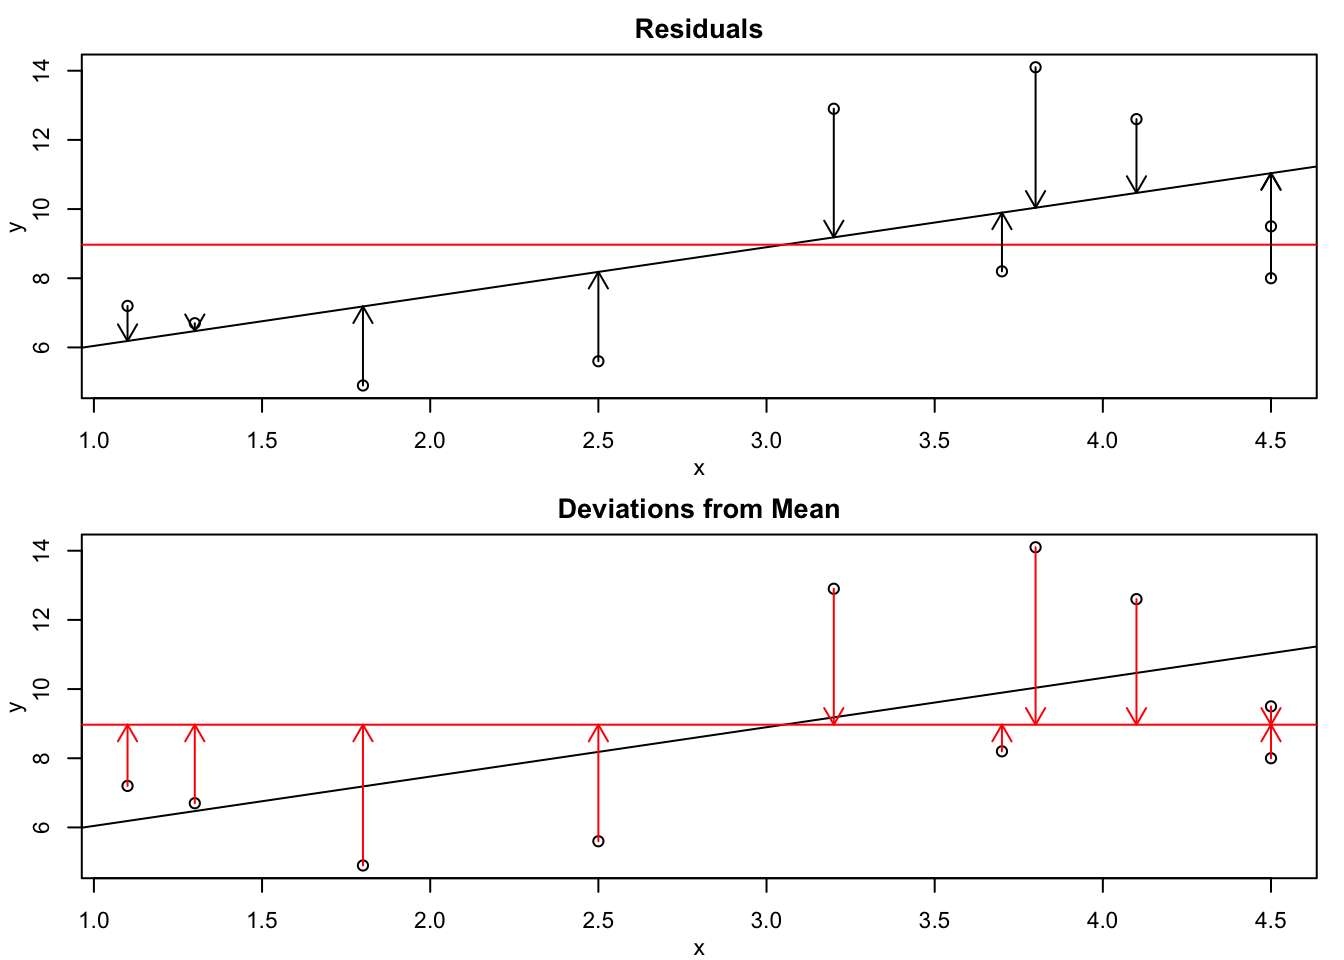
\includegraphics[width=0.6\linewidth]{statthink_files/figure-latex/Regression6-1} 

}

\caption{Residuals and Deviations from the Mean}\label{fig:Regression6}
\end{figure}

Consult the upper plot in Figure~\ref{fig:Regression6}. This is a
scatter plot of the data, together with the regression line in \emph{black}
and the line of the average in \emph{red}. A vertical arrow extends from each
data point to the regression line. The point where each arrow hits the
regression line is associated with the estimated value of the
expectation for that point. The residual is the difference between the
value of the response at the origin of the arrow and the value of the
response at the tip of its head. Notice that there are as many residuals
as there are observations.

The function ``\texttt{residuals}'' computes the residuals. The input to the
function is the fitted regression model and the output is the sequence
of residuals. When we apply the function to the object ``\texttt{fit}'', which
contains the fitted regression model for the fish data, we get the
residuals:

\begin{Shaded}
\begin{Highlighting}[]
\KeywordTok{residuals}\NormalTok{(fit)}
\end{Highlighting}
\end{Shaded}

\begin{verbatim}
##          1          2          3          4          5          6 
## -1.5397075 -1.6977999 -2.2857694  0.2279229  3.7158923  4.0594616 
##          7          8          9         10 
## -2.5849385 -3.0397075  2.1312463  1.0133998
\end{verbatim}

Indeed, 10 residuals are produced, one for each observation. In
particular, the residual for the first observation is -1.5397075, which
is essentially the value that we obtained\footnote{The discrepancy between the value that we computed and the value
  computed by the function results from rounding up errors. We used
  the vales of the coefficients that appear in the report. These
  values are rounded up. The function ``\texttt{residuals}'' uses the
  coefficients without rounding.}.

Return to the report produced by the application of the function
``\texttt{summary}'' to the fitted regression model. The first component in the
report is the formula that identifies the response and the explanatory
variable. The second component, the component that comes under the title
``\texttt{Residuals:}'', gives a summary of the distribution of the residuals.
This summary includes the smallest and the largest values in the
sequence of residuals, as well as the first and third quartiles and the
median. The average is not reported since the average of the residuals
from the regression line is always equal to 0.

The table that contains information on the coefficients was discussed in
the previous section. Let us consider the last 3 lines of the report.

The first of the three lines contains the estimated value of the
standard deviation of the response from the regression model. If the
expectations of the measurements of the response are located on the
regression line then the variability of the response corresponds to the
variability about this line. The resulting variance is estimated by the
sum of squares of the residuals from the regression line, divided by the
number of observations minus 2. A division by the number of observation
minus 2 produces an unbiased estimator of the variance of the response
about the regression model. Taking the square root of the estimated
variance produces an estimate of the standard deviation:

\begin{Shaded}
\begin{Highlighting}[]
\KeywordTok{sqrt}\NormalTok{(}\KeywordTok{sum}\NormalTok{(}\KeywordTok{residuals}\NormalTok{(fit)}\OperatorTok{^}\DecValTok{2}\NormalTok{)}\OperatorTok{/}\DecValTok{8}\NormalTok{)}
\end{Highlighting}
\end{Shaded}

\begin{verbatim}
## [1] 2.7907866
\end{verbatim}

The last computation is a manual computation of the estimated standard
deviation. It involves squaring the residuals and summing the squares.
This sum is divided by the number of observations minus 2 (\(10-2=8\)).
Taking the square root produces estimate. The value that we get for the
estimated standard deviation is 2.790787, which coincides with the value
that appears in the first of the last 3 lines of the report.

The second of these lines reports the R-squared of the linear fit. In
order to explain the meaning of R-squared let us consider
Figure~\ref{fig:Regression6} once again. The two plots in the figure
present the scatter plot of the data together with the regression line
and the line of the average. Vertical \emph{black} arrows that represent the
residuals from the regression are added to the upper plot. The lower
plot contains vertical \emph{red} arrows that extend from the data points to
the line of the average. These arrows represent the deviations of the
response from the average.

Consider two forms of variation. One form is the variation of the
response from its average value. This variation is summarized by the
sample variance, the sum of the squared lengths of the \emph{red} arrows
divided by the number of observations minus 1. The other form of
variation is the variation of the response from the fitted regression
line. This variation is summarized by the sample variation of the
residuals, the sum of squared lengths of the \emph{black} arrows divided by
the number of observations minus 1. The ratio between these two
quantities gives the relative variability of the response that remains
after fitting the regression line to the data.

The line of the average is a straight line. The deviations of the
observations from this straight line can be thought of as residuals from
that line. The variability of these residuals, the sum of squares of the
deviations from the average divided by the number of observations minus
1, is equal to the sample variance.

The regression line is the unique straight line that minimizes the
variability of its residuals. Consequently, the variability of the
residuals from the regression, the sum of squares of the residuals from
the regression divided by the number of observations minus 1, is the
smallest residual variability produced by any straight line. It follows
that the sample variance of the regression residuals is less than the
sample variance of the response. Therefore, the ratio between the
variance of the residuals and the variance of the response is less than
1.

R-squared is the difference between 1 and the ratio of the variances.
Its value is between 0 and 1 and it represents the fraction of the
variability of the response that is \emph{explained} by the regression line.
The closer the points are to the regression line the larger the value of
R-squared becomes. On the other hand, the less there is a linear trend
in the data the closer to 0 is the value of R-squared. In the extreme
case of R-squared equal to 1 all the data point are positioned exactly
on a single straight line. In the other extreme, a value of 0 for
R-squared implies no linear trend in the data.

Let us compte manually the difference between 1 and the ratio between
the variance of the residuals and the variance of the response:

\begin{Shaded}
\begin{Highlighting}[]
\DecValTok{1}\OperatorTok{-}\KeywordTok{var}\NormalTok{(}\KeywordTok{residuals}\NormalTok{(fit))}\OperatorTok{/}\KeywordTok{var}\NormalTok{(y)}
\end{Highlighting}
\end{Shaded}

\begin{verbatim}
## [1] 0.32974132
\end{verbatim}

Observe that the computed value of R-squared is the same as the value
``\texttt{Multiple\ R-squared:\ 0.3297}'' that is given in the report.

The report provides another value of R-squared, titled \emph{Adjusted
R-squared}. The difference between the adjusted and unadjusted
quantities is that in the former the sample variance of the residuals
from the regression is replaced by an unbiased estimate of the
variability of the response about the regression line. The sum of
squares in the unbiased estimator is divided by the number of
observations minus 2. Indeed, when we re-compute the ratio using the
unbiased estimate, the sum of squared residuals divided by \(10 - 2 = 8\),
we get:

\begin{Shaded}
\begin{Highlighting}[]
\DecValTok{1}\OperatorTok{-}\NormalTok{(}\KeywordTok{sum}\NormalTok{(}\KeywordTok{residuals}\NormalTok{(fit)}\OperatorTok{^}\DecValTok{2}\NormalTok{)}\OperatorTok{/}\DecValTok{8}\NormalTok{)}\OperatorTok{/}\KeywordTok{var}\NormalTok{(y)}
\end{Highlighting}
\end{Shaded}

\begin{verbatim}
## [1] 0.24595898
\end{verbatim}

The value of this adjusted quantity is equal to the value
``\texttt{Adjusted\ R-squared:\ 0.246}'' in the report.

Which value of R-squared to use is a matter of personal taste. In any
case, for a larger number of observations the difference between the two
values becomes negligible.

The last line in the report produces an overall goodness of fit test for
the regression model. In the current application of linear regression
this test reduces to a test of the slope being equal to zero, the same
test that is reported in the second row of the table of
coefficients\footnote{In more complex applications of linear regression, applications
  that are not considered in this book, the test in the last line of
  the report and the tests of coefficients do not coincide.}. The \(F\) statistic is simply the square of the \(t\)
value that is given in the second row of the table. The sampling
distribution of this statistic under the null hypothesis is the
\(F\)-distribution on 1 and \(n-2\) degrees of freedom, which is the
sampling distribution of the square of the test statistic for the slope.
The computed \(p\)-value, ``\texttt{p-value:\ 0.08255}'' is the identical (after
rounding up) to the \(p\)-value given in the second line of the table.

Return to the R-squared coefficient. This coefficient is a convenient
measure of the goodness of fit of the regression model to the data. Let
us demonstrate this point with the aid of the ``\texttt{cars}'' data. In
Subsection~\ref{subsec:Inference} we fitted a regression model to
the power of the engine as a response and the size of the engine as an
explanatory variable. The fitted model was saved in the object called
``\texttt{fit.power}''. A report of this fit, the output of the expression
``\texttt{summary(fit.power)}'' was also presented. The null hypothesis of zero
slope was clearly rejected. The value of R-squared for this fit was
0.6574. Consequently, about 2/3 of the variability in the power of the
engine is explained by the size of the engine.

Consider trying to fit a different regression model for the power of the
engine as a response. The variable ``\texttt{length}'' describes the length of
the car (in inches). How well would the length explain the power of the
car? We may examine this question using linear regression:

\begin{Shaded}
\begin{Highlighting}[]
\KeywordTok{summary}\NormalTok{(}\KeywordTok{lm}\NormalTok{(horsepower }\OperatorTok{~}\StringTok{ }\NormalTok{length, }\DataTypeTok{data=}\NormalTok{cars))}
\end{Highlighting}
\end{Shaded}

\begin{verbatim}
## 
## Call:
## lm(formula = horsepower ~ length, data = cars)
## 
## Residuals:
##      Min       1Q   Median       3Q      Max 
## -53.5706 -20.3471  -6.6903  14.4531 180.7167 
## 
## Coefficients:
##               Estimate Std. Error t value  Pr(>|t|)    
## (Intercept) -205.39710   32.81851 -6.2586 2.303e-09 ***
## length         1.77963    0.18814  9.4591 < 2.2e-16 ***
## ---
## Signif. codes:  0 '***' 0.001 '**' 0.01 '*' 0.05 '.' 0.1 ' ' 1
## 
## Residual standard error: 33.118 on 201 degrees of freedom
##   (2 observations deleted due to missingness)
## Multiple R-squared:  0.30803,    Adjusted R-squared:  0.30459 
## F-statistic: 89.474 on 1 and 201 DF,  p-value: < 2.22e-16
\end{verbatim}

We used one expression to fit the regression model to the data and to
summarize the outcome of the fit.

A scatter plot of the two variables together with the regression line may be produced
using the code:

\begin{Shaded}
\begin{Highlighting}[]
\KeywordTok{plot}\NormalTok{(horsepower }\OperatorTok{~}\StringTok{ }\NormalTok{length, }\DataTypeTok{data=}\NormalTok{cars)}
\KeywordTok{abline}\NormalTok{(}\KeywordTok{lm}\NormalTok{(horsepower }\OperatorTok{~}\StringTok{ }\NormalTok{length, }\DataTypeTok{data=}\NormalTok{cars))}
\end{Highlighting}
\end{Shaded}

\begin{center}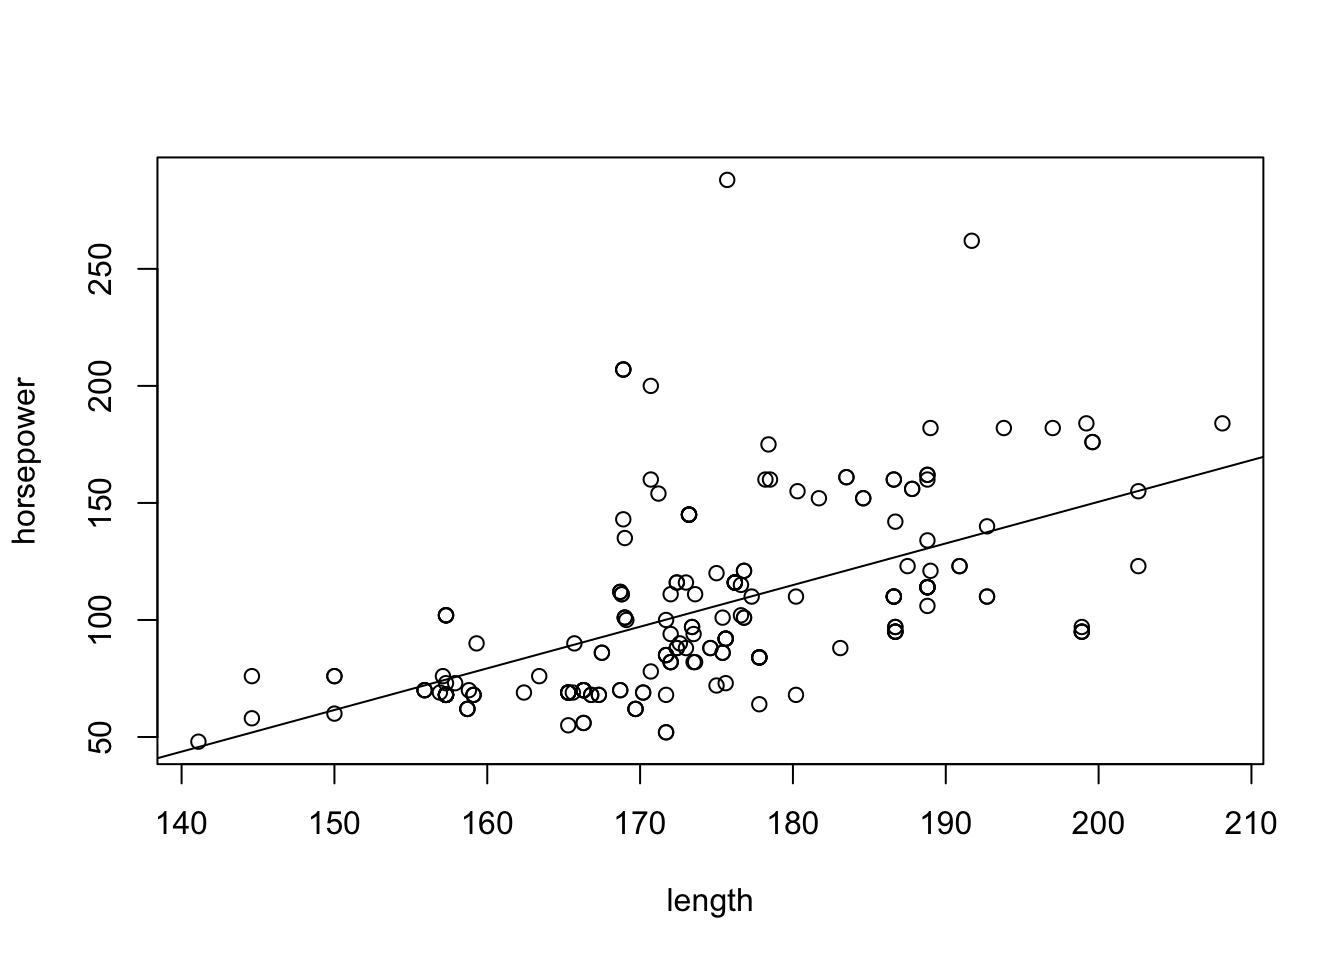
\includegraphics[width=0.6\linewidth]{statthink_files/figure-latex/unnamed-chunk-218-1} \end{center}

From the examination of the figure we may see that indeed there is a
linear trend in the relation between the length and the power of the
car. Longer cars tend to have more power. Testing the null hypothesis
that the slope is equal to zero produces a very small \(p\)-value and
leads to the rejection of the null hypothesis.

The length of the car and the size of the engine are both statistically
significant in their relation to the response. However, which of the two
explanatory variables produces a better fit?

An answer to this question may be provided by the examination of values
of R-squared, the ratio of the variance of the response explained by
each of the explanatory variable. The R-squared for the size of the
engine as an explanatory variable is 0.6574, which is approximately
equal to 2/3. The value of R-squared for the length of the car as an
explanatory variable is 0.308, less than 1/3. It follows that the size
of the engine explains twice as much of the variability of the power of
the engine than the size of car and is a better explanatory variable.

\hypertarget{exercises-9}{%
\section{Exercises}\label{exercises-9}}

\BeginKnitrBlock{exercise}
\protect\hypertarget{exr:unnamed-chunk-219}{}{\label{exr:unnamed-chunk-219} }Figure~\ref{fig:Regression8} presents 10 points and
three lines. One of the lines is colored \emph{red} and one of the points is
marked as a \emph{red triangle}. The points in the plot refer to the data
frame in Table~\[tab:Regression\_2\] and the three lines refer to the
linear equations:

\begin{enumerate}
\def\labelenumi{\arabic{enumi}.}
\item
  \(y = 4\)
\item
  \(y = 5 - 2x\)
\item
  \(y = x\)
\end{enumerate}

You are asked to match the marked line to the appropriate linear
equation and match the marked point to the appropriate observation:

\begin{enumerate}
\def\labelenumi{\arabic{enumi}.}
\item
  Which of the three equations, 1, 2 or 3, describes the line marked
  in \emph{red}?
\item
  The poind marked with a \emph{red triangle} represents which of the
  observations. (Identify the observation number.)
\end{enumerate}

\[tab:Regression\_2\]

\begin{longtable}[]{@{}crr@{}}
\caption{Points}\tabularnewline
\toprule
Observation & \(x\) & \(y\)\tabularnewline
\midrule
\endfirsthead
\toprule
Observation & \(x\) & \(y\)\tabularnewline
\midrule
\endhead
1 & 2.3 & -3.0\tabularnewline
2 & -1.9 & 9.8\tabularnewline
3 & 1.6 & 4.3\tabularnewline
4 & -1.6 & 8.2\tabularnewline
5 & 0.8 & 5.9\tabularnewline
6 & -1.0 & 4.3\tabularnewline
7 & -0.2 & 2.0\tabularnewline
8 & 2.4 & -4.7\tabularnewline
9 & 1.8 & 1.8\tabularnewline
10 & 1.4 & -1.1\tabularnewline
\bottomrule
\end{longtable}
\EndKnitrBlock{exercise}

\begin{figure}

{\centering 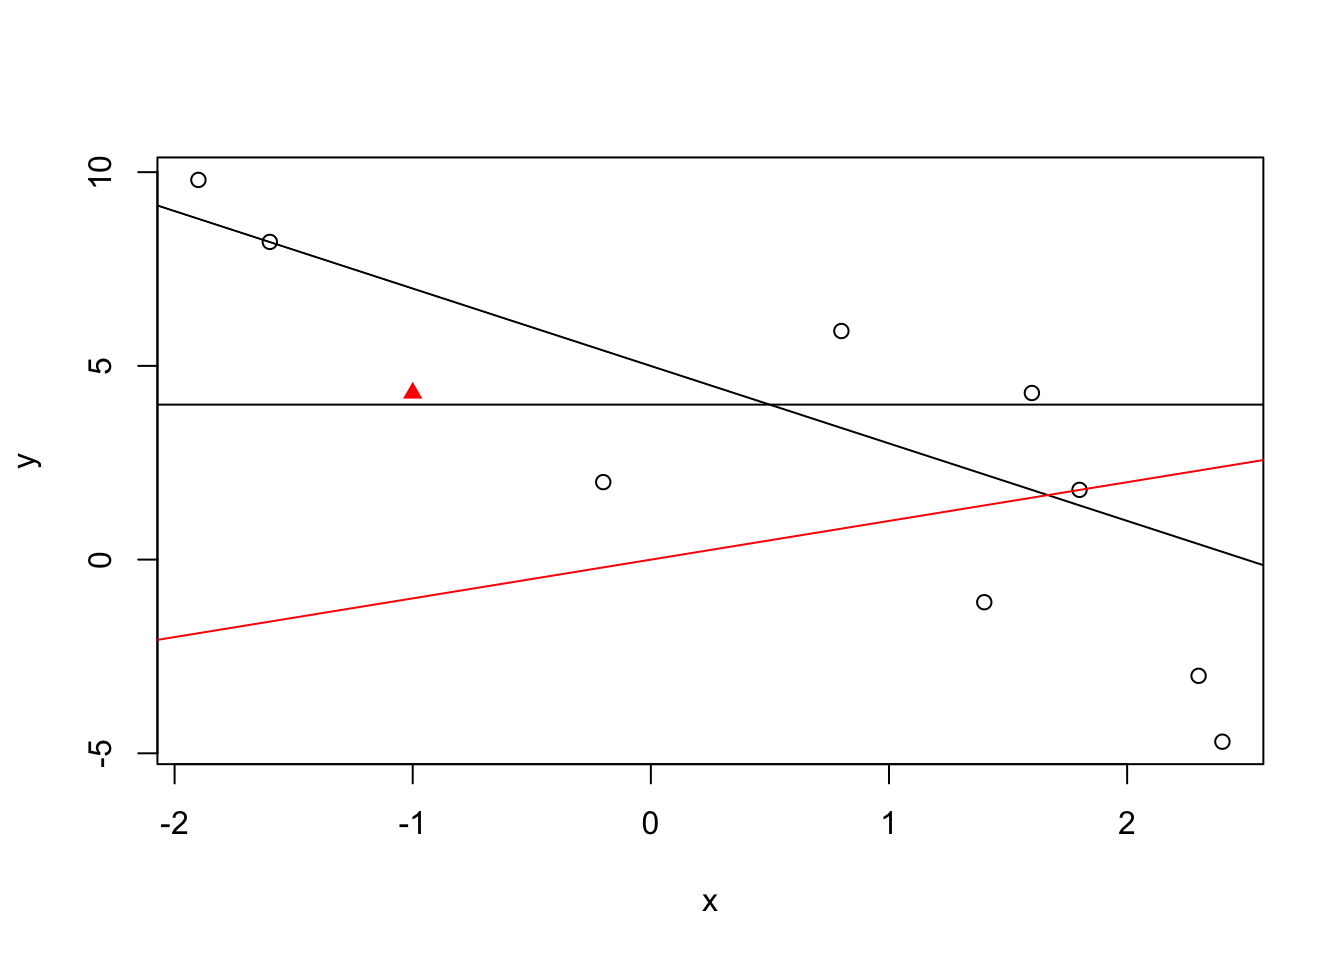
\includegraphics[width=0.6\linewidth]{statthink_files/figure-latex/Regression8-1} 

}

\caption{Lines and Points}\label{fig:Regression8}
\end{figure}

\BeginKnitrBlock{exercise}
\protect\hypertarget{exr:unnamed-chunk-220}{}{\label{exr:unnamed-chunk-220} }Assume a regression model that describes the
relation between the expectation of the response and the value of the
explanatory variable in the form:

\[\Expec(Y_i) = 2.13 \cdot x_i - 3.60\;.\]

\begin{enumerate}
\def\labelenumi{\arabic{enumi}.}
\item
  What is the value of the intercept and what is the value of the
  slope in the linear equation that describes the model?
\item
  Assume the \(x_1 = 5.5\), \(x_2 = 12.13\), \(x_3 = 4.2\), and \(x_4 = 6.7\).
  What is the expected value of the response of the 3rd observation?
\end{enumerate}
\EndKnitrBlock{exercise}

\BeginKnitrBlock{exercise}
\protect\hypertarget{exr:unnamed-chunk-221}{}{\label{exr:unnamed-chunk-221} }The file ``\texttt{aids.csv}'' contains data on the number of
diagnosed cases of Aids and the number of deaths associated with Aids
among adults and adolescents in the United States between 1981 and
2002\footnote{The data is taken from \href{http://cnx.org/content/m17088/latest/}{Table~1} in section ``Practice
  in Linear Regression'' of the online Textbook \href{http://cnx.org/content/col10522/1.38}{``Collaborative
  Statistics'' (Connexions. March 22, 2010.
  http://cnx.org/content/col10522/1.38/)}
  by Barbara Illowsky and Susan Dean.}. The file can be found on the internet at
\url{http://pluto.huji.ac.il/~msby/StatThink/Datasets/aids.csv}.

The file contains 3 variables: The variable ``\texttt{year}'' that tells the
relevant year, the variable ``\texttt{diagnosed}'' that reports the number of
Aids cases that were diagnosed in each year, and the variable ``\texttt{deaths}''
that reports the number of Aids related deaths in each year. The
following questions refer to the data in the file:

\begin{enumerate}
\def\labelenumi{\arabic{enumi}.}
\item
  Consider the variable ``\texttt{deaths}'' as response and the variable
  ``\texttt{diagnosed}'' as an explanatory variable. What is the slope of the
  regression line? Produce a point estimate and a confidence interval.
  Is it statistically significant (namely, significantly different
  than 0)?
\item
  Plot the scatter plot that is produced by these two variables and
  add the regression line to the plot. Does the regression line
  provided a good description of the trend in the data?
\item
  Consider the variable ``\texttt{diagnosed}'' as the response and the variable
  ``\texttt{year}'' as the explanatory variable. What is the slope of the
  regression line? Produce a point estimate and a confidence interval.
  Is the slope in this case statistically significant?
\item
  Plot the scatter plot that is produced by the later pair of
  variables and add the regression line to the plot. Does the
  regression line provided a good description of the trend in the
  data?
\end{enumerate}
\EndKnitrBlock{exercise}

\BeginKnitrBlock{exercise}
\protect\hypertarget{exr:unnamed-chunk-222}{}{\label{exr:unnamed-chunk-222} }Below are the percents of the U.S. labor force
(excluding self-employed and unemployed) that are members of a labor
union\footnote{Taken from \href{http://cnx.org/content/m17085/latest/}{Homework}
  section in the chapter on linear regression of the online Textbook
  \href{http://cnx.org/content/col10522/1.38}{``Collaborative Statistics'' (Connexions. March 22, 2010.
  http://cnx.org/content/col10522/1.38/)}
  by Barbara Illowsky and Susan Dean.}. We use this data in order to practice the computation of the
regression coefficients.

\[tab:Regression\_4\]

\begin{longtable}[]{@{}cr@{}}
\caption{Percent of Union Members}\tabularnewline
\toprule
year & percent\tabularnewline
\midrule
\endfirsthead
\toprule
year & percent\tabularnewline
\midrule
\endhead
1945 & 35.5\tabularnewline
1950 & 31.5\tabularnewline
1960 & 31.4\tabularnewline
1970 & 27.3\tabularnewline
1980 & 21.9\tabularnewline
1986 & 17.5\tabularnewline
1993 & 15.8\tabularnewline
\bottomrule
\end{longtable}

\begin{enumerate}
\def\labelenumi{\arabic{enumi}.}
\item
  Produce the scatter plot of the data and add the regression line. Is
  the regression model reasonable for this data?
\item
  Compute the sample averages and the sample standard deviations of
  both variables. Compute the covariance between the two variables.
\item
  Using the summaries you have just computed, recompute the
  coefficients of the regression model.
\end{enumerate}
\EndKnitrBlock{exercise}

\BeginKnitrBlock{exercise}
\protect\hypertarget{exr:unnamed-chunk-223}{}{\label{exr:unnamed-chunk-223} }Assume a regression model was fit to some data that
describes the relation between the explanatory variable \(x\) and the
response \(y\). Assume that the coefficients of the fitted model are
\(a=2.5\) and \(b=-1.13\), for the intercept and the slope, respectively.
The first 4 observations in the data are \((x_1,y_1) = (5.5,3.22)\),
\((x_2,y_2) = (12.13,-6.02)\), \((x_3,y_3) = (4.2,-8.3)\), and
\((x_4,y_4) = (6.7,0.17)\).

\begin{enumerate}
\def\labelenumi{\arabic{enumi}.}
\item
  What is the estimated expectation of the response for the 4th
  observation?
\item
  What is the residual from the regression line for the 4th
  observation?
\end{enumerate}
\EndKnitrBlock{exercise}

\BeginKnitrBlock{exercise}
\protect\hypertarget{exr:unnamed-chunk-224}{}{\label{exr:unnamed-chunk-224} }In Chapter~\ref{ChapTwoSamp} we analyzed an example
that involved the difference between fuel consumption in highway and
city driving conditions as the response\footnote{The response was computed using the expression
  ``\texttt{cars\$highway.mpg\ -\ cars\$city.mpg}''}. The explanatory variable
was a factor that was produced by splitting the cars into two weight
groups. In this exercise we would like to revisit this example. Here we
use the weight of the car directly as an explanatory variable. We also
consider the size of the engine as an alternative explanatory variable
and compare between the two regression models.

\begin{enumerate}
\def\labelenumi{\arabic{enumi}.}
\item
  Fit the regression model that uses the variable ``\texttt{curb.weight}'' as
  an explanatory variable. Is the slope significantly different than
  0? What fraction of the standard deviation of the response is
  explained by a regression model involving this variable?
\item
  Fit the regression model that uses the variable ``\texttt{engine.size}'' as
  an explanatory variable. Is the slope significantly different than
  0? What fraction of the standard deviation of the response is
  explained by a regression model involving this variable?
\item
  Which of the two models fits the data better?
\end{enumerate}
\EndKnitrBlock{exercise}

\hypertarget{summary-12}{%
\section{Summary}\label{summary-12}}

\hypertarget{glossary}{%
\subsection*{Glossary}\label{glossary}}


\begin{description}
\item[Regression:]
Relates different variables that are measured on the same sample.
Regression models are used to describe the effect of one of the
variables on the distribution of the other one. The former is called
the explanatory variable and the later is called the response.
\item[Linear Regression:]
The effect of a numeric explanatory variable on the distribution of
a numeric response is described in terms of a linear trend.
\item[Scatter Plot:]
A plot that presents the data in a pair of numeric variables. The
axes represents the variables and each point represents an
observation.
\item[Intercept:]
A coefficient of a linear equation. Equals the value of \(y\) when the
line crosses the \(y\)-axis.
\item[Slope:]
A coefficient of a linear equation. The change in the value of \(y\)
for each unit change in the value of \(x\). A positive slope
corresponds to an increasing line and a negative slope corresponds
to a decreasing line.
\item[Covariance:]
A measures the joint variability of two numeric variables. It is
equal to the sum of the product of the deviations from the mean,
divided by the number of observations minus 1.
\item[Residuals from Regression:]
The residual differences between the values of the response for the
observation and the estimated expectations of the response under the
regression model (the predicted response).
\item[R-Square:]
is the difference between 1 and the ratio between the variance of
the residuals from the regression and the variance of the response.
Its value is between 0 and 1 and it represents the fraction of the
variability of the response that is \emph{explained} by the regression
line.
\end{description}

\hypertarget{discuss-in-the-forum}{%
\subsection*{Discuss in the Forum}\label{discuss-in-the-forum}}


The topic for discussion in the Forum of Chapter~\ref{ChapNormal} was
mathematical models and how good they should fit reality. In this Forum
we would like to return to the same topic subject, but consider it
specifically in the context of statistical models.

Some statisticians prefer complex models, models that try to fit the
data as closely as one can. Others prefer a simple model. They claim
that although simpler models are more remote from the data yet they are
easier to interpret and thus provide more insight. What do you think?
Which type of model is better to use?

When formulating your answer to this question you may thing of a
situation that involves inference based on data conducted by yourself
for the sack of others. What would be the best way to report your
findings and explain them to the others?

\hypertarget{formulas}{%
\subsection*{Formulas:}\label{formulas}}


\begin{itemize}
\item
  A Linear Equation: \(y = a + b \cdot x\).
\item
  Covariance:
  \(\frac{\mbox{Sum of products of the deviations}}{\mbox{Number of values in the sample}-1} = \frac{\sum_{i=1}^n (y_i-\bar y)(x_i - \bar x)}{n-1}\).
\item
  Regression Slope: \(b = \mbox{Covariance}(x,y)/\mbox{Var}(x)\).
\item
  Regression Intercept: \(a = \bar y - b\bar x\).
\item
  The Regression Model: \(\Expec(Y_i) = a + b \cdot x_i\), \(a\) and \(b\)
  population parameters.
\item
  Residuals: \(y_i - (a + bx_i)\), \(a\) and \(b\) estimated from the data.
\item
  Estimate of Residual Variance:
  \(\sum_{i=1}^n(y_i - (a + bx_i))^2/(n-2)\), \(a\) and \(b\) estimated from
  the data.
\item
  R-Squared:
  \(1 - \sum_{i=1}^n(y_i - (a + bx_i))^2/\sum_{i=1}^n(y_i - \bar y)^2\),
  \(a\) and \(b\) estimated from the data.
\end{itemize}

\hypertarget{ChapLogistic}{%
\chapter{A Bernoulli Response}\label{ChapLogistic}}

\hypertarget{student-learning-objectives-9}{%
\section{Student Learning Objectives}\label{student-learning-objectives-9}}

Chapters~\ref{ChapTwoSamp} and~\ref{ChapRegression} introduced statistical
inference that involves a response and an explanatory variable that may
affect the distribution of the response. In both chapters the response
was numeric. The two chapters differed in the data type of the
explanatory variable. In Chapter~\ref{ChapTwoSamp} the explanatory variable
was a factor with two levels that splits the sample into two
sub-samples. In Chapter~\ref{ChapRegression} the explanatory variable was
numeric and produced, together with the response, a linear trend. The
aim in this chapter is to consider the case where the response is a
Bernoulli variable. Such a variable may emerge as the indicator of the
occurrence of an event associated with the response or as a factor with
two levels. The explanatory variable is a factor with two levels in one
case or a numerical variable in the other case.

Specifically, when the explanatory variable is a factor with two levels
then we may use the function ``\texttt{prop.test}''. This function was used in
Chapter~\ref{ChapTesting} for the analysis of the probability of an event
in a single sample. Here we use it in order to compare between two
sub-samples. This is similar to the way the function ``\texttt{t.test}'' was used
for a numeric response for both a single sample and for the comparison
between sub-samples. For the case where the explanatory variable is
numeric we may use the function ``\texttt{glm}'', acronym for \emph{Generalized Linear
Model}, in order to fit an appropriate regression model to the data.

By the end of this chapter, the student should be able to:

\begin{itemize}
\item
  Produce mosaic plots of the response and the explanatory variable.
\item
  Apply the function ``\texttt{prop.test}'' in order to compare the probability
  of an event between two sub-populations
\item
  Define the logistic regression model that relates the probability of
  an event in the response to a numeric explanatory variable.
\item
  Fit the logistic regression model to data using the function ``\texttt{glm}''
  and produce statistical inference on the fitted model.
\end{itemize}

\hypertarget{comparing-sample-proportions}{%
\section{Comparing Sample Proportions}\label{comparing-sample-proportions}}

In this chapter we deal with a Bernoulli response. Such a response has
two levels, ``\texttt{TRUE}'' or ``\texttt{FALSE}''\footnote{The levels are frequently coded as 1 or 0, ``success'' or ``failure'',
  or any other pair of levels.}, and may emerges as the indicator
of an event. Else, it may be associated with a factor with two levels
and correspond to the indication of one of the two levels. Such response
was considered in Chapters~\ref{ChapConfidence} and~\ref{ChapTesting} where
confidence intervals and tests for the probability of an event where
discussed in the context of a single sample. In this chapter we discuss
the investigation of relations between a response of this form and an
explanatory variable.

We start with the case where the explanatory variable is a factor that
has two levels. These levels correspond to two sub-populations (or two
settings). The aim of the analysis is to compare between the two
sub-populations (or between the two settings) the probability of the
even.

The discussion in this section is parallel to the discussion in
Section~\ref{sec:ComparingMeans}. That section considered the comparison of
the expectation of a numerical response between two sub-populations. We
denoted these sub-populations \(a\) and \(b\) with expectations
\(\Expec(X_a)\) and \(\Expec(X_b)\), respectively. The inference used the
average \(\bar X_a\), which was based on a sub-sample of size \(n_a\), and
the average \(\bar X_b\), which was based on the other sub-sample of size
\(n_b\). The sub-samples variances \(S^2_a\) and \(S^2_b\) participated in the
inference as well. The application of a test for the equality of the
expectations and a confidence interval where produced by the application
of the function ``\texttt{t.test}'' to the data.

The inference problem, which is considered in this chapter, involves an
event. This event is being examined in two different settings that
correspond to two different sub-population \(a\) and \(b\). Denote the
probabilities of the event in each of the sub-populations by \(p_a\) and
\(p_b\). Our concern is the statistical inference associated with the
comparison of these two probabilities to each other.

Natural estimators of the probabilities are \(\hat P_a\) and \(\hat P_b\),
the sub-samples proportions of occurrence of the event. These estimators
are used in order to carry out the inference. Specifically, we consider
here the construction of a confidence interval for the difference
\(p_a - p_b\) and a test of the hypothesis that the probabilities are
equal.

The methods for producing the confidence intervals for the difference
and for testing the null hypothesis that the difference is equal to zero
are similar is principle to the methods that were described in
Section~\[sec:TwoSamp\_3\] for making parallel inferences regarding the
relations between expectations. However, the derivations of the tools
that are used in the current situation are not identical to the
derivations of the tools that were used there. The main differences
between the two cases is the replacement of the sub-sample averages by
the sub-sample proportions, a difference in the way the standard
deviation of the statistics are estimated, and the application of a
continuity correction. We do not discuss in this chapter the theoretical
details associated with the derivations. Instead, we demonstrate the
application of the inference in an example.

The variable ``\texttt{num.of.doors}'' in the data frame ``\texttt{cars}'' describes the
number of doors a car has. This variable is a factor with two levels,
``\texttt{two}'' and ``\texttt{four}''. We treat this variable as a response and
investigate its relation to explanatory variables. In this section the
explanatory variable is a factor with two levels and in the next section
it is a numeric variable. Specifically, in this section we use the
factor ``\texttt{fuel.type}'' as the explanatory variable. Recall that this
variable identified the type of fuel, diesel or gas, that the car uses.
The aim of the analysis is to compare the proportion of cars with four
doors between cars that run on diesel and cars that run on gas.

Let us first summarize the data in a \(2 \times 2\) frequency table. The
function ``\texttt{table}'' may be used in order to produce such a table:

\begin{Shaded}
\begin{Highlighting}[]
\NormalTok{cars <-}\StringTok{ }\KeywordTok{read.csv}\NormalTok{(}\StringTok{"_data/cars.csv"}\NormalTok{)}
\KeywordTok{table}\NormalTok{(cars}\OperatorTok{$}\NormalTok{fuel.type,cars}\OperatorTok{$}\NormalTok{num.of.doors)}
\end{Highlighting}
\end{Shaded}

\begin{verbatim}
##         
##          four two
##   diesel   16   3
##   gas      98  86
\end{verbatim}

When the function ``\texttt{table}'' is applied to a combination of two factors
then the output is a table of joint frequencies. Each entry in the table
contains the frequency in the sample of the combination of levels, one
from each variable, that is associated with the entry. For example,
there are 16 cars in the data set that have the level ``\texttt{four}'' for the
variable ``\texttt{num.of.doors}'' and the level ``\texttt{diesel}'' for the variable
``\texttt{fuel.type}''. Likewise, there are 3 cars that are associated with the
combination ``\texttt{two}'' and ``\texttt{diesel}''. The total number of entries to the
table is \(16 + 3 + 98 + 86 = 203\), which is the number of cars in the
data set, minus the two missing values in the variable ``\texttt{num.of.doors}''.

A graphical representation of the relation between the two factors can
be obtained using a mosaic plot. This plot is produced when the input to
the function ``\texttt{plot}'' is a formula where both the response and the
explanatory variables are factors:

\begin{Shaded}
\begin{Highlighting}[]
\KeywordTok{plot}\NormalTok{(num.of.doors }\OperatorTok{~}\StringTok{ }\NormalTok{fuel.type,}\DataTypeTok{data=}\NormalTok{cars)}
\end{Highlighting}
\end{Shaded}

\begin{figure}

{\centering 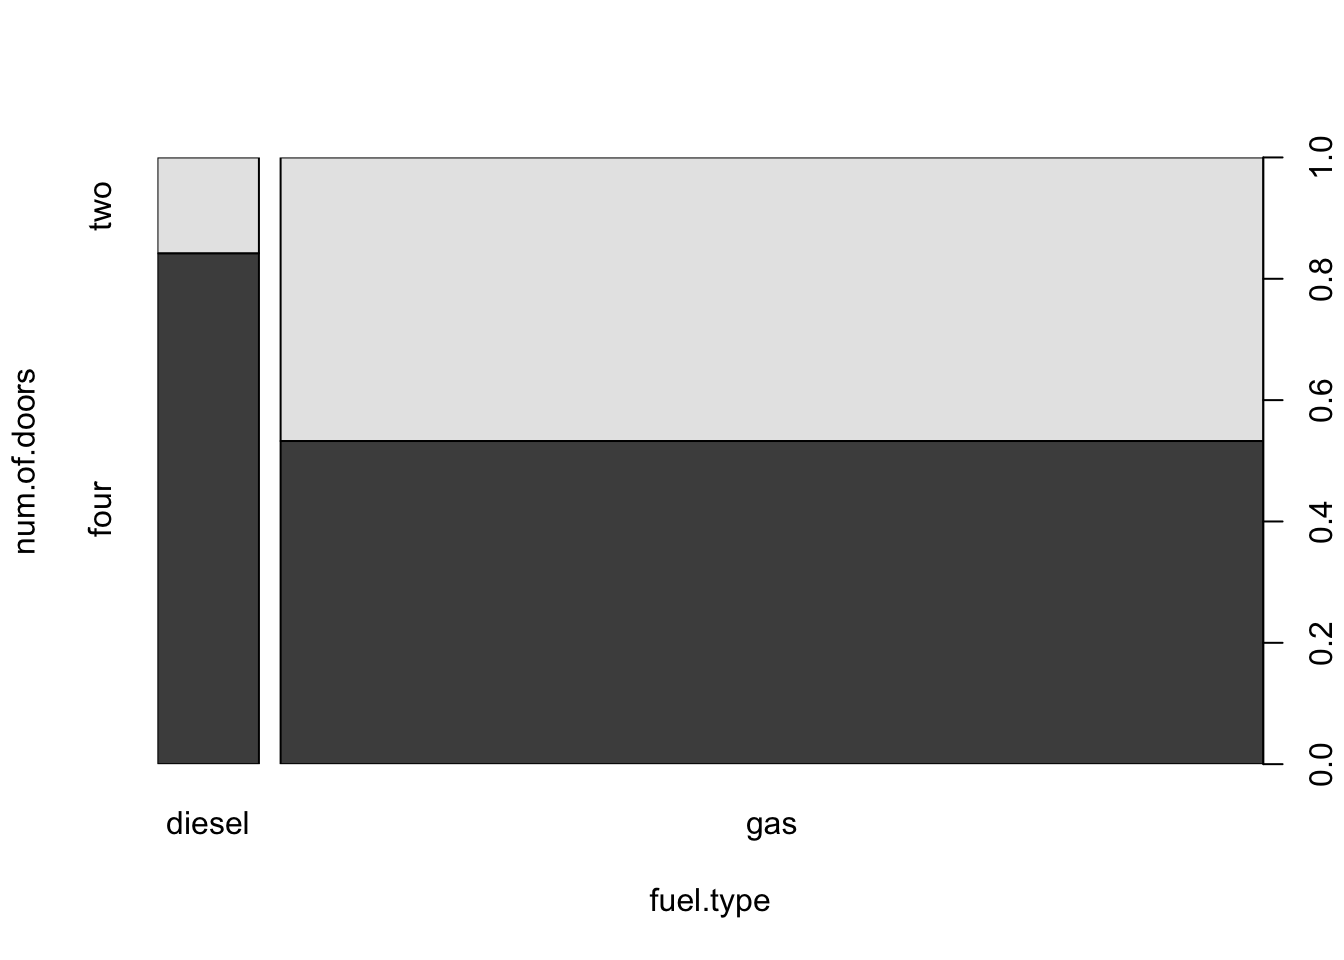
\includegraphics[width=0.6\linewidth]{statthink_files/figure-latex/Logistic1-1} 

}

\caption{Number of Doors versus Fuel Type}\label{fig:Logistic1}
\end{figure}

The box plot describes the distribution of the explanatory variable and
the distribution of the response for each level of the explanatory
variable. In the current example the explanatory variable is the factor
``\texttt{fuel}'' that has 2 levels. The two levels of this variable, ``\texttt{diesel}''
and ``\texttt{gas}'', are given at the \(x\)-axis. A vertical rectangle is
associated with each level. These 2 rectangles split the total area of
the square. The total area of the square represents the total relative
frequency (which is equal to 1). Consequently, the area of each
rectangle represents the relative frequency of the associated level of
the explanatory factor.

A rectangle associated with a given level of the explanatory variable is
further divided into horizontal sub-rectangles that are associated with
the response factor. In the current example each darker rectangle is
associated with the level ``\texttt{four}'' of the response ``\texttt{num.of.door}'' and
each brighter rectangle is associated with the level ``\texttt{two}''. The
relative area of the horizontal rectangles within each vertical
rectangle represent the relative frequency of the levels of the response
within each subset associated with the level of the explanatory
variable.

Looking at the plot one may appreciate the fact that diesel cars are
less frequent than cars that run on gas. The graph also displays the
fact that the relative frequency of cars with four doors among diesel
cars is larger than the relative frequency of four doors cars among cars
that run on gas.

The function ``\texttt{prop.test}'' may be used in order test the hypothesis
that, at the population level, the probability of the level ``four'' of
the response within the sub-population of diesel cars (the height of the
leftmost darker rectangle in the theoretic mosaic plot that is produced
for the entire population) is equal to the probability of the same level
of the response with in the sub-population of cars that run on gas (the
height of the rightmost darker rectangle in that theoretic mosaic plot).
Specifically, let us test the hypothesis that the two probabilities of
the level ``four'', one for diesel cars and one for cars that run on gas,
are equal to each other.

The output of the function ``\texttt{table}'' may serve as the input to the
function ``\texttt{prop.test}''\footnote{The function ``\texttt{prop.test}'' was applied in
  Section~\ref{TestFrac} in order to test that the probability of
  an event is equal to a given value (``\texttt{p\ =\ 0.5}'' by default). The
  input to the function was a pair of numbers: the total number of
  successes and the sample size. In the current application the input
  is a \(2 \times 2\) table. When applied to such input the function
  carries out a test of the equality of the probability of the first
  column between the rows of the table.}. The Bernoulli response variable should be
the second variable in the input to the table whereas the explanatory
factor is the first variable in the table. When we apply the test to the
data we get the report:

\begin{Shaded}
\begin{Highlighting}[]
\KeywordTok{prop.test}\NormalTok{(}\KeywordTok{table}\NormalTok{(cars}\OperatorTok{$}\NormalTok{fuel.type,cars}\OperatorTok{$}\NormalTok{num.of.doors))}
\end{Highlighting}
\end{Shaded}

\begin{verbatim}
## 
##  2-sample test for equality of proportions with continuity
##  correction
## 
## data:  table(cars$fuel.type, cars$num.of.doors)
## X-squared = 5.50206, df = 1, p-value = 0.018994
## alternative hypothesis: two.sided
## 95 percent confidence interval:
##  0.10135419 0.51763895
## sample estimates:
##     prop 1     prop 2 
## 0.84210526 0.53260870
\end{verbatim}

The two sample proportions of cars with four doors among diesel and gas
cars are presented at the bottom of the report and serve as estimates of
the sub-populations probabilities. Indeed, the relative frequency of
cars with four doors among diesel cars is equal to
\(\hat p_a = 16/(16+3) = 16/19 = 0.8421053\). Likewise, the relative
frequency of cars with four doors among cars that ran on gas is equal to
\(\hat p_b = 98/(98+86) = 98/184 = 0.5326087\). The confidence interval
for the difference in the probability of a car with four doors between
the two sub-populations, \(p_a - p_b\), is reported under the title
``\texttt{95\ percent\ confidence\ interval}'' and is given as
\([0.1013542, 0.5176389]\).

The null hypothesis, which is the subject of this test, is
\(H_0: p_a = p_b\). This hypothesis is tested against the two-sided
alternative hypothesis \(H_1: p_a \not = p_b\). The test itself is based
on a test statistic that obtains the value \texttt{X-squared\ =\ 5.5021}. This
test statistic corresponds essentially to the deviation between the
estimated value of the parameter (the difference in sub-sample
proportions of the event) and the theoretical value of the parameter
(\(p_a - p_b = 0\)). This deviation is divided by the estimated standard
deviation and the ratio is squared. The statistic itself is produced via
a continuity correction that makes its null distribution closer to the
limiting chi-square distribution on one degree of freedom. The \(p\)-value
is computed based on this limiting chi-square distribution.

Notice that the computed \(p\)-value is equal to \texttt{p-value\ =\ 0.01899}. This
value is smaller than 0.05. Consequently, the null hypothesis is
rejected at the 5\% significance level in favor of the alternative
hypothesis. This alternative hypothesis states that the sub-populations
probabilities are different from each other.

\hypertarget{logistic-regression}{%
\section{Logistic Regression}\label{logistic-regression}}

In the previous section we considered a Bernoulli response and a factor
with two levels as an explanatory variable. In this section we use a
numeric variable as the explanatory variable. The discussion in this
section is parallel to the discussion in Chapter~\[ch:Regression\] that
presented the topic of linear regression. However, since the response is
not of the same form, it is the indicator of a level of a factor and not
a regular numeric response, then the tools the are used are different.
Instead of using linear regression we use another type of regression
that is called \emph{Logistic Regression}.

Recall that linear regression involved fitting a straight line to the
scatter plot of data points. This line corresponds to the expectation of
the response as a function of the explanatory variable. The estimated
coefficients of this line are computed from the data and used for
inference.

In logistic regression, instead of the consideration of the expectation
of a numerical response, one considers the probability of an event
associated with the response. This probability is treated as a function
of the explanatory variable. Parameters that determine this function are
estimated from the data and are used for inference regarding the
relation between the explanatory variable and the response. Again, we do
not discuss the theoretical details involved in the derivation of
logistic regression. Instead, we apply the method to an example.

We consider the factor ``\texttt{num.of.doors}'' as the response and the
probability of a car with four doors as the probability of the response.
The length of the car will serve as the explanatory variable.
Measurements of lengths of the cars are stored in the variable
``\texttt{length}'' in the data frame ``\texttt{cars}''.

First, let us plot the relation between the response and the explanatory
variable:

\begin{Shaded}
\begin{Highlighting}[]
\KeywordTok{plot}\NormalTok{(num.of.doors }\OperatorTok{~}\StringTok{ }\NormalTok{length,}\DataTypeTok{data=}\NormalTok{cars)}
\end{Highlighting}
\end{Shaded}

\begin{figure}

{\centering 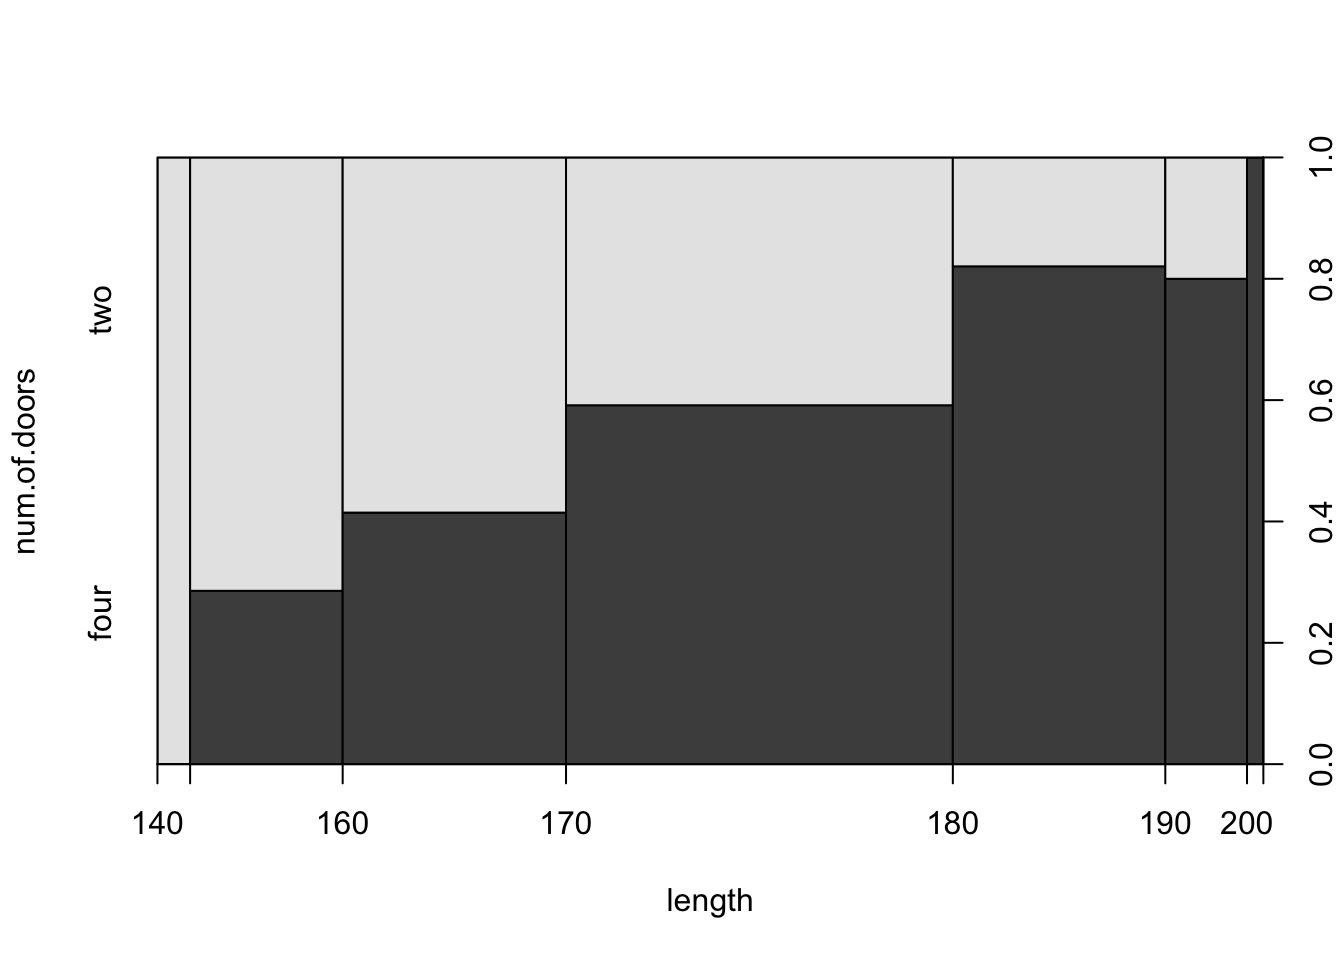
\includegraphics[width=0.6\linewidth]{statthink_files/figure-latex/Logistic2-1} 

}

\caption{Number of Doors versus Fuel Type}\label{fig:Logistic2}
\end{figure}

The plot is a type of a mosaic plot and it is
produced when the input to the function ``\texttt{plot}'' is a formula with a
factor as a response and a numeric variable as the explanatory variable.
The plot presents, for interval levels of the explanatory variable, the
relative frequencies of each interval. It also presents the relative
frequency of the levels of the response within each interval level of
the explanatory variable.

In order to get a better understanding of the meaning of the given
mosaic plot one may consider the histogram of the explanatory variable.

\begin{Shaded}
\begin{Highlighting}[]
\KeywordTok{hist}\NormalTok{(cars}\OperatorTok{$}\NormalTok{length)}
\end{Highlighting}
\end{Shaded}

\begin{figure}

{\centering \includegraphics[width=0.6\linewidth]{statthink_files/figure-latex/Logistic3-1} 

}

\caption{Histogram of the Length of Cars}\label{fig:Logistic3}
\end{figure}

The histogram
involves the partition of the range of variable length into intervals.
These interval are the basis for rectangles. The height of the
rectangles represent the frequency of cars with lengths that fall in the
given interval.

The mosaic plot in Figure~\ref{fig:Logistic2} is constructed on the
basis of this histogram. The \(x\)-axis in this plot corresponds to the
explanatory variable ``\texttt{length}''. The total area of the square in the
plot is divided between 7 vertical rectangles. These vertical rectangles
correspond to the 7 rectangles in the histogram of
Figure~\ref{fig:Logistic3}, turn on their sides. Hence, the width of
each rectangle in Figure~\ref{fig:Logistic2} correspond to the hight of
the parallel rectangle in the histogram. Consequently, the area of the
vertical rectangles in the mosaic plot represents the relative frequency
of the associated interval of values of the explanatory variable.

The rectangle that is associated with each interval of values of the
explanatory variable is further divided into horizontal sub-rectangles
that are associated with the response factor. In the current example
each darker rectangle is associated with the level ``\texttt{four}'' of the
response ``\texttt{num.of.door}'' and each brighter rectangle is associated with
the level ``\texttt{two}''. The relative area of the horizontal rectangles within
each vertical rectangle represent the relative frequency of the levels
of the response within each interval of values of the explanatory
variable.

From the examination of the mosaic plot one may identify relations
between the explanatory variable and the relative frequency of an
identified level of the response. In the current example one may observe
that the relative frequency of the cars with four doors is, overall,
increasing with the increase in the length of cars.

Logistic regression is a method for the investigation of relations
between the probability of an event and explanatory variables.
Specifically, we use it here for making inference on the number of doors
as a response and the length of the car as the explanatory variable.

Statistical inference requires a statistical model. The statistical
model in logistic regression relates the probability \(p_i\), the
probability of the event for observation \(i\), to \(x_i\), the value of the
response for that observation. The relation between the two in given by
the formula:

\[p_i = \frac{e^{a + b \cdot x_i}}{1 + e^{a + b\cdot x_i}}\;,\] where
\(a\) and \(b\) are coefficients common to all observations. Equivalently,
one may write the same relation in the form:

\[\log(p_i/[1-p_i]) = a + b\cdot x_i\;,\] that states that the relation
between a (function of) the probability of the event and the explanatory
variable is a linear trend.

One may fit the logistic regression to the data and test the null
hypothesis by the use of the function ``\texttt{glm}'':

\begin{Shaded}
\begin{Highlighting}[]
\NormalTok{fit.doors <-}\StringTok{ }\KeywordTok{glm}\NormalTok{(num.of.doors}\OperatorTok{==}\StringTok{"four"}\OperatorTok{~}\NormalTok{length, }\DataTypeTok{family=}\NormalTok{binomial,}\DataTypeTok{data=}\NormalTok{cars)}
\KeywordTok{summary}\NormalTok{(fit.doors)}
\end{Highlighting}
\end{Shaded}

\begin{verbatim}
## 
## Call:
## glm(formula = num.of.doors == "four" ~ length, family = binomial, 
##     data = cars)
## 
## Deviance Residuals: 
##      Min        1Q    Median        3Q       Max  
## -2.16459  -1.12916   0.56882   1.02401   1.66729  
## 
## Coefficients:
##               Estimate Std. Error z value  Pr(>|z|)    
## (Intercept) -13.147674   2.586929 -5.0823 3.728e-07 ***
## length        0.077256   0.014949  5.1681 2.365e-07 ***
## ---
## Signif. codes:  0 '***' 0.001 '**' 0.01 '*' 0.05 '.' 0.1 ' ' 1
## 
## (Dispersion parameter for binomial family taken to be 1)
## 
##     Null deviance: 278.331  on 202  degrees of freedom
## Residual deviance: 243.956  on 201  degrees of freedom
##   (2 observations deleted due to missingness)
## AIC: 247.956
## 
## Number of Fisher Scoring iterations: 3
\end{verbatim}

Generally, the function ``\texttt{glm}'' can be used in order to fit regression
models in cases where the distribution of the response has special
forms. Specifically, when the argument ``\texttt{family=binomial}'' is used then
the model that is being used in the model of logistic regression. The
formula that is used in the function involves a response and an
explanatory variable. The response may be a sequence with logical
``\texttt{TRUE}'' or ``\texttt{FALSE}'' values as in the example\footnote{The response is the output of the expression
  ``\texttt{num.of.doors==four}''. This expression produces logical values.
  ``\texttt{TRUE}'' when the car has 4 doors and ``\texttt{FALSE}'' when it has 2 doors.}. Alternatively, it
may be a sequence with ``1'' or ``0'' values, ``1'' corresponding to the event
occurring to the subject and ``0'' corresponding to the event not
occurring. The argument ``\texttt{data=cars}'' is used in order to inform the
function that the variables are located in the given data frame.

The ``\texttt{glm}'' function is applied to the data and the fitted model is
stored in the object ``\texttt{fit.doors}''.

A report is produced when the function ``\texttt{summary}'' is applied to the
fitted model. Notice the similarities and the differences between the
report presented here and the reports for linear regression that are
presented in Chapter~\ref{ChapRegression}. Both reports contain estimates
of the coefficients \(a\) and \(b\) and tests for the equality of these
coefficients to zero. When the coefficient \(b\), the coefficient that
represents the slope, is equal to 0 then the probability of the event
and the explanatory variable are unrelated. In the current case we may
note that the null hypothesis \(H_0: b = 0\), the hypothesis that claims
that there is no relation between the explanatory variable and the
response, is clearly rejected (\(p\)-value \(2.37 \times 10^{-7}\)).

The estimated values of the coefficients are \(-13.14767\) for the
intercept \(a\) and \(0.07726\) for the slope \(b\). One may produce
confidence intervals for these coefficients by the application of the
function ``\texttt{confint}'' to the fitted model:

\begin{Shaded}
\begin{Highlighting}[]
\KeywordTok{confint}\NormalTok{(fit.doors)}
\end{Highlighting}
\end{Shaded}

\begin{verbatim}
## Waiting for profiling to be done...
\end{verbatim}

\begin{verbatim}
##                    2.5 %      97.5 %
## (Intercept) -18.50384373 -8.31808771
## length        0.04938358  0.10824295
\end{verbatim}

\hypertarget{exercises-10}{%
\section{Exercises}\label{exercises-10}}

\BeginKnitrBlock{exercise}
\protect\hypertarget{exr:unnamed-chunk-229}{}{\label{exr:unnamed-chunk-229} }This exercise deals with a comparison between
Mediterranean diet and low-fat diet recommended by the American Heart
Association in the context of risks for illness or death among patients
that survived a heart attack\footnote{De Lorgeril, M., Salen, P., Martin, J., Monjaud, I., Boucher, P.,
  Mamelle, N. (1998). Mediterranean Dietary pattern in a Randomized
  Trial. Archives of Internal Medicine, 158, 1181-1187.}. This case study is taken from the
\href{http://onlinestatbook.com/rvls.html}{Rice Virtual Lab in Statistics}.
More details on this case study can be found in the case study
``\href{http://onlinestatbook.com/case_studies_rvls/diet_study/index.html}{Mediterranean Diet and
Health}''
that is presented in that site.

The subjects, 605 survivors of a heart attack, were randomly assigned
follow either (1) a diet close to the ``prudent diet step 1'' of the
American Heart Association (AHA) or (2) a Mediterranean-type diet
consisting of more bread and cereals, more fresh fruit and vegetables,
more grains, more fish, fewer delicatessen food, less meat.

The subjects` diet and health condition were monitored over a period of
four-year. Information regarding deaths, development of cancer or the
development of non-fatal illnesses was collected. The information from
this study is stored in the file ``\texttt{diet.csv}''. The file ``\texttt{diet.csv}''
contains two factors: ``\texttt{health}'' that describes the condition of the
subject, either healthy, suffering from a non-fatal illness, suffering
from cancer, or dead; and the ``\texttt{type}'' that describes the type of diet,
either Mediterranean or the diet recommended by the AHA. The file can be
found on the internet at
\url{http://pluto.huji.ac.il/~msby/StatThink/Datasets/diet.csv}. Answer the
following questions based on the data in the file:

\begin{enumerate}
\def\labelenumi{\arabic{enumi}.}
\item
  Produce a frequency table of the two variable. Read off from the
  table the number of healthy subjects that are using the
  Mediterranean diet and the number of healthy subjects that are using
  the diet recommended by the AHA.
\item
  Test the null hypothesis that the probability of keeping healthy
  following an heart attack is the same for those that use the
  Mediterranean diet and for those that use the diet recommended by
  the AHA. Use a two-sided alternative and a 5\% significance level.
\item
  Compute a 95\% confidence interval for the difference between the two
  probabilities of keeping healthy.
\end{enumerate}
\EndKnitrBlock{exercise}

\BeginKnitrBlock{exercise}
\protect\hypertarget{exr:unnamed-chunk-230}{}{\label{exr:unnamed-chunk-230} }Cushing's syndrome disorder results from a tumor
(adenoma) in the pituitary gland that causes the production of high
levels of cortisol. The symptoms of the syndrome are the consequence of
the elevated levels of this steroid hormone in the blood. The syndrome
was first described by Harvey Cushing in 1932.

The file ``\texttt{coshings.csv"} contains information on 27 patients that
suffer from Cushing's syndrome\footnote{The source of the data is the data file ``\texttt{Cushings}'' from the
  package ``\texttt{MASS}'' in \texttt{R}.}. The three variables in the file are
``\texttt{tetra}'', ``\texttt{pregn}'', and ``\texttt{type}''. The factor ``\texttt{type}'' describes the
underlying type of syndrome, coded as ``\texttt{a}``, (adenoma),''\texttt{b}" (bilateral
hyperplasia), ``\texttt{c}'' (carcinoma) or ``\texttt{u}'' for unknown. The variable
``\texttt{tetra}'' describe the level of urinary excretion rate (mg/24hr) of
Tetrahydrocortisone, a type of steroid, and the variable ``\texttt{pregn}''
describes urinary excretion rate (mg/24hr) of Pregnanetriol, another
type of steroid. The file can be found on the internet at
\url{http://pluto.huji.ac.il/~msby/StatThink/Datasets/coshings.csv}. Answer
the following questions based on the information in this file:

\begin{enumerate}
\def\labelenumi{\arabic{enumi}.}
\item
  Plot the histogram of the variable ``\texttt{tetra}'' and the mosaic plot
  that describes the relation between the variable ``\texttt{type}'' as a
  response and the variable ``\texttt{tetra}''. What is the information that is
  conveyed by the second vertical triangle from the right (the third
  from the left) in the mosaic plot.
\item
  Test the null hypothesis that there is no relation between the
  variable ``\texttt{tetra}'' as an explanatory variable and the indicator of
  the type being equal to ``\texttt{b}'' as a response. Compute a confidence
  interval for the parameter that describes the relation.
\item
  Repeat the analysis from 2 using only the observations for which the
  type is known. (Hint: you may fit the model to the required subset
  by the inclusion of the argument ``\texttt{subset=(type!=u)}'' in the
  function that fits the model.) Which of the analysis do you think is
  more appropriate?
\end{enumerate}
\EndKnitrBlock{exercise}

\hypertarget{glossary}{%
\subsection*{Glossary}\label{glossary}}


\begin{description}
\item[Mosaic Plot:]
A plot that describes the relation between a response factor and an
explanatory variable. Vertical rectangles represent the distribution
of the explanatory variable. Horizontal rectangles within the
vertical ones represent the distribution of the response.
\item[Logistic Regression:]
A type of regression that relates between an explanatory variable
and a response of the form of an indicator of an event.
\end{description}

\hypertarget{discuss-in-the-forum}{%
\subsection*{Discuss in the forum}\label{discuss-in-the-forum}}


In the description of the statistical models that relate one variable to
the other we used terms that suggest a causality relation. One variable
was called the ``explanatory variable'' and the other was called the
``response''. One may get the impression that the explanatory variable is
the cause for the statistical behavior of the response. In negation to
this interpretation, some say that all that statistics does is to
examine the joint distribution of the variables, but casuality cannot be
inferred from the fact that two variables are statistically related.
What do you think? Can statistical reasoning be used in the
determination of casuality?

As part of your answer in may be useful to consider a specific situation
where the determination of casuality is required. Can any of the tools
that were discussed in the book be used in a meaningful way to aid in
the process of such determination?

Notice that the last 3 chapters dealt with statistical models that
related an explanatory variable to a response. We considered tools that
can be used when both variable are factors and when both are numeric.
Other tools may be used when one of the variables is a factor and the
other is numeric. An analysis that involves one variable as the response
and the other as explanatory variable can be reversed, possibly using a
different statistical tool, with the roles of the variables exchanged.
Usually, a significant statistical finding will be still significant
when the roles of a response and an explanatory variable are reversed.

\hypertarget{formulas}{%
\subsection*{Formulas:}\label{formulas}}


\begin{itemize}
\item
  Logistic Regression, (Probability):
  \(p_i = \frac{e^{a + b \cdot x_i}}{1 + e^{a + b\cdot x_i}}\).
\item
  Logistic Regression, (Predictor):
  \(\log(p_i/[1-p_i]) = a + b\cdot x_i\).
\end{itemize}

\hypertarget{ChapCaseStudies}{%
\chapter{Case Studies}\label{ChapCaseStudies}}

\hypertarget{student-learning-objective-5}{%
\section{Student Learning Objective}\label{student-learning-objective-5}}

This chapter concludes this book. We start with a short review of the
topics that were discussed in the second part of the book, the part that
dealt with statistical inference. The main part of the chapter involves
the statistical analysis of 2 case studies. The tools that will be used
for the analysis are those that were discussed in the book. We close
this chapter and this book with some concluding remarks. By the end of
this chapter, the student should be able to:

\begin{itemize}
\item
  Review the concepts and methods for statistical inference that were
  presented in the second part of the book.
\item
  Apply these methods to requirements of the analysis of real data.
\item
  Develop a resolve to learn more statistics.
\end{itemize}

\hypertarget{a-review}{%
\section{A Review}\label{a-review}}

The second part of the book dealt with statistical inference; the
science of making general statement on an entire population on the basis
of data from a sample. The basis for the statements are theoretical
models that produce the sampling distribution. Procedures for making the
inference are evaluated based on their properties in the context of this
sampling distribution. Procedures with desirable properties are applied
to the data. One may attach to the output of this application summaries
that describe these theoretical properties.

In particular, we dealt with two forms of making inference. One form was
estimation and the other was hypothesis testing. The goal in estimation
is to determine the value of a parameter in the population. Point
estimates or confidence intervals may be used in order to fulfill this
goal. The properties of point estimators may be assessed using the mean
square error (MSE) and the properties of the confidence interval may be
assessed using the confidence level.

The target in hypotheses testing is to decide between two competing
hypothesis. These hypotheses are formulated in terms of population
parameters. The decision rule is called a statistical test and is
constructed with the aid of a test statistic and a rejection region. The
default hypothesis among the two, is rejected if the test statistic
falls in the rejection region. The major property a test must possess is
a bound on the probability of a Type I error, the probability of
erroneously rejecting the null hypothesis. This restriction is called
the significance level of the test. A test may also be assessed in terms
of it's statistical power, the probability of rightfully rejecting the
null hypothesis.

Estimation and testing were applied in the context of single
measurements and for the investigation of the relations between a pair
of measurements. For single measurements we considered both numeric
variables and factors. For numeric variables one may attempt to conduct
inference on the expectation and/or the variance. For factors we
considered the estimation of the probability of obtaining a level, or,
more generally, the probability of the occurrence of an event.

We introduced statistical models that may be used to describe the
relations between variables. One of the variables was designated as the
response. The other variable, the explanatory variable, is identified as
a variable which may affect the distribution of the response.
Specifically, we considered numeric variables and factors that have two
levels. If the explanatory variable is a factor with two levels then the
analysis reduces to the comparison of two sub-populations, each one
associated with a level. If the explanatory variable is numeric then a
regression model may be applied, either linear or logistic regression,
depending on the type of the response.

The foundations of statistical inference are the assumption that we make
in the form of statistical models. These models attempt to reflect
reality. However, one is advised to apply healthy skepticism when using
the models. First, one should be aware what the assumptions are. Then
one should ask oneself how reasonable are these assumption in the
context of the specific analysis. Finally, one should check as much as
one can the validity of the assumptions in light of the information at
hand. It is useful to plot the data and compare the plot to the
assumptions of the model.

\hypertarget{case-studies}{%
\section{Case Studies}\label{case-studies}}

Let us apply the methods that were introduced throughout the book to two
examples of data analysis. Both examples are taken from the case studies
of the \href{http://onlinestatbook.com/rvls.html}{Rice Virtual Lab in
Statistics} can be found in their
\href{http://onlinestatbook.com/case_studies_rvls/}{Case Studies} section.
The analysis of these case studies may involve any of the tools that
were described in the second part of the book (and some from the first
part). It may be useful to read again
Chapters~\ref{ChapInference}--\ref{ChapLogistic} before reading the case
studies.

\hypertarget{physicians-reactions-to-the-size-of-a-patient}{%
\subsection{Physicians' Reactions to the Size of a Patient}\label{physicians-reactions-to-the-size-of-a-patient}}

Overweight and obesity is common in many of the developed contrives. In
some cultures, obese individuals face discrimination in employment,
education, and relationship contexts. The current research, conducted by
Mikki Hebl and Jingping Xu\footnote{Hebl, M. and Xu, J. (2001). Weighing the care: Physicians'
  reactions to the size of a patient. International Journal of
  Obesity, 25, 1246-1252.}, examines physicians' attitude toward
overweight and obese patients in comparison to their attitude toward
patients who are not overweight.

The experiment included a total of 122 primary care physicians
affiliated with one of three major hospitals in the Texas Medical Center
of Houston. These physicians were sent a packet containing a medical
chart similar to the one they view upon seeing a patient. This chart
portrayed a patient who was displaying symptoms of a migraine headache
but was otherwise healthy. Two variables (the gender and the weight of
the patient) were manipulated across six different versions of the
medical charts. The weight of the patient, described in terms of Body
Mass Index (BMI), was average (BMI = 23), overweight (BMI = 30), or
obese (BMI = 36). Physicians were randomly assigned to receive one of
the six charts, and were asked to look over the chart carefully and
complete two medical forms. The first form asked physicians which of 42
tests they would recommend giving to the patient. The second form asked
physicians to indicate how much time they believed they would spend with
the patient, and to describe the reactions that they would have toward
this patient.

In this presentation, only the question on how much time the physicians
believed they would spend with the patient is analyzed. Although three
patient weight conditions were used in the study (average, overweight,
and obese) only the average and overweight conditions will be analyzed.
Therefore, there are two levels of patient weight (average and
overweight) and one dependent variable (time spent).

The data for the given collection of responses from 72 primary care
physicians is stored in the file ``\texttt{discriminate.csv}''\footnote{The file can be found on the internet at
  \url{http://pluto.huji.ac.il/~msby/StatThink/Datasets/discriminate.csv}.}. We start by
reading the content of the file into a data frame by the name
``\texttt{patient}'' and presenting the summary of the variables:

\begin{Shaded}
\begin{Highlighting}[]
\NormalTok{patient <-}\StringTok{ }\KeywordTok{read.csv}\NormalTok{(}\StringTok{"_data/discriminate.csv"}\NormalTok{)}
\KeywordTok{summary}\NormalTok{(patient)}
\end{Highlighting}
\end{Shaded}

\begin{verbatim}
##     weight        time       
##  BMI=23:33   Min.   : 5.000  
##  BMI=30:38   1st Qu.:20.000  
##              Median :30.000  
##              Mean   :27.817  
##              3rd Qu.:30.000  
##              Max.   :60.000
\end{verbatim}

Observe that of the 72 ``patients'', 38 are overweight and 33 have an
average weight. The time spend with the patient, as predicted by
physicians, is distributed between 5 minutes and 1 hour, with a average
of 27.82 minutes and a median of 30 minutes.

It is a good practice to have a look at the data before doing the
analysis. In this examination on should see that the numbers make sense
and one should identify special features of the data. Even in this very
simple example we may want to have a look at the histogram of the
variable ``\texttt{time}'':

\begin{Shaded}
\begin{Highlighting}[]
\KeywordTok{hist}\NormalTok{(patient}\OperatorTok{$}\NormalTok{time)}
\end{Highlighting}
\end{Shaded}

\begin{center}\includegraphics[width=0.6\linewidth]{statthink_files/figure-latex/unnamed-chunk-232-1} \end{center}

A feature in this plot that catches
attention is the fact that there is a high concventration of values in
the interval between 25 and 30. Together with the fact that the median
is equal to 30, one may suspect that, as a matter of fact, a large
numeber of the values are actually equal to 30. Indeed, let us produce a
table of the response:

\begin{Shaded}
\begin{Highlighting}[]
\KeywordTok{table}\NormalTok{(patient}\OperatorTok{$}\NormalTok{time)}
\end{Highlighting}
\end{Shaded}

\begin{verbatim}
## 
##  5 15 20 25 30 40 45 50 60 
##  1 10 15  3 30  4  5  2  1
\end{verbatim}

Notice that 30 of the 72 physicians marked ``\texttt{30}'' as the time they
expect to spend with the patient. This is the middle value in the range,
and may just be the default value one marks if one just needs to
complete a form and do not really place much importance to the question
that was asked.

The goal of the analysis is to examine the relation between overweigh
and the Doctor's response. The explanatory variable is a factor with two
levels. The response is numeric. A natural tool to use in order to test
this hypothesis is the \(t\)-test, which is implemented with the function
``\texttt{t.test}''.

First we plot the relation between the response and the explanatory
variable and then we apply the test:

\begin{Shaded}
\begin{Highlighting}[]
\KeywordTok{boxplot}\NormalTok{(time}\OperatorTok{~}\NormalTok{weight,}\DataTypeTok{data=}\NormalTok{patient)}
\end{Highlighting}
\end{Shaded}

\begin{center}\includegraphics[width=0.6\linewidth]{statthink_files/figure-latex/unnamed-chunk-234-1} \end{center}

\begin{Shaded}
\begin{Highlighting}[]
\KeywordTok{t.test}\NormalTok{(time}\OperatorTok{~}\NormalTok{weight,}\DataTypeTok{data=}\NormalTok{patient)}
\end{Highlighting}
\end{Shaded}

\begin{verbatim}
## 
##  Welch Two Sample t-test
## 
## data:  time by weight
## t = 2.85161, df = 67.1743, p-value = 0.0057739
## alternative hypothesis: true difference in means is not equal to 0
## 95 percent confidence interval:
##   1.9885321 11.2650564
## sample estimates:
## mean in group BMI=23 mean in group BMI=30 
##            31.363636            24.736842
\end{verbatim}

Nothing seems problematic in the box plot.
The two distributions, as they are reflected in the box plots, look
fairly symmetric.

When we consider the report that produced by the function ``\texttt{t.test}'' we
may observe that the \(p\)-value is equal to 0.005774. This \(p\)-value is
computed in testing the null hypothesis that the expectation of the
response for both types of patients are equal against the two sided
alternative. Since the \(p\)-value is less than 0.05 we do reject the null
hypothesis.

The estimated value of the difference between the expectation of the
response for a patient with BMI=23 and a patient with BMI=30 is
\(31.36364 -24.73684 \approx 6.63\) minutes. The confidence interval is
(approximately) equal to \([1.99, 11.27]\). Hence, it looks as if the
physicians expect to spend more time with the average weight patients.

After analyzing the effect of the explanatory variable on the
expectation of the response one may want to examine the presence, or
lack thereof, of such effect on the variance of the response. Towards
that end, one may use the function ``\texttt{var.test}'':

\begin{Shaded}
\begin{Highlighting}[]
\KeywordTok{var.test}\NormalTok{(time}\OperatorTok{~}\NormalTok{weight,}\DataTypeTok{data=}\NormalTok{patient)}
\end{Highlighting}
\end{Shaded}

\begin{verbatim}
## 
##  F test to compare two variances
## 
## data:  time by weight
## F = 1.04432, num df = 32, denom df = 37, p-value = 0.89306
## alternative hypothesis: true ratio of variances is not equal to 1
## 95 percent confidence interval:
##  0.53334055 2.07972695
## sample estimates:
## ratio of variances 
##           1.044316
\end{verbatim}

In this test we do not reject the null hypothesis that the two variances
of the response are equal since the \(p\)-value is larger than \(0.05\). The
sample variances are almost equal to each other (their ratio is
\(1.044316\)), with a confidence interval for the ration that essentially
ranges between 1/2 and 2.

The production of \(p\)-values and confidence intervals is just one aspect
in the analysis of data. Another aspect, which typically is much more
time consuming and requires experience and healthy skepticism is the
examination of the assumptions that are used in order to produce the
\(p\)-values and the confidence intervals. A clear violation of the
assumptions may warn the statistician that perhaps the computed nominal
quantities do not represent the actual statistical properties of the
tools that were applied.

In this case, we have noticed the high concentration of the response at
the value ``\texttt{30}''. What is the situation when we split the sample between
the two levels of the explanatory variable? Let us apply the function
``\texttt{table}'' once more, this time with the explanatory variable included:

\begin{Shaded}
\begin{Highlighting}[]
\KeywordTok{table}\NormalTok{(patient}\OperatorTok{$}\NormalTok{time,patient}\OperatorTok{$}\NormalTok{weight)}
\end{Highlighting}
\end{Shaded}

\begin{verbatim}
##     
##      BMI=23 BMI=30
##   5       0      1
##   15      2      8
##   20      6      9
##   25      1      2
##   30     14     16
##   40      4      0
##   45      4      1
##   50      2      0
##   60      0      1
\end{verbatim}

Not surprisingly, there is still high concentration at that level
``\texttt{30}''. But one can see that only 2 of the responses of the ``\texttt{BMI=30}''
group are above that value in comparison to a much more symmetric
distribution of responses for the other group.

The simulations of the significance level of the one-sample \(t\)-test for
an Exponential response that were conducted in Question~\[ex:Testing.2\]
may cast some doubt on how trustworthy are nominal \(p\)-values of the
\(t\)-test when the measurements are skewed. The skewness of the response
for the group ``\texttt{BMI=30}'' is a reason to be worry.

We may consider a different test, which is more robust, in order to
validate the significance of our findings. For example, we may turn the
response into a factor by setting a level for values larger or equal to
``\texttt{30}'' and a different level for values less than ``\texttt{30}''. The relation
between the new response and the explanatory variable can be examined
with the function ``\texttt{prop.test}''. We first plot and then test:

\begin{Shaded}
\begin{Highlighting}[]
\KeywordTok{plot}\NormalTok{(}\KeywordTok{factor}\NormalTok{(patient}\OperatorTok{$}\NormalTok{time}\OperatorTok{>=}\DecValTok{30}\NormalTok{)}\OperatorTok{~}\NormalTok{weight,}\DataTypeTok{data=}\NormalTok{patient)}
\end{Highlighting}
\end{Shaded}

\begin{center}\includegraphics[width=0.6\linewidth]{statthink_files/figure-latex/unnamed-chunk-237-1} \end{center}

\begin{Shaded}
\begin{Highlighting}[]
\KeywordTok{prop.test}\NormalTok{(}\KeywordTok{table}\NormalTok{(patient}\OperatorTok{$}\NormalTok{time}\OperatorTok{>=}\DecValTok{30}\NormalTok{,patient}\OperatorTok{$}\NormalTok{weight))}
\end{Highlighting}
\end{Shaded}

\begin{verbatim}
## 
##  2-sample test for equality of proportions with continuity
##  correction
## 
## data:  table(patient$time >= 30, patient$weight)
## X-squared = 3.7098, df = 1, p-value = 0.054094
## alternative hypothesis: two.sided
## 95 percent confidence interval:
##  -0.5155087984 -0.0066586892
## sample estimates:
##     prop 1     prop 2 
## 0.31034483 0.57142857
\end{verbatim}

The mosaic plot presents the relation between the explanatory
variable and the new factor.
The level ``\texttt{TRUE}'' is associated with a value of the predicted time
spent with the patient being 30 minutes or more. The level ``\texttt{FALSE}'' is
associated with a prediction of less than 30 minutes.

The computed \(p\)-value is equal to \(0.05409\), that almost reaches the
significance level of 5\%\footnote{One may propose splinting the response into two groups, with one
  group being associated with values of ``\texttt{time}'' strictly \emph{larger}
  than 30 minutes and the other with values less or equal to 30. The
  resulting \(p\)-value from the expression
  ``\texttt{prop.test(table(patient\$time\textgreater{}30,patient\$weight))}'' is \(0.01276\).
  However, the number of subjects in one of the cells of the table is
  equal only to 2, which is problematic in the context of the Normal
  approximation that is used by this test.}. Notice that the probabilities that are
being estimated by the function are the probabilities of the level
``\texttt{FALSE}''. Overall, one may see the outcome of this test as supporting
evidence for the conclusion of the \(t\)-test. However, the \(p\)-value
provided by the \(t\)-test may over emphasize the evidence in the data for
a significant difference in the physician attitude towards overweight
patients.

\hypertarget{physical-strength-and-job-performance}{%
\subsection{Physical Strength and Job Performance}\label{physical-strength-and-job-performance}}

The next case study involves an attempt to develop a measure of physical
ability that is easy and quick to administer, does not risk injury, and
is related to how well a person performs the actual job. The current
example is based on study by Blakely et al.~\footnote{Blakley, B.A., Qui?ones, M.A., Crawford, M.S., and Jago, I.A.
  (1994). The validity of isometric strength tests. Personnel
  Psychology, 47, 247-274.}, published in the
journal Personnel Psychology.

There are a number of very important jobs that require, in addition to
cognitive skills, a significant amount of strength to be able to perform
at a high level. Construction worker, electrician and auto mechanic, all
require strength in order to carry out critical components of their job.
An interesting applied problem is how to select the best candidates from
amongst a group of applicants for physically demanding jobs in a safe
and a cost effective way.

The data presented in this case study, and may be used for the
development of a method for selection among candidates, were collected
from 147 individuals working in physically demanding jobs. Two measures
of strength were gathered from each participant. These included grip and
arm strength. A piece of equipment known as the Jackson Evaluation
System (JES) was used to collect the strength data. The JES can be
configured to measure the strength of a number of muscle groups. In this
study, grip strength and arm strength were measured. The outcomes of
these measurements were summarized in two scores of physical strength
called ``\texttt{grip}'' and ``\texttt{arm}''.

Two separate measures of job performance are presented in this case
study. First, the supervisors for each of the participants were asked to
rate how well their employee(s) perform on the physical aspects of their
jobs. This measure is summarizes in the variable ``\texttt{ratings}''. Second,
simulations of physically demanding work tasks were developed. The
summary score of these simulations are given in the variable ``\texttt{sims}''.
Higher values of either measures of performance indicates better
performance.

The data for the 4 variables and 147 observations is stored in
``\texttt{job.csv}''\footnote{The file can be found on the internet at
  \url{http://pluto.huji.ac.il/~msby/StatThink/Datasets/job.csv}.}. We start by reading the content of the file into a data
frame by the name ``\texttt{job}'', presenting a summary of the variables, and
their histograms:

\begin{Shaded}
\begin{Highlighting}[]
\NormalTok{job <-}\StringTok{ }\KeywordTok{read.csv}\NormalTok{(}\StringTok{"_data/job.csv"}\NormalTok{)}
\KeywordTok{summary}\NormalTok{(job)}
\end{Highlighting}
\end{Shaded}

\begin{verbatim}
##       grip             arm             ratings           sims         
##  Min.   : 29.00   Min.   : 19.000   Min.   :21.60   Min.   :-4.17000  
##  1st Qu.: 94.00   1st Qu.: 64.500   1st Qu.:34.80   1st Qu.:-0.96500  
##  Median :111.00   Median : 81.500   Median :41.30   Median : 0.16000  
##  Mean   :110.23   Mean   : 78.752   Mean   :41.01   Mean   : 0.20177  
##  3rd Qu.:124.50   3rd Qu.: 94.000   3rd Qu.:47.70   3rd Qu.: 1.07000  
##  Max.   :189.00   Max.   :132.000   Max.   :57.20   Max.   : 5.17000
\end{verbatim}

\begin{Shaded}
\begin{Highlighting}[]
\KeywordTok{par}\NormalTok{(}\DataTypeTok{mfrow=}\KeywordTok{c}\NormalTok{(}\DecValTok{2}\NormalTok{,}\DecValTok{2}\NormalTok{)) }\CommentTok{# we'll plot a 2x2 grid}
\KeywordTok{hist}\NormalTok{(job}\OperatorTok{$}\NormalTok{grip)}
\KeywordTok{hist}\NormalTok{(job}\OperatorTok{$}\NormalTok{arm)}
\KeywordTok{hist}\NormalTok{(job}\OperatorTok{$}\NormalTok{ratings)}
\KeywordTok{hist}\NormalTok{(job}\OperatorTok{$}\NormalTok{sims)}
\end{Highlighting}
\end{Shaded}

\begin{center}\includegraphics[width=0.6\linewidth]{statthink_files/figure-latex/unnamed-chunk-238-1} \end{center}

All variables are numeric. Examination of the 4 summaries and
histograms does not produce interest findings. All variables are, more
or less, symmetric with the distribution of the variable ``\texttt{ratings}''
tending perhaps to be more uniform then the other three.

The main analyses of interest are attempts to relate the two measures of
physical strength ``\texttt{grip}'' and ``\texttt{arm}'' with the two measures of job
performance, ``\texttt{ratings}'' and ``\texttt{sims}''. A natural tool to consider in
this context is a linear regression analysis that relates a measure of
physical strength as an explanatory variable to a measure of job
performance as a response.

\begin{Shaded}
\begin{Highlighting}[]
\KeywordTok{par}\NormalTok{(}\DataTypeTok{mfrow=}\KeywordTok{c}\NormalTok{(}\DecValTok{2}\NormalTok{,}\DecValTok{2}\NormalTok{)) }\CommentTok{# we'll plot a 2x2 grid}

\KeywordTok{plot}\NormalTok{(sims}\OperatorTok{~}\NormalTok{grip,}\DataTypeTok{data=}\NormalTok{job)}
\NormalTok{sims.grip <-}\StringTok{ }\KeywordTok{lm}\NormalTok{(sims}\OperatorTok{~}\NormalTok{grip,}\DataTypeTok{data=}\NormalTok{job)}
\KeywordTok{abline}\NormalTok{(sims.grip)}

\KeywordTok{plot}\NormalTok{(sims}\OperatorTok{~}\NormalTok{arm,}\DataTypeTok{data=}\NormalTok{job)}
\NormalTok{sims.arm <-}\StringTok{ }\KeywordTok{lm}\NormalTok{(sims}\OperatorTok{~}\NormalTok{arm,}\DataTypeTok{data=}\NormalTok{job)}
\KeywordTok{abline}\NormalTok{(sims.arm)}

\NormalTok{score <-}\StringTok{ }\FloatTok{-5.434} \OperatorTok{+}\StringTok{ }\FloatTok{0.024}\OperatorTok{*}\NormalTok{job}\OperatorTok{$}\NormalTok{grip}\OperatorTok{+}\StringTok{ }\FloatTok{0.037}\OperatorTok{*}\NormalTok{job}\OperatorTok{$}\NormalTok{arm}
\KeywordTok{plot}\NormalTok{(sims}\OperatorTok{~}\NormalTok{score,}\DataTypeTok{data=}\NormalTok{job)}
\NormalTok{sims.score <-}\StringTok{ }\KeywordTok{lm}\NormalTok{(sims}\OperatorTok{~}\NormalTok{score,}\DataTypeTok{data=}\NormalTok{job)}
\KeywordTok{abline}\NormalTok{(sims.score)}

\KeywordTok{plot}\NormalTok{(grip}\OperatorTok{~}\NormalTok{arm,}\DataTypeTok{data=}\NormalTok{job)}
\end{Highlighting}
\end{Shaded}

\begin{figure}

{\centering \includegraphics[width=0.6\linewidth]{statthink_files/figure-latex/CaseStudies5-1} 

}

\caption{Scatter Plots and Regression Lines}\label{fig:CaseStudies5}
\end{figure}

Let us consider the variable ``\texttt{sims}'' as a response. The first step is
to plot a scatter plot of the response and explanatory variable, for
both explanatory variables. To the scatter plot we add the line of
regression. In order to add the regression line we fit the regression
model with the function ``\texttt{lm}'' and then apply the function ``\texttt{abline}'' to
the fitted model. The plot for the relation between the response and the
variable ``\texttt{grip}'' is produced by the code:

\begin{Shaded}
\begin{Highlighting}[]
\KeywordTok{plot}\NormalTok{(sims}\OperatorTok{~}\NormalTok{grip,}\DataTypeTok{data=}\NormalTok{job)}
\NormalTok{sims.grip <-}\StringTok{ }\KeywordTok{lm}\NormalTok{(sims}\OperatorTok{~}\NormalTok{grip,}\DataTypeTok{data=}\NormalTok{job)}
\KeywordTok{abline}\NormalTok{(sims.grip)}
\end{Highlighting}
\end{Shaded}

The plot that is produced by this code is presented on the upper-left
panel of Figure~\ref{fig:CaseStudies5}.

The plot for the relation between the response and the variable ``\texttt{arm}''
is produced by this code:

\begin{Shaded}
\begin{Highlighting}[]
\KeywordTok{plot}\NormalTok{(sims}\OperatorTok{~}\NormalTok{arm,}\DataTypeTok{data=}\NormalTok{job)}
\NormalTok{sims.arm <-}\StringTok{ }\KeywordTok{lm}\NormalTok{(sims}\OperatorTok{~}\NormalTok{arm,}\DataTypeTok{data=}\NormalTok{job)}
\KeywordTok{abline}\NormalTok{(sims.arm)}
\end{Highlighting}
\end{Shaded}

The plot that is produced by the last code is presented on the
upper-right panel of Figure~\ref{fig:CaseStudies5}.

Both plots show similar characteristics. There is an overall linear
trend in the relation between the explanatory variable and the response.
The value of the response increases with the increase in the value of
the explanatory variable (a positive slope). The regression line seems
to follow, more or less, the trend that is demonstrated by the scatter
plot.

A more detailed analysis of the regression model is possible by the
application of the function ``\texttt{summary}'' to the fitted model. First the
case where the explanatory variable is ``\texttt{grip}'':

\begin{Shaded}
\begin{Highlighting}[]
\KeywordTok{summary}\NormalTok{(sims.grip)}
\end{Highlighting}
\end{Shaded}

\begin{verbatim}
## 
## Call:
## lm(formula = sims ~ grip, data = job)
## 
## Residuals:
##      Min       1Q   Median       3Q      Max 
## -2.92954 -0.87084 -0.12195  0.80391  3.34939 
## 
## Coefficients:
##               Estimate Std. Error t value  Pr(>|t|)    
## (Intercept) -4.8096752  0.5111407 -9.4097 < 2.2e-16 ***
## grip         0.0454630  0.0045347 10.0257 < 2.2e-16 ***
## ---
## Signif. codes:  0 '***' 0.001 '**' 0.01 '*' 0.05 '.' 0.1 ' ' 1
## 
## Residual standard error: 1.2947 on 145 degrees of freedom
## Multiple R-squared:  0.4094, Adjusted R-squared:  0.40533 
## F-statistic: 100.51 on 1 and 145 DF,  p-value: < 2.22e-16
\end{verbatim}

Examination of the report reviles a clear statistical significance for
the effect of the explanatory variable on the distribution of response.
The value of R-squared, the ration of the variance of the response
explained by the regression is \(0.4094\). The square root of this
quantity, \(\sqrt{0.4094} \approx 0.64\), is the proportion of the
standard deviation of the response that is explained by the explanatory
variable. Hence, about 64\% of the variability in the response can be
attributed to the measure of the strength of the grip.

For the variable ``\texttt{arm}'' we get:

\begin{Shaded}
\begin{Highlighting}[]
\KeywordTok{summary}\NormalTok{(sims.arm)}
\end{Highlighting}
\end{Shaded}

\begin{verbatim}
## 
## Call:
## lm(formula = sims ~ arm, data = job)
## 
## Residuals:
##      Min       1Q   Median       3Q      Max 
## -3.64667 -0.75022 -0.02852  0.68754  3.07702 
## 
## Coefficients:
##               Estimate Std. Error t value  Pr(>|t|)    
## (Intercept) -4.0951600  0.3917446 -10.454 < 2.2e-16 ***
## arm          0.0545630  0.0048059  11.353 < 2.2e-16 ***
## ---
## Signif. codes:  0 '***' 0.001 '**' 0.01 '*' 0.05 '.' 0.1 ' ' 1
## 
## Residual standard error: 1.2258 on 145 degrees of freedom
## Multiple R-squared:  0.47061,    Adjusted R-squared:  0.46696 
## F-statistic:  128.9 on 1 and 145 DF,  p-value: < 2.22e-16
\end{verbatim}

This variable is also statistically significant. The value of R-squared
is \(0.4706\). The proportion of the standard deviation that is explained
by the strength of the are is \(\sqrt{0.4706} \approx 0.69\), which is
slightly higher than the proportion explained by the grip.

Overall, the explanatory variables do a fine job in the reduction of the
variability of the response ``\texttt{sims}'' and may be used as substitutes of
the response in order to select among candidates. A better prediction of
the response based on the values of the explanatory variables can be
obtained by combining the information in both variables. The production
of such combination is not discussed in this book, though it is similar
in principle to the methods of linear regression that are presented in
Chapter~\ref{ChapRegression}. The produced score\footnote{The score is produced by the application of the function ``\texttt{lm}'' to
  \emph{both} variables as explanatory variables. The code expression that
  can be used is ``\texttt{lm(sims\ \textasciitilde{}\ grip\ +\ arm,\ data=job)}''.} takes the form:

\[\mbox{\texttt{score}} = -5.434 + 0.024\cdot \mbox{\texttt{grip}}+ 0.037\cdot \mbox{\texttt{arm}}\;.\]
We use this combined score as an explanatory variable. First we form the
score and plot the relation between it and the response:

\begin{Shaded}
\begin{Highlighting}[]
\NormalTok{score <-}\StringTok{ }\FloatTok{-5.434} \OperatorTok{+}\StringTok{ }\FloatTok{0.024}\OperatorTok{*}\NormalTok{job}\OperatorTok{$}\NormalTok{grip}\OperatorTok{+}\StringTok{ }\FloatTok{0.037}\OperatorTok{*}\NormalTok{job}\OperatorTok{$}\NormalTok{arm}
\KeywordTok{plot}\NormalTok{(sims}\OperatorTok{~}\NormalTok{score,}\DataTypeTok{data=}\NormalTok{job)}
\NormalTok{sims.score <-}\StringTok{ }\KeywordTok{lm}\NormalTok{(sims}\OperatorTok{~}\NormalTok{score,}\DataTypeTok{data=}\NormalTok{job)}
\KeywordTok{abline}\NormalTok{(sims.score)}
\end{Highlighting}
\end{Shaded}

The scatter plot that includes the regression line can be found at the
lower-left panel of Figure~\ref{fig:CaseStudies5}. Indeed, the linear
trend is more pronounced for this scatter plot and the regression line a
better description of the relation between the response and the
explanatory variable. A summary of the regression model produces the
report:

\begin{Shaded}
\begin{Highlighting}[]
\KeywordTok{summary}\NormalTok{(sims.score)}
\end{Highlighting}
\end{Shaded}

\begin{verbatim}
## 
## Call:
## lm(formula = sims ~ score, data = job)
## 
## Residuals:
##      Min       1Q   Median       3Q      Max 
## -3.18897 -0.73905 -0.06983  0.74114  2.86356 
## 
## Coefficients:
##             Estimate Std. Error t value Pr(>|t|)    
## (Intercept) 0.074787   0.094521  0.7912   0.4301    
## score       1.012907   0.077300 13.1036   <2e-16 ***
## ---
## Signif. codes:  0 '***' 0.001 '**' 0.01 '*' 0.05 '.' 0.1 ' ' 1
## 
## Residual standard error: 1.14 on 145 degrees of freedom
## Multiple R-squared:  0.54216,    Adjusted R-squared:   0.539 
## F-statistic:  171.7 on 1 and 145 DF,  p-value: < 2.22e-16
\end{verbatim}

Indeed, the score is highly significant. More important, the R-squared
coefficient that is associated with the score is \(0.5422\), which
corresponds to a ratio of the standard deviation that is explained by
the model of \(\sqrt{0.5422} \approx 0.74\). Thus, almost 3/4 of the
variability is accounted for by the score, so the score is a reasonable
mean of guessing what the results of the simulations will be. This guess
is based only on the results of the simple tests of strength that is
conducted with the JES device.

Before putting the final seal on the results let us examine the
assumptions of the statistical model. First, with respect to the two
explanatory variables. Does each of them really measure a different
property or do they actually measure the same phenomena? In order to
examine this question let us look at the scatter plot that describes the
relation between the two explanatory variables. This plot is produced
using the code:

\begin{Shaded}
\begin{Highlighting}[]
\KeywordTok{plot}\NormalTok{(grip}\OperatorTok{~}\NormalTok{arm,}\DataTypeTok{data=}\NormalTok{job)}
\end{Highlighting}
\end{Shaded}

It is presented in the lower-right panel of
Figure~\ref{fig:CaseStudies5}. Indeed, one may see that the two
measurements of strength are not independent of each other but tend to
produce an increasing linear trend. Hence, it should not be surprising
that the relation of each of them with the response produces essentially
the same goodness of fit. The computed score gives a slightly improved
fit, but still, it basically reflects either of the original explanatory
variables.

In light of this observation, one may want to consider other measures of
strength that represents features of the strength not captures by these
two variable. Namely, measures that show less joint trend than the two
considered.

Another element that should be examined are the probabilistic
assumptions that underly the regression model. We described the
regression model only in terms of the functional relation between the
explanatory variable and the expectation of the response. In the case of
linear regression, for example, this relation was given in terms of a
linear equation. However, another part of the model corresponds to the
distribution of the measurements about the line of regression. The
assumption that led to the computation of the reported \(p\)-values is
that this distribution is Normal.

A method that can be used in order to investigate the validity of the
Normal assumption is to analyze the residuals from the regression line.
Recall that these residuals are computed as the difference between the
observed value of the response and its estimated expectation, namely the
fitted regression line. The residuals can be computed via the
application of the function ``\texttt{residuals}'' to the fitted regression
model.

Specifically, let us look at the residuals from the regression line that
uses the score that is combined from the grip and arm measurements of
strength. One may plot a histogram of the residuals:

\begin{Shaded}
\begin{Highlighting}[]
\KeywordTok{par}\NormalTok{(}\DataTypeTok{mfrow=}\KeywordTok{c}\NormalTok{(}\DecValTok{2}\NormalTok{,}\DecValTok{1}\NormalTok{))}

\KeywordTok{hist}\NormalTok{(}\KeywordTok{residuals}\NormalTok{(sims.score))}

\KeywordTok{qqnorm}\NormalTok{(}\KeywordTok{residuals}\NormalTok{(sims.score))}
\KeywordTok{qqline}\NormalTok{(}\KeywordTok{residuals}\NormalTok{(sims.score))}
\end{Highlighting}
\end{Shaded}

\begin{center}\includegraphics[width=0.6\linewidth]{statthink_files/figure-latex/unnamed-chunk-246-1} \end{center}

The produced histogram is represented on the upper panel. The histogram portrays a symmetric
distribution that my result from Normally distributed observations. A
better method to compare the distribution of the residuals to the Normal
distribution is to use the \emph{Quantile-Quantile plot}. This plot can be
found on the lower panel. We do not
discuss here the method by which this plot is produced\footnote{Generally speaking, the plot is composed of the empirical
  percentiles of the residuals, plotted against the theoretical
  percentiles of the standard Normal distribution. The current plot is
  produced by the expression ``\texttt{qqnorm(residuals(sims.score))}''.}. However, we
do say that any deviation of the points from a straight line is
indication of violation of the assumption of Normality. In the current
case, the points seem to be on a single line, which is consistent with
the assumptions of the regression model.

The next task should be an analysis of the relations between the
explanatory variables and the other response ``\texttt{ratings}''. In principle
one may use the same steps that were presented for the investigation of
the relations between the explanatory variables and the response
``\texttt{sims}''. But of course, the conclusion may differ. We leave this part
of the investigation as an exercise to the students.

\hypertarget{summary-13}{%
\section{Summary}\label{summary-13}}

\hypertarget{concluding-remarks}{%
\subsection{Concluding Remarks}\label{concluding-remarks}}

The book included a description of some elements of statistics, element
that we thought are simple enough to be explained as part of an
introductory course to statistics and are the minimum that is required
for any person that is involved in academic activities of any field in
which the analysis of data is required. Now, as you finish the book, it
is as good time as any to say some words regarding the elements of
statistics that are missing from this book.

One element is more of the same. The statistical models that were
presented are as simple as a model can get. A typical application will
required more complex models. Each of these models may require specific
methods for estimation and testing. The characteristics of inference,
e.g.~significance or confidence levels, rely on assumptions that the
models are assumed to possess. The user should be familiar with
computational tools that can be used for the analysis of these more
complex models. Familiarity with the probabilistic assumptions is
required in order to be able to interpret the computer output, to
diagnose possible divergence from the assumptions and to assess the
severity of the possible effect of such divergence on the validity of
the findings.

Statistical tools can be used for tasks other than estimation and
hypothesis testing. For example, one may use statistics for prediction.
In many applications it is important to assess what the values of future
observations may be and in what range of values are they likely to
occur. Statistical tools such as regression are natural in this context.
However, the required task is not testing or estimation the values of
parameters, but the prediction of future values of the response.

A different role of statistics in the design stage. We hinted in that
direction when we talked about in Chapter~\[ch:Confidence\] about the
selection of a sample size in order to assure a confidence interval with
a given accuracy. In most applications, the selection of the sample size
emerges in the context of hypothesis testing and the criteria for
selection is the minimal power of the test, a minimal probability to
detect a true finding. Yet, statistical design is much more than the
determination of the sample size. Statistics may have a crucial input in
the decision of how to collect the data. With an eye on the requirements
for the final analysis, an experienced statistician can make sure that
data that is collected is indeed appropriate for that final analysis.
Too often is the case where researcher steps into the statistician's
office with data that he or she collected and asks, when it is already
too late, for help in the analysis of data that cannot provide a
satisfactory answer to the research question the researcher tried to
address. It may be said, with some exaggeration, that good statisticians
are required for the final analysis only in the case where the initial
planning was poor.

Last, but not least, is the theoretical mathematical theory of
statistics. We tried to introduce as little as possible of the relevant
mathematics in this course. However, if one seriously intends to learn
and understand statistics then one must become familiar with the
relevant mathematical theory. Clearly, deep knowledge in the
mathematical theory of probability is required. But apart from that,
there is a rich and rapidly growing body of research that deals with the
mathematical aspects of data analysis. One cannot be a good statistician
unless one becomes familiar with the important aspects of this theory.

I should have started the book with the famous quotation: ``Lies, damned
lies, and statistics''. Instead, I am using it to end the book.
Statistics can be used and can be misused. Learning statistics can give
you the tools to tell the difference between the two. My goal in writing
the book is achieved if reading it will mark for you the beginning of
the process of learning statistics and not the end of the process.

\hypertarget{discussion-in-the-forum-1}{%
\subsection{Discussion in the Forum}\label{discussion-in-the-forum-1}}

In the second part of the book we have learned many subjects. Most of
these subjects, especially for those that had no previous exposure to
statistics, were unfamiliar. In this forum we would like to ask you to
share with us the difficulties that you encountered.

What was the topic that was most difficult for you to grasp? In your
opinion, what was the source of the difficulty?

When forming your answer to this question we will appreciate if you
could elaborate and give details of what the problem was. Pointing to
deficiencies in the learning material and confusing explanations will
help us improve the presentation for the future editions of this book.

\hypertarget{exercise-solutions}{%
\chapter*{Exercise Solutions}\label{exercise-solutions}}


\hypertarget{chapter-1}{%
\section*{Chapter 1}\label{chapter-1}}


\hypertarget{exercise-1.1}{%
\subsection*{Exercise 1.1}\label{exercise-1.1}}


\begin{enumerate}
\def\labelenumi{\arabic{enumi}.}
\item
  According to the information in the
  question the polling was conducted among 500 registered voters. The 500
  registered voters corresponds to the sample.
\item
  The percentage, among all registered
  voters of the given party, of those that prefer a male candidate is a
  parameter. This quantity is a characteristic of the population.
\item
  It is given that 42\% of the sample
  prefer a female candidate. This quantity is a numerical characteristic
  of the data, of the sample. Hence, it is a statistic.
\item
  The voters in the state that are
  registered to the given party is the target population.
\end{enumerate}

\hypertarget{exercise-1.2}{%
\subsection*{Exercise 1.2}\label{exercise-1.2}}


One may read the data into \texttt{R} and create a table using the code:

\begin{Shaded}
\begin{Highlighting}[]
\NormalTok{    n.cost <-}\StringTok{ }\KeywordTok{c}\NormalTok{(}\DecValTok{4}\NormalTok{,}\DecValTok{2}\NormalTok{,}\DecValTok{1}\NormalTok{,}\DecValTok{1}\NormalTok{,}\DecValTok{0}\NormalTok{,}\DecValTok{2}\NormalTok{,}\DecValTok{1}\NormalTok{,}\DecValTok{2}\NormalTok{,}\DecValTok{4}\NormalTok{,}\DecValTok{2}\NormalTok{,}\DecValTok{5}\NormalTok{,}\DecValTok{3}\NormalTok{,}\DecValTok{1}\NormalTok{,}\DecValTok{5}\NormalTok{,}\DecValTok{1}\NormalTok{,}\DecValTok{5}\NormalTok{,}\DecValTok{1}\NormalTok{,}\DecValTok{2}\NormalTok{,}\DecValTok{1}\NormalTok{,}\DecValTok{1}\NormalTok{,}\DecValTok{3}\NormalTok{,}\DecValTok{4}\NormalTok{,}\DecValTok{2}\NormalTok{,}\DecValTok{4}\NormalTok{,}\DecValTok{3}\NormalTok{)}
    \KeywordTok{table}\NormalTok{(n.cost)}
\end{Highlighting}
\end{Shaded}

\begin{verbatim}
## n.cost
## 0 1 2 3 4 5 
## 1 8 6 3 4 3
\end{verbatim}

For convenience, one may also create the bar plot of the data using the code:

\begin{Shaded}
\begin{Highlighting}[]
\KeywordTok{plot}\NormalTok{(}\KeywordTok{table}\NormalTok{(n.cost))}
\end{Highlighting}
\end{Shaded}

\begin{enumerate}
\def\labelenumi{\arabic{enumi}.}
\item
  The number of days in which 5
  costumers where waiting is 3, since the frequency of the value ``5'' in
  the data is 3. That can be seen from the table by noticing the number
  below value ``5'' is 3. It can also be seen from the bar plot by observing
  that the hight of the bar above the value ``5'' is equal to 3.
\item
  The number of waiting costumers that
  occurred the largest number of times is 1. The value ``1'' occurred 8
  times, more than any other value. Notice that the bar above this value
  is the highest.
\item
  The value ``0'', which occurred only
  once, occurred the least number of times.
\end{enumerate}

\hypertarget{chapter-2}{%
\section*{Chapter 2}\label{chapter-2}}


\hypertarget{exercise-2.1}{%
\subsection*{Exercise 2.1}\label{exercise-2.1}}


\begin{enumerate}
\def\labelenumi{\arabic{enumi}.}
\item
  The relative frequency of direct hits of
  category 1 is 0.3993. Notice that the cumulative relative frequency of
  category 1 and 2 hits, the sum of the relative frequency of both
  categories, is 0.6630. The relative frequency of category 2 hits is
  0.2637. Consequently, the relative frequency of direct hits of category
  1 is 0.6630 - 0.2637 = 0.3993.
\item
  The relative frequency of direct hits of
  category 4 or more is 0.0769. Observe that the cumulative relative of
  the value ``3'' is 0.6630 + 0.2601 = 0.9231. This follows from the fact
  that the cumulative relative frequency of the value ``2'' is 0.6630 and
  the relative frequency of the value ``3'' is 0.2601. The total cumulative
  relative frequency is 1.0000. The relative frequency of direct hits of
  category 4 or more is the difference between the total cumulative
  relative frequency and cumulative relative frequency of 3 hits: 1.0000 -
  0.9231 = 0.0769.
\end{enumerate}

\hypertarget{exercise-2.2}{%
\subsection*{Exercise 2.2}\label{exercise-2.2}}


\begin{enumerate}
\def\labelenumi{\arabic{enumi}.}
\item
  The total number of cows that were
  involved in this study is 45. The object ``\texttt{freq}'' contain the table of
  frequency of the cows, divided according to the number of calves that
  they had. The cumulative frequency of all the cows that had 7 calves or
  less, which includes all cows in the study, is reported under the number
  ``7'' in the output of the expression ``\texttt{cumsum(freq)}''. This number is 45.
\item
  The number of cows that gave birth to a
  total of 4 calves is 10. Indeed, the cumulative frequency of cows that
  gave birth to 4 calves or less is 28. The cumulative frequency of cows
  that gave birth to 3 calves or less is 18. The frequency of cows that
  gave birth to exactly 4 calves is the difference between these two
  numbers: 28 - 18 = 10.
\item
  The relative frequency of cows that gave
  birth to at least 4 calves is \(27/45 = 0.6\). Notice that the cumulative
  frequency of cows that gave at most 3 calves is 18. The total number of
  cows is 45. Hence, the number of cows with 4 or more calves is the
  difference between these two numbers: 45 - 18 = 27. The relative
  frequency of such cows is the ratio between this number and the total
  number of cows: \(27/45 = 0.6\).
\end{enumerate}

\hypertarget{chapter-3}{%
\section*{Chapter 3}\label{chapter-3}}


\hypertarget{exercise-3.1}{%
\subsection*{Exercise 3.1}\label{exercise-3.1}}


\begin{enumerate}
\def\labelenumi{\arabic{enumi}.}
\item
  Consider the data ``\texttt{x1}''.
  From the summary we see that it is distributed in the range between 0
  and slightly below 5. The central 50\% of the distribution are located
  between 2.5 and 3.8. The mean and median are approximately equal to each
  other, which suggests an approximately symmetric distribution. Consider
  the histograms in Figure~\ref{fig:DStat9}. Histograms~1 and~3
  correspond to a distributions in the appropriate range. However, the
  distribution in Histogram~3 is concentrated in lower values than
  suggested by the given first and third quartiles. Consequently, we match
  the summary of ``\texttt{x1}'' with Histogram~1.

  Consider the data ``\texttt{x2}''. Again, the distribution is in the range
  between 0 and slightly below 5. The central 50\% of the distribution are
  located between 0.6 and 1.8. The mean is larger than the median, which
  suggests a distribution skewed to the right. Therefore, we match the
  summary of ``\texttt{x2}'' with Histogram~3.

  For the data in ``\texttt{x3}'' we may note that the distribution is in the range
  between 2 and 6. The histogram that fits this description is
  Histograms~2.

  The box plot is essentially a graphical representation of the
  information presented by the function ``\texttt{summary}''. Following the
  rational of matching the summary with the histograms we may obtain that
  Histogram~1 should be matched with Box-plot~2 in
  Figure~\ref{fig:DStat10}, Histogram~2 matches Box-plot~3, and
  Histogram~3 matches Box-plot~1. Indeed, it is easier to match the box
  plots with the summaries. However, it is a good idea to practice the
  direct matching of histograms with box plots.
\item
  The data in ``\texttt{x1}'' fits
  Box-plot~2 in Figure~\ref{fig:DStat10}. The value 0.000 is the
  smallest value in the data and it corresponds to the smallest point in
  the box plot. Since this point is below the bottom whisker it follows
  that it is an outlier. More directly, we may note that the
  inter-quartile range is equal to \(IQR = 3.840 - 2.498 = 1.342\). The
  lower threshold is equal to \(2.498 - 1.5 \times 1.342 = 0.485\), which
  is larger that the given value. Consequently, the given value 0.000 is
  an outlier.
\item
  Observe that the data in
  ``\texttt{x3}'' fits Box-plot~3 in Figure~\ref{fig:DStat10}. The vale
  6.414 is the largest value in the data and it corresponds to the
  endpoint of the upper whisker in the box plot and is not an outlier.
  Alternatively, we may note that the inter-quartile range is equal to
  \(IQR = 4.690 - 3.391 = 1.299\). The upper threshold is equal to
  \(4.690 + 1.5 \times 1.299 = 6.6385\), which is larger that the given
  value. Consequently, the given value 6.414 is not an outlier.
\end{enumerate}

\hypertarget{exercise-3.2}{%
\subsection*{Exercise 3.2}\label{exercise-3.2}}


\begin{enumerate}
\def\labelenumi{\arabic{enumi}.}
\item
  In order to compute the mean
  of the data we may write the following simple \texttt{R} code:

\begin{Shaded}
\begin{Highlighting}[]
\NormalTok{x.val <-}\StringTok{ }\KeywordTok{c}\NormalTok{(}\DecValTok{2}\NormalTok{,}\DecValTok{4}\NormalTok{,}\DecValTok{6}\NormalTok{,}\DecValTok{8}\NormalTok{,}\DecValTok{10}\NormalTok{)}
\NormalTok{freq <-}\StringTok{ }\KeywordTok{c}\NormalTok{(}\DecValTok{10}\NormalTok{,}\DecValTok{6}\NormalTok{,}\DecValTok{10}\NormalTok{,}\DecValTok{2}\NormalTok{,}\DecValTok{2}\NormalTok{)}
\NormalTok{rel.freq <-}\StringTok{ }\NormalTok{freq}\OperatorTok{/}\KeywordTok{sum}\NormalTok{(freq)}
\NormalTok{x.bar <-}\StringTok{ }\KeywordTok{sum}\NormalTok{(x.val}\OperatorTok{*}\NormalTok{rel.freq)}
\NormalTok{x.bar}
\end{Highlighting}
\end{Shaded}

\begin{verbatim}
## [1] 4.6666667
\end{verbatim}

  We created an object ``\texttt{x.val}'' that contains the unique values of the
  data and an object ``\texttt{freq}'' that contains the frequencies of the values.
  The object ``\texttt{rel.freq}'' contains the relative frequencies, the ratios
  between the frequencies and the number of observations. The average is
  computed as the sum of the products of the values with their relative
  frequencies. It is stored in the objects ``\texttt{x.bar}'' and obtains the value
  4.666667.

  An alternative approach is to reconstruct the original data from the
  frequency table. A simple trick that will do the job is to use the
  function ``\texttt{rep}''. The first argument to this function is a sequence of
  values. If the second argument is a sequence of the same length that
  contains integers then the output will be composed of a sequence that
  contains the values of the first sequence, each repeated a number of
  times indicated by the second argument. Specifically, if we enter to
  this function the unique value ``\texttt{x.val}'' and the frequency of the values
  ``\texttt{freq}'' then the output will be the sequence of values of the original
  sequence ``\texttt{x}'':

\begin{Shaded}
\begin{Highlighting}[]
\NormalTok{x <-}\StringTok{ }\KeywordTok{rep}\NormalTok{(x.val,freq)}
\NormalTok{x}
\end{Highlighting}
\end{Shaded}

\begin{verbatim}
##  [1]  2  2  2  2  2  2  2  2  2  2  4  4  4  4  4  4  6  6  6  6  6  6  6
## [24]  6  6  6  8  8 10 10
\end{verbatim}

\begin{Shaded}
\begin{Highlighting}[]
\KeywordTok{mean}\NormalTok{(x)}
\end{Highlighting}
\end{Shaded}

\begin{verbatim}
## [1] 4.6666667
\end{verbatim}

  Observe that when we apply the function ``\texttt{mean}'' to ``\texttt{x}'' we get again
  the value 4.666667.
\item
  In order to compute the
  sample standard deviation we may compute first the sample variance and
  then take the square root of the result:

\begin{Shaded}
\begin{Highlighting}[]
\NormalTok{var.x <-}\StringTok{ }\KeywordTok{sum}\NormalTok{((x.val}\OperatorTok{-}\NormalTok{x.bar)}\OperatorTok{^}\DecValTok{2}\OperatorTok{*}\NormalTok{freq)}\OperatorTok{/}\NormalTok{(}\KeywordTok{sum}\NormalTok{(freq)}\OperatorTok{-}\DecValTok{1}\NormalTok{)}
\KeywordTok{sqrt}\NormalTok{(var.x)}
\end{Highlighting}
\end{Shaded}

\begin{verbatim}
## [1] 2.4259137
\end{verbatim}

  Notice that the expression ``\texttt{sum((x.val-x.bar)\^{}2*freq)}'' compute the sum
  of square deviations. The expression ``\texttt{(sum(freq)-1)}'' produces the
  number of observations minus 1 (\(n-1\)). The ratio of the two gives the
  sample variance.

  Alternatively, had we produced the object ``\texttt{x}'' that contains the data,
  we may apply the function ``\texttt{sd}'' to get the sample standard deviation:

\begin{Shaded}
\begin{Highlighting}[]
\KeywordTok{sd}\NormalTok{(x)}
\end{Highlighting}
\end{Shaded}

\begin{verbatim}
## [1] 2.4259137
\end{verbatim}

  Observe that in both forms of computation we obtain the same result:
  2.425914.
\item
  In order to compute the
  median one may produce the table of cumulative relative frequencies of
  ``\texttt{x}'':

\begin{Shaded}
\begin{Highlighting}[]
\KeywordTok{data.frame}\NormalTok{(x.val,}\KeywordTok{cumsum}\NormalTok{(rel.freq))}
\end{Highlighting}
\end{Shaded}

\begin{verbatim}
##   x.val cumsum.rel.freq.
## 1     2       0.33333333
## 2     4       0.53333333
## 3     6       0.86666667
## 4     8       0.93333333
## 5    10       1.00000000
\end{verbatim}

  Recall that the object ``\texttt{x.val}'' contains the unique values of the data.
  The expression ``\texttt{cumsum(rel.freq)}'' produces the cumulative relative
  frequencies. The function ``\texttt{data.frame}'' puts these two variables into a
  single data frame and provides a clearer representation of the results.

  Notice that more that 50\% of the observations have value 4 or less.
  However, strictly less than 50\% of the observations have value 2 or
  less. Consequently, the median is 4. (If the value of the cumulative
  relative frequency at 4 would have been exactly 50\% then the median
  would have been the average between 4 and the value larger than 4.)

  In the case that we produce the values of the data ``\texttt{x}'' then we may
  apply the function ``\texttt{summary}'' to it and obtain the median this way

\begin{Shaded}
\begin{Highlighting}[]
\KeywordTok{summary}\NormalTok{(x)}
\end{Highlighting}
\end{Shaded}

\begin{verbatim}
##    Min. 1st Qu.  Median    Mean 3rd Qu.    Max. 
##  2.0000  2.0000  4.0000  4.6667  6.0000 10.0000
\end{verbatim}
\item
  As for the inter-quartile
  range (IQR) notice that the first quartile is 2 and the third quartile
  is 6. Hence, the inter-quartile range is equal to 6 - 2 = 4. The
  quartiles can be read directly from the output of the function
  ``\texttt{summary}'' or can be obtained from the data frame of the cumulative
  relative frequencies. For the later observe that more than 25\% of the
  data are less or equal to 2 and more 75\% of the data are less or equal
  to 6 (with strictly less than 75\% less or equal to 4).
\item
  In order to answer the last
  question we conduct the computation:
  \((10 - 4.666667)/2.425914 = 2.198484\). We conclude that the value 10 is
  approximately 2.1985 standard deviations above the mean.
\end{enumerate}

\hypertarget{chapter-4}{%
\section*{Chapter 4}\label{chapter-4}}


\hypertarget{exercise-4.1}{%
\subsection*{Exercise 4.1}\label{exercise-4.1}}


\begin{enumerate}
\def\labelenumi{\arabic{enumi}.}
\tightlist
\item
  Consult
  Table~\ref{tab:tab4}. The probabilities of the different values
  of \(Y\) are \(\{p, 2p, \ldots, 6p\}\). These probabilities sum to 1,
  consequently
\end{enumerate}

\[p + 2p + 3 p + 4 p + 5 p + 6p = (1+2+3+4+5+6)p = 21 p = 1 \Longrightarrow p = 1/21\;.\]

\begin{enumerate}
\def\labelenumi{\arabic{enumi}.}
\setcounter{enumi}{1}
\tightlist
\item
  The event \(\{Y < 3\}\) contains
  the values 0, 1 and 2. Therefore,
\end{enumerate}

\[\Prob(Y < 3) = \Prob(Y=0) + \Prob(Y=1) + \Prob(Y=2) = \frac{1}{21} + \frac{2}{21} + \frac{3}{21} = \frac{6}{21}= 0.2857\;.\]

\begin{enumerate}
\def\labelenumi{\arabic{enumi}.}
\setcounter{enumi}{2}
\tightlist
\item
  The event \(\{Y = \mbox{odd}\}\)
  contains the values 1, 3 and 5. Therefore,
\end{enumerate}

\[\Prob(Y = \mbox{odd}) = \Prob(Y=1) + \Prob(Y=3) + \Prob(Y=5) = \frac{2}{21} + \frac{4}{21} + \frac{6}{21} = \frac{12}{21}= 0.5714\;.\]

\begin{enumerate}
\def\labelenumi{\arabic{enumi}.}
\setcounter{enumi}{3}
\tightlist
\item
  The event \(\{1 \leq Y < 4\}\)
  contains the values 1, 2 and 3. Therefore,
\end{enumerate}

\[\Prob(1 \leq Y < 4) = \Prob(Y=1) + \Prob(Y=2) + \Prob(Y=3) = \frac{2}{21} + \frac{3}{21} + \frac{4}{21} = \frac{9}{21}= 0.4286\;.\]

\begin{enumerate}
\def\labelenumi{\arabic{enumi}.}
\setcounter{enumi}{4}
\tightlist
\item
  The event \(\{|Y -3| < 1.5\}\)
  contains the values 2, 3 and 4. Therefore,
\end{enumerate}

\[\Prob(|Y -3| < 1.5) = \Prob(Y=2) + \Prob(Y=3) + \Prob(Y=4) = \frac{3}{21} + \frac{4}{21} + \frac{5}{21} = \frac{12}{21}= 0.5714\;.\]

\begin{enumerate}
\def\labelenumi{\arabic{enumi}.}
\setcounter{enumi}{5}
\item
  The values that the random
  variable \(Y\) obtains are the numbers 0, 1, 2, \ldots{}, 5, with probabilities
  \(\{1/21, 2/21, \ldots, 6/21\}\), respectively. The expectation is
  obtained by the multiplication of the values by their respective
  probabilities and the summation of the products. Let us carry out the
  computation in \texttt{R}:

\begin{Shaded}
\begin{Highlighting}[]
\NormalTok{Y.val <-}\StringTok{ }\KeywordTok{c}\NormalTok{(}\DecValTok{0}\NormalTok{,}\DecValTok{1}\NormalTok{,}\DecValTok{2}\NormalTok{,}\DecValTok{3}\NormalTok{,}\DecValTok{4}\NormalTok{,}\DecValTok{5}\NormalTok{)}
\NormalTok{P.val <-}\StringTok{ }\KeywordTok{c}\NormalTok{(}\DecValTok{1}\NormalTok{,}\DecValTok{2}\NormalTok{,}\DecValTok{3}\NormalTok{,}\DecValTok{4}\NormalTok{,}\DecValTok{5}\NormalTok{,}\DecValTok{6}\NormalTok{)}\OperatorTok{/}\DecValTok{21}
\NormalTok{E <-}\StringTok{ }\KeywordTok{sum}\NormalTok{(Y.val}\OperatorTok{*}\NormalTok{P.val)}
\NormalTok{E}
\end{Highlighting}
\end{Shaded}

\begin{verbatim}
## [1] 3.3333333
\end{verbatim}

  We obtain an expectation \(\Expec(Y) = 3.3333\).
\item
  The values that the random
  variable \(Y\) obtains are the numbers 0, 1, 2, \ldots{}, 5, with probabilities
  \(\{1/21, 2/21, \ldots, 6/21\}\), respectively. The expectation is equal
  to \(\Expec(Y) = 3.333333\). The variance is obtained by the
  multiplication of the squared deviation from the expectation of the
  values by their respective probabilities and the summation of the
  products. Let us carry out the computation in \texttt{R}:

\begin{Shaded}
\begin{Highlighting}[]
\NormalTok{Var <-}\StringTok{ }\KeywordTok{sum}\NormalTok{((Y.val}\OperatorTok{-}\NormalTok{E)}\OperatorTok{^}\DecValTok{2}\OperatorTok{*}\NormalTok{P.val)}
\end{Highlighting}
\end{Shaded}

  We obtain a variance \(\Var(Y) = 2.2222\).
\item
  The standard deviation is the
  square root of the variance: \(\sqrt{\Var(Y)} = \sqrt{2.2222} = 1.4907\).
\end{enumerate}

\hypertarget{exercise-4.2}{%
\subsection*{Exercise 4.2}\label{exercise-4.2}}


\begin{enumerate}
\def\labelenumi{\arabic{enumi}.}
\item
  An outcome of the game of chance
  may be represented by a sequence of length three composed of the letters
  ``H'' and ``T''. For example, the sequence ``THH`` corresponds to the case
  where the first toss produced a''Tail``, the second a ``Head'' and the
  third a ``Head''.

  With this notation we obtain that the possible outcomes of the game are
  \(\{\mbox{HHH}, \mbox{THH},\mbox{HTH}, \mbox{TTH},\mbox{HHT}, \mbox{THT},\mbox{HTT}, \mbox{TTT}\}\). All outcomes are equally likely. There are 8 possible outcomes and only
  one of which corresponds to winning. Consequently, the probability of winning is 1/8.
\item
  Consider the previous solution.
  One looses if any other of the outcomes occurs. Hence, the probability
  of loosing is 7/8.
\item
  Denote the gain of the player by
  \(X\). The random variable \(X\) may obtain two values: 10-2 = 8 if the
  player wins and -2 if the player looses. The probabilities of these
  values are \{1/8, 7/8\}, respectively. Therefore, the expected gain, the
  expectation of \(X\) is:
\end{enumerate}

\[\Expec(X) = 8 \times \frac{1}{8} + (-2) \times \frac{7}{8} =-0.75\;.\]

\hypertarget{chapter-5}{%
\section*{Chapter 5}\label{chapter-5}}


\hypertarget{exercise-5.1}{%
\subsection*{Exercise 5.1}\label{exercise-5.1}}


\begin{enumerate}
\def\labelenumi{\arabic{enumi}.}
\tightlist
\item
  The Binomial distribution is a
  reasonable model for the number of people that develop high fever as
  result of the vaccination. Let \(X\) be the number of people that do so in
  a give day. Hence, \(X \sim \mbox{Binomial}(500,0.09)\). According to the
  formula for the expectation in the Binomial distribution, since \(n=500\)
  and \(p=0.09\), we get that:
\end{enumerate}

\[\Expec(X) = n p = 500 \times 0.09 = 45\;.\]

\begin{enumerate}
\def\labelenumi{\arabic{enumi}.}
\setcounter{enumi}{1}
\tightlist
\item
  Let
  \(X \sim \mbox{Binomial}(500,0.09)\). Using the formula for the variance
  for the Binomial distribution we get that:
\end{enumerate}

\[\Var(X) = n p(1-p) = 500 \times 0.09\times 0.91 = 40.95\;.\] Hence,
since \(\sqrt{Var(X)} = \sqrt{40.95} = 6.3992\), the standard deviation is
6.3992.

\begin{enumerate}
\def\labelenumi{\arabic{enumi}.}
\setcounter{enumi}{2}
\tightlist
\item
  Let
  \(X \sim \mbox{Binomial}(500,0.09)\). The probability that more than 40
  people will develop a reaction may be computed as the difference between
  1 and the probability that 40 people or less will develop a reaction:
\end{enumerate}

\[\Prob(X > 40) = 1- \Prob(X \leq 40)\;.\] The probability can be
computes with the aid of the function ``\texttt{pbinom}'' that produces the
cumulative probability of the Binomial distribution:

\begin{verbatim}
```r
1 - pbinom(40,500,0.09)
```

```
## [1] 0.75564737
```
\end{verbatim}

\begin{enumerate}
\def\labelenumi{\arabic{enumi}.}
\setcounter{enumi}{3}
\item
  The probability that the number of
  people that will develop a reaction is between 50 and 45 (inclusive) is
  the difference between \(\Prob(X\leq 50)\) and
  \(\Prob(X < 45) = \Prob(X \leq 44)\). Apply the function ``\texttt{pbinom}'' to
  get:

\begin{Shaded}
\begin{Highlighting}[]
\KeywordTok{pbinom}\NormalTok{(}\DecValTok{50}\NormalTok{,}\DecValTok{500}\NormalTok{,}\FloatTok{0.09}\NormalTok{) }\OperatorTok{-}\StringTok{ }\KeywordTok{pbinom}\NormalTok{(}\DecValTok{44}\NormalTok{,}\DecValTok{500}\NormalTok{,}\FloatTok{0.09}\NormalTok{)}
\end{Highlighting}
\end{Shaded}

\begin{verbatim}
## [1] 0.32923206
\end{verbatim}
\end{enumerate}

\hypertarget{exercise-5.2}{%
\subsection*{Exercise 5.2}\label{exercise-5.2}}


\begin{enumerate}
\def\labelenumi{\arabic{enumi}.}
\item
  The plots can be produced with the
  following code, which should be run one line at a time:

\begin{Shaded}
\begin{Highlighting}[]
\NormalTok{x <-}\StringTok{ }\DecValTok{0}\OperatorTok{:}\DecValTok{15}
\KeywordTok{plot}\NormalTok{(x,}\KeywordTok{dnbinom}\NormalTok{(x,}\DecValTok{2}\NormalTok{,}\FloatTok{0.5}\NormalTok{),}\DataTypeTok{type=}\StringTok{"h"}\NormalTok{)}
\end{Highlighting}
\end{Shaded}

  \begin{center}\includegraphics[width=0.6\linewidth]{statthink_files/figure-latex/unnamed-chunk-259-1} \end{center}

\begin{Shaded}
\begin{Highlighting}[]
\KeywordTok{plot}\NormalTok{(x,}\KeywordTok{dnbinom}\NormalTok{(x,}\DecValTok{4}\NormalTok{,}\FloatTok{0.5}\NormalTok{),}\DataTypeTok{type=}\StringTok{"h"}\NormalTok{)}
\end{Highlighting}
\end{Shaded}

  \begin{center}\includegraphics[width=0.6\linewidth]{statthink_files/figure-latex/unnamed-chunk-259-2} \end{center}

\begin{Shaded}
\begin{Highlighting}[]
\KeywordTok{plot}\NormalTok{(x,}\KeywordTok{dnbinom}\NormalTok{(x,}\DecValTok{8}\NormalTok{,}\FloatTok{0.8}\NormalTok{),}\DataTypeTok{type=}\StringTok{"h"}\NormalTok{)}
\end{Highlighting}
\end{Shaded}

  \begin{center}\includegraphics[width=0.6\linewidth]{statthink_files/figure-latex/unnamed-chunk-259-3} \end{center}

  The first plot, that corresponds to
  \(X_1 \sim \mbox{Negative-Binomial}(2,0.5)\), fits Barplot~3. Notice that
  the distribution tends to obtain smaller values and that the probability
  of the value ``0'' is equal to the probability of the value ``1''.

  The second plot, the one that corresponds to
  \(X_2 \sim \mbox{Negative-Binomial}(4,0.5)\), is associated with
  Barplot~1. Notice that the distribution tends to obtain larger values.
  For example, the probability of the value ``10'' is substantially larger
  than zero, where for the other two plots this is not the case.

  The third plot, the one that corresponds to
  \(X_3 \sim \mbox{Negative-Binomial}(8,0.8)\), matches Barplot~2. Observe
  that this distribution tends to produce smaller probabilities for the
  small values as well as for the larger values. Overall, it is more
  concentrated than the other two.
\item
  Barplot~1 corresponds to a
  distribution that tends to obtain larger values than the other two
  distributions. Consequently, the expectation of this distribution should
  be larger. The conclusion is that the pair \(\Expec(X) = 4\),
  \(\Var(X) = 8\) should be associated with this distribution.

  Barplot~2 describes a distribution that produce smaller probabilities
  for the small values as well as for the larger values and is more
  concentrated than the other two. The expectations of the two remaining
  distributions are equal to each other and the variance of the pair
  \(\Expec(X) = 2\), \(\Var(X) = 2.5\) is smaller. Consequently, this is the
  pair that should be matched with this box plot.

  This leaves only Barplot~3, that should be matched with the pair
  \(\Expec(X) = 2\), \(\Var(X) = 4\).
\end{enumerate}

\hypertarget{chapter-6}{%
\section*{Chapter 6}\label{chapter-6}}


\hypertarget{exercise-6.1}{%
\subsection*{Exercise 6.1}\label{exercise-6.1}}


\begin{enumerate}
\def\labelenumi{\arabic{enumi}.}
\item
  Let \(X\) be the total weight of 8
  people. By the assumption, \(X \sim \mbox{Normal}(560, 57^2)\). We are
  interested in the probability \(\Prob(X > 650)\). This probability is
  equal to the difference between 1 and the probability
  \(\Prob(X \leq 650)\). We use the function ``\texttt{pnorm}'' in order to carry out
  the computation:

\begin{Shaded}
\begin{Highlighting}[]
\DecValTok{1} \OperatorTok{-}\StringTok{ }\KeywordTok{pnorm}\NormalTok{(}\DecValTok{650}\NormalTok{,}\DecValTok{560}\NormalTok{,}\DecValTok{57}\NormalTok{)}
\end{Highlighting}
\end{Shaded}

\begin{verbatim}
## [1] 0.057174065
\end{verbatim}

  We get that the probability that the total weight of 8 people exceeds
  650kg is equal to 0.05717406.
\item
  Let \(Y\) be the total weight of 9
  people. By the assumption, \(Y \sim \mbox{Normal}(630, 61^2)\). We are
  interested in the probability \(\Prob(Y > 650)\). This probability is
  equal to the difference between 1 and the probability
  \(\Prob(Y \leq 650)\). We use again the function ``\texttt{pnorm}'' in order to
  carry out the computation:

\begin{Shaded}
\begin{Highlighting}[]
\DecValTok{1} \OperatorTok{-}\StringTok{ }\KeywordTok{pnorm}\NormalTok{(}\DecValTok{650}\NormalTok{,}\DecValTok{630}\NormalTok{,}\DecValTok{61}\NormalTok{)}
\end{Highlighting}
\end{Shaded}

\begin{verbatim}
## [1] 0.37150541
\end{verbatim}

  We get that the probability that the total weight of 9 people exceeds
  650kg is much higher and is equal to 0.3715054.
\item
  Again,
  \(X \sim \mbox{Normal}(560, 57^2)\), where \(X\) is the total weight of 8
  people. In order to find the central region that contains 80\% of the
  distribution we need to identify the 10\%-percentile and the
  90\%-percentile of \(X\). We use the function ``\texttt{qnorm}'' in the code:

\begin{Shaded}
\begin{Highlighting}[]
\KeywordTok{qnorm}\NormalTok{(}\FloatTok{0.1}\NormalTok{,}\DecValTok{560}\NormalTok{,}\DecValTok{57}\NormalTok{)}
\end{Highlighting}
\end{Shaded}

\begin{verbatim}
## [1] 486.95156
\end{verbatim}

\begin{Shaded}
\begin{Highlighting}[]
\KeywordTok{qnorm}\NormalTok{(}\FloatTok{0.9}\NormalTok{,}\DecValTok{560}\NormalTok{,}\DecValTok{57}\NormalTok{)}
\end{Highlighting}
\end{Shaded}

\begin{verbatim}
## [1] 633.04844
\end{verbatim}

  The requested region is the interval \[486.9516, 633.0484\].
\item
  As before,
  \(Y \sim \mbox{Normal}(630, 61^2)\), where \(Y\) is the total weight of 9
  people. In order to find the central region that contains 80\% of the
  distribution we need to identify the 10\%-percentile and the
  90\%-percentile of \(Y\). The computation this time produces:

\begin{Shaded}
\begin{Highlighting}[]
\KeywordTok{qnorm}\NormalTok{(}\FloatTok{0.1}\NormalTok{,}\DecValTok{630}\NormalTok{,}\DecValTok{61}\NormalTok{)}
\end{Highlighting}
\end{Shaded}

\begin{verbatim}
## [1] 551.82535
\end{verbatim}

\begin{Shaded}
\begin{Highlighting}[]
\KeywordTok{qnorm}\NormalTok{(}\FloatTok{0.9}\NormalTok{,}\DecValTok{630}\NormalTok{,}\DecValTok{61}\NormalTok{)}
\end{Highlighting}
\end{Shaded}

\begin{verbatim}
## [1] 708.17465
\end{verbatim}

  and the region is \[551.8254, 708.1746\].
\end{enumerate}

\hypertarget{exercise-6.2}{%
\subsection*{Exercise 6.2}\label{exercise-6.2}}


\begin{enumerate}
\def\labelenumi{\arabic{enumi}.}
\item
  The probability \(\Prob(X > 11)\) can be
  computed as the difference between 1 and the probability
  \(\Prob(X \leq 11)\). The latter probability can be computed with the
  function ``\texttt{pbinom}'':

\begin{Shaded}
\begin{Highlighting}[]
\DecValTok{1} \OperatorTok{-}\StringTok{ }\KeywordTok{pbinom}\NormalTok{(}\DecValTok{11}\NormalTok{,}\DecValTok{27}\NormalTok{,}\FloatTok{0.32}\NormalTok{)}
\end{Highlighting}
\end{Shaded}

\begin{verbatim}
## [1] 0.12039255
\end{verbatim}

  Therefore, \(\Prob(X > 11) = 0.1203926\).
\item
  Refer again to the probability
  \(\Prob(X > 11)\). A formal application of the Normal approximation
  replaces in the computation the Binomial distribution by the Normal
  distribution with the same mean and variance. Since
  \(\Expec(X) = n \cdot p = 27 \cdot 0.32 = 8.64\) and
  \(\Var(X) = n \cdot p \cdot (1-p) = 27 \cdot 0.32 \cdot 0.68 = 5.8752\).
  If we take \(X \sim \mbox{Normal}(8.64,5.8752)\) and use the function
  ``\texttt{pnorm}'' we get:

\begin{Shaded}
\begin{Highlighting}[]
\DecValTok{1} \OperatorTok{-}\StringTok{ }\KeywordTok{pnorm}\NormalTok{(}\DecValTok{11}\NormalTok{,}\DecValTok{27}\OperatorTok{*}\FloatTok{0.32}\NormalTok{,}\KeywordTok{sqrt}\NormalTok{(}\DecValTok{27}\OperatorTok{*}\FloatTok{0.32}\OperatorTok{*}\FloatTok{0.68}\NormalTok{))}
\end{Highlighting}
\end{Shaded}

\begin{verbatim}
## [1] 0.1651164
\end{verbatim}

  Therefore, the current Normal approximation proposes
  \(\Prob(X > 11) \approx 0.1651164\).
\item
  The continuity correction, that
  consider interval of range 0.5 about each value, replace
  \(\Prob(X > 11)\), that involves the values \(\{12, 13, \ldots, 27\}\), by
  the event \(\Prob(X > 11.5)\). The Normal approximation uses the Normal
  distribution with the same mean and variance. Since \(\Expec(X) = 8.64\)
  and \(\Var(X) = 5.8752\). If we take \(X \sim \mbox{Normal}(8.64,5.8752)\)
  and use the function ``\texttt{pnorm}'' we get:

\begin{Shaded}
\begin{Highlighting}[]
\DecValTok{1} \OperatorTok{-}\StringTok{ }\KeywordTok{pnorm}\NormalTok{(}\FloatTok{11.5}\NormalTok{,}\DecValTok{27}\OperatorTok{*}\FloatTok{0.32}\NormalTok{,}\KeywordTok{sqrt}\NormalTok{(}\DecValTok{27}\OperatorTok{*}\FloatTok{0.32}\OperatorTok{*}\FloatTok{0.68}\NormalTok{))}
\end{Highlighting}
\end{Shaded}

\begin{verbatim}
## [1] 0.11901486
\end{verbatim}

  The Normal approximation with continuity correction proposes
  \(\Prob(X > 11) \approx 0.1190149\).
\item
  The Poisson approximation replaces the
  Binomial distribution by the Poisson distribution with the same
  expectation. The expectation is
  \(\Expec(X) = n \cdot p = 27 \cdot 0.32 = 8.64\). If we take
  \(X \sim \mbox{Poisson}(8.64)\) and use the function ``\texttt{ppois}'' we get:

\begin{Shaded}
\begin{Highlighting}[]
\DecValTok{1} \OperatorTok{-}\StringTok{ }\KeywordTok{ppois}\NormalTok{(}\DecValTok{11}\NormalTok{,}\DecValTok{27}\OperatorTok{*}\FloatTok{0.32}\NormalTok{)}
\end{Highlighting}
\end{Shaded}

\begin{verbatim}
## [1] 0.16352317
\end{verbatim}
\end{enumerate}

Therefore, the Poisson approximation proposes
\(\Prob(X > 11) \approx 0.1651164\).

\hypertarget{chapter-7}{%
\section*{Chapter 7}\label{chapter-7}}


\hypertarget{exercise-7.1}{%
\subsection*{Exercise 7.1}\label{exercise-7.1}}


\begin{enumerate}
\def\labelenumi{\arabic{enumi}.}
\item
  After placing the file ``\texttt{pop2.csv}'' in the working directory one may produce
  a data frame with the content of the file and compute the average of the
  variable ``\texttt{bmi}'' using the code:

\begin{Shaded}
\begin{Highlighting}[]
\NormalTok{pop}\FloatTok{.2}\NormalTok{ <-}\StringTok{ }\KeywordTok{read.csv}\NormalTok{(}\DataTypeTok{file=}\StringTok{"_data/pop2.csv"}\NormalTok{)}
\KeywordTok{mean}\NormalTok{(pop}\FloatTok{.2}\OperatorTok{$}\NormalTok{bmi)}
\end{Highlighting}
\end{Shaded}

\begin{verbatim}
## [1] 24.984457
\end{verbatim}

  We obtain that the population average of the variable is equal to 24.98446.
\item
  Applying the function ``\texttt{sd}'' to the
  sequence of population values produces the population standard
  deviation:

\begin{Shaded}
\begin{Highlighting}[]
\KeywordTok{sd}\NormalTok{(pop}\FloatTok{.2}\OperatorTok{$}\NormalTok{bmi)}
\end{Highlighting}
\end{Shaded}

\begin{verbatim}
## [1] 4.188511
\end{verbatim}

  In turns out that the standard deviation of the measurement is 4.188511.
\item
  In order to compute the expectation
  under the sampling distribution of the sample average we conduct a
  simulation. The simulation produces (an approximation) of the sampling
  distribution of the sample average. The sampling distribution is
  represented by the content of the sequence ``\texttt{X.bar}'':

\begin{Shaded}
\begin{Highlighting}[]
\NormalTok{X.bar <-}\StringTok{ }\KeywordTok{rep}\NormalTok{(}\DecValTok{0}\NormalTok{,}\DecValTok{10}\OperatorTok{^}\DecValTok{5}\NormalTok{)}
\ControlFlowTok{for}\NormalTok{(i }\ControlFlowTok{in} \DecValTok{1}\OperatorTok{:}\DecValTok{10}\OperatorTok{^}\DecValTok{5}\NormalTok{) \{}
\NormalTok{  X.samp <-}\StringTok{ }\KeywordTok{sample}\NormalTok{(pop}\FloatTok{.2}\OperatorTok{$}\NormalTok{bmi,}\DecValTok{150}\NormalTok{)}
\NormalTok{  X.bar[i] <-}\StringTok{ }\KeywordTok{mean}\NormalTok{(X.samp)}
\NormalTok{\}}
\KeywordTok{mean}\NormalTok{(X.bar)}
\end{Highlighting}
\end{Shaded}

\begin{verbatim}
## [1] 24.987118
\end{verbatim}

  Initially, we produce a vector of zeros of the given lenght (100,000).
  In each iteration of the ``\texttt{for}'' loop a random sample of size 150 is
  selected from the population. The sample average is computed and stored
  in the sequence ``\texttt{X.bar}''. At the end of all the iterations all the
  zeros are replaced by evaluations of the sample average.

  The expectation of the sampling distribution of the sample average is
  computed by the application of the function ``\texttt{mean}'' to the sequence
  that represents the sampling distribution of the sample average. The
  result for the current is 24.98681, which is vary similar\footnote{As a matter of fact, it can be proved that the statistic proposed
    by Statistician B has a smaller mean square error than the statistic
    proposed by Statistician A, for \emph{any} value of \(b\)} to the
  population average 24.98446.
\item
  The standard deviation of the sample
  average under the sampling distribution is computed using the function
  ``\texttt{sd}'':

\begin{Shaded}
\begin{Highlighting}[]
\KeywordTok{sd}\NormalTok{(X.bar)}
\end{Highlighting}
\end{Shaded}

\begin{verbatim}
## [1] 0.34112414
\end{verbatim}

  The resulting standard deviation is 0.3422717. Recall that the standard
  deviation of a single measurement is equal to 4.188511 and that the
  sample size is \(n=150\). The ratio between the standard deviation of the
  measurement and the square root of 150 is
  \(4.188511/\sqrt{150} =0.3419905\), which is similar in value to the
  standard deviation of the sample average{[}\^{}4{]}.
\item
  The central region that contains 80\%
  of the sampling distribution of the sample average can be identified
  with the aid of the function ``\texttt{quantile}'':

\begin{Shaded}
\begin{Highlighting}[]
\KeywordTok{quantile}\NormalTok{(X.bar,}\KeywordTok{c}\NormalTok{(}\FloatTok{0.1}\NormalTok{,}\FloatTok{0.9}\NormalTok{))}
\end{Highlighting}
\end{Shaded}

\begin{verbatim}
##       10%       90% 
## 24.550881 25.424506
\end{verbatim}

  The value 24.54972 is the 10\%-percentile of the sampling distribution.
  To the left of this value are 10\% of the distribution. The value
  25.42629 is the 90\%-percentile of the sampling distribution. To the
  right of this value are 10\% of the distribution. Between these two
  values are 80\% of the sampling distribution.
\item
  The Normal approximation, which is
  the conclusion of the Central Limit Theorem substitutes the sampling
  distribution of the sample average by the Normal distribution with the
  same expectation and standard deviation. The percentiles are computed
  with the function ``\texttt{qnorm}'':

\begin{Shaded}
\begin{Highlighting}[]
\KeywordTok{qnorm}\NormalTok{(}\KeywordTok{c}\NormalTok{(}\FloatTok{0.1}\NormalTok{,}\FloatTok{0.9}\NormalTok{),}\KeywordTok{mean}\NormalTok{(X.bar),}\KeywordTok{sd}\NormalTok{(X.bar))}
\end{Highlighting}
\end{Shaded}

\begin{verbatim}
## [1] 24.549949 25.424286
\end{verbatim}

  Observe that we used the expectation and the standard deviation of the
  sample average in the function. The resulting interval is
  \([24.54817, 25.42545]\), which is similar to the interval
  \([24.54972, 25.42629]\) which was obtained via simulations.
\end{enumerate}

\hypertarget{exercise-7.2}{%
\subsection*{Exercise 7.2}\label{exercise-7.2}}


\begin{enumerate}
\def\labelenumi{\arabic{enumi}.}
\item
  Denote by \(X\) the distance from the
  specified endpoint of a random hit. Observe that
  \(X \sim \mbox{Uniform}(0,10)\). The 25 hits form a sample
  \(X_1, X_2, \ldots, X_{25}\) from this distribution and the sample average
  \(\bar X\) is the average of these random locations. The expectation of
  the average is equal to the expectation of a single measurement. Since
  \(\Expec(X) = (a + b)/2 = (0 + 10)/2 = 5\) we get that
  \(\Expec(\bar X) = 5\).
\item
  The variance of the sample average
  is equal to the variance of a single measurement, divided by the sample
  size. The variance of the Uniform distribution is
  \(\Var(X) = (a + b)^2/12 = (10-0)^2/12 = 8.333333\). The standard
  deviation of the sample average is equal to the standard deviation of
  the sample average is equal to the standard deviation of a single
  measurement, divided by the square root of the sample size. The sample
  size is \(n=25\). Consequently, the standard deviation of the average is
  \(\sqrt{8.333333/25}=0.5773503\).
\item
  The left-most third of the detector
  is the interval to the left of 10/3. The distribution of the sample
  average, according to the Central Limit Theorem, is Normal. The
  probability of being less than 10/3 for the Normal distribution may be
  computed with the function ``\texttt{pnorm}'':

\begin{Shaded}
\begin{Highlighting}[]
\NormalTok{mu <-}\StringTok{ }\DecValTok{5}
\NormalTok{sig <-}\StringTok{ }\KeywordTok{sqrt}\NormalTok{(}\DecValTok{10}\OperatorTok{^}\DecValTok{2}\OperatorTok{/}\NormalTok{(}\DecValTok{12}\OperatorTok{*}\DecValTok{25}\NormalTok{))}
\KeywordTok{pnorm}\NormalTok{(}\DecValTok{10}\OperatorTok{/}\DecValTok{3}\NormalTok{,mu,sig)}
\end{Highlighting}
\end{Shaded}

\begin{verbatim}
## [1] 0.0019462086
\end{verbatim}

  The expectation and the standard deviation of the sample average are
  used in computation of the probability. The probability is 0.001946209,
  about 0.2\%.
\item
  The central region in the
  \(\mbox{Normal}(\mu,\sigma^2)\) distribution that contains 99\% of the
  distribution is of the form
  \(\mu \pm \mbox{\texttt{qnorm(0.995)}}\cdot \sigma\), where
  ``\texttt{qnorm(0.995)}'' is the 99.5\%-percentile of the Standard Normal
  distribution. Therefore, \(c =\mbox{\texttt{qnorm(0.995)}}\cdot \sigma\):

\begin{Shaded}
\begin{Highlighting}[]
\KeywordTok{qnorm}\NormalTok{(}\FloatTok{0.995}\NormalTok{)}\OperatorTok{*}\NormalTok{sig}
\end{Highlighting}
\end{Shaded}

\begin{verbatim}
## [1] 1.4871557
\end{verbatim}

  We get that \(c=1.487156\).
\end{enumerate}

\hypertarget{chapter-9}{%
\section*{Chapter 9}\label{chapter-9}}


\hypertarget{exercise-9.1}{%
\subsection*{Exercise 9.1}\label{exercise-9.1}}


\begin{enumerate}
\def\labelenumi{\arabic{enumi}.}
\item
  Let us read the data into a data
  frame by the name ``\texttt{magnets}'' and apply the function ``\texttt{summary}'' to the
  data frame:

\begin{Shaded}
\begin{Highlighting}[]
\NormalTok{magnets <-}\StringTok{ }\KeywordTok{read.csv}\NormalTok{(}\StringTok{"_data/magnets.csv"}\NormalTok{)}
\KeywordTok{summary}\NormalTok{(magnets)}
\end{Highlighting}
\end{Shaded}

\begin{verbatim}
##      score1          score2          change     active  
##  Min.   : 7.00   Min.   : 0.00   Min.   : 0.0   "1":29  
##  1st Qu.: 9.25   1st Qu.: 4.00   1st Qu.: 0.0   "2":21  
##  Median :10.00   Median : 6.00   Median : 3.5           
##  Mean   : 9.58   Mean   : 6.08   Mean   : 3.5           
##  3rd Qu.:10.00   3rd Qu.: 9.75   3rd Qu.: 6.0           
##  Max.   :10.00   Max.   :10.00   Max.   :10.0
\end{verbatim}

  The variable ``\texttt{change}'' contains the difference between the patient's
  rating before the application of the device and the rating after the
  application. The sample average of this variable is reported as the
  ``\texttt{Mean}'' for this variable and is equal to 3.5.
\item
  The variable ``\texttt{active}'' is a
  factor. Observe that the summary of this variable lists the two levels
  of the variable and the frequency of each level. Indeed, the levels are
  coded with numbers but, nonetheless, the variable is a factor{[}\^{}12{]}.
\item
  Based on the hint we know that the
  expressions ``\texttt{change{[}1:29{]}}'' and ``\texttt{change{[}30:50{]}}'' produce the values of
  the variable ``\texttt{change}'' for the patients that were treated with active
  magnets and by inactive placebo, respectively. We apply the function
  ``\texttt{mean}'' to these sub-sequences:

\begin{Shaded}
\begin{Highlighting}[]
\KeywordTok{mean}\NormalTok{(magnets}\OperatorTok{$}\NormalTok{change[}\DecValTok{1}\OperatorTok{:}\DecValTok{29}\NormalTok{])}
\end{Highlighting}
\end{Shaded}

\begin{verbatim}
## [1] 5.2413793
\end{verbatim}

\begin{Shaded}
\begin{Highlighting}[]
\KeywordTok{mean}\NormalTok{(magnets}\OperatorTok{$}\NormalTok{change[}\DecValTok{30}\OperatorTok{:}\DecValTok{50}\NormalTok{])}
\end{Highlighting}
\end{Shaded}

\begin{verbatim}
## [1] 1.0952381
\end{verbatim}

  The sample average for the patients that were treated with active
  magnets is 5.241379 and sample average for the patients that were
  treated with inactive placebo is 1.095238.
\item
  We apply the function ``\texttt{sd}'' to
  these sub-sequences:

\begin{Shaded}
\begin{Highlighting}[]
\KeywordTok{sd}\NormalTok{(magnets}\OperatorTok{$}\NormalTok{change[}\DecValTok{1}\OperatorTok{:}\DecValTok{29}\NormalTok{])}
\end{Highlighting}
\end{Shaded}

\begin{verbatim}
## [1] 3.2365675
\end{verbatim}

\begin{Shaded}
\begin{Highlighting}[]
\KeywordTok{sd}\NormalTok{(magnets}\OperatorTok{$}\NormalTok{change[}\DecValTok{30}\OperatorTok{:}\DecValTok{50}\NormalTok{])}
\end{Highlighting}
\end{Shaded}

\begin{verbatim}
## [1] 1.5781243
\end{verbatim}

  The sample standard deviation for the patients that were treated with
  active magnets is 3.236568 and sample standard deviation for the
  patients that were treated with inactive placebo is 1.578124.
\item
  We apply the function ``\texttt{boxplot}''
  to each sub-sequences:

\begin{Shaded}
\begin{Highlighting}[]
\KeywordTok{boxplot}\NormalTok{(magnets}\OperatorTok{$}\NormalTok{change[}\DecValTok{1}\OperatorTok{:}\DecValTok{29}\NormalTok{])}
\end{Highlighting}
\end{Shaded}

  \begin{center}\includegraphics[width=0.6\linewidth]{statthink_files/figure-latex/unnamed-chunk-279-1} \end{center}

\begin{Shaded}
\begin{Highlighting}[]
\KeywordTok{boxplot}\NormalTok{(magnets}\OperatorTok{$}\NormalTok{change[}\DecValTok{30}\OperatorTok{:}\DecValTok{50}\NormalTok{])}
\end{Highlighting}
\end{Shaded}

  \begin{center}\includegraphics[width=0.6\linewidth]{statthink_files/figure-latex/unnamed-chunk-279-2} \end{center}

  The first box-plot
  corresponds to the sub-sequence of the patients that received
  an active magnet. There are no outliers in this plot. The second box-plot
  corresponds to the sub-sequence of the patients that received
  an inactive placebo. Three values, the values ``3'', ``4'', and ``5'' are
  associated with outliers. Let us see what is the total number of
  observations that receive these values:

\begin{Shaded}
\begin{Highlighting}[]
\KeywordTok{table}\NormalTok{(magnets}\OperatorTok{$}\NormalTok{change[}\DecValTok{30}\OperatorTok{:}\DecValTok{50}\NormalTok{])}
\end{Highlighting}
\end{Shaded}

\begin{verbatim}
## 
##  0  1  2  3  4  5 
## 11  5  1  1  2  1
\end{verbatim}

  One may see that a single observation obtained the value ``3'', another
  one obtained the value ``5'' and 2 observations obtained the value ``4'', a
  total of 4 outliers{[}\^{}13{]}. Notice that the single point that is
  associated with the value ``4'' actually represents 2 observations and not
  one.
\end{enumerate}

\hypertarget{exercise-9.2}{%
\subsection*{Exercise 9.2}\label{exercise-9.2}}


\begin{enumerate}
\def\labelenumi{\arabic{enumi}.}
\item
  Let us run the following
  simulation:

\begin{Shaded}
\begin{Highlighting}[]
\NormalTok{mu1 <-}\StringTok{ }\FloatTok{3.5}
\NormalTok{sig1 <-}\StringTok{ }\DecValTok{3}
\NormalTok{mu2 <-}\StringTok{ }\FloatTok{3.5}
\NormalTok{sig2 <-}\StringTok{ }\FloatTok{1.5}
\NormalTok{test.stat <-}\StringTok{ }\KeywordTok{rep}\NormalTok{(}\DecValTok{0}\NormalTok{,}\DecValTok{10}\OperatorTok{^}\DecValTok{5}\NormalTok{)}
\ControlFlowTok{for}\NormalTok{(i }\ControlFlowTok{in} \DecValTok{1}\OperatorTok{:}\DecValTok{10}\OperatorTok{^}\DecValTok{5}\NormalTok{) \{}
\NormalTok{  X1 <-}\StringTok{ }\KeywordTok{rnorm}\NormalTok{(}\DecValTok{29}\NormalTok{,mu1,sig1)}
\NormalTok{  X2 <-}\StringTok{ }\KeywordTok{rnorm}\NormalTok{(}\DecValTok{21}\NormalTok{,mu2,sig2)}
\NormalTok{  X1.bar <-}\StringTok{ }\KeywordTok{mean}\NormalTok{(X1)}
\NormalTok{  X2.bar <-}\StringTok{ }\KeywordTok{mean}\NormalTok{(X2)}
\NormalTok{  X1.var <-}\StringTok{ }\KeywordTok{var}\NormalTok{(X1)}
\NormalTok{  X2.var <-}\StringTok{ }\KeywordTok{var}\NormalTok{(X2)}
\NormalTok{  test.stat[i] <-}\StringTok{ }\NormalTok{(X1.bar}\OperatorTok{-}\NormalTok{X2.bar)}\OperatorTok{/}\KeywordTok{sqrt}\NormalTok{(X1.var}\OperatorTok{/}\DecValTok{29} \OperatorTok{+}\StringTok{ }\NormalTok{X2.var}\OperatorTok{/}\DecValTok{21}\NormalTok{)}
\NormalTok{\}}
\KeywordTok{quantile}\NormalTok{(test.stat,}\KeywordTok{c}\NormalTok{(}\FloatTok{0.025}\NormalTok{,}\FloatTok{0.975}\NormalTok{))}
\end{Highlighting}
\end{Shaded}

\begin{verbatim}
##       2.5%      97.5% 
## -2.0208560  2.0310898
\end{verbatim}

  Observe that each iteration of the simulation involves the generation of
  two samples. One sample is of size 29 and it is generated from the
  \(\mathrm{Normal}(3.5,3^2)\) distribution and the other sample is of size
  21 and it is generated from the \(\mathrm{Normal}(3.5,1.5^2)\)
  distribution. The sample average and the sample variance are computed
  for each sample. The test statistic is computed based on these averages
  and variances and it is stored in the appropriate position of the
  sequence ``\texttt{test.stat}''.

  The values of the sequence ``\texttt{test.stat}'' at the end of all the
  iterations represent the sampling distribution of the static. The
  application of the function ``\texttt{quantile}'' to the sequence gives the
  0.025-percentiles and the 0.975-percentiles of the sampling
  distribution, which are -2.014838 and 2.018435. It follows that the
  interval \([-2.014838, 2.018435]\) contains about 95\% of the sampling
  distribution of the statistic.
\item
  In order to evaluate the statistic
  for the given data set we apply the same steps that were used in the
  simulation for the computation of the statistic:

\begin{Shaded}
\begin{Highlighting}[]
\NormalTok{x1.bar <-}\StringTok{ }\KeywordTok{mean}\NormalTok{(magnets}\OperatorTok{$}\NormalTok{change[}\DecValTok{1}\OperatorTok{:}\DecValTok{29}\NormalTok{])}
\NormalTok{x2.bar <-}\StringTok{ }\KeywordTok{mean}\NormalTok{(magnets}\OperatorTok{$}\NormalTok{change[}\DecValTok{30}\OperatorTok{:}\DecValTok{50}\NormalTok{])}
\NormalTok{x1.var <-}\StringTok{ }\KeywordTok{var}\NormalTok{(magnets}\OperatorTok{$}\NormalTok{change[}\DecValTok{1}\OperatorTok{:}\DecValTok{29}\NormalTok{])}
\NormalTok{x2.var <-}\StringTok{ }\KeywordTok{var}\NormalTok{(magnets}\OperatorTok{$}\NormalTok{change[}\DecValTok{30}\OperatorTok{:}\DecValTok{50}\NormalTok{])}
\NormalTok{(x1.bar}\OperatorTok{-}\NormalTok{x2.bar)}\OperatorTok{/}\KeywordTok{sqrt}\NormalTok{(x1.var}\OperatorTok{/}\DecValTok{29} \OperatorTok{+}\StringTok{ }\NormalTok{x2.var}\OperatorTok{/}\DecValTok{21}\NormalTok{)}
\end{Highlighting}
\end{Shaded}

\begin{verbatim}
## [1] 5.9856008
\end{verbatim}

  In the first line we compute the sample average for the first 29
  patients and in the second line we compute it for the last 21 patients.
  In the third and fourth lines we do the same for the sample variances of
  the two types of patients. Finally, in the fifth line we evaluate the
  statistic. The computed value of the statistic turns out to be 5.985601,
  a value that does not belong to the interval \([-2.014838, 2.018435]\).
\end{enumerate}

\hypertarget{chapter-10}{%
\section*{Chapter 10}\label{chapter-10}}


\hypertarget{exercise-10.1}{%
\subsection*{Exercise 10.1}\label{exercise-10.1}}


\begin{enumerate}
\def\labelenumi{\arabic{enumi}.}
\item
  We simulate the sampling
  distribution of the average and the median in a sample generated from
  the Normal distribution. In order to do so we copy the code that was
  used in Subsection~\ref{ComparingEstimators}, replacing the object
  ``\texttt{mid.range}'' by the object ``\texttt{X.med}'' and using the function ``\texttt{median}''
  in order to compute the sample median instead of the computation of the
  mid-range statistic:

\begin{Shaded}
\begin{Highlighting}[]
\NormalTok{mu <-}\StringTok{ }\DecValTok{3}
\NormalTok{sig <-}\StringTok{ }\KeywordTok{sqrt}\NormalTok{(}\DecValTok{2}\NormalTok{)}
\NormalTok{X.bar <-}\StringTok{ }\KeywordTok{rep}\NormalTok{(}\DecValTok{0}\NormalTok{,}\DecValTok{10}\OperatorTok{^}\DecValTok{5}\NormalTok{)}
\NormalTok{X.med <-}\StringTok{ }\KeywordTok{rep}\NormalTok{(}\DecValTok{0}\NormalTok{,}\DecValTok{10}\OperatorTok{^}\DecValTok{5}\NormalTok{)}
\ControlFlowTok{for}\NormalTok{(i }\ControlFlowTok{in} \DecValTok{1}\OperatorTok{:}\DecValTok{10}\OperatorTok{^}\DecValTok{5}\NormalTok{) \{}
\NormalTok{  X <-}\StringTok{ }\KeywordTok{rnorm}\NormalTok{(}\DecValTok{100}\NormalTok{,mu,sig)}
\NormalTok{  X.bar[i] <-}\StringTok{ }\KeywordTok{mean}\NormalTok{(X)}
\NormalTok{  X.med[i] <-}\StringTok{ }\KeywordTok{median}\NormalTok{(X)}
\NormalTok{\}}
\end{Highlighting}
\end{Shaded}

  The sequence ``\texttt{X.bar}'' represents the sampling distribution of the
  sample average and the sequence ``\texttt{X.med}'' represents the sampling
  distribution of the sample median. We apply the function ``\texttt{mean}'' to
  these sequences in order to obtain the expectations of the estimators:

\begin{Shaded}
\begin{Highlighting}[]
\KeywordTok{mean}\NormalTok{(X.bar)}
\end{Highlighting}
\end{Shaded}

\begin{verbatim}
## [1] 2.9990149
\end{verbatim}

\begin{Shaded}
\begin{Highlighting}[]
\KeywordTok{mean}\NormalTok{(X.med)}
\end{Highlighting}
\end{Shaded}

\begin{verbatim}
## [1] 2.9990059
\end{verbatim}

  The expectation of the measurement, the parameter of interest is equal
  to 3. Observe that expectations of the estimators are essentially equal
  to the expectation{[}\^{}13{]}. Consequently, both estimators are unbiased
  estimators of the expectation of the measurement.

  In order to obtain the variances of the estimators we apply the function
  ``\texttt{var}'' to the sequences that represent their sampling distributions:

\begin{Shaded}
\begin{Highlighting}[]
\KeywordTok{var}\NormalTok{(X.bar)}
\end{Highlighting}
\end{Shaded}

\begin{verbatim}
## [1] 0.020053933
\end{verbatim}

\begin{Shaded}
\begin{Highlighting}[]
\KeywordTok{var}\NormalTok{(X.med)}
\end{Highlighting}
\end{Shaded}

\begin{verbatim}
## [1] 0.030933961
\end{verbatim}

  Observe that the variance of the sample average is essentially equal to
  \(0.020\) and the variance of the sample median is essentially equal to
  \(0.0312\). The mean square error of an unbiased estimator is equal to its
  variance. Hence, these numbers represent the mean square errors of the
  estimators. It follows that the mean square error of the sample average
  is less than the mean square error of the sample median in the
  estimation of the expectation of a Normal measurement.
\item
  We repeat the same steps as before
  for the Uniform distribution. Notice that we use the parameters \(a=0.5\)
  and \(b=5.5\) the same way we did in
  Subsection~\ref{ComparingEstimators}. These parameters produce an
  expectation \(\Expec(X) = 3\) and a variance \(\Var(X) = 2.083333\):

\begin{Shaded}
\begin{Highlighting}[]
\NormalTok{a <-}\StringTok{ }\FloatTok{0.5}
\NormalTok{b <-}\StringTok{ }\FloatTok{5.5}
\NormalTok{X.bar <-}\StringTok{ }\KeywordTok{rep}\NormalTok{(}\DecValTok{0}\NormalTok{,}\DecValTok{10}\OperatorTok{^}\DecValTok{5}\NormalTok{)}
\NormalTok{X.med <-}\StringTok{ }\KeywordTok{rep}\NormalTok{(}\DecValTok{0}\NormalTok{,}\DecValTok{10}\OperatorTok{^}\DecValTok{5}\NormalTok{)}
\ControlFlowTok{for}\NormalTok{(i }\ControlFlowTok{in} \DecValTok{1}\OperatorTok{:}\DecValTok{10}\OperatorTok{^}\DecValTok{5}\NormalTok{) \{}
\NormalTok{  X <-}\StringTok{ }\KeywordTok{runif}\NormalTok{(}\DecValTok{100}\NormalTok{,a,b)}
\NormalTok{  X.bar[i] <-}\StringTok{ }\KeywordTok{mean}\NormalTok{(X)}
\NormalTok{  X.med[i] <-}\StringTok{ }\KeywordTok{median}\NormalTok{(X)}
\NormalTok{\}}
\end{Highlighting}
\end{Shaded}

  Applying the function ``\texttt{mean}'' to the sequences that represent the
  sampling distribution of the estimators we obtain that both estimators
  are essentially unbiased{[}\^{}14{]}:

\begin{Shaded}
\begin{Highlighting}[]
\KeywordTok{mean}\NormalTok{(X.bar)}
\end{Highlighting}
\end{Shaded}

\begin{verbatim}
## [1] 3.0003149
\end{verbatim}

\begin{Shaded}
\begin{Highlighting}[]
\KeywordTok{mean}\NormalTok{(X.med)}
\end{Highlighting}
\end{Shaded}

\begin{verbatim}
## [1] 3.000117
\end{verbatim}

  Compute the variances:

\begin{Shaded}
\begin{Highlighting}[]
\KeywordTok{var}\NormalTok{(X.bar)}
\end{Highlighting}
\end{Shaded}

\begin{verbatim}
## [1] 0.02096273
\end{verbatim}

\begin{Shaded}
\begin{Highlighting}[]
\KeywordTok{var}\NormalTok{(X.med)}
\end{Highlighting}
\end{Shaded}

\begin{verbatim}
## [1] 0.061050679
\end{verbatim}

  Observe \(0.021\) is, essentially, the value of the variance of the sample
  average{[}\^{}15{]}. The variance of the sample median is essentially equal to
  0.061. The variance of each of the estimators is equal to it's mean
  square error. This is the case since the estimators are unbiased.
  Consequently, we again obtain that the mean square error of the sample
  average is less than that of the sample median.
\end{enumerate}

\hypertarget{exercise-10.2}{%
\subsection*{Exercise 10.2}\label{exercise-10.2}}


\begin{enumerate}
\def\labelenumi{\arabic{enumi}.}
\item
  Assuming that the file ``\texttt{ex2.csv}''
  is saved in the working directory, one may read the content of the file
  into a data frame and produce a summary of the content of the data frame
  using the code:

\begin{Shaded}
\begin{Highlighting}[]
\NormalTok{ex2 <-}\StringTok{ }\KeywordTok{read.csv}\NormalTok{(}\StringTok{"_data/ex2.csv"}\NormalTok{)}
\KeywordTok{summary}\NormalTok{(ex2)}
\end{Highlighting}
\end{Shaded}

\begin{verbatim}
##        id              sex          age              bmi        
##  Min.   :1024982   FEMALE:74   Min.   :26.000   Min.   :15.121  
##  1st Qu.:3172782   MALE  :76   1st Qu.:32.000   1st Qu.:22.023  
##  Median :5200484               Median :35.000   Median :25.157  
##  Mean   :5463304               Mean   :35.087   Mean   :24.759  
##  3rd Qu.:7982902               3rd Qu.:37.000   3rd Qu.:27.486  
##  Max.   :9934175               Max.   :45.000   Max.   :35.239  
##     systolic        diastolic          group    
##  Min.   :100.79   Min.   : 51.976   HIGH  : 37  
##  1st Qu.:118.05   1st Qu.: 75.015   LOW   :  3  
##  Median :124.25   Median : 83.193   NORMAL:110  
##  Mean   :125.29   Mean   : 82.436               
##  3rd Qu.:132.59   3rd Qu.: 88.829               
##  Max.   :154.45   Max.   :112.709
\end{verbatim}

  Examine the variable ``\texttt{group}''. Observe that the sample contains 37
  subjects with high levels of blood pressure. Dividing 37 by the sample
  size we get:

\begin{Shaded}
\begin{Highlighting}[]
\DecValTok{37}\OperatorTok{/}\DecValTok{150}
\end{Highlighting}
\end{Shaded}

\begin{verbatim}
## [1] 0.24666667
\end{verbatim}

  Consequently, the sample proportion is \(0.2466667\).

  Alternatively, we compute the sample proportion using the code:

\begin{Shaded}
\begin{Highlighting}[]
\KeywordTok{mean}\NormalTok{(ex2}\OperatorTok{$}\NormalTok{group }\OperatorTok{==}\StringTok{ "HIGH"}\NormalTok{)}
\end{Highlighting}
\end{Shaded}

\begin{verbatim}
## [1] 0.24666667
\end{verbatim}

  Notice that the expression ``\texttt{ex2\$group\ ==\ HIGH}'' produces a sequence of
  length 150 with logical entries. The entry is equal to ``\texttt{TRUE}'' if the
  equality holds and it is equal to ``\texttt{FALSE}'' if it dos not{[}\^{}17{]}. When the
  function ``\texttt{mean}'' is applied to a sequence with logical entries it
  produces the relative frequeny of the \texttt{TRUE}s in the sequence. This
  corresponds, in the corrent context, to the sample proportion of the
  level ``\texttt{HIGH}'' in the variable ``\texttt{ex2\$group}''.
\item
  Make sure that the file
  ``\texttt{pop2.csv}'' is saved in the working directory. In order to compute the
  proportion in the population we read the content of the file into a data
  frame and compute the relative frequency of the level ``\texttt{HIGH}'' in the
  variable ``\texttt{group}'':

\begin{Shaded}
\begin{Highlighting}[]
\NormalTok{pop2 <-}\StringTok{ }\KeywordTok{read.csv}\NormalTok{(}\StringTok{"_data/pop2.csv"}\NormalTok{)}
\KeywordTok{mean}\NormalTok{(pop2}\OperatorTok{$}\NormalTok{group }\OperatorTok{==}\StringTok{ "HIGH"}\NormalTok{)}
\end{Highlighting}
\end{Shaded}

\begin{verbatim}
## [1] 0.28126
\end{verbatim}

  We get that the proporion in the population is \(p = 0.28126\).
\item
  The simulation of the sampling
  distribution involves a selection of a random sample of size 150 from
  the population and the computation of the proportion of the level
  ``\texttt{HIGH}'' in that sample. This procedure is iterated 100,000 times in
  order to produce an approximation of the distribution:

\begin{Shaded}
\begin{Highlighting}[]
\NormalTok{P.hat <-}\StringTok{ }\KeywordTok{rep}\NormalTok{(}\DecValTok{0}\NormalTok{,}\DecValTok{10}\OperatorTok{^}\DecValTok{5}\NormalTok{)}
\ControlFlowTok{for}\NormalTok{(i }\ControlFlowTok{in} \DecValTok{1}\OperatorTok{:}\DecValTok{10}\OperatorTok{^}\DecValTok{5}\NormalTok{) \{}
\NormalTok{  X <-}\StringTok{ }\KeywordTok{sample}\NormalTok{(pop2}\OperatorTok{$}\NormalTok{group,}\DecValTok{150}\NormalTok{)}
\NormalTok{  P.hat[i] <-}\StringTok{ }\KeywordTok{mean}\NormalTok{(X }\OperatorTok{==}\StringTok{ "HIGH"}\NormalTok{)}
\NormalTok{\}}
\KeywordTok{mean}\NormalTok{(P.hat)}
\end{Highlighting}
\end{Shaded}

\begin{verbatim}
## [1] 0.28103887
\end{verbatim}

  Observe that the sampling distribution is stored in the object
  ``\texttt{P.hat}''. The function ``\texttt{sample}'' is used in order to sample 150
  observation from the sequence ``\texttt{pop2\$group}''. The sample is stored in
  the object ``\texttt{X}''. The expression ``\texttt{mean(X\ ==\ HIGH)}'' computes the
  relative frequency of the level ``\texttt{HIGH}'' in the sequence ``\texttt{X}''.

  At the last line, after the production of the sequence ``\texttt{P.hat}'' is
  completed, the function ``\texttt{mean}'' is applied to the sequence. The result
  is the expected value of estimator \(\hat P\), which is equal to
  \(0.2812307\). This expectation is essentially equal to the probability of
  the event \(p = 0.28126\).{[}\^{}18{]}
\item
  The application of the function
  ``\texttt{var}'' to the sequence ``\texttt{P.hat}'' produces:

\begin{Shaded}
\begin{Highlighting}[]
\KeywordTok{var}\NormalTok{(P.hat)}
\end{Highlighting}
\end{Shaded}

\begin{verbatim}
## [1] 0.0013475693
\end{verbatim}

  Hence, the variance of the estimator is (approximately) equal to
  \(0.00135\).
\item
  Compute the variance according to
  the formula that is proposed in Section:

\begin{Shaded}
\begin{Highlighting}[]
\NormalTok{p <-}\StringTok{ }\KeywordTok{mean}\NormalTok{(pop2}\OperatorTok{$}\NormalTok{group }\OperatorTok{==}\StringTok{ "HIGH"}\NormalTok{)}
\NormalTok{p}\OperatorTok{*}\NormalTok{(}\DecValTok{1}\OperatorTok{-}\NormalTok{p)}\OperatorTok{/}\DecValTok{150}
\end{Highlighting}
\end{Shaded}

\begin{verbatim}
## [1] 0.0013476854
\end{verbatim}

  We get that the proposed variance in Section~\[sec::Estimation\_5\] is
  \(0.0013476850\), which is in good agreement with the value \(0.00135\) that
  was obtained in the simulation{[}\^{}19{]}.
\end{enumerate}

\hypertarget{chapter-11}{%
\section*{Chapter 11}\label{chapter-11}}


\hypertarget{exercise-11.1}{%
\subsection*{Exercise 11.1}\label{exercise-11.1}}


\begin{enumerate}
\def\labelenumi{\arabic{enumi}.}
\item
  We read the content of the file
  ``\texttt{teacher.csv}'' into a data frame by the name ``\texttt{teacher}'' and produce a
  summary of the content of the data frame:

\begin{Shaded}
\begin{Highlighting}[]
\NormalTok{teacher <-}\StringTok{ }\KeywordTok{read.csv}\NormalTok{(}\StringTok{"_data/teacher.csv"}\NormalTok{)}
\KeywordTok{summary}\NormalTok{(teacher)}
\end{Highlighting}
\end{Shaded}

\begin{verbatim}
##  condition     rating      
##  C:25      Min.   :1.3333  
##  P:24      1st Qu.:2.0000  
##            Median :2.3333  
##            Mean   :2.4286  
##            3rd Qu.:2.6667  
##            Max.   :4.0000
\end{verbatim}

  There are two variables: The variable ``\texttt{condition}'' is a factor with two
  levels, ``\texttt{C}'' that codes the Charismatic condition and ``\texttt{P}'' that codes
  the Punitive condition. The second variable is ``\texttt{rating}'', which is a
  numeric variable.
\item
  The sample average for the
  variable ``\texttt{rating}'' can be obtained from the summary or from the
  application of the function ``\texttt{mean}'' to the variable. The standard
  deviation is obtained from the application of the function ``\texttt{sd}'' to the
  variable:

\begin{Shaded}
\begin{Highlighting}[]
\KeywordTok{mean}\NormalTok{(teacher}\OperatorTok{$}\NormalTok{rating)}
\end{Highlighting}
\end{Shaded}

\begin{verbatim}
## [1] 2.4285673
\end{verbatim}

\begin{Shaded}
\begin{Highlighting}[]
\KeywordTok{sd}\NormalTok{(teacher}\OperatorTok{$}\NormalTok{rating)}
\end{Highlighting}
\end{Shaded}

\begin{verbatim}
## [1] 0.56519487
\end{verbatim}

  Observe that the sample average is equal to \(2.428567\) and the sample
  standard deviation is equal to \(0.5651949\).
\item
  The sample average and standard
  deviation for each sub-sample may be produced with the aid of the
  function ``\texttt{tapply}''. We apply the function in the third argument, first
  ``\texttt{mean}'' and then ``\texttt{sd}'' to the variable rating, in the first argument,
  over each level of the factor ``\texttt{condition}'' in the second argument:

\begin{Shaded}
\begin{Highlighting}[]
\KeywordTok{tapply}\NormalTok{(teacher}\OperatorTok{$}\NormalTok{rating,teacher}\OperatorTok{$}\NormalTok{condition,mean)}
\end{Highlighting}
\end{Shaded}

\begin{verbatim}
##         C         P 
## 2.6133320 2.2361042
\end{verbatim}

\begin{Shaded}
\begin{Highlighting}[]
\KeywordTok{tapply}\NormalTok{(teacher}\OperatorTok{$}\NormalTok{rating,teacher}\OperatorTok{$}\NormalTok{condition,sd)}
\end{Highlighting}
\end{Shaded}

\begin{verbatim}
##          C          P 
## 0.53298325 0.54266671
\end{verbatim}

  Obtain that average for the condition ``\texttt{C}'' is \(2.613332\) and the
  standard deviation is \(0.5329833\).

  You may note that the rating given by students that were exposed to the
  description of the lecturer as charismatic is higher on the average than
  the rating given by students that were exposed to a less favorable
  description. The box plots of the ratings for the two conditions are
  presented in Figure~\ref{fig:Confidence2}.

  \begin{figure}

   {\centering \includegraphics[width=0.6\linewidth]{statthink_files/figure-latex/Confidence2-1} 

   }

   \caption{Box Plots of Ratings}\label{fig:Confidence2}
   \end{figure}
\item
  The 99\% confidence interval for
  the expectation is computed by the formula
  \(\bar x \pm \mbox{\texttt{qt(0.995,n-1)}} \cdot s/\sqrt{n}\). Only 0.5\%
  of the \(t\)-distribution on \((n-1)\) degrees of freedom resides above the
  percentile ``\texttt{qt(0.995,n-1)}''. Using this percentile leaves out a total
  of 1\% in both tails and keeps 99\% of the distribution inside the central
  interval.

  For the students that were exposed to Condition ``\texttt{C}'',
  \(\bar x = 2.613332\), \(s = 0.5329833\), and \(n = 25\):

\begin{Shaded}
\begin{Highlighting}[]
\FloatTok{2.613332} \OperatorTok{-}\StringTok{ }\KeywordTok{qt}\NormalTok{(}\FloatTok{0.995}\NormalTok{,}\DecValTok{24}\NormalTok{)}\OperatorTok{*}\FloatTok{0.5329833}\OperatorTok{/}\KeywordTok{sqrt}\NormalTok{(}\DecValTok{25}\NormalTok{)}
\end{Highlighting}
\end{Shaded}

\begin{verbatim}
## [1] 2.3151876
\end{verbatim}

\begin{Shaded}
\begin{Highlighting}[]
\FloatTok{2.613332} \OperatorTok{+}\StringTok{ }\KeywordTok{qt}\NormalTok{(}\FloatTok{0.995}\NormalTok{,}\DecValTok{24}\NormalTok{)}\OperatorTok{*}\FloatTok{0.5329833}\OperatorTok{/}\KeywordTok{sqrt}\NormalTok{(}\DecValTok{25}\NormalTok{)}
\end{Highlighting}
\end{Shaded}

\begin{verbatim}
## [1] 2.9114764
\end{verbatim}

  The confidence interval for the expectation is \([2.315188, 2.911476]\).
\item
  The 90\% confidence interval for
  the variance is computed by the formula
  \(\big[\frac{n-1}{\mbox{\texttt{qchisq(0.95,n-1)}}} s^2 ,\;\frac{n-1}{\mbox{\texttt{qchisq(0.05,n-1)}}} s^2\big]\).
  Observe that 5\% of the chi-square distribution on \((n-1)\) degrees of
  freedom is above the percentile ``\texttt{qchisq(0.95,n-1)}'' and 5\% are below
  the percentile ``\texttt{qchisq(0.05,n-1)}''.

  For the students that were exposed to Condition ``\texttt{C}'', \(s = 0.5329833\),
  and \(n = 25\):

\begin{Shaded}
\begin{Highlighting}[]
\NormalTok{(}\DecValTok{24}\OperatorTok{/}\KeywordTok{qchisq}\NormalTok{(}\FloatTok{0.95}\NormalTok{,}\DecValTok{24}\NormalTok{))}\OperatorTok{*}\FloatTok{0.5329833}\OperatorTok{^}\DecValTok{2}
\end{Highlighting}
\end{Shaded}

\begin{verbatim}
## [1] 0.18722239
\end{verbatim}

\begin{Shaded}
\begin{Highlighting}[]
\NormalTok{(}\DecValTok{24}\OperatorTok{/}\KeywordTok{qchisq}\NormalTok{(}\FloatTok{0.05}\NormalTok{,}\DecValTok{24}\NormalTok{))}\OperatorTok{*}\FloatTok{0.5329833}\OperatorTok{^}\DecValTok{2}
\end{Highlighting}
\end{Shaded}

\begin{verbatim}
## [1] 0.49230932
\end{verbatim}

  The point estimate of the variance is \(s^2 = 0.5329833^2 = 0.2840712\).
  The confidence interval for the variance is \([0.18722243, 0.4923093]\).
\end{enumerate}

\hypertarget{exercise-11.2}{%
\subsection*{Exercise 11.2}\label{exercise-11.2}}


\begin{enumerate}
\def\labelenumi{\arabic{enumi}.}
\item
  Let us produce the sampling
  distribution of the sample average and the sample standard deviation for
  20 observations from the \(\mathrm{Exponential}(1/4)\) distribution:

\begin{Shaded}
\begin{Highlighting}[]
\NormalTok{lam <-}\StringTok{ }\DecValTok{1}\OperatorTok{/}\DecValTok{4}
\NormalTok{n <-}\StringTok{ }\DecValTok{20}
\NormalTok{X.bar <-}\StringTok{ }\KeywordTok{rep}\NormalTok{(}\DecValTok{0}\NormalTok{,}\DecValTok{10}\OperatorTok{^}\DecValTok{5}\NormalTok{)}
\NormalTok{S <-}\StringTok{ }\KeywordTok{rep}\NormalTok{(}\DecValTok{0}\NormalTok{,}\DecValTok{10}\OperatorTok{^}\DecValTok{5}\NormalTok{)}
\ControlFlowTok{for}\NormalTok{(i }\ControlFlowTok{in} \DecValTok{1}\OperatorTok{:}\DecValTok{10}\OperatorTok{^}\DecValTok{5}\NormalTok{) \{}
\NormalTok{  X <-}\StringTok{ }\KeywordTok{rexp}\NormalTok{(n,lam)}
\NormalTok{  X.bar[i] <-}\StringTok{ }\KeywordTok{mean}\NormalTok{(X)}
\NormalTok{  S[i] <-}\StringTok{ }\KeywordTok{sd}\NormalTok{(X)}
\NormalTok{\}}
\end{Highlighting}
\end{Shaded}

  We compute the confidence level for a confidence interval with a nominal
  confidence level of 95\%. Observe that using the Normal approximation of
  the sample average corresponds to the application of the Normal
  percentile in the construction of the confidence interval.

\begin{Shaded}
\begin{Highlighting}[]
\NormalTok{norm.LCL <-}\StringTok{ }\NormalTok{X.bar }\OperatorTok{-}\StringTok{ }\KeywordTok{qnorm}\NormalTok{(}\FloatTok{0.975}\NormalTok{)}\OperatorTok{*}\NormalTok{S}\OperatorTok{/}\KeywordTok{sqrt}\NormalTok{(n)}
\NormalTok{norm.UCL <-}\StringTok{ }\NormalTok{X.bar }\OperatorTok{+}\StringTok{ }\KeywordTok{qnorm}\NormalTok{(}\FloatTok{0.975}\NormalTok{)}\OperatorTok{*}\NormalTok{S}\OperatorTok{/}\KeywordTok{sqrt}\NormalTok{(n)}
\KeywordTok{mean}\NormalTok{((}\DecValTok{4} \OperatorTok{>=}\StringTok{ }\NormalTok{norm.LCL) }\OperatorTok{&}\StringTok{ }\NormalTok{(}\DecValTok{4} \OperatorTok{<=}\StringTok{ }\NormalTok{norm.UCL))}
\end{Highlighting}
\end{Shaded}

\begin{verbatim}
## [1] 0.90404
\end{verbatim}

  The expectation of the measurement is equal to 4. This number belongs to
  the confidence interval 90.47\% of the times. Consequently, the actual
  confidence level is 90.47\%.
\item
  Using the same sampling
  distribution that was produced in the solution to Question~1 we now
  compute the actual confidence level of a confidence interval that is
  constructed under the assumption that the measurement has a Normal
  distribution:

\begin{Shaded}
\begin{Highlighting}[]
\NormalTok{t.LCL <-}\StringTok{ }\NormalTok{X.bar }\OperatorTok{-}\StringTok{ }\KeywordTok{qt}\NormalTok{(}\FloatTok{0.975}\NormalTok{,n}\DecValTok{-1}\NormalTok{)}\OperatorTok{*}\NormalTok{S}\OperatorTok{/}\KeywordTok{sqrt}\NormalTok{(n)}
\NormalTok{t.UCL <-}\StringTok{ }\NormalTok{X.bar }\OperatorTok{+}\StringTok{ }\KeywordTok{qt}\NormalTok{(}\FloatTok{0.975}\NormalTok{,n}\DecValTok{-1}\NormalTok{)}\OperatorTok{*}\NormalTok{S}\OperatorTok{/}\KeywordTok{sqrt}\NormalTok{(n)}
\KeywordTok{mean}\NormalTok{((}\DecValTok{4} \OperatorTok{>=}\StringTok{ }\NormalTok{t.LCL) }\OperatorTok{&}\StringTok{ }\NormalTok{(}\DecValTok{4} \OperatorTok{<=}\StringTok{ }\NormalTok{t.UCL))}
\end{Highlighting}
\end{Shaded}

\begin{verbatim}
## [1] 0.91824
\end{verbatim}

  Based on the assumption we used the percentiles of the \(t\)-distribution.
  The actual significance level is 91.953\% \(\approx\) 92\%, still short of
  the nominal 95\% confidence level.
\item
  It would be preferable to use the
  (incorrect) assumption that the observations have a Normal distribution
  than to apply the Normal approximation to such a small sample. In the
  current setting the former produced a confidence level that is closer to
  the nominal one. In general, using the percentiles of the
  \(t\)-distribution will produce wider and more conservative confidence
  intervals than those produces under the Normal approximation of the
  average. To be on the safer size, one typically prefers the more
  conservative confidence intervals.
\end{enumerate}

\hypertarget{exercise-11.3}{%
\subsection*{Exercise 11.3}\label{exercise-11.3}}


\begin{enumerate}
\def\labelenumi{\arabic{enumi}.}
\tightlist
\item
  The range of the confidence
  interval with 99\% confidence interval is bounded by
\end{enumerate}

\[\mbox{\texttt{qnorm(0.995)}}\cdot \{\hat P (1-\hat P)/n\}^{1/2} \leq 2.575829 \cdot \sqrt{0.25/n} = 1.287915/\sqrt{n}\;,\]
since \texttt{qnorm(0.995)} = 2.575829 and \(\hat P (1-\hat P) \leq 0.25\).
Consequently, the sample size \(n\) should satisfy the inequality:

\[\begin{aligned}
1.287915/\sqrt{n} \leq 0.03\quad  &\Longrightarrow  \quad \sqrt{n} \geq 1.287915/0.03 = 42.9305\\
&\Longrightarrow \quad  n \geq (42.9305)^2 = 1843.028\;.\end{aligned}\]
The smallest integer larger than the lower bound is \(n=1844\).

\begin{verbatim}
The 80% confidence interval for the probability is computed by the formula
$\hat p \pm \mbox{\texttt{qnorm(0.90)}} \cdot \sqrt{\hat p(1-\hat p)/n}$:


```r
n <- 400
p.hat <- 320/400
p.hat - qnorm(0.90)*sqrt(p.hat*(1-p.hat)/n)
```

```
## [1] 0.77436897
```

```r
p.hat + qnorm(0.90)*sqrt(p.hat*(1-p.hat)/n)
```

```
## [1] 0.82563103
```

We obtain a confidence interval of the form $[0.774369, 0.825631]$.
\end{verbatim}

\hypertarget{chapter-12}{%
\section*{Chapter 12}\label{chapter-12}}


\hypertarget{exercise-12.1}{%
\subsection*{Exercise 12.1}\label{exercise-12.1}}


\begin{enumerate}
\def\labelenumi{\arabic{enumi}.}
\item
  The null hypothesis of no placebo
  effect corresponds to the expectation of the change equal to 0
  (\(H_0: \Expec(X) = 0\)). The alternative hypothesis may be formulated as
  the expectation not being equal to 0 (\(H_1: \Expec(X) \not = 0\)). This
  corresponds to a two sided alternative. Observe that a negative
  expectation of the change still corresponds to the placebo having an
  effect.
\item
  The observations that can be used in
  order to test the hypothesis are those associated with patients that
  were treated with the inactive placebo, i.e.~the last 21 observations.
  We extracts these values from the data frame using the expression
  ``\texttt{magnets\$change{[}30:50{]}}''.
\item
  In order to carry out the test we
  read the data from the file ``\texttt{magnets.csv}'' into the data frame
  ``\texttt{magnets}''. The function ``\texttt{t.test}'' is applied to the observations
  extracted from the data frame. Note that the default expectation value
  of tested by the function is ``\texttt{mu\ =\ 0}'':

\begin{Shaded}
\begin{Highlighting}[]
\NormalTok{magnets <-}\StringTok{ }\KeywordTok{read.csv}\NormalTok{(}\StringTok{"_data/magnets.csv"}\NormalTok{)}
\KeywordTok{t.test}\NormalTok{(magnets}\OperatorTok{$}\NormalTok{change[}\DecValTok{30}\OperatorTok{:}\DecValTok{50}\NormalTok{])}
\end{Highlighting}
\end{Shaded}

\begin{verbatim}
## 
##  One Sample t-test
## 
## data:  magnets$change[30:50]
## t = 3.18037, df = 20, p-value = 0.0047022
## alternative hypothesis: true mean is not equal to 0
## 95 percent confidence interval:
##  0.37688454 1.81359165
## sample estimates:
## mean of x 
## 1.0952381
\end{verbatim}

  The computed \(p\)-value is 0.004702, which is below 0.05. Consequently,
  we reject the null hypothesis and conclude that a placebo effect seems
  to be present.
\end{enumerate}

\hypertarget{exercise-12.2}{%
\subsection*{Exercise 12.2}\label{exercise-12.2}}


\begin{enumerate}
\def\labelenumi{\arabic{enumi}.}
\item
  We simulate the sampling distribution
  of the sample average and standard deviation. The sample is composed of
  \(n=20\) observations from the given Exponential distribution:

\begin{Shaded}
\begin{Highlighting}[]
\NormalTok{lam <-}\StringTok{ }\DecValTok{1}\OperatorTok{/}\DecValTok{4}
\NormalTok{n <-}\StringTok{ }\DecValTok{20}
\NormalTok{X.bar <-}\StringTok{ }\KeywordTok{rep}\NormalTok{(}\DecValTok{0}\NormalTok{,}\DecValTok{10}\OperatorTok{^}\DecValTok{5}\NormalTok{)}
\NormalTok{S <-}\StringTok{ }\KeywordTok{rep}\NormalTok{(}\DecValTok{0}\NormalTok{,}\DecValTok{10}\OperatorTok{^}\DecValTok{5}\NormalTok{)}
\ControlFlowTok{for}\NormalTok{(i }\ControlFlowTok{in} \DecValTok{1}\OperatorTok{:}\DecValTok{10}\OperatorTok{^}\DecValTok{5}\NormalTok{) \{}
\NormalTok{  X <-}\StringTok{ }\KeywordTok{rexp}\NormalTok{(n,lam)}
\NormalTok{  X.bar[i] <-}\StringTok{ }\KeywordTok{mean}\NormalTok{(X)}
\NormalTok{  S[i] <-}\StringTok{ }\KeywordTok{sd}\NormalTok{(X)}
\NormalTok{\}}
\NormalTok{T <-}\StringTok{ }\NormalTok{(X.bar }\OperatorTok{-}\StringTok{ }\DecValTok{4}\NormalTok{)}\OperatorTok{/}\NormalTok{(S}\OperatorTok{/}\KeywordTok{sqrt}\NormalTok{(n))}
\KeywordTok{mean}\NormalTok{(}\KeywordTok{abs}\NormalTok{(T) }\OperatorTok{>}\StringTok{ }\KeywordTok{qt}\NormalTok{(}\FloatTok{0.975}\NormalTok{,n}\DecValTok{-1}\NormalTok{))}
\end{Highlighting}
\end{Shaded}

\begin{verbatim}
## [1] 0.08206
\end{verbatim}

  We compute the test statistic ``\texttt{T}'' from the sample average ``\texttt{X.bar}''
  and the sample standard deviation ``\texttt{S}''. In the last expression we
  compute the probability that the absolute value of the test statistic is
  larger than ``\texttt{qt(0.975,19)}'', which is the threshold that should be used
  in order to obtain a significance level of 5\% for Normal measurements.

  We obtain that the actual significance level of the test is \(0.08047\),
  which is substantially larger than the nominal significance level.
\item
  We repeat essentially the same
  simulations as before. We only change the distribution of the sample
  from the Exponential to the Uniform distribution:

\begin{Shaded}
\begin{Highlighting}[]
\NormalTok{a <-}\StringTok{ }\DecValTok{0}
\NormalTok{b <-}\StringTok{ }\DecValTok{8}
\NormalTok{n <-}\StringTok{ }\DecValTok{20}
\NormalTok{X.bar <-}\StringTok{ }\KeywordTok{rep}\NormalTok{(}\DecValTok{0}\NormalTok{,}\DecValTok{10}\OperatorTok{^}\DecValTok{5}\NormalTok{)}
\NormalTok{S <-}\StringTok{ }\KeywordTok{rep}\NormalTok{(}\DecValTok{0}\NormalTok{,}\DecValTok{10}\OperatorTok{^}\DecValTok{5}\NormalTok{)}
\ControlFlowTok{for}\NormalTok{(i }\ControlFlowTok{in} \DecValTok{1}\OperatorTok{:}\DecValTok{10}\OperatorTok{^}\DecValTok{5}\NormalTok{) \{}
\NormalTok{  X <-}\StringTok{ }\KeywordTok{runif}\NormalTok{(n,a,b)}
\NormalTok{  X.bar[i] <-}\StringTok{ }\KeywordTok{mean}\NormalTok{(X)}
\NormalTok{  S[i] <-}\StringTok{ }\KeywordTok{sd}\NormalTok{(X)}
\NormalTok{\}}
\NormalTok{T <-}\StringTok{ }\NormalTok{(X.bar }\OperatorTok{-}\StringTok{ }\DecValTok{4}\NormalTok{)}\OperatorTok{/}\NormalTok{(S}\OperatorTok{/}\KeywordTok{sqrt}\NormalTok{(n))}
\KeywordTok{mean}\NormalTok{(}\KeywordTok{abs}\NormalTok{(T) }\OperatorTok{>}\StringTok{ }\KeywordTok{qt}\NormalTok{(}\FloatTok{0.975}\NormalTok{,n}\DecValTok{-1}\NormalTok{))}
\end{Highlighting}
\end{Shaded}

\begin{verbatim}
## [1] 0.05108
\end{verbatim}

  The actual significance level of the test is \(0.05163\), much closer to
  the nominal significance level of 5\%.

  A possible explanation for the difference between the two cases is that
  the Uniform distribution is symmetric like the Normal distribution,
  whereas the Exponential is skewed. In any case, for larger sample sizes
  one may expect the Central Limit Theorem to kick in and produce more
  satisfactory results, even for the Exponential case.
\end{enumerate}

\hypertarget{exercise-12.3}{%
\subsection*{Exercise 12.3}\label{exercise-12.3}}


\begin{enumerate}
\def\labelenumi{\arabic{enumi}.}
\item
  We input the data to \texttt{R} and then
  compute the test statistic and the appropriate percentile of the
  \(t\)-distribution:

\begin{Shaded}
\begin{Highlighting}[]
\NormalTok{n <-}\StringTok{ }\DecValTok{55}
\NormalTok{x.bar <-}\StringTok{ }\FloatTok{22.7}
\NormalTok{s <-}\StringTok{ }\FloatTok{5.4}
\NormalTok{t <-}\StringTok{ }\NormalTok{(x.bar }\OperatorTok{-}\StringTok{ }\DecValTok{20}\NormalTok{)}\OperatorTok{/}\NormalTok{(s}\OperatorTok{/}\KeywordTok{sqrt}\NormalTok{(n))}
\KeywordTok{abs}\NormalTok{(t)}
\end{Highlighting}
\end{Shaded}

\begin{verbatim}
## [1] 3.7080992
\end{verbatim}

\begin{Shaded}
\begin{Highlighting}[]
\KeywordTok{qt}\NormalTok{(}\FloatTok{0.975}\NormalTok{,n}\DecValTok{-1}\NormalTok{)}
\end{Highlighting}
\end{Shaded}

\begin{verbatim}
## [1] 2.0048793
\end{verbatim}

  Observe that the absolute value of the statistic (3.708099) is larger
  than the threshold for rejection (2.004879). Consequently, we reject the
  null hypothesis.
\item
  We recompute the percentile of the \(t\)-distribution:

\begin{Shaded}
\begin{Highlighting}[]
\KeywordTok{qt}\NormalTok{(}\FloatTok{0.995}\NormalTok{,n}\DecValTok{-1}\NormalTok{)}
\end{Highlighting}
\end{Shaded}

\begin{verbatim}
## [1] 2.6699848
\end{verbatim}

  Again, the absolute value of the statistic (3.708099) is larger than the
  threshold for rejection (2.669985). Consequently, we reject the null
  hypothesis.
\item
  In this question we should recompute the test statistic:

\begin{Shaded}
\begin{Highlighting}[]
\NormalTok{t <-}\StringTok{ }\NormalTok{(x.bar }\OperatorTok{-}\StringTok{ }\DecValTok{24}\NormalTok{)}\OperatorTok{/}\NormalTok{(s}\OperatorTok{/}\KeywordTok{sqrt}\NormalTok{(n))}
\KeywordTok{abs}\NormalTok{(t)}
\end{Highlighting}
\end{Shaded}

\begin{verbatim}
## [1] 1.7853811
\end{verbatim}

  The absolute value of the new statistic (1.785381) is smaller than the
  threshold for rejection (2.004879). Consequently, we do not reject the
  null hypothesis.
\end{enumerate}

\hypertarget{chapter-13}{%
\section*{Chapter 13}\label{chapter-13}}


\hypertarget{exercise-13.1}{%
\subsection*{Exercise 13.1}\label{exercise-13.1}}


\begin{enumerate}
\def\labelenumi{\arabic{enumi}.}
\item
  The score of pain before the
  application of the device is measured in the variable ``\texttt{score1}''. This
  variable is used as the response. We apply the function ``\texttt{t.test}'' in
  order to test the equality of the expectation of the response in the two
  groups. First we read in the data from the file into a data frame and
  then we apply the test:

\begin{Shaded}
\begin{Highlighting}[]
\NormalTok{magnets <-}\StringTok{ }\KeywordTok{read.csv}\NormalTok{(}\StringTok{"_data/magnets.csv"}\NormalTok{)}
\KeywordTok{t.test}\NormalTok{(magnets}\OperatorTok{$}\NormalTok{score1 }\OperatorTok{~}\StringTok{ }\NormalTok{magnets}\OperatorTok{$}\NormalTok{active)}
\end{Highlighting}
\end{Shaded}

\begin{verbatim}
## 
##  Welch Two Sample t-test
## 
## data:  magnets$score1 by magnets$active
## t = 0.41483, df = 38.2734, p-value = 0.68058
## alternative hypothesis: true difference in means is not equal to 0
## 95 percent confidence interval:
##  -0.37578956  0.56954982
## sample estimates:
## mean in group "1" mean in group "2" 
##         9.6206897         9.5238095
\end{verbatim}

  The computed \(p\)-value is 0.6806, which is above 0.05. Consequently, we
  do not reject the null hypothesis that the expectations in the two
  groups are equal. This should not come as a surprise, since patients
  were assigned to the groups randomly and without knowledge to which
  group they belong. Prior to the application of the device, the two
  groups should look alike.
\item
  Again, we use the variable ``\texttt{score1}''
  as the response. Now apply the function ``\texttt{var.test}'' in order to test
  the equality of the variances of the response in the two groups:

\begin{Shaded}
\begin{Highlighting}[]
\KeywordTok{var.test}\NormalTok{(magnets}\OperatorTok{$}\NormalTok{score1 }\OperatorTok{~}\StringTok{ }\NormalTok{magnets}\OperatorTok{$}\NormalTok{active)}
\end{Highlighting}
\end{Shaded}

\begin{verbatim}
## 
##  F test to compare two variances
## 
## data:  magnets$score1 by magnets$active
## F = 0.695043, num df = 28, denom df = 20, p-value = 0.36865
## alternative hypothesis: true ratio of variances is not equal to 1
## 95 percent confidence interval:
##  0.29380378 1.55162176
## sample estimates:
## ratio of variances 
##          0.6950431
\end{verbatim}

  The computed \(p\)-value is 0.3687, which is once more above 0.05.
  Consequently, we do not reject the null hypothesis that the variances in
  the two groups are equal. This fact is reassuring. Indeed, prior to the
  application of the device, the two groups have the same characteristics.
  Therefore, any subsequent difference between the two groups can be
  attributed to the difference in the treatment.
\item
  The difference in score between the
  treatment and the control groups is measured in the variable ``\texttt{change}''.
  This variable is used as the response for the current analysis. We apply
  the function ``\texttt{t.test}'' in order to test the equality of the expectation
  of the response in the two groups:

\begin{Shaded}
\begin{Highlighting}[]
\KeywordTok{t.test}\NormalTok{(magnets}\OperatorTok{$}\NormalTok{change }\OperatorTok{~}\StringTok{ }\NormalTok{magnets}\OperatorTok{$}\NormalTok{active)}
\end{Highlighting}
\end{Shaded}

\begin{verbatim}
## 
##  Welch Two Sample t-test
## 
## data:  magnets$change by magnets$active
## t = 5.9856, df = 42.926, p-value = 3.8601e-07
## alternative hypothesis: true difference in means is not equal to 0
## 95 percent confidence interval:
##  2.7491373 5.5431451
## sample estimates:
## mean in group "1" mean in group "2" 
##         5.2413793         1.0952381
\end{verbatim}

  The computed \(p\)-value is \(3.86\times 10^{-7}\), which is much below
  0.05. Consequently, we reject the null hypothesis that the expectations
  in the two groups are equal. The conclusion is that, according to this
  trial, magnets do have an effect on the expectation of the response{[}\^{}9{]}.
\item
  Once more we consider the variable
  ``\texttt{change}'' as the response. We apply the function ``\texttt{var.test}'' in order
  to test the equality of the variances of the response in the two groups:

\begin{Shaded}
\begin{Highlighting}[]
\KeywordTok{var.test}\NormalTok{(magnets}\OperatorTok{$}\NormalTok{change }\OperatorTok{~}\StringTok{ }\NormalTok{magnets}\OperatorTok{$}\NormalTok{active)}
\end{Highlighting}
\end{Shaded}

\begin{verbatim}
## 
##  F test to compare two variances
## 
## data:  magnets$change by magnets$active
## F = 4.20617, num df = 28, denom df = 20, p-value = 0.0015351
## alternative hypothesis: true ratio of variances is not equal to 1
## 95 percent confidence interval:
##  1.7780034 9.3899024
## sample estimates:
## ratio of variances 
##          4.2061713
\end{verbatim}

  The computed \(p\)-value is 0.001535, which is much below 0.05.
  Consequently, we reject the null hypothesis that the variances in the
  two groups are equal. Hence, magnets also affect the variance of the
  response.
\end{enumerate}

\hypertarget{exercise-13.2}{%
\subsection*{Exercise 13.2}\label{exercise-13.2}}


\begin{enumerate}
\def\labelenumi{\arabic{enumi}.}
\item
  We simulate the sampling distribution
  of the sample standard deviation for two samples, one sample of size
  \(n_a = 29\) and the other of size \(n_b=21\). Both samples are simulated
  from the given Normal distribution:

\begin{Shaded}
\begin{Highlighting}[]
\NormalTok{mu <-}\StringTok{ }\DecValTok{4}
\NormalTok{sig <-}\StringTok{ }\DecValTok{4}
\NormalTok{n.a <-}\StringTok{ }\DecValTok{29}
\NormalTok{n.b <-}\StringTok{ }\DecValTok{21}
\NormalTok{S.a <-}\StringTok{ }\KeywordTok{rep}\NormalTok{(}\DecValTok{0}\NormalTok{,}\DecValTok{10}\OperatorTok{^}\DecValTok{5}\NormalTok{)}
\NormalTok{S.b <-}\StringTok{ }\KeywordTok{rep}\NormalTok{(}\DecValTok{0}\NormalTok{,}\DecValTok{10}\OperatorTok{^}\DecValTok{5}\NormalTok{)}
\ControlFlowTok{for}\NormalTok{(i }\ControlFlowTok{in} \DecValTok{1}\OperatorTok{:}\DecValTok{10}\OperatorTok{^}\DecValTok{5}\NormalTok{) \{}
\NormalTok{  X.a <-}\StringTok{ }\KeywordTok{rnorm}\NormalTok{(n.a,mu,sig)}
\NormalTok{  X.b <-}\StringTok{ }\KeywordTok{rnorm}\NormalTok{(n.b,mu,sig)}
\NormalTok{  S.a[i] <-}\StringTok{ }\KeywordTok{sd}\NormalTok{(X.a)}
\NormalTok{  S.b[i] <-}\StringTok{ }\KeywordTok{sd}\NormalTok{(X.b)}
\NormalTok{\}}
\NormalTok{F <-}\StringTok{ }\NormalTok{S.a}\OperatorTok{^}\DecValTok{2}\OperatorTok{/}\NormalTok{S.b}\OperatorTok{^}\DecValTok{2}
\KeywordTok{mean}\NormalTok{((F }\OperatorTok{<}\StringTok{ }\KeywordTok{qf}\NormalTok{(}\FloatTok{0.025}\NormalTok{,n.a}\DecValTok{-1}\NormalTok{,n.b}\DecValTok{-1}\NormalTok{))}\OperatorTok{|}\NormalTok{(F }\OperatorTok{>}\StringTok{ }\KeywordTok{qf}\NormalTok{(}\FloatTok{0.975}\NormalTok{,n.a}\DecValTok{-1}\NormalTok{,n.b}\DecValTok{-1}\NormalTok{)))}
\end{Highlighting}
\end{Shaded}

\begin{verbatim}
## [1] 0.05001
\end{verbatim}

  We compute the test statistic ``\texttt{F}'' as the ratio of the two sample
  standard deviations ``\texttt{S.a}'' and ``\texttt{S.b}''. The last expression computes
  the probability that the test statistic is either less than
  ``\texttt{qt(0.025,n.a-1,n.b-1)}'', or it is larger than
  ``\texttt{qt(0.975,n.a-1,n.b-1)}''. The term ``\texttt{qt(0.025,n.a-1,n.b-1)}'' is the
  0.025-percentile of the \(F\)-distribution on 28 and 20 degrees of freedom
  and the term ``\texttt{qt(0.975,n.a-1,n.b-1)}'' is the 0.975-percentile of the
  same \(F\)-distribution. The result of the last expression is the actual
  significance level of the test.

  We obtain that the actual significance level of the test when the
  measurements are Normally distributed is 0.05074, which in agreement
  with the nominal significance level of 5\%. Indeed, the nominal
  significance level is computed under the assumption that the
  distribution of the measurement is Normal.
\item
  We repeat essentially the same
  simulations as before. We only change the distribution of the samples
  from the Normal to the Exponential distribution:

\begin{Shaded}
\begin{Highlighting}[]
\NormalTok{lam <-}\StringTok{ }\DecValTok{1}\OperatorTok{/}\DecValTok{4}
\NormalTok{n.a <-}\StringTok{ }\DecValTok{29}
\NormalTok{n.b <-}\StringTok{ }\DecValTok{21}
\NormalTok{S.a <-}\StringTok{ }\KeywordTok{rep}\NormalTok{(}\DecValTok{0}\NormalTok{,}\DecValTok{10}\OperatorTok{^}\DecValTok{5}\NormalTok{)}
\NormalTok{S.b <-}\StringTok{ }\KeywordTok{rep}\NormalTok{(}\DecValTok{0}\NormalTok{,}\DecValTok{10}\OperatorTok{^}\DecValTok{5}\NormalTok{)}
\ControlFlowTok{for}\NormalTok{(i }\ControlFlowTok{in} \DecValTok{1}\OperatorTok{:}\DecValTok{10}\OperatorTok{^}\DecValTok{5}\NormalTok{) \{}
\NormalTok{  X.a <-}\StringTok{ }\KeywordTok{rexp}\NormalTok{(n.a,lam)}
\NormalTok{  X.b <-}\StringTok{ }\KeywordTok{rexp}\NormalTok{(n.b,lam)}
\NormalTok{  S.a[i] <-}\StringTok{ }\KeywordTok{sd}\NormalTok{(X.a)}
\NormalTok{  S.b[i] <-}\StringTok{ }\KeywordTok{sd}\NormalTok{(X.b)}
\NormalTok{\}}
\NormalTok{F <-}\StringTok{ }\NormalTok{S.a}\OperatorTok{^}\DecValTok{2}\OperatorTok{/}\NormalTok{S.b}\OperatorTok{^}\DecValTok{2}
\KeywordTok{mean}\NormalTok{((F }\OperatorTok{<}\StringTok{ }\KeywordTok{qf}\NormalTok{(}\FloatTok{0.025}\NormalTok{,n.a}\DecValTok{-1}\NormalTok{,n.b}\DecValTok{-1}\NormalTok{))}\OperatorTok{|}\NormalTok{(F }\OperatorTok{>}\StringTok{ }\KeywordTok{qf}\NormalTok{(}\FloatTok{0.975}\NormalTok{,n.a}\DecValTok{-1}\NormalTok{,n.b}\DecValTok{-1}\NormalTok{)))}
\end{Highlighting}
\end{Shaded}

\begin{verbatim}
## [1] 0.27258
\end{verbatim}

  The actual significance level of the test is \(0.27596\), which is much
  higher than the nominal significance level of 5\%.

  Through this experiment we may see that the \(F\)-test is not robust to
  the divergence from the assumed Normal distribution of the measurement.
  If the distribution of the measurement is skewed (the Exponential
  distribution is an example of such skewed distribution) then the
  application of the test to the data may produce unreliable conclusions.
\end{enumerate}

\hypertarget{exercise-13.3}{%
\subsection*{Exercise 13.3}\label{exercise-13.3}}


\begin{enumerate}
\def\labelenumi{\arabic{enumi}.}
\item
  We input the data to \texttt{R} and then compute the estimate:

\begin{Shaded}
\begin{Highlighting}[]
\NormalTok{s.a <-}\StringTok{ }\FloatTok{13.4}
\NormalTok{s.b <-}\StringTok{ }\FloatTok{16.7}
\NormalTok{s.a}\OperatorTok{^}\DecValTok{2}\OperatorTok{/}\NormalTok{s.b}\OperatorTok{^}\DecValTok{2}
\end{Highlighting}
\end{Shaded}

\begin{verbatim}
## [1] 0.64383807
\end{verbatim}

  The estimate is equal to the ratio of the sample variances
  \(s_a^2/s_b^2\). It obtains the value \(0.6438381\). Notice that the
  information regarding the sample averages and the sizes of the
  sub-samples is not relevant for the point estimation of the parameter.
\item
  We use the formula:
\end{enumerate}

\[\big[(s_a^2/s_b^2)/\mbox{\texttt{qf(0.975,14,14)}} , (s_a^2/s_b^2)/\mbox{\texttt{qf(0.025,14,14)}}\big]\]
in order to compute the confidence interval:

\begin{verbatim}
```r
n.a <- 15
n.b <- 15
(s.a^2/s.b^2)/qf(0.975,n.a-1,n.b-1)
```

```
## [1] 0.2161555
```

```r
(s.a^2/s.b^2)/qf(0.025,n.a-1,n.b-1)
```

```
## [1] 1.917728
```

The confidence interval we obtain is $[0.2161555, 1.917728]$.
\end{verbatim}

\begin{enumerate}
\def\labelenumi{\arabic{enumi}.}
\setcounter{enumi}{2}
\tightlist
\item
  The estimate of the parameter is not
  affected by the change in the sample sizes and it is still equal to
  \(0.6438381\). For the confidence interval we use now the formula:
\end{enumerate}

\[\big[(s_a^2/s_b^2)/\mbox{\texttt{qf(0.975,149,149)}} , (s_a^2/s_b^2)/\mbox{\texttt{qf(0.025,149,149)}}\big]\,:\]

\begin{verbatim}
```r
n.a <- 150
n.b <- 150
(s.a^2/s.b^2)/qf(0.975,n.a-1,n.b-1)
```

```
## [1] 0.46641803
```

```r
(s.a^2/s.b^2)/qf(0.025,n.a-1,n.b-1)
```

```
## [1] 0.88874666
```

The corrected confidence interval is $[0.466418, 0.8887467]$.
\end{verbatim}

\hypertarget{chapter-14}{%
\section*{Chapter 14}\label{chapter-14}}


\hypertarget{exercise-14.1}{%
\subsection*{Exercise 14.1}\label{exercise-14.1}}


\begin{enumerate}
\def\labelenumi{\arabic{enumi}.}
\item
  The line marked in \emph{red} is
  increasing and at \(x=0\) it seems to obtain the value \(y=0\). An
  increasing line is associated with a linear equation with a positive
  slope coefficient (\(b > 0\)). The only equation with that property is
  Equation~3, for which \(b=1\). Notice that the intercept of this equation
  is \(a = 0\), which agrees with the fact that the line passes through the
  origin \((x,y) = (0,0)\). If the \(x\)-axis and the \(y\)-axis were on the
  same scale then one would expect the line to be tilted in the 45 degrees
  angle. However, here the axes are not on the same scale, so the tilting
  is different.
\item
  The \(x\)-value of the line marked
  with a \emph{red triangle} is \(x=-1\). The \(y\)-value is below 5. The
  observation that has an \(x\)-value of -1 is Observation~6. The \(y\)-value
  of this observation is \(y=4.3\). Notice that there is another observation
  with the same \(y\)-value, Observation~3. However, the \(x\)-value of that
  observation is \(x=1.6\). Hence it is the point that is on the same level
  as the marked point, but it is placed to the right of it.
\end{enumerate}

\hypertarget{exercise-14.2}{%
\subsection*{Exercise 14.2}\label{exercise-14.2}}


\begin{enumerate}
\def\labelenumi{\arabic{enumi}.}
\item
  The intercept is equal to
  \(a = -3.60\) and the slope is equal to \(b = 2.13\). Notice that the lope
  is the coefficient that multiplies the explanatory variable and the
  intercept is the coefficient that does not multiply the explanatory
  variable.
\item
  The value of the explanatory
  variable for the 3rd observation is \(x_3 = 4.2\). When we use this value
  in the regression formula we obtain that:
\end{enumerate}

\[\Expec(Y_3) = 2.13 \cdot x_3 - 3.60 = 2.13 \cdot 4.2 - 3.60 = 5.346\;.\]
In words, the expectation of the response of the 3rd observation is
equal to \(5.346\)

\hypertarget{exercise-14.3}{%
\subsection*{Exercise 14.3}\label{exercise-14.3}}


\begin{enumerate}
\def\labelenumi{\arabic{enumi}.}
\setcounter{enumi}{1}
\item
  After saving the file ``\texttt{aids.csv}''
  in the working directory of \texttt{R} we read it's content into a data frame
  by the name ``\texttt{aids}''. We then produce a summary of the fit of the linear
  regression model of ``\texttt{deaths}'' as a response and ``\texttt{diagnosed}'' as the
  explanatory variable:

\begin{Shaded}
\begin{Highlighting}[]
\NormalTok{aids <-}\StringTok{ }\KeywordTok{read.csv}\NormalTok{(}\StringTok{"_data/aids.csv"}\NormalTok{)}
\NormalTok{fit.deaths <-}\StringTok{ }\KeywordTok{lm}\NormalTok{(deaths}\OperatorTok{~}\NormalTok{diagnosed,}\DataTypeTok{data=}\NormalTok{aids)}
\KeywordTok{summary}\NormalTok{(fit.deaths)}
\end{Highlighting}
\end{Shaded}

\begin{verbatim}
## 
## Call:
## lm(formula = deaths ~ diagnosed, data = aids)
## 
## Residuals:
##      Min       1Q   Median       3Q      Max 
## -7988.73  -680.86    23.94  1731.32  7760.67 
## 
## Coefficients:
##                Estimate  Std. Error t value  Pr(>|t|)    
## (Intercept)   88.716099 1370.719126  0.0647     0.949    
## diagnosed      0.607351    0.031197 19.4683 1.805e-14 ***
## ---
## Signif. codes:  0 '***' 0.001 '**' 0.01 '*' 0.05 '.' 0.1 ' ' 1
## 
## Residual standard error: 3588.7 on 20 degrees of freedom
## Multiple R-squared:  0.94988,    Adjusted R-squared:  0.94737 
## F-statistic: 379.02 on 1 and 20 DF,  p-value: 1.8052e-14
\end{verbatim}

  The estimated value of the slope 0.6073. The computed \(p\)-value
  associated with this slope is \(1.81 \times 10^{-14}\), which is much
  smaller than the 5\% threshold. Consequently, the slope is statistically
  significant.

  For confidence intervals apply the function ``\texttt{confint}'' to the fitted
  model:

\begin{Shaded}
\begin{Highlighting}[]
\KeywordTok{confint}\NormalTok{(fit.deaths)}
\end{Highlighting}
\end{Shaded}

\begin{verbatim}
##                     2.5 %        97.5 %
## (Intercept) -2770.5538947 2947.98609228
## diagnosed       0.5422759    0.67242696
\end{verbatim}

  We get that the confidence interval for the slope is \([0.5422759 , 0.672427]\).
\item
  A scatter plot of the two
  variables is produced by the application of the function ``\texttt{plot}'' to the
  formula that involves these two variables. The regression line is added
  to the plot using the function ``\texttt{abline}'' with the fitted model as an
  input:

\begin{Shaded}
\begin{Highlighting}[]
\KeywordTok{plot}\NormalTok{(deaths}\OperatorTok{~}\NormalTok{diagnosed,}\DataTypeTok{data=}\NormalTok{aids)}
\KeywordTok{abline}\NormalTok{(fit.deaths)}
\end{Highlighting}
\end{Shaded}

  \begin{center}\includegraphics[width=0.6\linewidth]{statthink_files/figure-latex/unnamed-chunk-322-1} \end{center}

  Observe that the points are nicely placed very to a line that
  characterizes the linear trend of the regression.
\item
  We fit a linear regression model
  of ``\texttt{diagnosed}'' as a response and ``\texttt{year}'' as the explanatory variable
  and save the fit in the object ``\texttt{fit.diagnosed}''. A summary of the model
  is produced by the application of the function ``\texttt{summary}'' to the fit:

\begin{Shaded}
\begin{Highlighting}[]
\NormalTok{fit.diagnosed <-}\StringTok{ }\KeywordTok{lm}\NormalTok{(diagnosed}\OperatorTok{~}\NormalTok{year,}\DataTypeTok{data=}\NormalTok{aids)}
\KeywordTok{summary}\NormalTok{(fit.diagnosed)}
\end{Highlighting}
\end{Shaded}

\begin{verbatim}
## 
## Call:
## lm(formula = diagnosed ~ year, data = aids)
## 
## Residuals:
##      Min       1Q   Median       3Q      Max 
## -28364.4 -18321.0  -3908.9  14963.6  41199.3 
## 
## Coefficients:
##                Estimate  Std. Error t value Pr(>|t|)  
## (Intercept) -3448225.05  1535037.26 -2.2463  0.03613 *
## year            1749.78      770.79  2.2701  0.03441 *
## ---
## Signif. codes:  0 '***' 0.001 '**' 0.01 '*' 0.05 '.' 0.1 ' ' 1
## 
## Residual standard error: 22937 on 20 degrees of freedom
## Multiple R-squared:  0.20488,    Adjusted R-squared:  0.16512 
## F-statistic: 5.1534 on 1 and 20 DF,  p-value: 0.03441
\end{verbatim}

  The estimated value of the slope 1749.8. The computed \(p\)-value
  associated with this slope is \(0.0344\), which is less than the 0.05.
  Consequently, one may declare the slope to be statistically significant.
  Confidence intervals are produced using the function ``\texttt{confint}'':

\begin{Shaded}
\begin{Highlighting}[]
\KeywordTok{confint}\NormalTok{(fit.diagnosed)}
\end{Highlighting}
\end{Shaded}

\begin{verbatim}
##                      2.5 %      97.5 %
## (Intercept) -6650256.66540 -246193.429
## year             141.93595    3357.618
\end{verbatim}

  We get that the 95\% confidence interval for the slope is
  \([141.9360, 3357.618]\).
\item
  A scatter plot of the two
  variables is produced by the application of the function ``\texttt{plot}'' and
  the regression line is added with function ``\texttt{abline}'':

\begin{Shaded}
\begin{Highlighting}[]
\KeywordTok{plot}\NormalTok{(diagnosed}\OperatorTok{~}\NormalTok{year,}\DataTypeTok{data=}\NormalTok{aids)}
\KeywordTok{abline}\NormalTok{(fit.diagnosed)}
\end{Highlighting}
\end{Shaded}

  \begin{center}\includegraphics[width=0.6\linewidth]{statthink_files/figure-latex/unnamed-chunk-325-1} \end{center}

  Observe that the
  points do not follow a linear trend. It seems that the number of
  diagnosed cases increased in an exponential rate during the first years
  after Aids was discovered. The trend changed in the mid 90's with a big
  drop in the number of diagnosed Aids patients. This drop may be
  associated with the administration of therapies such as AZT to HIV
  infected subjects that reduced the number of such subjects that
  developed Aids. In the late 90's there seams to be yet again a change in
  the trend and the possible increase in numbers. The line of linear
  regression misses all these changes and is a poor representation of the
  historical development.

  The take home message from this exercise is to not use models blindly. A
  good advise is to plot the data. An examination of the plot provides a
  warning that the linear model is probably not a good model for the given
  problem.
\end{enumerate}

\hypertarget{exercise-14.4}{%
\subsection*{Exercise 14.4}\label{exercise-14.4}}


\begin{enumerate}
\def\labelenumi{\arabic{enumi}.}
\item
  We read the data in the table into
  \texttt{R}. The variable ``\texttt{year}'' is the explanatory variable and the variable
  ``\texttt{percent}'' is the response. The scatter plot is produced using the
  function ``\texttt{plot}'' and the regression line, fitted to the data with the
  function ``\texttt{lm}'', is added to the plot using the function ``\texttt{abline}'':

\begin{Shaded}
\begin{Highlighting}[]
\NormalTok{year <-}\StringTok{ }\KeywordTok{c}\NormalTok{(}\DecValTok{1945}\NormalTok{,}\DecValTok{1950}\NormalTok{,}\DecValTok{1960}\NormalTok{,}\DecValTok{1970}\NormalTok{,}\DecValTok{1980}\NormalTok{,}\DecValTok{1986}\NormalTok{,}\DecValTok{1993}\NormalTok{)}
\NormalTok{percent <-}\StringTok{ }\KeywordTok{c}\NormalTok{(}\FloatTok{35.5}\NormalTok{,}\FloatTok{31.5}\NormalTok{,}\FloatTok{31.4}\NormalTok{,}\FloatTok{27.3}\NormalTok{,}\FloatTok{21.9}\NormalTok{,}\FloatTok{17.5}\NormalTok{,}\FloatTok{15.8}\NormalTok{)}
\KeywordTok{plot}\NormalTok{(percent}\OperatorTok{~}\NormalTok{year)}
\KeywordTok{abline}\NormalTok{(}\KeywordTok{lm}\NormalTok{(percent}\OperatorTok{~}\NormalTok{year))}
\end{Highlighting}
\end{Shaded}

  \begin{center}\includegraphics[width=0.6\linewidth]{statthink_files/figure-latex/unnamed-chunk-326-1} \end{center}

  Observe that a linear trend is a
  reasonable description of the reduction in the percentage of workers
  that belong to labor unions in the post World War II period.
\item
  We compute the averages, standard
  deviations and the covariance:

\begin{Shaded}
\begin{Highlighting}[]
\NormalTok{mean.x <-}\StringTok{ }\KeywordTok{mean}\NormalTok{(year)}
\NormalTok{mean.y <-}\StringTok{ }\KeywordTok{mean}\NormalTok{(percent)}
\NormalTok{sd.x <-}\StringTok{ }\KeywordTok{sd}\NormalTok{(year)}
\NormalTok{sd.y <-}\StringTok{ }\KeywordTok{sd}\NormalTok{(percent)}
\NormalTok{cov.x.y <-}\StringTok{ }\KeywordTok{cov}\NormalTok{(year,percent)}
\NormalTok{mean.x}
\end{Highlighting}
\end{Shaded}

\begin{verbatim}
## [1] 1969.1429
\end{verbatim}

\begin{Shaded}
\begin{Highlighting}[]
\NormalTok{mean.y}
\end{Highlighting}
\end{Shaded}

\begin{verbatim}
## [1] 25.842857
\end{verbatim}

\begin{Shaded}
\begin{Highlighting}[]
\NormalTok{sd.x}
\end{Highlighting}
\end{Shaded}

\begin{verbatim}
## [1] 18.279575
\end{verbatim}

\begin{Shaded}
\begin{Highlighting}[]
\NormalTok{sd.y}
\end{Highlighting}
\end{Shaded}

\begin{verbatim}
## [1] 7.5749273
\end{verbatim}

\begin{Shaded}
\begin{Highlighting}[]
\NormalTok{cov.x.y}
\end{Highlighting}
\end{Shaded}

\begin{verbatim}
## [1] -135.67381
\end{verbatim}

  The average of the variable ``\texttt{year}'' is \(1969.143\) and the standard
  deviation is \(18.27957\). The average of the variable ``\texttt{percent}'' is
  \(25.84286\) and the standard deviation is \(7.574927\). The covariance
  between the two variables is \(-135.6738\).
\item
  The slope of the regression line
  is the ratio between the covariance and the variance of the explanatory
  variable. The intercept is the solution of the equation that states that
  the value of regression line at the average of the explanatory variable
  is the average of the response:

\begin{Shaded}
\begin{Highlighting}[]
\NormalTok{b <-}\StringTok{ }\NormalTok{cov.x.y}\OperatorTok{/}\NormalTok{sd.x}\OperatorTok{^}\DecValTok{2}
\NormalTok{a <-}\StringTok{ }\NormalTok{mean.y }\OperatorTok{-}\StringTok{ }\NormalTok{b}\OperatorTok{*}\NormalTok{mean.x}
\NormalTok{a}
\end{Highlighting}
\end{Shaded}

\begin{verbatim}
## [1] 825.38445
\end{verbatim}

\begin{Shaded}
\begin{Highlighting}[]
\NormalTok{b}
\end{Highlighting}
\end{Shaded}

\begin{verbatim}
## [1] -0.40603534
\end{verbatim}

  We get that the intercept is equal to \(825.3845\) and the slope is equal
  to \(-0.4060353\).

  In order to validate these figures, let us apply the function ``\texttt{lm}'' to
  the data:

\begin{Shaded}
\begin{Highlighting}[]
\KeywordTok{lm}\NormalTok{(percent}\OperatorTok{~}\NormalTok{year)}
\end{Highlighting}
\end{Shaded}

\begin{verbatim}
## 
## Call:
## lm(formula = percent ~ year)
## 
## Coefficients:
## (Intercept)         year  
##   825.38445     -0.40604
\end{verbatim}

  Indeed, we get the same numbers that we got from the manual computation.
\end{enumerate}

\hypertarget{exercise-14.5}{%
\subsection*{Exercise 14.5}\label{exercise-14.5}}


\begin{enumerate}
\def\labelenumi{\arabic{enumi}.}
\tightlist
\item
  The estimate for the expected
  value for the \(i\)th observation is obtained by the evaluation of the
  expression \(a + b\cdot x_i\), where \(a\) and \(b\) are the coefficients of
  the fitted regression model and \(x_i\) is the value of the explanatory
  variable for the \(i\)th observation. In our case \(i=4\) and \(x_4 = 6.7\):
\end{enumerate}

\[a + b\cdot x_4 = 2.5-1.13\cdot x_4 = 2.5-1.13\cdot 6.7 =  -5.071\;.\]
Therefore, the estimate expectation of the response is \(-5.071\).

\begin{enumerate}
\def\labelenumi{\arabic{enumi}.}
\setcounter{enumi}{1}
\tightlist
\item
  The residual from the regression
  line is the difference between the observed value of the response and
  the estimated expectation of the response. For the 4th observation we
  have that the observed value of the response is \(y_4 = 0.17\). The
  estimated expectation was computed in the previous question. Therefore,
  the residual from the regression line for the 4th observation is:
\end{enumerate}

\[y_4 - (a + b\cdot x_4) = 0.17 - (-5.071) = 5.241\;.\]

\hypertarget{exercise-14.6}{%
\subsection*{Exercise 14.6}\label{exercise-14.6}}


\begin{enumerate}
\def\labelenumi{\arabic{enumi}.}
\item
  We create the response and then
  fit a model and apply the summarizing function to the model:

\begin{Shaded}
\begin{Highlighting}[]
\NormalTok{dif.mpg <-}\StringTok{ }\NormalTok{cars}\OperatorTok{$}\NormalTok{highway.mpg }\OperatorTok{-}\StringTok{ }\NormalTok{cars}\OperatorTok{$}\NormalTok{city.mpg}
\KeywordTok{summary}\NormalTok{(}\KeywordTok{lm}\NormalTok{(dif.mpg }\OperatorTok{~}\StringTok{ }\NormalTok{cars}\OperatorTok{$}\NormalTok{curb.weight))}
\end{Highlighting}
\end{Shaded}

\begin{verbatim}
## 
## Call:
## lm(formula = dif.mpg ~ cars$curb.weight)
## 
## Residuals:
##      Min       1Q   Median       3Q      Max 
## -5.43439 -0.77550  0.16333  0.88442  6.30349 
## 
## Coefficients:
##                    Estimate Std. Error t value  Pr(>|t|)    
## (Intercept)       8.1653491  0.5460856 14.9525 < 2.2e-16 ***
## cars$curb.weight -0.0010306  0.0002094 -4.9214 1.775e-06 ***
## ---
## Signif. codes:  0 '***' 0.001 '**' 0.01 '*' 0.05 '.' 0.1 ' ' 1
## 
## Residual standard error: 1.5573 on 203 degrees of freedom
## Multiple R-squared:  0.10659,    Adjusted R-squared:  0.10219 
## F-statistic:  24.22 on 1 and 203 DF,  p-value: 1.7746e-06
\end{verbatim}

  The \(p\)-value associated with the slope, \(1.77\times 10^{-6}\), is much
  smaller than the 5\% threshold proposing a significant (negative) trend.
  The value of R-squared, the fraction of the variability of the response
  that is explained by a regression model, is \(0.1066\).

  The standard deviation is the square root of the variance. It follows
  that the fraction of the standard deviation of the response that is
  explained by the regression is \(\sqrt{0.1066}= 0.3265\).

  Following our own advice, we plot the data and the regression model:

\begin{Shaded}
\begin{Highlighting}[]
\KeywordTok{plot}\NormalTok{(dif.mpg }\OperatorTok{~}\StringTok{ }\NormalTok{cars}\OperatorTok{$}\NormalTok{curb.weight)}
\KeywordTok{abline}\NormalTok{(}\KeywordTok{lm}\NormalTok{(dif.mpg }\OperatorTok{~}\StringTok{ }\NormalTok{cars}\OperatorTok{$}\NormalTok{curb.weight))}
\end{Highlighting}
\end{Shaded}

  \begin{center}\includegraphics[width=0.6\linewidth]{statthink_files/figure-latex/unnamed-chunk-331-1} \end{center}

  One may observe that although there seems
  to be an overall downward trend, there is still allot of variability
  about the line of regression.
\item
  We now fit and summarize the
  regression model with the size of engine as the explanatory variable:

\begin{Shaded}
\begin{Highlighting}[]
\KeywordTok{summary}\NormalTok{(}\KeywordTok{lm}\NormalTok{(dif.mpg }\OperatorTok{~}\StringTok{ }\NormalTok{cars}\OperatorTok{$}\NormalTok{engine.size))}
\end{Highlighting}
\end{Shaded}

\begin{verbatim}
## 
## Call:
## lm(formula = dif.mpg ~ cars$engine.size)
## 
## Residuals:
##      Min       1Q   Median       3Q      Max 
## -5.70834 -0.70834  0.18889  1.12350  6.17917 
## 
## Coefficients:
##                    Estimate Std. Error t value  Pr(>|t|)    
## (Intercept)       6.7173037  0.3593847 18.6911 < 2.2e-16 ***
## cars$engine.size -0.0093422  0.0026914 -3.4712 0.0006329 ***
## ---
## Signif. codes:  0 '***' 0.001 '**' 0.01 '*' 0.05 '.' 0.1 ' ' 1
## 
## Residual standard error: 1.6008 on 203 degrees of freedom
## Multiple R-squared:  0.05603,    Adjusted R-squared:  0.05138 
## F-statistic: 12.049 on 1 and 203 DF,  p-value: 0.00063293
\end{verbatim}

  The regression slope is negative. The \(p\)-value is \(0.000633\), which is
  statistically significant. The value of R-squared is \(0.05603\).
  Consequently, the fraction of the standard deviation of the response
  that is explained by the current regression model is
  \(\sqrt{0.05603}= 0.2367\).

  Produce the scatter plot with the line of regression:

\begin{Shaded}
\begin{Highlighting}[]
\KeywordTok{plot}\NormalTok{(dif.mpg }\OperatorTok{~}\StringTok{ }\NormalTok{cars}\OperatorTok{$}\NormalTok{engine.size)}
\KeywordTok{abline}\NormalTok{(}\KeywordTok{lm}\NormalTok{(dif.mpg }\OperatorTok{~}\StringTok{ }\NormalTok{cars}\OperatorTok{$}\NormalTok{engine.size))}
\end{Highlighting}
\end{Shaded}

  \begin{center}\includegraphics[width=0.6\linewidth]{statthink_files/figure-latex/unnamed-chunk-333-1} \end{center}

  Again, there is variability about the line of regression.
\item
  Of the two models, the model that
  uses the curb weigh as the explanatory variable explains a larger
  portion of the variability in the response. Hence, unless other criteria
  tells us otherwise, we will prefer this model over the model that uses
  the size of engine as an explanatory variable.
\end{enumerate}

\hypertarget{chapter-15}{%
\section*{Chapter 15}\label{chapter-15}}


\hypertarget{exercise-15.1}{%
\subsection*{Exercise 15.1}\label{exercise-15.1}}


\begin{enumerate}
\def\labelenumi{\arabic{enumi}.}
\item
  First we save the file ``\texttt{diet.csv}''
  in the working directory of \texttt{R} and read it's content. Then we apply the
  function ``\texttt{table}'' to the two variables in the file in order to obtain
  the requested frequency table:

\begin{Shaded}
\begin{Highlighting}[]
\NormalTok{diet <-}\StringTok{ }\KeywordTok{read.csv}\NormalTok{(}\StringTok{"_data/diet.csv"}\NormalTok{)}
\KeywordTok{table}\NormalTok{(diet}\OperatorTok{$}\NormalTok{health,diet}\OperatorTok{$}\NormalTok{type)}
\end{Highlighting}
\end{Shaded}

\begin{verbatim}
##          
##           aha med
##   cancer   15   7
##   death    24  14
##   healthy 239 273
##   illness  25   8
\end{verbatim}

  The resulting table has two columns and 4 rows. The third row
  corresponds to healthy subjects. Of these, 239 subjects used the AHA
  recommended diet and 273 used the Mediterranean diet. We may also plot
  this data using a mosaic plot:

\begin{Shaded}
\begin{Highlighting}[]
\KeywordTok{plot}\NormalTok{(health}\OperatorTok{~}\NormalTok{type,}\DataTypeTok{data=}\NormalTok{diet)}
\end{Highlighting}
\end{Shaded}

  \begin{figure}

   {\centering \includegraphics[width=0.6\linewidth]{statthink_files/figure-latex/Logistic4-1} 

   }

   \caption{Health Condition Versus Type of Diet}\label{fig:Logistic4}
   \end{figure}

  Examining this plot one may appreciate the
  fact that the vast majority of the subjects were healthy and the
  relative proportion of healthy subjects among users of the Mediterranean
  diet is higher than the relative proportion among users of the AHA
  recommended diet.
\item
  In order to test the hypothesis that
  the probability of keeping healthy following an heart attack is the same
  for those that use the Mediterranean diet and for those that use the
  diet recommended by the AHA we create a \(2\times 2\). This table compares
  the response of being healthy or not to the type of diet as an
  explanatory variable. A sequence with logical components, ``\texttt{TRUE}'' for
  healthy and ``\texttt{FALSE}'' for not, is used as the response. Such a sequence
  is produced via the expression ``\texttt{diet\$health==healthy}''. The table may
  serve as input to the function ``\texttt{prop.test}'':

\begin{Shaded}
\begin{Highlighting}[]
\KeywordTok{table}\NormalTok{(diet}\OperatorTok{$}\NormalTok{health}\OperatorTok{==}\StringTok{"healthy"}\NormalTok{,diet}\OperatorTok{$}\NormalTok{type)}
\end{Highlighting}
\end{Shaded}

\begin{verbatim}
##        
##         aha med
##   FALSE  64  29
##   TRUE  239 273
\end{verbatim}

\begin{Shaded}
\begin{Highlighting}[]
\KeywordTok{prop.test}\NormalTok{(}\KeywordTok{table}\NormalTok{(diet}\OperatorTok{$}\NormalTok{health}\OperatorTok{==}\StringTok{"healthy"}\NormalTok{,diet}\OperatorTok{$}\NormalTok{type))}
\end{Highlighting}
\end{Shaded}

\begin{verbatim}
## 
##  2-sample test for equality of proportions with continuity
##  correction
## 
## data:  table(diet$health == "healthy", diet$type)
## X-squared = 14.5554, df = 1, p-value = 0.00013609
## alternative hypothesis: two.sided
## 95 percent confidence interval:
##  0.11143003 0.33132031
## sample estimates:
##     prop 1     prop 2 
## 0.68817204 0.46679688
\end{verbatim}

  The function ``\texttt{prop.test}'' conducts the test that compares between the
  probabilities of keeping healthy. In particular, the computed \(p\)-value
  for the test is \(0.0001361\), which is less than 0.05. Therefore, we
  reject the null hypothesis that both diets have the same effect on the
  chances of remaining healthy following an heart attack.
\item
  The confidence interval for the
  difference in probabilities is equal to \([0.1114300, 0.3313203]\). The
  point estimation of the difference between the probabilities is
  \(\hat p_a - \hat p_b = 0.6881720- 0.4667969 \approx 0.22\) in favor of a
  Mediterranean diet. The confidence interval proposes that a difference
  as low as 0.11 or as high as 0.33 are not excluded by the data.
\end{enumerate}

\hypertarget{exercise-15.2}{%
\subsection*{Exercise 15.2}\label{exercise-15.2}}


\begin{enumerate}
\def\labelenumi{\arabic{enumi}.}
\item
  We save the data of the file in a
  data frame by the name ``\texttt{cushings}'', produce a mosaic plot with the
  function ``\texttt{plot}'' and an histogram with the function ``\texttt{hist}'':

\begin{Shaded}
\begin{Highlighting}[]
\NormalTok{cushings <-}\StringTok{ }\KeywordTok{read.csv}\NormalTok{(}\StringTok{"_data/cushings.csv"}\NormalTok{)}
\KeywordTok{plot}\NormalTok{(type}\OperatorTok{~}\NormalTok{tetra,}\DataTypeTok{data=}\NormalTok{cushings)}
\end{Highlighting}
\end{Shaded}

  \begin{figure}

   {\centering \includegraphics[width=0.6\linewidth]{statthink_files/figure-latex/Logistic5-1} 

   }

   \caption{Health Condition Versus Type of Diet}\label{fig:Logistic51}
   \end{figure}

\begin{Shaded}
\begin{Highlighting}[]
\KeywordTok{hist}\NormalTok{(cushings}\OperatorTok{$}\NormalTok{tetra)}
\end{Highlighting}
\end{Shaded}

  \begin{figure}

   {\centering \includegraphics[width=0.6\linewidth]{statthink_files/figure-latex/Logistic5-2} 

   }

   \caption{Health Condition Versus Type of Diet}\label{fig:Logistic52}
   \end{figure}

  The mosaic plot describes the distribution of the 4 levels of the
  response within the different intervals of values of the explanatory
  variable. The intervals coincide with the intervals that are used in the
  construction of the histogram. In particular, the third vertical
  rectangle from the left in the mosaic is associated with the third
  interval from the left in the histogram{[}\^{}6{]}. This interval is associated
  with the range of values between 20 and 30. The height of the given
  interval in the histogram is 2, which is the number of patients with
  ``\texttt{terta}'' levels that belong to the interval.

  There are 4 shades of \emph{grey} in the first vertical rectangle from the
  left. Each shade is associated with a different level of the response.
  The lightest shade of grey, the upmost one, is associated with the level
  ``\texttt{u}''. Notice that this is also the shade of grey of the entire third
  vertical rectangle from the left. The conclusion is that the 2 patients
  that are associated with this rectangle have Tetrahydrocortisone levels
  between 2 and 30 and have an unknown type of syndrome.
\item
  We fit the logistic regression to
  the entire data in the data frame ``\texttt{cushings}'' using the function
  ``\texttt{glm}'', with the ``\texttt{family=binomial}'' argument. The response is the
  indicator that the type is equal to ``\texttt{b}''. The fitted model is saved in
  an object called ``\texttt{cushings.fit.all}''. The application of the function
  ``\texttt{summary}'' to the fitted model produces a report that includes the test
  of the hypothesis of interest:

\begin{Shaded}
\begin{Highlighting}[]
\NormalTok{cushings.fit.all <-}\StringTok{ }\KeywordTok{glm}\NormalTok{((type}\OperatorTok{==}\StringTok{"b"}\NormalTok{)}\OperatorTok{~}\NormalTok{tetra,}\DataTypeTok{family=}\NormalTok{binomial, }\DataTypeTok{data=}\NormalTok{cushings)}
\KeywordTok{summary}\NormalTok{(cushings.fit.all)}
\end{Highlighting}
\end{Shaded}

\begin{verbatim}
## 
## Call:
## glm(formula = (type == "b") ~ tetra, family = binomial, data = cushings)
## 
## Deviance Residuals: 
##      Min        1Q    Median        3Q       Max  
## -1.09242  -1.04605  -0.86521   1.34265   1.51819  
## 
## Coefficients:
##              Estimate Std. Error z value Pr(>|z|)
## (Intercept) -0.123040   0.613296 -0.2006   0.8410
## tetra       -0.042196   0.052134 -0.8094   0.4183
## 
## (Dispersion parameter for binomial family taken to be 1)
## 
##     Null deviance: 35.5942  on 26  degrees of freedom
## Residual deviance: 34.7386  on 25  degrees of freedom
## AIC: 38.7386
## 
## Number of Fisher Scoring iterations: 4
\end{verbatim}

  The test of interest examines the coefficient that is associated wit the
  explanatory variable ``\texttt{tetra}''. The estimated value of this parameter is
  \(-0.04220\). The \(p\)-value for testing that the coefficient is 0 is equal
  to \(0.418\). Consequently, since the \(p\)-value is larger than 0.05, we do
  not reject the null hypothesis that states that the response and the
  explanatory variable are statistically unrelated.

  Confidence intervals may be computed by applying the function
  ``\texttt{confint}'' to the fitted model:

\begin{Shaded}
\begin{Highlighting}[]
\KeywordTok{confint}\NormalTok{(cushings.fit.all)}
\end{Highlighting}
\end{Shaded}

\begin{verbatim}
## Waiting for profiling to be done...
\end{verbatim}

\begin{verbatim}
##                   2.5 %      97.5 %
## (Intercept) -1.29556239 1.181182563
## tetra       -0.17761125 0.040167716
\end{verbatim}

  Specifically, the confidence interval for the coefficient that is
  associated with the explanatory variable is equal to
  \([-0.1776113, 0.04016772]\)
\item
  If we want to fit the logistic model
  to a partial subset of the data, say all the observations with values of
  the response other that ``\texttt{u}'', we may apply the argument ``\texttt{subset}''{[}\^{}7{]}.
  Specifically, adding the expression ``\texttt{subset=(type!=u)}'' would do the
  job{[}\^{}8{]}. We repeat the same analysis as before. The only difference is
  the addition of the given expression to the function that fits the model
  to the data. The fitted model is saved in an object we call
  ``\texttt{cushings.fit.known}'':

\begin{Shaded}
\begin{Highlighting}[]
\NormalTok{cushings.fit.known <-}\StringTok{ }\KeywordTok{glm}\NormalTok{((type}\OperatorTok{==}\StringTok{"b"}\NormalTok{)}\OperatorTok{~}\NormalTok{tetra,}\DataTypeTok{family=}\NormalTok{binomial, }\DataTypeTok{data=}\NormalTok{cushings,}\DataTypeTok{subset=}\NormalTok{(type}\OperatorTok{!=}\StringTok{"u"}\NormalTok{))}
\KeywordTok{summary}\NormalTok{(cushings.fit.known)}
\end{Highlighting}
\end{Shaded}

\begin{verbatim}
## 
## Call:
## glm(formula = (type == "b") ~ tetra, family = binomial, data = cushings, 
##     subset = (type != "u"))
## 
## Deviance Residuals: 
##      Min        1Q    Median        3Q       Max  
## -1.20785  -1.18645  -0.75484   1.20328   1.27910  
## 
## Coefficients:
##              Estimate Std. Error z value Pr(>|z|)
## (Intercept)  0.114572   0.599468  0.1911   0.8484
## tetra       -0.022758   0.045864 -0.4962   0.6197
## 
## (Dispersion parameter for binomial family taken to be 1)
## 
##     Null deviance: 29.0645  on 20  degrees of freedom
## Residual deviance: 28.7894  on 19  degrees of freedom
## AIC: 32.7894
## 
## Number of Fisher Scoring iterations: 4
\end{verbatim}

  The estimated value of the coefficient when considering only subject
  with a known type of the syndrome is slightly changed to \(-0.02276\). The
  new \(p\)-value, which is equal to \(0.620\), is larger than 0.05. Hence,
  yet again, we do not reject the null hypothesis.

\begin{Shaded}
\begin{Highlighting}[]
\KeywordTok{confint}\NormalTok{(cushings.fit.known)}
\end{Highlighting}
\end{Shaded}

\begin{verbatim}
## Waiting for profiling to be done...
\end{verbatim}

\begin{verbatim}
##                   2.5 %      97.5 %
## (Intercept) -1.05191353 1.405154728
## tetra       -0.15376169 0.062799231
\end{verbatim}

  For the modified confidence interval we apply the function ``\texttt{confint}''.
  We get now \([-0.1537617, 0.06279923]\) as a confidence interval for the
  coefficient of the explanatory variable.

  We started with the fitting the model to all the observations. Here we
  use only the observations for which the type of the syndrome is known.
  The practical implication of using all observations in the fit is
  equivalent to announcing that the type of the syndrome for observations
  of an unknown type is not type ``\texttt{b}''. This is not appropriate and may
  introduce bias, since the type may well be ``\texttt{b}''. It is more appropriate
  to treat the observations associated with the level ``\texttt{u}'' as missing
  observations and to delete them from the analysis. This approach is the
  approach that was used in the second analysis.
\end{enumerate}

\bibliography{book.bib,packages.bib}

\backmatter
\printindex

\end{document}
